\RequirePackage{ifthen}
\newboolean{longpage}
\setboolean{longpage}{false}
\ifthenelse{\boolean{longpage}}%
{\documentclass[10pt]{article}}%
{\documentclass[10pt]{book}}

\newboolean{printlabelname}
\setboolean{printlabelname}{false}
\ifthenelse{\boolean{printlabelname}}{\usepackage[notref,notcite]{showkeys}}{}

\usepackage{refcount}
\usepackage{pdfpages}

%% end detour
%\usepackage{amsmath}
\usepackage{xr}
\externaldocument{Math2570_old_ref}

%%Page Size stuff

\newboolean{tabletsize}
\ifthenelse{\boolean{longpage}}% if longpage, tablet automatically false
{\setboolean{tabletsize}{false}}%% if not longpage, then set tablet
{\setboolean{tabletsize}{false}}

%% Layout for printed book through Amazon CreateSpace, perfect bound,
%% 8.5 x 11 paper size, 1in inner margin, 1/2in (roughly) outer margin

%% for regular sized pages
\ifthenelse{\boolean{longpage}}%
				{\usepackage[paperheight=20in,
				paperwidth=7in,%inner=1in,
				textheight=18in,textwidth=320pt%,marginparwidth=150pt,marginparsep=32pt
				]{geometry}}%
				%% else not long page; 
				{% not longpage
				\usepackage[paperheight=11in,paperwidth=8.5in,%
						inner=1in,textheight=9in,textwidth=320pt,marginparwidth=150pt,%
						marginparsep=32pt,bottom=1in,footskip=29pt]{geometry}}

\ifthenelse{\boolean{longpage}}%
{% longpage - do not make changes to the text height for exercises
\newcommand{\exercisegeometry}{%
\newgeometry{inner=72pt,outer=72pt,textheight=18in,%textwidth=320pt,
						marginparwidth=150pt,marginparsep=32pt}
															}
}% ends if longpage
{% not longpage - regular sized exercise sets
%%
%% the old size of exercises
%
%\newcommand{\exercisegeometry}{%
%\newgeometry{inner=72pt,%
						%outer=72pt,textheight=545pt,%textwidth=320pt,
						%marginparwidth=150pt,%
						%marginparsep=32pt,
						%}
															%}
%%
%% the new size of exercises
%%
\newcommand{\exercisegeometry}{%
\newgeometry{inner=72pt,%
						outer=72pt,textheight=9.25in,tmargin=.75in,%textwidth=320pt,
						marginparwidth=150pt,%
						marginparsep=32pt,footskip=29pt,
						%bottom=1in,
						}
															}
}% ends if/then/else longpage

\newcommand{\eendgeometry}{%
\newgeometry{inner=72pt,%
						outer=36pt,textheight=10in,%textwidth=320pt,
						marginparwidth=150pt,%
						marginparsep=32pt,
						%bottom=1in%,footskip=1.5in
						}%
													}

\newcommand{\prefacegeometry}{%
\newgeometry{inner=1in,textheight=9in,textwidth=320pt,marginparwidth=150pt,%
						marginparsep=32pt,bottom=1in,footskip=1.5in}
															}


\ifthenelse{\boolean{longpage}}{%
	\usepackage{everyshi}
	\textheight500cm
	\EveryShipout{%
	\pdfpagewidth=7in
	\pdfpageheight=\pagetotal
	\advance\pdfpageheight by 3in
	\advance\pdfpageheight by 2\topmargin
	\advance\pdfpageheight by \textheight
	\advance\pdfpageheight by -\pagegoal}
%%
	\newcounter{chapter}
	\newcommand{\chapter}{\refstepcounter{chapter}\Huge Chapter \thechapter \vskip 2\baselineskip\normalsize}
}{}


\usepackage{APEX_format}
%%%%
% Additional packages to support the book, not part of the APEX style.
%%%%
\usepackage{fancyhdr}
\usepackage{eso-pic}
\usepackage{lipsum}
\usepackage{units}
%\usepackage{pgfplots}
%\pgfplotsset{width=\marginparwidth+1pt,compat=1.3}
\usepackage[font=small]{caption}
%,justification=centering

%%%%
%% These are low level LaTeX commands that determine the 
%% look of the Chapter and Section headings.
%% Note the use in the chapter part of an external file
%% that contains graphics for each chapter start.
%%%%

%%%%
%% Commands for the header, utilizing the fancyhdr
%% (fancy header) package
%%%%

\pagestyle{fancy}
\fancyhead{}
%\fancyfoot{}
\renewcommand{\chaptermark}[1]{\markboth{\chaptername\ \thechapter\ \ \ \ {#1}}{}}
\renewcommand{\sectionmark}[1]{\markright{\thesection\ \ \ \  #1}}
\fancyhf{}         %Clears all header and footer fields, in preparation.
\renewcommand{\headrulewidth}{0pt}
\renewcommand{\footrulewidth}{0pt}

\ifthenelse{\boolean{longpage}}%
{}% end header of longpage
{% begin header/footer of not longpage
\fancyhfoffset[LE,RO]{\marginparwidth+\marginparsep}
%\fancyfoot[LE,RO]{\textbf{\thepage}} %Displays the page number in bold in the header,

\fancyfoot{}
\fancyfoot[LE]{\textbf{\thepage}}
\fancyfoot[RO]{\textbf{\thepage}}

%\fancyfoot[LE]{\begin{minipage}{\textwidth}%
%\noindent\hskip\marginparwidth\hskip\marginparsep\hskip-4pt\rule{\textwidth}{.4pt}
%\vskip.2\baselineskip
%\noindent\hskip\marginparwidth\hskip\marginparsep\hskip-4pt%
%Notes:
%\vskip 1.5in\textbf{\thepage}
%\end{minipage}} 

%\fancyfoot[RO]{\begin{minipage}{\textwidth+\marginparwidth+\marginparsep}%
%\rule{\textwidth-\marginparwidth-\marginparsep}{.4pt}
%\vskip.2\baselineskip
%Notes:
%\vskip 1.5in
%\hfill\textbf{\thepage}
%\end{minipage}}       


\fancyhead[LE]{\nouppercase{\leftmark}}
      %Displays the upper-level (chapter) information---
      % as determined above---in non-upper case in the header, 
      %to the right on even pages.
\fancyhead[RO]{\rightmark}
			%Displays the lower-level (section) information---as
      % determined above---in the header, to the left on odd pages.
      
}% End the ifthenelse{longpage}


\ifthenelse{\boolean{longpage}}% for changing the header
{% longpage
\newcommand{\exerciseheader}{}
\newcommand{\regularheader}{}
\newcommand{\endmatheader}{}
}% i.e, the above does nothing
{% now for a real change
\newcommand{\exerciseheader}{%
				\fancyhfoffset[LE,RO]{32pt}%
				\fancyfoot[LE]{\textbf{\thepage}}% 
				\fancyfoot[RO]{\textbf{\thepage}}
				\fancyhead{}% 
}

\newcommand{\regularheader}{%
\fancyhead[LE]{\nouppercase{\leftmark}}%
\fancyhead[RO]{\rightmark}%
%\fancyfoot[LE]{}
%\fancyfoot[RO]{}
\fancyfoot{}
\fancyfoot[LE]{\textbf{\thepage}}
\fancyfoot[RO]{\textbf{\thepage}}
%\fancyfoot[LE]{\begin{minipage}{\textwidth}%
%\noindent\hskip\marginparwidth\hskip\marginparsep\hskip-4pt\rule{\textwidth}{.4pt}
%\vskip.2\baselineskip
%\noindent\hskip\marginparwidth\hskip\marginparsep\hskip-4pt%
%Notes:
%\vskip 1.5in\textbf{\thepage}
%\end{minipage}} 

%\fancyfoot[RO]{\begin{minipage}{\textwidth+\marginparwidth+\marginparsep}%
%\rule{\textwidth-\marginparwidth-\marginparsep}{.4pt}
%\vskip.2\baselineskip
%Notes:
%\vskip 1.5in
%\hfill\textbf{\thepage}
%\end{minipage}}

\fancyhfoffset[LE,RO]{\marginparsep+\marginparwidth}
}

\newcommand{\qendheader}{%
		\fancyhead{}%
		\fancyfoot{}%
		}
}% ends if/then/else exercise/regular headers


%
%  Defining what the chapter titles look like
%

\newdimen\titleheight

\makeatletter
\def\@makechapterhead#1{%
  {\parindent \z@ \raggedright \reset@font
    {\Huge \thechapter: \scshape \textsc #1}
    \par\vskip 10\p@
    \hrule height 1pt
    \vskip 10\p@
  }}
%%  
%%%\makeatletter
%%\def\@makesectionhead#1{%
%%	 {\reset@font\LARGE\itshape\bfseries\strut #1 \thechapter.\thesection \ #1
%%	 }}

%%%%
%%
%%  For figures in the margin
%%
%%%%

%%\usepackage{wrapfig}
%%
%%\setlength{\marginparsep}{10pt}
%%\setlength{\wrapoverhang}{\marginparwidth}
%%\addtolength{\wrapoverhang}{\marginparsep}
%%
%%%\newenvironment{mfigure}[1]{%
%%%    \wrapfigure{#1}{0pt}%
%%%    \begin{minipage}{\marginparwidth}%
%%%    \centering%
%%%}{%
%%%    \end{minipage}%
%%%    \endwrapfigure%
%%%}


\ifthenelse{\boolean{longpage}}%
		{\newcommand{\mfigure}[5][]{%
		\vskip \baselineskip%
			\noindent\begin{minipage}{\textwidth}
  			\centering
  			\myincludegraphics{#5}
  			#1%
  			\captionsetup{type=figure}
	  		\caption{#3}\label{#4}
  		\end{minipage}
		}}
		{\newcommand{\mfigure}[5][]{%
		\ifthenelse{\isodd{\thepage}}%
			{\AddToShipoutPicture*{\put(427,\LenToUnit{#2\paperheight}){%
			\begin{minipage}{\marginparwidth}%
				\centering%
	  		\myincludegraphics[#1]{#5}%
  			\captionsetup{type=figure}%
  			%#1%
	  		\caption{#3}\label{#4}%
  		\end{minipage}}}}%
			{\AddToShipoutPicture*{\put(36,\LenToUnit{#2\paperheight}){%
			\begin{minipage}{\marginparwidth}%
			  \centering%
  			\myincludegraphics[#1]{#5}%
  			\captionsetup{type=figure}%
  			%#1%
	  		\caption{#3}\label{#4}%
  		\end{minipage}}}}%
		}}%

\ifthenelse{\boolean{longpage}}%
		{\newcommand{\mtable}[4]{
					\vskip \baselineskip%
					\noindent\begin{minipage}{\textwidth}
  					\centering\small
  					#4
  					\captionsetup{type=figure}
	  				\caption{#2}\label{#3}
  				\end{minipage}
  				\vskip\baselineskip}
  	}
		{\newcommand{\mtable}[4]{%
			\ifthenelse{\isodd{\thepage}}%
				{\AddToShipoutPicture*{\put(427,\LenToUnit{#1\paperheight}){%
					\begin{minipage}{\marginparwidth}%
  					\centering\small%
  					#4%
  					\captionsetup{type=figure}%
	  				\caption{#2}\label{#3}%
  				\end{minipage}}}}%
				{\AddToShipoutPicture*{\put(36,\LenToUnit{#1\paperheight}){%
					\begin{minipage}{\marginparwidth}%
 						 \centering\small%
 						 #4%
						  \captionsetup{type=figure}%
	  					\caption{#2}\label{#3}%
 					 \end{minipage}}}}%
		}}%

\ifthenelse{\boolean{longpage}}%
		{\newcommand{\mnote}[2]{%
					\hskip 25pt%
					\begin{minipage}{\marginparwidth}%
					\small%
					#2%
					\end{minipage}%
					\vskip\baselineskip%
		}%
		}%
		{\newcommand{\mnote}[2]{%
			\ifthenelse{\isodd{\thepage}}%
				{\AddToShipoutPicture*{\put(427,\LenToUnit{#1\paperheight}){%
					\begin{minipage}{\marginparwidth}
  					\small
  					#2
  				\end{minipage}}}}%
				{\AddToShipoutPicture*{\put(36,\LenToUnit{#1\paperheight}){%
					\begin{minipage}{\marginparwidth}
 						 \small
 						 #2
					\end{minipage}}}}
		}}

%\ifthenelse{\boolean{longpage}}%
		%{}
		%{\newcommand{\mfigurethree}[5][]{%
		%\ifthenelse{\isodd{\thepage}}%
			%{\AddToShipoutPicture*{\put(427,\LenToUnit{#2\paperheight}){%
			%\begin{minipage}{\marginparwidth}%
				%\centering%
	  		%\includemedia[#1]{\includegraphics{#5}}{#5.prc}%
  			%\captionsetup{type=figure}%
  			%%#1%
	  		%\caption{#3}\label{#4}%
  		%\end{minipage}}}}%
			%{\AddToShipoutPicture*{\put(36,\LenToUnit{#2\paperheight}){%
			%\begin{minipage}{\marginparwidth}%
			  %\centering%
  			%\includemedia[#1]{\includegraphics{#5}}{#5.prc}%
  			%\captionsetup{type=figure}%
  			%%#1%
	  		%\caption{#3}\label{#4}%
  		%\end{minipage}}}}%
		%}}%
		
		\newcommand{\mfigurethree}[6]{%
		\ifthenelse{\isodd{\thepage}}%
			{\AddToShipoutPicture*{\put(427,\LenToUnit{#3\paperheight}){%
			\begin{minipage}{\marginparwidth}%
				\centering%
				\ifthenelse{\boolean{in_threeD}}{% in 3D
	  		\includemedia[#1]{\includegraphics{#6_3D\colornamesuffix}}{#6_3D.prc}}%now not in 3D
				{\myincludegraphics[#2]{#6}}%
  			\captionsetup{type=figure}%
  			%#1%
	  		\caption{#4}\label{#5}%
  		\end{minipage}}}}%
			{\AddToShipoutPicture*{\put(36,\LenToUnit{#3\paperheight}){%
			\begin{minipage}{\marginparwidth}%
			  \centering%
  			\ifthenelse{\boolean{in_threeD}}{% in 3D
	  		\includemedia[#1]{\includegraphics{#6_3D\colornamesuffix}}{#6_3D.prc}}%now not in 3D
				{\myincludegraphics[#2]{#6}}%
  			\captionsetup{type=figure}%
  			%#1%
	  		\caption{#4}\label{#5}%
  		\end{minipage}}}}%
		}

%\AddToShipoutPicture{\ifthenelse{\ifodd{\thepage}}%
%{\put(10,10){\begin{tikzpicture}\draw (0,0) circle (5pt);\end{tikzpicture}}}%
%{\put(100,100){\begin{tikzpicture}\draw (0,0) circle (5pt);\end{tikzpicture}}}}%
%

%\AddToShipoutPictureBG{%
% \AtPageLowerLeft{\hspace{1cm}A small logo: \rule{2cm}{3cm}}}
% 
%}{\AddToShipoutPicture*{\put(36,\LenToUnit{#2\paperheight})}}%
%{%
%\begin{minipage}{\marginparwidth}
%  \centering
%  \includegraphics{#1}
%  \captionof{figure}{#3}
%  \end{minipage}}}
%\AddToShipoutPicture*{\put(\LenToUnit{.5\paperwidth},\LenToUnit{.75\paperheight}){%
%  \begin{minipage}{100pt}
%  \centering
%  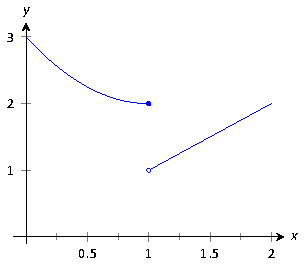
\includegraphics{test-figure2.pdf}
%  \captionof{figure}{Test caption}
%  \end{minipage}}}


%\newenvironment{mfigurefile}[2]{%
%\begin{tikzpicture}[remember picture,overlay]%
%\ifthenelse{\isodd{\thepage}}{\node [xshift=-36pt-.5\marginparwidth,yshift=#2\paperheight] at (current page.south east) }{\node [xshift=36pt+.5\marginparwidth,yshift=#2\paperheight] at (current page.south west) }%
%{\input{#1}};}%
%{\end{tikzpicture}%
%}

%\DeclareCaptionType{mytype}[Typename][List of mytype]


    
%%%%
%% End margin figure 
%%%%    
    

\newcommand{\bmx}[1]{\left[\hskip -3pt\begin{array}{#1} }
\newcommand{\emx}{\end{array}\hskip -3pt\right]}

\newcommand{\btz}{\begin{center}\begin{tikzpicture}}
\newcommand{\etz}{\end{tikzpicture}\end{center}}

\newcommand{\ds}{\displaystyle}

\newcommand{\fp}{\ensuremath{f\,'}}
\newcommand{\fpp}{\ensuremath{f\,''}}

\newcommand{\Fp}{\ensuremath{F\primeskip'}}
\newcommand{\Fpp}{\ensuremath{F\primeskip''}}

\newcommand{\yp}{\ensuremath{y\primeskip'}}
\newcommand{\gp}{\ensuremath{g\primeskip'}}

\newcommand{\dx}{\ensuremath{\Delta x}}
\newcommand{\dy}{\ensuremath{\Delta y}}
%\newcommand{\dz}{\ensuremath{\Delta z}}
\newcommand{\ddz}{\ensuremath{\Delta z}}

\newcommand{\thet}{\ensuremath{\theta}}
\newcommand{\norm}[1]{\ensuremath{||\ #1\ ||}}
\newcommand{\vnorm}[1]{\ensuremath{\norm{\vec #1}}}
\newcommand{\snorm}[1]{\ensuremath{\left|\left|\ #1\ \right|\right|}}
\newcommand{\la}{\left\langle}
\newcommand{\ra}{\right\rangle}
\newcommand{\dotp}[2]{\ensuremath{\vec #1 \cdot \vec #2}}
\newcommand{\proj}[2]{\ensuremath{\text{proj}_{\,\vec #2}{\,\vec #1}}}
\newcommand{\crossp}[2]{\ensuremath{\vec #1 \times \vec #2}}
\newcommand{\veci}{\ensuremath{\vec i}}
\newcommand{\vecj}{\ensuremath{\vec j}}
\newcommand{\veck}{\ensuremath{\vec k}}
\newcommand{\vecu}{\ensuremath{\vec u}}
\newcommand{\vecv}{\ensuremath{\vec v}}
\newcommand{\vecw}{\ensuremath{\vec w}}
\newcommand{\vecx}{\ensuremath{\vec x}}
\newcommand{\vecy}{\ensuremath{\vec y}}
\newcommand{\vrp}{\ensuremath{\vec r\, '}}
\newcommand{\vsp}{\ensuremath{\vec s\, '}}
\newcommand{\vrt}{\ensuremath{\vec r(t)}}
\newcommand{\vst}{\ensuremath{\vec s(t)}}
\newcommand{\vvt}{\ensuremath{\vec v(t)}}
\newcommand{\vat}{\ensuremath{\vec a(t)}}
\newcommand{\px}{\ensuremath{\partial x}}
\newcommand{\py}{\ensuremath{\partial y}}
\newcommand{\pz}{\ensuremath{\partial z}}
\newcommand{\pf}{\ensuremath{\partial f}}
\newcommand{\underlinespace}{\underline{\phantom{xxxxxx}}}

\newcommand{\mathN}{\ensuremath{\mathbb{N}}}

\newcommand{\zerooverzero}{\ensuremath{\ds \raisebox{8pt}{\text{``\ }}\frac{0}{0}\raisebox{8pt}{\text{\ ''}}}}


\newcommand{\myrule}{\rule[-4pt]{0pt}{13pt}}
\newcommand{\mmrule}{\rule[-10pt]{0pt}{15pt}}
\newcommand{\myds}{\ds\mmrule}
\newcommand{\deriv}[2]{\ensuremath{\myds\frac{d}{dx}\left(#1\right)=#2}}
\newcommand{\myint}[2]{\ensuremath{\myds\int #1\ dx=} \ensuremath{\ds #2}}

\DeclareMathOperator{\sech}{sech}
\DeclareMathOperator{\csch}{csch}

\newcommand{\sword}[1]{\textbf{#1}}

\newcommand{\primeskip}{\hskip.75pt}

%%%% Begin Header TikZ

%  Some TiKZ  shortcuts to help make drawing 3D vectors faster.
%

\newcommand{\plotlinecolor}{blue}

%
% Draw x and y tick marks
%
\newcommand{\drawxticks}[1]
{\foreach \x in {#1}
		{\draw  (\x,-.1)--(\x,.1);
			};
}
\newcommand{\drawyticks}[1]
{\foreach \x in {#1}
		{\draw  (-.1,\x)--(.1,\x);
			};
}

\newcommand{\drawxlines}[3]
{\draw[<->] (#1,0) -- (#2,0) node [right] {$x$};
\foreach \x in {#3}
		{\draw  (\x,-.1)--(\x,.1);
			};
}

\newcommand{\drawylines}[3]
{\draw[<->] (0,#1) -- (0,#2) node [above] {$y$};
\foreach \x in {#3}
		{\draw  (-.1,\x)--(.1,\x);
			};
}

\newcommand{\drawxlabels}[1]
{\foreach \x in {#1}
		{\draw  (\x,-.1) node [below] {\scriptsize $\x$};
		};
}

\newcommand{\drawylabels}[1]
{\foreach \x in {#1}
		{\draw  (-.1,\x) node [left] {\scriptsize $\x$};
		};
}

%% draw a box of margin width size to see if figure is properly contained within
\newcommand{\marginsizebox}{\draw (0,0)--(\marginparwidth,0)--(\marginparwidth,3)--(0,3)--cycle;}

%%%%
%%%%

\newcommand{\asyouread}[1]{\begin{tikzpicture}
\ifthenelse{\boolean{in_color}}{\node [preaction={fill=black,opacity=.5,transform canvas={xshift=1mm,yshift=-1mm}}, right color=blue!80!black!30, left color=blue!80] at (0,0) {\textcolor{white}{\textsf{\textit{AS YOU READ $\ldots$}}}};}
{\node [preaction={fill=black,opacity=.5,transform canvas={xshift=1mm,yshift=-1mm}}, right color=black!30, left color=black!10] at (0,0) {\textcolor{white}{\textsf{\textit{AS YOU READ $\ldots$}}}};}
\end{tikzpicture}
\begin{enumerate}
#1
\end{enumerate}
\vskip 20pt}

%%%%
%%  A new figure environment, trying to fix the float problem.
%%
%%%%

\newcounter{myfigurecounter}[chapter]
\renewcommand\themyfigurecounter{\thechapter.\arabic{myfigurecounter}}
\newenvironment{myfigure}{\refstepcounter{myfigurecounter}}{}
\newcommand{\mycaption}[1]{%
\begin{center}%
\vskip -1.5\baselineskip
\begin{tikzpicture}%
\draw (0,0) node [text width=\textwidth,align=center] {Figure \themyfigurecounter: #1};%
\end{tikzpicture}%
\end{center}%
}
\usepackage{pgfplots}
\pgfplotsset{compat=1.8}



\ifthenelse{\boolean{xetex}}%
	{\sffamily
	%%\usepackage{fontspec}
	\usepackage{mathspec}
	\setallmainfonts[Mapping=tex-text]{Calibri}
	\setmainfont[Mapping=tex-text]{Calibri}
	\setsansfont[Mapping=tex-text]{Calibri}
	\setmathsfont(Greek){[cmmi10]}}
	{\usepackage[sfdefault,lf]{carlito}
%% The 'lf' option for lining figures
%% The 'sfdefault' option to make the base font sans serif
\usepackage[T1]{fontenc}
\renewcommand*\oldstylenums[1]{\carlitoOsF #1}}
	
	\ifthenelse{\boolean{luatex}}%
	{\sffamily
	\usepackage{fontspec}
	\usepackage{unicode-math}
	%\usepackage{mathspec}
	%\setallmainfonts[Mapping=tex-text]{Calibri}
	\setmainfont{Calibri}
	%\setsansfont[Mapping=tex-text]{Calibri}
	\setmathfont[range=\mathup]{Calibri}
	\setmathfont[range=\mathit]{Calibri Italic}
	}
	{}

\makeindex

%%%\tracingonline=1
\begin{document}


%\printincolor
\printinblackandwhite

%\printexercisenames
%\printallanswers

%
%%%%%%%%%%
%%%
%%%  Set criteria for the format of the book.
%%%  This supercedes anything set in the Text_Header.
%%%
%%%%%%%%%%



%\printinblackandwhite

%\printexercisenames

%\nodrawexamplelines

%\printallanswers


\normalem



%%%\pagenumbering{roman}

%%%%%%
%%%		For editing purposes, block comment down to 
%%%		the next mark
%%%%%%

%%%%\input{cover/front_cover_in_text}
%%%%\clearpage
%%%%\thispagestyle{empty}
\frontmatter
%%%%
%%%%\title{\textsc{Fundamentals of Matrix Algebra}\\
%%%%{\small Version 2.1011}}
%%%%\author{Gregory N. Hartman, Ph.D.}
%%%%\date{}

\vspace*{\stretch{.5}}

\hskip 125pt\begin{minipage}{\textwidth}
\begin{flushright}

\textsc{{\Huge Math 2570 Calculus III}} \\

%\textsl{Third Edition}, 
{\large University of Lethbridge}\\

{A version of the \apex\ Calculus textbook edited by Sean Fitzpatrick}

\bigskip

\Large
%\vspace{1in}

Gregory Hartman, Ph.D.

\emph{\small Department of Applied Mathematics}

\emph{\small Virginia Military Institute}\vskip15pt

%Ji{\v r}\'i Lebl, Ph.D.

%\emph{\small Department of Mathematics}

%\emph{\small University of Oklahoma}

\parbox{200pt}{\textit{Contributing Authors}}\hskip 2cm \phantom{.}

Troy Siemers, Ph.D.

\emph{\small Department of Applied Mathematics}

\emph{\small Virginia Military Institute}\vskip 15pt

Brian Heinold, Ph.D.

\emph{\small Department of Mathematics and Computer Science}

\emph{\small Mount Saint Mary's University}\vskip 15pt

Dimplekumar Chalishajar, Ph.D.

\emph{\small Department of Applied Mathematics}

\emph{\small Virginia Military Institute}\vskip 25pt



\parbox{200pt}{\textit{Editor}}\hskip 2cm \phantom{.}
%\textit{Editor}\hskip 7cm\phantom{.}

Jennifer Bowen, Ph.D.

\emph{\small Department of Mathematics and Computer Science}

\emph{\small The College of Wooster}


\normalsize
\end{flushright}
\end{minipage}

\vspace{\stretch{1}}


\thispagestyle{empty}
\clearpage

\vspace*{\stretch{5}}
\noindent\hskip -1in\begin{minipage}{2in}
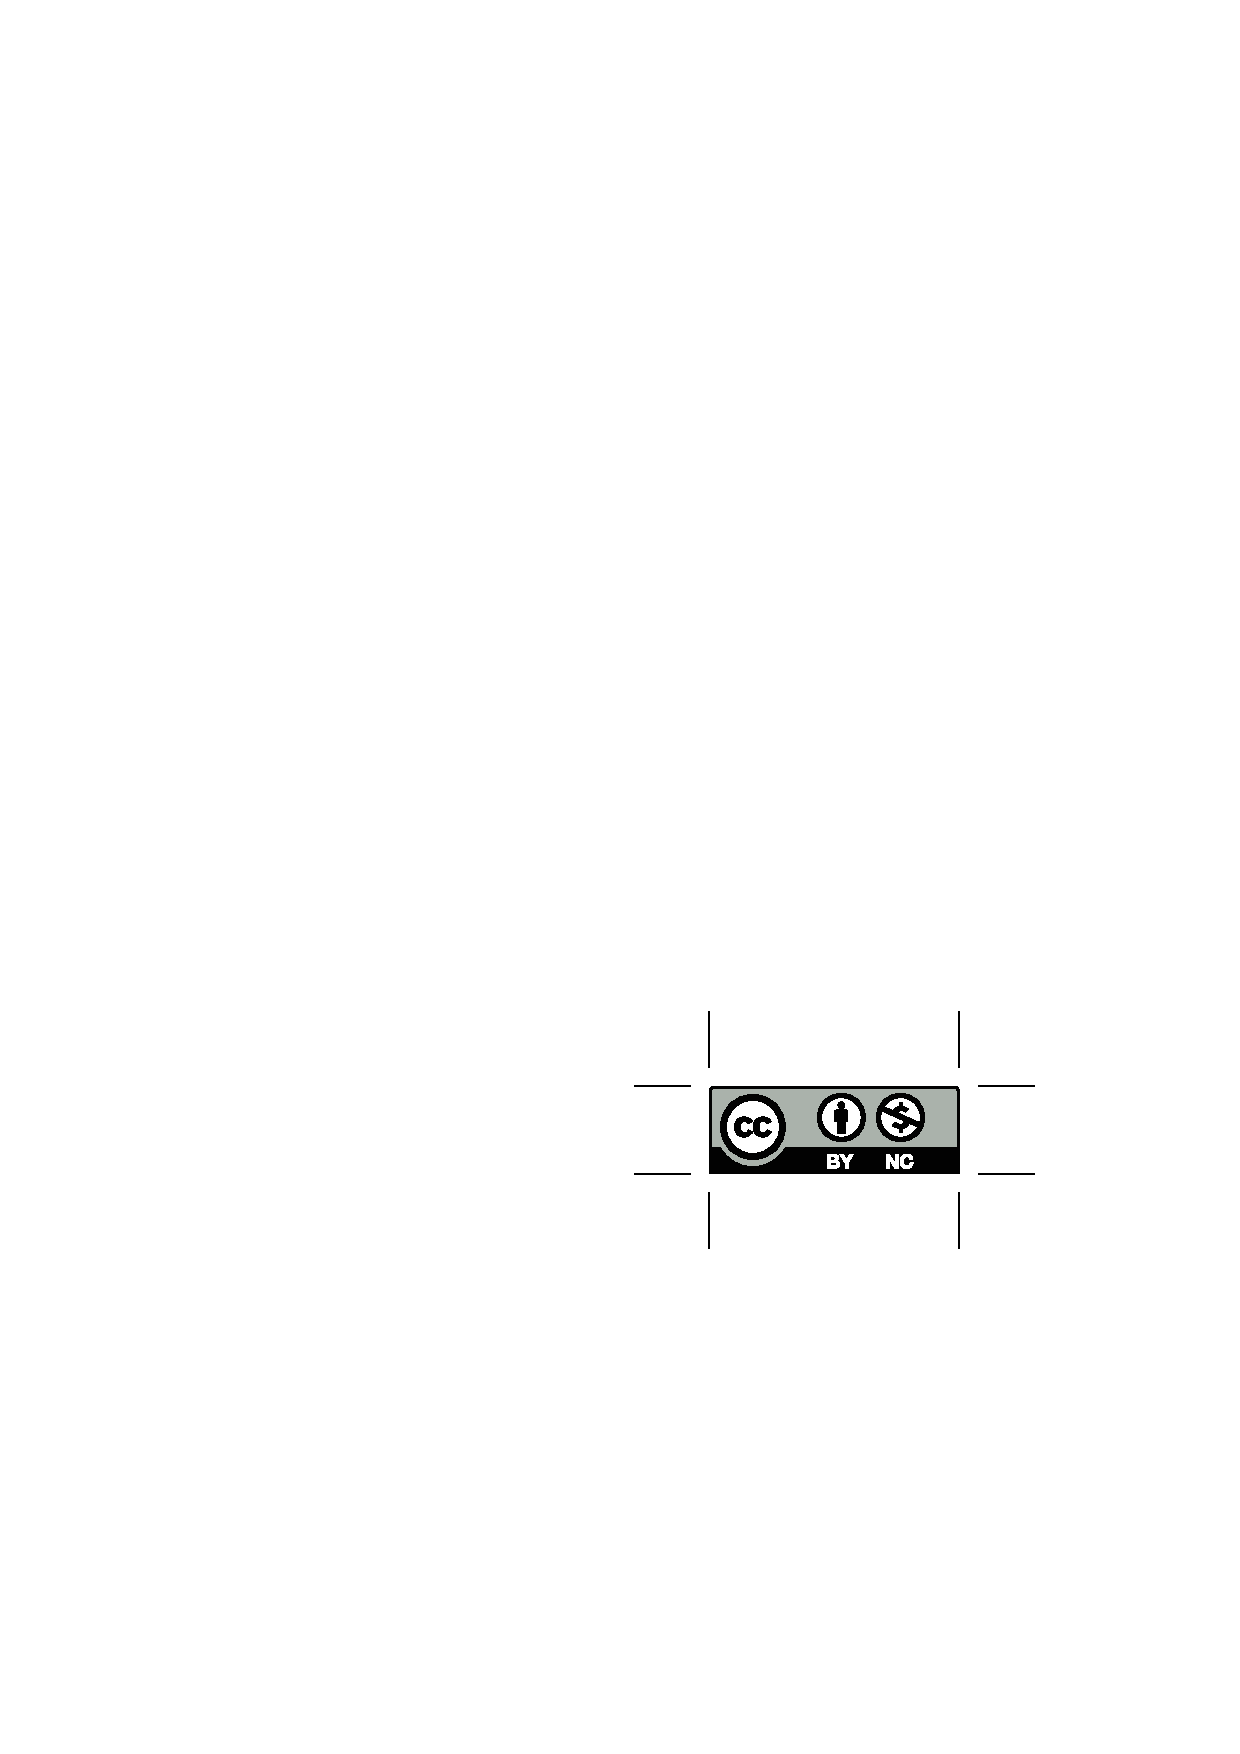
\includegraphics{text/by-nc} 
\end{minipage}
\begin{minipage}{3in}
\noindent Copyright \copyright\ 2018 Gregory Hartman

Licensed to the public under Creative Commons Attribution-Noncommercial 4.0 International Public License
\end{minipage}

\bigskip

\bigskip



\bigskip

\begin{minipage}{3.3in}
This version of the text was assembled and edited by Sean Fitzpatrick, University of Lethbridge, November 2015, revised most recently in May 2018. 

This work is licensed under the Creative Commons Attribution-Noncommercial-ShareAlike 4.0 International Public License
\end{minipage}
\vspace{\stretch{1}} 
\thispagestyle{empty}
\clearpage


%\cleardoublepage
%%%%\phantomsection
%%%%\input{text/thanks}
\addtocontents{toc}{\protect\thispagestyle{empty}}
%%%%\addcontentsline{toc}{chapter}{Thanks} 
%%%%\clearpage{\pagestyle{empty}\cleardoublepage}
%%%%\phantomsection
%%%%\thispagestyle{empty}
\Huge
\noindent {\bf \textsc{Preface}}\\
\large
\emph{A Note on Using this Text}
\vspace{1in}
\normalsize

Thank you for reading this short preface. Allow us to share a few key points about the text so that you may better understand what you will find beyond this page.

This text comprises a three--volume series on Calculus. The first part covers material taught in many ``Calc 1'' courses: limits, derivatives, and the basics of integration, found in Chapters 1 through 6.1. The second text covers material often taught in ``Calc 2:'' integration and its applications, along with an introduction to sequences, series and Taylor Polynomials, found in Chapters 5 through 8. The third text covers topics common in ``Calc 3'' or ``multivariable calc:'' parametric equations, polar coordinates, vector--valued functions, and functions of more than one variable, found in Chapters 9 through 13. All three are available separately for free at \texttt{\href{http://apexcalculus.com}{www.apexcalculus.com}}. %These three texts are intended to work together and make one cohesive text, \textit{APEX Calculus}, which can also be downloaded from the website. 

Printing the entire text as one volume makes for a large, heavy, cumbersome book. One can certainly only print the pages they currently need, but some prefer to have a nice, bound copy of the text. Therefore this text has been split into these three manageable parts, each of which can be purchased for under \$15 at \href{http://amazon.com}{Amazon.com}.\\ 



%A result of this splitting is that sometimes a concept is said to be explored in a ``later section,'' though that section does not actually appear in this particular text. Downloading the .pdf of \textit{APEX Calculus} will ensure that you have all the content.  
%material is referenced that is not contained in the present text. The context should make it clear whether the ``missing'' material is in the \textit{Calculus I} or \textit{Calculus III} portion. Downloading the appropriate .pdf, or the whole \textit{APEX Calculus} .pdf, will give access to these topics.
% This splitting of the material also results in unfortunate page/chapter numberings. Chapter 5 of this text is Chapter 1 of \textit{Calculus II}. Apart from these numberings, page--for--page the content of the sections that appear in both \textit{Calculus I} and \textit{Calculus II} are identical.\\ %For instance, in this text, ``Theorem 20'' may be mentioned, although Theorem 20 is only presented in Part I. To minimize confusion, theorems, definitions and key ideas are referenced by their title or subject matter, not their number.

%The current publisher of this text does not allow one text to be split across multiple volumes, with continuity of chapters and page numberings. This is the one drawback of the current publishing model that has many advantages, highlighted below. Because of this, there are a few peculiarities 

\noindent\textbf{\large For Students: How to Read this Text}\\

Mathematics textbooks have a reputation for being hard to read. High--level mathematical writing often seeks to say much with few words, and this style often seeps into texts of lower--level topics. This book was written with the goal of being easier to read than many other calculus textbooks, without becoming too verbose. 

Each chapter and section starts with an introduction of the coming material, hopefully setting the stage for ``why you should care,'' and ends with a look ahead to see how the just--learned material helps address future problems. 

\textit{Please read the text;} it is written to explain the concepts of Calculus. There are numerous examples to demonstrate the meaning of definitions, the truth of theorems, and the application of mathematical techniques. When you encounter a sentence you don't understand, read it again. If it still doesn't make sense, read on anyway, as sometimes confusing sentences are explained by later sentences.

\textit{You don't have to read every equation.} The examples generally show ``all'' the steps needed to solve a problem. Sometimes reading through each step is helpful; sometimes it is confusing. When the steps are illustrating a new technique, one probably should follow each step closely to learn the new technique. When the steps are showing the mathematics needed to find a number to be used later, one can usually skip ahead and see how that number is being used, instead of getting bogged down in reading how the number was found.

\textit{Most proofs have been omitted.} In mathematics, \textit{proving} something is always true is extremely important, and entails much more than testing to see if it works twice. However, students often are confused by the details of a proof, or become concerned that they should have been able to construct this proof on their own. To alleviate this potential problem, we do not include the proofs to most theorems in the text. The interested reader is highly encouraged to find proofs online or from their instructor. In most cases, one is very capable of understanding what a theorem \textit{means} and \textit{how to apply it} without knowing fully \textit{why} it is true.
\\

\thispagestyle{empty}
\noindent\textbf{\large Interactive, 3D Graphics}\\

New to Version 3.0 is the addition of interactive, 3D graphics in the .pdf version. Nearly all graphs of objects in space can be rotated, shifted, and zoomed in/out so the reader can better understand the object illustrated. 

As of this writing, the only pdf viewers that support these 3D graphics are Adobe Reader \& Acrobat (and only the versions for PC/Mac/Unix/Linux computers, not tablets or smartphones). To activate the interactive mode, click on the image. Once activated, one can click/drag to rotate the object and use the scroll wheel on a mouse to zoom in/out. (A great way to investigate an image is to first zoom in on the page of the pdf viewer so the graphic itself takes up much of the screen, then zoom inside the graphic itself.) A CTRL-click/drag pans the object left/right or up/down. By right-clicking on the graph one can access a menu of other options, such as changing the lighting scheme or perspective. One can also revert the graph back to its default view. If you wish to deactive the interactivity, one can right-click and choose the ``Disable Content'' option. \\

\noindent\textbf{\large Thanks}\\

There are many people who deserve recognition for the important role they have played in the development of this text. First, I thank Michelle for her support and encouragement, even as this ``project from work'' occupied my time and attention at home. Many thanks to Troy Siemers, whose most important contributions extend far beyond the sections he wrote or the 227 figures he coded in Asymptote for 3D interaction.  He provided incredible support, advice and encouragement for which I am very grateful. My thanks to Brian Heinold and Dimplekumar Chalishajar for their contributions and to Jennifer Bowen for reading through so much material and providing great feedback early on. Thanks to Troy, Lee Dewald, Dan Joseph, Meagan Herald, Bill Lowe, John David, Vonda Walsh, Geoff Cox, Jessica Libertini and other faculty of VMI who have given me numerous suggestions and corrections based on their experience with teaching from the text. (Special thanks to Troy, Lee \& Dan for their patience in teaching Calc III while I was still writing the Calc III material.) Thanks to Randy Cone for encouraging his tutors of VMI's Open Math Lab to read through the text and check the solutions, and thanks to the tutors for spending their time doing so. A very special thanks to Kristi Brown and Paul Janiczek who took this opportunity far above \& beyond what I expected, meticulously checking every solution and carefully reading every example. Their comments have been extraordinarily helpful. I am also thankful for the support provided by Wane Schneiter, who as my Dean provided me with extra time to work on this project. I am blessed to have so many people give of their time to make this book better.\\

\noindent\textbf{\large \apex\  -- Affordable Print and Electronic teXts}\\

\apex\ is a consortium of authors  who collaborate to produce high--quality, low--cost textbooks. The current textbook--writing paradigm is facing a potential revolution as desktop publishing and electronic formats increase in popularity. However, writing a good textbook is no easy task, as the time requirements alone are substantial. It takes countless hours of work to produce text, write examples and exercises, edit and publish. Through collaboration, however, the cost to any individual can be lessened, allowing us to create texts that we freely distribute electronically and sell in printed form for an incredibly low cost. Having said that, nothing is entirely free; someone always bears some cost. This text ``cost'' the authors of this book their time, and that was not enough. \textit{APEX Calculus} would not exist had not the Virginia Military Institute, through a generous Jackson--Hope grant, given the lead author significant time away from teaching so he could focus on this text.

Each text is available as a free .pdf, protected by a Creative Commons Attribution - Noncommercial 4.0 copyright. That  means you can give the .pdf to anyone you like, print it in any form you like, and even edit the original content and redistribute it. If you do the latter, you must  clearly reference this work and you cannot sell your edited work for money.

We encourage others to adapt this work to fit their own needs. One might add sections that are ``missing'' or remove sections that your students won't need. The source files can be found at \texttt{\href{https://github.com/APEXCalculus}{github.com/APEXCalculus}}.

You can learn more at \texttt{\href{http://www.vmi.edu/APEX}{www.vmi.edu/APEX}}.
\thispagestyle{empty}


%%%%\addcontentsline{toc}{chapter}{Preface}
%%%%\clearpage{\pagestyle{empty}\cleardoublepage}
%%%%\phantomsection
%%%%

\addcontentsline{toc}{chapter}{Table of Contents}
\tableofcontents
\clearpage{\pagestyle{empty}\cleardoublepage}

\phantomsection
\prefacegeometry
\addcontentsline{toc}{chapter}{Preface}
\thispagestyle{empty}
\Huge
\noindent {\bf \textsc{Preface}}\\

This is an open textbook based on the \apex\ textbook series by Gregory Hartman et al. The book is made available free of charge, and has been customized to meet the curriculum for Math 2570 at the University of Lethbridge.

The topics for Math 2570, as laid out in the Academic Calendar, correspond to Chapters 10-13 of this textbook, with the following notes:
\begin{itemize}
\item I have also included Chapter 9, on parametric and polar curves. This material is officially part of Math 2560 (Calculus II), but it is often given superficial treatment (or skipped altogether) due to time constraints.

Your Math 2570 instructor will probably choose to cover/review this material, since it is good preparation for the material in Chapter 12, on vector-valued functions.

\item Typically Math 2570 only covers the first few sections of Chapter 13, on functions of several variables. Most instructors get as far as partial derivatives, but no further. I've included the whole chapter in case there is time to go further, and for those students who are interested. The content of Chapter 13 is usually where Calculus IV (Math 2580) begins.
\end{itemize}

Aside from reorganization, the content of this text is essentially unaltered from its form in the original \apex\ textbooks. The book has not yet been adopted for use in Math 2570, so there has not been any incentive to invest the time required to carefully edit the text.

I have included the preface from the original authors below. If you choose to use this text, please let me know if you find any areas for improvement.

\vspace{1in}

\begin{flushright}
Sean Fitzpatrick\\
Department of Mathematics and Computer Science\\
University of Lethbridge\\
August, 2017
\end{flushright}

\newpage
\large
\emph{A Note on Using this Text}
\vskip 2\baselineskip
\normalsize

Thank you for reading this short preface. Allow us to share a few key points about the text so that you may better understand what you will find beyond this page.

This text is Part III of a three--text series on Calculus. The first part covers material taught in many ``Calc 1'' courses: limits, derivatives, and the basics of integration, found in Chapters 1 through 6.1. The second text covers material often taught in ``Calc 2:'' integration and its applications, along with an introduction to sequences, series and Taylor Polynomials, found in Chapters 5 through 8. The third text covers topics common in ``Calc 3'' or ``multivariable calc:'' parametric equations, polar coordinates, vector--valued functions, and functions of more than one variable, found in Chapters 9 through 13. All three are available separately for free at \texttt{\href{http://www.vmi.edu/APEX}{www.vmi.edu/APEX}}. These three texts are intended to work together and make one cohesive text, \textit{APEX Calculus}, which can also be downloaded from the website. 

Printing the entire text as one volume makes for a large, heavy, cumbersome book. One can certainly only print the pages they currently need, but some prefer to have a nice, bound copy of the text. Therefore this text has been split into these three manageable parts, each of which can be purchased for under \$15 at \href{http://amazon.com}{Amazon.com}. 

A result of this splitting is that sometimes a concept is said to be explored in an ``earlier section,'' though that section does not actually appear in this particular text. Also, the index makes reference to topics, and page numbers, that do not appear in this text. This is done intentionally to show the reader what topics are available for study.  Downloading the .pdf of \textit{APEX Calculus} will ensure that you have all the content.\\ 
%material is referenced that is not contained in the present text. The context should make it clear whether the ``missing'' material is in the \textit{Calculus I} or \textit{Calculus III} portion. Downloading the appropriate .pdf, or the whole \textit{APEX Calculus} .pdf, will give access to these topics.
  %For instance, in this text, ``Theorem 20'' may be mentioned, although Theorem 20 is only presented in Part I. To minimize confusion, theorems, definitions and key ideas are referenced by their title or subject matter, not their number.

%The current publisher of this text does not allow one text to be split across multiple volumes, with continuity of chapters and page numberings. This is the one drawback of the current publishing model that has many advantages, highlighted below. Because of this, there are a few peculiarities 

\noindent\textbf{\large For Students: How to Read this Text}\\

Mathematics textbooks have a reputation for being hard to read. High--level mathematical writing often seeks to say much with few words, and this style often seeps into texts of lower--level topics. This book was written with the goal of being easier to read than many other calculus textbooks, without becoming too verbose. 

Each chapter and section starts with an introduction of the coming material, hopefully setting the stage for ``why you should care,'' and ends with a look ahead to see how the just--learned material helps address future problems. 

\textit{Please read the text;} it is written to explain the concepts of Calculus. There are numerous examples to demonstrate the meaning of definitions, the truth of theorems, and the application of mathematical techniques. When you encounter a sentence you don't understand, read it again. If it still doesn't make sense, read on anyway, as sometimes confusing sentences are explained by later sentences.

\textit{You don't have to read every equation.} The examples generally show ``all'' the steps needed to solve a problem. Sometimes reading through each step is helpful; sometimes it is confusing. When the steps are illustrating a new technique, one probably should follow each step closely to learn the new technique. When the steps are showing the mathematics needed to find a number to be used later, one can usually skip ahead and see how that number is being used, instead of getting bogged down in reading how the number was found.

\textit{Most proofs have been omitted.} In mathematics, \textit{proving} something is always true is extremely important, and entails much more than testing to see if it works twice. However, students often are confused by the details of a proof, or become concerned that they should have been able to construct this proof on their own. To alleviate this potential problem, we do not include the proofs to most theorems in the text. The interested reader is highly encouraged to find proofs online or from their instructor. In most cases, one is very capable of understanding what a theorem \textit{means} and \textit{how to apply it} without knowing fully \textit{why} it is true.
\\

\thispagestyle{empty}
\noindent\textbf{\large Interactive, 3D Graphics}\\

New to Version 3.0 is the addition of interactive, 3D graphics in the .pdf version. Nearly all graphs of objects in space can be rotated, shifted, and zoomed in/out so the reader can better understand the object illustrated. 

As of this writing, the only pdf viewers that support these 3D graphics are Adobe Reader \& Acrobat (and only the versions for PC/Mac/Unix/Linux computers, not tablets or smartphones). To activate the interactive mode, click on the image. Once activated, one can click/drag to rotate the object and use the scroll wheel on a mouse to zoom in/out. (A great way to investigate an image is to first zoom in on the page of the pdf viewer so the graphic itself takes up much of the screen, then zoom inside the graphic itself.) A CTRL-click/drag pans the object left/right or up/down. By right-clicking on the graph one can access a menu of other options, such as changing the lighting scheme or perspective. One can also revert the graph back to its default view. If you wish to deactive the interactivity, one can right-click and choose the ``Disable Content'' option. \\

\noindent\textbf{\large Thanks}\\

There are many people who deserve recognition for the important role they have played in the development of this text. First, I thank Michelle for her support and encouragement, even as this ``project from work'' occupied my time and attention at home. Many thanks to Troy Siemers, whose most important contributions extend far beyond the sections he wrote or the 227 figures he coded in Asymptote for 3D interaction.  He provided incredible support, advice and encouragement for which I am very grateful. My thanks to Brian Heinold and Dimplekumar Chalishajar for their contributions and to Jennifer Bowen for reading through so much material and providing great feedback early on. Thanks to Troy, Lee Dewald, Dan Joseph, Meagan Herald, Bill Lowe, John David, Vonda Walsh, Geoff Cox, Jessica Libertini and other faculty of VMI who have given me numerous suggestions and corrections based on their experience with teaching from the text. (Special thanks to Troy, Lee \& Dan for their patience in teaching Calc III while I was still writing the Calc III material.) Thanks to Randy Cone for encouraging his tutors of VMI's Open Math Lab to read through the text and check the solutions, and thanks to the tutors for spending their time doing so. A very special thanks to Kristi Brown and Paul Janiczek who took this opportunity far above \& beyond what I expected, meticulously checking every solution and carefully reading every example. Their comments have been extraordinarily helpful. I am also thankful for the support provided by Wane Schneiter, who as my Dean provided me with extra time to work on this project. I am blessed to have so many people give of their time to make this book better.\\

\clearpage
\noindent\textbf{\large \apex\  -- Affordable Print and Electronic teXts}\\

\apex\ is a consortium of authors  who collaborate to produce high--quality, low--cost textbooks. The current textbook--writing paradigm is facing a potential revolution as desktop publishing and electronic formats increase in popularity. However, writing a good textbook is no easy task, as the time requirements alone are substantial. It takes countless hours of work to produce text, write examples and exercises, edit and publish. Through collaboration, however, the cost to any individual can be lessened, allowing us to create texts that we freely distribute electronically and sell in printed form for an incredibly low cost. Having said that, nothing is entirely free; someone always bears some cost. This text ``cost'' the authors of this book their time, and that was not enough. \textit{APEX Calculus} would not exist had not the Virginia Military Institute, through a generous Jackson--Hope grant, given the lead author significant time away from teaching so he could focus on this text.

Each text is available as a free .pdf, protected by a Creative Commons Attribution - Noncommercial 4.0 copyright. That  means you can give the .pdf to anyone you like, print it in any form you like, and even edit the original content and redistribute it. If you do the latter, you must  clearly reference this work and you cannot sell your edited work for money.

We encourage others to adapt this work to fit their own needs. One might add sections that are ``missing'' or remove sections that your students won't need. The source files can be found at \texttt{\href{https://github.com/APEXCalculus}{github.com/APEXCalculus}}.

You can learn more at \texttt{\href{http://www.vmi.edu/APEX}{www.vmi.edu/APEX}}.
\thispagestyle{empty}


\restoregeometry
\clearpage{\pagestyle{empty}\cleardoublepage}

%%%%
\mainmatter


%%%%
%		End block comment here
%%%%







%\setcounterref{definitioncounter}{29}
\addtocounter{definitioncounter}{28}
%\setcounterref{theoremcounter}{62}
\addtocounter{theoremcounter}{61}
%\setcounterref{keyideacounter}{31}
\addtocounter{keyideacounter}{30}
%\setcounterref{examplecounter}{264}
\addtocounter{examplecounter}{263}


\addtocounter{page}{386}
\addtocounter{chapter}{8}

\clearpage{\pagestyle{empty}\cleardoublepage}
\chapter{Curves in the Plane}
\thispagestyle{empty}
We have explored functions of the form $y=f(x)$ closely throughout this text. We have explored their limits, their derivatives and their antiderivatives; we have learned to identify key features of their graphs, such as relative maxima and minima, inflection points and asymptotes; we have found equations of their tangent lines, the areas between portions of their graphs and the $x$-axis, and the volumes of solids generated by revolving portions of their graphs about a horizontal or vertical axis.

Despite all this, the graphs created by functions of the form $y=f(x)$ are limited. Since each $x$-value can correspond to only 1 $y$-value, common shapes like circles cannot be fully described by a function in this form.  Fittingly, the ``vertical line test''  excludes vertical lines from being functions of $x$, even though these lines are important in mathematics.

In this chapter we'll explore new ways of drawing curves in the plane. We'll still work within the framework of functions, as an input will still only correspond to one output. However, our new techniques of drawing curves will render the vertical line test pointless, and allow us to create important -- and beautiful -- new curves. Once these curves are defined, we'll apply the concepts of calculus to them, continuing to find equations of tangent lines and the areas of enclosed regions. 

\enlargethispage{15\baselineskip}

\section{Conic Sections}\label{sec:conic_sections}

The ancient Greeks recognized that interesting shapes can be formed by intersecting a plane with a 
\textit{double napped} cone (i.e., two identical cones placed tip--to--tip as shown in the following figures). As these shapes are formed as sections of conics, they have earned the official name ``conic sections.''

The three ``most interesting\primeskip'' conic sections are given in the top row of Figure \ref{fig:nondeg_conic}. They are the parabola, the ellipse (which includes circles) and the hyperbola. In each of these cases, the plane does not intersect the tips of the cones (usually taken to be the origin). \\

\noindent\begin{minipage}{\textwidth+50pt}
\noindent\centering
\begin{tabular}{cccc}
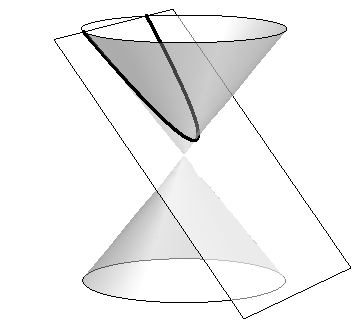
\includegraphics[scale=.25]{figures/conic_parabola}&
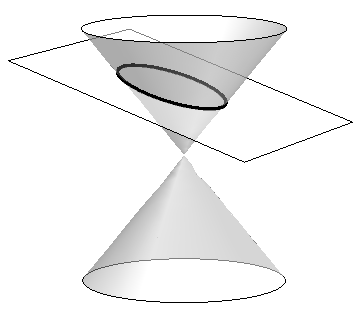
\includegraphics[scale=.25]{figures/conic_ellipse}&
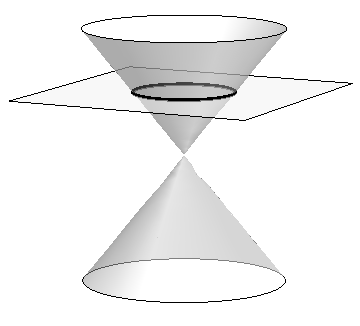
\includegraphics[scale=.25]{figures/conic_circle}&
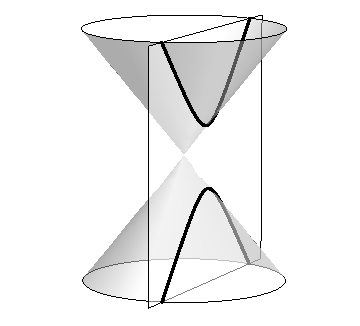
\includegraphics[scale=.25]{figures/conic_hyperbola} \\
\small Parabola &\small Ellipse & \small Circle &  \small Hyperbola
\end{tabular}
\vskip \baselineskip
\noindent%
\begin{tabular}{ccc}
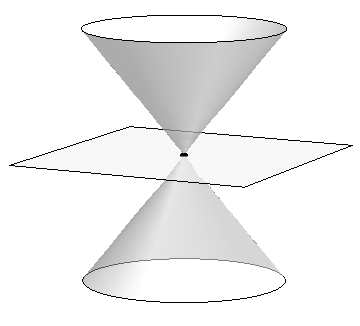
\includegraphics[scale=.25]{figures/conic_singlept}&
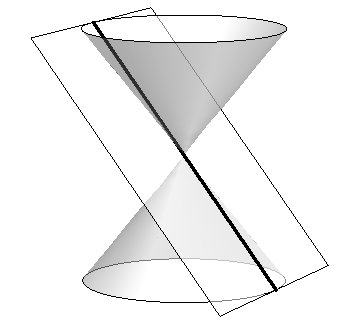
\includegraphics[scale=.25]{figures/conic_oneline}&
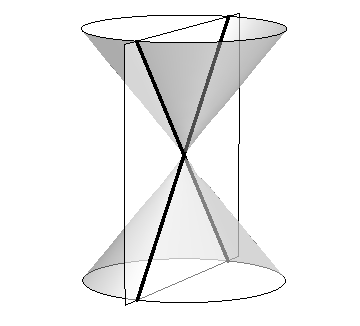
\includegraphics[scale=.25]{figures/conic_crossedlines}
\\
 \small Point& \small Line &\small  Crossed Lines 
\end{tabular}
\captionsetup{type=figure}%
\caption{Conic Sections}\label{fig:nondeg_conic}
\end{minipage}
\vskip\baselineskip

\clearpage

When the plane does contain the origin, three \textbf{degenerate} cones can be formed as shown the bottom row of  Figure \ref{fig:nondeg_conic}: a point, a line, and crossed lines. We focus here on the nondegenerate cases. \index{conic sections}\index{conic sections!degenerate}

While the above geometric constructs define the conics in an intuitive, visual way, these constructs are not very helpful when trying to analyze the shapes algebraically or consider them as the graph of a function. It can be shown that all conics can be defined by the general second--degree equation 
\[
Ax^2+Bxy+Cy^2+Dx+Ey+F=0.
\]
While this algebraic definition has its uses, most find another geometric perspective of the conics more beneficial.

Each nondegenerate conic can be defined as the \textbf{locus}, or set, of points that satisfy a certain distance property. These distance properties can be used to generate an algebraic formula, allowing us to study each conic as the graph of a function.\\

\noindent\textbf{\Large Parabolas}\\
%
%We start with a definition.
%
\definition{def:parabola}{Parabola}
{A \textbf{parabola} is the locus of all points equidistant from a point (called a \textbf{focus}) and a line (called the \textbf{directrix}) that does not contain the focus.
\index{conic sections!parabola}\index{parabola!definition}\index{directrix}\index{focus}
}

\mfigure{.4}{Illustrating the definition of the parabola and establishing an algebraic formula.}{fig:parabola_def}{figures/figparabola_def}
Figure \ref{fig:parabola_def} illustrates this definition. The point halfway between the focus and the directrix is the \textbf{vertex}. The line through the focus, perpendicular to the directrix, is the \textbf{axis of symmetry}, as the portion of the parabola on one side of this line is the mirror--image of the portion on the opposite side.

The definition leads us to an algebraic formula for the parabola. Let $P=(x,y)$ be a point on a parabola whose focus is at $F=(0,p)$ and whose directrix is at $y=-p$. (We'll assume for now that the focus lies on the $y$-axis; by placing the focus $p$ units above the $x$-axis and the directrix $p$ units below this axis, the vertex will be at $(0,0)$.)

We use the Distance Formula to find the distance $d_1$ between $F$ and $P$:
\[
d_1=\sqrt{(x-0)^2+(y-p)^2}.
\]
The distance $d_2$ from $P$ to the directrix is more straightforward:
\[
d_2=y-(-p) = y+p.
\]
These two distances are equal. Setting $d_1=d_2$, we can solve for $y$ in terms of $x$:
	\begin{align*}
	d_1&= d_2 \\
	\sqrt{x^2+(y-p)^2} &= y+p 
	\intertext{Now square both sides.}
	x^2+(y-p)^2 &= (y+p)^2 \\
	x^2+y^2-2yp+p^2 &= y^2+2yp+p^2\\
	x^2 &=4yp\\
	y&= \frac{1}{4p}x^2.
	\end{align*}
	The geometric definition of the parabola has led us to the familiar quadratic function whose graph is a parabola with vertex at the origin. When we allow the vertex to not be at $(0,0)$, we get the following standard form of the parabola.
	
	\keyidea{idea:parabola}{General Equation of a Parabola}
	{\begin{enumerate}
	\item		\textbf{Vertical Axis of Symmetry:} The equation of the parabola with vertex at $(h,k)$ and directrix $y=k-p$ in standard form is 
	\[
	y=\frac{1}{4p}(x-h)^2+k.
	\] 
	The focus is at $(h,k+p)$.
	\item		\textbf{Horizontal Axis of Symmetry:} The  equation of the parabola with vertex at $(h,k)$ and directrix $x=h-p$ in standard form is 
	\[
	x=\frac{1}{4p}(y-k)^2+h.
	\]
	The focus is at $(h+p,k)$.
	\end{enumerate}
	Note: $p$ is not necessarily a positive number.
	\index{parabola!general equation}
	}
	\enlargethispage{2\baselineskip}
	
	\example{ex_conic1}{Finding the equation of a parabola}{
	Give the equation of the parabola with focus at $(1,2)$ and directrix at $y=3$.}
	{The vertex is located halfway between the focus and directrix, so $(h,k) = (1,2.5)$. This gives $p=-0.5$. Using Key Idea \ref{idea:parabola} we have the equation of the parabola as 
	\[
	y=\frac{1}{4(-0.5)}(x-1)^2+2.5 = -\frac12(x-1)^2+2.5.
	\]
	\mfigure{.45}{The parabola described in Example \ref{ex_conic1}.}{fig:conic1}{figures/figconic1}
	The parabola is sketched in Figure \ref{fig:conic1}.
	}\\
	
	\example{ex_conic2}{Finding the focus and directrix of a parabola}{
	Find the focus and directrix of the parabola $x=\frac18y^2-y+1$. The point $(7,12)$ lies on the graph of this parabola; verify that it is equidistant from the focus and directrix.}
	{We need to put the equation of the parabola in its general form. This requires us to complete the square:
	\begin{align*}
	x &= \frac18y^2-y+1 \\
	&= \frac18\big(y^2-8y+8\big)\\
	&=	\frac18\big(y^2-8y+16 -16+8\big)\\
	&=	\frac18\big((y-4)^2 - 8\big)\\
	&=	\frac18(y-4)^2 -1.
	\end{align*}
	Hence the vertex is located at $(-1,4)$.  We have $\frac18=\frac1{4p}$, so $p=2$. We conclude that the focus is located at $(1,4)$ and the directrix is  $x=-3$. The parabola is graphed in Figure \ref{fig:conic2}, along with its focus and directrix.\\
	
\mfigure{.2}{The parabola described in Example \ref{ex_conic2}. The distances from a point on the parabola to the focus and directrix is given.}{fig:conic2}{figures/figconic2}
	
	The point $(7,12)$ lies on the graph and is $7-(-3)=10$ units from the directrix. The distance from $(7,12)$ to the focus is:
	\[
	\sqrt{(7-1)^2 + (12-4)^2} = \sqrt{100}=10.
	\]
	Indeed, the point on the parabola is equidistant from the focus and directrix.
	}\\
	
	\vskip\baselineskip
	\noindent\textbf{\large Reflective Property}
	\vskip\baselineskip
	
	One of the fascinating things about the nondegenerate conic sections is their reflective properties. Parabolas have the following reflective property:
	
	\hskip 20pt \begin{minipage}[t]{.8\linewidth}
	Any ray emanating from the focus that intersects the parabola reflects off along a line perpendicular to the directrix.
	\end{minipage}\\
	\enlargethispage{\baselineskip}
	
	This is illustrated in Figure \ref{fig:conic_reflect}. The following theorem states this more rigorously.
\mfigure{.3}{Illustrating the parabola's reflective property.}{fig:conic_reflect}{figures/figconic_reflect}
	
	\theorem{thm:parabola_reflect}{Reflective Property of the Parabola}
	{Let $P$ be a point on a parabola. The tangent line to the parabola at $P$ makes equal angles with the following two lines:
		\begin{enumerate}
		\item		The line containing $P$ and the focus $F$, and
		\item		The line perpendicular to the directrix through $P$.
		\index{parabola!reflective property}
		\end{enumerate}
	}
	
	Because of this reflective property, paraboloids (the 3D analogue of parabolas) make for useful flashlight reflectors as the light from the bulb, ideally located at the focus, is reflected along parallel rays. Satellite dishes also have paraboloid shapes. Signals coming from satellites effectively approach the dish along parallel rays. The dish then \textit{focuses} these rays at the focus, where the sensor is located.\\
\pagebreak
	
	\noindent\textbf{\Large Ellipses}
	\vskip \baselineskip
	
	\definition{def:ellipse}{Ellipse}
	{An \textbf{ellipse} is the locus of all points whose sum of distances from two fixed points, each a \textbf{focus} of the ellipse, is constant.\index{conic sections!ellipse}\index{ellipse!definition}\index{focus}
	}
	
	An easy way to visualize this construction of an ellipse is to pin both ends of a string to a board. The pins become the foci. Holding a pencil tight against the string places the pencil on the ellipse; the sum of distances from the pencil to the pins is constant: the length of the string. See Figure \ref{fig:ellipse_def}.
	\mfigure{.7}{Illustrating the construction of an ellipse with pins, pencil and string.}{fig:ellipse_def}{figures/figellipse_def}
	
	We can again find an algebraic equation for an ellipse using this geometric definition. Let the foci be located along the $x$-axis, $c$ units from the origin. Let these foci be labelled as $F_1 = (-c,0)$ and $F_2=(c,0)$. Let $P=(x,y)$ be a point on the ellipse. The sum of distances from $F_1$ to $P$ ($d_1$) and from $F_2$ to $P$ ($d_2$) is a constant $d$. That is, $d_1+d_2=d$. Using the Distance Formula, we have 
	\[
	\sqrt{(x+c)^2+y^2} + \sqrt{(x-c)^2+y^2} = d.
	\]
	Using a fair amount of algebra can produce the following equation of an ellipse (note that the equation is an implicitly defined function; it has to be, as an ellipse fails the Vertical Line Test):
	\[
	\frac{x^2}{\left(\frac d2\right)^2} + \frac{y^2}{\left(\frac d2\right)^2-c^2} = 1.
	\]
	This is not particularly illuminating, but by making the substitution $a=d/2$ and $b=\sqrt{a^2-c^2}$, we can rewrite the above equation as 
	\[
	\frac{x^2}{a^2} + \frac{y^2}{b^2} = 1.
	\]
	This choice of $a$ and $b$ is not without reason; as shown in Figure \ref{fig:ellipse_label}, the values of $a$ and $b$ have geometric meaning in the graph of the ellipse. 
\mfigure{.25}{Labelling the significant features of an ellipse.}{fig:ellipse_label}{figures/figellipse_label}
	
	In general, the two foci of an ellipse lie on the \textbf{major axis} of the ellipse, and the midpoint of the segment joining the two foci is the \textbf{center}. The major axis intersects the ellipse at two points, each of which is a \textbf{vertex}. The line segment through the center and perpendicular to the major axis is the \textbf{minor axis}. The ``constant sum of distances'' that defines the ellipse is the length of the major axis, i.e., $2a$.
	
	Allowing for the shifting of the ellipse gives the following standard equations.
	
	\keyidea{idea:ellipse}{Standard Equation of the Ellipse}
	{The equation of an ellipse centered at $(h,k)$ with major axis of length $2a$ and minor axis of length $2b$ in standard form is:
	\begin{enumerate}
	\item	\textbf{Horizontal major axis:} $\ds \frac{(x-h)^2}{a^2}+\frac{(y-k)^2}{b^2}=1.$
	
	\item	\textbf{Vertical major axis:} $\ds \frac{(x-h)^2}{b^2}+\frac{(y-k)^2}{a^2}=1.$
	\end{enumerate}
	The foci lie along the major axis, $c$ units from the center, where $c^2=a^2-b^2$.
	\index{ellipse!standard equation}
	}
	
	\example{ex_conic3}{Finding the equation of an ellipse}{
	Find the general equation of the ellipse graphed in Figure \ref{fig:conic3}.}
	{The center is located at $(-3,1)$. The distance from the center to a vertex is 5 units, hence $a=5$. The minor axis seems to have length 4, so $b=2$. Thus the equation of the ellipse is 
	\[
	\frac{(x+3)^2}{4}+\frac{(y-1)^2}{25} = 1.
	\]
	\mfigure{.65}{The ellipse used in Example \ref{ex_conic3}.}{fig:conic3}{figures/figconic3}
	}\\
	
\example{ex_conic4}{Graphing an ellipse}{
Graph the ellipse defined by $4x^2+9y^2-8x-36y=-4$.}
{It is simple to graph an ellipse once it is in standard form. In order to put the given equation in standard form, we must complete the square with both the $x$ and $y$ terms. We first rewrite the equation by regrouping:
\[
4x^2+9y^2-8x-36y=-4 \quad \Rightarrow \quad (4x^2-8x) + (9y^2-36y) = -4.
\]
Now we complete the squares.
\begin{align*}
(4x^2-8x) + (9y^2-36y) &= -4\\
4(x^2-2x) + 9(y^2-4y) &= -4 \\
4(x^2-2x +1 - 1) + 9(y^2-4y+4-4) &= - 4\\
4\big((x-1)^2-1\big) + 9\big((y-2)^2-4\big) &= -4\\
4(x-1)^2 -4 + 9(y-2)^2-36 &= -4 \\
4(x-1)^2 + 9(y-2)^2 &= 36 \\
\frac{(x-1)^2}{9} + \frac{(y-2)^2}{4} &= 1.
\end{align*}
We see the center of the ellipse is at $(1,2)$. We have $a=3$ and $b=2$; the major axis is horizontal, so the vertices are located at $(-2,2)$ and $(4,2)$. We find $c=\sqrt{9-4} = \sqrt{5}\approx 2.24.$ The foci are located along the major axis, approximately $2.24$ units from the center, at $(1\pm 2.24,2)$. This is all graphed in Figure \ref{fig:conic4}
\mfigure{.3}{Graphing the ellipse in Example \ref{ex_conic4}.}{fig:conic4}{figures/figconic4}.
}\\
\pagebreak

\noindent\textbf{\large Eccentricity}
\vskip\baselineskip

When $a=b$, we have a circle. The general equation becomes 
\[
\frac{(x-h)^2}{a^2} + \frac{(y-k)^2}{a^2} = 1 \quad \Rightarrow (x-h)^2 + (y-k)^2 = a^2,
\]
the familiar equation of the circle centred at $(h,k)$ with radius $a$.  Since $a=b$, $c = \sqrt{a^2-b^2}=0$. The circle has ``two'' foci, but they lie on the same point, the center of the circle. 



Consider Figure \ref{fig:ellipse_ecc}, where several ellipses are graphed with $a=1$. In (a), we have $c=0$ and the ellipse is a circle. As $c$ grows, the resulting ellipses look less and less circular. A measure of this ``noncircularness'' is \textit{eccentricity}.

\mtable{.6}{Understanding the eccentricity of an ellipse.}{fig:ellipse_ecc}{%
\begin{tabular}{c}
\myincludegraphics[scale=.75]{figures/figellipse_ecca}\\
(a)\\
\myincludegraphics[scale=.75]{figures/figellipse_eccb}\\
(b)\\
\myincludegraphics[scale=.75]{figures/figellipse_eccc}\\
(c)\\
\myincludegraphics[scale=.75]{figures/figellipse_eccd}\\
(d)
\end{tabular}
}

\definition{def:eccentricity_ellipse}{Eccentricity of an Ellipse}
{The eccentricity $e$ of an ellipse  is $\ds e=\frac{c}{a}$.
\index{ellipse!eccentricity}\index{eccentricity}
}

The eccentricity of a circle is 0; that is, a circle has no ``noncircularness.'' As $c$ approaches $a$, $e$ approaches 1, giving rise to a very noncircular ellipse, as seen in Figure \ref{fig:ellipse_ecc} (d). 

It was long assumed that planets had circular orbits. This is known to be incorrect; the orbits are elliptical. Earth has an eccentricity of $0.0167$ -- it has a nearly circular orbit.   Mercury's orbit is the most eccentric, with $e=0.2056$. (Pluto's eccentricity is greater, at $e=0.248$, the greatest of all the currently known dwarf planets.) The planet with the most circular orbit is Venus, with $e=0.0068$. The Earth's moon has an eccentricity of $e=0.0549$, also very circular.\\



\noindent \textbf{\large Reflective Property}
\vskip\baselineskip

The ellipse also possesses an interesting reflective property. Any ray emanating from one focus of an ellipse reflects off the ellipse along a line through the other focus, as illustrated in Figure \ref{fig:ellipse_reflect}. This property is given formally in the following theorem.

\mfigure{.2}{Illustrating the reflective property of an ellipse.}{fig:ellipse_reflect}{figures/figellipse_reflect}

\theorem{thm:ellipse_reflect}{Reflective Property of an Ellipse}
{Let $P$ be a point on a ellipse with foci $F_1$ and $F_2$. The tangent line to the ellipse at $P$ makes equal angles with the following two lines:\index{ellipse!reflective property}
\begin{enumerate}
	\item The line through $F_1$ and $P$, and
	\item	The line through $F_2$ and $P$. 
\end{enumerate}
}

This reflective property is useful in optics and is the basis of the phenomena experienced in whispering halls.

\vskip\baselineskip

\pagebreak

\noindent\textbf{\Large Hyperbolas}
\vskip \baselineskip

The definition of a hyperbola is very similar to the definition of an ellipse; we essentially just change the word ``sum'' to ``difference.''

\definition{def:hyperbola}{Hyperbola}
{A \textbf{hyperbola} is the locus of all points where the absolute value of difference of distances from two fixed points, each a focus of the hyperbola, is constant.
\index{conic sections!hyperbola}\index{hyperbola!definition}\index{focus}
}

We do not have a convenient way of visualizing the construction of a hyperbola as we did for the ellipse. The geometric definition does allow us to find an algebraic expression that describes it. It will be useful to define some terms first.

The two foci lie on the \textbf{transverse axis} of the hyperbola; the midpoint of the line segment joining the foci is the \textbf{center} of the hyperbola. The transverse axis intersects the hyperbola at two points, each a \textbf{vertex} of the hyperbola. The line through the center and perpendicular to the transverse axis is the \textbf{conjugate axis.} This is illustrated in Figure \ref{fig:hyperbola_def}. It is easy to show that the constant difference of distances used in the definition of the hyperbola is the distance between the vertices, i.e., $2a$.
\mfigure{.7}{Labelling the significant features of a hyperbola.}{fig:hyperbola_def}{figures/fighyperbola_def}

\keyidea{idea:hyperbola}{Standard Equation of a Hyperbola}
{The equation of a hyperbola centered at $(h,k)$ in standard form is:
\index{hyperbola!standard equation}
\begin{enumerate}
	\item \parbox{120pt}{\textbf{Horizontal Transverse Axis:}} $\ds \frac{(x-h)^2}{a^2} - \frac{(y-k)^2}{b^2} = 1.$
	
	\item	\parbox{120pt}{\textbf{Vertical Transverse Axis:}} $\ds \frac{(y-k)^2}{a^2}-\frac{(x-h)^2}{b^2} = 1.$
\end{enumerate}
The vertices are located $a$ units from the center and the foci are located $c$ units from the center, where $c^2 = a^2+b^2$. 
}

\noindent \textbf{\large Graphing Hyperbolas}
\vskip\baselineskip

Consider the hyperbola $\frac{x^2}9-\frac{y^2}1 = 1$. Solving for $y$, we find $y=\pm\sqrt{x^2/9-1}$. As $x$ grows large, the ``$-1$'' part of the equation for $y$ becomes less significant and $y\approx \pm\sqrt{x^2/9} = \pm x/3$. That is, as $x$ gets large, the graph of the hyperbola looks very much like the lines $y=\pm x/3$. These lines are asymptotes of the hyperbola, as shown in Figure \ref{fig:hyperbola_asy1}.
\mfigure{.45}{Graphing the hyperbola $\frac{x^2}9-\frac{y^2}1 = 1$ along with its asymptotes, $y=\pm x/3$.}{fig:hyperbola_asy1}{figures/fighyperbola_asy1}

This is a valuable tool in sketching. Given the equation of a hyperbola in general form, draw a rectangle centered at $(h,k)$ with sides of length $2a$ parallel to the transverse axis and sides of length $2b$ parallel to the conjugate axis. (See Figure \ref{fig:hyperbola_asy2} for an example with a horizontal transverse axis.) The diagonals of the rectangle lie on the asymptotes. 
\mfigure{.2}{Using the asymptotes of a hyperbola as a graphing aid.}{fig:hyperbola_asy2}{figures/fighyperbola_asy2}

These lines pass through $(h,k)$.  When the transverse axis is horizontal, the slopes are $\pm b/a$; when the transverse axis is vertical, their slopes are $\pm a/b$. This gives equations:

\begin{center}
\begin{tabular}{cc}
\parbox{100pt}{\centering Horizontal \\ Transverse Axis} & \parbox{100pt}{\centering Vertical \\ Transverse Axis} \\ \ \\
$\ds y=\pm\frac ba(x-h)+k$  &$\ds  y=\pm\frac ab(x-h)+k.$
\end{tabular}
\end{center}

\example{ex_conic5}{Graphing a hyperbola}{
Sketch the hyperbola given by $\ds \frac{(y-2)^2}{25}-\frac{(x-1)^2}{4}=1.$}
{The hyperbola is centred at $(1,2)$; $a=5$ and $b=2$. In Figure \ref{fig:conic5} we draw the prescribed rectangle centred at $(1,2)$ along with the asymptotes defined by its diagonals. The hyperbola has a vertical transverse axis, so the vertices are located at $(1,7)$ and $(1,-3)$. This is enough to make a good sketch.
\mfigure{.73}{Graphing the hyperbola in Example \ref{ex_conic5}.}{fig:conic5}{figures/figconic5}

We also find the location of the foci: as $c^2= a^2+b^2$, we have $c=\sqrt{29}\approx 5.4$. Thus the foci are located at $(1,2\pm 5.4)$ as shown in the figure.
}\\

\example{ex_conic6}{Graphing a hyperbola}{
Sketch the hyperbola given by $9x^2-y^2+2y=10.$}
{We must complete the square to put the equation in general form. (We recognize this as a hyperbola since it is a general quadratic equation and the $x^2$ and $y^2$ terms have opposite signs.)

\begin{align*}
9x^2-y^2+2y &=10\\
9x^2- (y^2-2y) &= 10\\
9x^2 - (y^2-2y+1-1) &= 10\\
9x^2 -\big((y-1)^2-1\big) &= 10\\
9x^2 - (y-1)^2 &= 9\\
x^2 - \frac{(y-1)^2}{9} &=1
\end{align*}
\mfigure{.45}{Graphing the hyperbola in Example \ref{ex_conic6}.}{fig:conic6}{figures/figconic6}

We see the hyperbola is centred at $(0,1)$, with a horizontal transverse axis, where $a=1$ and $b=3$. The appropriate rectangle is sketched in Figure \ref{fig:conic6} along with the asymptotes of the hyperbola. The vertices are located at $(\pm 1,1)$. We have $c=\sqrt{10}\approx 3.2$, so the foci are located at $(\pm 3.2,1)$ as shown in the figure.
}\\
\clearpage

\noindent\textbf{\large Eccentricity}
\vskip\baselineskip

\definition{def:hyperbola_eccentricity}{Eccentricity of a Hyperbola}
{The eccentricity of a hyperbola is $\ds e=\frac ca$.\index{hyperbola!eccentricity}\index{eccentricity}
}

\mtable{.5}{Understanding the eccentricity of a hyperbola.}{fig:hyperbola_ecc}{%
\begin{tabular}{c}
\myincludegraphics{figures/fighyperbola_ecca} \\
(a)\rule[-15pt]{0pt}{25pt}\\
\myincludegraphics{figures/fighyperbola_eccb} \\
(b)\rule[-15pt]{0pt}{25pt}\\
\myincludegraphics{figures/fighyperbola_eccc} \\
(c)\rule[-15pt]{0pt}{25pt}\\
\myincludegraphics{figures/fighyperbola_eccd} \\
(d)\rule[-15pt]{0pt}{25pt}
\end{tabular}
}
Note that this is the definition of eccentricity as used for the ellipse.  When $c$ is close in value to $a$ (i.e., $e\approx 1$), the hyperbola is very narrow (looking almost like crossed lines). Figure \ref{fig:hyperbola_ecc} shows hyperbolas centered at the origin with $a=1$. The graph in (a) has $c=1.05$, giving an eccentricity of $e=1.05$, which is close to 1. As $c$ grows larger, the hyperbola widens and begins to look like parallel lines, as shown in part (d) of the figure.\\

\noindent\textbf{\large Reflective Property}
\vskip\baselineskip

Hyperbolas share a similar reflective property with ellipses. However, in the case of a hyperbola, a ray emanating from a focus that intersects the hyperbola reflects along a line containing the other focus, but moving \textit{away} from that focus. This is illustrated in Figure \ref{fig:hyperbola_reflect} (on the next page). Hyperbolic mirrors are commonly used in telescopes because of this reflective property. It is stated formally in the following theorem.

\theorem{thm:reflective_hyperbola}{Reflective Property of Hyperbolas}
{Let $P$ be a point on a hyperbola with foci $F_1$ and $F_2$. The tangent line to the hyperbola at $P$ makes equal angles with the following two lines:\index{hyperbola!reflective property}
	\begin{enumerate}
		\item The line through $F_1$ and $P$, and
		\item	The line through $F_2$ and $P$.
	\end{enumerate}
}\\

\medskip

\noindent\textbf{\large Location Determination}
\vskip\baselineskip

Determining the location of a known event has many practical uses (locating the epicenter of an earthquake, an airplane crash site, the position of the person speaking in a large room, etc.).  

To determine the location of an earthquake's epicenter, seismologists use \textit{trilateration} (not to be confused with \textit{triangulation}). A seismograph allows one to determine how far away the epicenter was; using three separate readings, the location of the epicenter can be approximated.

A key to this method is knowing distances. What if this information is not available? Consider three microphones at positions $A$, $B$ and $C$ which all record a noise (a person's voice, an explosion, etc.) created at unknown location $D$. The microphone does not ``know'' when the sound was \textit{created}, only when the sound was \textit{detected}. How can the location be determined in such a situation?

If each location has a clock set to the same time, hyperbolas can be used to determine the location. Suppose the microphone at position $A$ records the sound at exactly 12:00, location $B$ records the time exactly 1 second later, and location $C$ records the noise exactly 2 seconds after that. We are interested in the \textit{difference} of times. Since the speed of sound is approximately 340 m/s, we can conclude quickly that the sound was created 340 meters closer to position $A$ than position $B$. If $A$ and $B$ are a known distance apart (as shown in Figure \ref{fig:hyperbola_locate} (a)), then we can determine a hyperbola on which $D$ must lie. 

The ``difference of distances'' is 340; this is also the distance between vertices of the hyperbola. So we know $2a= 340$. Positions $A$ and $B$ lie on the foci, so $2c=1000$. From this we can find $b\approx 470$ and can sketch the hyperbola, given in part (b) of the figure. We only care about the side closest to $A$. (Why?)

We can also find the hyperbola defined by positions $B$ and $C$. In this case, $2a = 680$ as the sound travelled an extra 2 seconds to get to $C$. We still have $2c=1000$, centring this hyperbola at $(-500,500)$. We find $b\approx 367$. This hyperbola is sketched in part (c) of the figure. The intersection point of the two graphs is the location of the sound, at approximately $(188,-222.5)$.\\

\mfigure{.82}{Illustrating the reflective property of a hyperbola.}{fig:hyperbola_reflect}{figures/fighyperbola_reflect}

\vskip 10pt
\noindent%\hskip-160pt
\begin{minipage}{\textwidth+150pt}
\centering
\begin{tabular}{ccccc}
\myincludegraphics{figures/fighyperbola_locate1}  &\hskip 15pt & \myincludegraphics{figures/fighyperbola_locate2} &\hskip 15pt  & \myincludegraphics{figures/fighyperbola_locate3}  \\ 
(a) & & (b) & & (c) 
\end{tabular}
\captionsetup{type=figure}
\caption{Using hyperbolas in location detection.}\label{fig:hyperbola_locate}
\end{minipage}\\

\enlargethispage{2\baselineskip}
This chapter explores curves in the plane, in particular curves that cannot be described by functions of the form $y=f(x)$. In this section, we learned of ellipses and hyperbolas that are defined implicitly, not explicitly. In the following sections, we will learn completely new ways of describing curves in the plane, using \emph{parametric equations} and \emph{polar coordinates}, then study these curves using calculus techniques.


\printexercises{exercises/09_01_exercises}

\section{Parametric Equations}\label{sec:param_eqs}

We are familiar with sketching  shapes, such as parabolas, by following this basic procedure:

\begin{center}
\begin{tikzpicture}[>=latex]
\draw (0,0) node (A) [align=center] {Choose \\$x$} 
      (3,0) node[align=center] (B) {Use a function\\ $f$ to find $y$\\$\big(y=f(x)\big)$}
			(6.25,0) node [align=center] (C) {Plot point \\ $(x,y)$};
\draw [->](A) --(B);
\draw [->](B) -- (C);
\end{tikzpicture}
\end{center}

The \textbf{rectangular equation} $y=f(x)$ works well for some shapes like a parabola with a vertical axis of symmetry, but in the previous section we encountered several shapes that could not be sketched in this manner. (To plot an ellipse using the above procedure, we need to plot the ``top'' and ``bottom'' separately.)\index{curve!rectangular equation}

In this section we introduce a new sketching procedure:

\begin{center}
\begin{tikzpicture}[>=latex]
\draw (0,0) node (A) [align=center] {Choose \\$t$} 
      (3,1) node[align=center] (B1) {Use a function\\ $f$ to find $x$\\$\big(x=f(t)\big)$}
			(3,-1) node[align=center] (B2) {Use a function\\ $g$ to find $y$\\$\big(y=g(t)\big)$}
			(6.25,0) node [align=center] (C) {Plot point \\ $(x,y)$};
\draw [->](A) --(B1);
\draw [->](A) --(B2);
\draw [->](B1) -- (C);
\draw [->](B2) -- (C);
\end{tikzpicture}
\end{center}

Here, $x$ and $y$ are found separately but then plotted together. This leads us to a definition.

\definition{def:param_eq}{Parametric Equations and Curves}
{Let $f$ and $g$ be continuous functions on an interval $I$. The set of all points $\big(x,y\big) = \big(f(t),g(t)\big)$ in the Cartesian plane, as $t$ varies over $I$, is the \textbf{graph} of the \textbf{parametric equations} $x=f(t)$ and $y=g(t)$, where $t$ is the \textbf{parameter}. A \textbf{curve} is a graph along with the parametric equations that define it.
\index{curve!parametrically defined}\index{parametric equations!definition}
}

This is a formal definition of the word \textit{curve}. When a curve lies in a plane (such as the Cartesian plane), it is often referred to as a \textbf{plane curve}. Examples will help us understand the concepts introduced in the definition.\\

\example{ex_pareq1}{Plotting parametric functions}{ \\
Plot the graph of the parametric equations $x=t^2$, $y=t+1$ for $t$ in $[-2,2]$.}
{We plot the graphs of parametric equations in much the same manner as we plotted graphs of functions like $y=f(x)$: we make a table of values, plot points, then connect these points with a ``reasonable'' looking curve. Figure \ref{fig:pareq1}(a) shows such a table of values; note how we have 3 columns.

The points $(x,y)$ from the table are plotted in Figure \ref{fig:pareq1}(b). The points have been connected with a smooth curve. Each point has been labeled with its corresponding $t$-value. These values, along with the two arrows along the curve, are used to indicate the \textbf{orientation} of the graph. This information helps us determine the direction in which the graph is ``moving.''
%\mtable{.85}{A table of values of the parametric equations in Example \ref{ex_pareq1}.}{fig:pareq1table}{%
%\begin{tabular}{rrr}
%$t$ & $x$ & $y$ \\ \hline
%$-2$ & \phantom{$-$}4 & $-1$ \\  $-1$ & 1 & 0 \\ 0 & 0 & 1 \\ 1 & 1 & 2 \\ 2 & 4 & 3
%\end{tabular}}
%\mfigure{.65}{Sketching the graph of the parametric equations in Example \ref{ex_pareq1}.}{fig:pareq1}{figures/figpareq1}
\mtable{.65}{A table of values of the parametric equations in Example \ref{ex_pareq1} along with a sketch of their graph.}{fig:pareq1}{%
\begin{tabular}{c}
\begin{tabular}{rrr}
$t$ & $x$ & $y$ \\ \hline
$-2$ & \phantom{$-$}4 & $-1$ \\  $-1$ & 1 & 0 \\ 0 & 0 & 1 \\ 1 & 1 & 2 \\ 2 & 4 & 3
\end{tabular}\\ \\
(a)\\
\myincludegraphics{figures/figpareq1}\\
(b)
\end{tabular}}
}\\

We often use the letter $t$ as the parameter as we often regard $t$ as representing \textit{time}. Certainly there are many contexts in which the parameter is not time, but it can be helpful to think in terms of time as one makes sense of parametric plots and their orientation (for instance, ``At time $t=0$ the position is $(1,2)$ and at time $t=3$ the position is $(5,1)$.'').
\\

\example{ex_pareq2}{Plotting parametric functions}{ \\ Sketch the graph of the parametric equations $x=\cos^2t$, $y=\cos t+1$ for $t$ in $[0,\pi]$.}
{We again start by making a table of values in Figure \ref{fig:pareq2}(a), then plot the points $(x,y)$ on the Cartesian plane in Figure \ref{fig:pareq2}(b).
%\mtable{.46}{A table of values of the parametric equations in Example \ref{ex_pareq2}.}{fig:pareq2_table}{%
%\begin{tabular}{ccc}
%$t$ & $x$ & $y$ \\ \hline
%0 & 1 & 2 \\
%$\pi/4$ & $1/2$ & $1+\sqrt{2}/2$ \\
%$\pi/2$ & 0 & 1\\
%$3\pi/4$ & $1/2$ & $1-\sqrt{2}/2$ \\
%$\pi$ & 1 & 0
%\end{tabular}
%}
%\mfigure{.28}{Sketching the graph of the parametric equations in Example \ref{ex_pareq2}.}{fig:pareq2}{figures/figpareq2}
\mtable{.45}{A table of values of the parametric equations in Example \ref{ex_pareq2} along with a sketch of their graph.}{fig:pareq2}{%
\begin{tabular}{c}
\begin{tabular}{ccc}
$t$ & $x$ & $y$ \\ \hline
0 & 1 & 2 \\
$\pi/4$ & $1/2$ & $1+\sqrt{2}/2$ \\
$\pi/2$ & 0 & 1\\
$3\pi/4$ & $1/2$ & $1-\sqrt{2}/2$ \\
$\pi$ & 1 & 0
\end{tabular}\\ \\
(a)\\
\myincludegraphics{figures/figpareq2}\\
(b)
\end{tabular}
}

It is not difficult to show that the curves in Examples \ref{ex_pareq1} and \ref{ex_pareq2} are portions of the same parabola. While the \textit{parabola} is the same, the \textit{curves} are different. In Example \ref{ex_pareq1}, if we let $t$ vary over all real numbers, we'd obtain the entire parabola. In this example, letting $t$ vary over all real numbers would still produce the same graph; this portion of the parabola would be traced, and re--traced, infinitely. The orientation shown in Figure \ref{fig:pareq2} shows the orientation on $[0,\pi]$, but this orientation is reversed on $[\pi,2\pi]$.

These examples begin to illustrate the powerful nature of parametric equations. Their graphs are far more diverse than the graphs of functions produced by ``$y=f(x)$'' functions.
}\\

\noindent\textbf{Technology Note:} Most graphing utilities can graph functions given in parametric form. Often the word ``parametric'' is abbreviated as ``PAR'' or ``PARAM'' in the  options. The user usually needs to determine the graphing window (i.e, the minimum and maximum $x$- and $y$-values), along with the values of $t$ that are to be plotted. The user is often prompted to give a $t$ minimum, a $t$ maximum, and a ``$t$-step'' or ``$\Delta t$.'' Graphing utilities effectively plot parametric functions just as we've shown here: they plots lots of points. A smaller $t$-step plots more points, making for a smoother graph (but may take longer). In Figure \ref{fig:pareq1}, the $t$-step is 1; in Figure \ref{fig:pareq2}, the $t$-step is $\pi/4$.\\

One nice feature of parametric equations is that their graphs are easy to shift. While this is not too difficult in the ``$y=f(x)$'' context, the resulting function can look rather messy. (Plus, to shift to the right by two, we replace $x$ with $x-2$, which is counter--intuitive.) The following example demonstrates this.\\

\example{ex_pareq3}{Shifting the graph of parametric functions}{ Sketch the graph of the parametric equations $x=t^2+t$, $y=t^2-t$.  Find new parametric equations that shift this graph to the right 3 places and down 2.}
{The graph of the parametric equations is given in Figure \ref{fig:pareq3} (a). It is a parabola with a axis of symmetry along the line $y=x$; the vertex is at $(0,0)$. 

In order to shift the graph to the right 3 units, we need to increase the $x$-value by 3 for every point. The straightforward way to accomplish this is simply to add 3 to the function defining $x$: $x = t^2+t+3$. To shift the graph down by 2 units, we wish to decrease each $y$-value by 2, so we subtract 2 from the function defining $y$: $y = t^2-t-2$. Thus our parametric equations for the shifted graph are $x=t^2+t+3$, $y=t^2-t-2$. This is graphed in Figure \ref{fig:pareq3} (b). Notice how the vertex is now at $(3,-2)$. 


Because the $x$- and $y$-values of a graph are determined independently, the graphs of parametric functions often possess features not seen on ``$y=f(x)$'' type graphs. The next example demonstrates how such graphs can arrive at the same point more than once.

\mtable{.7}{Illustrating how to shift graphs in Example \ref{ex_pareq3}.}{fig:pareq3}{%
\begin{tabular}{cc}
\myincludegraphics{figures/figpareq3a}\\
(a) \\
\myincludegraphics{figures/figpareq3b}\\
(b)
\end{tabular}
}
}\\

\example{ex_pareq4}{Graphs that cross themselves}{ Plot the parametric functions $x=t^3-5t^2+3t+11$ and $y=t^2-2t+3$ and determine the $t$-values where the graph crosses itself.}
{Using the methods developed in this section, we again plot points and graph the parametric equations as shown in Figure \ref{fig:pareq4}. It appears that the graph crosses itself at the point $(2,6)$, but we'll need to analytically determine this.
\mfigure{.3}{A graph of the parametric equations from Example \ref{ex_pareq4}.}{fig:pareq4}{figures/figpareq4}

We are looking for two different values, say, $s$ and $t$, where $x(s) = x(t)$ and $y(s) = y(t)$. That is, the $x$-values are the same precisely when the $y$-values are the same. This gives us a system of 2 equations with 2 unknowns:

$$\begin{array}{c} s^3-5s^2+3s+11 = t^3-5t^2+3t+11\rule[-7pt]{0pt}{10pt}\\
								s^2-2s+3 = t^2-2t+3
	\end{array}$$

Solving this system is not trivial but involves only algebra. Using the quadratic formula, one can solve for $t$ in the second equation and find that $\ds t = 1\pm \sqrt{s^2-2s+1}$. This can be substituted into the first equation, revealing that the graph crosses itself at $t=-1$ and $t=3$. We confirm our result by computing $x(-1) = x(3)=2$ and $y(-1) = y(3) = 6$. 
}\\

\noindent\textbf{\large Converting between rectangular and parametric equations}
\vskip \baselineskip

It is sometimes useful to rewrite equations in rectangular form (i.e., $y=f(x)$) into parametric form, and vice--versa. Converting from rectangular to parametric can be very simple: given $y=f(x)$, the parametric equations $x=t$, $y=f(t)$ produce the same graph. As an example, given $y=x^2$, the parametric equations $x=t$, $y=t^2$ produce the familiar parabola. However, other parametrizations can be used. The following example demonstrates one possible alternative.\\

\example{ex_pareq5}{Converting from rectangular to parametric}{
Consider $y=x^2$. Find parametric equations $x=f(t)$, $y=g(t)$ for the parabola where $t=\frac{dy}{dx}$. That is, $t=a$ corresponds to the point on the graph whose tangent line has slope $a$.}
{We start by computing $\frac{dy}{dx}$: $y\primeskip' = 2x$. Thus we set $t=2x$. We can solve for $x$ and find $x= t/2$. Knowing that $y=x^2$, we have $y= t^2/4$. Thus parametric equations for the parabola $y=x^2$ are $$x=t/2 \quad y=t^2/4.$$
To find the point where the tangent line has a slope of $-2$, we set $t=-2$. This gives the point $(-1, 1)$. We can verify that the slope of the line tangent to the curve at this point indeed has a slope of $-2$.
}\\

We sometimes chose the parameter to accurately model physical behavior.\\

\example{ex_pareq6}{Converting from rectangular to parametric}{
An object is fired from a height of 0ft and lands 6 seconds later, 192ft away. Assuming ideal projectile motion, the height, in feet, of the object can be described by $h(x) = -x^2/64+3x$, where $x$ is the distance in feet from the initial location. (Thus $h(0) = h(192) = 0$ft.) Find parametric equations $x=f(t)$, $y=g(t)$ for the path of the projectile where $x$ is the horizontal distance the object has traveled at time $t$ (in seconds) and $y$ is the height at time $t$.
}
{Physics tells us that the horizontal motion of the projectile is linear; that is, the horizontal speed of the projectile is constant. Since the object travels 192ft in 6s, we deduce that the object is moving horizontally at a rate of 32ft/s, giving the equation $x=32t$. As $y=-x^2/64+3x$, we find $y= -16t^2+96t$. We can quickly verify that $y\primeskip''=-32$ft/s$^2$, the acceleration due to gravity, and that the projectile reaches its maximum at $t=3$, halfway along its path.

These parametric equations make certain determinations about the object's location easy: 2 seconds into the flight the object is at the point $\big(x(2),y(2)\big) = \big(64,128\big)$. That is, it has traveled horizontally 64ft and is at a height of 128ft, as shown in Figure \ref{fig:pareq6}.
\mfigure{.7}{Graphing projectile motion in Example \ref{ex_pareq6}.}{fig:pareq6}{figures/figpareq6}
}\\

It is  sometimes necessary to convert given parametric equations into rectangular form. This can be decidedly more difficult, as some ``simple'' looking parametric equations can have very ``complicated'' rectangular equations. This conversion is often referred to as ``eliminating the parameter,'' as we are looking for a relationship between $x$ and $y$ that does not involve the parameter $t$.\\

\example{ex_pareq7}{Eliminating the parameter}{
Find a rectangular equation for the curve described by $$ x= \frac{1}{t^2+1}\quad \text{and}\quad y=\frac{t^2}{t^2+1}.$$ }
{There is not a set way to eliminate a parameter. One method is to solve for $t$ in one equation and then substitute that value in the second. We use that technique here, then show a second, simpler method.

Starting with $x= 1/(t^2+1)$, solve for $t$: $ t = \pm\sqrt{1/x-1}$. Substitute this value for $t$ in the equation for $y$:
\begin{align*}
 y &= \frac{t^2}{t^2 +1} \\
		&= \frac{1/x-1}{1/x-1+1} \\
		&= \frac{1/x - 1}{1/x} \\
		&= \left(\frac1x-1\right)\cdot x \\
		&= 1-x.
\end{align*}

\mfigure{.3}{Graphing parametric and rectangular equations for a graph in Example \ref{ex_pareq7}.}{fig:pareq7}{figures/figpareq7}
Thus $y=1-x$. One may have recognized this earlier by manipulating the equation for $y$:
$$y = \frac{t^2}{t^2+1} = 1-\frac{1}{t^2+1} = 1-x.$$ This is a shortcut that is very specific to this problem; sometimes shortcuts exist and are worth looking for.

We should be careful to limit the domain of the function $y=1-x$. The parametric equations limit $x$ to values in $(0,1]$, thus to produce the same graph we should limit the domain of $y=1-x$ to the same. 

The graphs of these functions is given in Figure \ref{fig:pareq7}. The portion of the graph defined by the parametric equations is given in a thick line; the graph defined by $y=1-x$ with unrestricted domain is given in a thin line.
}\\

\example{ex_pareq8}{Eliminating the parameter}{
Eliminate the parameter in $x=4\cos t+3$, $y= 2\sin t+1$}
{We should not try to solve for $t$ in this situation as the resulting algebra/trig would be messy. Rather, we solve for $\cos t$ and $\sin t$ in each equation, respectively. This gives $$\cos t = \frac{x-3}{4} \quad \text{and}\quad \sin t=\frac{y-1}{2}.$$
The Pythagorean Theorem gives $\cos^2t+\sin^2t=1$, so:
\begin{align*}
\cos^2t+\sin^2t &=1 \\
\left(\frac{x-3}{4}\right)^2 +\left(\frac{y-1}{2}\right)^2 &=1\\
\frac{(x-3)^2}{16}+\frac{(y-1)^2}{4} &=1
\end{align*}
\mfigure{.6}{Graphing the parametric equations $x=4\cos t+3$, $y=2\sin t+1$ in Example \ref{ex_pareq8}.}{fig:pareq8}{figures/figpareq8} 
This final equation should look familiar -- it is the equation of an ellipse! Figure \ref{fig:pareq8} plots the parametric equations, demonstrating that the graph is indeed of an ellipse with a horizontal major axis and center at $(3,1)$. 
}\\

The Pythagorean Theorem can also be used to identify parametric equations for hyperbolas. We give the parametric equations for ellipses and hyperbolas in the following Key Idea.

%\keyidea{idea:par_ellipse}{Parametric Equations for Ellipses}
%{The parametric equations 
%$$ x=a\cos t+h, \quad y=b\sin t+k$$ define an ellipse with horizontal axis of length $2a$ and vertical axis of length $2b$, centered at $(h,k)$.
%\index{ellipse!parametric equations}%\\
%}
%
%\keyidea{idea:par_hyperbola}{Parametric Equations for Hyperbolas}
%{The parametric equations
%$$ x= a\tan t+h,\quad y=\pm b\sec t+k$$ define a hyperbola with vertical transverse axis centered at $(h,k)$, and 
%$$ x=\pm a\sec t+h, \quad y=b\tan t + k$$ defines a hyperbola with horizontal transverse axis. Each has asymptotes at $y=\pm b/a(x-h)+k$.
%\index{hyperbola!parametric equations}
%}

\keyidea{idea:par_ellipse_hyperbola}{Parametric Equations of Ellipses and Hyperbolas}
{\begin{itemize}
	\item The parametric equations 
$$ x=a\cos t+h, \quad y=b\sin t+k$$ define an ellipse with horizontal axis of length $2a$ and vertical axis of length $2b$, centered at $(h,k)$.
\index{ellipse!parametric equations}
	\item The parametric equations
$$ x= a\tan t+h,\quad y=\pm b\sec t+k$$ define a hyperbola with vertical transverse axis centered at $(h,k)$, and 
$$ x=\pm a\sec t+h, \quad y=b\tan t + k$$ defines a hyperbola with horizontal transverse axis. Each has asymptotes at $y=\pm b/a(x-h)+k$.
\index{hyperbola!parametric equations}
\end{itemize}
}
%%%%% End with this??
%%%%%
\pagebreak

\noindent\textbf{\large Special Curves}
\vskip\baselineskip

Figure \ref{fig:pareq_special} gives a small  gallery of ``interesting'' and ``famous'' curves along with parametric equations that produce them. Interested readers can begin learning more about these curves through internet searches.

One might note a feature shared by two of these graphs: ``sharp corners,'' or \textbf{cusps}. We have seen graphs with cusps before and determined that such functions are not differentiable at these points. This leads us to a definition.

%\noindent
%\begin{figure}%{\linewidth}
%\centering
%\begin{tabular}{cc}
\mtable{.5}{A gallery of interesting planar curves.}{fig:pareq_special}{%
\begin{tabular}{c}
\myincludegraphics{figures/figplanecurve1} \\
\parbox{150pt}{\centering Astroid\\ $x=\cos^3 t$\\ $y=\sin^3t$}\\ \\
 \myincludegraphics{figures/figplanecurve2} \\
 \parbox{150pt}{\centering Rose Curve\\ $x=\cos(t)\sin(4t)$\\ $y=\sin(t)\sin(4t)$}\\ \\
\myincludegraphics{figures/figplanecurve3} \\
\parbox{150pt}{\centering Hypotrochoid\\ $x=2\cos(t)+5\cos(2t/3)$\\$y=2\sin(t)-5\sin(2t/3)$} \\ \\
 \myincludegraphics{figures/figplanecurve4} \\
 \parbox{150pt}{\centering Epicycloid\\ $x=4\cos(t)-\cos(4t)$\\$y=4\sin(t)-\sin(4t)$}
\end{tabular}
}
%\caption{A gallery of interesting planar curves.}\label{fig:pareq_special}
%\end{figure}

\definition{def:smooth}{Smooth}
{A curve $C$ defined by $x=f(t)$, $y=g(t)$ is \textbf{smooth} on an interval $I$ if $\fp$ and $g\primeskip'$ are continuous on $I$ and not simultaneously 0 (except possibly at the endpoints of $I$). A curve is \textbf{piecewise smooth} on $I$ if $I$ can be partitioned into subintervals where $C$ is smooth on each subinterval.
\index{curve!smooth}\index{smooth curve}\index{cusp}
}

Consider the astroid, given by $x=\cos^3t$, $y=\sin^3t$. Taking derivatives, we have:
$$x\primeskip' = -3\cos^2t\sin t\quad \text{and}\quad y\primeskip' = 3\sin^2t\cos t.$$
It is clear that each is 0 when $t=0,\ \pi/2,\ \pi,\ldots$. Thus the astroid is not smooth at these points, corresponding to the cusps seen in the figure.


We demonstrate this once more.\\

\example{ex_pareq9}{Determine where a curve is not smooth}{
Let a curve $C$ be defined by the parametric equations $x=t^3-12t+17$ and $y=t^2-4t+8$. Determine the points, if any, where it is not smooth.}
{We begin by taking derivatives. 
$$x\primeskip' = 3t^2-12,\quad y\primeskip' = 2t-4.$$
We set each equal to 0:
$$\begin{array}{l}x\primeskip' = 0 \Rightarrow 3t^2-12=0 \Rightarrow t=\pm 2\\
  y\primeskip'=0 \Rightarrow 2t-4 = 0 \Rightarrow t=2
	\end{array}
	$$
We see at $t=2$ both $x\primeskip'$ and $y\primeskip'$ are 0; thus $C$ is not smooth at $t=2$, corresponding to the point $(1,4)$. The curve is graphed in Figure \ref{fig:pareq9}, illustrating the cusp at $(1,4)$.
}\\

If a curve is not smooth at $t=t_0$, it means that $x\primeskip'(t_0)=y\primeskip'(t_0)=0$ as defined. This, in turn, means that rate of change of $x$ (and $y$) is 0; that is, at that instant, neither $x$ nor $y$ is changing. If the parametric equations describe the path of some object, this means the object is at rest at $t_0$. An object at rest can make a ``sharp'' change in direction, whereas moving objects tend to change direction in a ``smooth'' fashion.

One should be careful to note that a ``sharp corner'' does not have to occur when a curve is not smooth. For instance, one can verify that $x=t^3$, $y=t^6$ produce the familiar $y=x^2$ parabola. However, in this parametrization, the curve is not smooth. A particle traveling along the parabola according to the given parametric equations comes to rest at $t=0$, though no sharp point is created.\\

Our previous experience with cusps taught us that a function was not differentiable at a cusp. This can lead us to wonder about derivatives in the context of parametric equations and the application of other calculus concepts. Given a curve defined parametrically, how do we find the slopes of tangent lines? Can we determine concavity? We explore these concepts and more in the next section.

\mfigure{.8}{Graphing the curve in Example \ref{ex_pareq9}; note it is not smooth at $(1,4)$.}{fig:pareq9}{figures/figpareq9}

\printexercises{exercises/09_02_exercises}

\section{Calculus and Parametric Equations}\label{sec:par_calc}

The previous section defined curves based on parametric equations. In this section we'll employ the techniques of calculus to study these curves.

We are still interested in lines tangent to points on a curve. They describe how the $y$-values are changing with respect to the $x$-values, they are useful in making approximations, and they indicate instantaneous direction of travel.

The slope of the tangent line is still $\frac{dy}{dx}$, and the Chain Rule allows us to calculate this in the context of parametric equations. If $x=f(t)$ and $y=g(t)$, the Chain Rule states that 
\[
\frac{dy}{dt} = \frac{dy}{dx}\cdot\frac{dx}{dt}.
\]
Solving for $\frac{dy}{dx}$, we get 
\[
\frac{dy}{dx} = \frac{dy}{dt}\Bigg/\frac{dx}{dt} = \frac{g\primeskip'(t)}{\fp(t)},
\]
provided that $\fp(t)\neq 0$. This is important so we label it a Key Idea.

\keyidea{idea:dydxpar}{Finding $\frac{dy}{dx}$ with Parametric Equations.}
{Let $x=f(t)$ and $y=g(t)$, where $f$ and $g$ are differentiable on some open interval $I$ and $\fp(t)\neq 0$ on $I$. Then \index{parametric equations!finding $\frac{dy}{dx}$}\index{derivative!parametric equations}
\[
\frac{dy}{dx} = \frac{g\primeskip'(t)}{\fp(t)}.
\]
}

We use this to define the tangent line.

\definition{def:tangent_par}{Tangent and Normal Lines}
{Let a curve $C$ be parametrized by $x=f(t)$ and $y=g(t)$, where $f$ and $g$ are differentiable functions on some interval $I$ containing $t=t_0$. The \textbf{tangent line} to $C$ at $t=t_0$ is the line through $\big(f(t_0),g(t_0)\big)$ with slope $m=g\primeskip'(t_0)/\fp(t_0)$, provided $\fp(t_0)\neq 0$.\\

The \textbf{normal line} to $C$ at $t=t_0$ is the line through $\big(f(t_0),g(t_0)\big)$ with slope $m=-\fp(t_0)/g\primeskip'(t_0)$, provided $g\primeskip'(t_0)\neq 0$.\index{tangent line}\index{normal line}\index{parametric equations!tangent line}\index{parametric equations!normal line}
}

The definition leaves two special cases to consider. When the tangent line is horizontal, the normal line is undefined by the above definition as $g\primeskip'(t_0)=0$. Likewise, when the normal line is horizontal, the tangent line is undefined. It seems reasonable that these lines be defined (one can draw a line tangent to the ``right side'' of a circle, for instance), so we add the following to the above definition.

	
\begin{enumerate}
	\item If the tangent line at $t=t_0$ has a slope of 0, the normal line to $C$ at $t=t_0$ is the line $x=f(t_0)$.
	\item		If the normal line at $t=t_0$ has a slope of 0, the tangent line to $C$ at $t=t_0$ is the line $x=f(t_0)$.
	\end{enumerate}
	
\example{ex_parcalc1}{Tangent and Normal Lines to Curves}{
Let $x=5t^2-6t+4$ and $y=t^2+6t-1$, and let $C$ be the curve defined by these equations.
\begin{enumerate}
	\item Find the equations of the tangent and normal lines to $C$ at $t=3$.
	\item	Find where $C$ has vertical and horizontal tangent lines.
\end{enumerate}
	}
	{\begin{enumerate}
		\item We start by computing $\fp(t) = 10t-6$ and $g\primeskip'(t) =2t+6$. Thus 
		\[
		\frac{dy}{dx} = \frac{2t+6}{10t-6}.
		\]
		Make note of something that might seem unusual: $\frac{dy}{dx}$ is a function of $t$, not $x$. Just as points on the curve are found in terms of $t$, so are the slopes of the tangent lines.
		
		The point on $C$ at $t=3$ is $(31,26)$. The slope of the tangent line is $m=1/2$ and the slope of the normal line is $m=-2$. Thus,
		\begin{itemize}
			\item the equation of the tangent line is $\ds y=\frac12(x-31)+26$, and
			\item	the equation of the normal line is $\ds y=-2(x-31)+26$.
		\end{itemize}
		This is illustrated in Figure \ref{fig:parcalc1}.
		\mfigure{.5}{Graphing tangent and normal lines in Example \ref{ex_parcalc1}.}{fig:parcalc1}{figures/figparcalc1}
		
		\item		To find where $C$ has a horizontal tangent line, we set $\frac{dy}{dx}=0$ and solve for $t$. In this case, this amounts to setting $g\primeskip'(t)=0$ and solving for $t$ (and making sure that $\fp(t)\neq 0$). 
		\[
		g\primeskip'(t)=0 \quad \Rightarrow \quad 2t+6=0 \quad \Rightarrow \quad t=-3.
		\]
		The point on $C$ corresponding to $t=-3$ is $(67,-10)$; the tangent line at that point is horizontal (hence with equation $y=-10$).
		
		To find where $C$ has a vertical tangent line, we find where it has a horizontal normal line, and set $-\frac{\fp(t)}{g\primeskip'(t)}=0$. This amounts to setting $\fp(t)=0$ and solving for $t$ (and making sure that $g\primeskip'(t)\neq 0$). 
		\[
		\fp(t)=0 \quad \Rightarrow \quad 10t-6=0 \quad \Rightarrow \quad t=0.6.
		\]
		The point on $C$ corresponding to $t=0.6$ is $(2.2,2.96)$. The tangent line at that point is $x=2.2$.
	
		The points where the tangent lines are vertical and horizontal are indicated on the graph in Figure \ref{fig:parcalc1}.
		\end{enumerate}
		\vskip-\baselineskip
	}\\
	
	\example{ex_parcalc2}{Tangent and Normal Lines to a Circle}{
	\begin{enumerate}
		\item Find where the unit circle, defined by $x=\cos t$ and $y=\sin t$ on $[0,2\pi]$, has vertical and horizontal tangent lines. 
		\item	 Find the equation of the normal line at $t=t_0$.
		\end{enumerate}\pagebreak
		}
		{\begin{enumerate}
			\item We compute the derivative following Key Idea \ref{idea:dydxpar}:
			\[
			\frac{dy}{dx} = \frac{g\primeskip'(t)}{\fp(t)} = -\frac{\cos t}{\sin t}.
			\]
			The derivative is $0$ when $\cos t= 0$; that is, when $t=\pi/2,\ 3\pi/2$. These are the points $(0,1)$ and $(0,-1)$ on the circle.
			
			The normal line is horizontal (and hence, the tangent line is vertical) when $\sin t=0$; that is, when $t= 0,\ \pi,\ 2\pi$, corresponding to the points $(-1,0)$ and $(0,1)$ on the circle. These results should make intuitive sense.
			\item		The slope of the normal line at $t=t_0$ is $\ds m=\frac{\sin t_0}{\cos t_0} = \tan t_0$. This normal line goes through the point $(\cos t_0,\sin t_0)$, giving the line 
			\begin{align*}
			y &=\frac{\sin t_0}{\cos t_0}(x-\cos t_0) + \sin t_0\\	
			  &= (\tan t_0)x,
			\end{align*}
as long as $\cos t_0\neq 0$. It is an important fact to recognize that the normal lines to a circle pass through its center, as illustrated in Figure \ref{fig:parcalc2}. Stated in another way, any line that passes through the center of a circle intersects the circle at right angles.
\mfigure{.7}{Illustrating how a circle's normal lines pass through its center.}{fig:parcalc2}{figures/figparcalc2}
		\end{enumerate}
	\vskip-1.5\baselineskip
		}\\

%\clearpage

\example{ex_parcalc3}{Tangent lines when $\frac{dy}{dx}$ is not defined}
{Find the equation of the tangent line to the astroid $x=\cos^3 t$, $y=\sin^3t$ at $t=0$, shown in Figure \ref{fig:parcalc3}.
}
{We start by finding $x\primeskip'(t)$ and $y\primeskip'(t)$:
\[
 x\primeskip'(t) = -3\sin t\cos^2t, \qquad y\primeskip'(t) = 3\cos t\sin^2t.
\]
Note that both of these are 0 at $t=0$; the curve is not smooth at $t=0$ forming a cusp on the graph. Evaluating $\frac{dy}{dx}$ at this point returns the indeterminate form of ``0/0''. 
%$\frac{dy}{dx}$:
%$$\frac{dy}{dx} = \frac{-3\sin t\cos^2t}{3\cos t\sin^2t} = -\frac{\sin t}{\cos t},$$ as long as $\cos t\neq 0$ and $\sin t\neq 0$. When $t=0$, it is tempting to declare that $$\frac{dy}{dx} = -\frac{\sin 0}{\cos 0} = 0,$$ but this overlooks the fact that we cancelled earlier with the stipulation that $\sin t\neq 0$. In fact, the graph of the curve has a cusp at $t=0$, as both $x\primeskip'=0$ and $y\primeskip'=0$. 

We can, however, examine the slopes of tangent lines near $t=0$, and take the limit as $t\to 0$. 
\begin{align*}
\lim_{t\to0} \frac{y\primeskip'(t)}{x\primeskip'(t)} &=\lim_{t\to0} \frac{3\cos t\sin^2t}{-3\sin t\cos^2t} \quad \text{\small (We can cancel as $t\neq 0$.)}\\
					&= \lim_{t\to0} -\frac{\sin t}{\cos t}\\
					&= 0.
\end{align*}
We have accomplished something significant. When the derivative $\frac{dy}{dx}$ returns an indeterminate form at $t=t_0$, we can define its value by setting it to be $\ds \lim_{t\to t_0} \frac{dy}{dx}$, if that limit exists. This allows us to find slopes of tangent lines at cusps, which can be very beneficial. 
\mfigure{.4}{A graph of an astroid.}{fig:parcalc3}{figures/figplanecurve1}

We found the slope of the tangent line at $t=0$ to be 0; therefore the tangent line is $y=0$, the $x$-axis. 
}\\
\pagebreak

\noindent\textbf{\large Concavity}\\

We continue to analyze curves in the plane by considering their concavity; that is, we are interested in $\frac{d^2y}{dx^2}$, ``the second derivative of $y$ with respect to $x$.'' To find this, we need to find the derivative of $\frac{dy}{dx}$ with respect to $x$; that is,  
\[
\frac{d^2y}{dx^2}=\frac{d}{dx}\left[\frac{dy}{dx}\right],
\]
but recall that $\frac{dy}{dx}$ is a function of $t$, not $x$, making this computation not straightforward. \index{concavity}\index{parametric equations!concavity}

To make the upcoming notation a bit simpler, let $h(t) = \frac{dy}{dx}$. We want $\frac{d}{dx}[h(t)]$; that is, we want $\frac{dh}{dx}$. We again appeal to the Chain Rule. Note:
\[
\frac{dh}{dt} = \frac{dh}{dx}\cdot\frac{dx}{dt} \quad \Rightarrow \quad \frac{dh}{dx} = \frac{dh}{dt}\Bigg/\frac{dx}{dt}.
\]

In words, to find $\frac{d^2y}{dx^2}$, we first take the derivative of $\frac{dy}{dx}$ \textit{with respect to $t$}, then divide by $x\primeskip'(t)$. We restate this as a Key Idea.

\keyidea{idea:second_der_par}{Finding $\frac{d^2y}{dx^2}$ with Parametric Equations}
{Let $x=f(t)$ and $y=g(t)$ be twice differentiable functions on an open interval $I$, where $\fp(t)\neq 0$ on $I$. Then 
\index{parametric equations!finding $\frac{d^2y}{dx^2}$}
\[
\frac{d^2y}{dx^2}\quad = \quad\frac{d}{dt}\left[\frac{dy}{dx}\right]\Bigg/\frac{dx}{dt} \quad=\quad \frac{d}{dt}\left[\frac{dy}{dx}\right]\Bigg/\fp(t).
\] 
}

Examples will help us understand this Key Idea.\\

\example{ex_parcalc4}{Concavity of Plane Curves}{
Let $x=5t^2-6t+4$ and $y=t^2+6t-1$ as in Example \ref{ex_parcalc1}. Determine the $t$-intervals on which the graph is concave up/down.}
{Concavity is determined by the second derivative of $y$ with respect to $x$, $\frac{d^2y}{dx^2}$, so we compute that here following Key Idea \ref{idea:second_der_par}.

In Example \ref{ex_parcalc1}, we found $\ds\frac{dy}{dx} = \frac{2t+6}{10t-6}$ and $\fp(t) = 10t-6$. So:
\begin{align*}
\frac{d^2y}{dx^2} &= \frac{d}{dt}\left[\frac{2t+6}{10t-6}\right]\Bigg/(10t-6) \\
				&= -\frac{72}{(10t-6)^2}\Bigg/(10t-6)\\
				&= -\frac{72}{(10t-6)^3} \\&= -\frac{9}{(5t-3)^3}
\end{align*}
\mfigure{.3}{Graphing the parametric equations in Example \ref{ex_parcalc4} to demonstrate concavity.}{fig:parcalc4}{figures/figparcalc4}

The graph of the parametric functions is concave up when $\frac{d^2y}{dx^2} > 0$ and concave down when $\frac{d^2y}{dx^2} <0$. We determine the intervals when the second derivative is greater/less than 0 by first finding when it is 0 or undefined.

As the numerator of $\ds -\frac{9}{(5t-3)^3}$ is never 0, $\frac{d^2y}{dx^2} \neq 0$ for all $t$. It is undefined when $5t-3=0$; that is, when $t= 3/5$. Following the work established in Section \ref{I-sec:concavity}, we look at values of $t$ greater/less than $3/5$ on a number line:

\begin{center}\begin{tikzpicture}[>=latex]
		\draw [<->, thick] (-2.5,0) -- (2.5,0);
		\foreach \x / \y  in %
					{0/{$3/5$}}
		{\draw (\x,-.3) node[below] {\scriptsize \parbox{40pt}{\centering \y}} -- (\x,.3);}
		\draw (-1,.75) node {\scriptsize \parbox{50pt}{\centering $\ds \frac{d^2y}{dx^2}>0$ \\[5pt] c. up }};
		\draw (1,.75) node {\scriptsize \parbox{50pt}{\centering $\ds\frac{d^2y}{dx^2}<0$ \\[5pt] c. down }};
\end{tikzpicture}\end{center}

Reviewing Example \ref{ex_parcalc1}, we see that when $t=3/5=0.6$, the graph of the parametric equations has a vertical tangent line. This point is also a point of inflection for the graph, illustrated in Figure \ref{fig:parcalc4}.
}\\

\example{ex_parcalc5}{Concavity of Plane Curves}{
Find the points of inflection of the graph of the parametric equations $x=\sqrt{t}$, $y=\sin t$, for $0\leq t\leq 16$.}
{We need to compute $\frac{dy}{dx}$ and $\frac{d^2y}{dx^2}$. 
\[
\frac{dy}{dx} = \frac{y\primeskip'(t)}{x\primeskip'(t)} = \frac{\cos t}{1/(2\sqrt{t})} = 2\sqrt{t}\cos t.
\]
\[
\frac{d^2y}{dx^2} = \frac{\frac{d}{dt}\left[\frac{dy}{dx}\right]}{x\primeskip'(t)} = \frac{\cos t/\sqrt{t}-2\sqrt{t}\sin t}{1/(2\sqrt{t})}=2\cos t-4t\sin t.
\]
The points of inflection are found by setting $\frac{d^2y}{dx^2}=0$. This is not trivial, as equations that mix polynomials and trigonometric functions generally do not have ``nice'' solutions. 

In Figure \ref{fig:parcalc5}(a) we see a plot of the second derivative. It shows that it has zeros at approximately $t=0.5,\ 3.5,\ 6.5,\ 9.5,\ 12.5$ and $16$. These approximations are not very good, made only by looking at the graph. Newton's Method provides more accurate approximations. Accurate to 2 decimal places, we have:
\[
t=0.65,\ 3.29,\ 6.36,\ 9.48,\ 12.61\ \text{and}\ 15.74.
\]
The corresponding points have been plotted on the graph of the parametric equations in Figure \ref{fig:parcalc5}(b). Note how most occur near the $x$-axis, but not exactly on the axis. 
%\mfigure{.65}{A graph of $\frac{d^2y}{dx^2}$, showing where it is approximately 0.}{fig:parcalc5b}{figures/figparcalc5b}
%\mfigure{.4}{A graph of the parametric equations in Example \ref{ex_parcalc5} along with the points of inflection.}{fig:parcalc5}{figures/figparcalc5}
\mtable{.4}{In (a), a graph of $\frac{d^2y}{dx^2}$, showing where it is approximately 0. In (b), graph of the parametric equations in Example \ref{ex_parcalc5} along with the points of inflection.}{fig:parcalc5}{%
\begin{tabular}{c}
\myincludegraphics{figures/figparcalc5b}\\
(a)\\
\myincludegraphics{figures/figparcalc5}\\
(b)
\end{tabular}
} 
}\\

\noindent\textbf{\large Arc Length}\\

We continue our study of the features of the graphs of parametric equations by computing their arc length.

Recall in Section \ref{sec:arc_length} we found the arc length of the graph of a function, from $x=a$ to $x=b$, to be 
\[
L = \int_a^b\sqrt{1+\left(\frac{dy}{dx}\right)^2}\ dx.
\]
We can use this equation and convert it to the parametric equation context. Letting $x=f(t)$ and $y=g(t)$, we know that $\frac{dy}{dx} = g\primeskip'(t)/\fp(t)$. It will also be useful to calculate the differential of $x$: 
\[
dx = \fp(t)dt \qquad \Rightarrow \qquad dt = \frac{1}{\fp(t)}\cdot dx.
\]
Starting with the arc length formula above, consider:
\begin{align*}
L &= \int_a^b\sqrt{1+\left(\frac{dy}{dx}\right)^2}\ dx\\
		&= \int_a^b \sqrt{1+\frac{g\primeskip'(t)^2}{\fp(t)^2}}\ dx. 
		\intertext{Factor out the $\fp(t)^2$:}
		&= \int_a^b \sqrt{\fp(t)^2+g\primeskip'(t)^2}\cdot\underbrace{\frac1{\fp(t)}\ dx}_{=dt}\\
		&= \int_{t_1}^{t_2} \sqrt{\fp(t)^2+g\primeskip'(t)^2}\ dt.\\
\end{align*}
Note the new bounds (no longer ``$x$'' bounds, but ``$t$'' bounds). They are found by finding $t_1$ and $t_2$ such that $a= f(t_1)$ and $b=f(t_2)$. This formula is important, so we restate it as a theorem.

\theorem{thm:arc_length_parametric}{Arc Length of Parametric Curves}
{Let $x=f(t)$ and $y=g(t)$ be parametric equations with $\fp$ and $g\primeskip'$ continuous on $[t_1,t_2]$, on which the graph traces itself only once. The arc length of the graph, from $t=t_1$ to $t=t_2$, is
\index{parametric equations!arc length}\index{arc length}
\[
L = \int_{t_1}^{t_2} \sqrt{\fp(t)^2+g\primeskip'(t)^2}\ dt.
\]
}
\mnote{.4}{\textbf{Note:} Theorem \ref{thm:arc_length_parametric} makes use of differentiability on closed intervals, just as was done in Section \ref{sec:arc_length}.}

As before, these integrals are often not easy to compute. We start with a simple example, then give  another where we approximate the solution.\\

\example{ex_parcalc6}{Arc Length of a Circle}{
Find the arc length of the circle parametrized by $x=3\cos t$, $y=3\sin t$ on $[0,3\pi/2]$. 
}
{By direct application of Theorem \ref{thm:arc_length_parametric}, we have
\begin{align*}
L &= \int_0^{3\pi/2} \sqrt{(-3\sin t)^2 +(3\cos t)^2} \ dt.\\
\intertext{Apply the Pythagorean Theorem.}
	&= \int_0^{3\pi/2} 3 \ dt\\
	&= 3t\Big|_0^{3\pi/2} = 9\pi/2.
	\end{align*}
	
This should make sense; we know from geometry that the circumference of a circle with radius 3 is $6\pi$; since we are finding the arc length of $3/4$ of a circle, the arc length is $3/4\cdot 6\pi = 9\pi/2$.
}\\

\example{ex_parcalc7}{Arc Length of a Parametric Curve}{
The graph of the parametric equations $x=t(t^2-1)$, $y=t^2-1$ crosses itself as shown in Figure \ref{fig:parcalc7}, forming a ``teardrop.'' Find the arc length of the teardrop.
}
{We can see by the parametrizations of $x$ and $y$ that when $t=\pm 1$, $x=0$ and $y=0$. This means we'll integrate from $t=-1$ to $t=1$. Applying Theorem \ref{thm:arc_length_parametric}, we have
\begin{align*}
L 	&= \int_{-1}^1\sqrt{(3t^2-1)^2+(2t)^2}\ dt\\
		&=	\int_{-1}^1 \sqrt{9t^4-2t^2+1} \ dt.
\end{align*}
Unfortunately, the integrand does not have an antiderivative expressible by elementary functions. We turn to numerical integration to approximate its value. Using 4 subintervals, Simpson's Rule approximates the value of the integral as $2.65051$. Using a computer, more subintervals are easy to employ, and $n=20$ gives a value of $2.71559$. Increasing $n$ shows that this value is stable and a good approximation of the actual value.
\mfigure{.75}{A graph of the parametric equations in Example \ref{ex_parcalc7}, where the arc length of the teardrop is calculated.}{fig:parcalc7}{figures/figparcalc7}
}\\
%\clearpage
%\enlargethispage{2\baselineskip}

\medskip

\noindent\textbf{\large Surface Area of a Solid of Revolution}\\

Related to the formula for finding arc length is the formula for finding surface area. We can adapt the formula found in Theorem \ref{thm:surface_area} from Section \ref{sec:arc_length} in a similar way as done to produce the formula for arc length done before.

%\setboxwidth{100pt}
\theorem{thm:surface_area_parametric}{Surface Area of a Solid of Revolution}
{Consider the graph of the parametric equations $x=f(t)$ and $y=g(t)$, where $\fp$ and $g\primeskip'$ are continuous on an open interval $I$ containing $t_1$ and $t_2$ on which the graph does not cross itself.\index{surface area!solid of revolution}\index{integration!surface area}\index{parametric equations!surface area}
\begin{enumerate}
	\item	The surface area of the solid formed by revolving the graph about the $x$-axis is (where $g(t)\geq 0$ on $[t_1,t_2]$):
	\[
	\text{Surface Area} = 2\pi\int_{t_1}^{t_2} g(t)\sqrt{\fp(t)^2+g\primeskip'(t)^2}\ dt.
	\]
	
	\item	The surface area of the solid formed by revolving the graph about the $y$-axis is (where $f(t)\geq 0$ on $[t_1,t_2]$):
	\[
	\text{Surface Area} = 2\pi\int_{t_1}^{t_2} f(t)\sqrt{\fp(t)^2+g\primeskip'(t)^2}\ dt.
	\]
	\end{enumerate}
\vskip-\baselineskip
}\\
%\restoreboxwidth
\pagebreak

\example{ex_parcalc8}{Surface Area of a Solid of Revolution}{
Consider the teardrop shape formed by the parametric equations $x=t(t^2-1)$, $y=t^2-1$ as seen in Example \ref{ex_parcalc7}. Find the surface area if this shape is rotated about the $x$-axis, as shown in Figure \ref{fig:parcalc8}.}
{The teardrop shape is formed between $t=-1$ and $t=1$. Using Theorem \ref{thm:surface_area_parametric}, we see we need for $g(t)\geq 0$ on $[-1,1]$, and this is not the case. To fix this, we simplify replace $g(t)$ with $-g(t)$, which flips the whole graph about the $x$-axis (and does not change the surface area of the resulting solid). The surface area is: 
\begin{align*}
\text{Area}\ S &= 2\pi\int_{-1}^1 (1-t^2)\sqrt{(3t^2-1)^2+(2t)^2}\ dt\\
		&=	2\pi\int_{-1}^1 (1-t^2)\sqrt{9t^4-2t^2+1} \ dt.
		\end{align*}
Once again we arrive at an integral that we cannot compute in terms of elementary functions. Using Simpson's Rule with $n=20$, we find the area to be $S=9.44$. Using larger values of $n$ shows this is accurate to 2 places after the decimal.
\mfigurethree{width=150pt,3Dmenu,activate=onclick,deactivate=pageinvisible,
3Droll=0,
3Dortho=0.004,
3Dc2c=0.7469545602798462 0.6216799020767212 0.23573943972587585,
3Dcoo=0 0.000 0,
3Droo=120.71813597868993,
3Dlights=Headlamp,add3Djscript=asylabels.js}{width=150pt}{.6}{Rotating a teardrop shape about the $x$-axis in Example \ref{ex_parcalc8}.}{fig:parcalc8}{figures/figparcalc8}
}\\

After defining a new way of creating curves in the plane, in this section we have applied calculus techniques to the parametric equation defining these curves to study their properties. In the next section, we define another way of forming curves in the plane. To do so, we create a new coordinate system, called \emph{polar coordinates}, that identifies points in the plane in a manner different than from measuring distances from the $y$- and $x$- axes.

\printexercises{exercises/09_03_exercises}

\section{Introduction to Polar Coordinates}\label{sec:polar}

We are generally introduced to the idea of graphing curves by relating $x$-values to $y$-values through a function $f$. That is, we set $y=f(x)$, and plot lots of point pairs $(x,y)$ to get a good notion of how the curve looks. This method is useful but has limitations, not least of which is that curves that ``fail the vertical line test'' cannot be graphed without using multiple functions.

The previous two sections introduced and studied a new way of plotting points in the $x,y$-plane. Using parametric equations, $x$ and $y$ values are computed independently and then plotted together. This method allows us to graph an extraordinary range of curves. This section introduces yet another way to plot points in the plane: using \textbf{polar coordinates}. \\

\noindent\textbf{\large Polar Coordinates}\\

Start with a point $O$ in the plane called the \textbf{pole} (we will always identify this point with the origin). From the pole, draw a ray, called the \textbf{initial ray} (we will always draw this ray horizontally, identifying it with the positive $x$-axis). A point $P$ in the plane is determined by the distance $r$ that $P$ is from $O$, and the angle $\theta$ formed between the initial ray and the segment $\overline{OP}$ (measured counter-clockwise). We record the distance and angle as an ordered pair $(r,\theta)$. To avoid confusion with rectangular coordinates, we will denote polar coordinates with the letter $P$, as in $P(r,\theta)$. This is illustrated in Figure \ref{fig:polar_intro1}\index{polar coordinates}\index{polar!coordinates}

\mtable{.7}{Illustrating polar coordinates.}{fig:polar_intro1}{%
\begin{tikzpicture}[>=latex]
	\draw[thick,->] (0,0) node [below] {$O$} -- (3,0) node [below] {initial ray} ;
	\filldraw (0,0) circle (1.5pt);
	\filldraw [rotate=55] (2,0) circle (1.5pt);
	\draw [thick,rotate=55] (0,0)-- node [rotate=55,pos=.5,above] {$r$} (2,0) node [above] {$P=P(r,\theta)$};
	\draw [->] (.75,0) arc(0:55:.75); 
	\draw [rotate=27.5] (1,0) node {$\theta$};
\end{tikzpicture}
}

Practice will make this process more clear.\\

\example{ex_polar1}{Plotting Polar Coordinates}{
Plot the following polar coordinates:\index{polar coordinates!plotting points}
$$A = P(1,\pi/4)\quad B=P(1.5,\pi)\quad C = P(2,-\pi/3)\quad D = P(-1,\pi/4)$$
}
{%
\mtable{.45}{A polar grid for Example \ref{ex_polar1}}{fig:polar_grid}
{%
\begin{tikzpicture}[scale=.8]
	\draw [dashed,gray] (-3.1,0) -- (0,0);
	\draw[thick,->,>=stealth] (0,0) node [below] {$O$} -- (3.5,0) ;
	\filldraw (0,0) circle (1.5pt);
	\foreach \x in {1,2,3}
	{\draw (0,0) circle (\x cm);
	\draw (\x,0) node [below right] {\x};
	}
	\foreach \x in {30,45,60,90,120,135,150}
	{\draw [rotate=\x,dashed,gray] (-3.1,0) -- (3.1,0);
	}
	%\filldraw [rotate=55] (2,0) circle (1.5pt);
	%\draw [thick,rotate=55] (0,0)-- node [rotate=55,pos=.5,above] {$r$} (2,0) node [above] {$P=P(r,\theta)$};
	%\draw [->] (.75,0) arc(0:55:.75); 
	%\draw [rotate=27.5] (1,0) node {$\theta$};
\end{tikzpicture}					
					}
To aid in the drawing, a polar grid is provided to the right. To place the point $A$, go out 1 unit along the initial ray (putting you on the inner circle shown on the grid), then rotate counter-clockwise $\pi/4$ radians (or $45^\circ$).  Alternately, one can consider the rotation first: think about the ray from $O$ that forms an angle of $\pi/4$ with the initial ray, then move out 1 unit along this ray (again placing you on the inner circle of the grid).

To plot $B$, go out $1.5$ units along the initial ray and rotate $\pi$ radians ($180^\circ$). 

To plot $C$, go out 2 units along the initial ray then rotate \textit{clockwise} $\pi/3$ radians, as the angle given is negative.

To plot $D$, move along the initial ray ``$-1$'' units -- in other words, ``back up'' 1 unit, then rotate counter-clockwise by $\pi/4$. The results are given in Figure \ref{fig:polar1}.
\mfigure{.2}{Plotting polar points in Example \ref{ex_polar1}.}{fig:polar1}{figures/figpolar1}
}\\

Consider the following two points: $A = P(1,\pi)$ and $B = P(-1,0)$. To locate $A$, go out 1 unit on the initial ray then rotate $\pi$ radians; to locate $B$, go out $-1$ units on the initial ray and don't rotate. One should see that $A$ and $B$ are located at the same point in the plane. We can also consider $C=P(1,3\pi)$, or $D = P(1,-\pi)$; all four of these points share the same location. 

This ability to identify a point in the plane with multiple polar coordinates is both a ``blessing'' and a ``curse.'' We will see that it is beneficial as we can plot beautiful functions that intersect themselves (much like we saw with parametric functions). The unfortunate part of this is that it can be difficult to determine when this happens. We'll explore this more later in this section.\\

\noindent\textbf{\large Polar to Rectangular Conversion}\\

It is useful to recognize both the rectangular (or, Cartesian) coordinates of a point in the plane and its polar coordinates. Figure \ref{fig:polar_intro2} shows a point $P$ in the plane with rectangular coordinates $(x,y)$ and polar coordinates $P(r,\theta)$. Using trigonometry, we can make the identities given in the following Key Idea.

\mfigure{.75}{Converting between rectangular and polar coordinates.}{fig:polar_intro2}{figures/figpolarintro2}
\keyidea{idea:polarconvert}{\parbox[t]{185pt}{Converting Between Rectangular and Polar Coordinates}}
{Given the polar point $P(r,\theta)$, the rectangular coordinates are determined by $$x=r\cos \theta\qquad y=r\sin \theta.$$

Given the rectangular coordinates $(x,y)$, the polar coordinates are determined by
$$ r^2=x^2+y^2\qquad \tan \theta = \frac yx.$$
}

\example{ex_polar2}{Converting Between Polar and Rectangular Coordinates}{
\begin{enumerate}
\item		Convert the polar coordinates $P(2,2\pi/3)$ and $P(-1,5\pi/4)$ to rectangular coordinates.
\item		Convert the rectangular coordinates $(1,2)$ and $(-1,1)$ to polar coordinates.
\end{enumerate}
}
{\begin{enumerate}
	\item \begin{enumerate}
		\item 
	We start with $P(2,2\pi/3)$. Using Key Idea \ref{idea:polarconvert}, we have 
	$$x= 2\cos (2\pi/3) = -1\qquad y = 2\sin (2\pi/3) = \sqrt{3}.$$
	So the rectangular coordinates are $(-1,\sqrt{3}) \approx (-1,1.732)$.
	
	\item The polar point $P(-1,5\pi/4)$ is converted to rectangular with:
	$$x=-1\cos (5\pi/4) = \sqrt{2}/2\qquad y= -1\sin (5\pi/4) = \sqrt{2}/2.$$
	So the rectangular coordinates are $(\sqrt{2}/2,\sqrt{2}/2) \approx (0.707,0.707)$.
	\end{enumerate}
	These points are plotted in Figure \ref{fig:polar2} (a). The rectangular coordinate system is drawn lightly under the polar coordinate system so that the relationship between the two can be seen.
	
\enlargethispage{2\baselineskip}
	
	\item \begin{enumerate}
		\item To convert the rectangular point $(1,2)$ to polar coordinates, we use the Key Idea to form the following two equations:
		$$1^2+2^2 = r^2 \qquad \tan \theta = \frac{2}{1}.$$
		The first equation tells us that $r=\sqrt{5}$. Using the inverse tangent function, we find
		$$\tan \theta = 2 \quad \Rightarrow \quad \theta = \tan^{-1} 2 \approx 1.11\approx 63.43^\circ.$$
		Thus polar coordinates of $(1,2)$ are $P(\sqrt{5},1.11)$.
		\item		To convert $(-1,1)$ to polar coordinates, we form the equations 
		$$(-1)^2+1^2=r^2 \qquad \tan \theta = \frac{1}{-1}.$$
		Thus $r=\sqrt{2}$. We need to be careful in computing $\theta$: using the inverse tangent function, we have $$\tan\theta = -1 \quad \Rightarrow \quad \theta = \tan^{-1}(-1) = -\pi/4 = -45^\circ.$$
		This is not the angle we desire. The range of $\tan^{-1}x $ is $(-\pi/2,\pi/2)$; that is, it returns angles that lie in the $1^\text{st}$ and $4^\text{th}$ quadrants. To find locations in the $2^\text{nd}$  and $3^\text{rd}$ quadrants, add $\pi$ to the result of $\tan^{-1}x$. So  $\pi+(-\pi/4)$ puts the angle at $3\pi/4$. Thus the polar point is $P(\sqrt{2},3\pi/4)$.
		
		An alternate method is to use the angle $\theta$ given by arctangent, but change the sign of $r$. Thus we could also refer to $(-1,1)$ as\\ $P(-\sqrt{2},-\pi/4)$.
	\end{enumerate}
These points are plotted in Figure \ref{fig:polar2} (b). The polar system is drawn lightly under the rectangular grid with rays to demonstrate the angles used.
\end{enumerate}
\vskip-\baselineskip
}\\
%\clearpage
\mtable{.65}{Plotting rectangular and polar points in Example \ref{ex_polar2}.}{fig:polar2}{%
\begin{tabular}{c}
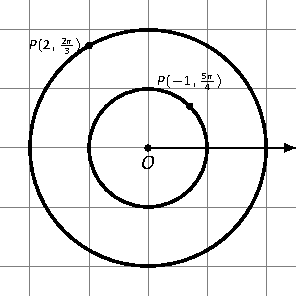
\includegraphics{figures/figpolar2}\\[5pt]
(a)\\[20pt]
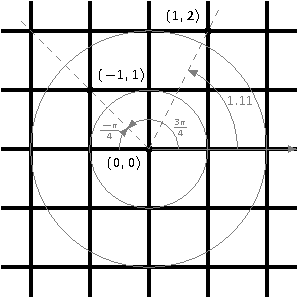
\includegraphics{figures/figpolar2b}\\[5pt]
(b)
\end{tabular}}	

\noindent\textbf{\large Polar Functions and Polar Graphs}\\

Defining a new coordinate system allows us to create a new kind of function, a \textbf{polar function.} Rectangular coordinates lent themselves well to creating functions that related $x$ and $y$, such as $y=x^2.$ Polar coordinates allow us to create functions that relate $r$ and $\theta$. Normally these functions look like $r=f(\theta)$, although we can create functions of the form $\theta = f(r)$. The following examples introduce us to this concept.\index{polar!functions}\index{polar!functions!graphing}\\

\example{ex_polar3}{Introduction to Graphing Polar Functions}{
Describe the graphs of the following polar functions.
\begin{enumerate}
	\item $r = 1.5$
	\item $\theta = \pi/4 $
\end{enumerate}
%
%\noindent$1.\ r = 1.5 \qquad 2.\ \theta = \pi/4 $
}
{\begin{enumerate}
\item The equation $r=1.5$ describes all points that are 1.5 units from the pole; as the angle is not specified, any $\theta$ is allowable. All points 1.5 units from the pole describes a circle of radius 1.5.

\mfigure{.25}{Plotting standard polar plots.}{fig:polar3}{figures/figpolar3}

We can consider the rectangular equivalent of this equation; using $r^2=x^2+y^2$, we see that $1.5^2=x^2+y^2$, which we recognize as the equation of a circle centered at $(0,0)$ with radius 1.5. This is sketched in Figure \ref{fig:polar3}.

\item The equation $\theta = \pi/4$ describes all points such that the line through them and the pole make an angle of $\pi/4$ with the initial ray. As the radius $r$ is not specified, it can be any value (even negative). Thus $\theta = \pi/4$ describes the line through the pole that makes an angle of $\pi/4 = 45^\circ$ with the initial ray: see Figure \ref{fig:polar3}.

We can again consider the rectangular equivalent of this equation. Combine $\tan \theta =y/x$ and $\theta =\pi/4$:
$$\tan \pi/4 = y/x \quad \Rightarrow x\tan \pi/4 = y \quad \Rightarrow y = x.$$ 
\end{enumerate}
\vskip-1.5\baselineskip
}\clearpage

The basic rectangular equations of the form $x=h$ and $y=k$ create vertical and horizontal lines, respectively; the basic polar equations $r= h$ and $\theta =\alpha$ create circles and lines through the pole, respectively. With this as a foundation, we can create more complicated polar functions of the form $r=f(\theta)$. The input is an angle; the output is a length, how far in the direction of the angle to go out.

We sketch these functions much like we sketch rectangular and parametric functions: we plot lots of points and ``connect the dots'' with curves. We demonstrate this in the following example.\\


\example{ex_polar4}{Sketching Polar Functions}{ 
Sketch the polar function $r=1+\cos \theta$ on $[0,2\pi]$ by plotting points.}
{A common question when sketching curves by plotting points is ``Which points should I plot?'' With rectangular equations, we often choose ``easy'' values -- integers, then added more if needed. When plotting polar equations, start with the ``common'' angles -- multiples of $\pi/6$ and $\pi/4$. Figure \ref{fig:polar4} gives a table of just a few values of $\theta$ in $[0,\pi]$. 

\mtable{.6}{Graphing a polar function in\\ Example \ref{ex_polar4} by plotting points.}{fig:polar4}{%
\begin{tabular}{c}
		$\begin{array}{cc}
		\theta & r=1+\cos\theta \\ \hline
 0 & 2 \\
 \pi/6 & 1.86603 \\
  \pi/2 & 1 \\
 4\pi/3 & 0.5 \\
 7 \pi /4 & 1.70711 \\
 \end{array}$\\
 \myincludegraphics[scale=0.9]{figures/figpolar4}
\end{tabular}}

Consider the point $P(0,2)$ determined by the first line of the table. The angle is 0 radians -- we do not rotate from the initial ray -- then we go out 2 units from the pole. When $\theta=\pi/6$, $r = 1.866$ (actually, it is $1+\sqrt{3}/2$); so rotate by $\pi/6$ radians and go out 1.866 units. 

The graph shown uses more points, connected with straight lines. (The points on the graph that correspond to points in the table are signified with larger dots.) Such a sketch is likely good enough to give one an idea of what the graph looks like.
}\\

\noindent\textbf{Technology Note:} Plotting functions in this way can be tedious, just as it was with rectangular functions. To obtain very accurate graphs, technology is a great aid. Most graphing calculators can plot polar functions; in the menu, set the plotting mode to something like \texttt{polar} or \texttt{POL}, depending on one's calculator. As with plotting parametric functions, the viewing ``window'' no longer determines the $x$-values that are plotted, so additional information needs to be provided. Often with the ``window'' settings are the settings for  the beginning and ending $\theta$ values (often called \texttt{$\theta_{\text{min}}$} and \texttt{$\theta_{\text{max}}$}) as well as the \texttt{$\theta_{\text{step}}$} -- that is, how far apart the $\theta$ values are spaced. The smaller the \texttt{$\theta_{\text{step}}$} value, the more accurate the graph (which also increases plotting time). Using technology, we graphed the polar function $r=1+\cos \theta$ from Example \ref{ex_polar4} in Figure \ref{fig:polar4b}.

\mfigure{.3}{Using  technology to graph a polar \\ function.}{fig:polar4b}{figures/figpolar4b}

\example{ex_polar5}{Sketching Polar Functions}{
Sketch the polar function $r=\cos (2\theta)$ on $[0,2\pi]$ by plotting points.}
{We start by making a table of $\cos (2\theta)$ evaluated at common angles $\theta$, as shown in Figure \ref{fig:polar5table}. These points are then plotted in Figure \ref{fig:polar5} (a). This particular graph ``moves'' around quite a bit and one can easily forget which points should be connected to each other. To help us with this, we numbered each point in the table and on the graph. 
%\clearpage

\begin{center}
\begin{minipage}[t]{125pt} \vskip0pt
$\begin{array}{ccc}
\text{Pt.} & \theta & \cos (2\theta)\\ \hline
 1 & 0 & 1. \\
 2 & \pi /6 & 0.5 \\
 3 & \pi /4 & 0. \\
 4 & \pi /3 & -0.5 \\
 5 & \pi /2 & -1. \\
 6 & 2 \pi /3 & -0.5 \\
 7 & 3 \pi /4 & 0. \\
 8 & 5 \pi /6 & 0.5 \\
 9 & \pi  & 1. \\
\end{array}$
\end{minipage}
\begin{minipage}[t]{125pt} \vskip 0pt
$\begin{array}{ccc}
\text{Pt.} & \theta & \cos (2\theta)\\ \hline
 10 & 7 \pi /6 & 0.5 \\
 11 & 5 \pi /4 & 0. \\
 12 & 4 \pi /3 & -0.5 \\
 13 & 3 \pi /2 & -1. \\
 14 & 5 \pi /3 & -0.5 \\
 15 & 7 \pi /4 & 0. \\
 16 & 11 \pi /6 & 0.5 \\
 17 & 2 \pi  & 1. \\
\end{array}$
\end{minipage}
\captionsetup{type=figure}
\caption{Tables of points for plotting a polar curve.}\label{fig:polar5table}
\end{center}
Using more points (and the aid of technology) a smoother plot can be made as shown in Figure \ref{fig:polar5} (b). This plot is an example of a \textit{rose curve}.
\mtable{.65}{Polar plots from Example \ref{ex_polar5}.}{fig:polar5}{%
\begin{tabular}{c}
\myincludegraphics{figures/figpolar5}\\[0pt]
(a) \\[0pt]
\myincludegraphics{figures/figpolar5b}\\[0pt]
(b) 
\end{tabular}
}
}\\

It is sometimes desirable to refer to a graph via a polar equation, and other times by a rectangular equation. Therefore it is necessary to be able to convert between polar and rectangular functions, which we practice in the following example. We will make frequent use of the identities found in Key Idea \ref{idea:polarconvert}.\\

\example{ex_polar6}{Converting between rectangular and polar equations.}{

\noindent
\begin{minipage}[t]{.5\linewidth}
Convert from rectangular to polar.
\begin{enumerate}
	\item $y=x^2$
	\item $xy = 1$
\end{enumerate}
\end{minipage}
\begin{minipage}[t]{.5\linewidth}
Convert from polar to rectangular.
\begin{enumerate}\addtocounter{enumi}{2}
	\item $\ds r=\frac{2}{\sin \theta-\cos\theta}$
	\item $r=2\cos \theta$
\end{enumerate}
\end{minipage}
}
{\begin{enumerate}
	\item Replace $y$ with $r\sin\theta$ and replace $x$ with $r\cos\theta$, giving:
	\begin{align*}
	y &=x^2\\
	r\sin\theta &= r^2\cos^2\theta\\
	\frac{\sin\theta}{\cos^2\theta} &= r
	\end{align*}
	We have found that $r=\sin\theta/\cos^2\theta = \tan\theta\sec\theta$. The domain of this polar function is $(-\pi/2,\pi/2)$; plot a few points to see how the familiar parabola is traced out by the polar equation.
	
	\item		We again replace $x$ and $y$ using the standard identities and work to solve for $r$:
	\begin{align*}
	xy &= 1 \\
	r\cos\theta\cdot r\sin\theta & = 1\\
	r^2 & = \frac{1}{\cos\theta\sin\theta}\\
	r & = \frac{1}{\sqrt{\cos\theta\sin\theta}}\\
	\end{align*}
	This function is valid only when the product of $\cos\theta\sin\theta$ is positive. This occurs in the first and third quadrants, meaning the domain of this polar function is $(0,\pi/2) \cup (\pi,3\pi/2)$.
	
	We can rewrite the original rectangular equation $xy=1$ as $y=1/x$. This is graphed in Figure \ref{fig:polar6}; note how it only exists in the first and third quadrants.
	\mfigure{.25}{Graphing $xy=1$ from Example \ref{ex_polar6}.}{fig:polar6}{figures/figpolar6}
		
	\item		There is no set way to convert from polar to rectangular; in general, we look to form the products $r\cos \theta$ and $r\sin\theta$, and then replace these with $x$ and $y$, respectively. We start in this problem by multiplying both sides by $\sin\theta-\cos\theta$:
	\begin{align*}
	r &= \frac{2}{\sin\theta-\cos\theta} \\
	r(\sin\theta-\cos\theta) &= 2\\
	r\sin\theta-r\cos\theta &= 2. \qquad \text{Now replace with $y$ and $x$:}\\
	y-x &= 2\\
	y &= x+2.
	\end{align*}
	The original polar equation, $r=2/(\sin\theta-\cos\theta)$ does not easily reveal that its graph is simply a line. However, our conversion shows that it is. The upcoming gallery of polar curves gives the general equations of lines in polar form.

\drawexampleline
	
	\item		By multiplying both sides by $r$, we obtain both an $r^2$ term and an $r\cos\theta$ term, which we replace with $x^2+y^2$ and $x$, respectively. 
	\begin{align*}
	r &=2\cos\theta \\
	r^2 &= 2r\cos\theta \\
	x^2+y^2 &= 2x. 
	\intertext{We recognize this as a circle; by completing the square we can find its radius and center.}
	x^2-2x+y^2 &= 0 \\
	(x-1)^2 + y^2 &=1.
	\end{align*}
	The circle is centered at $(1,0)$ and has radius 1. The upcoming gallery of polar curves gives the equations of \textit{some} circles in polar form; circles with arbitrary centers have a complicated polar equation that we do not consider here.
	\end{enumerate}
	\vskip-\baselineskip
}\\

Some curves have very simple polar equations but rather complicated rectangular ones. For instance, the equation $r=1+\cos\theta$ describes a \textit{cardiod} (a shape important the sensitivity of microphones, among other things; one is graphed in the gallery in the Lima\c con section). It's rectangular form is not nearly as simple; it is the implicit equation
$x^4+y^4+2x^2y^2-2xy^2-2x^3-y^2=0.$ The conversion is not ``hard,'' but takes several steps, and is left as a problem in the Exercise section.\\
\pagebreak

\noindent\textbf{\Large Gallery of Polar Curves}\\

There are a number of basic and ``classic'' polar curves, famous for their beauty and/or applicability to the sciences. \index{polar!function!gallery of graphs} This section ends with a small gallery of some of these graphs. We encourage the reader to understand how these graphs are formed, and to investigate with technology other types of polar functions.\\

\enlargethispage{2\baselineskip}
\newlength{\gallerywidth}
\setlength{\gallerywidth}{(0pt+\marginparwidth+\textwidth)/4}
\vskip \baselineskip
\noindent%\hskip-\marginparwidth%\hskip-25pt
\rule{25pt+\marginparwidth+\textwidth}{1pt}\\

\noindent%\hskip-\marginparwidth\hskip-25pt
\textbf{\large Lines}\\

\noindent%\hskip-\marginparwidth\hskip-30pt
\begin{tabular}{p{\gallerywidth}p{\gallerywidth}p{\gallerywidth}p{\gallerywidth}}
\textbf{Through the origin:} & \textbf{Horizontal line:} & \textbf{Vertical line:} & \textbf{Not through origin:} \\[5pt]
$\theta = \alpha$ & $r=a\csc\theta$ & $r=a\sec\theta$ & $\ds r=\frac{b}{\sin\theta-m\cos\theta}$ \\[10pt]
\myincludegraphics[scale=.9]{figures/figpolarline1} & \myincludegraphics[scale=.9]{figures/figpolarline2} & \myincludegraphics[scale=.9]{figures/figpolarline4} & \myincludegraphics[scale=.9]{figures/figpolarline3}
\end{tabular}

%\clearpage\exercisegeometry\exerciseheader
%\ \vskip0pt
%\vskip-.25in
\noindent\parbox{3\gallerywidth+37pt}{\textbf{\large Circles}}\textbf{\large Spiral}\\

\noindent\hskip-5pt%
\begin{tabular}{p{\gallerywidth}p{\gallerywidth}p{\gallerywidth}p{\gallerywidth}}
\textbf{Centered on $x$-axis:} & \textbf{Centered on $y$-axis:} & \textbf{Centered on origin:} &\textbf{Archimedean spiral}\\
$r=a\cos \theta$ & $r=a\sin\theta$ & $r=a$ & $r=\theta$\\
\myincludegraphics[scale=.9]{figures/figpolarcircle1}&\myincludegraphics[scale=.9]{figures/figpolarcircle2}&\myincludegraphics[scale=.9]{figures/figpolarcircle3}&\myincludegraphics[scale=.9]{figures/figpolarspiral}
\end{tabular}\\

\pagebreak

\noindent\hskip-\marginparwidth\hskip-25pt\textbf{\large Lima\c cons}\\

\noindent\hskip-\marginparwidth\hskip-25pt%
\begin{tabular}{p{\gallerywidth}p{\gallerywidth}p{\gallerywidth}p{\gallerywidth}}
\multicolumn{4}{l}{Symmetric about $x$-axis: $r=a\pm b\cos\theta$; \quad Symmetric about $y$-axis:  $r=a\pm b\sin \theta$; \quad $a,b>0$}\\
\\
\textbf{With inner loop:} & \textbf{Cardiod:} & \textbf{Dimpled:} & \textbf{Convex:} \\[5pt]
$\ds \frac ab < 1$ & $\ds \frac ab=1$ & $\ds 1<\frac ab <2$ & $\ds \frac ab>2$ \\[10pt]
\myincludegraphics[scale=.9]{figures/figpolarlimacon1} & \myincludegraphics[scale=.9]{figures/figpolarlimacon2} & \myincludegraphics[scale=.9]{figures/figpolarlimacon3} & \myincludegraphics[scale=.9]{figures/figpolarlimacon4}
\end{tabular}\\

\noindent\hskip-\marginparwidth\hskip-25pt\textbf{\large Rose Curves}\\

\enlargethispage{20\baselineskip}
\noindent\hskip-\marginparwidth\hskip-25pt
\begin{tabular}{p{\gallerywidth}p{\gallerywidth}p{\gallerywidth}p{\gallerywidth}}
\multicolumn{4}{l}{Symmetric about $x$-axis: $r=a \cos(n\theta)$; \quad Symmetric about $y$-axis:  $r=a\sin(n\theta)$}\\
\multicolumn{4}{l}{Curve contains $2n$ petals when $n$ is even and $n$ petals when $n$ is odd.}\\
\\
%\textbf{With inner loop:} & \textbf{Cardiod:} & \textbf{Dimpled:} & \textbf{Convex:} \\[5pt]
$r=a\cos (2\theta)$ & $r=a\sin(2\theta)$ & $r=a\cos (3\theta)$ & $r=a\sin (3\theta)$ \\[10pt]
\myincludegraphics[scale=.9]{figures/figpolarrose1} & \myincludegraphics[scale=.9]{figures/figpolarrose2} & \myincludegraphics[scale=.9]{figures/figpolarrose4} & \myincludegraphics[scale=.9]{figures/figpolarrose3}
\end{tabular}\\
%\clearpage

\noindent\hskip-\marginparwidth\hskip-25pt
\textbf{\large Special Curves}\\

\noindent\hskip-5pt\hskip-\marginparwidth\hskip-25pt%
\begin{tabular}{p{\gallerywidth}p{\gallerywidth}p{\gallerywidth}p{\gallerywidth}}
\textbf{Rose curves} &  & \textbf{Lemniscate:} & \textbf{Eight Curve:} \\[5pt]
$r=a\sin (\theta/5)$ & $r=a\sin(2\theta/5)$ & $r^2=a^2\cos (2\theta)$ & $r^2=a^2\sec^4\theta\cos (2\theta)$ \\[10pt]
\myincludegraphics[scale=.9]{figures/figpolarspecial1} & \myincludegraphics[scale=.9]{figures/figpolarspecial2} & \myincludegraphics[scale=.9]{figures/figpolarspecial3} & \myincludegraphics[scale=.9]{figures/figpolarspecial4}
\end{tabular}\\

\restoregeometry
\regularheader
\pagebreak
%\clearpage

Earlier we discussed how each point in the plane does not have a unique representation in polar form. This can be a ``good'' thing, as it allows for the beautiful and interesting curves seen in the preceding gallery. However, it can also be a ``bad'' thing, as it can be difficult to determine where two curves intersect.\\

\example{ex_polar7}{Finding points of intersection with polar curves}{
Determine where the graphs of the polar equations $r=1+3\cos\theta$ and $r=\cos \theta$ intersect.
}
{As technology is generally readily available, it is usually a good idea to start with a graph. We have graphed the two functions in Figure \ref{fig:polar7}(a); to better discern the intersection points, part (b) of the figure zooms in around the origin.
\mtable{.5}{Graphs to help determine the points of intersection of the polar functions given in Example \ref{ex_polar7}.}{fig:polar7}{%
\begin{tabular}{c}
\myincludegraphics{figures/figpolar7}\\
(a)\\[10pt]
\myincludegraphics{figures/figpolar7b}\\
(b)
\end{tabular}
}
We start by setting the two functions equal to each other and solving for $\theta$:
\begin{align*}
1+3\cos\theta &= \cos \theta \\
2\cos\theta &= -1\\
\cos\theta&= -\frac12\\
\theta &= \frac{2\pi}{3}, \frac{4\pi}{3}.
\end{align*}
(There are, of course, infinite solutions to the equation $\cos\theta=-1/2$; as the lima\c con is traced out once on $[0,2\pi]$, we restrict our solutions to this interval.) 

We need to analyze this solution. When $\theta = 2\pi/3$ we obtain the point of intersection that lies in the 4$^\text{th}$ quadrant. When $\theta = 4\pi/3$, we get the point of intersection that lies in the 2$^\text{nd}$ quadrant. There is more to say about this second intersection point, however. The circle defined by $r=\cos\theta$ is traced out once on $[0,\pi]$, meaning that this point of intersection occurs while tracing out the circle a second time. It seems strange to pass by the point once and then recognize it as a point of intersection only when arriving there a ``second time.'' The first time the circle arrives at this point is when $\theta = \pi/3$.
It is key to understand that these two points are the same: $(\cos \pi/3,\pi/3)$ and $(\cos 4\pi/3,4\pi/3)$. 

To summarize what we have done so far, we have found two points of intersection: when $\theta=2\pi/3$ and when $\theta=4\pi/3$. When referencing the circle $r=\cos \theta$, the latter point is better referenced as when $\theta=\pi/3$.

There is yet another point of intersection: the pole (or, the origin). We did not recognize this intersection point using our work above as each graph arrives at the pole at a different $\theta$ value.

A graph intersects the pole when $r=0$. Considering the circle $r=\cos\theta$, $r=0$ when $\theta = \pi/2$ (and odd multiples thereof, as the circle is repeatedly traced). The lima\c con intersects the pole when $1+3\cos\theta =0$; this occurs when $\cos \theta = -1/3$, or for $\theta = \cos^{-1}(-1/3)$. This is a nonstandard angle, approximately $\theta = 1.9106 = 109.47^\circ$. The lima\c con intersects the pole twice in $[0,2\pi]$; the other angle at which the lima\c con is at the pole is the reflection of the first angle across the $x$-axis. That is, $\theta = 4.3726 = 250.53^\circ.$
}\\

If all one is concerned with is the $(x,y)$ coordinates at which the graphs intersect, much of the above work is extraneous. We know they intersect at $(0,0)$; we might not care at what $\theta$ value. Likewise, using $\theta =2\pi/3$ and $\theta=4\pi/3$ can give us the needed rectangular coordinates. However, in the next section we apply calculus concepts to polar functions. When computing the area of a region bounded by polar curves, understanding the nuances of the points of intersection becomes important.

\printexercises{exercises/09_04_exercises}

\section{Calculus and Polar Functions} \label{sec:polarcalc}
The previous section defined polar coordinates, leading to polar functions. We investigated plotting these functions and solving a fundamental question about their graphs, namely, where do two polar graphs intersect?

We now turn our attention to answering other questions, whose solutions require the use of calculus. A basis for much of what is done in this section is the ability to turn a polar function $r=f(\theta)$ into a set of parametric equations. Using the identities $x=r\cos \theta$ and $y=r\sin \theta$, we can create the parametric equations $x=f(\theta)\cos\theta$, $y=f(\theta)\sin\theta$ and apply the concepts of Section \ref{sec:par_calc}.\\

\noindent\textbf{\large Polar Functions and $\ds \frac{dy}{dx}$}\\

We are interested in the lines tangent a given graph, regardless of whether that graph is produced by rectangular, parametric, or polar equations. In each of these contexts, the slope of the tangent line is $\frac{dy}{dx}$. Given $r=f(\theta)$, we are generally \textit{not} concerned with $r\,'=\fp(\theta)$; that describes how fast $r$ changes with respect to $\theta$. Instead, we will use $x=f(\theta)\cos\theta$, $y=f(\theta)\sin\theta$ to compute $\frac{dy}{dx}$. 

Using Key Idea \ref{idea:dydxpar} we have $$\frac{dy}{dx} = \frac{dy}{d\theta}\Big/\frac{dx}{d\theta}.$$ Each of the two derivatives on the right hand side of the equality requires the use of the Product Rule. We state the important result as a Key Idea.\\

\keyidea{idea:dydxpol}{Finding $\frac{dy}{dx}$ with Polar Functions}
{Let $r=f(\theta)$ be a polar function. With $x=f(\theta)\cos\theta$ and $y=f(\theta)\sin\theta$,
\index{polar!functions!finding $\frac{dy}{dx}$}\index{tangent line}
$$\frac{dy}{dx} = \frac{\fp(\theta)\sin\theta+f(\theta)\cos\theta}{\fp(\theta)\cos\theta-f(\theta)\sin\theta}.$$
}

\example{ex_polcalc1}{Finding $\frac{dy}{dx}$ with polar functions.}
{Consider the lima\c con $r=1+2\sin\theta$ on $[0,2\pi]$.
\begin{enumerate}
	\item Find the equations of the tangent and normal lines to the graph at $\theta=\pi/4$.
	\item		Find where the graph has vertical and horizontal tangent lines.
\end{enumerate}
}
{\begin{enumerate}
	\item We start by computing $\frac{dy}{dx}$. With $\fp(\theta) = 2\cos\theta$, we have
	\begin{align*}
	\frac{dy}{dx} &= \frac{2\cos\theta\sin\theta + \cos\theta(1+2\sin\theta)}{2\cos^2\theta-\sin\theta(1+2\sin\theta)}\\
	&= \frac{\cos\theta(4\sin\theta+1)}{2(\cos^2\theta-\sin^2\theta)-\sin\theta}.
	\end{align*}
	When $\theta=\pi/4$, $\frac{dy}{dx}=-2\sqrt{2}-1$ (this requires a bit of simplification). In rectangular coordinates, the point on the graph at $\theta=\pi/4$ is $(1+\sqrt{2}/2,1+\sqrt{2}/2)$. Thus the rectangular equation of the line tangent to the lima\c con at $\theta=\pi/4$ is 
	$$y=(-2\sqrt{2}-1)\big(x-(1+\sqrt{2}/2)\big)+1+\sqrt{2}/2 \approx  -3.83 x+8.24.$$ The lima\c con and the tangent line are graphed in Figure \ref{fig:polcalc1}. 
	
	The normal line has the opposite--reciprocal slope as the tangent line, so its equation is 
	$$y \approx \frac{1}{3.83}x+1.26.$$
	\mfigure{.75}{The lima\c con in Example \ref{ex_polcalc1} with its tangent line at $\theta=\pi/4$ and points of vertical and horizontal tangency.}{fig:polcalc1}{figures/figpolcalc1}
	\drawexampleline
	
	\item		To find the horizontal lines of tangency, we find where $\frac{dy}{dx}=0$; thus we find where the numerator of our equation for $\frac{dy}{dx}$ is 0.
	$$\cos\theta(4\sin\theta+1)=0\quad \Rightarrow \quad \cos\theta=0 \quad \text{or}\quad 4\sin\theta+1=0.$$
	On $[0,2\pi]$, $\cos\theta=0$ when $\theta=\pi/2,\ 3\pi/2$. 

Setting $4\sin\theta+1=0$ gives $\theta=\sin^{-1}(-1/4)\approx -0.2527 = -14.48^\circ$. We want the results in $[0,2\pi]$; we also recognize there are two solutions, one in the 3$^\text{rd}$ quadrant and one in the 4$^\text{th}$. Using reference angles, we have our two solutions as $\theta =3.39$ and $6.03$ radians. The four points we obtained where the lima\c con has a horizontal tangent line are given in Figure \ref{fig:polcalc1} with black--filled dots.\\

To find the vertical lines of tangency, we set the denominator of $\frac{dy}{dx}=0$. 
\begin{align*}
2(\cos^2\theta -\sin^2\theta)-\sin\theta &= 0 .
\intertext{Convert the $\cos^2\theta$ term to $1-\sin^2\theta$:}
2(1-\sin^2\theta-\sin^2\theta)-\sin\theta &= 0\\
4\sin^2\theta + \sin\theta -1 &= 0.
\intertext{Recognize this as a quadratic in the variable $\sin\theta$. Using the quadratic formula, we have}
\sin\theta &= \frac{-1\pm\sqrt{33}}{8}.
\end{align*}
We solve $\sin\theta = \frac{-1+\sqrt{33}}8$ and $\sin\theta = \frac{-1-\sqrt{33}}8$:
\begin{align*}
\sin\theta &=\frac{-1+\sqrt{33}}8 & \sin\theta &= \frac{-1-\sqrt{33}}{8}\\
\theta &= \sin^{-1}\left(\frac{-1+\sqrt{33}}8\right) & \theta &= \sin^{-1}\left(\frac{-1-\sqrt{33}}8\right)\\
\theta &= 0.6399 & \theta &= -1.0030
\end{align*}
In each of the solutions above, we only get one of the possible two solutions as $\sin^{-1}x$ only returns solutions in $[-\pi/2,\pi/2]$, the 4$^\text{th}$ and $1^\text{st}$ quadrants. Again using reference angles, we have:
$$\sin\theta = \frac{-1+\sqrt{33}}8 \quad \Rightarrow \quad \theta = 0.6399,\ 3.7815 \text{ radians}$$
and 
$$\sin\theta = \frac{-1-\sqrt{33}}8 \quad \Rightarrow \quad \theta = 4.1446,\ 5.2802 \text{ radians.}$$
These points are also shown in Figure \ref{fig:polcalc1} with white--filled dots.
	\end{enumerate}
	\vskip-\baselineskip
}\\

When the graph of the polar function $r=f(\theta)$ intersects the pole, it means that $f(\alpha)=0$ for some angle $\alpha$. Thus the formula for $\frac{dy}{dx}$ in such instances is very simple, reducing simply to $$\frac{dy}{dx} = \tan \alpha.$$
This equation makes an interesting point. It tells us the slope of the tangent line at the pole is $\tan \alpha$; some of our previous work (see, for instance, Example \ref{ex_polar3}) shows us that the line through the pole with slope $\tan \alpha$ has polar equation $\theta=\alpha$. Thus when a polar graph touches the pole at $\theta=\alpha$, the equation of the tangent line at the pole is $\theta=\alpha$. \\

\example{ex_polcalc2}{Finding tangent lines at the pole.}{
Let $r=1+2\sin\theta$, a lima\c con. Find the equations of the lines tangent to the graph at the pole.
\mfigure{.55}{Graphing the tangent lines at the pole in Example \ref{ex_polcalc2}.}{fig:polcalc2}{figures/figpolcalc2}}
{We need to know when $r=0$. 
\begin{align*}
1+2\sin\theta &= 0\\
\sin\theta &= -1/2\\
\theta &= \frac{7\pi}{6},\ \frac{11\pi}6.
\end{align*}
Thus the equations of the tangent lines, in polar, are $\theta = 7\pi/6$ and $\theta = 11\pi/6$. In rectangular form, the tangent lines are $y=\tan(7\pi/6)x$ and $y=\tan(11\pi/6)x$. The full lima\c con can be seen in Figure \ref{fig:polcalc1}; we zoom in on the tangent lines in Figure \ref{fig:polcalc2}.
}\\

\noindent\textbf{\large Area}\\

When using rectangular coordinates, the equations $x=h$ and $y=k$ defined vertical and horzontal lines, respectively, and combinations of these lines create rectangles (hence the name ``rectangular coordinates''). It is then somewhat natural to use rectangles to approximate area as we did when learning about the definite integral.\index{polar!functions!area}

When using polar coordinates, the equations $\theta=\alpha$ and $r=c$ form lines through the origin and circles centered at the origin, respectively, and combinations of these curves form sectors of circles. It is then somewhat natural to calculate the area of regions defined by polar functions by first approximating with sectors of circles. 

Consider Figure \ref{fig:polararea} (a) where a region defined by $r=f(\theta)$ on $[\alpha,\beta]$ is given. (Note how the ``sides'' of the region are the lines $\theta=\alpha$ and $\theta=\beta$, whereas in rectangular coordinates the ``sides'' of regions were often the vertical lines $x=a$ and $x=b$.)
\mnote{.3}{\textbf{Note:} Recall that the area of a sector of a circle with radius $r$ subtended by an angle $\theta$ is $A = \frac12\theta r^2$.

\hfill
\begin{tikzpicture}[x=30pt,y=30pt,thick]
			\draw (2,0) arc (0:50:2) -- (0,0);
			\draw [] (0,0) -- (2,0) node [pos=.5,below] {$r$};
			\draw [fill=black] (0,0) circle (1pt);
			%\draw (1.95,1.0) node {$s$};
			\draw (0,0) node [shift={(15pt,8pt)}] {$\theta$};
			\end{tikzpicture}
\hfill\null
}

Partition the interval $[\alpha,\beta]$ into $n$ equally spaced subintervals as $\alpha = \theta_1 < \theta_2 <\cdots <\theta_{n+1}=\beta$. The length of each subinterval is $\Delta\theta = (\beta-\alpha)/n$, representing a small change in angle. The area of the region defined by the $i\,^\text{th}$ subinterval $[\theta_i,\theta_{i+1}]$ can be approximated with a sector of a circle with radius $f(c_i)$, for some $c_i$ in $[\theta_i,\theta_{i+1}]$. The area of this sector is $\frac12f(c_i)^2\Delta\theta$. This is shown in part (b) of the figure, where $[\alpha,\beta]$ has been divided into 4 subintervals. We approximate the area of the whole region by summing the areas of all sectors:
$$\text{Area} \approx \sum_{i=1}^n \frac12f(c_i)^2\Delta\theta.$$
This is a Riemann sum. By taking the limit of the sum as $n\to\infty$, we find the exact area of the region in the form of a definite integral.
\mtable{.7}{Computing the area of a polar region.}{fig:polararea}{%
\begin{tabular}{c}
\myincludegraphics{figures/figpolarea1}\\
(a)\\[10pt]
\myincludegraphics{figures/figpolarea2}\\
(b)
\end{tabular}
}
\enlargethispage{2\baselineskip}
%\clearpage

\theorem{thm:polar_area}{Area of a Polar Region}
{Let $f$ be continuous and non-negative on $[\alpha,\beta]$, where $0\leq \beta-\alpha\leq 2\pi$. The area  $A$ of the region bounded by the curve $r=f(\theta)$ and the lines $\theta=\alpha$ and $\theta=\beta$ is 
$$
A \ =\  \frac12\int_\alpha^\beta f(\theta)^2 \ d\theta\  =\  \frac12\int_\alpha^\beta r^{\,2} \ d\theta$$
}

The theorem states that $0\leq \beta-\alpha\leq 2\pi$. This ensures that region does not overlap itself, which would give a result that does not correspond directly to the area.\\

%\pagebreak

\example{ex_polcalc3}{Area of a polar region}{
Find the area of the circle defined by $r=\cos \theta$. (Recall this circle has radius $1/2$.)}
{This is a direct application of Theorem \ref{thm:polar_area}. The circle is traced out on $[0,\pi]$, leading to the integral
\begin{align*}
\text{Area} &= \frac12\int_0^\pi \cos^2\theta\ d  \theta \\
						&= \frac12\int_0^\pi \frac{1+\cos(2\theta)}{2}\ d\theta\\
						&= \frac14\big(\theta +\frac12\sin(2\theta)\big)\Bigg|_0^\pi\\
						&= \frac14\pi.
\end{align*}
Of course, we already knew the area of a circle with radius $1/2$. We did this example to demonstrate that the area formula is correct.
}\\

\mnote{.3}{\textbf{Note:} Example \ref{ex_polcalc3} requires the use of the integral $\ds\int \cos^2\theta\ d\theta$. This is handled well by using the power reducing formula as found in the back of this text. Due to the nature of the area formula, integrating $\cos^2\theta$ and $\sin^2\theta$ is required often. We offer here these indefinite integrals as a time--saving measure.\\
$$\int\cos^2\theta\ d\theta = \frac12\theta+\frac14\sin(2\theta)+C$$
$$\int\sin^2\theta\ d\theta = \frac12\theta-\frac14\sin(2\theta)+C$$
}
\pagebreak

\example{ex_polcalc4}{Area of a polar region}{
Find the area of the cardiod $r=1+\cos\theta$ bound between $\theta=\pi/6$ and $\theta=\pi/3$, as shown in Figure \ref{fig:polcalc4}.
}
{This is again a direct application of Theorem \ref{thm:polar_area}. 
\begin{align*}
\text{Area} &= \frac12\int_{\pi/6}^{\pi/3} (1+\cos\theta)^2\ d\theta\\
				&= \frac12\int_{\pi/6}^{\pi/3} (1+2\cos\theta+\cos^2\theta)\ d\theta\\
				&= \frac12\left(\theta+2\sin\theta+\frac12\theta+\frac14\sin(2\theta)\right)\Bigg|_{\pi/6}^{\pi/3} \\
				&= \frac18\big(\pi+4\sqrt{3}-4\big) \approx 0.7587.
				\end{align*}
\vskip-\baselineskip
}\\

\mfigure{.8}{Finding the area of the shaded region of a cardiod in Example \ref{ex_polcalc4}.}{fig:polcalc4}{figures/figpolcalc4}

\noindent\textbf{Area Between Curves}\\

Our study of area in the context of rectangular functions led naturally to finding area bounded between curves. We consider the same in the context of polar functions. \index{polar!functions!area between curves}

Consider the shaded region shown in Figure \ref{fig:polarea3}. We can find the area of this region by computing the area bounded by $r_2=f_2(\theta)$ and subtracting the area bounded by $r_1=f_1(\theta)$ on $[\alpha,\beta]$. Thus
$$\text{Area}\ = \ \frac12\int_\alpha^\beta r_2^{\,2}\ d\theta - \frac12\int_\alpha^\beta r_1^{\,2}\ d\theta = \frac12\int_\alpha^\beta \big(r_2^{\,2}-r_1^{\,2}\big)\ d\theta.$$
\mfigure{.5}{Illustrating area bound between two polar curves.}{fig:polarea3}{figures/figpolarea3}

\keyidea{idea:area_between_polar}{Area Between Polar Curves}
{The area $A$ of the region bounded by $r_1=f_1(\theta)$ and $r_2=f_2(\theta)$, $\theta=\alpha$ and $\theta=\beta$, where $f_1(\theta)\leq f_2(\theta)$ on $[\alpha,\beta]$, is
$$A = \frac12\int_\alpha^\beta \big(r_2^{\,2}-r_1^{\,2}\big)\ d\theta.$$
}

\enlargethispage{2\baselineskip}
\example{ex_polcalc5}{Area between polar curves}{
Find the area bounded between the curves $r=1+\cos \theta$ and $r=3\cos\theta$, as shown in Figure \ref{fig:polcalc5}.
\mfigure{.25}{Finding the area between polar curves in Example \ref{ex_polcalc5}.}{fig:polcalc5}{figures/figpolcalc5}
}
{We need to find the points of intersection between these two functions. Setting them equal to each other, we find:
\begin{align*}
1+\cos\theta &= 3\cos \theta \\
 \cos\theta &=1/2\\
\theta &= \pm \pi/3
\end{align*}
Thus we integrate $\frac12\big((3\cos\theta)^2-(1+\cos\theta)^2\big)$ on $[-\pi/3,\pi/3]$.
\begin{align*}
\text{Area} &= \frac12\int_{-\pi/3}^{\pi/3} \big((3\cos\theta)^2-(1+\cos\theta)^2\big)\ d\theta\\
		&= \frac12\int_{-\pi/3}^{\pi/3} \big( 8\cos^2\theta-2\cos\theta-1\big)\ d\theta \\
		&= \big(2\sin(2\theta) - 2\sin\theta+3\theta\big)\Bigg|_{-\pi/3}^{\pi/3}\\
		&= 2\pi.
\end{align*}
Amazingly enough, the area between these curves has a ``nice'' value.
}\\

\example{ex_polcalc6}{Area defined by polar curves}{
Find the area bounded between the polar curves $r=1$ and $r=2\cos(2\theta)$, as shown in Figure \ref{fig:polcalc6} (a).}
{We need to find the point of intersection between the two curves. Setting the two functions equal to each other, we have
$$2\cos(2\theta) = 1 \quad \Rightarrow \quad \cos(2\theta) = \frac12 \quad \Rightarrow \quad 2\theta = \pi/3\quad \Rightarrow \quad \theta=\pi/6.$$
\mtable{.6}{Graphing the region bounded by the functions in Example \ref{ex_polcalc6}.}{fig:polcalc6}{%
\begin{tabular}{c}
\myincludegraphics{figures/figpolcalc6}\\
(a)\\[10pt]
\myincludegraphics{figures/figpolcalc6a}\\
(b)\\
\end{tabular}
}
In part (b) of the figure, we zoom in on the region and note that it is not really bounded \textit{between} two polar curves, but rather \textit{by} two polar curves, along with $\theta=0$. The dashed line breaks the region into its component parts. Below the dashed line, the region is defined by $r=1$, $\theta=0$ and $\theta = \pi/6$. (Note: the dashed line lies on the line $\theta=\pi/6$.) Above the dashed line the region is bounded by $r=2\cos(2\theta)$ and $\theta =\pi/6$. Since we have two separate regions, we find the area using two separate integrals.

Call the area below the dashed line $A_1$ and the area above the dashed line $A_2$. They are determined by the following integrals:
$$A_1 = \frac12\int_0^{\pi/6} (1)^2\ d\theta\qquad  A_2 = \frac12\int_{\pi/6}^{\pi/4} \big(2\cos(2\theta)\big)^2\ d\theta.$$
(The upper bound of the integral computing $A_2$ is $\pi/4$ as $r=2\cos(2\theta)$ is at the pole when $\theta=\pi/4$.)

We omit the integration details and let the reader verify that $A_1 = \pi/12$ and $A_2 = \pi/12-\sqrt{3}/8$; the total area is $A = \pi/6-\sqrt{3}/8$.
}\\

\noindent\textbf{\large Arc Length}\\

As we have already considered the arc length of curves defined by rectangular and parametric equations, we now consider it in the context of polar equations. Recall that the arc length $L$ of the graph defined by the parametric equations $x=f(t)$, $y=g(t)$ on $[a,b]$ is
\index{arc length}\index{polar!function!arc length}
\begin{equation}L = \int_a^b \sqrt{\fp(t)^2 + g\primeskip'(t)^2}\ dt = \int_a^b \sqrt{x\primeskip'(t)^2+y\primeskip'(t)^2}\ dt.\label{eq:polar_arclength}\end{equation}

Now consider the polar function $r=f(\theta)$. We again use the identities $x=f(\theta)\cos\theta$ and $y=f(\theta)\sin\theta$ to create parametric equations based on the polar function. We compute $x\primeskip'(\theta)$ and $y\primeskip'(\theta)$ as done before when computing $\frac{dy}{dx}$, then apply Equation \eqref{eq:polar_arclength}.

The expression $x\primeskip'(\theta)^2+y\primeskip'(\theta)^2$ can be simplified a great deal; we leave this as an exercise and state that $$x\primeskip'(\theta)^2+y\primeskip'(\theta)^2 = \fp(\theta)^2+f(\theta)^2.$$ This leads us to the  arc length formula.

\keyidea{idea:polar_arclength}{Arc Length of Polar Curves}
{Let  $r=f(\theta)$ be a polar function with $\fp$ continuous on an open interval $I$ containing $[\alpha,\beta]$, on which the graph traces itself only once. The arc length $L$ of the graph on $[\alpha,\beta]$ is
$$L = \int_\alpha^\beta \sqrt{\fp(\theta)^2+f(\theta)^2}\ d\theta = \int_\alpha^\beta\sqrt{(r\,')^2+ r^2}\ d\theta.$$
}

\example{ex_polcalc7}{Arc length of a lima\c con}{
Find the arc length of the lima\c con $r=1+2\sin t$.}
{With $r=1+2\sin t$, we have $r\,' = 2\cos t$. The lima\c con is traced out once on $[0,2\pi]$, giving us our bounds of integration. Applying Key Idea \ref{idea:polar_arclength}, we have
\begin{align*}
L 	&= \int_0^{2\pi} \sqrt{(2\cos\theta)^2+(1+2\sin\theta)^2}\ d\theta \\
		&=	\int_0^{2\pi} \sqrt{4\cos^2\theta+4\sin^2\theta +4\sin\theta+1}\ d\theta\\
		&=	\int_0^{2\pi} \sqrt{4\sin\theta+5}\ d\theta\\
		&\approx 13.3649.
\end{align*}
\mfigure{.45}{The lima\c con in Example \ref{ex_polcalc7} whose arc length is measured.}{fig:polcalc7}{figures/figpolcalc7}
The final integral cannot be solved in terms of elementary functions, so we resorted to a numerical approximation. (Simpson's Rule, with $n=4$, approximates the value with $13.0608$. Using $n=22$ gives the value above, which is accurate to 4 places after the decimal.) 
}\\
\pagebreak

\noindent\textbf{\large Surface Area}\\

The formula for arc length leads us to a formula for surface area. The following Key Idea is based on Key Idea \ref{idea:surface_area_parametric}.

\keyidea{idea:surface_area_polar}{Surface Area of a Solid of Revolution}
{Consider the graph of the polar equation $r=f(\theta)$, where $\fp$ is continuous on an open interval containing $[\alpha,\beta]$ on which the graph does not cross itself.
\index{surface area!solid of revolution}\index{polar!function!surface area}\index{integration!surface area}
	\begin{enumerate}
		\item The surface area of the solid formed by revolving the graph about the initial ray ($\theta=0$) is:
		$$\text{Surface Area} = 2\pi\int_\alpha^\beta f(\theta)\sin\theta\sqrt{\fp(\theta)^2+f(\theta)^2}\ d\theta.$$
		\item The surface area of the solid formed by revolving the graph about the line $\theta=\pi/2$ is:
		$$\text{Surface Area} = 2\pi\int_\alpha^\beta f(\theta)\cos\theta\sqrt{\fp(\theta)^2+f(\theta)^2}\ d\theta.$$
	\end{enumerate}
}
%\clearpage

\example{ex_polcalc8}{Surface area determined by a polar curve}{
Find the surface area formed by revolving one petal of the rose curve $r=\cos(2\theta)$ about its central axis (see Figure \ref{fig:polcalc8}).}
{\mtable{.4}{Finding the surface area of a rose--curve petal that is revolved around its central axis.}{fig:polcalc8}{%
\begin{tabular}{c}
\myincludegraphics{figures/figpolcalc8}\\
(a)\\[10pt]
%%\ifthenelse{\boolean{in_threeD}}{{%
%%\myincludegraphicsthree[width=150pt,3Dmenu,activate=onclick,deactivate=pageinvisible,
%%3Droll=0,
%%3Dortho=0.009,
%%3Dc2c=0.41893383860588074 -0.887881875038147 0.1901581883430481,
%%3Dcoo=65.85308837890625 6.341495513916016 17.98039436340332,
%%3Droo=85,
%%3Dlights=Headlamp,add3Djscript=asylabels.js]{figures/figpolcalc8a_3D}}}%
%%{\myincludegraphics[scale=1.25,trim=5mm 5mm 5mm 5mm,clip=true]{figures/figpolcalc8a}}\\
%%%\myincludegraphicsthree{width=150pt,3Dmenu,activate=onclick,deactivate=pageinvisible,
%%%3Droll=0,
%%%3Dortho=0.009,
%%%3Dc2c=0.41893383860588074 -0.887881875038147 0.1901581883430481,
%%%3Dcoo=65.85308837890625 6.341495513916016 17.98039436340332,
%%%3Droo=85,
%%%3Dlights=Headlamp,add3Djscript=asylabels.js}{scale=1.25,trim=5mm 5mm 5mm 5mm,clip=true}{figures/figpolcalc8a}\\
%%\myincludegraphics[scale=1.25,trim=5mm 5mm 5mm 5mm,clip=true]{figures/figpolcalc8a}\\
\myincludegraphicsthree{width=150pt,3Dmenu,activate=onclick,deactivate=pageinvisible,
3Droll=0,
3Dortho=0.009,
3Dc2c=0.41893383860588074 -0.887881875038147 0.1901581883430481,
3Dcoo=65.85308837890625 6.341495513916016 17.98039436340332,
3Droo=85,
3Dlights=Headlamp,add3Djscript=asylabels.js}{scale=1.25,trim=5mm 5mm 5mm 5mm,clip=true}{figures/figpolcalc8a}\\
(b)\\
\end{tabular}
}
We choose, as implied by the figure, to revolve the portion of the curve that lies on $[0,\pi/4]$ about the initial ray. Using Key Idea \ref{idea:surface_area_polar} and the fact that $\fp(\theta) = -2\sin(2\theta)$, we have
\begin{align*}
\text{Surface Area} &= 2\pi\int_0^{\pi/4} \cos(2\theta)\sin(\theta)\sqrt{\big(-2\sin(2\theta)\big)^2+\big(\cos(2\theta)\big)^2}\ d\theta \\
&\approx 1.36707.
\end{align*}
The integral is another that cannot be evaluated in terms of elementary functions. Simpson's Rule, with $n=4$, approximates the value at $1.36751$.%; with $n=10$, the value is accurate to 4 decimal places.
}\\


This chapter has been about curves in the plane. While there is great mathematics to be discovered in the two dimensions of a plane, we live in a three dimensional world and hence we should also look to do mathematics in 3D -- that is, in \emph{space}. The next chapter begins our exploration into space by introducing the topic of \emph{vectors}, which are incredibly useful and powerful mathematical objects.
\printexercises{exercises/09_05_exercises}

\clearpage{\pagestyle{empty}\cleardoublepage}
\chapter{Sequences and Series}\label{chapter:sequences_series}
\thispagestyle{empty}

This chapter introduces \sword{sequences} and \sword{series}, important mathematical constructions that are useful when solving a large variety of mathematical problems. The content of this chapter is considerably different from the content of the chapters before it. While the material we learn here definitely falls under the scope of ``calculus,'' we will make very little use of derivatives or integrals. Limits are extremely important, though, especially limits that involve infinity. 

One of the problems addressed by this chapter is this: suppose we know information about a function and its derivatives at a point, such as  $f(1) = 3$, $\fp(1) = 1$, $\fp'(1) = -2$, $\fp''(1) = 7$, and so on. What can I say about $f(x)$ itself? Is there any reasonable approximation of the value of $f(2)$? The topic of Taylor Series addresses this problem, and allows us to make excellent approximations of functions when limited knowledge of the function is available.

\section{Sequences}\label{sec:sequences}

We commonly refer to a set of events that occur one after the other as a \textit{sequence} of events. In mathematics, we use the word \textit{sequence} to refer to an ordered set of numbers, i.e., a set of numbers that ``occur one after the other.''

For instance, the numbers 2, 4, 6, 8, \ldots, form a sequence. The order is important; the first number is 2, the second is 4, etc. It seems natural to seek a formula that describes a given sequence, and often this can be done. For instance, the sequence above could be described by the function $a(n) = 2n$, for the values of $n = 1, 2, \ldots$ To find the 10$^\text{th}$ term in the sequence, we would compute $a(10)$. This leads us to the following, formal definition of a sequence.

\definition{def:sequence}{Sequence}
{A \textbf{sequence} is a function $a(n)$ whose domain is $\mathbb{N}$. The \textbf{range} of a sequence is the set of all distinct values of $a(n)$.
\index{sequences!definition}\\

The \textbf{terms} of a sequence are the values $a(1)$, $a(2)$, \ldots, which are usually denoted with subscripts as $a_1$, $a_2$, \ldots.\\

A sequence $a(n)$ is often denoted as $\{a_n\}$.}

\mnote{.75}{\textbf{Notation:} We use \mathN\ to describe the set of natural numbers, that is, the integers 1, 2, 3, \ldots}

\mnote{.5}{\textbf{Factorial:} The expression $3!$ refers to the number $3\cdot2\cdot1 = 6$.
\index{factorial}\index{aa@$"!$}
\\

In general, $n! = n\cdot (n-1)\cdot(n-2)\cdots 2\cdot1$, where $n$ is a natural number.\\

We define $0! = 1$. While this does not immediately make sense, it makes many mathematical formulas work properly.} 
\pagebreak

\example{ex_seq1}{Listing terms of a sequence}{
List the first four terms of the following sequences.\\

\noindent1. $\ds \{a_n\} = \left\{\frac{3^n}{n!}\right\}$ \qquad 2. $\{a_n\} = \{4+(-1)^n\}$ \qquad 3. $\ds \{a_n\} = \left\{\frac{(-1)^{n(n+1)/2}}{n^2}\right\}$
}
{\begin{enumerate}
\item		$\ds a_1=\frac{3^1}{1!} = 3$;\qquad	$\ds a_2= \frac{3^2}{2!} = \frac92$;\qquad $\ds a_3 = \frac{3^3}{3!} = \frac92$; \qquad $\ds a_4 = \frac{3^4}{4!} = \frac{27}8$

We can plot the terms of a sequence with a scatter plot. The ``$x$''-axis is used for the values of $n$, and the values of the terms are plotted on the $y$-axis. To visualize this sequence, see Figure \ref{fig:seq1b}(a).

%\mfigure{.35}{Plotting a sequence from Example \ref{ex_seq1}.}{fig:seq1}{figures/figseq1a}
%\mtable{.3}{Plotting sequences in Example \ref{ex_seq1}.}{fig:seq1}{\begin{tabular}{c}
%\myincludegraphics{figures/figseq1a} \\ (a)\rule[-10pt]{0pt}{5pt} \\ \myincludegraphics{figures/figseq1b} \\ (b) \end{tabular}} 
%\enlargethispage{4\baselineskip}

\item		$a_1= 4+(-1)^1 = 3$;\qquad $a_2 = 4+(-1)^2 = 5$; 

\noindent $a_3=4+(-1)^3 = 3$; \qquad $a_4 = 4+(-1)^4 = 5$. Note that the range of this sequence is finite, consisting of only the values 3 and 5. This sequence is plotted in Figure \ref{fig:seq1b}(b).

\item		$\ds a_1= \frac{(-1)^{1(2)/2}}{1^2} = -1$; \qquad $\ds a_2 = \frac{(-1)^{2(3)/2}}{2^2} =-\frac14$

\noindent $\ds a_3 = \frac{(-1)^{3(4)/2}}{3^2} = \frac19$ \qquad $\ds a_4 = \frac{(-1)^{4(5)/2}}{4^2} = \frac1{16}$; 

\noindent $\ds a_5 = \frac{(-1)^{5(6)/2}}{5^2}=-\frac1{25}$.

\noindent We gave one extra term to begin to show the pattern of signs is ``$-$, $-$, $+$, $+$, $-$, $-$, $\ldots$, due to the fact that the exponent of $-1$ is a special quadratic. This sequence is plotted in Figure \ref{fig:seq1b}(c).
\mtable{.6}{Plotting sequences in Example \ref{ex_seq1}.}{fig:seq1b}{
\begin{tabular}{c}
\myincludegraphics{figures/figseq1a} \\ 
(a)\rule[-10pt]{0pt}{5pt}\\
\myincludegraphics{figures/figseq1b} \\ 
(b)\rule[-10pt]{0pt}{5pt}\\%\rule[-10pt]{0pt}{5pt} \\ 
\myincludegraphics{figures/figseq1c} \\ 
(c) \end{tabular}} 
%\mfigure{.8}{Plotting a sequence from Example \ref{ex_seq1}.}{fig:seq1b}{figures/figseq1c}
\end{enumerate}
\vskip -\baselineskip
}\\

\example{ex_seq2}{Determining a formula for a sequence}{
Find the $n^\text{th}$ term of the following sequences, i.e., find a function that describes each of the given sequences.

\begin{enumerate}
\item		2, 5, 8, 11, 14, $\ldots$
\item		2, $-5$, 10, $-17$, 26, $-37$, $\ldots$
\item		1, 1, 2, 6, 24, 120, 720, $\ldots$
\item		$\ds \frac52$, $\ds \frac52$, $\ds \frac{15}8$, $\ds \frac54$, $\ds \frac{25}{32}$, $\ldots$
\end{enumerate}
}
{We should first note that there is never exactly one function that describes a finite set of numbers as a sequence. There are many sequences that start with 2, then 5, as our first example does. We are looking for a simple formula that describes the terms given, knowing there is possibly more than one answer.
\begin{enumerate}
\item		Note how each term is 3 more than the previous one. This implies a linear function would be appropriate: $a(n) = a_n = 3n + b$ for some appropriate value of $b$. As we want $a_1=2$, we set $b=-1$. Thus $a_n = 3n-1$.

\item		First notice how the sign changes from term to term. This is most commonly accomplished by multiplying the terms by either $(-1)^n$ or $(-1)^{n+1}$. Using $(-1)^n$ multiplies the odd terms by $(-1)$; using $(-1)^{n+1}$ multiplies the even terms by $(-1)$. As this sequence has negative even terms, we will multiply by $(-1)^{n+1}$. 

After this, we might feel a bit stuck as to how to proceed. At this point, we are just looking for a pattern of some sort: what do the numbers 2, 5, 10, 17, etc., have in common? There are many correct answers, but the one that we'll use here is that each is one more than a perfect square. That is, $2=1^1+1$, $5=2^2+1$, $10=3^2+1$, etc. Thus our formula is $a_n= (-1)^{n+1}(n^2+1)$.

\item		One who is familiar with the factorial function will readily recognize these numbers. They are $0!$, $1!$, $2!$, $3!$, etc. Since our sequences start with $n=1$, we cannot write $a_n = n!$, for this misses the $0!$ term. Instead, we shift by 1, and write $a_n = (n-1)!$.

\item		This one may appear difficult, especially as the first two terms are the same, but a little ``sleuthing'' will help. Notice how the terms in the numerator are always multiples of 5, and the terms in the denominator are always powers of 2. Does something as simple as $a_n = \frac{5n}{2^n}$ work?

When $n=1$, we see that we indeed get $5/2$ as desired. When $n=2$, we get $10/4 = 5/2$. Further checking shows that this formula indeed matches the other terms of the sequence.
\end{enumerate}
\vskip -1.5\baselineskip
}\\

A common mathematical endeavour is to create a new mathematical object (for instance, a sequence) and then apply previously known mathematics to the new object. We do so here. The fundamental concept of calculus is the limit, so we will investigate what it means to find the limit of a sequence.

%\setboxwidth{80pt}
\definition{def:seq_limit}{Limit of a Sequence, Convergent, Divergent}
{Let $\{a_n\}$ be a sequence and let $L$ be a real number. Given any $\epsilon>0$, if an $m$ can be found such that $|a_n-L|<\epsilon$ for all $n>m$, then we say the \textbf{limit of $\{a_n\}$, as $n$ approaches infinity, is $L$}, denoted $$\lim_{n\to\infty}a_n = L.$$

If $\ds\lim_{n\to\infty} a_n$ exists, we say the sequence \sword{converges}; otherwise, the sequence \sword{diverges}.\index{limit!of sequence}\index{sequences!limit}\index{convergence!of sequence}\index{divergence!of sequence}\index{sequences!convergent}\index{sequences!divergent}
}
\restoreboxwidth
%\enlargethispage{3\baselineskip}


This definition states, informally, that if the limit of a sequence is $L$, then if you go far enough out along the sequence, all subsequent terms will be \emph{really close} to $L$. Of course, the terms ``far enough'' and ``really close'' are subjective terms, but hopefully the intent is clear.

This definition is reminiscent of the $\epsilon$--$\delta$ proofs of Chapter \ref{chapter:limits}. In that chapter we developed other tools to evaluate limits apart from the formal definition; we do so here as well.
%\clearpage

%\setboxwidth{30pt}
%\noindent\hskip-30pt
%\begin{minipage}{\specialboxlength}
\theorem{thm:seq_limit}{Limit of a Sequence}
{Let $\{a_n\}$ be a sequence and let $f(x)$ be a function whose domain contains the positive real numbers where $f(n) = a_n$ for all $n$ in $\mathbb{N}$. \\

If $\ds \lim_{x\to\infty} f(x) = L$, then $\ds\lim_{n\to\infty} a_n = L$.
%\begin{enumerate}
%\item		If $\ds \lim_{x\to\infty} f(x) = L$, then $\ds\lim_{n\to\infty} a_n = L$.
%\item		If $\ds \lim_{x\to\infty} f(x)$ does not exist, then $\{a_n\}$ diverges.
%\end{enumerate}
}
%\end{minipage}
\restoreboxwidth

Theorem \ref{thm:seq_limit} allows us, in certain cases, to apply the tools developed in Chapter \ref{chapter:limits} to limits of sequences. Note two things \textit{not} stated by the theorem:
	\begin{enumerate}
		\item If $\ds \lim_{x\to\infty}f(x)$ does not exist, we cannot conclude that $\ds\lim_{n\to\infty} a_n$ does not exist. It may, or may not, exist. For instance, we can define a sequence $\{a_n\} = \{\cos(2\pi n)\}$. Let $f(x) = \cos (2\pi x)$. Since the cosine function oscillates over the real numbers, the limit $\ds \lim_{x\to\infty}f(x)$ does not exist. 
		
		However, for every positive integer $n$, $\cos(2\pi n) = 1$, so $\ds \lim_{n\to\infty} a_n = 1$.
		
		%For every positive integer $n$, $\cos(2\pi n) = 1$, so $\ds \lim_{n\to\infty} a_n = 1$. 
		%
		%It is natural to set $f(x) = \cos (2\pi x)$. Since the cosine function oscillates over the real numbers, the limit $\ds \lim_{x\to\infty}f(x)$ does not exist.
		\item	If we cannot find a function $f(x)$ whose domain contains the positive real numbers where $f(n) = a_n$ for all $n$ in $\mathbb{N}$, we cannot conclude $\ds\lim_{n\to\infty} a_n$ does not exist. It may, or may not, exist.
	\end{enumerate}

%When we considered limits before, the domain of the function was an interval of real numbers. Now, as we consider limits, the domain is restricted to $\mathbb{N}$, the natural numbers. Theorem \ref{thm:seq_limit} states that if we can extend a function whose domain is $\mathbb{N}$ to a

%Theorem \ref{thm:seq_limit} states that this restriction of the domain does not affect the outcome of the limit and whatever tools we developed in Chapter \ref{chapter:limits} to evaluate limits can be applied here as well.\\

%Considering again Example \ref{ex_seq3}, we can now state when $\{a_n\} = \{\frac1n\}$, \mbox{$\ds \lim_{n\to\infty} a_n = 0$}.\\

\example{ex_seq4}{Determining convergence/divergence of a sequence}{
Determine the convergence or divergence of the following sequences.\\

\noindent \hfill1. $\ds\{a_n\} = \left\{\frac{3n^2-2n+1}{n^2-1000}\right\}$\qquad
2. $\{a_n\} = \{\cos n \}$\qquad
3.  $\ds\{a_n\} = \left\{\frac{(-1)^n}{n}\right\}$\hfill\null
}
{\begin{enumerate}
\item		Using Theorem \ref{thm:lim_rational_fn_at_infty}, we can state that $\ds\lim_{x\to\infty} \frac{3x^2-2x+1}{x^2-1000} = 3$. (We could have also directly applied l'H\^opital's Rule.) Thus the sequence $\{a_n\}$ converges, and its limit is 3. A scatter plot of every 5 values of $a_n$ is given in Figure \ref{fig:seq4} (a). The values of $a_n$ vary widely near $n=30$, ranging from about $-73$ to $125$, but as $n$ grows, the values approach 3.

\mtable{.6}{Scatter plots of the sequences in Example \ref{ex_seq4}.}{fig:seq4}{%
\begin{tabular}{c}
\myincludegraphics{figures/figseq4a} \\
(a)\rule[-25pt]{0pt}{1pt}\\
\myincludegraphics{figures/figseq4b} \\
(b)\rule[-25pt]{0pt}{1pt}\\
\myincludegraphics{figures/figseq4c} \\
(c)
\end{tabular}
}

\item		The limit $\ds\lim_{x\to\infty}\cos x$ does not exist, as $\cos x$ oscillates (and takes on every value in $[-1,1]$ infinitely many times). Thus we cannot apply Theorem \ref{thm:seq_limit}. 

The fact that the cosine function oscillates strongly hints that $\cos n$, when $n$ is restricted to $\mathbb{N}$, will also oscillate. Figure \ref{fig:seq4} (b), where the sequence is plotted, shows that this is true. Because only discrete values of cosine are plotted, it does not bear strong resemblance to the familiar cosine wave.

We conclude that $\ds\lim_{n\to\infty}a_n$ does not exist.

%conclude that the sequence $\{\cos n\}$ diverges. (And in this particular case, since the domain is restricted to $\mathbb{N}$, no value of $\cos n$ is repeated!) This sequence is plotted in Figure \ref{fig:seq4} (b); because only discrete values of cosine are plotted, it does not bear strong resemblance to the familiar cosine wave.

\item		We cannot actually apply Theorem \ref{thm:seq_limit} here, as the function $f(x) = (-1)^x/x$ is not well defined. (What does $(-1)^{\sqrt{2}}$ mean? In actuality, there is an answer, but it involves \emph{complex analysis}, beyond the scope of this text.) So for now we say that we cannot determine the limit. (But we will be able to very soon.) By looking at the plot in Figure \ref{fig:seq4} (c), we would like to conclude that the sequence converges to 0. That is true, but at this point we are unable to decisively say so.
\end{enumerate}
\vskip-\baselineskip
}\\

It seems that  %$\ds \left\{\frac{(-1)^n}{n}\right\}$ 
$\{(-1)^n/n\}$ converges to 0 but we lack the formal tool to prove it. The following theorem gives us that tool.

\theorem{thm:abs_val_seq}{Absolute Value Theorem}
{Let $\{a_n\}$ be a sequence. If $\ds \lim_{n\to\infty} |a_n| = 0$, then $\ds \lim_{n\to\infty} a_n = 0$\index{Absolute Value Theorem}\index{limit!Absolute Value Theorem}\index{sequence!Absolute Value Theorem}
}

\enlargethispage{\baselineskip}
\example{ex_seq5}{Determining the convergence/divergence of a sequence}{
Determine the convergence or divergence of the following sequences.

\vskip 5pt
\hfill 1. $\ds \{a_n\} = \left\{\frac{(-1)^n}{n}\right\}$ \qquad 2. $\ds \{a_n\} = \left\{\frac{(-1)^n(n+1)}{n}\right\}$ \hfill \null
}
{\begin{enumerate}
\item		This appeared in Example \ref{ex_seq4}. We want to apply Theorem \ref{thm:abs_val_seq}, so consider the limit of $\{|a_n|\}$:
\begin{align*}
\lim_{n\to\infty} |a_n| &= \lim_{n\to\infty} \left|\frac{(-1)^n}{n}\right| \\
					&= \lim_{n\to\infty} \frac{1}{n} \\
					&= 0.
\end{align*}
Since this limit is 0, we can apply Theorem \ref{thm:abs_val_seq} and state that $\ds\lim_{n\to\infty} a_n=0$.

\item Because of the alternating nature of this sequence (i.e., every other term is multiplied by $-1$), we cannot simply look at the limit $\ds \lim_{x\to\infty} \frac{(-1)^x(x+1)}{x}$. We can try to apply the techniques of Theorem \ref{thm:abs_val_seq}:
\begin{align*}
\lim_{n\to\infty} |a_n| &= \lim_{n\to\infty} \left|\frac{(-1)^n(n+1)}{n}\right| \\
							&= \lim_{n\to\infty} \frac{n+1}{n}\\
							&= 1.
\end{align*}
We have concluded that when we ignore the alternating sign, the sequence approaches 1. This means we cannot apply Theorem \ref{thm:abs_val_seq}; it states the the limit must be 0 in order to conclude anything.

\mfigure{.2}{A plot of a sequence in Example \ref{ex_seq5}, part 2.}{fig:seq5}{figures/figseq5}
Since we know that the signs of the terms alternate \emph{and} we know that the limit of $|a_n|$ is 1, we know that as $n$ approaches infinity, the terms will alternate between values close to 1 and $-1$, meaning the sequence diverges. A plot of this sequence is given in Figure \ref{fig:seq5}.
\end{enumerate}
\vskip-\baselineskip
}\\

We continue our study of the limits of sequences by considering some of the properties of these limits.

\theorem{thm:seq_properties}{Properties of the Limits of Sequences}
{Let $\{a_n\}$ and $\{b_n\}$ be sequences such that $\ds \lim_{n\to\infty} a_n = L$, $\ds \lim_{n\to\infty} b_n = K$, and let $c$ be a real number.

\begin{minipage}[t]{.5\linewidth}
\begin{enumerate}
\item		$\ds \lim_{n\to\infty} (a_n\pm b_n) = L\pm K$
\index{sequences!limit properties}
\item		$\ds \lim_{n\to\infty} (a_n\cdot b_n) = L\cdot K$
\end{enumerate}
\end{minipage}
\begin{minipage}[t]{.5\linewidth}
\begin{enumerate}\addtocounter{enumi}{2}
\item		$\ds \lim_{n\to\infty} (a_n/b_n) = L/K$, $K\neq 0$
\item		$\ds \lim_{n\to\infty} c\cdot a_n = c\cdot L$
\end{enumerate}
\end{minipage}
}
\pagebreak

\example{ex_seq6}{Applying properties of limits of sequences}{
Let the following sequences, and their limits, be given:

\begin{itemize}
\item	 	$\ds \{a_n\} = \left\{\frac{n+1}{n^2}\right\}$, and $\ds \lim_{n\to\infty} a_n = 0$;
\item		$\ds \{b_n\} = \left\{\left(1+\frac1n\right)^{n}\right\}$, and $\ds \lim_{n\to\infty} b_n = e$; and
\item	  $\ds \{c_n\} = \big\{n\cdot \sin (5/n)\big\}$, and $\ds \lim_{n\to\infty} c_n = 5$.
\end{itemize}

Evaluate the following limits.\\

\hfill 1. $\ds \lim_{n\to\infty} (a_n+b_n)$ \qquad 2. $\ds \lim_{n\to\infty} (b_n\cdot c_n)$ \qquad 3. $\ds \lim_{n\to\infty} (1000\cdot a_n)$\hfill\null
}
{We will use Theorem \ref{thm:seq_properties} to answer each of these.
\begin{enumerate} 
\item		Since $\ds \lim_{n\to\infty} a_n = 0$ and $\ds \lim_{n\to\infty} b_n = e$, we conclude that $\ds \lim_{n\to\infty} (a_n+b_n) = 0+e = e.$ So even though we are adding something to each term of the sequence $b_n$, we are adding something so small that the final limit is the same as before.

\item		Since $\ds \lim_{n\to\infty} b_n = e$ and $\ds \lim_{n\to\infty} c_n = 5$, we conclude that $\ds \lim_{n\to\infty} (b_n\cdot c_n) = e\cdot 5 = 5e.$

\item		Since $\ds \lim_{n\to\infty} a_n = 0$, we have $\ds \lim_{n\to\infty} 1000a_n =1000\cdot 0 = 0$. It does not matter that we multiply each term by 1000; the sequence still approaches 0. (It just takes longer to get close to 0.)
\end{enumerate}
\vskip-1.5\baselineskip
}\\

There is more to learn about sequences than just their limits. We will also study their range and the relationships terms have with the terms that follow. We start with some definitions describing properties of the range.

\definition{def:bounded}{Bounded and Unbounded Sequences}
{A sequence $\{a_n\}$ is said to be \textbf{bounded} if there exists real numbers $m$ and $M$ such that $m < a_n < M$ for all $n$ in $\mathbb{N}$.\\

A sequence $\{a_n\}$ is said to be \textbf{unbounded} if it is not bounded.\\

A sequence $\{a_n\}$ is said to be \textbf{bounded above} if there exists an $M$ such that $a_n < M$ for all $n$ in $\mathbb{N}$; it is \textbf{bounded below} if there exists an $m$ such that $m<a_n$ for all $n$ in $\mathbb{N}$.
\index{sequences!boundedness}\index{bounded sequence}\index{unbounded sequence}
}

\enlargethispage{2\baselineskip}
It follows from this definition that an unbounded sequence may be bounded above or bounded below; a sequence that is both bounded above and below is simply a bounded sequence.\\
\pagebreak


\example{ex_seq3}{Determining boundedness of sequences}{
Determine the boundedness of the following sequences.\\

1. $\ds\{a_n\}  = \left\{\frac1n\right\}$ \qquad 2. 	$\{a_n\} = \{2^n\}$ \hfill \null
}
{\begin{enumerate}
\item		The terms of this sequence are always positive but are decreasing, so we have $0<a_n<2$ for all $n$. Thus this sequence is bounded. Figure \ref{fig:seq3}(a) illustrates this.

%\mfigure{.55}{A plot of $\{a_n\} = \{1/n\}$ from Example \ref{ex_seq3}.}{fig:seq3a}{figures/figseq3a}
\mtable{.65}{A plot of $\{a_n\} = \{1/n\}$ and $\{a_n\} = \{2^n\}$ from Example \ref{ex_seq3}.}{fig:seq3}{
\begin{tabular}{c}
\myincludegraphics{figures/figseq3a}\\
(a)\\[10pt]
\myincludegraphics{figures/figseq3b}\\
(b)
\end{tabular}
}

\item		The terms of this sequence obviously grow without bound. However, it is also true that these terms are all positive, meaning $0<a_n$. Thus we can say the sequence is unbounded, but also bounded below. Figure \ref{fig:seq3}(b) illustrates this.

\end{enumerate}
\vskip -1.5 \baselineskip
}\\

%\mfigure{.3}{A plot of $\{a_n\} = \{2^n\}$ from Example \ref{ex_seq3}.}{fig:seq3b}{figures/figseq3b}

The previous example produces some interesting concepts. First, we can recognize that the sequence $\ds\left\{1/n\right\}$ converges to 0. This says, informally, that ``most'' of the terms of the sequence are ``really close'' to 0. This implies that the sequence is bounded, using the following logic. First, ``most'' terms are near 0, so we could find some sort of bound on these terms (using Definition \ref{def:seq_limit}, the bound is $\epsilon$). That leaves a ``few'' terms that are not near 0 (i.e., a \emph{finite} number of terms). A finite list of numbers is always bounded. 

This logic implies that if a sequence converges, it must be bounded. This is indeed true, as stated by the following theorem.

\theorem{thm:converge_bounded}{Convergent Sequences are Bounded}
{Let $\ds \left\{a_n\right\}$ be a convergent sequence. Then $\{a_n\}$ is bounded.
\index{bounded sequence!convergence}\index{convergence!of sequence}\index{sequences!convergent}
}

\mnote{.3}{\textbf{Note:} Keep in mind what Theorem \ref{thm:converge_bounded} does \emph{not} say. It does not say that bounded sequences must converge, nor does it say that if a sequence does not converge, it is not bounded.}

In Example \ref{ex_seq6} we saw the sequence $\ds \{b_n\} = \left\{\left(1+1/n\right)^{n}\right\}$, where it was stated that $\ds \lim_{n\to\infty} b_n = e$. (Note that this is simply restating part of Theorem \ref{thm:special_limits}.) Even though it may be difficult to intuitively grasp the behavior of this sequence, we know immediately that it is bounded.

Another interesting concept to come out of Example \ref{ex_seq3} again involves the sequence $\{1/n\}$. We stated, without proof, that the terms of the sequence were decreasing. That is, that $a_{n+1} < a_n$ for all $n$. (This is easy to show. Clearly $n < n+1$. Taking reciprocals flips the inequality: $1/n > 1/(n+1)$. This is the same as $a_n > a_{n+1}$.) Sequences that either steadily increase or decrease are important, so we give this property a name.

\definition{def:monotonic}{Monotonic Sequences}
{\begin{enumerate}
\item		A sequence $\{a_n\}$ is \textbf{monotonically increasing} if $a_n \leq a_{n+1}$ for all $n$, i.e.,
 $$a_1 \leq a_2 \leq a_3 \leq \cdots a_n \leq a_{n+1} \cdots$$
 \item	A sequence $\{a_n\}$ is \textbf{monotonically decreasing} if $a_n \geq a_{n+1}$ for all $n$, i.e.,
 $$a_1 \geq a_2 \geq a_3 \geq \cdots a_n \geq a_{n+1} \cdots$$
 \item	A sequence is \textbf{monotonic} if it is monotonically increasing or monotonically decreasing.
\index{sequences!monotonic}\index{monotonic sequence}
 \end{enumerate}
}

\mnote{.85}{\textbf{Note:} It is sometimes useful to call a monotonically increasing sequence \emph{strictly increasing} if $a_n < a_{n+1}$ for all $n$; i.e, we remove the possibility that subsequent terms are equal.

A similar statement holds for \emph{strictly decreasing.}
}

%\clearpage
\example{ex_seq7}{Determining monotonicity}{
Determine the monotonicity of the following sequences.

\noindent\begin{minipage}[t]{.5\linewidth}
\begin{enumerate}
\item $\ds \{a_n\} = \left\{\frac{n+1}n\right\}$
\item	$\ds \{a_n\} = \left\{\frac{n^2+1}{n+1}\right\}$	
\end{enumerate}
\end{minipage}
\begin{minipage}[t]{.5\linewidth}
\begin{enumerate}\addtocounter{enumi}{2}
\item $\ds \{a_n\} = \left\{\frac{n^2-9}{n^2-10n+26}\right\}$
\item	$\ds \{a_n\} = \left\{\frac{n^2}{n!}\right\}$	
\end{enumerate}
\end{minipage}
}
{In each of the following, we will examine $a_{n+1}-a_n$. If $a_{n+1}-a_n >0$, we conclude that $a_n<a_{n+1}$ and hence the sequence is increasing. If $a_{n+1}-a_n<0$, we conclude that $a_n>a_{n+1}$ and the sequence is decreasing. Of course, a sequence need not be monotonic and perhaps neither of the above will apply.

We also give a scatter plot of each sequence. These are useful as they suggest a pattern of monotonicity, but analytic work should be done to confirm a graphical trend.

\begin{enumerate}
\item	\hfill	$\ds\begin{aligned}[t] a_{n+1}-a_n &= \frac{n+2}{n+1} - \frac{n+1}{n} \\		
					&= \frac{(n+2)(n)-(n+1)^2}{(n+1)n} \\
					&=	\frac{-1}{n(n+1)} \\
					&<0 \quad\text{ for all $n$.}
				\end{aligned}$ \hfill\null
				
Since $a_{n+1}-a_n<0$ for all $n$, we conclude that the sequence is decreasing.

\mtable{.45}{Plots of sequences in Example \ref{ex_seq7}.}{fig:seq7}{%
\begin{tabular}{c}
\myincludegraphics{figures/figseq7a}\\
(a)\rule[-25pt]{0pt}{10pt}\\ 
\myincludegraphics{figures/figseq7b}\\
(b)\rule[-25pt]{0pt}{10pt}\\ 
\myincludegraphics{figures/figseq7c}\\
(c)\\
\end{tabular}
}

\item		\hfill $\ds \begin{aligned}[t]	
						a_{n+1}-a_n &= \frac{(n+1)^2+1}{n+2} - \frac{n^2+1}{n+1} \\		
								&= \frac{\big((n+1)^2+1\big)(n+1)- (n^2+1)(n+2)}{(n+1)(n+2)}\\
								&=	\frac{n^2+4n+1}{(n+1)(n+2)} \\
								&> 0 \quad \text{ for all $n$.}
					\end{aligned}$\hfill \null
					
Since $a_{n+1}-a_n>0$ for all $n$, we conclude the sequence is increasing.
\drawexampleline

\item		We can clearly see in Figure \ref{fig:seq7} (c), where the sequence is plotted, that it is not monotonic. However, it does seem that after the first 4 terms it is decreasing. To understand why, perform the same analysis as done before:

						\hfill $\ds \begin{aligned}[t]	
						a_{n+1}-a_n &= \frac{(n+1)^2-9}{(n+1)^2-10(n+1)+26} - \frac{n^2-9}{n^2-10n+26} \\		
								&= \frac{n^2+2n-8}{n^2-8n+17}-\frac{n^2-9}{n^2-10n+26}\\
								&= \frac{(n^2+2n-8)(n^2-10n+26)-(n^2-9)(n^2-8n+17)}{(n^2-8n+17)(n^2-10n+26)}\\
								&= \frac{-10n^2+60n-55}{(n^2-8n+17)(n^2-10n+26)}.
								\end{aligned}$\hfill \null		

We want to know when this is greater than, or less than, 0. The denominator is always positive, therefore we are only concerned with the numerator. Using the quadratic formula, we can determine that $-10n^2+60n-55=0$ when $n\approx 1.13, 4.87$. So for $n<1.13$, the sequence is decreasing. Since we are only dealing with the natural numbers, this means that $a_1 > a_2$.

Between $1.13$ and $4.87$, i.e., for $n=2$, 3 and 4, we have that $a_{n+1}>a_n$ and the sequence is increasing. (That is, when $n=2$, 3 and 4, the numerator $-10n^2+60n+55$ from the fraction above is $>0$.)

When $n> 4.87$, i.e, for $n\geq 5$, we have that $-10n^2+60n+55<0$, hence $a_{n+1}-a_n<0$, so the sequence is decreasing.

In short, the sequence is simply not monotonic. However, it is useful to note that for $n\geq 5$, the sequence is monotonically decreasing. 

\item		Again, the plot in Figure \ref{fig:seq7d} shows that the sequence is not monotonic, but it suggests that it is monotonically decreasing after the first term. We perform the usual analysis to confirm this.

					\hfill $\ds \begin{aligned}[t]	
						a_{n+1}-a_n &= \frac{(n+1)^2}{(n+1)!} - \frac{n^2}{n!} \\
								&= \frac{(n+1)^2-n^2(n+1)}{(n+1)!} \\
								&=	\frac{-n^3+2n+1}{(n+1)!}
					\end{aligned}$\hfill \null
					
When $n=1$, the above expression is $>0$; for $n\geq 2$, the above expression is $<0$. Thus this sequence is not monotonic, but it is monotonically decreasing after the first term.
\mfigure{.6}{A plot of $\{a_n\} = \{n^2/n!\}$ in Example \ref{ex_seq7}.}{fig:seq7d}{figures/figseq7d}
\end{enumerate}
\vskip-1.5\baselineskip
}\\

Knowing that a sequence is monotonic can be useful. In particular, if we know that a sequence is bounded and monotonic, we can conclude it converges! Consider, for example, a sequence that is monotonically decreasing and is bounded below. We know the sequence is always getting smaller, but that there is a bound to how small it can become. This is enough to prove that the sequence will converge, as stated in the following theorem.
%\enlargethispage{4\baselineskip}
\pagebreak

\theorem{thm:monotonic_converge}{Bounded Monotonic Sequences are Convergent}
{\begin{enumerate}
\item		Let $\{a_n\}$ be a bounded, monotonic sequence. Then $\{a_n\}$ converges; i.e., $\ds \lim_{n \to\infty}a_n$ exists.
\item		Let $\{a_n\}$ be a monotonically increasing sequence that is bounded above. Then $\{a_n\}$ converges.
\item		Let $\{a_n\}$ be a monotonically decreasing sequence that is bounded below. Then $\{a_n\}$ converges.
\index{sequences!convergent}\index{convergence!of monotonic sequences}
\end{enumerate}
}

Consider once again the sequence $\{a_n\} = \{1/n\}$. It is easy to show it is monotonically decreasing and that it is always positive (i.e., bounded below by 0). Therefore we can conclude by Theorem \ref{thm:monotonic_converge} that the sequence converges. We already knew this by other means, but in the following section this theorem will become very useful.

Sequences are a great source of mathematical inquiry. The On-Line Encyclopedia of Integer Sequences (\url{http://oeis.org}) contains thousands of sequences and their formulae. (As of this writing, there are 257,537 sequences in the database.) Perusing this database quickly demonstrates that a single sequence can represent several different ``real life'' phenomena. 

Interesting as this is, our interest actually lies elsewhere. We are more interested in the \emph{sum} of a sequence. That is, given a sequence $\{a_n\}$, we are very interested in $a_1+a_2+a_3+\cdots$. Of course, one might immediately counter with ``Doesn't this just add up to `infinity'?'' Many times, yes, but there are many important cases where the answer is no. This is the topic of \emph{series}, which we begin to investigate in the next section.

\printexercises{exercises/08_01_exercises}
\section{Infinite Series}\label{sec:series}

Given the sequence $\{a_n\} = \{1/2^n\} = 1/2,\ 1/4,\ 1/8,\ \ldots$, consider the following sums:

\[
\begin{array}{ccccc}
a_1				&=& 1/2					 &=& 1/2\\
a_1+a_2		&=& 1/2+1/4			 &=& 3/4\\
a_1+a_2+a_3 &=& 1/2+1/4+1/8  &=& 7/8\\
a_1+a_2+a_3+a_4 &=& 1/2+1/4+1/8+1/16 & =& 15/16
\end{array}
\]
In general, we can show that 
\[
a_1+a_2+a_3+\cdots +a_n = \frac{2^n-1}{2^n} = 1-\frac{1}{2^n}.
\]
Let $S_n$ be the sum of the first $n$ terms of the sequence $\{1/2^n\}$. From the above, we see that $S_1=1/2$, $S_2 = 3/4$, etc. Our formula at the end shows that $S_n = 1-1/2^n$. 

Now consider the following limit: $\ds \lim_{n\to\infty}S_n = \lim_{n\to\infty}\big(1-1/2^n\big) = 1$. This limit can be interpreted as saying something amazing: \emph{the sum of \emph{all} the terms of the sequence $\{1/2^n\}$ is 1.} 

\enlargethispage{\baselineskip}

This example illustrates some interesting concepts that we explore in this section. We begin this exploration with some definitions.

%\setboxwidth{50pt}
\definition{def:series}{\parbox[t]{195pt}{Infinite Series, $n^\text{th}$ Partial Sums, Convergence, Divergence}}
{Let $\{a_n\}$ be a sequence.
\begin{enumerate}
\item		The sum $\ds \sum_{n=1}^\infty a_n$ is an \textbf{infinite series} (or, simply \textbf{series}).
\item		Let $\ds S_n = \sum_{i=1}^n a_i$\,; the sequence $\{S_n\}$ is the sequence of \textbf{$n^\text{th}$ partial sums} of $\{a_n\}$.
\item		If the sequence $\{S_n\}$ converges to $L$, we say the series $\ds \sum_{n=1}^\infty a_n$ \textbf{converges} to $L$, and we write $\ds \sum_{n=1}^\infty a_n = L$.
\item		If the sequence $\{S_n\}$ diverges, the series $\ds \sum_{n=1}^\infty a_n$ \textbf{diverges}.
\index{series!definition}\index{series!partial sums}\index{series!convergent}\index{series!divergent}\index{convergence!of series}\index{divergence!of series}
\end{enumerate}
}
\restoreboxwidth

Using our new terminology, we can state that the series $\ds \sum_{n=1}^\infty 1/2^n$ converges, and $\ds \sum_{n=1}^\infty 1/2^n = 1.$\\

We will explore a variety of series in this section. We start with two series that diverge, showing how we might discern divergence.\\
\pagebreak

\example{ex_series1}{Showing series diverge}{
\begin{enumerate}
\item		Let $\{a_n\} = \{n^2\}$. Show $\ds \sum_{n=1}^\infty a_n$ diverges.
\item		Let $\{b_n\} = \{(-1)^{n+1}\}$. Show $\ds \sum_{n=1}^\infty b_n$ diverges.
\end{enumerate}
}
{\begin{enumerate}
\item	Consider $S_n$, the $n^\text{th}$ partial sum.
\begin{align*} S_n &= a_1+a_2+a_3+\cdots+a_n \\		
						&= 1^2+2^2+3^2\cdots + n^2.
\intertext{By Theorem \ref{I-thm:summation}, this is}
						&= \frac{n(n+1)(2n+1)}{6}.
\end{align*}
Since $\ds \lim_{n\to\infty}S_n = \infty$, we conclude that the series $\ds \sum_{n=1}^\infty n^2$ diverges. It is instructive to write $\ds \sum_{n=1}^\infty n^2=\infty$ for this tells us \emph{how} the series diverges: it grows without bound.

A scatter plot of the sequences $\{a_n\}$ and $\{S_n\}$ is given in Figure \ref{fig:series1}(a). The terms of $\{a_n\}$ are growing, so the terms of the partial sums $\{S_n\}$ are growing even faster, illustrating that the series diverges.

%\mfigure{.5}{Scatter plots relating to the series of Example \ref{ex_series1} part 1.}{fig:series1a}{figures/figseries1a}

\item		The sequence $\{b_n\}$ starts with 1, $-1$, 1, $-1$, $\ldots$. Consider some of the partial sums $S_n$ of $\{b_n\}$:
\begin{align*}
S_1 &= 1\\
S_2 &= 0\\
S_3 &= 1\\
S_4 &= 0
\end{align*}
This pattern repeats; we find that $S_n = \left\{\begin{array}{cc} 1  & n\ \text{ is odd}\\
																																		0  & n\  \text{ is even}
																								\end{array}\right..$
As $\{S_n\}$ oscillates, repeating 1, 0, 1, 0, $\ldots$, we conclude that $\ds\lim_{n\to\infty}S_n$ does not exist, hence $\ds\sum_{n=1}^\infty (-1)^{n+1}$ diverges.		

A scatter plot of the sequence $\{b_n\}$ and the partial sums $\{S_n\}$ is given in Figure \ref{fig:series1}(b). When $n$ is odd, $b_n = S_n$ so the marks for $b_n$ are drawn oversized to show they coincide.	
%\mfigure{.8}{Scatter plots relating to the series of Example \ref{ex_series1} part 2.}{fig:series1b}{figures/figseries1b}
\mtable{.6}{Scatter plots relating to Example \ref{ex_series1}.}{fig:series1}{%
\begin{tabular}{c}
\myincludegraphics{figures/figseries1a}\\[10pt]
(a)\\[15pt]
\myincludegraphics{figures/figseries1b}\\[10pt]
(b)
\end{tabular}
}																					
\end{enumerate}
\vskip-1.5\baselineskip
}\\

While it is important to recognize when a series diverges, we are generally more interested in the series that  converge. In this section we will demonstrate a few general techniques for determining convergence; later sections will delve deeper into this topic.

\vskip\baselineskip
\noindent\textbf{\large Geometric Series}\\

One important type of series is a \emph{geometric series}.

\definition{def:geom_series}{Geometric Series}
{A \textbf{geometric series} is a series of the form 
\[
\sum_{n=0}^\infty r^n = 1+r+r^2+r^3+\cdots+r^n+\cdots
\]
Note that the index starts at $n=0$, not $n=1$.%
\index{series!geometric}\index{geometric series}
}

We started this section with a geometric series, although we dropped the first term of $1$. One reason geometric series are important is that they have nice convergence properties.

\theorem{thm:geom_series}{Geometric Series Test}
{Consider the geometric series $\ds \sum_{n=0}^\infty r^n$.
\begin{enumerate}
\item		The $n^\text{th}$ partial sum is: $\ds S_n = \frac{1-r\,^{n+1}}{1-r}$.
\item		The series converges if, and only if, $\lvert r\rvert < 1$. When $\lvert r\rvert<1$, 
\index{series!geometric}\index{geometric series}\index{convergence!of geometric series}\index{divergence!of geometric series}
\[
\sum_{n=0}^\infty r^n = \frac{1}{1-r}.
\]
\end{enumerate}
}

According to Theorem \ref{thm:geom_series}, the series 
\[
\ds\sum_{n=0}^\infty \frac{1}{2^n} =\sum_{n=0}^\infty \left(\frac 12\right)^2= 1+\frac12+\frac14+\cdots
\]
converges as $r=1/2$, and $\ds \sum_{n=0}^\infty \frac{1}{2^n} = \frac{1}{1-1/2} = 2.$ This concurs with our introductory example; while there we got a sum of 1, we skipped the first term of 1.\\
%\clearpage

\enlargethispage{2\baselineskip}
\example{ex_series2}{Exploring geometric series}{
Check the convergence of the following series. If the series converges, find its sum.\\

\noindent 1. $\ds \sum_{n=2}^\infty \left(\frac34\right)^n$\qquad 2. $\ds \sum_{n=0}^\infty \left(\frac{-1}{2}\right)^n$ \qquad 3. $\ds \sum_{n=0}^\infty 3^n$ 
}
{\begin{enumerate}
\item		Since $r=3/4<1$, this series converges. By Theorem \ref{thm:geom_series}, we have that
\[
\sum_{n=0}^\infty \left(\frac34\right)^n = \frac{1}{1-3/4} = 4.
\]
However, note the subscript of the summation in the given series: we are to start with $n=2$. Therefore we subtract off the first two terms, giving:
\[
\sum_{n=2}^\infty \left(\frac34\right)^n = 4 - 1 - \frac34 = \frac94.
\]
This is illustrated in Figure \ref{fig:series2a}.

\mfigure{.8}{Scatter plots relating to the series in Example \ref{ex_series2}.}{fig:series2a}{figures/figseries2a}

%\mfigure{.8}{Scatter plots relating to the series of Example \ref{ex_series2} part 1.}{fig:series2a}{figures/figseries2a}

\item	Since $\lvert r\rvert = 1/2 < 1$, this series converges, and by Theorem \ref{thm:geom_series},
\[
\sum_{n=0}^\infty \left(\frac{-1}{2}\right)^n = \frac{1}{1-(-1/2)} = \frac23.
\]
The partial sums of this series are plotted in Figure \ref{fig:series2}(a). Note how the partial sums are not purely increasing as some of the terms of the sequence $\{(-1/2)^n\}$ are negative.

%\mfigure{.55}{Scatter plots relating to the series of Example \ref{ex_series2} part 2.}{fig:series2b}{figures/figseries2b}

\item		Since $r>1$, the series diverges. (This makes ``common sense''; we expect the sum 
\[
1+3+9+27 + 81+243+\cdots
\]
to diverge.) This is illustrated in Figure \ref{fig:series2}(b).

%\mfigure{.3}{Scatter plots relating to the series of Example \ref{ex_series2} part 3.}{fig:series2c}{figures/figseries2c}
\mtable{.45}{Scatter plots relating to the series in Example \ref{ex_series2}.}{fig:series2}{%
\begin{tabular}{c}
%\myincludegraphics{figures/figseries2a}\\[10pt]
%(a)\\[15pt]
\myincludegraphics{figures/figseries2b}\\[10pt]
(a)\\[15pt]
\myincludegraphics{figures/figseries2c}\\[10pt]
(b)
\end{tabular}
}
\end{enumerate}
\vskip-\baselineskip
}\\

\noindent\textbf{\large $p$--Series}\\

Another important type of series is the \emph{p-series}.

\definition{def:pseries}{$p$--Series, General $p$--Series}
{\begin{enumerate}
\item	A \textbf{$p$--series} is a series of the form 
\[
\sum_{n=1}^\infty \frac{1}{n^p}, \qquad \text{where $p>0$.}
\]

\item	A \textbf{general $p$--series} is a series of the form 
\index{series!p@$p$-series}\index{p@$p$-series}
\[
\sum_{n=1}^\infty \frac{1}{(an+b)^p}, \qquad \text{where $p>0$ and $a$, $b$ are real numbers.}
\]
\end{enumerate}
}

Like geometric series, one of the nice things about p--series is that they have easy to determine convergence properties.

\theorem{thm:pseries}{$p$--Series Test}
{A general $p$--series $\ds\sum_{n=1}^\infty \frac{1}{(an+b)^p}$ will converge if, and only if, $p>1$.\index{series!p@$p$-series}\index{p@$p$-series}
\index{convergence!of p@of $p$-series}\index{divergence!of p@of $p$-series}
}
\mnote{.12}{\textbf{Note:} Theorem \ref{thm:pseries} assumes that $an+b\neq 0$ for all $n$. If $an+b=0$ for some $n$, then of course the series does not converge regardless of $p$ as not all of the terms of the sequence are defined.}
\pagebreak

\example{ex_series6}{Determining convergence of series}{
Determine the convergence of the following series.\\

\noindent\begin{minipage}[t]{.33\linewidth}
\begin{enumerate}
\item		$\ds\sum_{n=1}^\infty \frac{1}{n}$
\item		$\ds\sum_{n=1}^\infty \frac{1}{n^2}$
\end{enumerate}
\end{minipage}
\begin{minipage}[t]{.33\linewidth}
\begin{enumerate}\addtocounter{enumi}{2}
\item		$\ds\sum_{n=1}^\infty \frac{1}{\sqrt{n}}$
\item		$\ds\sum_{n=1}^\infty \frac{(-1)^n}{n}$
\end{enumerate}
\end{minipage}\begin{minipage}[t]{.33\linewidth}
\begin{enumerate}\addtocounter{enumi}{4}
\item		$\ds\sum_{n=11}^\infty \frac{1}{(\frac12n-5)^3}$
\item		$\ds\sum_{n=1}^\infty \frac{1}{2^n}$
\end{enumerate}
\end{minipage}
}
{\begin{enumerate}
\item		This is a $p$--series with $p=1$. By Theorem \ref{thm:pseries}, this series diverges. 

This series is a famous series, called the \emph{Harmonic Series}, so named because of its relationship to \emph{harmonics} in the study of music and sound. 

\item		This is a $p$--series with $p=2$. By Theorem \ref{thm:pseries}, it converges. Note that the theorem does not give a formula by which we can determine \emph{what} the series converges to; we just know it converges. A famous, unexpected result is that this series converges to $\ds{\pi^2}/{6}$.

\item		This is a $p$--series with $p=1/2$; the theorem states that it diverges.

\item		This is not a $p$--series; the definition does not allow for alternating signs. Therefore we cannot apply Theorem \ref{thm:pseries}. (Another famous result states that this series, the \emph{Alternating Harmonic Series}, converges to $\ln 2$.)

\item		This is a general $p$--series with $p=3$, therefore it converges.

\item		This is not a $p$--series, but a geometric series with $r=1/2$. It converges.
\end{enumerate}
\vskip-1.5\baselineskip
}\\

Later sections will provide tests by which we can determine whether or not a given series converges. This, in general, is much easier than determining \emph{what} a given series converges to. There are many cases, though, where the sum can be determined. \\


\example{ex_series3}{Telescoping series}{
Evaluate the sum $\ds \sum_{n=1}^\infty \left(\frac1n-\frac1{n+1}\right)$.
\index{series!telescoping}\index{telescoping series}}
{It will help to write down some of the first few partial sums of this series.
\begin{align*}
S_1 &=	\frac11-\frac12 & & = 1-\frac12\\
S_2 &=	\left(\frac11-\frac12\right) + \left(\frac12-\frac13\right) & & = 1-\frac13\\
S_3 &=	\left(\frac11-\frac12\right) + \left(\frac12-\frac13\right)+\left(\frac13-\frac14\right) & &= 1-\frac14\\
S_4 &=	\left(\frac11-\frac12\right) + \left(\frac12-\frac13\right)+\left(\frac13-\frac14\right) +\left(\frac14-\frac15\right)& &= 1-\frac15
\end{align*}
Note how most of the terms in each partial sum are cancelled out! In general, we see that $\ds S_n = 1-\frac{1}{n+1}$. The sequence $\{S_n\}$ converges,  as $\ds \lim_{n\to\infty}S_n = \lim_{n\to\infty}\left(1-\frac1{n+1}\right) = 1$, and so we conclude that $\ds \sum_{n=1}^\infty \left(\frac1n-\frac1{n+1}\right) = 1$. Partial sums of the series are plotted in Figure \ref{fig:series3}.
\mfigure{.25}{Scatter plots relating to the series of Example \ref{ex_series3}.}{fig:series3}{figures/figseries3}
}\\

The series in Example \ref{ex_series3} is an example of a \sword{telescoping series}. Informally, a telescoping series is one in which most terms cancel with preceding or following terms, reducing the number of terms in each partial sum. The partial sum $S_n$ did not contain $n$ terms, but rather just two: 1 and $1/(n+1)$.\index{series!telescoping}\index{telescoping series}

When possible, seek a way to write an explicit formula for the $n^\text{th}$ partial sum $S_n$. This makes evaluating the limit $\ds\lim_{n\to\infty} S_n$ much more approachable. We do so in the next example.\\

%\noindent\textbf{Note on notation:} Most of the series we encounter will start with $n=1$. For ease of notation, we will often write $\sum a_n$ instead of writing $\ds\sum_{n=1}^\infty a_n$.\\



\example{ex_series4}{Evaluating series}{
Evaluate each of the following infinite series.\\

\noindent 1. $\ds \sum_{n=1}^\infty \frac{2}{n^2+2n}$ \qquad 2. $\ds \sum_{n=1}^\infty \ln\left(\frac{n+1}{n}\right)$
}
{\begin{enumerate}
\item		We can decompose the fraction $2/(n^2+2n)$ as 
\[
\frac2{n^2+2n} = \frac1n-\frac1{n+2}.
\]
(See Section \ifthenelse{\boolean{CalcIII}}{\ref{II-sec:partial_fraction}}{\ref{sec:partial_fraction}}, Partial Fraction Decomposition, to recall how  this is done, if necessary.)

Expressing the terms of $\{S_n\}$ is now more instructive:
\footnotesize
\begin{align*}
S_1 &= 1-\frac13 &&= 1-\frac13\\
S_2 &= \left(1-\frac13\right) + \left(\frac12-\frac14\right) &&= 1+\frac12-\frac13-\frac14\\
S_3 &= \left(1-\frac13\right) + \left(\frac12-\frac14\right)+\left(\frac13-\frac15\right) &&= 1+\frac12-\frac14-\frac15\\
S_4 &= \left(1-\frac13\right) + \left(\frac12-\frac14\right)+\left(\frac13-\frac15\right)+\left(\frac14-\frac16\right) &&= 1+\frac12-\frac15-\frac16\\
S_5 &= \left(1-\frac13\right) + \left(\frac12-\frac14\right)+\left(\frac13-\frac15\right)+\left(\frac14-\frac16\right)+\left(\frac15-\frac17\right) &&= 1+\frac12-\frac16-\frac17\\
\end{align*}
\normalsize

We again have a telescoping series. In each partial sum, most of the terms cancel and we obtain the formula $\ds S_n = 1+\frac12-\frac1{n+1}-\frac1{n+2}.$ Taking limits allows us to determine the convergence of the series:
\[
\lim_{n\to\infty}S_n = \lim_{n\to\infty} \left(1+\frac12-\frac1{n+1}-\frac1{n+2}\right) = \frac32,\quad \text{so } \sum_{n=1}^\infty \frac1{n^2+2n} = \frac32.
\]
This is illustrated in Figure \ref{fig:series4}(a).
%\mfigure{.3}{Scatter plots relating to the series of Example \ref{ex_series4} part 1.}{fig:series4a}{figures/figseries4a}
\mtable{.4}{Scatter plots relating to the series in Example \ref{ex_series4}.}{fig:series4}{%
\begin{tabular}{c}
\myincludegraphics{figures/figseries4a}\\[10pt]
(a)\\[15pt]
\myincludegraphics{figures/figseries4b}\\[10pt]
(b)
\end{tabular}
}
%\drawexampleline

\item		We begin by writing the first few partial sums of the series:

\begin{align*}
S_1 &= \ln\left(2\right) \\
S_2 &= \ln\left(2\right)+\ln\left(\frac32\right) \\
S_3 &= \ln\left(2\right)+\ln\left(\frac32\right)+\ln\left(\frac43\right) \\
S_4 &= \ln\left(2\right)+\ln\left(\frac32\right)+\ln\left(\frac43\right)+\ln\left(\frac54\right) 
\end{align*}
At first, this does not seem helpful, but recall the logarithmic identity: $\ln x+\ln y = \ln (xy).$ Applying this to $S_4$ gives:
\[
S_4 = \ln\left(2\right)+\ln\left(\frac32\right)+\ln\left(\frac43\right)+\ln\left(\frac54\right) = \ln\left(\frac21\cdot\frac32\cdot\frac43\cdot\frac54\right) = \ln\left(5\right).
\]

We can conclude that $\{S_n\} = \big\{\ln (n+1)\big\}$. This sequence  does not converge, as $\ds \lim_{n\to\infty}S_n=\infty$. Therefore  $\ds\sum_{n=1}^\infty  \ln\left(\frac{n+1}{n}\right)=\infty$; the series diverges. Note in Figure \ref{fig:series4}(b) how the sequence of partial sums grows slowly; after 100 terms, it is not yet over 5. Graphically we may be fooled into thinking the series converges, but our analysis above shows that it does not.
%\mfigure{.35}{Scatter plots relating to the series of Example \ref{ex_series4} part 2.}{fig:series4b}{figures/figseries4b}
\end{enumerate}
\vskip-1.5\baselineskip
}\\

%\enlargethispage{3\baselineskip}
We are learning about a new mathematical object, the series. As done before, we apply ``old'' mathematics to this new topic.

\theorem{thm:series_prop}{Properties of Infinite Series}
{Let \quad$\ds \sum_{n=1}^\infty a_n = L$,\quad  $\ds\sum_{n=1}^\infty b_n = K$, and let $c$ be a constant.
\begin{enumerate}
\item  Constant Multiple Rule: $\ds\sum_{n=1}^\infty c\cdot a_n = c\cdot\sum_{n=1}^\infty a_n = c\cdot L.$\index{Constant Multiple Rule!of series}
\item		Sum/Difference Rule: $\ds\sum_{n=1}^\infty \big(a_n\pm b_n\big) = \sum_{n=1}^\infty a_n \pm \sum_{n=1}^\infty b_n = L \pm K.$
\index{series!properties}\index{Sum/Difference Rule!of series}
\end{enumerate} 
}

\enlargethispage{2\baselineskip}
Before using this theorem, we provide a few ``famous'' series.

\setboxwidth{20pt}
%\hskip-35pt
%\begin{minipage}{\specialboxlength}
\keyidea{idea:famous_series}{Important Series}
{\begin{enumerate}
\item	\parbox{90pt}{$\ds\sum_{n=0}^\infty \frac1{n!} = e$. } (Note that the index starts with $n=0$.)
\item	$\ds\sum_{n=1}^\infty \frac1{n^2} = \frac{\pi^2}{6}$.
\item	$\ds\sum_{n=1}^\infty \frac{(-1)^{n+1}}{n^2} = \frac{\pi^2}{12}$.
\item	$\ds\sum_{n=0}^\infty \frac{(-1)^{n}}{2n+1} = \frac{\pi}{4}$.
\item	\parbox{90pt}{$\ds\sum_{n=1}^\infty \frac{1}{n} $ \quad diverges.} (This is called the \emph{Harmonic Series}.)\index{Harmonic Series}
\item	\parbox{90pt}{$\ds\sum_{n=1}^\infty \frac{(-1)^{n+1}}{n} = \ln 2$.} (This is called the \emph{Alternating Harmonic Series}.)\index{Alternating Harmonic Series}
\end{enumerate}
}
%\end{minipage}
\restoreboxwidth

\example{ex_series5}{Evaluating series}{
Evaluate the given series.\\

\noindent 1. $\ds\sum_{n=1}^\infty \frac{(-1)^{n+1}\big(n^2-n\big)}{n^3}$\qquad 2. $\ds\sum_{n=1}^\infty \frac{1000}{n!}$\qquad 3. $\ds \frac1{16}+\frac1{25}+\frac1{36}+\frac1{49}+\cdots$
}
{\begin{enumerate}
\item	We start by using algebra to break the series apart:
\begin{align*}
\sum_{n=1}^\infty \frac{(-1)^{n+1}\big(n^2-n\big)}{n^3} &= \sum_{n=1}^\infty\left(\frac{(-1)^{n+1}n^2}{n^3}-\frac{(-1)^{n+1}n}{n^3}\right) \\
						&= \sum_{n=1}^\infty\frac{(-1)^{n+1}}{n}-\sum_{n=1}^\infty\frac{(-1)^{n+1}}{n^2} \\
						&= \ln(2) - \frac{\pi^2}{12}	\approx	-0.1293.
\end{align*}

This is illustrated in Figure \ref{fig:series5}(a).
%\mfigure{.75}{Scatter plots relating to the series of Example \ref{ex_series5} part 1.}{fig:series5a}{figures/figseries5a}

\item		This looks very similar to the series that involves $e$ in Key Idea \ref{idea:famous_series}. Note, however, that the series given in this example starts with $n=1$ and not $n=0$. The first term of the series in the Key Idea is $1/0! = 1$, so we will subtract this from our result below:
\begin{align*}
		\sum_{n=1}^\infty \frac{1000}{n!} &= 1000\cdot\sum_{n=1}^\infty \frac{1}{n!} \\
							&= 1000\cdot (e-1) \approx  1718.28.
\end{align*}
This is illustrated in Figure \ref{fig:series5}(b). The graph shows how this particular series converges very rapidly.
%\mfigure{.45}{Scatter plots relating to the series of Example \ref{ex_series5} part 2.}{fig:series5b}{figures/figseries5b}
\mtable{.35}{Scatter plots relating to the series in Example \ref{ex_series5}.}{fig:series5}{%
\begin{tabular}{c}
\myincludegraphics{figures/figseries5a}\\[10pt]
(a)\\[15pt]
\myincludegraphics{figures/figseries5b}\\[10pt]
(b)
\end{tabular}
}

\item		The denominators in each term are perfect squares; we are adding $\ds \sum_{n=4}^\infty \frac{1}{n^2}$ (note  we start with $n=4$, not $n=1$). This series will converge. Using the formula from Key Idea \ref{idea:famous_series}, we have the following:
\begin{align*}
\sum_{n=1}^\infty \frac1{n^2} &= \sum_{n=1}^3 \frac1{n^2} +\sum_{n=4}^\infty \frac1{n^2} \\
\sum_{n=1}^\infty \frac1{n^2} - \sum_{n=1}^3 \frac1{n^2} &=\sum_{n=4}^\infty \frac1{n^2} \\
\frac{\pi^2}{6} - \left(\frac11+\frac14+\frac19\right) &= \sum_{n=4}^\infty \frac1{n^2} \\
\frac{\pi^2}{6} - \frac{49}{36} &= \sum_{n=4}^\infty \frac1{n^2} \\
0.2838&\approx \sum_{n=4}^\infty \frac1{n^2} 
\end{align*}
\end{enumerate}
\vskip-1.5\baselineskip
}\\

It may take a while before one is comfortable with this statement, whose truth lies at the heart of the study of infinite series: \emph{it is possible that the sum of an infinite list of nonzero numbers is finite.} We have seen this repeatedly in this section, yet it still may ``take some getting used to.''

As one contemplates the behaviour of series, a few facts become clear. 
\begin{enumerate}
\item		In order to add an infinite list of nonzero numbers and get a finite result, ``most'' of those numbers must be ``very near'' 0. 
\item		If a series diverges, it means that the sum of an infinite list of numbers is not finite (it may approach $\pm \infty$ or it may oscillate), and:
		\begin{enumerate}
		\item		The series will still diverge if the first term is removed.
		\item		The series will still diverge if the first 10 terms are removed.
		\item		The series will still diverge if the first $1,000,000$ terms are removed.
		\item		The series will still diverge if any finite number of terms from anywhere in the series are removed.
		\end{enumerate}
\end{enumerate}

These concepts are very important and lie at the heart of the next two theorems.

\theorem{thm:series_nth_term}{$n^\text{th}$--Term Test for Divergence}
{Consider the series $\ds\sum_{n=1}^\infty a_n$. If $\ds \lim_{n\to\infty}a_n \neq 0$, then $\ds\sum_{n=1}^\infty a_n$ diverges.
\index{series!nth@$n^\text{th}$--term test}\index{nth@$n^\text{th}$--term test}\index{convergence!nth@$n^\text{th}$--term test}\index{divergence!nth@$n^\text{th}$--term test}
%\begin{enumerate}
%\item		If $\ds\sum_{n=1}^\infty a_n$ converges, then $\ds \lim_{n\to\infty}a_n =0$.
%\item		If $\ds \lim_{n\to\infty}a_n \neq 0$, then $\ds\sum_{n=1}^\infty a_n$ diverges.
%\end{enumerate}
}

\textbf{Important!} This theorem \emph{does not state} that if $\ds \lim_{n\to\infty} a_n = 0$ then $\ds \sum_{n=1}^\infty  a_n $ converges. The standard example of this is the Harmonic Series, as given in Key Idea \ref{idea:famous_series}. The Harmonic Sequence, $\{1/n\}$, converges to 0; the Harmonic Series, $\ds \sum_{n=1}^\infty \frac1n$, diverges.

%Note that the two statements in Theorem \ref{thm:series_nth_term} are really the same. In order to converge, the limit of the terms of the sequence must approach 0; if they do not, the series will not converge. 

Looking back, we can apply this theorem to the series in Example \ref{ex_series1}. In that example, the $n^\text{th}$ terms of both sequences do not converge to 0, therefore we can quickly conclude that each series diverges.

One can rewrite Theorem \ref{thm:series_nth_term} to state ``If a series converges, then the underlying sequence converges to 0.'' While it is important to understand the truth of this statement, in practice it is rarely used. It is generally far easier to prove the convergence of a sequence than the convergence of a series. 



\theorem{thm:series_behavior}{Infinite Nature of Series}
{The convergence or divergence of an infinite series remains unchanged by the addition or subtraction of any finite number of terms. That is:
	\begin{enumerate}
	\item		A divergent series will remain divergent with the addition or subtraction of any finite number of terms.
	\item		A convergent series will remain convergent with the addition or subtraction of any finite number of terms. (Of course, the \emph{sum} will likely change.)
	\end{enumerate}
}

Consider once more the Harmonic Series $\ds\sum_{n=1}^\infty  \frac1n$ which diverges; that is, the sequence of partial sums $\{S_n\}$ grows (very, very slowly) without bound. One might think that by removing the ``large'' terms of the sequence that perhaps the series will converge. This is simply not the case. For instance, the sum of the first 10 million terms of the Harmonic Series is about 16.7. Removing the first 10 million terms from the Harmonic Series changes the $n^\text{th}$ partial sums,  effectively subtracting 16.7 from the sum. However, a sequence that is growing without bound will still grow without bound when 16.7 is subtracted from it. 

The equations below illustrate this. The first line shows the infinite sum of the Harmonic Series split into the sum of the first 10 million terms plus the sum of ``everything else.'' The next equation shows us subtracting these first 10 million terms from both sides. The final equation employs a bit of ``psuedo--math'': subtracting 16.7 from ``infinity'' still leaves one with ``infinity.''
\begin{align*}
 \parbox{50pt}{\centering$\ds\sum_{n=1}^\infty \frac1n$} &= \parbox{50pt}{\centering$\ds\sum_{n=1}^{10,000,000}\frac1n$}\quad + \parbox{50pt}{\centering$\ds\sum_{n=10,000,001}^\infty \frac1n$} \rule[-20pt]{0pt}{1pt} \\
 \parbox{50pt}{\centering$\ds\sum_{n=1}^\infty \frac1n$} - \parbox{50pt}{\centering$\ds\sum_{n=1}^{10,000,000}\frac1n$}&= \parbox{50pt}{\centering$\ds\sum_{n=10,000,001}^\infty \frac1n$} \rule[-20pt]{0pt}{1pt}\\
\parbox{50pt}{\centering	$\infty$} - \parbox{50pt}{\centering $16.7$} &=  \parbox{50pt}{\centering$\infty.$}
\end{align*}	
\vskip-0.5\baselineskip												
\enlargethispage{2\baselineskip}

This section introduced us to series and defined a few special types of series whose convergence properties are well known: we know when a $p$-series or a geometric series converges or diverges. Most series that we encounter are not one of these types, but we are still interested in knowing whether or not they converge. The next three sections introduce tests that help us determine whether or not a given series converges. 


\printexercises{exercises/08_02_exercises}

\section{Integral and Comparison Tests}\label{sec:int_comp_tests}

Knowing whether or not a series converges is very important, especially when we discuss Power Series in Section \ref{sec:power_series}. Theorems \ref{thm:geom_series} and \ref{thm:pseries} give criteria for when Geometric and $p$-series converge, and Theorem \ref{thm:series_nth_term} gives a quick test to determine if a series diverges. There are many important series whose convergence cannot be determined by these theorems, though, so we introduce a set of tests that allow us to handle a broad range of series. We start with the Integral Test.\\

%\mnote{.85}{\textbf{Note:} Recall we often use $\sum a_n$ to write $\ds \sum_{n=1}^\infty a_n$.}

\noindent\textbf{\large Integral Test}\\

We stated in Section \ref{sec:sequences} that a sequence $\{a_n\}$ is a function $a(n)$ whose domain is $\mathN$, the set of natural numbers. If we can extend $a(n)$ to $\mathbb{R}$, the real numbers, and it is both positive and decreasing on $[1,\infty)$, then the convergence of $\ds \sum_{n=1}^\infty a_n$ is the same as $\ds\int_1^\infty a(x)\ dx$. 

\theorem{thm:integral_test}{Integral Test}
{Let a sequence $\{a_n\}$ be defined by $a_n=a(n)$, where $a(n)$ is continuous, positive and decreasing on $[1,\infty)$. Then $\ds \sum_{n=1}^\infty a_n$ converges, if, and only if, $\ds\int_1^\infty a(x)\ dx$ converges.
\index{series!Integral Test}\index{Integral Test}\index{convergence!Integral Test}\index{divergence!Integral Test}
}
\mnote{.65}{\textbf{Note:} Theorem \ref{thm:integral_test} does not state that the integral and the summation have the same value.}

We can demonstrate the truth of the Integral Test with two simple graphs. In Figure \ref{fig:integral_test}(a), the height of each rectangle is $a(n)=a_n$ for $n=1,2,\ldots$, and clearly the rectangles enclose more area than the area under $y=a(x)$. Therefore we can conclude that \
\begin{equation}
\ds \int_1^\infty a(x)\ dx < \sum_{n=1}^\infty a_n.
\label{eq:integral_testa}
\end{equation}
\mtable{.4}{Illustrating the truth of the Integral Test.}{fig:integral_test}{%
\begin{tabular}{c}
\myincludegraphics{figures/figintegral_test_a}\\
(a)\\
\myincludegraphics{figures/figintegral_test_b}\\
(b)
\end{tabular}
} 
In Figure \ref{fig:integral_test}(b), we draw rectangles under $y=a(x)$ with the Right-Hand rule, starting with $n=2$. This time, the area of the rectangles is less than the area under $y=a(x)$, so $\ds\sum_{n=2}^\infty a_n < \int_1^\infty a(x)\ dx$. Note how this summation starts with $n=2$; adding $a_1$ to both sides lets us rewrite the summation starting with $n=1$:
\begin{equation}\sum_{n=1}^\infty a_n < a_1 +\int_1^\infty a(x)\ dx.\label{eq:integral_testb}
\end{equation} 


Combining Equations \eqref{eq:integral_testa} and \eqref{eq:integral_testb}, we have
\begin{equation}\sum_{n=1}^\infty a_n< a_1 +\int_1^\infty a(x)\ dx < a_1 + \sum_{n=1}^\infty a_n.\label{eq:integral_testc}\end{equation}
From Equation \eqref{eq:integral_testc} we can make the following two statements:
\begin{enumerate}
	\item If $\ds \sum_{n=1}^\infty a_n$ diverges, so does $\ds\int_1^\infty a(x)\ dx$ \quad (because $\ds \sum_{n=1}^\infty a_n < a_1 +\int_1^\infty a(x)\ dx$)
	\item	If $\ds \sum_{n=1}^\infty a_n$ converges, so does $\ds\int_1^\infty a(x)\ dx$ \quad (because $\ds \ds \int_1^\infty a(x)\ dx < \sum_{n=1}^\infty a_n$.)
\end{enumerate}
Therefore the series and integral either both converge or both diverge. Theorem \ref{thm:series_behavior} allows us to extend this theorem to series where $a(n)$ is positive and decreasing on $[b,\infty)$ for some $b>1$.\\

\example{ex_itest1}{Using the Integral Test}{
Determine the convergence of $\ds\sum_{n=1}^\infty \frac{\ln n}{n^2}$.  (The terms of the sequence $\{a_n\} = \{\ln n/n^2\}$ and the n$^{\text{th}}$ partial sums are given in Figure \ref{fig:itest1}.)
}
{Figure \ref{fig:itest1} implies that $a(n) = (\ln n)/n^2$ is positive and decreasing on $[2,\infty)$. We can determine this analytically, too. We know $a(n)$ is positive as both $\ln n$ and $n^2$ are positive on $[2,\infty)$. To determine that $a(n)$ is decreasing, consider $a\primeskip'(n) = (1-2\ln n)/n^3$, which is negative for $n\geq 2$. Since $a\primeskip'(n)$ is negative, $a(n)$ is decreasing.
\mfigure{.5}{Plotting the sequence and series in Example \ref{ex_itest1}.}{fig:itest1}{figures/figitest1} 

Applying the Integral Test, we test the convergence of $\ds \int_1^\infty \frac{\ln x}{x^2}\ dx$. Integrating this improper integral requires the use of Integration by Parts, with $u = \ln x$ and $dv = 1/x^2\ dx$. 
\begin{align*}
\int_1^\infty \frac{\ln x}{x^2}\ dx &= \lim_{b\to\infty} \int_1^b \frac{\ln x}{x^2}\ dx\\
				&= \lim_{b\to\infty} -\frac1x\ln x\Big\vert_1^b + \int_1^b\frac1{x^2}\ dx %\\
\end{align*}
\begin{align*}
				&= \lim_{b\to\infty} -\frac1x\ln x -\frac 1x\Big\vert_1^b\\
				&= \lim_{b\to\infty}1-\frac1b-\frac{\ln b}{b}. \tag*{Apply L'Hospital's Rule:}\\
				&= 1.
\end{align*}
Since $\ds \int_1^\infty \frac{\ln x}{x^2}\ dx$ converges, so does $\ds \sum_{n=1}^\infty \frac{\ln n}{n^2}$.
\vskip.5\baselineskip
%
%
%Note how the sequence $\{a_n\}$ is not strictly decreasing; it increases from $n=1$ to $n=2$. However, this does not keep us from applying the Integral Test as the sequence in positive and decreasing on $[2,\infty)$.
}\\

Theorem \ref{thm:pseries} was given without justification, stating that the general $p$-series $\ds \sum_{n=1}^\infty \frac 1{(an+b)^p}$ converges if, and only if, $p>1$. In the following example, we prove this to be true by applying the Integral Test.\\

\example{ex_itest2}{Using the Integral Test to establish Theorem \ref{thm:pseries}.}
{
Use the Integral Test to prove that $\ds \sum_{n=1}^\infty \frac1{(an+b)^p}$ converges if, and only if, $p>1$.
}
{Consider the integral $\ds\int_1^\infty \frac1{(ax+b)^p}\ dx$; assuming $p\neq 1$,
\begin{align*}
\int_1^\infty \frac1{(ax+b)^p}\ dx &= \lim_{c\to\infty} \int_1^c \frac1{(ax+b)^p}\ dx \\
		&= \lim_{c\to\infty} \frac{1}{a(1-p)}(ax+b)^{1-p}\Big\vert_1^c\\
		&= \lim_{c\to\infty} \frac{1}{a(1-p)}\big((ac+b)^{1-p}-(a+b)^{1-p}\big).
\end{align*}
This limit converges if, and only if, $p>1$. It is easy to show that the integral also diverges in the case of $p=1$. (This result is similar to the work preceding Key Idea \ifthenelse{\boolean{CalcIII}}{\ref{II-idea:impint1}}{\ref{idea:impint1}}.)

Therefore $\ds \sum_{n=1}^\infty \frac 1{(an+b)^p}$ converges if, and only if, $p>1$.
\vskip.25\baselineskip
}\\

We consider two more convergence tests in this section, both \textit{comparison} tests. That is, we determine the convergence of one series by  comparing it to another series with known convergence. \\
%\clearpage

\noindent\textbf{\large Direct Comparison Test}\\

\theorem{thm:series_direct_compare}{Direct Comparison Test}
{Let $\{a_n\}$ and $\{b_n\}$ be positive sequences where $a_n\leq b_n$ for all $n\geq N$, for some $N\geq 1$. 
\index{series!Direct Comparison Test}\index{Direct Comparison Test!for series}\index{convergence!Direct Comparison Test}\index{divergence!Direct Comparison Test}
	\begin{enumerate}
		\item If $\ds \sum_{n=1}^\infty b_n$ converges, then $\ds \sum_{n=1}^\infty a_n$ converges.
		\item	If $\ds \sum_{n=1}^\infty a_n$ diverges, then $\ds \sum_{n=1}^\infty b_n$ diverges.
	\end{enumerate}
}

\mnote{.8}{\textbf{Note:} A sequence $\{a_n\}$ is a \textbf{positive sequence} if $a_n>0$ for all $n$.\\ 

Because of Theorem \ref{thm:series_behavior}, any theorem that relies on a positive sequence still holds true when $a_n>0$ for all but a finite number of values of $n$.
\index{sequence!positive}
}

\example{ex_dct1}{Applying the Direct Comparison Test}{
Determine the convergence of $\ds\sum_{n=1}^\infty \frac1{3^n+n^2}$.
}
{This series is neither a geometric or $p$-series, but seems related. We predict it will converge, so we look for a series with larger terms that converges. (Note too that the Integral Test seems difficult to apply here.)

Since $3^n < 3^n+n^2$, $\ds \frac1{3^n}> \frac1{3^n+n^2}$ for all $n\geq1$. The series $\ds\sum_{n=1}^\infty \frac{1}{3^n}$ is a convergent geometric series; by Theorem \ref{thm:series_direct_compare}, $\ds \sum_{n=1}^\infty \frac1{3^n+n^2}$ converges.
}\\

\example{ex_dct2}{Applying the Direct Comparison Test}{
Determine the convergence of $\ds\sum_{n=1}^\infty \frac{1}{n-\ln n}$.}
{We know the Harmonic Series $\ds\sum_{n=1}^\infty \frac1n$ diverges, and it seems that the given series is closely related to it, hence we predict it will diverge. 

Since $n\geq n-\ln n$ for all $n\geq 1$, $\ds \frac1n \leq \frac1{n-\ln n}$ for all $n\geq 1$. 

The Harmonic Series diverges, so we conclude that $\ds\sum_{n=1}^\infty \frac{1}{n-\ln n}$ diverges as well.
}\\

The concept of direct comparison is powerful and often relatively easy to apply. Practice helps one develop the necessary intuition to quickly pick a proper series with which to compare. However, it is easy to construct a series for which it is difficult to apply the Direct Comparison Test. 

Consider $\ds\sum_{n=1}^\infty \frac1{n+\ln n}$. It is very similar to the divergent series given in Example \ref{ex_dct2}. We suspect that it also diverges, as $\ds \frac 1n \approx \frac1{n+\ln n}$ for large $n$. However, the inequality that we naturally want to use ``goes the wrong way'': since $n\leq n+\ln n$ for all $n\geq 1$, $\ds\frac1n \geq \frac{1}{n+\ln n}$ for all $n\geq 1$. The given series has terms \textit{less than} the terms of a divergent series, and we cannot conclude anything from this.

Fortunately, we can apply another test to the given series to determine its convergence.\\

\noindent\textbf{\large Limit Comparison Test}\\

\theorem{thm:series_limit_compare}{Limit Comparison Test}
{Let $\{a_n\}$ and $\{b_n\}$ be positive sequences.
\index{series!Limit Comparison Test}\index{Limit Comparison Test!for series}\index{convergence!Limit Comparison Test}\index{divergence!Limit Comparison Test}
	\begin{enumerate}
		\item If $\ds\lim_{n\to\infty} \frac{a_n}{b_n} = L$, where $L$ is a positive real number, then $\ds \sum_{n=1}^\infty a_n$ and $\ds \sum_{n=1}^\infty b_n$ either both converge or both diverge.
		\item	If $\ds\lim_{n\to\infty} \frac{a_n}{b_n} = 0$, then if $\ds \sum_{n=1}^\infty b_n$ converges, then so does $\ds \sum_{n=1}^\infty a_n$.
		\item	If $\ds\lim_{n\to\infty} \frac{a_n}{b_n} = \infty$, then if $\ds \sum_{n=1}^\infty b_n$ diverges, then so does $\ds \sum_{n=1}^\infty a_n$.
	\end{enumerate}
}\\

%It is helpful to remember that when using Theorem \ref{thm:series_limit_compare}, the terms of the series with known convergence go in the denominator of the fraction.

Theorem \ref{thm:series_limit_compare} is most useful when the convergence of the series from $\{b_n\}$ is known and we are trying to determine the convergence of the series from $\{a_n\}$. 

We use the Limit Comparison Test in the next example to examine the series $\ds\sum_{n=1}^\infty \frac1{n+\ln n}$ which motivated this new test.\\
\pagebreak

\example{ex_lct1}{Applying the Limit Comparison Test}{
Determine the convergence of $\ds\sum_{n=1}^\infty \frac1{n+\ln n}$ using the Limit Comparison Test.}
{We compare the terms of $\ds\sum_{n=1}^\infty \frac1{n+\ln n}$ to the terms of the Harmonic Sequence $\ds\sum_{n=1}^\infty \frac1{n}$:
\begin{align*}
\lim_{n\to\infty}\frac{1/(n+\ln n)}{1/n} &= \lim_{n\to\infty} \frac{n}{n+\ln n} \\
			&= 1\quad \text{(after applying L'H\^opital's Rule)}.
\end{align*}
Since the Harmonic Series diverges, we conclude that $\ds\sum_{n=1}^\infty \frac1{n+\ln n}$ diverges as well.
}\\

\example{ex_lct2}{Applying the Limit Comparison Test}{
Determine the convergence of $\ds\sum_{n=1}^\infty \frac1{3^n-n^2}$}
{This series is similar to the one in Example \ref{ex_dct1}, but now we are considering ``$3^n-n^2$'' instead of ``$3^n+n^2$.'' This difference makes applying the Direct Comparison Test difficult.

Instead, we use the Limit Comparison Test and compare with the series $\ds\sum_{n=1}^\infty \frac1{3^n}$:
\begin{align*}
\lim_{n\to\infty}\frac{1/(3^n-n^2)}{1/3^n} &= \lim_{n\to\infty}\frac{3^n}{3^n-n^2} \\
		&= 1 \quad \text{(after applying L'Hospital's Rule twice)}.
\end{align*}
We know $\ds\sum_{n=1}^\infty \frac1{3^n}$ is a convergent geometric series, hence $\ds\sum_{n=1}^\infty \frac1{3^n-n^2}$ converges as well.
}\\

As mentioned before, practice helps one develop the intuition to quickly choose a series with which to compare. A general rule of thumb is to pick a series based on the dominant term in the expression of $\{a_n\}$. It is also helpful to note that factorials dominate exponentials, which dominate algebraic functions (e.g., polynomials), which dominate logarithms. In the previous example, the dominant term of $\ds\frac{1}{3^n-n^2}$ was $3^n$, so we compared the series to $\ds \sum_{n=1}^\infty \frac1{3^n}$. It is hard to apply the Limit Comparison Test to series containing factorials, though, as we have not learned how to apply L'Hospital's Rule to $n!$.\\

\example{ex_lct3}{Applying the Limit Comparison Test}{
Determine the convergence of $\ds\sum_{n=1}^\infty \frac{\sqrt{n}+3}{n^2-n+1}$.}
{We na\"ively attempt to apply the rule of thumb given above and note that the dominant term in the expression of the series is $1/n^2$. Knowing that $\ds \sum_{n=1}^\infty \frac1{n^2}$ converges, we attempt to apply the Limit Comparison Test:
\begin{align*}
\lim_{n\to\infty}\frac{(\sqrt{n}+3)/(n^2-n+1)}{1/n^2} &= \lim_{n\to\infty}\frac{n^2(\sqrt n+3)}{n^2-n+1}\\
		&= \infty \quad \text{(Apply L'H\^opital's Rule)}.
\end{align*}

Theorem \ref{thm:series_limit_compare} part (3) only applies when $\ds\sum_{n=1}^\infty b_n$ diverges; in our case, it converges. Ultimately, our test has not revealed anything about the convergence of our series.

The problem is that we chose a poor series with which to compare. Since the numerator and denominator of the terms of the series are both algebraic functions, we should have compared our series  to the dominant term of the numerator divided by the dominant term of the denominator.

The dominant term of the numerator is $n^{1/2}$ and the dominant term of the denominator is $n^2$. Thus we should compare the terms of the given series to $n^{1/2}/n^2 = 1/n^{3/2}$:
\begin{align*}
\lim_{n\to\infty}\frac{(\sqrt{n}+3)/(n^2-n+1)}{1/n^{3/2}} &= \lim_{n\to \infty} \frac{n^{3/2}(\sqrt n+3)}{n^2-n+1} \\
		&= 1\quad \text{(Apply L'H\^opital's Rule)}.
\end{align*}
Since the  $p$-series $\ds\sum_{n=1}^\infty \frac1{n^{3/2}}$ converges, we conclude that $\ds\sum_{n=1}^\infty \frac{\sqrt{n}+3}{n^2-n+1}$ converges as well.
}\\

\enlargethispage{\baselineskip}
We mentioned earlier that the Integral Test did not work well with series containing factorial terms. The next section introduces the Ratio Test, which does handle such series well. We also introduce the Root Test, which is good for series where each term is raised to a power.

\printexercises{exercises/08_03_exercises}

\section{Ratio and Root Tests}\label{sec:ratio_root_tests}

The $n^\text{th}$--Term Test of Theorem \ref{thm:series_nth_term} states that in order for a series $\ds \sum_{n=1}^\infty a_n$ to converge, $\ds\lim_{n\to\infty}a_n = 0$. That is, the terms of $\{a_n\}$ must get very small. Not only must the terms approach 0, they must approach 0 ``fast enough'': while $\ds \lim_{n\to\infty}1/n=0$, the Harmonic Series $\ds\sum_{n=1}^\infty \frac1n$ diverges as the terms of $\{1/n\}$ do not approach 0 ``fast enough.''

The comparison tests of the previous section determine convergence by comparing terms of a series to terms of another series whose convergence is known. This section introduces the Ratio and Root Tests, which determine convergence by analyzing the terms of a series to see if they approach 0 ``fast enough.''\\

\noindent\textbf{\large Ratio Test}\\

\theorem{thm:ratio_test}{Ratio Test}
{Let $\{a_n\}$ be a positive sequence where $\ds \lim_{n\to\infty}\frac{a_{n+1}}{a_n} = L$.
\index{series!Ratio Comparison Test}\index{Ratio Comparison Test!for series}\index{convergence!Ratio Comparison Test}\index{divergence!Ratio Comparison Test}
		\begin{enumerate}
			\item If $L<1$, then $\ds\sum_{n=1}^\infty a_n$ converges.
			\item	If $L>1$ or $L=\infty$, then $\ds\sum_{n=1}^\infty a_n$ diverges.
			\item If $L=1$, the Ratio Test is inconclusive.
		\end{enumerate}
}
\mnote{.5}{\textbf{Note:} Theorem \ref{thm:series_behavior} allows us to apply the Ratio Test to series where $\{a_n\}$ is positive for all but a finite number of terms.}

The principle of the Ratio Test is this: if $\ds\lim_{n\to\infty}\frac{a_{n+1}}{a_n} = L<1$, then for large $n$, each term of $\{a_n\}$ is significantly smaller than its previous term which is enough to ensure convergence.\\

\example{ex_ratio1}{Applying the Ratio Test}{
Use the Ratio Test to determine the convergence of the following series:\\

$\ds 1.\ \sum_{n=1}^\infty \frac{2^n}{n!}\qquad\qquad 2.\ \sum_{n=1}^\infty \frac{3^n}{n^3} \qquad\qquad 3.\ \sum_{n=1}^\infty \frac{1}{n^2+1}.$
}
{\begin{enumerate}
	\item $\ds \sum_{n=1}^\infty \frac{2^n}{n!}$:
	\begin{align*}
	\lim_{n\to\infty}\frac{2^{n+1}/(n+1)!}{2^n/n!} &= \lim_{n\to\infty} \frac{2^{n+1}n!}{2^n(n+1)!}\\
				&= \lim_{n\to\infty} \frac{2}{n+1}\\
				&=0.
	\end{align*}
	Since the limit is $0<1$, by the Ratio Test $\ds\sum_{n=1}^\infty \frac{2^n}{n!}$ converges.
	
	\item	$\ds\sum_{n=1}^\infty \frac{3^n}{n^3}$:
	\begin{align*}
	\lim_{n\to\infty} \frac{3^{n+1}/(n+1)^3}{3^n/n^3} &= \lim_{n\to\infty}\frac{3^{n+1}n^3}{3^n(n+1)^3}\\
				&= \lim_{n\to\infty} \frac{3n^3}{(n+1)^3}\\
				&= 3.
	\end{align*}
	Since the limit is $3>1$, by the Ratio Test $\ds\sum_{n=1}^\infty \frac{3^n}{n^3}$ diverges.
	
	\item  $\ds\sum_{n=1}^\infty \frac{1}{n^2+1}$:
	\begin{align*}
	\lim_{n\to\infty} \frac{1/\big((n+1)^2+1\big)}{1/(n^2+1)} &= \lim_{n\to\infty} \frac{n^2+1}{(n+1)^2+1}\\
				&= 1.
	\end{align*}
	Since the limit is 1, the Ratio Test is inconclusive. We can easily show this series converges using the Direct or Limit Comparison Tests, with each comparing to the series $\ds \sum_{n=1}^\infty \frac{1}{n^2}$.
\end{enumerate}
}\\

The Ratio Test is not effective when the terms of a series \textit{only} contain algebraic functions (e.g., polynomials). It is most effective when the terms contain some factorials or exponentials. The previous example also reinforces our developing intuition: factorials dominate exponentials, which dominate algebraic functions, which dominate logarithmic functions. In Part 1 of the example, the factorial in the denominator dominated the exponential in the numerator, causing the series to converge. In Part 2, the exponential in the numerator dominated the algebraic function in the denominator, causing the series to diverge.

While we have used factorials in previous sections, we have not explored them closely and one is likely to not yet have a strong intuitive sense for how they behave. The following example gives more practice with factorials.\\

\example{ex_ratio2}{Applying the Ratio Test}{
Determine the convergence of $\ds\sum_{n=1}^\infty \frac{n!n!}{(2n)!}$.}
{Before we begin, be sure to note the difference between $(2n)!$ and $2n!$. When $n=4$, the former is $8!=8\cdot7\cdot\ldots\cdot 2\cdot1=40,320$, whereas the latter is $2(4\cdot3\cdot2\cdot1) = 48$.

Applying the Ratio Test:
\begin{align*}
\lim_{n\to\infty} \frac{(n+1)!(n+1)!/\big(2(n+1)\big)!}{n!n!/(2n)!} &= \lim_{n\to\infty}\frac{(n+1)!(n+1)!(2n)!}{n!n!(2n+2)!}
\intertext{Noting that $(2n+2)! = (2n+2)\cdot(2n+1)\cdot(2n)!$, we have}
		&= \lim_{n\to\infty}\frac{(n+1)(n+1)}{(2n+2)(2n+1)}\\
		&= 1/4.
\end{align*}
Since the limit is $1/4<1$, by the Ratio Test we conclude $\ds \sum_{n=1}^\infty \frac{n!n!}{(2n)!}$ converges.
}\\

\noindent\textbf{\large Root Test}\\

The final test we introduce is the Root Test, which works particularly well on series where each term is raised to a power, and does not work well with terms containing factorials. %(but not those that include factorials). 

\theorem{thm:root_test}{Root Test}
{Let $\{a_n\}$ be a positive sequence, %such that there is an $N\geq 1$ where for all $n\geq N$, $a_n\geq 0$, 
and let $\ds \lim_{n\to \infty} (a_n)^{1/n} = L$.
\index{series!Root Comparison Test}\index{Root Comparison Test!for series}\index{convergence!Root Comparison Test}\index{divergence!Root Comparison Test}
		\begin{enumerate}
			\item If $L<1$, then $\ds\sum_{n=1}^\infty a_n$ converges.
			\item	If $L>1$ or $L=\infty$, then $\ds\sum_{n=1}^\infty a_n$ diverges.
			\item If $L=1$, the Root Test is inconclusive.
		\end{enumerate}
}

\example{ex_root1}{Applying the Root Test}{
Determine the convergence of the following series using the Root Test:\\

\noindent$\ds1. \ \sum_{n=1}^\infty \left(\frac{3n+1}{5n-2}\right)^n\qquad\qquad 2.\ \sum_{n=1}^\infty\frac{n^4}{(\ln n)^n}\qquad\qquad 3.\ \sum_{n=1}^\infty \frac{2^n}{n^2}.$
}
{\begin{enumerate}
	\item $\ds\lim_{n\to\infty} \left(\left(\frac{3n+1}{5n-2}\right)^n\right)^{1/n} = \lim_{n\to\infty} \frac{3n+1}{5n-2} = \frac 35.$ 
	
	Since the limit is less than 1, we conclude the series converges. Note: it is difficult to apply the Ratio Test to this series.
	
	\item		$\ds\lim_{n\to\infty} \left(\frac{n^4}{(\ln n)^n}\right)^{1/n} = \lim_{n\to\infty} \frac {\big(n^{1/n}\big)^4}{\ln n}  $. 
	
	As $n$ grows, the numerator approaches 1 (apply L'Hospital's Rule) and the denominator 
	grows to infinity.  Thus 
\[
\lim_{n\to\infty} \frac{\big(n^{1/n}\big)^4}{\ln n} = 0.
\]
Since the limit is less than 1, we conclude the series converges.
	
	\item		$\ds \lim_{n\to\infty} \left(\frac{2^n}{n^2}\right)^{1/n} = \lim_{n\to\infty} \frac{2}{\big(n^{1/n}\big)^2} = 2$. 
	
	Since this is greater than 1, we conclude the series diverges.
\end{enumerate}
\vskip -1.5\baselineskip
}\\
\mnote{.8}{\textbf{Note:} Theorem \ref{thm:series_behavior} allows us to apply the Root Test to series where $\{a_n\}$ is positive for all but a finite number of terms.}
\enlargethispage{\baselineskip}

Each of the tests we have encountered so far has required that we analyze series from \emph{positive} sequences. The next section relaxes this restriction by  considering \emph{alternating series}, where the underlying sequence has terms that alternate between being positive and negative.

\printexercises{exercises/08_04_exercises}



\section{Alternating Series and Absolute Convergence}\label{sec:alt_series}

All of the series convergence tests we have used require that the underlying sequence $\{a_n\}$ be a positive sequence. (We can relax this with Theorem \ref{thm:series_behavior} and state that there must be an $N>0$ such that $a_n>0$ for all $n>N$; that is, $\{a_n\}$ is positive for all but a finite number of values of $n$.)

In this section we explore series whose summation includes negative terms. We start with a very specific form of series, where the terms of the summation alternate between being positive and negative.

\definition{def:alt_series}{Alternating Series}
{Let $\{a_n\}$ be a positive sequence. An \sword{alternating series} is a series of either the form
\index{series!alternating}
\[
\sum_{n=1}^\infty (-1)^na_n\qquad \text{or}\qquad \sum_{n=1}^\infty (-1)^{n+1}a_n.
\]
}

Recall the terms of Harmonic Series come from the Harmonic Sequence $\{a_n\} = \{1/n\}$. An important alternating series is the \sword{Alternating Harmonic Series}:
\[
\sum_{n=1}^\infty (-1)^{n+1}\frac1n = 1-\frac12+\frac13-\frac14+\frac15-\frac16+\cdots
\]

Geometric Series can also be alternating series when $r<0$. For instance, if $r=-1/2$, the geometric series is
\[
\sum_{n=0}^\infty \left(\frac{-1}{2}\right)^n = 1-\frac12+\frac14-\frac18+\frac1{16}-\frac1{32}+\cdots
\] 

Theorem \ref{thm:geom_series} states that geometric series converge when $\lvert r\rvert <1$ and gives the sum: $\ds \sum_{n=0}^\infty r^n = \frac1{1-r}$. When $r=-1/2$ as above, we find
\[
\sum_{n=0}^\infty \left(\frac{-1}{2}\right)^n = \frac1{1-(-1/2)} = \frac 1{3/2} = \frac23.
\]

A powerful convergence theorem exists for other alternating series that meet a few conditions.

\theorem{thm:alt_series_test}{Alternating Series Test}
{Let $\{a_n\}$ be a positive, decreasing sequence where $\ds \lim_{n\to\infty}a_n=0$. Then
\index{series!Alternating Series Test}\index{Alternating Series Test}\index{convergence!Alternating Series Test}\index{divergence!Alternating Series Test}
\[
\sum_{n=1}^\infty (-1)^{n}a_n \qquad \text{and}\qquad \sum_{n=1}^\infty (-1)^{n+1}a_n
\]
converge.
}

The basic idea behind Theorem \ref{thm:alt_series_test} is illustrated in Figure \ref{fig:alt_series_converge}. A positive, decreasing sequence $\{a_n\}$ is shown along with the partial sums
\[
S_n = \sum_{i=1}^n(-1)^{i+1}a_i =a_1-a_2+a_3-a_4+\cdots+(-1)^{n+1}a_n.
\] 
Because $\{a_n\}$ is decreasing, the amount by which $S_n$ bounces up/down decreases. Moreover, the odd terms of $S_n$ form a decreasing, bounded sequence, while the even terms of $S_n$ form an increasing, bounded sequence. Since bounded, monotonic sequences converge (see Theorem \ref{thm:monotonic_converge}) and the terms of $\{a_n\}$ approach 0, one can show the odd and even terms of $S_n$ converge to the same common limit $L$, the sum of the series.\\
\mfigure{.7}{Illustrating convergence with the Alternating Series Test.}{fig:alt_series_converge}{figures/figalt_series_converge}

\example{ex_alt1}{Applying the Alternating Series Test}{
Determine if the Alternating Series Test applies to each of the following series.\\

\noindent$\ds 1.\ \sum_{n=1}^\infty (-1)^{n+1}\frac1n\qquad 2.\ \sum_{n=1}^\infty (-1)^n\frac{\ln n}{n}\qquad 3.\ \sum_{n=1}^\infty (-1)^{n+1}\frac{\lvert\sin n\rvert}{n^2}$
}
{\begin{enumerate}
	\item This is the Alternating Harmonic Series as seen previously. The underlying sequence is $\{a_n\} = \{1/n\}$, which is positive, decreasing, and approaches 0 as $n\to\infty$. Therefore we can apply the Alternating Series Test and conclude this series converges. 
	
	While the test does not state what the series converges to, we will see later that $\ds \sum_{n=1}^\infty (-1)^{n+1}\frac1n=\ln2.$
	
	\item		The underlying sequence is $\{a_n\} = \{\ln n/n\}$. This is positive and approaches 0 as $n\to\infty$ (use L'Hospital's Rule). However, the sequence is not decreasing for all $n$. It is straightforward to compute $a_1=0$, $a_2\approx0.347$, $a_3\approx 0.366$, and $a_4\approx 0.347$: the sequence is increasing for at least the first 3 terms. 
	
	We do not immediately conclude that we cannot apply the Alternating Series Test. Rather, consider the long--term behaviour of $\{a_n\}$. Treating $a_n=a(n)$ as a continuous function of $n$ defined on $[1,\infty)$, we can take its derivative:
	\[
	a\primeskip'(n) = \frac{1-\ln n}{n^2}.
	\]
	The derivative is negative for all $n\geq 3$ (actually, for all $n>e$), meaning $a(n)=a_n$ is decreasing on $[3,\infty)$. We can apply the Alternating Series Test to the series when we start with $n=3$ and conclude that $\ds \sum_{n=3}^\infty(-1)^n\frac{\ln n}{n}$ converges; adding the terms with $n=1$ and $n=2$ do not change the convergence (i.e., we apply Theorem \ref{thm:series_behavior}).
	
	The important lesson here is that as before, if a series fails to meet the criteria of the Alternating Series Test on only a finite number of terms, we can still apply the test.
\enlargethispage{\baselineskip}
	
	\item  The underlying sequence is $\{a_n\} = \lvert\sin n\rvert/n$. This sequence is positive and approaches $0$ as $n\to\infty$. However, it is not a decreasing sequence; the value of $\lvert\sin n\rvert$ oscillates between $0$ and $1$ as $n\to\infty$. We cannot remove a finite number of terms to make $\{a_n\}$ decreasing, therefore we cannot apply the Alternating Series Test.
	
	Keep in mind that this does not mean we conclude the series diverges; in fact, it does converge. We are just unable to conclude this based on Theorem \ref{thm:alt_series_test}.
\end{enumerate}
\vskip-1.5\baselineskip
}\pagebreak

Key Idea \ref{idea:famous_series} gives the sum of some important series. Two of these are
\[
\sum_{n=1}^\infty \frac1{n^2} =\frac{\pi^2}6 \approx 1.64493 \quad \text{and} \quad \sum_{n=1}^\infty \frac{(-1)^{n+1}}{n^2} = \frac{\pi^2}{12}\approx 0.82247.
\]

These two series converge to their sums at different rates. To be accurate to two places after the decimal, we need 202 terms of the first series though only 13 of the second. To get 3 places of accuracy, we need 1069 terms of the first series though only 33 of the second. Why is it that the second series converges so much faster than the first?

While there are many factors involved when studying rates of convergence, the alternating structure of an alternating series gives us a powerful tool when approximating the sum of a convergent series. 

\theorem{thm:alt_series_approx}{The Alternating Series Approximation Theorem}
{Let $\{a_n\}$ be a sequence that satisfies the hypotheses of the Alternating Series Test, and let $S_n$ and $L$ be the $n^\text{th}$ partial sums and sum, respectively, of either $\ds \sum_{n=1}^\infty (-1)^{n}a_n$ or $\ds \sum_{n=1}^\infty (-1)^{n+1}a_n$. Then
\index{series!alternating!Approximation Theorem}
\begin{enumerate}
	\item $\lvert S_n-L\rvert < a_{n+1}$, and
	\item	$L$ is between $S_n$ and $S_{n+1}$.
\end{enumerate}
}

Part 1 of Theorem \ref{thm:alt_series_approx} states that the $n^\text{th}$ partial sum of a convergent alternating series will be within $a_{n+1}$ of its total sum. Consider the alternating series we looked at before the statement of the theorem, $\ds \sum_{n=1}^\infty \frac{(-1)^{n+1}}{n^2}$. Since $a_{14} = 1/14^2 \approx 0.0051$, we know that $S_{13}$ is within $0.0051$ of the total sum. %That is, we know $S_{13}$ is accurate to at least 1 place after the decimal. (The ``5'' in the third place after the decimal could cause a carry meaning $S_{13}$ isn't accurate to two places after the decimal; in this particular case, that doesn't happen.) 

Moreover, Part 2 of the theorem states that since $S_{13} \approx 0.8252$ and $S_{14}\approx 0.8201$, we know the sum $L$ lies between $0.8201$ and $0.8252$. One use of this is the knowledge that $S_{14}$ is accurate to two places after the decimal.

Some alternating series converge slowly. In Example \ref{ex_alt1} we determined the series $\ds\sum_{n=1}^\infty (-1)^{n+1}\frac{\ln n}{n}$ converged. With $n=1001$, we find $\ln n/n \approx 0.0069$, meaning that $S_{1000} \approx 0.1633$ is accurate to one, maybe two, places after the decimal. Since $S_{1001} \approx 0.1564$, we know the sum $L$ is $0.1564\leq L\leq0.1633$.\\

\example{ex_alt_series_approx}{Approximating the sum of convergent alternating series}{
Approximate the sum of the following series, accurate to within $0.001$.\\

\noindent$\ds 1.\ \sum_{n=1}^\infty (-1)^{n+1}\frac{1}{n^3}\qquad 2.\ \sum_{n=1}^\infty (-1)^{n+1}\frac{\ln n}{n}$.\pagebreak
}
{\begin{enumerate}
	\item  Using Theorem \ref{thm:alt_series_approx}, we want to find $n$ where $1/n^3 < 0.001$:
	\begin{align*}
	\frac1{n^3} &\leq 0.001=\frac{1}{1000} \\
	n^3 &\geq 1000\\
	n &\geq \sqrt[3]{1000}\\
	n &\geq 10.
	\end{align*}
	Let $L$ be the sum of this series. By Part 1 of the theorem, $\lvert S_9-L\rvert <a_{10} = 1/1000$. We can compute $S_9=0.902116$, which our theorem states is within $0.001$ of the total sum. 
	
	We can use Part 2 of the theorem to obtain an even more accurate result. As we know the $10^\text{th}$ term of the series is $-1/1000$, we can easily compute $S_{10} = 0.901116$. Part 2 of the theorem states that $L$ is between $S_9$ and $S_{10}$, so $0.901116 <L<0.902116$.
	%To  ensure accuracy to two places after the decimal, we need $a_n<0.0001$:
	%
	%\begin{align*}
	%\frac1{n^3} &< 0.0001\\
	%n^3&> 10,000\\
	%n&> \sqrt[3]{10000} \approx 21.5.
	%\end{align*}
	%With $n=22$, we are assured accuracy to two places after the decimal. With $S_{21} \approx 0.9015$, we are confident that the sum $L$ of the series is about $0.90$. 
	%
	%We can arrive at this approximation another way. 
	%Part 2 of Theorem \ref{thm:alt_series_approx} states that the sum $L$ lies between successive partial sums. It is straightforward to compute $S_6 \approx 0.899782$, $S_7 \approx 0.9027$ and $S_8\approx 0.9007$. We know the sum must lie between these last two partial sums; since they agree to two places after the decimal, we know $L\approx 0.90$. 
	
	\item		We want to find $n$ where $\ln (n)/n < 0.001$. We start by solving $\ln (n)/n = 0.001$ for $n$. This cannot be solved algebraically, so we will use Newton's Method to approximate a solution. 
	
	Let $f(x) = \ln(x)/x-0.001$; we want to know where $f(x) = 0$. We make a guess that $x$ must be ``large,'' so our initial guess will be $x_1=1000$. Recall how Newton's Method works: given an approximate solution $x_n$, our next approximation $x_{n+1}$ is given by
	\[
	x_{n+1} = x_n - \frac{f(x_n)}{\fp(x_n)}.
	\]
	We find $\fp(x) = \big(1-\ln(x)\big)/x^2$. This gives
	\begin{align*}
	x_2 &= 1000 - \frac{\ln(1000)/1000-0.001}{\big(1-\ln(1000)\big)/1000^2} \\
			&= 2000.
	\end{align*}
	Using a computer, we find that Newton's Method seems to converge to a solution $x=9118.01$ after 8 iterations. Taking the next integer higher, we have $n=9119$, where $\ln(9119)/9119 =0.000999903<0.001$.
	
	Again using a computer, we find $S_{9118} = -0.160369$. Part 1 of the theorem states that this is within $0.001$ of the actual sum $L$. Already knowing the 9,119$^\text{th}$ term, we can compute $S_{9119} = -0.159369$, meaning $-0.159369 < L < -0.160369$. 
	%We again solve for $n$ such that $a_n < 0.0001$; that is, we want $n$ such that $\ln (n)/n <0.0001$. This cannot be solved algebraically, so we approximate the solution using Newton's Method.
	
	%Let $f(x) = \ln(x)/x -0.0001$. We want to find where $f(x) =0$. Assuming that $x$ must be large, we let $x_1=1000$. Recall that $x_{n+1} = x_n-f(x_n)/\fp(x_n)$; we compute $\fp(x) = \big(1-\ln(x)\big)/x^2$. Thus:
	%\begin{align*}
	%x_2 &= 1000-\frac{\ln (1000)/1000-0.0001}{\big(1-\ln(1000)\big)/1000^2}\\
			%&= 2152.34.
	%\end{align*}
	%Using a computer, we find that after 12 iterations we find $x\approx 116,671$. With $S_{116,671} \approx 0.1598$ and $S_{116,672}\approx 0.1599$, we know that the sum $L$ is between these two values. Simply stating that $L\approx 0.15$ is misleading, as $L$ is very, very close to $0.16$.
\end{enumerate}
Notice how the first series converged quite quickly, where we needed only 10 terms to reach the desired accuracy, whereas the second series took over 9,000 terms.
%\vskip-1.5\baselineskip
}\\

One of the famous results of mathematics is that the Harmonic Series, $\ds \sum_{n=1}^\infty \frac1n$ diverges, yet the Alternating Harmonic Series, $\ds \sum_{n=1}^\infty (-1)^{n+1}\frac1n$, converges. The notion that alternating the signs of the terms in a series can make a series converge leads us to the following definitions.\index{Alternating Harmonic Series}

\definition{def:abs_converge}{Absolute and Conditional Convergence}
{%Let $\{a_n\}$ be a sequence where $\ds \sum_{n=1}^\infty a_n$ converges.
\begin{enumerate}
	\item A series $\ds \sum_{n=1}^\infty a_n$ \sword{converges absolutely} if $\ds \sum_{n=1}^\infty \lvert a_n\rvert$ converges.
	\index{convergence!absolute}\index{convergence!conditional}\index{series!absolute convergence}\index{series!conditional convergence}
	\item A series $\ds \sum_{n=1}^\infty a_n$ \sword{converges conditionally} if $\ds \sum_{n=1}^\infty a_n$ converges but $\ds \sum_{n=1}^\infty \lvert a_n\rvert$ diverges.
\end{enumerate}
}

\mnote{.8}{\sword{Note:} In Definition \ref{def:abs_converge}, $\ds \sum_{n=1}^\infty a_n$ is not necessarily an alternating series; it just may have some negative terms.}

Thus we say the Alternating Harmonic Series converges conditionally. \\

\example{ex_alt_series2}{Determining absolute and conditional convergence.}{
Determine if the following series converge absolutely, conditionally, or diverge.\\

\noindent$\ds 1.\ \sum_{n=1}^\infty (-1)^n\frac{n+3}{n^2+2n+5}\qquad 2.\ \sum_{n=1}^\infty (-1)^n\frac{n^2+2n+5}{2^n}\qquad 3.\ \sum_{n=3}^\infty (-1)^n\frac{3n-3}{5n-10}$
}
{\begin{enumerate}
	\item We can show the series 
	\[
	\ds \sum_{n=1}^\infty \left\lvert (-1)^n\frac{n+3}{n^2+2n+5}\right\rvert = \sum_{n=1}^\infty \frac{n+3}{n^2+2n+5}
	\]
	diverges using the Limit Comparison Test, comparing with $1/n$. 
	
	The series $\ds \sum_{n=1}^\infty (-1)^n\frac{n+3}{n^2+2n+5}$ converges using the Alternating Series Test; we conclude it converges conditionally.
	
	\item	We can show the series 
	\[
	\ds \sum_{n=1}^\infty \left\lvert (-1)^n\frac{n^2+2n+5}{2^n}\right\rvert =\sum_{n=1}^\infty \frac{n^2+2n+5}{2^n}
	\]
	 converges using the Ratio Test. 
	
	Therefore we conclude $\ds \sum_{n=1}^\infty (-1)^n\frac{n^2+2n+5}{2^n}$ converges absolutely.
	
	\item	The series 
	\[
	\ds \sum_{n=3}^\infty \left\lvert (-1)^n\frac{3n-3}{5n-10}\right\rvert = \sum_{n=3}^\infty \frac{3n-3}{5n-10}
	\]
	 diverges using the $n^\text{th}$ Term Test, so it does not converge absolutely. 
\enlargethispage{\baselineskip}
	
	The series $\ds \sum_{n=3}^\infty (-1)^n\frac{3n-3}{5n-10}$ fails the conditions of the Alternating Series Test as $(3n-3)/(5n-10)$ does not approach $0$ as $n\to\infty$. We can state further that this series diverges; as $n\to\infty$, the series effectively adds and subtracts $3/5$ over and over. This causes the sequence of partial sums to oscillate and not converge.
	
	Therefore the series $\ds \sum_{n=1}^\infty (-1)^n\frac{3n-3}{5n-10}$ diverges.
\end{enumerate}
\vskip-1.5\baselineskip
}\pagebreak

Knowing that a series converges absolutely allows us to make two important statements, given in the following theorem. The first is that absolute convergence is  ``stronger'' than regular convergence. That is, just because {\small$\ds \sum_{n=1}^\infty a_n$} converges, we cannot conclude that {\small$\ds \sum_{n=1}^\infty \lvert a_n\rvert$} will converge, but knowing a series converges absolutely tells us that {\small$\ds \sum_{n=1}^\infty a_n$} will converge. 

One reason this is important is that our convergence tests all require that the underlying sequence of terms be positive. By taking the absolute value of the terms of a series where not all terms are positive, we are often able to apply an appropriate test and determine absolute convergence. This, in turn, determines that the series we are given also converges.

The second statement relates to \sword{rearrangements}\index{rearrangements of series}\index{series!rearrangements} of series. When dealing with a finite set of numbers, the sum of the numbers does not depend on the order which they are added. (So $1+2+3 = 3+1+2$.) One may be surprised to find out that when dealing with an infinite set of numbers, the same statement does not always hold true: some infinite lists of numbers may be rearranged in different orders to achieve different sums. The theorem states that the terms of an absolutely convergent series can be rearranged in any way without affecting the sum.

\theorem{thm:abs_convergence}{Absolute Convergence Theorem}
{Let $\ds \sum_{n=1}^\infty a_n$ be a series that converges absolutely.
\index{convergence!absolute}\index{Absolute Convergence Theorem}\index{series!Absolute Convergence Theorem}\index{rearrangements of series}\index{series!rearrangements}
\begin{enumerate}
	\item $\ds \sum_{n=1}^\infty a_n$ converges.
	
	\item	Let $\{b_n\}$ be any rearrangement of the sequence $\{a_n\}$. Then 
	\[
	 \sum_{n=1}^\infty b_n = \sum_{n=1}^\infty a_n.
	\]
\end{enumerate}
}

In Example \ref{ex_alt_series2}, we determined the series in part 2 converges absolutely. Theorem \ref{thm:abs_convergence} tells us the series converges (which we could also determine using the Alternating Series Test).

The theorem states that rearranging the terms of an absolutely convergent series does not affect its sum. This implies that perhaps the sum of a conditionally convergent series can change based on the arrangement of terms. Indeed, it can. The Riemann Rearrangement Theorem (named after Bernhard Riemann) states that any conditionally convergent series can have its terms rearranged so that the sum is any desired value, including $\infty$!

As an example, consider the Alternating Harmonic Series once more. We have stated that 
\[
\sum_{n=1}^\infty (-1)^{n+1}\frac1n = 1-\frac12+\frac13-\frac14+\frac15-\frac16+\frac17\cdots = \ln 2,
\]
(see Key Idea \ref{idea:famous_series} or Example \ref{ex_alt1}). 

Consider the rearrangement where every positive term is followed by two negative terms:
\[
1-\frac12-\frac14+\frac13-\frac16-\frac18+\frac15-\frac1{10}-\frac1{12}\cdots
\]
(Convince yourself that these are exactly the same numbers as appear in the Alternating Harmonic Series, just in a different order.) Now group some terms and simplify:
\begin{align*}
\left(1-\frac12\right)-\frac14+\left(\frac13-\frac16\right)-\frac18+\left(\frac15-\frac1{10}\right)-\frac1{12}+\cdots &= \\
\frac12-\frac14+\frac16-\frac18+\frac1{10}-\frac{1}{12}+\cdots &= \\
\frac12\left(1-\frac12+\frac13-\frac14+\frac15-\frac16+\cdots\right) & = \frac12\ln 2.
\end{align*}

By rearranging the terms of the series, we have arrived at a different sum! (One could \textit{try} to argue that the Alternating Harmonic Series does not actually converge to $\ln 2$, because rearranging the terms of the series \emph{shouldn't} change the sum. However, the Alternating Series Test proves this series converges to $L$, for some number $L$, and if the rearrangement does not change the sum, then $L = L/2$, implying $L=0$. But the Alternating Series Approximation Theorem quickly shows that $L>0$. The only conclusion is that the rearrangement \emph{did} change the sum.) This is an incredible result.\\

We end here our study of tests to determine convergence. The end of this text contains a table summarizing the tests that one may find useful. 

While series are worthy of study in and of themselves, our ultimate goal within calculus is the study of Power Series, which we will consider in the next section. We will use power series to create functions where the output is the result of an infinite summation. %A special type of power series is something called a Taylor Series; in the context of Taylor Series we will finally show the Alternating Harmonic Series converges to $\ln 2$.

\printexercises{exercises/08_05_exercises}

\section{Power Series}\label{sec:power_series}

So far, our study of series has examined the question of ``Is the sum of these infinite terms finite?,'' i.e., ``Does the series converge?'' We now approach series from a different perspective: as a function. Given a value of $x$, we evaluate $f(x)$ by finding the sum of a particular series that depends on $x$ (assuming the series converges). We start this new approach to series with a definition.

\definition{def:power_series}{Power Series}
{Let $\{a_n\}$ be a sequence, let $x$ be a variable, and let $c$ be a real number.
\index{power series}\index{series!power}
	\begin{enumerate}
		\item The \sword{power series in $x$} is the series
		$$\sum_{n=0}^\infty a_nx^n = a_0+a_1x+a_2x^2+a_3x^3+\ldots$$
		
		\item The \sword{power series in $x$ centred at $c$} is the series
		$$\sum_{n=0}^\infty a_n(x-c)^n = a_0+a_1(x-c)+a_2(x-c)^2+a_3(x-c)^3+\ldots$$
	\end{enumerate}
}

\example{ex_ps1}{Examples of power series}{
Write out the first five terms of the following power series:\\

\noindent $\ds 1.\ \sum_{n=0}^\infty x^n \qquad\qquad 2.\ \sum_{n=1}^\infty (-1)^{n+1}\frac{(x+1)^n}n\qquad\qquad 3.\ \sum_{n=0}^\infty (-1)^{n+1} \frac{(x-\pi)^{2n}}{(2n)!}.$
}
{\begin{enumerate}
	\item One of the conventions we adopt is that $x^0=1$ regardless of the value of $x$. Therefore
	$$\sum_{n=0}^\infty x^n = 1+x+x^2+x^3+x^4+\ldots$$
	This is a geometric series in $x$.
	
	\item	This series is centred at $c=-1$. Note how this series starts with $n=1$. We could rewrite this series starting at $n=0$ with the understanding that $a_0=0$, and hence the first term is $0$.
	$$\sum_{n=1}^\infty (-1)^{n+1}\frac{(x+1)^n}n = (x+1) - \frac{(x+1)^2}{2} + \frac{(x+1)^3}{3} - \frac{(x+1)^4}{4}+\frac{(x+1)^5}{5}\ldots$$
	
	\item		This series is centred at $c=\pi$. Recall that $0!=1$.
	$$\sum_{n=0}^\infty (-1)^{n+1} \frac{(x-\pi)^{2n}}{(2n)!} = -1+\frac{(x-\pi)^2}{2} - \frac{(x-\pi)^4}{24}+ \frac{(x-\pi)^6}{6!}-\frac{(x-\pi)^8}{8!}\ldots $$
\end{enumerate}
\vskip-1.5\baselineskip
}\\

We introduced power series as a type of function, where a value of $x$ is given and the sum of a series is returned. Of course, not every series converges. For instance, in part 1 of Example \ref{ex_ps1}, we recognized the series $\ds \sum_{n=0}^\infty x^n$ as a geometric series in $x$. Theorem \ref{thm:geom_series} states that this series converges only when $|x|<1$. 

This raises the question: ``For what values of $x$ will a given power series converge?,'' which  leads us to a theorem and definition.

\theorem{thm:radius_converge}{Convergence of Power Series}
{Let a power series $\ds \sum_{n=0}^\infty a_n(x-c)^n$ be given. Then one of the following is true:
\index{convergence!of power series}\index{power series!convergence}\index{series!power}
\begin{enumerate}
	\item The series converges only at $x=c$.
	\item	There is an $R>0$ such that the series converges for all $x$ in \\	
	$(c-R,c+R)$ and diverges for all $x<c-R$ and $x>c+R$.
	\item	The series converges for all $x$.
\end{enumerate}
}

%A corollary to Theorem \ref{thm:radius_converge} is this: given a series $\ds \sum_{n=0}^\infty a_n(x-c)^n$ for some real number $c$, one of the following is true:
	%\begin{enumerate}
		%\item The series converges only at $x=c$.
		%\item	There is an $R>0$ such that the series converges for all $x$ in $(c-R, c+R)$ and diverges for all $x<c-R$ and $x>c+R$.
		%\item	The series converges for all $x$.
	%\end{enumerate}
	
	The value of $R$ is important when understanding a power series, hence it is given a name in the following definition. Also, note that part 2 of Theorem \ref{thm:radius_converge} makes a statement about the interval $(c-R,c+R)$, but the not the endpoints of that interval. A series may/may not converge at these endpoints.
	
	\definition{def:radius_converge}{Radius and Interval of Convergence}
	{  \begin{enumerate}
		\item The number $R$ given in Theorem \ref{thm:radius_converge} is the \sword{radius of convergence} of a given series. When a series converges for only $x=c$, we say the radius of convergence is 0, i.e.,  $R=0$. When a series converges for all $x$, we say the series has an infinite radius of convergence, i.e., $R=\infty$.
			\item	The \sword{interval of convergence} is the set of all values of $x$ for which the series converges.
			\index{convergence!radius of}\index{convergence!interval of}\index{radius of convergence}\index{interval of convergence}\index{series!radius of convergence}\index{series!interval of convergence}
	\end{enumerate}
	}

To find the values of $x$ for which a given series converges, we will use the convergence tests we studied previously (especially the Ratio Test). However, the tests all required that the terms of a series be positive. The following theorem gives us a work--around to this problem.

\theorem{thm:abs_power}{The Radius of Convergence of a Series and Absolute Convergence}
{%{\begin{itemize}
	%\item The series $\ds \sum_{n=0}^\infty a_nx^n$ and $\ds \sum_{n=0}^\infty \big|a_nx^n\big|$ have the same radius of convergence $R$.
	%\item 
	The series $\ds \sum_{n=0}^\infty a_n(x-c)^n$ and $\ds \sum_{n=0}^\infty \big|a_n(x-c)^n\big|$ have the same radius of convergence $R$.
%\end{itemize}
}
	
Theorem \ref{thm:abs_power} allows us to find the radius of convergence $R$ of a series by applying the Ratio Test (or any applicable test) to the absolute value of the terms of the series. We practice this in the following example.\\

\example{ex_ps2}{Determining the radius and interval of convergence.}{
Find the radius and interval of convergence for each of the following series:\\

\noindent$\ds 1.\ \sum_{n=0}^\infty \frac{x^n}{n!} \qquad 2.\ \sum_{n=1}^\infty (-1)^{n+1}\frac{x^n}{n}\qquad 3.\ \sum_{n=0}^\infty 2^n(x-3)^n\qquad 4.\ \sum_{n=0}^\infty n!x^n$
}
{\begin{enumerate}
	\item We apply the Ratio Test to the series $\ds \sum_{n=0}^\infty \left|\frac{x^n}{n!}\right|$:
		\begin{align*}
		\lim_{n\to\infty} \frac{\big|x^{n+1}/(n+1)!\big|}{\big|x^n/n!\big|} &= \lim_{n\to\infty} \left|\frac{x^{n+1}}{x^n}\cdot\frac{n!}{(n+1)!}\right|\\
			&= \lim_{n\to\infty} \left|\frac x{n+1}\right|\\
			&= 0 \text{ for all } x.
		\end{align*}
		The Ratio Test shows us that regardless of the choice of $x$, the series converges. Therefore the radius of convergence is $R=\infty$, and the interval of convergence is $(-\infty,\infty)$.
		
	\item		We apply the Ratio Test to the series $\ds \sum_{n=1}^\infty \left|(-1)^{n+1}\frac{x^n}{n}\right| = \sum_{n=1}^\infty \left|\frac{x^n}{n}\right|$:
	\begin{align*}
	\lim_{n\to\infty} \frac{\big|x^{n+1}/(n+1)\big|}{\big|x^n/n\big|} &= \lim_{n\to\infty} \left|\frac{x^{n+1}}{x^n}\cdot \frac{n}{n+1}\right| \\
			&= \lim_{n\to\infty} |x|\frac{n}{n+1}\\
			&= |x|.
	\end{align*}
	The Ratio Test states a series converges if the limit of $|a_{n+1}/a_n| = L<1$. We found the limit above to be $|x|$; therefore, the power series converges when $|x| <1$, or when $x$ is in $(-1,1)$. Thus the radius of convergence is $R=1$.
	\drawexampleline
	
	To determine the interval of convergence, we need to check the endpoints of $(-1,1)$. When $x=-1$, we have the opposite of the Harmonic Series:
	\begin{align*}
	\sum_{n=1}^\infty (-1)^{n+1}\frac{(-1)^n}{n} &= \sum_{n=1}^\infty \frac{-1}{n}\\
				&= -\infty.
	\end{align*}
	The series diverges when $x=-1$.
	
	When $x=1$, we have the series $\ds \sum_{n=1}^\infty (-1)^{n+1}\frac{(1)^n}{n}$, which is the Alternating Harmonic Series, which converges. Therefore the interval of convergence is $(-1,1]$.
	
	\item		We apply the Ratio Test to the series $\ds\sum_{n=0}^\infty \big|2^n(x-3)^n\big|$:
	\begin{align*}
	\lim_{n\to\infty} \frac{\big| 2^{n+1}(x-3)^{n+1}\big|}{\big|2^n(x-3)^n\big|} &= \lim_{n\to\infty} \left|\frac{2^{n+1}}{2^n}\cdot\frac{(x-3)^{n+1}}{(x-3)^n}\right|\\
			&=\lim_{n\to\infty} \big|2(x-3)\big|.
	\end{align*}
	
According to the Ratio Test, the series converges when $\big|2(x-3)\big|<1 \implies \big|x-3\big| < 1/2$. The series is centred at 3, and $x$ must be within $1/2$ of 3 in order for the series to converge. Therefore the radius of convergence is $R=1/2$, and we know that the series converges absolutely for all $x$ in $(3-1/2,3+1/2) = (2.5, 3.5)$.

We check for convergence at the endpoints to find the interval of convergence. When $x=2.5$, we have:
\begin{align*}
\sum_{n=0}^\infty 2^n(2.5-3)^n &= \sum_{n=0}^\infty 2^n(-1/2)^n \\
			&=\sum_{n=0}^\infty (-1)^n,
\end{align*}
which diverges. A similar process shows that the series also diverges at $x=3.5$. Therefore the interval of convergence is $(2.5, 3.5)$.

\item		We apply the Ratio Test to $\ds \sum_{n=0}^\infty \big|n!x^n\big|$:
\begin{align*}
\lim_{n\to\infty} \frac{\big| (n+1)!x^{n+1}\big|}{\big|n!x^n\big|} &= \lim_{n\to\infty} \big|(n+1)x\big|\\
		&= \infty\ \text{ for all $x$, except $x=0$.}
\end{align*}

The Ratio Test shows that the series diverges for all $x$ except $x=0$. Therefore the radius of convergence is $R=0$.
\end{enumerate}
\vskip-1.5\baselineskip
}\\

We can use a power series to define a function:
$$f(x) = \sum_{n=0}^\infty a_nx^n$$
where the domain of $f$ is a subset of the interval of convergence of the power series. One can apply calculus techniques to such functions; in particular, we can find derivatives and antiderivatives. 

\theorem{thm:calc_power_series}{\parbox[t]{210pt}{Derivatives and Indefinite Integrals of Power Series Functions}}
{Let $\ds f(x) = \sum_{n=0}^\infty a_n(x-c)^n$ be a function defined by a power series, with radius of convergence $R$.
	\begin{enumerate}
		\item $f(x)$ is continuous and differentiable on $(c-R,c+R)$.
		\item	$\ds \fp(x) = \sum_{n=1}^\infty a_n\cdot n\cdot (x-c)^{n-1}$, with radius of convergence $R$.
		\item	$\ds \int f(x)\ dx = C+\sum_{n=0}^\infty a_n\frac{(x-c)^{n+1}}{n+1}$, with radius of convergence $R$.
		\index{series!power!derivatives and integrals}\index{integration!of power series}\index{derivative!power series}\index{power series!derivatives and integrals}
	\end{enumerate}
}

A few notes about Theorem \ref{thm:calc_power_series}:
		\begin{enumerate}
			\item The theorem states that differentiation and integration do not change the radius of convergence. It does not state anything about the \emph{interval} of convergence. They are not always the same.
			\item		Notice how the summation for $\fp(x)$ starts with $n=1$. This is because the constant term $a_0$ of $f(x)$ goes to 0.
			\item	Differentiation and integration are simply calculated term--by--term using the Power Rules.
		\end{enumerate}

\example{ex_ps3}{Derivatives and indefinite integrals of power series}{
Let $\ds f(x) = \sum_{n=0}^\infty x^n$. Find $\fp(x)$ and $\ds F(x) =\int f(x)\ dx$, along with their respective intervals of convergence.
}
{We find the derivative and indefinite integral of $f(x)$, following Theorem \ref{thm:calc_power_series}.\\

\begin{enumerate}

\item $\ds \fp(x) = \sum_{n=1}^\infty nx^{n-1} = 1+2x+3x^2+4x^3+\cdots.$

In Example \ref{ex_ps1}, we recognized that $\ds \sum_{n=0}^\infty x^n$ is a geometric series in $x$. We know that such a geometric series converges when $|x|<1$; that is, the interval of convergence is $(-1,1)$.

To determine the interval of convergence of $\fp(x)$, we consider the endpoints of $(-1,1)$:
$$\fp(-1) =  1-2+3-4+\cdots,\quad \text{which diverges.}$$
$$\fp(1) = 1+2+3+4+\cdots,\quad \text{which diverges.}$$

Therefore, the interval of convergence of $\fp(x)$ is $(-1,1)$. 

\item $\ds F(x) = \int f(x)\ dx = C+\sum_{n=0}^\infty \frac{x^{n+1}}{n+1} = C+ x+\frac{x^2}{2}+\frac{x^3}3+\cdots$

To find the interval of convergence of $F(x)$, we again consider the endpoints of $(-1,1)$:
$$F(-1) = C-1+1/2-1/3+1/4+\cdots$$
The value of $C$ is irrelevant; notice that the rest of the series is an Alternating Series that whose terms converge to 0. By the Alternating Series Test, this series converges. (In fact, we can recognize that the terms of the series after $C$ are the opposite of the Alternating Harmonic Series. We can thus say that $F(-1) = C-\ln 2$.)
$$F(1) = C+1+1/2+1/3+1/4+\cdots$$
Notice that this summation is $C\ +$ the Harmonic Series, which diverges. Since $F$ converges for $x=-1$ and diverges for $x=1$, the interval of convergence of $F(x)$ is $[-1,1)$.
\end{enumerate}
\vskip-1.5\baselineskip
}\\

The previous example showed how to take the derivative and indefinite integral of a power series without motivation for why we care about such operations. We may care for the sheer mathematical enjoyment ``that we can'', which is motivation enough for many. However, we would be remiss to not recognize that we can learn a great deal from taking derivatives and indefinite integrals.\\ 

Recall that $\ds f(x) = \sum_{n=0}^\infty x^n$ in Example \ref{ex_ps3} is a geometric series. According to Theorem \ref{thm:geom_series}, this series converges to $1/(1-x)$ when $|x|<1$. Thus we can say
$$	f(x) = \sum_{n=0}^\infty x^n = \frac 1{1-x},\quad \text{ on }\quad (-1,1).$$

Integrating the power series, (as done in Example \ref{ex_ps3},) we find
\begin{equation} F(x)  = C_1+\sum_{n=0}^\infty \frac{x^{n+1}}{n+1},\label{eq:ps3a}\end{equation}
while integrating the function $f(x) = 1/(1-x)$ gives
\begin{equation} F(x)  = -\ln|1-x| + C_2.\label{eq:ps3b}\end{equation}

Equating Equations \eqref{eq:ps3a} and \eqref{eq:ps3b}, we have 
$$F(x) = C_1+\sum_{n=0}^\infty \frac{x^{n+1}}{n+1} = -\ln|1-x| + C_2.$$
Letting $x=0$, we have $F(0) = C_1 = C_2$. This implies that we can drop the constants and conclude
$$\sum_{n=0}^\infty \frac{x^{n+1}}{n+1} = -\ln|1-x|.$$
We established in Example \ref{ex_ps3} that the series on the left converges at $x=-1$; substituting $x=-1$ on both sides of the above equality gives
$$-1+\frac12-\frac13+\frac14-\frac15+\cdots = -\ln 2.$$
On the left we have the opposite of the Alternating Harmonic Series; on the right, we have $-\ln 2$. We conclude that 
$$1-\frac12+\frac13-\frac14+\cdots = \ln 2.$$
\sword{Important:} We stated in Key Idea \ref{idea:famous_series} (in Section \ref{sec:series}) that the Alternating Harmonic Series converges to $\ln 2$, and referred to this fact again in Example \ref{ex_alt1} of Section \ref{sec:alt_series}. However, we never gave an argument for why this was the case. The work above finally shows how we conclude that the Alternating Harmonic Series converges to $\ln 2$. \index{Alternating Harmonic Series}

We use this type of analysis in the next example.\\

\example{ex_ps4}{Analyzing power series functions}{
Let $\ds f(x) = \sum_{n=0}^\infty \frac{x^n}{n!}$. Find $\ds \fp(x)$ and $\ds \int f(x)\ dx$, and use these to analyze the behaviour of $f(x)$.
}
{We start by making two notes: first, in Example \ref{ex_ps2}, we found the interval of convergence of this power series is $(-\infty,\infty)$. Second, we will find it useful later to have a  few terms of the series written out:
\begin{equation}\sum_{n=0}^\infty \frac{x^n}{n!} = 1 + x + \frac{x^2}2+\frac{x^3}{6} + \frac{x^4}{24} +\cdots\label{eq:ps4}\end{equation}

We now find the derivative:
\begin{align*}
\fp(x) &= \sum_{n=1}^\infty n\frac{x^{n-1}}{n!} \\
&=\sum_{n=1}^\infty \frac{x^{n-1}}{(n-1)!} = 1+x+\frac{x^2}{2!}+\cdots. 
\intertext{Since the series starts at $n=1$ and each term refers to $(n-1)$, we can re-index the series starting with $n=0$:}
		&= \sum_{n=0}^\infty \frac{x^{n}}{n!}\\
		&= f(x).
\end{align*}
We found the derivative of $f(x)$ is $f(x)$. The only functions for which this is true are of the form $y=ce^x$ for some constant $c$. As $f(0) = 1$ (see Equation \eqref{eq:ps4}), $c$ must be 1. Therefore we conclude that 
$$f(x) = \sum_{n=0}^\infty \frac{x^n}{n!} = e^x$$% \quad\text{for all $x$}.$$
for all $x$.

We can also find $\ds \int f(x)\ dx$:
\begin{align*}
\int f(x)\ dx &= C+\sum_{n=0}^\infty \frac{x^{n+1}}{n!(n+1)} \\
				&= C+ \sum_{n=0}^\infty \frac{x^{n+1}}{(n+1)!}
\end{align*}
We write out a few terms of this last series:
$$C+ \sum_{n=0}^\infty \frac{x^{n+1}}{(n+1)!} = C+ x+ \frac{x^2}2+\frac{x^3}{6}+\frac{x^4}{24}+\cdots$$
The integral of $f(x)$ differs from $f(x)$ only by a constant, again indicating that $f(x) = e^x$.
}\\


Example  \ref{ex_ps4} and the work following Example \ref{ex_ps3} established relationships between a power series function and ``regular'' functions that we have dealt with in the past. In general, given a power series function, it is difficult (if not impossible) to express the function in terms of elementary functions. We chose examples where things worked out nicely.

In this section's last example, we show how to solve a simple differential equation with a power series.\\

\example{ex_ps5}{Solving a differential equation with a power series.}
{Give the first 4 terms of the power series solution to $y\primeskip' = 2y$, where $y(0) = 1$.
}
{The differential equation $y\primeskip' = 2y$ describes a function $y=f(x)$ where the derivative of $y$ is twice $y$ and $y(0)=1$. This is a rather simple differential equation; with a bit of thought one should realize that if $y=Ce^{2x}$, then $y\primeskip' = 2Ce^{2x}$, and hence $y\primeskip' = 2y$. By letting $C=1$ we satisfy the initial condition of $y(0)=1$.

Let's ignore the fact that we already know the solution and find a power series function that satisfies the equation. The solution we seek will have the form
$$f(x)  = \sum_{n=0}^\infty a_nx^n = a_0+a_1x+a_2x^2+a_3x^3+\cdots$$
for unknown coefficients $a_n$. We can find $\fp(x)$ using Theorem \ref{thm:calc_power_series}:
$$\fp(x) = \sum_{n=1}^\infty a_n\cdot n\cdot x^{n-1} = a_1+2a_2x+3a_3x^2+4a_4x^3\cdots.$$
Since $\fp(x) = 2f(x)$, we have
\begin{align*}
a_1+2a_2x+3a_3x^2+4a_4x^3\cdots &= 2\big(a_0+a_1x+a_2x^2+a_3x^3+\cdots\big)\\
			&=2a_0+2a_1x+2a_2x^2+2a_3x^3+\cdots
\end{align*}
The coefficients of like powers of $x$ must be equal, so we find that
$$a_1 = 2a_0,\quad 2a_2 = 2a_1,\quad 3a_3 = 2a_2,\quad 4a_4 = 2a_3,\quad \text{etc.}$$
The initial condition $y(0) = f(0) = 1$ indicates that $a_0 = 1$; with this, we can find the values of the other coefficients:
\begin{align*}
a_0 = 1 \text{ and } a_1=2a_0 &\Rightarrow a_1 = 2;\\
a_1 = 2 \text{ and } 2a_2 = 2a_1 &\Rightarrow a_2=4/2 =2;\\
a_2=2 \text{ and } 3a_3 = 2a_2 &\Rightarrow a_3=8/(2\cdot3)=4/3;\\
a_3=4/3 \text{ and } 4a_4 = 2a_3 &\Rightarrow a_4 =16/(2\cdot3\cdot4)= 2/3. 
\end{align*}
Thus the first 5 terms of the power series solution to the differential equation $y\primeskip'=2y$ is 
$$f(x) = 1+ 2x+2x^2 + \frac43x^3+\frac23x^4+\cdots$$
In Section \ref{sec:taylor_series}, as we study Taylor Series, we will learn how to recognize this series as describing $y=e^{2x}$. 
}\\

Our last example illustrates that it can be difficult to recognize an elementary function by its power series expansion. It is far easier to start with a known function, expressed in terms of elementary functions, and represent it as a power series function. One may wonder why we would bother doing so, as the latter function probably seems more complicated. In the next two sections, we show both \emph{how} to do this and  \emph{why} such a process can be beneficial. 

\printexercises{exercises/08_06_exercises}
\section{Taylor Polynomials}\label{sec:taylor_poly}

Consider a function $y=f(x)$ and a point $\big(c,f(c)\big)$. The derivative, $\fp(c)$, gives the instantaneous rate of change of $f$ at $x=c$. Of all lines that pass through the point $\big(c,f(c)\big)$, the line that best approximates $f$ at this point is the tangent line; that is, the line whose slope (rate of change) is $\fp(c)$.

In Figure \ref{fig:taypolyintroa}, we see a function $y=f(x)$ graphed. The table below the graph shows that $f(0)=2$ and $\fp(0) = 1$; therefore, the tangent line to $f$ at $x=0$ is $p_1(x) = 1(x-0)+2 = x+2$. The tangent line is also given in the figure. Note that ``near'' $x=0$, $p_1(x) \approx f(x)$; that is, the tangent line approximates $f$ well.

\mtable{.7}{Plotting $y=f(x)$ and a table of derivatives of $f$ evaluated at 0.}{fig:taypolyintroa}{%
\begin{tabular}{c}
\myincludegraphics{figures/figtaypolyintroa}\\
\\
\begin{tabular}{lll}
$f(0) = 2$ & &$\fp''(0) = -1$\\
$\fp(0) = 1$ &&	$f\,^{(4)}(0)=-12$ \\
$\fpp(0) = 2$ && $f\,^{(5)}(0)=-19$
\end{tabular}
\end{tabular}
}

One shortcoming of this approximation is that the tangent line only matches the slope of $f$; it does not, for instance, match the concavity of $f$. We can find a polynomial, $p_2(x)$, that does match the concavity without much difficulty, though. The table in Figure \ref{fig:taypolyintroa} gives the following information:
\[
f(0) = 2 \qquad \fp(0) = 1\qquad \fp'(0) = 2.
\]
Therefore, we want our polynomial $p_2(x)$ to have these same properties. That is, we need 
\[
p_2(0) = 2 \qquad p_2'(0) = 1 \qquad p_2''(0) = 2.
\]

Let's start with a general quadratic function
\[
p(x) = a_0+a_1x+a_2x^2
\]
We find the following:
\begin{align*}
p_2(x) &= a_0+a_1x+a_2x^2 & p_2(0)&=a_0\\
p_2\primeskip '(x) &= a_1+2a_2x & p_2\primeskip '(0) &= a_1\\
p_2\primeskip ''(x) & = 2a_2 & p_2\primeskip''(0) & = 2a_2.
\end{align*}
To get the desired properties above, we must have 
\[
a_0 = f(0) = 2,\, a_1 = \fp(0) = 1,\, 2a_2 = \fpp(0) = 2,
\]
so $a_0=2, a_1=1$, and $a_2 = 2/2=1$, giving us the polynomial
\[
p_2(x) = 2+x+x^2.
\]
We can repeat this approximation process by creating polynomials of higher degree that match more of the derivatives of $f$ at $x=0$. In general, a polynomial of degree $n$ can be created to match the first $n$ derivatives of $f$. Figure \ref{fig:taypolyintrob} also shows $p_4(x)= -x^4/2-x^3/6+x^2+x+2$, whose first four derivatives at 0 match those of $f$. 


\mfigure{.4}{Plotting $f$, $p_2$ and $p_4$.}{fig:taypolyintrob}{figures/figtaypolyintrob}

How do we ensure that the derivatives of our polynomial match those of $f$? We simply begin with a polynomial of the desired degree, compute its derivatives, and compare them to those of $f$! Recall that each term in a polynomial consists of a power of $x$, and a coefficient, like so: $a_nx^n$. Our goal is to determine the value for each coefficient $a_n$ so that the derivatives of our polynomial match those of our function $f$. If we take $k$ derivatives of the term $a_nx^n$, with $k\leq n$, we obtain
\[
\frac{d^k}{dx^k}(a_nx^n)= n(n-1)\cdots (n-k+1)a_nx^{n-k}.
\]
For $k<n$, the expression above vanishes when we set $x=0$. However, for $n=k$, we obtain the constant value
\begin{equation}\label{polyderiv}
\frac{d^k}{dx^k}(a_kx^k) = k\cdot (k-1)\cdots 2\cdot 1 a_k.
\end{equation}
Consider a polynomial
\[
p_n(x) = a_0+a_1x+\cdots +a_kx^k+\cdots +a_nx^n
\]
of degree $n$. If we take $k$ derivatives, all of the terms involving powers of $x$ less than $k$ disappear, and when we set $x=0$, all of the terms involving powers of $x$ larger than $k$ disappear, leaving us with the single constant given in \eqref{polyderiv}.

Recalling the notation $k! = 1\cdot 2\cdot 3\cdots k$ for the product of the first $k$ integers, we have shown that
\[
p_n^{(k)}(0) = k!a_k.
\]
If we want the derivatives of $p_n$ to agree with some unknown function $f$ when $x=0$, then we must have
\[
a_k = \frac{f^{(k)}(0)}{k!}.
\]
%This is simply an initial--value problem. We can solve this using the techniques first described in Section \ref{sec:antider}. To keep $p_2(x)$ as simple as possible, we'll assume that not only  $p_2''(0)=2$, but that $p_2''(x)=2$. That is, the second derivative of $p_2$ is  constant.

%If $p_2''(x) = 2$, then $p_2'(x) = 2x+C$ for some constant $C$. Since we have determined that $p_2'(0) = 1$, we find that $C=1$ and so $p_2'(x) = 2x+1$. Finally, we can compute $p_2(x) = x^2+x+C$. Using our initial values, we know $p_2(0) = 2$ so $C=2.$ We conclude that $p_2(x) = x^2+x+2.$ This function is plotted with $f$ in Figure \ref{fig:taypoly1introb1}.
\mnote{.8}{The notation $k!$ is read as ``$k$ factorial''. By convention, we also define $0!=1$, mostly because it makes our formulas look a lot nicer.}


\mfigure{.67}{Plotting $f$ and $p_{13}$.}{fig:taypolyintroc}{figures/figtaypolyintroc}


\mnote{.47}{\textbf{Historical note}: Colin Maclaurin was a Scottish mathematician, born in 1698. He lived until 1746, and made a number of contributions to the development of mathematics and physics. His election as professor of mathematics at the University of Aberdeen at the age of 19 made him the world's youngest professor, a record he held until 2008! He was also a staunch foe of the Jacobite Rebellion, and was instrumental in the defence of Edinburgh against the army of Bonnie Prince Charlie. (For more details, see \href{https://en.wikipedia.org/wiki/Colin_Maclaurin}{Wikipedia}.)}

As we use more and more derivatives, our polynomial approximation to $f$ gets better and better. In this example, the interval on which the approximation is ``good'' gets bigger and bigger. Figure \ref{fig:taypolyintroc} shows $p_{13}(x)$; we can visually affirm that this polynomial approximates $f$ very well on $[-2,3]$. (The polynomial $p_{13}(x)$ is not particularly ``nice''. It is {\scriptsize 
\[
 \frac{16901x^{13}}{6227020800}+\frac{13x^{12}}{1209600}-\frac{1321x^{11}}{39916800}-\frac{779x^{10}}{1814400}-\frac{359x^9}{362880}+\frac{x^8}{240}+\frac{139x^7}{5040}+\frac{11 x^6}{360}-\frac{19x^5}{120}-\frac{x^4}{2}-\frac{x^3}{6}+x^2+x+2.)
\]}

The polynomials we have created are examples of \emph{Taylor polynomials}, named after the British mathematician Brook Taylor who made important discoveries about such functions. In the discussion above, we concentrated on evaluating the derivatives of $f$ at 0; however, there is nothing special about this point. Just as we can consider the linear approximation of a function near any point, so too can we determine a polynomial approximation about any value $c$ in the domain of $f$. The only catch is that our polynomial will then be given in terms of powers of $x-c$, rather than powers of $x$, as we see in the following definition.

\setboxwidth{50pt}
\noindent\ifthenelse{\isodd{\thepage}}{}{\hskip-50pt}
\noindent\begin{minipage}{\specialboxlength}
\definition{def:taypoly}{Taylor Polynomial, Maclaurin Polynomial}
{Let $f$ be a function whose first $n$ derivatives exist at $x=c$.
\index{Taylor Polynomial!definition}\index{Maclaurin Polynomial!definition} \index{Maclaurin Polynomial|see{Taylor Polynomial}}
\begin{enumerate}
\item		The \textbf{Taylor polynomial of degree $n$ of $f$ at $x=c$} is 
				{
				\[
				p_n(x) = f(c) + \fp(c)(x-c) + \frac{\fpp(c)}{2!}(x-c)^2+\frac{\fp''(c)}{3!}(x-c)^3+\cdots+\frac{f\,^{(n)}(c)}{n!}(x-c)^n.
				\]}

\item		A special case of the Taylor polynomial is the Maclaurin polynomial, where $c=0$. That is, the \textbf{Maclaurin polynomial of degree $n$ of $f$} is 
{
\[
p_n(x) = f(0) + \fp(0)x + \frac{\fpp(0)}{2!}x^2+\frac{\fp''(0)}{3!}x^3+\cdots+\frac{f\,^{(n)}(0)}{n!}x^n.
\]}
\end{enumerate}
}
\end{minipage}
\restoreboxwidth

We will practice creating Taylor and Maclaurin polynomials in the following examples.
\pagebreak

\example{ex_taypoly1}{Finding and using Maclaurin polynomials}{
\begin{enumerate}
\item		Find the $n^\text{th}$ Maclaurin polynomial for $f(x) = e^x$.
\item		Use $p_5(x)$ to approximate the value of $e$.
\end{enumerate}
}
{\begin{enumerate}
\item We start with creating a table of the derivatives of $e^x$ evaluated at $x=0$. In this particular case, this is relatively simple, as shown in Figure \ref{fig:taypoly1a}.
\mtable{.7}{The derivatives of $f(x)=e^x$ evaluated at $x=0$.}{fig:taypoly1a}{%
\begin{tabular}{lll}
$f(x) = e^x $&$\Rightarrow $&$f(0) = 1$\\
$\fp(x) = e^x $&$\Rightarrow $&$\fp(0) = 1$\\
$\fp'(x) = e^x $&$\Rightarrow $&$\fp'(0) = 1$\\
$\ \vdots $& &$\ \vdots$\\
$f\,^{(n)}(x) = e^x $&$\Rightarrow $&$f\,^{(n)}(0) = 1$
\end{tabular}
}
By the definition of the Maclaurin series, we have 

\begin{align*}
p_n(x) &= f(0) + \fp(0)x + \frac{\fpp(0)}{2!}x^2+\frac{\fp''(0)}{3!}x^3+\cdots+\frac{f\,^{(n)}(0)}{n!}x^n\\
			&= 1+x+\frac{1}{2}x^2+\frac{1}{6}x^3 + \frac{1}{24}x^4 + \cdots + \frac{1}{n!}x^n.
\end{align*}

\item	Using our answer from part 1, we have 
\[
p_5 = 1+x+\frac{1}{2}x^2+\frac{1}{6}x^3 + \frac{1}{24}x^4 + \frac{1}{120}x^5.
\]
To approximate the value of $e$, note that $e = e^1 = f(1) \approx p_5(1).$ It is very straightforward to evaluate $p_5(1)$:
\[
p_5(1) = 1+1+\frac12+\frac16+\frac1{24}+\frac1{120} = \frac{163}{60} \approx 2.71667.
\]

A plot of $f(x)=e^x$ and $p_5(x)$ is given in Figure \ref{fig:taypoly1b}.
\end{enumerate}
\vskip-1.5\baselineskip
}\\

\mfigure{.5}{A plot of $f(x)=e^x$ and its 5$^\text{th}$ degree Maclaurin polynomial $p_5(x)$.}{fig:taypoly1b}{figures/figtaypoly1b}

\example{ex_taypoly2}{Finding and using Taylor polynomials}{
\begin{enumerate}
\item		Find the $n^\text{th}$ Taylor polynomial of $y=\ln x$ at $x=1$.
\item		Use $p_6(x)$ to approximate the value of $\ln 1.5$.
\item		Use $p_6(x)$ to approximate the value of $\ln 2$. 
\end{enumerate}
}
{\begin{enumerate}
\item		We begin by creating a table of derivatives of $\ln x$ evaluated at $x=1$. While this is not as straightforward as it was in the previous example, a pattern does emerge, as shown in Figure \ref{fig:taypoly2a}.
\mtable{.2}{Derivatives of $\ln x$ evaluated at $x=1$.}{fig:taypoly2a}{%
\begin{tabular}{lll}
$f(x) = \ln x $&$\Rightarrow $&$f(1) = 0$\\
$\fp(x) = 1/x $&$\Rightarrow $&$\fp(1) = 1$\\
$\fp'(x) = -1/x^2 $&$\Rightarrow $&$\fp'(1) = -1$\\
$\fp''(x) = 2/x^3 $&$\Rightarrow $&$\fp''(1) = 2$\\
$f\,^{(4)}(x) = -6/x^4 $&$\Rightarrow $&$f\,^{(4)}(1) = -6$\\
$\ \vdots $& &$\ \vdots$\\
$f\,^{(n)}(x) = $ &$\Rightarrow$ & $f\,^{(n)}(1) = $\\
$\ds \rule{0pt}{15pt}\frac{(-1)^{n+1}(n-1)!}{x^n} $ & & $(-1)^{n+1}(n-1)!$
\end{tabular}
%\begin{tabular}{l}
%{\scriptsize $f\,^{(n)}(x) = \frac{(-1)^{n+1}(n-1)!}{x^n} \Rightarrow f\,^{(n)}(1) = (-1)^{n+1}(n-1)!$}
%\end{tabular}
}

Using Definition \ref{def:taypoly}, we have \small
\begin{align*}
	p_n(x) &=	f(c) + \fp(c)(x-c) + \frac{\fpp(c)}{2!}(x-c)^2+\frac{\fp''(c)}{3!}(x-c)^3+\cdots+\frac{f\,^{(n)}(c)}{n!}(x-c)^n\\
					&= 0+(x-1)-\frac12(x-1)^2+\frac13(x-1)^3-\frac14(x-1)^4+\cdots+\frac{(-1)^{n+1}}{n}(x-1)^n.
\end{align*}
\normalsize
Note how the coefficients of the $(x-1)$ terms turn out to be ``nice.''

\item		We can compute $p_6(x)$ using our work above:
\[
p_6(x) = (x-1)-\frac12(x-1)^2+\frac13(x-1)^3-\frac14(x-1)^4+\frac15(x-1)^5-\frac16(x-1)^6.
\]
Since $p_6(x)$ approximates $\ln x$ well near $x=1$, we approximate $\ln 1.5 \approx p_6(1.5)$:

\begin{align*}
p_6(1.5) &= (1.5-1)-\frac12(1.5-1)^2+\frac13(1.5-1)^3-\frac14(1.5-1)^4+\cdots \\
			&\cdots +\frac15(1.5-1)^5-\frac16(1.5-1)^6\\
	&=\frac{259}{640}\\
	&\approx 0.404688.
\end{align*}
\normalsize
This is a good approximation as a calculator shows that $\ln 1.5 \approx 0.4055.$ Figure \ref{fig:taypoly2b} plots $y=\ln x$ with $y=p_6(x)$. We can see that $\ln 1.5\approx p_6(1.5)$.

\mfigure{.6}{A plot of $y=\ln x$ and its 6$^\text{th}$ degree Taylor polynomial at $x=1$.}{fig:taypoly2b}{figures/figtaypoly2b}
\item	
We approximate $\ln 2$ with $ p_6(2)$:
\begin{align*}
p_6(2) &= (2-1)-\frac12(2-1)^2+\frac13(2-1)^3-\frac14(2-1)^4+\cdots \\
			&\cdots +\frac15(2-1)^5-\frac16(2-1)^6\\
			&=	1-\frac12+\frac13-\frac14+\frac15-\frac16 \\
			&= \frac{37}{60}\\ 
			&\approx 0.616667.
\end{align*}
This approximation is not terribly impressive: a hand held calculator shows that $\ln 2 \approx 0.693147.$ The graph in Figure \ref{fig:taypoly2b} shows that $p_6(x)$ provides less accurate approximations of $\ln x$ as $x$ gets close to 0 or 2. 

Surprisingly enough, even the 20$^\text{th}$ degree Taylor polynomial fails to approximate $\ln x$ for $x>2$, as shown in Figure \ref{fig:taypoly2c}. We'll soon discuss why this is.
\mfigure{.4}{A plot of $y=\ln x$ and its 20$^\text{th}$ degree Taylor polynomial at $x=1$.}{fig:taypoly2c}{figures/figtaypoly2c}
\end{enumerate}
\vskip-1.5\baselineskip
}\\

Taylor polynomials are used to approximate functions $f(x)$ in mainly two situations:
	\begin{enumerate}
	\item		When $f(x)$ is known, but perhaps ``hard'' to compute directly. For instance, we can define $y=\cos x$ as either the ratio of sides of a right triangle (``adjacent over hypotenuse'') or with the unit circle. However, neither of these provides a convenient way of computing $\cos 2$. A Taylor polynomial of sufficiently high degree can provide a reasonable method of computing such values using only operations usually hard--wired into a computer ($+$, $-$, $\times$ and $\div$).
	
	\item		When $f(x)$ is not known, but information about its derivatives is known. This occurs more often than one might think, especially in the study of differential equations.
	\end{enumerate}

\mnote{.2}{\textbf{Note:} Even though Taylor polynomials \emph{could} be used in calculators and computers to calculate values of trigonometric functions, in practice they generally aren't. Other more efficient and accurate methods have been developed, such as the CORDIC algorithm.}
	
In both situations, a critical piece of information to have is ``How good is my approximation?'' If we use a Taylor polynomial to compute $\cos 2$, how do we know how accurate the approximation is? 

Although much of the content presented in Calculus concerns the search for exact answers to problems such as integration and differentiation, many practical applications of calculus involve attempts to find \textit{approximations}; for example, using Newton's Method to approximate the zeros of a function or numerical integration to approximate the value of an integral that cannot be solved exactly. Whenever an approximation is used, one naturally wishes to know how good the approximation is. In other words, we look for a bound on the error introduced by working with an approximation. The following theorem gives bounds on the error introduced in using a Taylor (and hence Maclaurin) polynomial to approximate a function.

\setboxwidth{65pt}
\noindent\ifthenelse{\isodd{\thepage}}{}{\hskip-65pt}
\noindent\begin{minipage}[t]{\specialboxlength}
\theorem{thm:taylorthm}{Taylor's Theorem}
{\begin{enumerate}
\item	Let $f$ be a function whose $n+1^\text{th}$ derivative exists on an interval $I$ and let $c$ be in $I$. Then, for each $x$ in $I$, there exists $z_x$ between $x$ and $c$ such that
\[
f(x) = f(c) + \fp(c)(x-c) + \frac{\fpp(c)}{2!}(x-c)^2+ \cdots +\frac{f\,^{(n)}(c)}{n!}(x-c)^n+R_n(x),
\]
where $\ds R_n(x) = \frac{f\,^{(n+1)}(z_x)}{(n+1)!}(x-c)^{(n+1)}.$
\index{Taylor Polynomial!Taylor's Theorem}\index{Taylor's Theorem}

\item		$\ds \left\lvert R_n(x)\right\rvert \leq \frac{\max\left\lvert \,f\,^{(n+1)}(z)\right\rvert}{(n+1)!}\left\lvert(x-c)^{(n+1)}\right\rvert$
\end{enumerate}
}
\end{minipage}
\restoreboxwidth

\mnote{.3}{\textbf{Note:} one way of quantifying the extent to which one function approximates another is using the \emph{order} to which they agree. We say that two functions $f$ and $g$ \sword{agree to order $n$ at $c$} if $n$ is the \emph{largest} integer for which
\[
\lim_{x\to c}\frac{f(x)-g(x)}{(x-c)^n}=0.
\]
Taylor's Theorem tells us that a function and its degree $n$ Taylor polynomial agree to order $n$. Roughly speaking, this means that their difference goes to zero faster than the $n^{\text{th}}$ power of $x-c$ as $x$ approaches $c$. 
}

The first part of Taylor's Theorem states that $f(x) = p_n(x) + R_n(x)$, where $p_n(x)$ is the $n^\text{th}$ order Taylor polynomial and $R_n(x)$ is the remainder, or error, in the Taylor approximation. The second part gives bounds on how big that error can be. If the $(n+1)^\text{th}$ derivative is large on $I$, the error may be large; if $x$ is far from $c$, the error may also be large. However, the $(n+1)!$ term in the denominator tends to ensure that the error gets smaller as $n$ increases.

The following example computes error estimates for the approximations of $\ln 1.5$ and $\ln 2$ made in Example \ref{ex_taypoly2}.\\

\example{ex_taypoly3}{Finding error bounds of a Taylor polynomial}{
Use Theorem \ref{thm:taylorthm} to find error bounds when approximating $\ln 1.5$ and $\ln 2$ with $p_6(x)$, the Taylor polynomial of degree 6 of $f(x)=\ln x$ at $x=1$, as calculated in Example \ref{ex_taypoly2}. }
{\begin{enumerate}
\item	We start with the approximation of $\ln 1.5$ with $p_6(1.5)$. The theorem references an open interval $I$ that contains both $x$ and $c$. The smaller the interval we use the better; it will give us a more accurate (and smaller!) approximation of the error. We let $I = (0.9,1.6)$, as this interval contains both $c=1$ and $x=1.5$. 

The theorem references $\max\big\lvert f\,^{(n+1)}(z)\big\rvert$. In our situation, this is asking ``How big can the $7^\text{th}$ derivative of $y=\ln x$ be on the interval $(0.9,1.6)$?'' The seventh derivative is $y = -6!/x^7$. The largest value it attains on $I$ is about 1506. Thus we can bound the error as:
\begin{align*}
\big\lvert R_6(1.5)\big\rvert &\leq \frac{\max\big\lvert f\,^{(7)}(z)\big\rvert}{7!}\big\lvert (1.5-1)^7\big\rvert\\
					&\leq \frac{1506}{5040}\cdot\frac1{2^7}\\
					&\approx 0.0023.
\end{align*}
\noindent%\drawexampleline
We computed $p_6(1.5) = 0.404688$; using a calculator, we find $\ln 1.5 \approx 0.405465$, so the actual error is about $0.000778$, which is less than our bound of $0.0023$. This affirms Taylor's Theorem; the theorem states that our approximation would be within about 2 thousandths of the actual value, whereas the approximation was actually closer.

\item		We again find an interval $I$ that contains both $c=1$ and $x=2$; we choose $I = (0.9,2.1)$. The maximum value of the seventh derivative of $f$ on this interval is again about 1506 (as the largest values come near $x=0.9$). Thus 
\begin{align*}
\big\lvert R_6(2)\big\rvert &\leq \frac{\max\big\lvert f\,^{(7)}(z)\big\rvert}{7!}\big\lvert(2-1)^7\big\rvert\\
					&\leq \frac{1506}{5040}\cdot1^7\\
					&\approx 0.30.
\end{align*}
This bound is not as nearly as good as before. Using the degree 6 Taylor polynomial at $x =1$ will bring us within 0.3 of the correct answer. As $p_6(2)\approx 0.61667$, our error estimate guarantees that the actual value of $\ln 2$ is somewhere between $0.31667$ and $0.91667$. These bounds are not particularly useful.

In reality, our approximation was only off by about 0.07. However, we are approximating ostensibly because we do not know the real answer. In order to be assured that we have a good approximation, we would have to resort to using a polynomial of higher degree.
\end{enumerate}
\vskip-1.5\baselineskip
}

\medskip

We practice again. This time, we use Taylor's theorem to find $n$ that guarantees our approximation is within a certain amount.\\

\example{ex_taypoly4}{Finding sufficiently accurate Taylor polynomials}{
Find $n$ such that the $n^\text{th}$ Taylor polynomial of $f(x)=\cos x$ at $x=0$ approximates $\cos 2$ to within $0.001$ of the actual answer. What is $p_n(2)$?}
{Following Taylor's theorem, we need bounds on the size of the derivatives of $f(x)=\cos x$. In the case of this trigonometric function, this is easy. All derivatives of cosine are $\pm \sin x$ or $\pm \cos x$. In all cases, these functions are never greater than 1 in absolute value. We want the error to be less than $0.001$. To find the appropriate $n$, consider the following inequalities:
\begin{align*}
\frac{\max\big\lvert f\,^{(n+1)}(z)\big\rvert}{(n+1)!}\big\lvert(2-0)^{(n+1)}\big\rvert &\leq 0.001 \\
\frac1{(n+1)!}\cdot2^{(n+1)} &\leq 0.001
\end{align*}
We find an $n$ that satisfies this last inequality with trial--and--error. When $n=8$, we have $\ds \frac{2^{8+1}}{(8+1)!} \approx 0.0014$; when $n=9$, we have $\ds \frac{2^{9+1}}{(9+1)!} \approx 0.000282 <0.001$. Thus we want to approximate $\cos 2$ with $p_9(2)$.\\

We now set out to compute $p_9(x)$. We again need a table of the derivatives of $f(x)=\cos x$ evaluated at $x=0$. A table of these values is given in Figure \ref{fig:taypoly4a}.
\mtable{.25}{A table of the derivatives of $f(x)=\cos x$ evaluated at $x=0$.}{fig:taypoly4a}{%
\begin{tabular}{lll}
$f(x) = \cos x $&$\Rightarrow $&$f(0) = 1$\\
$\fp(x) = -\sin x $&$\Rightarrow $&$\fp(0) = 0$\\
$\fp'(x) = -\cos x $&$\Rightarrow $&$\fp'(0) = -1$\\
$\fp''(x) = \sin x $&$\Rightarrow $&$\fp''(0) = 0$\\
$f\,^{(4)}(x) = \cos x $&$\Rightarrow $&$f\,^{(4)}(0) = 1$\\
$f\,^{(5)}(x) = -\sin x $&$\Rightarrow $&$f\,^{(5)}(0) = 0$\\
$f\,^{(6)}(x) = -\cos x $&$\Rightarrow $&$f\,^{(6)}(0) = -1$\\
$f\,^{(7)}(x) = \sin x $&$\Rightarrow $&$f\,^{(7)}(0) = 0$\\
$f\,^{(8)}(x) = \cos x $&$\Rightarrow $&$f\,^{(8)}(0) = 1$\\
$f\,^{(9)}(x) = -\sin x $&$\Rightarrow $&$f\,^{(9)}(0) = 0$
\end{tabular}
}
Notice how the derivatives, evaluated at $x=0$, follow a certain pattern. All the odd powers of $x$ in the Taylor polynomial will disappear as their coefficient is 0. While our error bounds state that we need $p_9(x)$, our work shows that this will be the same as $p_8(x)$. 

Since we are forming our polynomial at $x=0$, we are creating a Maclaurin polynomial, and:
\begin{align*}
p_8(x) &= f(0) + \fp(0)x + \frac{\fpp(0)}{2!}x^2 + \frac{\fp''(0)}{3!}x^3 + \cdots +\frac{f\,^{(8)}(0)}{8!}x^8\\
		&=  1-\frac{1}{2!}x^2+\frac{1}{4!}x^4-\frac{1}{6!}x^6+\frac{1}{8!}x^8
\end{align*}

\enlargethispage{2\baselineskip}
We finally approximate $\cos 2$:
\[
\cos 2 \approx p_8(2) = -\frac{131}{315} \approx -0.41587.
\]
Our error bound guarantee that this approximation is within $0.001$ of the correct answer. Technology shows us that our approximation is actually within about $0.0003$ of the correct answer.

Figure \ref{fig:taypoly4b} shows a graph of $y=p_8(x)$ and $y=\cos x$. Note how well the two functions agree on about $(-\pi,\pi)$.
\mfigure{.65}{A graph of $f(x)= \cos x$ and its degree 8 Maclaurin polynomial.}{fig:taypoly4b}{figures/figtaypoly4}
}

\medskip

\example{ex_taypoly5}{Finding and using Taylor polynomials}{
\begin{enumerate}
					\item		Find the degree 4 Taylor polynomial, $p_4(x)$, for $f(x)=\sqrt{x}$ at $x=4.$
					\item		Use $p_4(x)$ to approximate $\sqrt{3}$.
					\item		Find bounds on the error when approximating $\sqrt{3}$ with $p_4(3)$.
					\end{enumerate}
}
{\begin{enumerate}
\item		We begin by evaluating the derivatives of $f$ at $x=4$. This is done in Figure \ref{fig:taypoly5a}.
\mtable{.4}{A table of the derivatives of $f(x)=\sqrt{x}$ evaluated at $x=4$.}{fig:taypoly5a}{%
\begin{tabular}{lll}
$f(x) = \sqrt{x} $&$\Rightarrow $&$f(4) = 2$\rule[-12pt]{0pt}{5pt}\\
$\ds\fp(x) = \frac{1}{2\sqrt{x}} $&$\Rightarrow $&$\ds\fp(4) = \frac{1}{4}$\rule[-12pt]{0pt}{5pt}\\
$\ds\fp'(x) = \frac{-1}{4x^{3/2}} $&$\Rightarrow $&$\ds\fp'(4) = \frac{-1}{32}$\rule[-12pt]{0pt}{5pt}\\
$\ds\fp''(x) = \frac3{8x^{5/2}} $&$\Rightarrow $&$\ds\fp''(4) = \frac{3}{256}$\rule[-12pt]{0pt}{5pt}\\
$\ds f\,^{(4)}(x) = \frac{-15}{16x^{7/2}} $&$\Rightarrow $&$\ds f\,^{(4)}(4) = \frac{-15}{2048}$
\end{tabular}
}
These values allow us to form the Taylor polynomial $p_4(x)$:
\[
p_4(x) = 2 + \frac14(x-4) +\frac{-1/32}{2!}(x-4)^2+\frac{3/256}{3!}(x-4)^3+\frac{-15/2048}{4!}(x-4)^4.
\]

\item		As $p_4(x) \approx \sqrt{x}$ near $x=4$, we approximate $\sqrt{3}$ with $p_4(3) = 1.73212$.
\enlargethispage{\baselineskip}

\item		To find a bound on the error, we need an open interval that contains $x=3$ and $x=4$. We set $I = (2.9,4.1)$. The largest value the fifth derivative of $f(x)=\sqrt{x}$ takes on this interval is near $x=2.9$, at about $0.0273$. Thus 
\[
\big\lvert R_4(3)\big\rvert \leq \frac{0.0273}{5!}\big\lvert(3-4)^5\big\rvert \approx 0.00023.
\]
This shows our approximation is accurate to at least the first 2 places after the decimal. (It turns out that our approximation is actually accurate to 4 places after the decimal.) A graph of $f(x)=\sqrt x$ and $p_4(x)$ is given in Figure \ref{fig:taypoly5b}. Note how the two functions are nearly indistinguishable on $(2,7)$.
\mfigure{.2}{A graph of $f(x)=\sqrt{x}$ and its degree 4 Taylor polynomial at $x=4$.}{fig:taypoly5b}{figures/figtaypoly5}
\end{enumerate}
\vskip-1.5\baselineskip
}\pagebreak
%\clearpage

Our final example gives a brief introduction to using Taylor polynomials to solve differential equations.\\

\example{ex_taypoly6}{Approximating an unknown function}{
A function $y=f(x)$ is unknown save for the following two facts.
\begin{enumerate}
\item		$y(0) = f(0) = 1$, and
\item		$y\primeskip'= y^2$
\end{enumerate}
(This second fact says that amazingly, the derivative of the function is actually the function squared!)

Find the degree 3 Maclaurin polynomial $p_3(x)$ of $y=f(x)$.
}
{One might initially think that not enough information is given to find $p_3(x)$. However, note how the second fact above actually lets us know what $y\primeskip'(0)$ is:
\[
y\primeskip' = y^2 \Rightarrow y\primeskip'(0) = y^2(0).
\]
Since $y(0) = 1$, we conclude that $y\primeskip'(0) = 1$.

%\drawexampleline
Now we find information about $y\primeskip''$. Starting with $y\primeskip'=y^2$, take derivatives of both sides, \emph{with respect to $x$}. That means we must use implicit differentiation.
\begin{align*}
y\primeskip' &= y^2\\
\frac{d}{dx}\big(y\primeskip'\big) &= \frac{d}{dx}\big(y^2\big)\\
y\primeskip'' &= 2y\cdot y\primeskip'.
\intertext{Now evaluate both sides at $x=0$:}
y\primeskip''(0) &= 2y(0)\cdot y\primeskip'(0)\\
y\primeskip''(0) &= 2
\end{align*}
We repeat this once more to find $y\primeskip'''(0)$. We again use implicit differentiation; this time the Product Rule is also required.
\begin{align*}
\frac{d}{dx}\big(y\primeskip''\big) &= \frac{d}{dx} \big(2yy\primeskip'\big)\\
y\primeskip''' &= 2y\primeskip'\cdot y\primeskip' + 2y\cdot y\primeskip''.
\intertext{Now evaluate both sides at $x=0$:}
y\primeskip'''(0) &= 2y\primeskip'(0)^2 + 2y(0)y\primeskip''(0)\\
y\primeskip'''(0) &=	2+4=6
\end{align*}
In summary, we have:
\[
y(0) = 1 \qquad y\primeskip'(0) = 1  \qquad y\primeskip''(0) = 2 \qquad y\primeskip'''(0) = 6.
\]
We can now form $p_3(x)$:
\begin{align*}
p_3(x) &= 1 + x + \frac{2}{2!}x^2 + \frac{6}{3!}x^3\\
				&= 1+x+x^2+x^3.
\end{align*}
\enlargethispage{\baselineskip}
\mfigure{.5}{A graph of $y=-1/(x-1)$ and $y=p_3(x)$ from Example \ref{ex_taypoly6}.}{fig:taypoly6}{figures/figtaypoly6}
It turns out that the differential equation we started with, $y\primeskip'=y^2$, where $y(0)=1$, can be solved without too much difficulty: $\ds y = \frac{1}{1-x}$. Figure \ref{fig:taypoly6} shows this function plotted with $p_3(x)$. Note how similar they are near $x=0$.
%\vskip-1.5\baselineskip
}\pagebreak


It is beyond the scope of this text to pursue error analysis when using Taylor polynomials to approximate solutions to differential equations. This topic is often broached in introductory Differential Equations courses and usually covered in depth in Numerical Analysis courses. Such an analysis is very important; one needs to know how good their approximation is. We explored this example simply to demonstrate the usefulness of Taylor polynomials. \\

\ifthenelse{\boolean{CalcI}}{We first learned of the derivative in the context of instantaneous rates of change and slopes of tangent lines. We furthered our understanding of the power of the derivative by studying how it relates to the graph of a function (leading to ideas of increasing/decreasing and concavity). This chapter has put the derivative to yet more uses:
\begin{itemize}
\item Equation solving (Newton's Method)
\item	Related Rates (furthering our use of the derivative to find instantaneous rates of change)
\item	Optimization (applied extreme values), and
\item	Differentials (useful for various approximations and for something called integration).
\item Taylor Polynomials (useful when we need more precise approximations than those given by differentials).
\end{itemize}

In the next chapters, we will consider the ``reverse'' problem to computing the derivative: given a function $f$, can we find a function whose derivative is $f$\hskip.75pt ? Be able to do so opens up an incredible world of mathematics and applications.}{Most of this chapter has been devoted to the study of infinite series. This section has taken a step back from this study, focusing instead on finite summation of terms. In the next section, we explore \sword{Taylor Series}, where we represent a function with an infinite series.}


%\refstepcounter{definitioncounter}
%\label{lastdefcount2}
%\refstepcounter{theoremcounter}
%\label{lastthmcount2}
%\refstepcounter{keyideacounter}
%\label{lastideacount2}
%\refstepcounter{examplecounter}
%\label{lastexamplecount2}

\printexercises{exercises/08_07_exercises}

\section{Taylor Series}\label{sec:taylor_series}

In Section \ref{sec:power_series}, we showed how certain functions can be represented by a power series function. In \ref{sec:taylor_poly}, we showed how we can approximate functions with polynomials, given that enough derivative information is available. In this section we combine these concepts: if a function $f(x)$ is infinitely differentiable, we show how to represent it with a power series function.

\definition{def:taylor_series}{Taylor and Maclaurin Series}
{Let $f(x)$ have derivatives of all orders at $x=c$.
\index{Taylor Series!definition}\index{Maclaurin Series!definition}\index{Maclaurin Series|see{Taylor Series}}\index{series!Taylor}\index{series!Maclaurin}
\begin{enumerate}
	\item The \sword{Taylor Series of $f(x)$, centered at $c$} is
	$$\sum_{n=0}^\infty \frac{f\,^{(n)}(c)}{n!}(x-c)^n.$$
	\item	Setting $c=0$ gives the \sword{Maclaurin Series of $f(x)$}:
	$$\sum_{n=0}^\infty \frac{f\,^{(n)}(0)}{n!}x^n.$$
\end{enumerate}
}

The difference between a Taylor polynomial and a Taylor series is the former is a polynomial, containing only a finite number of terms, whereas the latter is a series, a summation of an infinite set of terms. When creating the Taylor polynomial of degree $n$ for a function $f(x)$ at $x=c$, we needed to evaluate $f$, and the first $n$ derivatives of $f$, at $x=c$. When creating the Taylor series of $f$, it helps to find a pattern that describes the $n^\text{th}$ derivative of $f$ at $x=c$. We demonstrate this in the next two examples.\\

\example{ex_ts1}{The Maclaurin series of $f(x) = \cos x$}
{Find the Maclaurin series of $f(x)=\cos x$.}
{In Example \ref{ex_taypoly4} we found the $8^\text{th}$ degree Maclaurin polynomial of $\cos x$. In doing so, we created the table shown in Figure \ref{fig:ts1}.
\mtable{.35}{A table of the derivatives of $f(x)=\cos x$ evaluated at $x=0$.}{fig:ts1}{%
\begin{tabular}{lll}
$f(x) = \cos x $&$\Rightarrow $&$f(0) = 1$\\
$\fp(x) = -\sin x $&$\Rightarrow $&$\fp(0) = 0$\\
$\fp'(x) = -\cos x $&$\Rightarrow $&$\fp'(0) = -1$\\
$\fp''(x) = \sin x $&$\Rightarrow $&$\fp''(0) = 0$\\
$f\,^{(4)}(x) = \cos x $&$\Rightarrow $&$f\,^{(4)}(0) = 1$\\
$f\,^{(5)}(x) = -\sin x $&$\Rightarrow $&$f\,^{(5)}(0) = 0$\\
$f\,^{(6)}(x) = -\cos x $&$\Rightarrow $&$f\,^{(6)}(0) = -1$\\
$f\,^{(7)}(x) = \sin x $&$\Rightarrow $&$f\,^{(7)}(0) = 0$\\
$f\,^{(8)}(x) = \cos x $&$\Rightarrow $&$f\,^{(8)}(0) = 1$\\
$f\,^{(9)}(x) = -\sin x $&$\Rightarrow $&$f\,^{(9)}(0) = 0$
\end{tabular}
}
Notice how $f\,^{(n)}(0)=0$ when $n$ is odd,  $f\,^{(n)}(0)=1$ when $n$ is divisible by $4$, and $f\,^{(n)}(0)=-1$ when $n$ is even but not divisible by 4. Thus the Maclaurin series of $\cos x$ is
$$1-\frac{x^2}2+\frac{x^4}{4!}-\frac{x^6}{6!}+\frac{x^8}{8!} - \cdots$$
We can go further and write this as a summation. Since we only need the terms where the power of $x$ is even, we write the power series in terms of $x^{2n}$:
$$\sum_{n=0}^\infty (-1)^{n}\frac{x^{2n}}{(2n)!}.$$
\vskip-1.\baselineskip
}\\

\example{ex_ts2}{The Taylor series of $f(x)=\ln x$ at $x=1$}
{Find the Taylor series of $f(x) = \ln x$ centered at $x=1$.}
{Figure \ref{fig:ts2} shows the $n^\text{th}$ derivative of $\ln x$ evaluated at $x=1$ for $n=0,\ldots,5$, along with an expression for the $n^\text{th}$ term: $$f\,^{(n)}(1) = (-1)^{n+1}(n-1)!\quad \text{for $n\geq 1$.}$$ Remember that this is what distinguishes Taylor series from Taylor polynomials; we are very interested in finding a pattern for the $n^\text{th}$ term, not just finding a finite set of coefficients for a polynomial.
\mtable{.65}{Derivatives of $\ln x$ evaluated at $x=1$.}{fig:ts2}{%
\begin{tabular}{lll}
$f(x) = \ln x $&$\Rightarrow $&$f(1) = 0$\\
$\fp(x) = 1/x $&$\Rightarrow $&$\fp(1) = 1$\\
$\fp'(x) = -1/x^2 $&$\Rightarrow $&$\fp'(1) = -1$\\
$\fp''(x) = 2/x^3 $&$\Rightarrow $&$\fp''(1) = 2$\\
$f\,^{(4)}(x) = -6/x^4 $&$\Rightarrow $&$f\,^{(4)}(1) = -6$\\
$f\,^{(5)}(x) = 24/x^5 $&$\Rightarrow $&$f\,^{(5)}(1) = 24$\\
$\ \vdots $& &$\ \vdots$\\
$f\,^{(n)}(x) = $ &$\Rightarrow$ & $f\,^{(n)}(1) = $\\
$\ds \rule{0pt}{15pt}\frac{(-1)^{n+1}(n-1)!}{x^n} $ & & $(-1)^{n+1}(n-1)!$
\end{tabular}
}
Since $f(1) = \ln 1 = 0$, we skip the first term and start the summation with $n=1$, giving the Taylor series for $\ln x$, centered at $x=1$, as 
$$\sum_{n=1}^\infty (-1)^{n+1}(n-1)!\frac{1}{n!}(x-1)^n = \sum_{n=1}^\infty (-1)^{n+1}\frac{(x-1)^n}{n}. $$
\vskip-1.5\baselineskip
}\\

It is important to note that Definition \ref{def:taylor_series} defines a Taylor series given a function $f(x)$; however, we \emph{cannot} yet state that $f(x)$ \emph{is equal} to its Taylor series. We will find that ``most of the time'' they are equal, but we need to consider the conditions that allow us to conclude this.

Theorem \ref{thm:taylorthm} states that the error between a function $f(x)$ and its $n^\text{th}$--degree Taylor polynomial $p_n(x)$ is $R_n(x)$, where
$$ \big|R_n(x)\big| \leq \frac{\max\left|\,f\,^{(n+1)}(z)\right|}{(n+1)!}\big|(x-c)^{(n+1)}\big|.$$

If $R_n(x)$ goes to 0 for each $x$ in an interval $I$ as $n$ approaches infinity, we conclude that the function is equal to its Taylor series expansion.

\theorem{thm:function_series_equality}{Function and Taylor Series Equality}
{Let $f(x)$ have derivatives of all orders at $x=c$, let $R_n(x)$ be as stated in Theorem \ref{thm:taylorthm}, and let $I$ be an interval on which the Taylor series of $f(x)$ converges. 
If $\ds\lim_{n\to\infty} R_n(x) = 0$ for all $x$ in $I$, then 
\index{Taylor Series!equality with generating function}
$$f(x) = \sum_{n=0}^\infty \frac{f\,^{(n)}(c)}{n!}(x-c)^n\ \text{ on $I$.}$$
}

We demonstrate the use of this theorem in an example.\\

\example{ex_ts3}{Establishing equality of a function and its Taylor series}
{Show that $f(x) = \cos x$ is equal to its Maclaurin series, as found in Example \ref{ex_ts1}, for all $x$. 
}
{Given a value $x$, the magnitude of the error term $R_n(x)$ is bounded by
$$ \big|R_n(x)\big| \leq \frac{\max\left|\,f\,^{(n+1)}(z)\right|}{(n+1)!}\big|x^{n+1}\big|.$$
Since all derivatives of $\cos x$ are $\pm \sin x$ or $\pm\cos x$, whose magnitudes are bounded by $1$, we can state
$$ \big|R_n(x)\big| \leq \frac{1}{(n+1)!}\big|x^{n+1}\big|$$
which implies
\begin{equation}
 -\frac{|x^{n+1}|}{(n+1)!} \leq R_n(x) \leq\frac{|x^{n+1}|}{(n+1)!}.\label{eq:coseqtaylor}
\end{equation}
For any $x$, $\ds\lim_{n\to\infty} \frac{x^{n+1}}{(n+1)!} = 0$. Applying the Squeeze Theorem to Equation \eqref{eq:coseqtaylor}, we conclude that $\ds \lim_{n\to\infty} R_n(x) = 0$ for all $x$, and hence
$$\cos x = \sum_{n=0}^\infty (-1)^{n}\frac{x^{2n}}{(2n)!}\quad \text{for all $x$}.$$
\vskip-1.5\baselineskip
}\\

It is natural to assume that a function is  equal to its Taylor series on the series' interval of convergence, but this is not the case. In order to properly establish equality, one must use Theorem \ref{thm:function_series_equality}. This is a bit disappointing, as we developed beautiful techniques for determining the interval of convergence of a power series, and proving that $R_n(x)\to 0$ can be cumbersome as it deals with high order derivatives of the function.

There is good news. A function $f(x)$ that is equal to its Taylor series, centered at any point the domain of $f(x)$, is said to be an \sword{analytic function},\index{analytic function} and most, if not all, functions that we encounter within this course are analytic functions. Generally speaking, any function that one creates with elementary functions (polynomials, exponentials, trigonometric functions, etc.) that is not piecewise defined is probably analytic. For most functions, we assume the function is equal to its Taylor series on the series' interval of convergence and only use Theorem \ref{thm:function_series_equality} when we suspect something may not work as expected.

We develop the Taylor series for one more important function, then give a table of the Taylor series for a number of common functions.\index{Binomial Series}\index{series!Binomial}\\

\example{ex_ts4}{The Binomial Series}
{Find the Maclaurin series of $f(x) = (1+x)^k$, $k\neq 0$.
}
{When $k$ is a positive integer, the Maclaurin series is finite. For instance, when $k=4$, we have 
$$f(x) = (1+x)^4 = 1+4x+6x^2+4x^3+x^4.$$
The coefficients of $x$ when $k$ is a positive integer are known as the \emph{binomial coefficients}, giving the series we are developing its name.

When $k=1/2$, we have $f(x) = \sqrt{1+x}$. Knowing a series representation of this function would give a useful way of approximating $\sqrt{1.3}$, for instance.

To develop the Maclaurin series for $f(x) = (1+x)^k$ for any value of $k\neq0$, we consider the derivatives of $f$ evaluated at $x=0$:

\noindent\hskip-30pt\begin{minipage}{1.3\linewidth}
\small
\begin{align*}
f(x) &= (1+x)^k & f(0) &= 1\\
\fp(x) &= k(1+x)^{k-1} & \fp(0) &=k\\
\fp'(x) &= k(k-1)(1+x)^{k-2} & \fp'(0) &=k(k-1)\\
\fp''(x) &= k(k-1)(k-2)(1+x)^{k-3} & \fp''(0) &=k(k-1)(k-2)\\
&\vdots & &\vdots\\
f\,^{(n)}(x) &= k(k-1)\cdots\big(k-(n-1)\big)(1+x)^{k-n} & f\,^{(n)}(0) &=k(k-1)\cdots\big(k-(n-1)\big)
\end{align*}
\end{minipage}

Thus the Maclaurin series for $f(x) = (1+x)^k$ is
$$1+ k + \frac{k(k-1)}{2!} + \frac{k(k-1)(k-2)}{3!} + \ldots + \frac{k(k-1)\cdots\big(k-(n-1)\big)}{n!}+\ldots$$

It is important to determine the interval of convergence of this series. With 
$$a_n = \frac{k(k-1)\cdots\big(k-(n-1)\big)}{n!}x^n,$$
we apply the Ratio Test:
\begin{align*}
\lim_{n\to\infty}\frac{|a_{n+1}|}{|a_n|}&=\lim_{n\to\infty} \left|\frac{k(k-1)\cdots(k-n)}{(n+1)!}x^{n+1}\right|\Bigg/\left|\frac{k(k-1)\cdots\big(k-(n-1)\big)}{n!}x^n\right|\\
		&=\lim_{n\to\infty} \left|\frac{k-n}{n}x\right|\\
		&= |x|.
\end{align*}

The series converges absolutely when the limit of the Ratio Test is less than 1; therefore, we have absolute convergence when $|x|<1$. 

While outside the scope of this text, the interval of convergence depends on the value of $k$. When $k>0$, the interval of convergence is $[-1,1]$. When $-1<k<0$, the interval of convergence is $[-1,1)$. If $k\leq -1$, the interval of convergence is $(-1,1)$.
%When $x=1$, we can apply the Alternating Series Test and find the series converges. When $x=-1$, it can be shown (with some difficulty) that the series also converges. Therefore the interval of convergence is $[-1,1]$. We can apply Theorem \ref{thm:function_series_equality} to prove equality between $f(x)$ and the series (or apply the discussion following the theorem). 
}\\

We learned that Taylor polynomials offer a way of approximating a ``difficult to compute'' function with a polynomial. Taylor series offer a way of exactly representing a function with a series. One probably can see the use of a good approximation; is there any use of representing a function exactly as a series? 

While we should not overlook the mathematical beauty of Taylor series (which is reason enough to study them), there are practical uses as well. They provide a valuable tool for solving a variety of problems, including problems relating to integration and differential equations. 

In Key Idea \ref{idea:common_taylor} (on the following page) we give  a table of the Taylor series of a number of common functions. We then give a theorem about the ``algebra of power series,'' that is, how we can combine power series to create power series of new functions. This allows us to find the Taylor series of functions like $f(x) = e^x\cos x$ by knowing the Taylor series of $e^x$ and $\cos x$.

Before we investigate combining functions, consider the Taylor series for the arctangent function (see Key Idea \ref{idea:common_taylor}). Knowing that $\tan^{-1}(1) = \pi/4$, we can use this series to approximate the value of $\pi$:

\begin{align*}
\frac{\pi}4 &= \tan^{-1}(1) = 1-\frac13+\frac15-\frac17+\frac19-\cdots\\
\pi &= 4\left(1-\frac13+\frac15-\frac17+\frac19-\cdots\right)
\end{align*} 

Unfortunately, this particular expansion of $\pi$ converges very slowly. The first 
100 terms approximate $\pi$ as $3.13159$, which is not particularly good.
\pagebreak

\enlargethispage{4\baselineskip}
\setboxwidth{120pt}
\noindent\hskip-110pt
\begin{minipage}{1.3\linewidth}
\keyidea{idea:common_taylor}{Important Taylor Series Expansions}
{%\vskip10pt%
\noindent\begin{tabular}{llc}
\textbf{Function and Series} & \textbf{First Few Terms} & \parbox{50pt}{\centering\textbf{Interval of}\\\textbf{Convergence}} \\
\rule{0pt}{25pt}$\ds e^x = \sum_{n=0}^\infty \frac{x^n}{n!}$ & $\ds 1+ x+\frac{x^2}{2!} + \frac{x^3}{3!}+\cdots$ & $(-\infty,\infty)$\\
\rule{0pt}{25pt}$\ds \sin x = \sum_{n=0}^\infty (-1)^n\frac{x^{2n+1}}{(2n+1)!}$ & $\ds x-\frac{x^3}{3!}+\frac{x^5}{5!} - \frac{x^7}{7!}+\cdots$ & $(-\infty,\infty)$\\
\rule{0pt}{25pt}$\ds \cos x = \sum_{n=0}^\infty (-1)^n\frac{x^{2n}}{(2n)!}$ & $\ds 1-\frac{x^2}{2!}+\frac{x^4}{4!} - \frac{x^6}{6!} +\cdots$ & $(-\infty,\infty)$\\
\rule{0pt}{25pt}$\ds \ln x = \sum_{n=1}^\infty(-1)^{n+1}\frac{(x-1)^n}{n}$ & $\ds (x-1)- \frac{(x-1)^2}{2} +\frac{(x-1)^3}{3}-\cdots$& $(0,2]$\\
\rule{0pt}{25pt}$\ds \frac{1}{1-x} = \sum_{n=0}^\infty x^n$ &$\ds 1+x+x^2+x^3+\cdots$& $(-1,1)$\\
\rule{0pt}{25pt}\small$\ds (1+x)^k=\sum_{n=0}^\infty \frac{k(k-1)\cdots\big(k-(n-1)\big)}{n!}x^n$ \normalsize& $\ds 1+kx+\frac{k(k-1)}{2!}x^2 + \cdots$ & $(-1,1)$\footnote{Convergence at $x=\pm1$ depends on the value of $k$.}\\
\rule{0pt}{25pt}$\ds \tan^{-1}x = \sum_{n=0}^\infty (-1)^n\frac{x^{2n+1}}{2n+1}$ & $\ds x-\frac{x^3}{3}+\frac{x^5}{5}-\frac{x^7}{7}+\cdots$ & $[-1,1]$
\end{tabular}\index{Taylor Series!common series}
}

\vskip -1.5\baselineskip

\theorem{thm:series_alg}{Algebra of Power Series}
{Let $\ds f(x) = \sum_{n=0}^\infty a_nx^n$ and $\ds g(x) = \sum_{n=0}^\infty b_nx^n$ converge absolutely for $|x|<R$, and let $h(x)$ be continuous.
\index{power series!algebra of} 
\begin{enumerate}
	\item $\ds f(x)\pm g(x) = \sum_{n=0}^\infty (a_n\pm b_n)x^n$ \quad for $|x|<R$.
	\item	$\ds 	f(x)g(x) = \left(\sum_{n=0}^\infty a_nx^n\right)\left(\sum_{n=0}^\infty b_nx^n\right) = \sum_{n=0}^\infty\big(a_0b_n+a_1b_{n-1}+\ldots a_nb_0\big)x^n
		$ for $|x|<R$.
	%\item	$\begin{aligned}[t]
	%f(x)g(x) &= \left(\sum_{n=0}^\infty a_nx^n\right)\left(\sum_{n=0}^\infty b_nx^n\right)\\
	      %&= \sum_{n=0}^\infty\big(a_0b_n+a_1b_{n-1}+\ldots a_nb_0\big)x^n
		%\end{aligned}$ for $|x|<R$.\hfill
	
	\item		$\ds f\big(h(x)\big) = \sum_{n=0}^\infty a_n\big(h(x)\big)^n$ \quad for $|h(x)|<R$.

\end{enumerate}
}
\end{minipage}
\restoreboxwidth

\pagebreak

\example{ex_ts5}{Combining Taylor series}
{Write out the first 3 terms of the Taylor Series for $f(x) = e^x\cos x$ using Key Idea \ref{idea:common_taylor} and Theorem \ref{thm:series_alg}.
}
{Key Idea \ref{idea:common_taylor} informs us that 
$$e^x = 1+x+\frac{x^2}{2!}+\frac{x^3}{3!}+\cdots\quad \text{and}\quad \cos x = 1-\frac{x^2}{2!}+\frac{x^4}{4!}+\cdots.$$
Applying Theorem \ref{thm:series_alg}, we find that 
\begin{align*}
e^x\cos x &= \left(1+x+\frac{x^2}{2!}+\frac{x^3}{3!}+\cdots\right)\left(1-\frac{x^2}{2!}+\frac{x^4}{4!}+\cdots\right).
\intertext{Distribute the right hand expression across the left:}
	&= 1\left(1-\frac{x^2}{2!}+\frac{x^4}{4!}+\cdots\right)+x\left(1-\frac{x^2}{2!}+\frac{x^4}{4!}+\cdots\right)+\frac{x^2}{2!}\left(1-\frac{x^2}{2!}+\frac{x^4}{4!}+\cdots\right)\\
	&\phantom{=}+\frac{x^3}{3!}\left(1-\frac{x^2}{2!}+\frac{x^4}{4!}+\cdots\right) + \frac{x^4}{4!}\left(1-\frac{x^2}{2!}+\frac{x^4}{4!}+\cdots\right)+\cdots
	\intertext{Distribute again and collect like terms.}
	&= 1 + x -\frac{x^3}{3}-\frac{x^4}{6} - \frac{x^5}{30}+\frac{x^7}{630}+\cdots
	\end{align*}
While this process is a bit tedious, it is much faster than evaluating all the necessary derivatives of $e^x\cos x$ and computing the Taylor series directly.

Because the series for $e^x$ and $\cos x$ both converge on $(-\infty,\infty)$, so does the series expansion for $e^x\cos x$. 
}\\

\example{ex_ts6}{Creating new Taylor series}
{Use Theorem \ref{thm:series_alg} to create series for $y=\sin(x^2)$ and $y=\ln (\sqrt{x})$. 
}
{Given that 
$$\sin x = \sum_{n=0}^\infty (-1)^n\frac{x^{2n+1}}{(2n+1)!} = x-\frac{x^3}{3!}+\frac{x^5}{5!} -\frac{x^7}{7!}+\cdots,$$
we simply substitute $x^2$ for $x$ in the series, giving
$$\sin (x^2) = \sum_{n=0}^\infty (-1)^n\frac{(x^2)^{2n+1}}{(2n+1)!} = x^2-\frac{x^6}{3!}+\frac{x^{10}}{5!} -\frac{x^{14}}{7!}\cdots.$$
Since the Taylor series for $\sin x$ has an infinite radius of convergence, so does the Taylor series for $\sin(x^2)$.\\

The Taylor expansion for $\ln x$ given in Key Idea \ref{idea:common_taylor} is centered at $x=1$, so we will center the series for $\ln (\sqrt{x})$ at $x=1$ as well.
With 
$$\ln x = \sum_{n=1}^\infty(-1)^{n+1}\frac{(x-1)^n}{n} = (x-1)- \frac{(x-1)^2}{2} +\frac{(x-1)^3}{3}-\cdots,$$
we substitute $\sqrt{x}$ for $x$ to obtain
$$\ln (\sqrt{x}) = \sum_{n=1}^\infty(-1)^{n+1}\frac{(\sqrt{x}-1)^n}{n} = (\sqrt{x}-1)- \frac{(\sqrt{x}-1)^2}{2} +\frac{(\sqrt{x}-1)^3}{3}-\cdots.$$
While this is not strictly a power series, it is a series that allows us to study the function $\ln(\sqrt{x})$. Since the interval of convergence of $\ln x$ is $(0,2]$, and the range of $\sqrt{x}$ on $(0,4]$ is $(0,2]$, the interval of convergence of this series expansion of $\ln(\sqrt{x})$ is $(0,4]$.
\mnote{.75}{\textbf{Note:} In Example \ref{ex_ts6}, one could create a series for $\ln(\sqrt{x})$ by simply recognizing that $\ln(\sqrt{x}) = \ln (x^{1/2}) = 1/2\ln x$, and hence multiplying the Taylor series for $\ln x$ by $1/2$. This example was chosen to demonstrate other aspects of series, such as the fact that the interval of convergence changes.}
}\\

\example{ex_ts7}{Using Taylor series to evaluate definite integrals}
{Use the Taylor series of $e^{-x^2}$ to evaluate $\ds \int_0^1e^{-x^2}\ dx$.
}
{We learned, when studying Numerical Integration, that $e^{-x^2}$ does not have an antiderivative expressible in terms of elementary functions. This means any definite integral of this function must have its value approximated, and not computed exactly.

We can quickly write out the Taylor series for $e^{-x^2}$ using the Taylor series of $e^x$:
\begin{align*}
e^x &= \sum_{n=0}^\infty \frac{x^n}{n!} = 1+x+\frac{x^2}{2!}+\frac{x^3}{3!}+\cdots
\intertext{and so}
e^{-x^2} &= \sum_{n=0}^\infty \frac{(-x^2)^n}{n!} \\
				&= \sum_{n=0}^\infty (-1)^n\frac{x^{2n}}{n!}\\
				&= 1-x^2+\frac{x^4}{2!}-\frac{x^6}{3!}+\cdots.
\end{align*}
We use Theorem \ref{thm:calc_power_series} to integrate:
$$\int e^{-x^2}\ dx = C + x - \frac{x^3}{3}+\frac{x^5}{5\cdot2!}-\frac{x^7}{7\cdot3!}+\cdots +(-1)^n\frac{x^{2n+1}}{(2n+1)n!}+\cdots$$
This \emph{is} the antiderivative of $e^{-x^2}$; while we can write it out as a series, we cannot write it out in terms of elementary functions. We can evaluate the definite integral $\ds \int_0^1e^{-x^2}\ dx$ using this antiderivative; substituting 1 and 0 for $x$ and subtracting gives
$$\int_0^1e^{-x^2}\ dx = 1-\frac{1}{3}+\frac{1}{5\cdot 2!}-\frac{1}{7\cdot3!} + \frac{1}{9\cdot4!}\cdots.$$
Summing the 5 terms shown above give the approximation of $0.74749.$ Since this is an alternating series, we can use the Alternating Series Approximation Theorem, (Theorem \ref{thm:alt_series_approx}), to determine how accurate this approximation is. The next term of the series is $ 1/(11\cdot5!) \approx 0.00075758$. Thus we know our approximation is within $0.00075758$ of the actual value of the integral. This is arguably much less work than using Simpson's Rule to approximate the value of the integral.
}\\

\example{ex_ts8}{Using Taylor series to solve differential equations}
{Solve the differential equation $y\primeskip'=2y$ in terms of a power series, and use the theory of Taylor series to recognize the solution in terms of an elementary function.
}
{We found the first 5 terms of the power series solution to this differential equation in Example \ref{ex_ps5} in Section \ref{sec:power_series}. These are:
$$a_0=1,\quad a_1 = 2,\quad a_2 = \frac42=2,\quad a_3=\frac{8}{2\cdot3}=\frac43,\quad a_4=\frac{16}{2\cdot3\cdot4} = \frac23.$$
We include the ``unsimplified'' expressions for the coefficients found in Example \ref{ex_ps5} as we are looking for a pattern. It can be shown that $a_n = 2^n/n!$. Thus the solution, written as a power series, is
$$y = \sum_{n=0}^\infty \frac{2^n}{n!}x^n = \sum_{n=0}^\infty \frac{(2x)^n}{n!}.$$
Using Key Idea \ref{idea:common_taylor} and Theorem \ref{thm:series_alg}, we recognize $f(x) = e^{2x}$:
$$e^x = \sum_{n=0}^\infty \frac{x^n}{n!} \qquad \Rightarrow \qquad e^{2x} = \sum_{n=0}^\infty \frac{(2x)^n}{n!}.$$
}\\
%\clearpage

Finding a pattern in the coefficients that match the series expansion of a known function, such as those shown in Key Idea \ref{idea:common_taylor}, can be difficult. What if the coefficients in the previous example were given in their reduced form; how could we still recover the function $y=e^{2x}$?

Suppose that all we know is that 
$$a_0=1,\quad a_1=2,\quad a_2=2,\quad a_3=\frac43,\quad a_4=\frac23.$$
Definition \ref{def:taylor_series} states that each term of the Taylor expansion of a function includes an $n!$. This allows us to say that
$$a_2=2=\frac{b_2}{2!},\quad a_3 = \frac43=\frac{b_3}{3!},\quad \text{and}\quad a_4 = \frac23=\frac{b_4}{4!}$$
for some values $b_2$, $b_3$ and $b_4$.
Solving for these values, we see that $b_2=4$, $b_3 = 8$ and $b_4=16$. That is, we are recovering the pattern we had previously seen, allowing us to write 
\begin{align*}
f(x) = \sum_{n=0}^\infty a_nx^n &= \sum_{n=0}^\infty \frac{b_n}{n!}x^n \\
			&= 1+2x+ \frac{4}{2!}x^2 + \frac{8}{3!}x^3+\frac{16}{4!}x^4 + \cdots
\end{align*}
From here it is easier to recognize that the series is describing an exponential function.

There are simpler, more direct ways of solving the differential equation $y\primeskip' = 2y$. We applied power series techniques to this equation to demonstrate its utility, and went on to show how \emph{sometimes} we are able to recover the solution in terms of elementary functions using the theory of Taylor series. Most differential equations faced in real scientific and engineering situations are much more complicated than this one, but power series can offer a valuable tool in finding, or at least approximating, the solution.\\

This chapter introduced sequences, which are ordered lists of numbers, followed by series, wherein we add up the terms of a sequence. We quickly saw that such sums do not always add up to ``infinity,'' but rather converge. We studied tests for convergence, then ended the chapter with a formal way of defining functions based on series. Such ``series--defined functions'' are a valuable tool in solving a number of different problems throughout science and engineering. 

Coming in the next chapters are new ways of defining curves in the plane apart from using functions of the form $y=f(x)$. Curves created by these new methods can be beautiful, useful, and important. 

\printexercises{exercises/08_08_exercises}





\addtocontents{toc}{\protect\thispagestyle{empty}}

%%
%%%\addtocounter{chapter}{8}
%
%
%%%\addtocounter{chapter}{9}
\clearpage{\pagestyle{empty}\cleardoublepage}
\chapter{Vectors}
\thispagestyle{empty}
This chapter introduces a new mathematical object, the \sword{vector}. Defined in Section \ref{sec:vector_intro}, we will see that vectors provide a powerful language for describing quantities that have magnitude and direction aspects. A simple example of such a quantity is force: when applying a force, one is generally interested in how much force is applied (i.e., the magnitude of the force) and the direction in which the force was applied. Vectors will play an important role in many of the subsequent chapters in this text. 

This chapter begins with moving our mathematics out of the plane and into ``space.'' That is, we begin to think mathematically not only in two dimensions, but in three. With this foundation, we can explore vectors both in the plane and in space. 

\section{Introduction to Cartesian Coordinates in Space}\label{sec:space_coord}

Up to this point in this text we have considered mathematics in a 2--dimensional world. We have plotted graphs on the $x$-$y$ plane using rectangular and polar coordinates and found the area of regions in the plane. We have considered properties of \textit{solid} objects, such as volume and surface area, but only by first defining a curve in the plane and then rotating it out of the plane.

While there is wonderful mathematics to explore in ``2D,'' we live in a ``3D'' world and eventually we will want to apply mathematics involving this third dimension. In this section we introduce Cartesian coordinates in space and explore basic surfaces. This will lay a foundation for much of what we do in the remainder of the text.\\

Each point $P$ in space can be represented with an ordered triple, $P=(a,b,c)$, where $a$, $b$ and $c$ represent the relative position of $P$ along the $x$-, $y$- and $z$-axes, respectively. Each axis is perpendicular to the other two.

Visualizing points in space on paper can be problematic, as we are trying to represent a 3-dimensional concept on a 2--dimensional medium. We cannot draw three lines representing the three axes in which each line is perpendicular to the other two. Despite this issue, standard conventions exist for plotting shapes in space that we will discuss that are more than adequate.

One convention is that the axes must conform to the \sword{right hand rule}. This rule states that when the index finger of the right hand is extended in the direction of the positive $x$-axis, and the middle finger (bent ``inward'' so it is perpendicular to the palm) points along the positive $y$-axis, then the extended thumb will point in the direction of the positive $z$-axis. (It may take some thought to verify this, but this system is inherently different from the one created by using the ``left hand rule.'')\index{right hand rule!of Cartesian coordinates}

As long as the coordinate axes are positioned so that they follow this rule, it does not matter how the axes are drawn on paper. There are two popular methods that we briefly discuss.
\mfigurethree{width=150pt,3Dmenu,activate=onclick,deactivate=onclick,
3Droll=0,
3Dortho=0.0045,
3Dc2c=11 5 2.8,
3Dcoo=0 0 0,
3Droo=200,
3Dlights=Headlamp,add3Djscript=asylabels.js}{width=150pt}{.3}{Plotting the point $P=(2,1,3)$ in space.}%
{fig:cartcoord1}{figures/figcartcoord1}%
%{\mfigure{.4}{Plotting the point $P=(2,1,3)$ in space.}{fig:cartcoord1}{figures/figcartcoord1}


In Figure \ref{fig:cartcoord1} we see the point $P=(2,1,3)$ plotted on a set of axes. The basic convention here is that the $x$-$y$ plane is drawn in its standard way, with the $z$-axis down to the left. The perspective  is that the paper represents the $x$-$y$ plane and the positive $z$ axis is coming up, off the page. This method is preferred by many engineers. Because it can be hard to tell where a single point lies in relation to all the axes, dashed lines have been added to let one see how far along each axis the point lies.

One can also consider the $x$-$y$ plane as being a horizontal plane in, say, a room, where the positive $z$-axis is pointing up. When one steps back and looks at this room, one might draw the axes as shown in Figure \ref{fig:cartcoord2}. The same point $P$ is drawn, again with dashed lines. This point of view is preferred by most mathematicians, and is the convention adopted by this text.

Just as the $x$- and $y$-axes divide the plane into four \emph{quadrants}, the $x$-, $y$-, and $z$-coordinate planes divide space into eight \emph{octants}.  The octant in which $x$, $y$, and $z$ are positive is called the \sword{first octant}.  We do not name the other seven octants in this text.\index{octant!first}\index{first octant}
\enlargethispage{2\baselineskip}
\mfigurethree{width=150pt,3Dmenu,activate=onclick,deactivate=onclick,
3Droll=0,
3Dortho=0.004,
3Dc2c=0.6666666865348816 0.6666666865348816 0.3333333730697632,
3Dcoo=16.7497615814209 8.84995174407959 40.36832046508789,
3Droo=129.79413580025474,
3Dlights=Headlamp,add3Djscript=asylabels.js}{width=150pt}{.55}{Plotting the point $P=(2,1,3)$ in space with a perspective used in this text.}%
{fig:cartcoord2}{figures/figcartcoord2}%
%{\mtable{.8}{Plotting the point $P=(2,1,3)$ in space with a perspective used in this text.}{fig:cartcoord2}{\myincludegraphics[scale=1.5,trim=5mm 5mm 3mm 5mm,clip=true]{figures/figcartcoord2}}
\\

\noindent\textbf{\large Measuring Distances}\\

It is of critical importance to know how to measure distances between points in space. The formula for doing so is based on measuring distance in the plane, and is known (in both contexts) as the Euclidean measure of distance.

\definition{def:space_distance}{Distance In Space}
{Let $P=(x_1,y_1,z_1)$ and $Q = (x_2,y_2,z_2)$ be points in space. The distance $D$ between $P$ and $Q$ is \index{distance!between points in space}
\[
D = \sqrt{(x_2-x_1)^2+(y_2-y_1)^2+(z_2-z_1)^2}.
\]
}

We refer to the line segment that connects points $P$ and $Q$ in space as $\overline{PQ}$, and refer to the length of this segment as $\lVert\overline{PQ}\rVert$. The above distance formula allows us to compute the length of this segment.\\

\example{ex_space1}{Length of a line segment}{
Let $P = (1,4,-1)$ and let $Q = (2,1,1)$. Draw the line segment $\overline{PQ}$ and find its length.}
{The points $P$ and $Q$ are plotted in Figure \ref{fig:space1}; no special consideration need be made to draw the line segment connecting these two points; simply connect them with a straight line. One \textit{cannot} actually measure this line on the page and deduce anything meaningful; its true length must be measured analytically. Applying Definition \ref{def:space_distance}, we have
%\ifthenelse{\boolean{in_threeD}}{%
%\mfigurethree[width=150pt,3Dmenu,activate=onclick,deactivate=onclick,
%3Droll=0,
%3Dortho=0.0044,
%3Dc2c=0.6474442481994629 0.6759132146835327 0.35207563638687134,
%3Dcoo=32.306640625 39.99113082885742 5.668694019317627,
%3Droo=113.20770262248418,
%3Dlights=Headlamp,add3Djscript=asylabels.js]{.4}{Plotting points $P$ and $Q$ in Example \ref{ex_space1}.}%
%{fig:space1}{figures/figspace1_3D}}%
%{\mfigure[scale=1.25,trim=1mm 5mm 2mm 2mm,clip=true]{.4}{Plotting points $P$ and $Q$ in Example \ref{ex_space1}.}{fig:space1}{figures/figspace1}}
\[
\lVert\overline{PQ}\rVert = \sqrt{(2-1)^2+(1-4)^2+(1-(-1))^2} = \sqrt{14}\approx 3.74.
\]
\mfigurethree{width=150pt,3Dmenu,activate=onclick,deactivate=onclick,
3Droll=0,
3Dortho=0.0044,
3Dc2c=0.6474442481994629 0.6759132146835327 0.35207563638687134,
3Dcoo=32.306640625 39.99113082885742 5.668694019317627,
3Droo=113.20770262248418,
3Dlights=Headlamp,add3Djscript=asylabels.js}{width=150pt}{.3}{Plotting points $P$ and $Q$ in Example \ref{ex_space1}.}%
{fig:space1}{figures/figspace1}
\vskip-1.5\baselineskip
}\\

\noindent\textbf{\large Spheres}\\

\index{sphere}Just as a circle is the set of all points in the \textit{plane} equidistant from a given point (its center), a sphere is the set of all points in \textit{space} that are equidistant from a given point. Definition \ref{def:space_distance} allows us to write an equation of the sphere.
%\enlargethispage{2\baselineskip}

We start with a point $C = (a,b,c)$ which is to be the center of a sphere with radius $r$. If a point $P=(x,y,z)$ lies on the sphere, then $P$ is $r$ units from $C$; that is, 
\[
\lVert\overline{PC}\rVert = \sqrt{(x-a)^2+(y-b)^2+(z-c)^2} = r.
\]
Squaring both sides, we get the standard equation of a sphere in space with center at $C=(a,b,c)$ with radius $r$, as given in the following Key Idea.

\keyidea{idea:sphere}{Standard Equation of a Sphere in Space}
{The standard equation of the sphere with radius $r$, centred at $C=(a,b,c)$, is
\[
(x-a)^2+(y-b)^2+(z-c)^2=r^2.
\]
}

\example{ex_space2}{Equation of a sphere}{
Find the center and radius of the sphere defined by $x^2+2x+y^2-4y+z^2-6z=2.$
}
{To determine the center and radius, we must put the equation in standard form. This requires us to complete the square (three times).
\begin{align*}
x^2+2x+y^2-4y+z^2-6z&=2 \\
(x^2+2x+1) + (y^2-4y+4)+ (z^2-6z+9) - 14 &= 2\\
(x+1)^2 + (y-2)^2 + (z-3)^2 &= 16
\end{align*}
The sphere is centred at $(-1,2,3)$ and has a radius of 4.
}\\

The equation of a sphere is an example of an implicit function defining a surface in space. In the case of a sphere, the variables $x$, $y$ and $z$ are all used. We now consider situations where surfaces are defined where one or two of these variables are absent.\\

\noindent\textbf{\large Introduction to Planes in Space}\\

The coordinate axes naturally define three planes (shown in Figure \ref{fig:coordplanes}), the \textbf{coordinate planes}: the $x$-$y$ plane, the $y$-$z$ plane and the $x$-$z$ plane. The $x$-$y$ plane is characterized as the set of all points in space where the $z$-value is 0. %(Likewise, the $x$-$z$ plane is all points where the $y$-value is 0.) 
\index{planes!coordinate plane}\index{planes!introduction}
This, in fact, gives us an equation that describes this plane: $z=0$. Likewise, the $x$-$z$ plane is all points where the $y$-value is 0, characterized by $y=0$.\\

%\mtable{.67}{The coordinate planes.}{fig:coordplanes}{%
%\begin{tabular}{c}
%\myincludegraphicsthree{width=100pt,3Dmenu,activate=onclick,deactivate=onclick,
%3Droll=0,
%3Dortho=0.004,
%3Dc2c=4 4 2,
%3Dcoo=0 0 0,
%3Droo=150,
%3Dlights=Headlamp,add3Djscript=asylabels.js}{scale=1.25,trim=4mm 5mm 4mm 5mm,clip=true}{figures/figspacexy}\\[-0pt]
%%\myincludegraphics[scale=1.25,trim=4mm 5mm 4mm 5mm,clip=true]{figures/figspacexy}\\[-10pt]
%the $x$-$y$ plane\\[5pt]
%\myincludegraphicsthree{width=100pt,3Dmenu,activate=onclick,deactivate=onclick,
%3Droll=0,
%3Dortho=0.004,
%3Dc2c=4 4 2,
%3Dcoo=0 0 0,
%3Droo=150,
%3Dlights=Headlamp,add3Djscript=asylabels.js}{scale=1.25,trim=4mm 5mm 4mm 5mm,clip=true}{figures/figspaceyz}\\[-0pt]
%the $y$-$z$ plane\\[5pt]
%\myincludegraphicsthree{width=100pt,3Dmenu,activate=onclick,deactivate=onclick,
%3Droll=0,
%3Dortho=0.004,
%3Dc2c=4 4 2,
%3Dcoo=0 0 0,
%3Droo=150,
%3Dlights=Headlamp,add3Djscript=asylabels.js}{scale=1.25,trim=4mm 5mm 4mm 5mm,clip=true}{figures/figspacexz}\\[-0pt]
%the $x$-$z$ plane
%\end{tabular} 
%}
\noindent\begin{minipage}{\textwidth}
\begin{tabular}{ccc}
\myincludegraphicsthree{width=95pt,3Dmenu,activate=onclick,deactivate=onclick,
3Droll=0,
3Dortho=0.004,
3Dc2c=4 4 2,
3Dcoo=0 0 0,
3Droo=150,
3Dlights=Headlamp,add3Djscript=asylabels.js}{width=95pt}{figures/figspacexy}&
\myincludegraphicsthree{width=95pt,3Dmenu,activate=onclick,deactivate=onclick,
3Droll=0,
3Dortho=0.004,
3Dc2c=4 4 2,
3Dcoo=0 0 0,
3Droo=150,
3Dlights=Headlamp,add3Djscript=asylabels.js}{width=95pt}{figures/figspaceyz}&
\myincludegraphicsthree{width=95pt,3Dmenu,activate=onclick,deactivate=onclick,
3Droll=0,
3Dortho=0.004,
3Dc2c=4 4 2,
3Dcoo=0 0 0,
3Droo=150,
3Dlights=Headlamp,add3Djscript=asylabels.js}{width=95pt}{figures/figspacexz}\\
%\myincludegraphics[scale=1.25,trim=4mm 5mm 4mm 5mm,clip=true]{figures/figspacexy}\\[-10pt]
the $x$-$y$ plane &
the $y$-$z$ plane &
the $x$-$z$ plane
\end{tabular}
\captionsetup{type=figure}%
\caption{The coordinate planes.}\label{fig:coordplanes}
\end{minipage}
\\

The equation $x=2$ describes all points in space where the $x$-value is 2. This is a plane, parallel to the $y$-$z$ coordinate plane, shown in Figure \ref{fig:space2}.\\

\mfigurethree{width=125pt,3Dmenu,activate=onclick,deactivate=onclick,
3Droll=0,
3Dortho=0.0044,
3Dc2c=4 4 2,
3Dcoo=0 0 0,
3Droo=150,
3Dlights=Headlamp,add3Djscript=asylabels.js}{width=125pt}{.45}{The plane $x=2$.}{fig:space2}{figures/figspace2}
% figure is printed below in next example.

\example{ex_space3}{Regions defined by planes}{
Sketch the region defined by the inequalities $-1\leq y\leq 2$.}
{The region is all points between the planes $y=-1$ and $y=2$. These planes are sketched in Figure \ref{fig:space3}, which are parallel to the $x$-$z$ plane. Thus the region extends infinitely in the $x$ and $z$ directions, and is bounded by planes in the $y$ direction.
\mfigurethree{width=125pt,3Dmenu,activate=onclick,deactivate=onclick,
3Droll=0,
3Dortho=0.0044,
3Dc2c=4 2.5 2,
3Dcoo=0 0 0,
3Droo=150,
3Dlights=Headlamp,add3Djscript=asylabels.js}{width=125pt}{.2}{Sketching the boundaries of a region in Example \ref{ex_space3}.}{fig:space3}{figures/figspace3}
}\\



\noindent\textbf{\large Cylinders}\\

The equation $x=1$ obviously lacks the $y$ and $z$ variables, meaning it defines points where the $y$ and $z$ coordinates can take on any value. Now consider the equation $x^2+y^2=1$ \emph{in space.} In \emph{the plane}, this equation describes a circle of radius 1, centred at the origin. In space, the $z$ coordinate is not specified, meaning it can take on any value. In Figure \ref{fig:spacecylinder1} (a), we show part of the graph of the equation $x^2+y^2=1$ by sketching 3 circles: the bottom one has a constant $z$-value of $-1.5$, the middle one has a $z$-value of 0 and the top circle has a $z$-value of 1. By plotting \emph{all} possible $z$-values, we get the  surface shown in Figure \ref{fig:spacecylinder1}(b). 
This surface looks like a ``tube,'' or a ``cylinder''; mathematicians call this surface a \textbf{cylinder} for an entirely different reason.\\

\mtable{.5}{Sketching $x^2+y^2=1$.}{fig:spacecylinder1}{%
\begin{tabular}{c}
\myincludegraphicsthree{width=125pt,3Dmenu,activate=onclick,deactivate=onclick,
3Droll=0,
3Dortho=0.004,
3Dc2c=4 4 2,
3Dcoo=0 0 0,
3Droo=150,
3Dlights=Headlamp,add3Djscript=asylabels.js}{width=125pt}{figures/figspacecylinder1}\\[5pt]
(a)\\[5pt]
\myincludegraphicsthree{width=125pt,3Dmenu,activate=onclick,deactivate=onclick,
3Droll=0,
3Dortho=0.004,
3Dc2c=4 4 2,
3Dcoo=0 0 0,
3Droo=150,
3Dlights=Headlamp,add3Djscript=asylabels.js}{width=125pt}{figures/figspacecylinder1b}\\[5pt]
(b)
\end{tabular}
}

\definition{def:cylinder}{Cylinder}
{Let $C$ be a curve in a plane and let $L$ be a line not parallel to $C$. A \textbf{cylinder} is the set of all lines parallel to $L$ that pass through $C$. The curve $C$ is the \textbf{directrix} of the cylinder, and the lines are the \textbf{rulings}.\index{cylinder}\index{directrix}
}

In this text, we consider curves $C$ that lie in planes parallel to one of the coordinate planes, and lines $L$ that are perpendicular to these planes, forming \textbf{right cylinders}. Thus the directrix can be defined using equations involving 2 variables, and the rulings will be parallel to the axis of the 3$^\text{rd}$ variable.

In the example preceding the definition, the curve $x^2+y^2=1$ in the $x$-$y$ plane is the directrix and the rulings are lines parallel to the $z$-axis. (Any circle shown in Figure \ref{fig:spacecylinder1} can be considered a directrix; we simply choose the one where $z=0$.) Sample rulings can also be viewed in part (b) of the figure. More examples will help us understand this definition.\\

\example{ex_space4}{Graphing cylinders}{
Graph the following cylinders. 

1.\quad $z=y^2$ \qquad 2.\quad $x=\sin z$ \hfill \par
	%\begin{enumerate}
		%\item $z=y^2$
		%\item	$x=\sin z$
	%\end{enumerate}
}
{\begin{enumerate}
	\item We can view the equation $z=y^2$ as a parabola in the $y$-$z$ plane, as illustrated in Figure \ref{fig:space4a}(a). As $x$ does not appear in the equation, the rulings are lines through this parabola parallel to the $x$-axis, shown in (b). These rulings give an idea as to what the surface looks like, drawn in (c).
	\enlargethispage{3\baselineskip}
	%\
	%\mtable{.7}{Sketching the cylinder defined by $z=y^2$ in Example \ref{ex_space4}.}{fig:space4a}{%
	%\begin{tabular}{c}
	%\myincludegraphics{figures/figspace4a}\\[-10pt]
	%(a)\\
	%\myincludegraphics{figures/figspace4b}\\[-10pt]
	%(b)\\
	%\myincludegraphics{figures/figspace4c}\\[-10pt]
	%(c)
	%\end{tabular}
	%}
	
	\begin{center}
\begin{tabular}{ccc}
\myincludegraphicsthree{height=90pt,3Dmenu,activate=onclick,deactivate=onclick,
3Droll=0,
3Dortho=0.004,
3Dc2c=4 4 2,
3Dcoo=0 0 75,
3Droo=150,
3Dlights=Headlamp,add3Djscript=asylabels.js}{height=90pt}{figures/figspace4a} &%
\myincludegraphicsthree{height=90pt,3Dmenu,activate=onclick,deactivate=onclick,
3Droll=0,
3Dortho=0.004,
3Dc2c=4 4 2,
3Dcoo=0 0 75,
3Droo=150,
3Dlights=Headlamp,add3Djscript=asylabels.js}{height=90pt}{figures/figspace4b} &%
\myincludegraphicsthree{height=90pt,3Dmenu,activate=onclick,deactivate=onclick,
3Droll=0,
3Dortho=0.004,
3Dc2c=4 4 2,
3Dcoo=0 0 75,
3Droo=150,
3Dlights=Headlamp,add3Djscript=asylabels.js}{height=90pt}{figures/figspace4c}\\[-0pt]
(a) & (b) & (c)
\end{tabular}
\captionsetup{type=figure}
\caption{Sketching the cylinder defined by $z=y^2$.}\label{fig:space4a}
\end{center}
\clearpage
	
	\item		We can view the equation $x=\sin z$ as a sine curve that exists in the $x$-$z$ plane, as shown in Figure \ref{fig:space4b} (a). The rules are parallel to the $y$ axis as the variable $y$ does not appear in the equation $x=\sin z$; some of these are shown in part (b). The surface is shown in part (c) of the figure. 
	
	\begin{center}
\begin{tabular}{ccc}
\myincludegraphicsthree{height=90pt,3Dmenu,activate=onclick,deactivate=onclick,
3Droll=0,
3Dortho=0.0045,
3Dc2c=4 4 3,
3Dcoo=0 0 0,
3Droo=150,
3Dlights=Headlamp,add3Djscript=asylabels.js}{height=90pt}{figures/figspace4d} &
\myincludegraphicsthree{height=90pt,3Dmenu,activate=onclick,deactivate=onclick,
3Droll=0,
3Dortho=0.0045,
3Dc2c=4 4 3,
3Dcoo=0 0 0,
3Droo=150,
3Dlights=Headlamp,add3Djscript=asylabels.js}{height=90pt}{figures/figspace4e} 
&\myincludegraphicsthree{height=90pt,3Dmenu,activate=onclick,deactivate=onclick,
3Droll=0,
3Dortho=0.0045,
3Dc2c=4 4 3,
3Dcoo=0 0 0,
3Droo=150,
3Dlights=Headlamp,add3Djscript=asylabels.js}{height=90pt}{figures/figspace4f}\\[-10pt]
(a) & (b) & (c)
\end{tabular}
\captionsetup{type=figure}
\caption{Sketching the cylinder defined by $x=\sin z$.}\label{fig:space4b}
\end{center}

\end{enumerate}

\vskip-1.5\baselineskip
}\\
%\clearpage
\enlargethispage{\baselineskip}

\noindent\textbf{\large Surfaces of Revolution}\\

One of the applications of integration we learned previously was to find the volume of solids of revolution -- solids formed by revolving a curve about a horizontal or vertical axis. We now consider how to find the equation of the surface of such a solid.

Consider the surface formed by revolving $y=\sqrt{x}$ about the $x$-axis. Cross--sections of this surface parallel to the $y$-$z$ plane are circles, as shown in Figure \ref{fig:surf_rev_intro}(a). Each circle has equation of the form $y^2+z^2=r^2$ for some radius $r$. The radius is a function of $x$; in fact, it is $r(x) = \sqrt{x}$. Thus the equation of the surface shown in Figure \ref{fig:surf_rev_intro}b is $y^2+z^2=(\sqrt{x})^2.$

\mtable{.7}{Introducing surfaces of revolution.}{fig:surf_rev_intro}{%
\begin{tabular}{c}
\myincludegraphicsthree{width=125pt,3Dmenu,activate=onclick,deactivate=onclick,
3Droll=0,
3Dortho=0.0045,
3Dc2c=.395 .79 .356,
3Dcoo=75 0 0,
3Droo=130,
3Dlights=Headlamp,add3Djscript=asylabels.js}{width=125pt}{figures/figsurf_rev_intro}
%\myincludegraphics{figures/figsurf_rev_intro}
\\
(a)\\[10pt]
\myincludegraphicsthree{width=125pt,3Dmenu,activate=onclick,deactivate=onclick,
3Droll=0,
3Dortho=0.0045,
3Dc2c=.395 .79 .356,
3Dcoo=75 0 0,
3Droo=130,
3Dlights=Headlamp,add3Djscript=asylabels.js}{width=125pt}{figures/figsurf_rev_introb}\\
(b)
\end{tabular}
}

We generalize the above principles to give the equations of surfaces formed by revolving curves about the coordinate axes.

\keyidea{idea:surf_of_revol}{Surfaces of Revolution, Part 1}
{Let $r$ be a radius function. \index{surface of revolution}
\begin{enumerate}
	\item The equation of the surface formed by revolving $y=r(x)$ or $z=r(x)$ about the $x$-axis is $y^2+z^2=r(x)^2$.
	\item The equation of the surface formed by revolving $x=r(y)$ or $z=r(y)$ about the $y$-axis is $x^2+z^2=r(y)^2$.
	\item The equation of the surface formed by revolving $x=r(z)$ or $y=r(z)$ about the $z$-axis is $x^2+y^2=r(z)^2$.
\end{enumerate}
}

\example{ex_surfrev1}{Finding equation of a surface of revolution}{
Let $y=\sin z$ on $[0,\pi]$. Find the equation of the surface of revolution formed by revolving $y=\sin z$ about the $z$-axis.}
{Using Key Idea \ref{idea:surf_of_revol}, we find the surface has equation $x^2+y^2=\sin^2z$. The curve is sketched in Figure \ref{fig:surfrev1}(a) and the surface is drawn in Figure \ref{fig:surfrev1}(b).

Note how the surface (and hence the resulting equation) is the same if we began with the curve $x=\sin z$, which is also drawn in Figure \ref{fig:surfrev1}(a).
}\\

\mtable{.25}{Revolving $y=\sin z$ about the $z$-axis in Example \ref{ex_surfrev1}.}{fig:surfrev1}{%
\begin{tabular}{c}
\myincludegraphicsthree{width=100pt,3Dmenu,activate=onclick,deactivate=onclick,
3Droll=0,
3Dortho=0.0046,
3Dc2c=.66 .67 .32,
3Dcoo=0 0 75,
3Droo=130,
3Dlights=Headlamp,add3Djscript=asylabels.js}{width=100pt}{figures/figsurfrev1a}\\
%\myincludegraphics{figures/figsurfrev1a}\\
(a)\\[5pt]
\myincludegraphicsthree{width=100pt,3Dmenu,activate=onclick,deactivate=onclick,
3Droll=0,
3Dortho=0.0046,
3Dc2c=.66 .67 .32,
3Dcoo=0 0 75,
3Droo=130,
3Dlights=Headlamp,add3Djscript=asylabels.js}{width=100pt}{figures/figsurfrev1b}\\
(b)
\end{tabular}
}

This particular method of creating surfaces of revolution is limited. For instance, in Example \ref{II-ex_shell4} of Section \ref{II-sec:shell_method} we found the volume  of the solid formed by revolving $y=\sin x$ about the $y$-axis. Our current method of forming surfaces can only rotate $y=\sin x$ about the $x$-axis. Trying to rewrite $y=\sin x$ as a function of $y$ is not trivial, as simply writing $x=\sin^{-1}y$ only gives part of the region we desire.

What we desire is a way of writing the surface of revolution formed by rotating $y=f(x)$ about the $y$-axis. We start by first recognizing this surface is the same as revolving $z=f(x)$ about the $z$-axis. This will give us a more natural way of viewing the surface. 

A value of $x$ is a measurement of distance from the $z$-axis. At the distance $r$, we plot a $z$-height of $f(r)$. When rotating $f(x)$ about the $z$-axis, we want all points a distance of $r$ from the $z$-axis in the $x$-$y$ plane to have a $z$-height of $f(r)$. All such points satisfy the equation $r^2=x^2+y^2$; hence $r=\sqrt{x^2+y^2}$. Replacing $r$ with $\sqrt{x^2+y^2}$ in $f(r)$ gives $z=f(\sqrt{x^2+y^2})$. This is the equation of the surface.

\keyidea{idea:surf_of_revol2}{Surfaces of Revolution, Part 2}
{Let $z=f(x)$, $x\geq 0$, be a curve in the $x$-$z$ plane. The surface formed by revolving this curve about the $z$-axis has equation $z=f\big(\sqrt{x^2+y^2}\big)$.\index{surface of revolution}
}

\example{ex_surfrev2}{Finding equation of surface of revolution}{
Find the equation of the surface found by revolving $z=\sin x$ about the $z$-axis.}
{Using Key Idea \ref{idea:surf_of_revol2}, the surface has equation $z=\sin\big(\sqrt{x^2+y^2}\big)$. The curve and surface are graphed in Figure \ref{fig:surfrev2}.
\mtable{.5}{Revolving $z=\sin x$ about the $z$-axis in Example \ref{ex_surfrev2}.}{fig:surfrev2}{%
\begin{tabular}{c}
\myincludegraphicsthree{width=100pt,3Dmenu,activate=onclick,deactivate=onclick,
3Droll=0,
3Dortho=0.0046,
3Dc2c=.66 .67 .32,
3Dcoo=0 0 10,
3Droo=130,
3Dlights=Headlamp,add3Djscript=asylabels.js}{width=100pt}{figures/figsurfrev2a}\\%\myincludegraphics[scale=1.25]{figures/figsurfrev2a}\\
(a)\\[5pt]
\myincludegraphicsthree{width=100pt,3Dmenu,activate=onclick,deactivate=onclick,
3Droll=0,
3Dortho=0.0046,
3Dc2c=.66 .67 .32,
3Dcoo=0 0 25,
3Droo=130,
3Dlights=Headlamp,add3Djscript=asylabels.js}{width=100pt}{figures/figsurfrev2b}\\
(b)
\end{tabular}
}}\\
\clearpage

\noindent\textbf{\large Quadric Surfaces}\\

Spheres, planes and cylinders are important surfaces to understand. We now consider one last type of surface, a \textbf{quadric surface}. The definition may look intimidating, but we will show how to analyze these surfaces in an illuminating way.
\enlargethispage{\baselineskip}

\definition{def:quadric}{Quadric Surface}
{A \textbf{quadric surface} is the graph of the general second--degree equation in three variables:
\index{quadric surface!definition}
\[
Ax^2+By^2+Cz^2+Dxy+Exz+Fyz+Gx+Hy+Iz+J=0.
\]
}

When the coefficients $D$, $E$ or $F$ are not zero, the basic shapes of the quadric surfaces are rotated in space. We will focus on quadric surfaces where these coefficients are 0; we will not consider rotations. There are six basic quadric surfaces: the elliptic paraboloid, elliptic cone, ellipsoid, hyperboloid of one sheet, hyperboloid of two sheets, and the hyperbolic paraboloid.

\mfigurethree{width=125pt,3Dmenu,activate=onclick,deactivate=onclick,
3Droll=0,
3Dortho=0.005,
3Dc2c=.85 .85 .31,
3Dcoo=0 0 75,
3Droo=150,
3Dlights=Headlamp,add3Djscript=asylabels.js}{width=125pt}{.5}{The elliptic paraboloid $z=x^2/4+y^2$.}{fig:quadric1}{figures/figquadric_parb}
%\mfigure[scale=1.4,trim=2mm 1mm 2mm 0mm,clip]{.7}{The elliptic paraboloid $z=x^2/4+y^2$.}{fig:quadric1}{figures/figquadric_parb}

We study each shape by considering \sword{traces}, \index{trace}\index{quadric surface!trace}%
that is, intersections of each surface with a plane parallel to a coordinate plane. For instance, consider the elliptic paraboloid $z= x^2/4+y^2$, shown in Figure \ref{fig:quadric1}. If we intersect this shape with the plane $z=d$\ \  (i.e., replace $z$ with $d$), we have the equation:
\begin{align*}
d &= \frac{x^2}4+y^2.
\intertext{Divide both sides by $d$:}
1 &= \frac{x^2}{4d} + \frac{y^2}{d}.
\end{align*}
This describes an ellipse -- so cross sections parallel to the $x$-$y$ coordinate plane are ellipses. This ellipse is drawn in the figure.

Now consider cross sections parallel to the $x$-$z$ plane. For instance, letting $y=0$ gives the equation $z=x^2/4$, clearly a parabola. Intersecting with the plane $x=0$ gives a cross section defined by $z=y^2$, another parabola. These parabolas are also sketched in the figure. 
%\enlargethispage{\baselineskip}

Thus we see where the elliptic paraboloid gets its name: some cross sections are ellipses, and others are parabolas. 

Such an analysis can be made with each of the quadric surfaces. We give a sample equation of each, provide a sketch with representative traces, and describe these traces.\\

\clearpage\exercisegeometry\exerciseheader
\ \vskip0pt
%\vskip-1in

\noindent \textbf{Elliptic Paraboloid, \quad$\ds z=\frac{x^2}{a^2}+\frac{y^2}{b^2}$}\\
\vskip \baselineskip

\noindent
\begin{minipage}{1.1\linewidth}
\noindent%
\begin{minipage}[t]{.3\linewidth}
\vskip0pt
\myincludegraphicsthree{width=125pt,3Dmenu,activate=onclick,deactivate=onclick,
3Droll=0,
3Dortho=0.005,
3Dc2c=.85 .85 .31,
3Dcoo=0 0 75,
3Droo=150,
3Dlights=Headlamp,add3Djscript=asylabels.js}{width=125pt}{figures/figquadric_par}
%\myincludegraphics[scale=1.4,trim=2mm 1mm 2mm 0mm,clip]{figures/figquadric_par} %& %
%%%%\hskip 20pt%
%%%%\myincludegraphics[scale=1.25,trim=5mm 1mm 5mm 4mm,clip]{figures/figquadric_parb} %& %
\end{minipage}
\begin{minipage}[t]{.25\linewidth}
\vskip0pt\hskip 10pt
\begin{tabular}[]{ccc}
\textbf{Plane}  & & \textbf{Trace} \\ \hline
$x=d$ & & Parabola \\
$y=d$ & & Parabola\\
$z=d$ & & Ellipse
\end{tabular}
\end{minipage}%
\begin{minipage}[t]{.45\linewidth}
\vskip0pt
%%%%%\myincludegraphics[scale=1.25,trim=5mm 1mm 5mm 4mm,clip]{figures/figquadric_par} %& %
%%%%%\hskip 20pt%
\myincludegraphicsthree{width=125pt,3Dmenu,activate=onclick,deactivate=onclick,
3Droll=0,
3Dortho=0.005,
3Dc2c=.85 .85 .31,
3Dcoo=0 0 75,
3Droo=150,
3Dlights=Headlamp,add3Djscript=asylabels.js}{width=125pt}{figures/figquadric_parb}
%\myincludegraphics[scale=1.4,trim=2mm 1mm 2mm 0mm,clip]{figures/figquadric_parb} %& %
\end{minipage}
\vskip\baselineskip
\begin{minipage}[t]{.75\linewidth}
One variable in the equation of the elliptic paraboloid will be raised to the first power; above, this is the $z$ variable. The paraboloid will ``open'' in the direction of this variable's axis. Thus $x= y^2/a^2+z^2/b^2$ is an elliptic paraboloid that opens along the $x$-axis.\\

Multiplying the right hand side by $(-1)$ defines an elliptic paraboloid that ``opens'' in the opposite direction.\index{quadric surface!gallery|(}\index{quadric surface!elliptic paraboloid}
\end{minipage}
\end{minipage}

\vspace{\stretch{1}}
%\vskip1\baselineskip
\noindent\rule{1.1\linewidth}{.5pt}
%\vskip1\baselineskip
\vspace{\stretch{1}}

\noindent \textbf{Elliptic Cone, \quad$\ds z^2=\frac{x^2}{a^2}+\frac{y^2}{b^2}$}\\
\vskip \baselineskip

\noindent
\begin{minipage}{1.1\linewidth}
\noindent%
\begin{minipage}[t]{.25\linewidth}
\vskip0pt
\myincludegraphicsthree{width=125pt,3Dmenu,activate=onclick,deactivate=onclick,
3Droll=0,
3Dortho=0.0045,
3Dc2c=.85 .85 .31,
3Dcoo=0 0 0,
3Droo=150,
3Dlights=Headlamp,add3Djscript=asylabels.js}{width=125pt}{figures/figquadric_cone}
%\myincludegraphics[scale=1.5,trim=10mm 1mm 9mm 4mm,clip]{figures/figquadric_cone} %& %
\end{minipage}
\begin{minipage}[t]{.25\linewidth}
\vskip0pt
\begin{tabular}[]{ccc}
\textbf{Plane}  & & \textbf{Trace} \\ \hline
$x=0$ & & Crossed Lines \\
$y=0$ & & Crossed Lines\\
\\
$x=d$ & & Hyperbola\\
$y=d$ & & Hyperbola\\
$z=d$ & & Ellipse
\end{tabular}
\end{minipage}%
\begin{minipage}[t]{.5\linewidth}
\vskip0pt
\myincludegraphicsthree{width=100pt,3Dmenu,activate=onclick,deactivate=onclick,
3Droll=0,
3Dortho=0.0045,
3Dc2c=.85 .85 .31,
3Dcoo=0 0 0,
3Droo=150,
3Dlights=Headlamp,add3Djscript=asylabels.js}{width=100pt}{figures/figquadric_coneb}
%\myincludegraphics[scale=1.15,trim=2mm 1mm 5mm 4mm,clip]{figures/figquadric_coneb}
\hskip 10pt
\myincludegraphicsthree{width=100pt,3Dmenu,activate=onclick,deactivate=onclick,
3Droll=0,
3Dortho=0.0045,
3Dc2c=.85 .85 .31,
3Dcoo=0 0 0,
3Droo=150,
3Dlights=Headlamp,add3Djscript=asylabels.js}{width=100pt}{figures/figquadric_conec}
%\myincludegraphics[scale=1.15,trim=2mm 1mm 5mm 4mm,clip]{figures/figquadric_conec}
\end{minipage}

\begin{minipage}[t]{.75\linewidth}
One can rewrite the equation as $z^2-x^2/a^2-y^2/{b^2} = 0$. The one variable with a positive coefficient corresponds to the axis that the cones ``open'' along. \index{quadric surface!elliptic cone}
\end{minipage}
\end{minipage}

\clearpage
%
%\vskip1\baselineskip
%\noindent\rule{1.1\linewidth}{.5pt}
%\vskip1\baselineskip

\noindent \textbf{Ellipsoid, \quad$\ds \frac{x^2}{a^2}+\frac{y^2}{b^2}+\frac{z^2}{c^2}=1$}\\
\vskip \baselineskip

\noindent
\begin{minipage}{1.1\linewidth}
\noindent%
\begin{minipage}[t]{.3\linewidth}
\vskip0pt
\myincludegraphicsthree{width=175pt,3Dmenu,activate=onclick,deactivate=onclick,
3Droll=0,
3Dortho=0.005,
3Dc2c=.85 .85 .31,
3Dcoo=0 0 0,
3Droo=150,
3Dlights=Headlamp,add3Djscript=asylabels.js}{width=175pt}{figures/figquadric_ellipsoid}
%%%\myincludegraphics[scale=1.6,trim=10mm 5mm 9mm 4mm,clip]{figures/figquadric_ellipsoid} %& %
\end{minipage}
\begin{minipage}[t]{.2\linewidth}
\vskip0pt\hskip5pt
\begin{tabular}[]{ccc}
\textbf{Plane}  & & \textbf{Trace} \\ \hline
$x=d$ & & Ellipse\\
$y=d$ & & Ellipse\\
$z=d$ & & Ellipse
\end{tabular}
\end{minipage}%
\begin{minipage}[t]{.50\linewidth}
\vskip0pt
\myincludegraphicsthree{width=175pt,3Dmenu,activate=onclick,deactivate=onclick,
3Droll=0,
3Dortho=0.005,
3Dc2c=.85 .85 .31,
3Dcoo=0 0 0,
3Droo=150,
3Dlights=Headlamp,add3Djscript=asylabels.js}{width=175pt}{figures/figquadric_ellipsoidb}
%%%\myincludegraphics[scale=1.6,trim=2mm 2mm 5mm 4mm,clip]{figures/figquadric_ellipsoidb}
\end{minipage}
\vskip2\baselineskip
\begin{minipage}[t]{.75\linewidth}
If $a=b=c\neq0$, the ellipsoid is a sphere with radius $a$; compare to Key Idea \ref{idea:sphere}.\index{quadric surface!ellipsoid}\index{quadric surface!sphere}
\end{minipage}
\end{minipage}

\vspace{\stretch{1}}
%\vskip1\baselineskip
\noindent\rule{1.1\linewidth}{.5pt}
%\vskip1\baselineskip
\vspace{\stretch{1}}

\noindent \textbf{Hyperboloid of One Sheet, \quad$\ds \frac{x^2}{a^2}+\frac{y^2}{b^2}-\frac{z^2}{c^2}=1$}\\
\vskip \baselineskip

\noindent
\begin{minipage}{1.1\linewidth}
\noindent%
\begin{minipage}[t]{.35\linewidth}
\vskip0pt
\myincludegraphicsthree{width=150pt,3Dmenu,activate=onclick,deactivate=onclick,
3Droll=0,
3Dortho=0.005,
3Dc2c=.85 .85 .31,
3Dcoo=0 0 0,
3Droo=150,
3Dlights=Headlamp,add3Djscript=asylabels.js}{width=150pt}{figures/figquadric_hyp_one_sheet}
%%%\myincludegraphics[scale=1.3,trim=2mm 2mm 2mm 2mm,clip]{figures/figquadric_hyp_one_sheet} %& %
\end{minipage}
\begin{minipage}[t]{.23\linewidth}
\vskip0pt
\begin{tabular}[]{ccc}
\textbf{Plane}  & & \textbf{Trace} \\ \hline
$x=d$ & & Hyperbola\\
$y=d$ & & Hyperbola\\
$z=d$ & & Ellipse
\end{tabular}
\end{minipage}%
\begin{minipage}[t]{.4\linewidth}
\vskip0pt
\myincludegraphicsthree{width=150pt,3Dmenu,activate=onclick,deactivate=onclick,
3Droll=0,
3Dortho=0.005,
3Dc2c=.85 .85 .31,
3Dcoo=0 0 0,
3Droo=150,
3Dlights=Headlamp,add3Djscript=asylabels.js}{width=150pt}{figures/figquadric_hyp_one_sheetb}
%%%\myincludegraphics[scale=1.3,trim=0mm 2mm 0mm 2mm,clip]{figures/figquadric_hyp_one_sheetb}
%\hskip 15pt
%\myincludegraphics[scale=1.25,trim=5mm 1mm 5mm 4mm,clip]{figures/figquadric_conec}
\end{minipage}
\vskip2\baselineskip
\begin{minipage}[t]{.75\linewidth}
The one variable with a negative coefficient corresponds to the axis that the hyperboloid ``opens'' along.\index{quadric surface!hyperboloid of one sheet}
\end{minipage}
\end{minipage}

\clearpage

\enlargethispage{2\baselineskip}
\noindent \textbf{Hyperboloid of Two Sheets, \quad$\ds \frac{z^2}{c^2}-\frac{x^2}{a^2}-\frac{y^2}{b^2}=1$}\\
\vskip \baselineskip

\noindent
\begin{minipage}{1.1\linewidth}
\noindent%
\begin{minipage}[t]{.3\linewidth}
\vskip0pt
\myincludegraphicsthree{width=150pt,3Dmenu,activate=onclick,deactivate=onclick,
3Droll=0,
3Dortho=0.005,
3Dc2c=.85 .85 .31,
3Dcoo=0 0 -15,
3Droo=150,
3Dlights=Headlamp,add3Djscript=asylabels.js}{width=150pt}{figures/figquadric_hyp_two_sheet}
%%%\myincludegraphics[scale=1.5,trim=8mm 1mm 8mm 0mm,clip]{figures/figquadric_hyp_two_sheet} %& %
\end{minipage}
\begin{minipage}[t]{.22\linewidth}
\vskip0pt
\begin{tabular}[]{ccc}
\textbf{Plane}  & & \textbf{Trace} \\ \hline
$x=d$ & & Hyperbola\\
$y=d$ & & Hyperbola\\
$z=d$ & & Ellipse
\end{tabular}
\end{minipage}%
\begin{minipage}[t]{.45\linewidth}
\vskip0pt
\myincludegraphicsthree{width=150pt,3Dmenu,activate=onclick,deactivate=onclick,
3Droll=0,
3Dortho=0.005,
3Dc2c=.85 .85 .31,
3Dcoo=0 0 -15,
3Droo=150,
3Dlights=Headlamp,add3Djscript=asylabels.js}{width=150pt}{figures/figquadric_hyp_two_sheetb}
%%%\myincludegraphics[scale=1.5,trim=0mm 1mm 0mm 0mm,clip]{figures/figquadric_hyp_two_sheetb}
%\hskip 15pt
%\myincludegraphics[scale=1.25,trim=5mm 1mm 5mm 4mm,clip]{figures/figquadric_conec}
\end{minipage}
\vskip\baselineskip
\begin{minipage}[t]{.75\linewidth}
The one variable with a positive coefficient corresponds to the axis that the hyperboloid ``opens'' along. In the case illustrated, when $\lvert d\rvert <\lvert c\rvert$, there is no trace.\index{quadric surface!hyperboloid of two sheets}
\end{minipage}
\end{minipage}

\vspace{\stretch{1}}
%\vskip1\baselineskip
\noindent\rule{1.1\linewidth}{.5pt}
%\vskip1\baselineskip
\vspace{\stretch{1}}

\noindent \textbf{Hyperbolic Paraboloid, \quad$\ds z=\frac{x^2}{a^2}-\frac{y^2}{b^2}$}\\
\vskip \baselineskip

\noindent
\begin{minipage}{1.1\linewidth}
\noindent%
\begin{minipage}[t]{.4\linewidth}
\vskip0pt
\myincludegraphicsthree{width=150pt,3Dmenu,activate=onclick,deactivate=onclick,
3Droll=0,
3Dortho=0.005,
3Dc2c=.4 .87 .3,
3Dcoo=0 0 0,
3Droo=150,
3Dlights=Headlamp,add3Djscript=asylabels.js}{width=150pt}{figures/figquadric_hyp_par}
%\myincludegraphics[scale=1.25,trim=4mm 5mm 3mm 4mm,clip]{figures/figquadric_hyp_par} %& %
\end{minipage}
\begin{minipage}[t]{.4\linewidth}
\vskip0pt
\begin{tabular}[]{ccc}
\textbf{Plane}  & & \textbf{Trace} \\ \hline
$x=d$ & & Parabola\\
$y=d$ & & Parabola\\
$z=d$ & & Hyperbola
\end{tabular}
\end{minipage}%
\vskip2\baselineskip
\noindent
\begin{minipage}[t]{.4\linewidth}
\vskip0pt
\myincludegraphicsthree{width=150pt,3Dmenu,activate=onclick,deactivate=onclick,
3Droll=0,
3Dortho=0.005,
3Dc2c=.4 .87 .3,
3Dcoo=0 0 0,
3Droo=150,
3Dlights=Headlamp,add3Djscript=asylabels.js}{width=150pt}{figures/figquadric_hyp_parb}
%\myincludegraphics[scale=1.25,trim=1mm 5mm 3mm 2mm,clip]{figures/figquadric_hyp_parb}
\end{minipage}
\begin{minipage}[t]{.4\linewidth}
\vskip0pt
\myincludegraphicsthree{width=150pt,3Dmenu,activate=onclick,deactivate=onclick,
3Droll=0,
3Dortho=0.005,
3Dc2c=.4 .87 .3,
3Dcoo=0 0 0,
3Droo=150,
3Dlights=Headlamp,add3Djscript=asylabels.js}{width=150pt}{figures/figquadric_hyp_parc}
%\myincludegraphics[scale=1.25,trim=1mm 5mm 3mm 2mm,clip]{figures/figquadric_hyp_parc}
\end{minipage}

\vskip2\baselineskip
\begin{minipage}[t]{.75\linewidth}
The parabolic traces will open along the axis of the one variable that is raised to the first power.
\index{quadric surface!gallery|)}\index{quadric surface!hyperbolic paraboloid}

\end{minipage}
\end{minipage}

\restoregeometry
\regularheader
\clearpage

\example{ex_space5}{Sketching quadric surfaces}{
Sketch the quadric surface defined by the given equation.\\[5pt]
1. $\ds y=\frac{x^2}{4}+\frac{z^2}{16}$ \qquad\qquad 2. $\ds x^2+\frac{y^2}{9}+\frac{z^2}{4}=1.$ \qquad\qquad
3. $\ds z=y^2-x^2$.
}
{\begin{enumerate}
	\item $\ds y=\frac{x^2}{4}+\frac{z^2}{16}$:\\[5pt]
	We first identify the quadric by pattern--matching with the equations given previously. Only two surfaces have equations where one variable is raised to the first power, the elliptic paraboloid and the hyperbolic paraboloid. In the latter case, the other variables have different signs, so we conclude that this describes a hyperbolic paraboloid. As the variable with the first power is $y$, we note the paraboloid opens along the $y$-axis. 
	
	To make a decent sketch by hand, we need only draw a few traces. In this case, the traces $x=0$ and $z=0$ form parabolas that outline the shape.
	
	$x=0$:	The trace is the parabola $y=z^2/16$
	
	$z=0$: 	The trace is the parabola $y=x^2/4$.
	
	Graphing each trace in the respective plane creates a sketch as shown in Figure \ref{fig:space5a}(a). This is enough to give an idea of what the paraboloid looks like. The surface is filled in in (b).
	\mtable{.7}{Sketching an elliptic paraboloid.}{fig:space5a}{%
	\begin{tabular}{c}
	\myincludegraphicsthree{width=125pt,3Dmenu,activate=onclick,deactivate=onclick,
3Droll=0,
3Dortho=0.0045,
3Dc2c=.7 .66 .18,
3Dcoo=0 30 0,
3Droo=150,
3Dlights=Headlamp,add3Djscript=asylabels.js}{width=125pt}{figures/figspace5ab}\\
	%\myincludegraphics[scale=1.25]{figures/figspace5ab}\\[-10pt]
	(a)\\[0pt]
	\myincludegraphicsthree{width=125pt,3Dmenu,activate=onclick,deactivate=onclick,
3Droll=0,
3Dortho=0.0045,
3Dc2c=.7 .66 .18,
3Dcoo=0 30 0,
3Droo=150,
3Dlights=Headlamp,add3Djscript=asylabels.js}{width=125pt}{figures/figspace5a}\\
	%\myincludegraphics[scale=1.25]{figures/figspace5a}\\[-10pt]
	(b)
	\end{tabular}
	}
	
	\item		$\ds x^2+\frac{y^2}{9}+\frac{z^2}{4}=1:$\\[5pt]
	This is an ellipsoid. We can get a good idea of its shape by drawing the traces in the coordinate planes.
	
	$x=0$: 	The trace is the ellipse $\ds\frac{y^2}{9}+\frac{z^2}{4}=1$. The major axis is along the $y$--axis with length 6 (as $b=3$, the length of the axis is 6); the minor axis is along the $z$-axis with length 4.
	
	$y=0$:	The trace is the ellipse $\ds x^2+\frac{z^2}{4}=1.$ The major axis is along the $z$-axis, and the minor axis has length 2 along the $x$-axis.
	
	$z=0$:	The trace is the ellipse $\ds x^2+\frac{y^2}{9}=1,$ with major axis along the $y$-axis. 
	
	Graphing each trace in the respective plane creates a sketch as shown in Figure \ref{fig:space5b}(a). Filling in the surface gives Figure \ref{fig:space5b}(b).
		\mtable{.3}{Sketching an ellipsoid.}{fig:space5b}{%
	\begin{tabular}{c}
	\myincludegraphicsthree{width=125pt,3Dmenu,activate=onclick,deactivate=onclick,
3Droll=0,
3Dortho=0.0045,
3Dc2c=.7 .66 .18,
3Dcoo=0 0 0,
3Droo=150,
3Dlights=Headlamp,add3Djscript=asylabels.js}{width=125pt}{figures/figspace5b}\\
	%\myincludegraphics[scale=1.25]{figures/figspace5b}\\[-10pt]
	(a)\\[0pt]
	\myincludegraphicsthree{width=125pt,3Dmenu,activate=onclick,deactivate=onclick,
3Droll=0,
3Dortho=0.0045,
3Dc2c=.7 .66 .18,
3Dcoo=0 0 0,
3Droo=150,
3Dlights=Headlamp,add3Djscript=asylabels.js}{width=125pt}{figures/figspace5bb}\\
	%\myincludegraphics[scale=1.25]{figures/figspace5bb}\\[-10pt]
	(b)
	\end{tabular}
	}
	
	\item		$\ds z=y^2-x^2$:\\[5pt]
	This defines a hyperbolic paraboloid, very similar to the one shown in the gallery of quadric sections. Consider the traces in the $y-z$ and $x-z$ planes:
	
	$x=0$: 	The trace is $z=y^2$, a parabola opening up in the $y-z$ plane.
	
	$y=0$: 	The trace is $z=-x^2$, a parabola opening down in the $x-z$ plane. 
	
	Sketching these two parabolas gives a sketch like that in Figure \ref{fig:space5c}(a), and filling in the surface gives a sketch like (b).
	

\end{enumerate}
\vskip-1.5\baselineskip
}\pagebreak

\example{ex_space6}{Identifying quadric surfaces}{
Consider the quadric surface shown in Figure \ref{fig:space6}. Which of the following equations best fits this surface?\\
\mtable{.7}{Sketching a hyperbolic paraboloid.}{fig:space5c}{%
	\begin{tabular}{c}
	\myincludegraphicsthree{width=125pt,3Dmenu,activate=onclick,deactivate=onclick,
3Droll=0,
3Dortho=0.0045,
3Dc2c=.7 .55 .43,
3Dcoo=0 0 0,
3Droo=150,
3Dlights=Headlamp,add3Djscript=asylabels.js}{width=125pt}{figures/figspace5c}\\
	%\myincludegraphics[scale=1.25]{figures/figspace5c}\\[-10pt]
	(a)\\[0pt]
	\myincludegraphicsthree{width=125pt,3Dmenu,activate=onclick,deactivate=onclick,
3Droll=0,
3Dortho=0.0045,
3Dc2c=.7 .55 .43,
3Dcoo=0 0 0,
3Droo=150,
3Dlights=Headlamp,add3Djscript=asylabels.js}{width=125pt}{figures/figspace5cb}\\
%\myincludegraphics[scale=1.25]{figures/figspace5cb}\\[-10pt]
	(b)
	\end{tabular}
	}
\mtable{.35}{A possible equation of this quadric surface is found in Example \ref{ex_space6}.}{fig:space6}{
\myincludegraphicsthree{width=125pt,3Dmenu,activate=onclick,deactivate=onclick,
3Droll=0,
3Dortho=0.0045,
3Dc2c=.67 .67 .33,
3Dcoo=0 0 0,
3Droo=150,
3Dlights=Headlamp,add3Djscript=asylabels.js}{width=125pt}{figures/figspace6}}
%\myincludegraphics[scale=1.5,trim=5mm 2mm 5mm 4mm,clip]{figures/figspace6}}

\noindent\begin{tabular}{lllll}
(a) & $\ds x^2-y^2-\frac{z^2}{9}=0$ & & (c) & $\ds z^2-x^2-y^2=1$ \\
(b) & $\ds x^2-y^2-z^2=1$ & & (d) &$\ds 4x^2-y^2-\frac{z^2}9=1$
\end{tabular}
}
{The image clearly displays a hyperboloid of two sheets. The gallery informs us that the equation will have a form similar to $\frac{z^2}{c^2}-\frac{x^2}{a^2}-\frac{y^2}{b^2}=1$. 

We can immediately eliminate option (a), as the constant in that equation is not 1.

The hyperboloid ``opens'' along the $x$-axis, meaning $x$ must be the only variable with a  positive coefficient, eliminating (c).

The hyperboloid is wider in the $z$-direction than in the $y$-direction, so we need an equation where $c>b$. This eliminates (b), leaving us with (d). We should verify that the equation given in (d), $4x^2-y^2-\frac{z^2}9=1$, fits.

We already established that this equation describes a hyperboloid of two sheets that opens in the $x$-direction and is wider in the $z$-direction than in the $y$. Now note the coefficient of the $x$-term. Rewriting $4x^2$ in standard form, we have: $\ds 4x^2 = \frac{x^2}{(1/2)^2}$. Thus when $y=0$ and $z=0$, $x$ must be $1/2$; i.e., each hyperboloid ``starts'' at $x=1/2$. This matches our figure.

We conclude that $\ds 4x^2-y^2-\frac{z^2}9=1$ best fits the graph.
}\\

This section has introduced points in space and shown how equations can describe surfaces. The next sections explore \emph{vectors}, an important mathematical object that we'll use to explore curves in space.

\printexercises{exercises/10_01_exercises}

\section{An Introduction to Vectors}\label{sec:vector_intro}

Many quantities we think about daily can be described by a single number: temperature, speed, cost, weight and height. There are also many other concepts we encounter daily that cannot be described with just one number. For instance, a weather forecaster often describes wind with its speed and its direction (``$\ldots$ with winds from the southeast gusting up to 30 mph $\ldots$''). When applying a force, we are concerned with both the magnitude and direction of that force. In both of these examples, \textit{direction} is important. Because of this, we study \textit{vectors}, mathematical objects that convey both magnitude and direction information.\\

One ``bare--bones'' definition of a vector is based on what we wrote above: ``a vector is a mathematical object with magnitude and direction parameters.'' This definition leaves much to be desired, as it gives no indication as to how such an object is to be used. Several other definitions exist; we choose here a definition rooted in a geometric visualization of vectors. It is very simplistic but readily permits further investigation.

\definition{def:vector}{Vector}
{A \textbf{vector} is a directed line segment.\\

Given points $P$ and $Q$ (either in the plane or in space), we denote with $\vv{PQ}$ the vector \textit{from $P$ to $Q$}. The point $P$ is said to be the \textbf{initial point} of the vector, and the point $Q$ is the \textbf{terminal point}. \\

The \textbf{magnitude}, \textbf{length} or \textbf{norm} of $\vv{PQ}$ is the length of the line segment $\overline{PQ}$: $\norm{\vv{PQ}} = \norm{\overline{PQ}}$.\\

Two vectors are \textbf{equal} if they have the same magnitude and direction.
\index{vectors}\index{vectors!definition}\index{vectors!norm}\index{vectors!magnitude}\index{norm}\index{magnitude of vector}\index{terminal point}\index{initial point}
}

Figure \ref{fig:vectintro1} shows multiple instances of the same vector. Each directed line segment has the same direction and length (magnitude), hence each is the same vector.
\mfigure{.6}{Drawing the same vector with different initial points.}{fig:vectintro1}{figures/figvectintro1}

%Given two points $P$ and $Q$ (either in the plane or in space), the line segment that starts at $P$ and ends at $Q$ is a vector, denoted $\vv{PQ}$. The point $P$ is said to be the \textbf{initial} point of the vector, and the point $Q$ is the \textbf{terminal point}. We define the magnitude of $\vv{PQ}$ as the length of the line segment $\overline{PQ}$: $||\vv{PQ}|| = \norm{\overline{PQ}}$.

We use $\mathbb{R}^2$ (pronounced ``r two'') to represent all the vectors in the plane, and use $\mathbb{R}^3$ (pronounced ``r three'') to represent all the vectors in space.\index{r@$\mathbb{R}$}

\mfigure{.35}{Illustrating how equal vectors have the same displacement.}{fig:vectintro2}{figures/figvectintro2}
Consider the vectors $\vv{PQ}$ and $\vv{RS}$ as shown in Figure \ref{fig:vectintro2}. The vectors look to be equal; that is, they seem to have the same length and direction. Indeed, they are. Both vectors move 2 units to the right and 1 unit up from the initial point to reach the terminal point. One can analyze this movement to measure the magnitude of the vector, and the movement itself gives direction information (one could also measure the slope of the line passing through $P$ and $Q$ or $R$ and $S$). Since they have the same length and direction, these two vectors are equal.

This demonstrates that inherently all we care about is \textit{displacement}; that is, how far in the $x$, $y$ and possibly $z$ directions the terminal point is from the initial point. Both the vectors $\vv{PQ}$ and $\vv{RS}$ in Figure \ref{fig:vectintro2} have an $x$-displacement of 2 and a $y$-displacement of 1. This suggests a standard way of describing vectors in the plane. A vector whose $x$-displacement is $a$ and whose $y$-displacement is $b$ will have terminal point $(a,b)$ when the initial point is the origin, $(0,0)$. This leads us to a definition of a standard and concise way of referring to vectors.

\definition{def:vector_component}{Component Form of a Vector}
{\begin{enumerate}
	\item The \textbf{component form} of a vector $\vec{v}$ in $\mathbb{R}^2$, whose terminal point is $(a,b)$ when its initial point is $(0,0)$, is $\la a,b\ra.$ 
	
	\item	The \textbf{component form} of a vector $\vec{v}$ in $\mathbb{R}^3$, whose terminal point is $(a,b,c)$ when its initial point is $(0,0,0)$, is $\la a,b,c\ra.$ 
	
	%The component form of the vector $\vv{PQ}$, where $P=(x_1,y_1,z_1)$ and $Q=(x_2,y_2,z_2)$ is 
	%$$\vv{PQ} = \la x_2-x_1, y_2-y_1,z_2-z_1\ra.$$
\end{enumerate}
The numbers $a$, $b$ (and $c$, respectively) are the \textbf{components} of $\vec v$.
\index{vectors!component form}
}

It follows from the definition that the component form of the vector $\vv{PQ}$, where $P=(x_1,y_1)$ and $Q=(x_2,y_2)$ is 
\[
\vv{PQ} = \la x_2-x_1, y_2-y_1\ra;
\]
in space, where $P=(x_1,y_1,z_1)$ and $Q=(x_2,y_2,z_2)$, the component form of $\vv{PQ}$ is	
\[
\vv{PQ} = \la x_2-x_1, y_2-y_1,z_2-z_1\ra.
\]
We practice using this notation in the following example.\\

\example{ex_vect1}{Using component form notation for vectors}{
\begin{enumerate}
	\item Sketch the vector $\vec v=\la 2,-1\ra$ starting at $P=(3,2)$ and find its magnitude.
	\item		Find the component form of the vector $\vec w$ whose initial point is $R=(-3,-2)$ and whose terminal point is $S=(-1,2)$.
	\item	Sketch the vector $\vec u = \la 2,-1,3\ra$ starting at the point $Q = (1,1,1)$ and find its
magnitude.
\end{enumerate}
}
{\begin{enumerate}
	\item Using $P$ as the initial point, we move 2 units in the positive $x$-direction and $-1$ units in the positive $y$-direction to arrive at the terminal point $P\,'=(5,1)$, as drawn in Figure \ref{fig:vect1}(a).
	
	The magnitude of $\vec v$ is determined directly from the component form:
	\[
	\norm{\vec v} =\sqrt{2^2+(-1)^2} = \sqrt{5}. 
	\]
	\mtable{.4}{Graphing vectors in Example \ref{ex_vect1}.}{fig:vect1}{%
	\begin{tabular}{c}
	\myincludegraphics{figures/figvectintro3}\\
	(a)\\[20pt]
	\myincludegraphicsthree{width=125pt,3Dmenu,activate=onclick,deactivate=onclick,
3Droll=0,
3Dortho=0.004,
3Dc2c=.3 .9 .3,
3Dcoo=49 42 58,
3Droo=150,
3Dlights=Headlamp,add3Djscript=asylabels.js}{width=125pt}{figures/figvectintro3b}\\
%\myincludegraphics[scale=1.25,trim=5mm 5mm 5mm 5mm,clip=true]{figures/figvectintro3b}\\
	(b)
	\end{tabular}
	}
\enlargethispage{\baselineskip}
	
	\item		Using the note following Definition \ref{def:vector_component}, we have
	\[
	\vv{RS} = \la -1-(-3), 2-(-2)\ra = \la 2,4\ra.
	\]
	One can readily see from Figure \ref{fig:vect1}(a) that the $x$- and $y$-displacement of $\vv{RS}$ is 2 and 4, respectively, as the component form suggests.
	
	\item		Using $Q$ as the initial point, we move 2 units in the positive $x$-direction, $-1$ unit in the positive $y$-direction, and 3 units in the positive $z$-direction to arrive at the terminal point $Q' = (3,0,4)$, illustrated in Figure \ref{fig:vect1}(b).
	
	The magnitude of $\vec u$ is:
	\[
	\norm{\vec u} = \sqrt{2^2+(-1)^2+3^2} = \sqrt{14}.
	\]
\end{enumerate}
\vskip-\baselineskip
}\pagebreak

Now that we have defined vectors, and have created a nice notation by which to describe them, we start considering how vectors interact with each other. That is, we define an \textit{algebra} on vectors. 
%\clearpage

\definition{def:vector_algebra}{Vector Algebra}
{\begin{enumerate}
	\item Let $\vec u = \la u_1,u_2\ra$ and $\vec v = \la v_1,v_2\ra$ be vectors in $\mathbb{R}^2$, and let $c$ be a scalar. \index{vectors!algebra of}
				\begin{enumerate}
					\item The addition, or sum, of the vectors $\vec u$ and $\vec v$ is the vector
					\[
					\vec u+\vec v = \la u_1+v_1, u_2+v_2\ra.
					\]
					\item	The scalar product of $c$ and $\vec v$ is the vector 
					\[
					c\vec v = c\la v_1,v_2\ra = \la cv_1,cv_2\ra.
					\]
				\end{enumerate}
	\item Let $\vec u = \la u_1,u_2,u_3\ra$ and $\vec v = \la v_1,v_2,v_3\ra$ be vectors in $\mathbb{R}^3$, and let $c$ be a scalar. 
				\begin{enumerate}
					\item The addition, or sum, of the vectors $\vec u$ and $\vec v$ is the vector
					\[
					\vec u+\vec v = \la u_1+v_1, u_2+v_2, u_3+v_3\ra.
					\]
					\item	The scalar product of $c$ and $\vec v$ is the vector 
					\[
					c\vec v = c\la v_1,v_2,v_3\ra = \la cv_1,cv_2,cv_3\ra.
					\]
				\end{enumerate}
\end{enumerate}
}

In short, we say addition and scalar multiplication are computed ``component--wise.''\\

\example{ex_vect2}{Adding vectors}{
	Sketch the vectors $\vec u = \la1,3\ra$, $\vec v = \la 2,1\ra$ and $\vec u+\vec v$ all with initial point at the origin.}
	{We first compute $\vec u +\vec v$. 
	\begin{align*}
	\vec u+\vec v &= \la 1,3\ra + \la 2,1\ra\\
								&= \la 3,4\ra.
	\end{align*}
	\mfigure{.5}{Graphing the sum of vectors in Example \ref{ex_vect2}.}{fig:vect2}{figures/figvect2}
	These are all sketched in Figure \ref{fig:vect2}.
}\\
	
As vectors convey magnitude and direction information, the sum of vectors also convey length and magnitude information. Adding $\vec u+\vec v$ suggests the following idea:
\begin{quotation}
``Starting at an initial point, go out $\vec u$, then go out $\vec v$.''
\end{quotation}

This idea is sketched in Figure \ref{fig:vect2b}, where the initial point of $\vec v$ is the terminal point of $\vec u$. This is known as the ``Head to Tail Rule'' of adding vectors. Vector addition is very important. For instance, if the vectors $\vec u$ and $\vec v$ represent forces acting on a body, the sum $\vec u+\vec v$ gives the resulting force. Because of various physical applications of vector addition, the sum $\vec u+\vec v$ is often referred to as the \sword{resultant vector}, or just the ``resultant.''\index{vectors!resultant}\index{Parallelogram Law}\index{vectors!Parallelogram Law}\index{Head To Tail Rule}\index{vectors!Head To Tail Rule}\index{vectors!zero vector}
\mfigure{.25}{Illustrating how to add vectors using the Head to Tail Rule and Parallelogram Law.}{fig:vect2b}{figures/figvect2b}

Analytically, it is easy to see that $\vec u+\vec v = \vec v+\vec u$. Figure \ref{fig:vect2b} also gives a graphical representation of this, using gray vectors. Note that the vectors $\vec u$ and $\vec v$, when arranged as in the figure, form a parallelogram. Because of this, the Head to Tail Rule is also known as the Parallelogram Law: the vector $\vec u+\vec v$ is defined by forming the parallelogram defined by the vectors $\vec u$ and $\vec v$; the initial point of $\vec u+\vec v$ is the common initial point of parallelogram, and the terminal point of the sum is the common terminal point of the parallelogram.

While not illustrated here, the Head to Tail Rule and Parallelogram Law hold for vectors in $\mathbb{R}^3$ as well.

It follows from the properties of the real numbers and Definition \ref{def:vector_algebra} that 
\[
\vec u-\vec v = \vec u + (-1)\vec v.
\]
The Parallelogram Law gives us a good way to visualize this subtraction. We demonstrate this in the following example.\\

\example{ex_vect4}{Vector Subtraction}{
Let $\vec u = \la 3,1\ra$ and $\vec v=\la 1,2\ra.$ Compute and sketch $\vec u-\vec v$.
}
{The computation of $\vec u-\vec v$ is straightforward, and we show all steps below. Usually the formal step of multiplying by $(-1)$ is omitted and we ``just subtract.''
\begin{align*}
\vec u-\vec v &= \vec u + (-1)\vec v \\
							&= \la 3,1\ra + \la -1,-2\ra\\
							&= \la 2,-1\ra.
\end{align*}
\mfigure{.55}{Illustrating how to subtract vectors graphically.}{fig:vect4}{figures/figvect4}
Figure \ref{fig:vect4} illustrates, using the Head to Tail Rule, how the subtraction can be viewed as the  sum $\vec u + (-\vec v)$. The figure also illustrates how $\vec u-\vec v$ can be obtained by looking only at the terminal points of $\vec u$ and $\vec v$ (when their initial points are the same).
}\\

\example{ex_vect3}{Scaling vectors}{
\begin{enumerate}
\item	Sketch the vectors $\vec v = \la 2,1\ra$ and  $2\vec v$ with initial point at the origin. 
\item Compute the magnitudes of $\vec v$ and $2\vec v$.
\end{enumerate}
}
{\begin{enumerate}
\item	We compute $2\vec v$:
	\begin{align*}
	2\vec v &= 2\la 2,1\ra\\
					&= \la 4,2\ra.
	\end{align*}
	\mfigure{.25}{Graphing vectors $\vec v$ and $2\vec v$ in Example \ref{ex_vect3}.}{fig:vect3}{figures/figvect3}
	Both $\vec v$ and $2\vec v$ are sketched in Figure \ref{fig:vect3}. Make note that $2\vec v$ does not start at the terminal point of $\vec v$; rather, its initial point is also the origin. 
\enlargethispage{2\baselineskip}
	
\item		The figure suggests that $2\vec v$ is twice as long as $\vec v$. We compute their magnitudes to confirm this.
\begin{align*}
\norm{\vec v} &= \sqrt{2^2+1^2}\\
							&= \sqrt{5}.\\
\norm{2\vec v}&=\sqrt{4^2+2^2} \\
							&= \sqrt{20}\\
							&= \sqrt{4\cdot 5} = 2\sqrt{5}.
\end{align*}
As we suspected, $2\vec v$ is twice as long as $\vec v$.
\end{enumerate}
\vskip-\baselineskip
}\pagebreak

In Example \ref{ex_vect3} above, we saw that $\norm{2\vec v} = 2\norm{\vec v}$, which makes sense geometrically: $2\vec v = \vec v+\vec v$, and adding a vector to itself should produce a vector twice as long with the same direction. The following theorem tells us that this is true in general.

%\theorem{thm:norm_prop}{Magnitude and scalar multiplication}{
%For any vector $\vec v$ in $\mathbb{R}^2$ or $\mathbb{R}^3$, and any real number $c$, we have
%\[
%\norm{c\vec v} = \lvert c\rvert\norm{\vec{v}}.
%\]
%}

%In particular, Theorem \ref{thm:norm_prop} tells us that if $c>0$, then $\norm{c\vec{v}}=c\norm{\vec{v}}$, so that $c\vec{v}$ is a vector in the \textit{same} direction as $\vec{v}$ whose magnitude has been stretched (if $c>1$) or shrunk (if $c<1$) by a factor of $c$ relative to that of $\vec{v}$. On the other hand, if $c<0$, then we have $\norm{c\vec{v}}=-c\norm{\vec{v}}$, so that $c\vec{v}$ points in the \textit{opposite} direction to that of $\vec{v}$. With this in mind, we make the following definition:

%\definition{def:parallel_vectors}{Parallel Vectors}
%{We say that a vector $\vec{w}$ is \sword{parallel} \index{parallel vectors}\index{vectors!parallel} to a vector $\vec{v}$ if there exists a scalar $c$ such that $\vec{w}=c\vec{v}$.}

\mnote{.5}{To prove Property \ref{thm:norm_prop}, let $\vec{v}=\la a,b\ra$ be any vector in $\mathbb{R}^2$ (the proof for $\mathbb{R}^3$ is similar), and let $c$ be any scalar. Then
\begin{align*}
\norm{c\vec{v}}  & = \norm{c\la a,b\ra}\\
				& = \norm{\la ca, cb\ra}\\
				& = \sqrt{(ca)^2+(cb)^2}\\
				& = \sqrt{c^2a^2+c^2b^2}\\
				& = \sqrt{c^2(a^2+b^2)}\\
				& = \sqrt{c^2}\sqrt{a^2+b^2}\\
				& = \lvert c\rvert\norm{\vec{v}},
\end{align*}
as required.\\
(Recall that $\sqrt{c^2}=\lvert c\rvert$, the absolute value of $c$, since $c$ might be negative, but the square root is always positive.)}

The \textbf{zero vector} is the vector whose initial point is also its terminal point. It is denoted by $\vec 0$. Its component form, in $\mathbb{R}^2$, is $\la 0,0\ra$; in $\mathbb{R}^3$, it is $\la 0,0,0\ra$. Usually the context makes is clear whether $\vec 0$ is referring to a vector in the plane or in space. 

Our examples have illustrated key principles in vector algebra: how to add and subtract vectors and how to multiply vectors by a scalar. The following theorem states formally the properties of these operations.
%\clearpage

\theorem{thm:vector_properties}{Properties of Vector Operations}
{The following are true for all scalars $c$ and $d$, and for all vectors $\vec u$, $\vec v$ and $\vec w$, where $\vec u$, $\vec v$ and $\vec w$ are all in $\mathbb{R}^2$ or where $\vec u$, $\vec v$ and $\vec w$ are all in $\mathbb{R}^3$:\index{vectors!algebraic properties}
\begin{enumerate}
	\item \parbox{150pt}{$\vec u+\vec v = \vec v+\vec u$}Commutative Property
	\item \parbox{150pt}{$(\vec u+\vec v)+\vec w = \vec u+(\vec v+\vec w)$}Associative Property
	\item \parbox{150pt}{$\vec v+\vec 0 = \vec v$}Additive Identity
	\item \parbox{150pt}{$(cd)\vec v= c(d\vec v)$}
	\item \parbox{150pt}{$c(\vec u+\vec v) = c\vec u+c\vec v$}Distributive Property
	\item \parbox{150pt}{$(c+d)\vec v = c\vec v+d\vec v$}Distributive Property
	\item \parbox{150pt}{$0\vec v = \vec 0$}
	\item	\parbox{150pt}{$\norm{c\vec v} = \lvert c\rvert\cdot\norm{\vec v}$}\label{thm:norm_prop}
	\item	$\vnorm u = 0$ if, and only if, $\vecu = \vec 0$.  \label{thm:zero_norm}
\end{enumerate}
}

%The result of the Example \ref{ex_vect3} leads us to the following theorem about multiplying vectors by a scalar.
%
%\theorem{thm:vector_scale}{Scaling Vectors}
%{Let $\vec v$ be a vector in $\mathbb{R}^2$ or $\mathbb{R^3}$ and let $c$ be a scalar. Then
%$$\norm{c\vec v} = |c|\cdot\norm{\vec v}.$$
%}

As stated before, each nonzero vector $\vec v$ conveys magnitude and direction information. We have a method of extracting the magnitude, which we write as $\norm{\vec v}$. \textit{Unit vectors} are a way of extracting just the direction information from a vector.

\definition{def:unit_vector}{Unit Vector}
{A \textbf{unit vector} is a vector $\vec v$ with a magnitude of 1; that is, 
\index{vectors!unit vector}\index{unit vector}
\[
\norm{\vec v}=1.
\]
}

Consider this scenario: you are given a vector $\vec v$ and are told to create a vector of length 10 in the direction of $\vec v$. How does one do that? If we knew that $\vec u$ was the unit vector in the direction of $\vec v$, the answer would be easy: $10\vec u$. So how do we find $\vec u$\,?

Property \ref{thm:norm_prop} of Theorem \ref{thm:vector_properties} holds the key. If we divide $\vec v$ by its magnitude, it becomes a vector of length 1. Consider:
\begin{align*}
\snorm{\frac{1}{\norm{\vec v}}\vec v} &= \frac{1}{\norm{\vec v}}\norm{\vec v} & \text{\small (we can pull out $\ds \frac{1}{\norm{\vec v}}$ as it is a positive scalar)}\\
								&= 1.
\end{align*}			
So the vector of length 10 in the direction of $\vec v$ is $\ds 10\left(\frac{1}{\norm{\vec v}}\vec v\right)=\frac{10}{\norm{\vec{v}}}\vec{v}.$\\ An example will make this more clear.\\

\example{ex_vect5}{Using Unit Vectors}{
Let $\vec v= \la 3,1\ra$ and let $\vec w = \la 1,2,2\ra$. 
\begin{enumerate}
	\item Find the unit vector in the direction of $\vec v$.
	\item	Find the unit vector in the direction of $\vec w$.
	\item	Find the vector in the direction of $\vec v$ with magnitude 5.
\end{enumerate}}
{\begin{enumerate}
	\item We find $\norm{\vec v} = \sqrt{10}$. So the unit vector $\vec u$ in the direction of $\vec v$ is 
	\[
	\vec u = \frac{1}{\sqrt{10}}\vec v = \la \frac{3}{\sqrt{10}},\frac{1}{\sqrt{10}}\ra.
	\]
	\item		We find $\norm{\vec w} = 3$, so the unit vector $\vec z$ in the direction of $\vec w$ is
	\[
	\vec u = \frac13\vec w = \la \frac13,\frac23,\frac23\ra.
	\]
	\item		To create a vector with magnitude 5 in the direction of $\vec v$, we multiply the unit vector $\vec u$ by 5. Thus $5\vec u = \la 15/\sqrt{10},5/\sqrt{10}\ra$ is the vector we seek. This is sketched in Figure \ref{fig:vect5}.
	\mfigure{.7}{Graphing vectors in Example \ref{ex_vect5}. All vectors shown have their initial point at the origin.}{fig:vect5}{figures/figvect5}
\end{enumerate}
\vskip-\baselineskip
}\\

The basic formation of the unit vector $\vec u$ in the direction of a vector $\vec v$ leads to a interesting equation. It is:
\[
\vec v = \norm{\vec v}\frac{1}{\norm{\vec v}}\vec v.
\]
We rewrite the equation with parentheses to make a point:
\[
\vec v = \underbrace{\rule[-9.5pt]{0pt}{15pt}\norm{\vec v}}_{\text{\scriptsize magnitude}}\cdot\underbrace{\left(\frac{1}{\norm{\vec v}}\vec v\right)}_{\text{\scriptsize direction}}.
\]

This equation illustrates the fact that a nonzero vector has both magnitude and direction, where we view a unit vector as supplying \textit{only} direction information. Identifying unit vectors with direction allows us to define \textbf{parallel vectors}.

\definition{def:parallel_vectors}{Parallel Vectors}
{\begin{enumerate}
	\item Unit vectors $\vec u_1$ and $\vec u_2$ are \textbf{parallel} if $\vec u_1 = \pm \vec u_2$.
	\index{vectors!parallel}\index{parallel vectors}
	\item	Nonzero vectors $\vec v_1$ and $\vec v_2$ are \textbf{parallel} if their respective unit vectors are parallel.
\end{enumerate}
}

It is equivalent to say that vectors $\vec v_1$ and $\vec v_2$ are parallel if there is a scalar $c\neq 0$ such that $\vec v_1 = c\vec v_2$ (see marginal note).
\mnote{.3}{\textbf{Note:} $\vec 0$ is directionless; because $\vnorm{0}=0$, there is no unit vector in the ``direction'' of $\vec 0$. 

Some texts define two vectors as being parallel if one is a scalar multiple of the other. By this definition, $\vec 0$ is parallel to all vectors as $\vec 0 = 0\vec v$ for all $\vec v$.\\

We define what it means for two vectors to be perpendicular in  Definition \ref{def:orthogonal}, which is written to exclude $\vec 0$. It could be written to include $\vec 0$; by such a definition, $\vec 0$ is perpendicular to all vectors. While counter-intuitive, it is mathematically sound to allow $\vec 0$ to be both parallel and perpendicular to all vectors.\\

We prefer the given definition of parallel as it is grounded in the fact that unit vectors provide direction information. One may adopt the convention that $\vec 0$ is parallel to all vectors if they desire. (See also the marginal note on page \pageref{note:crossp}.)\label{note:parallel}}

If one graphed all unit vectors in $\mathbb{R}^2$ with the initial point at the origin, then the terminal points would all lie on the unit circle. Based on what we know from trigonometry, we can then say that the component form of all unit vectors in $\mathbb{R}^2$ is $\la \cos\theta,\sin\theta\ra$ for some angle $\theta$.

A similar construction in $\mathbb{R}^3$ shows that the terminal points all lie on the unit sphere. These vectors also have a particular component form, but its derivation is not as straightforward as the one for unit vectors in $\mathbb{R}^2$. Important concepts about unit vectors are given in the  following Key Idea. 

\keyidea{idea:unit_vectors}{Unit Vectors}
{\begin{enumerate}
\item		The unit vector in the direction of $\vec v$ is 
\[
 \vec u = \frac1{\norm{\vec v}} \vec v.
\]

\item A vector $\vec u$ in $\mathbb{R}^2$ is a unit vector if, and only if, its component form is $\la \cos\theta,\sin\theta\ra$ for some angle $\theta$.
\index{unit vector!properties}\index{vectors!unit vector}
	\item		A vector $\vec u$ in $\mathbb{R}^3$ is a unit vector if, and only if, its component form is $\la \sin\theta\cos\varphi,\sin\theta\sin\varphi,\cos\theta\ra$ for some angles $\theta$ and $\varphi$.
\end{enumerate}
}

These formulas can come in handy in a variety of situations, especially the formula for unit vectors in the plane.\\



\example{ex_vect6}{Finding Component Forces}{
Consider a weight of 50 lb hanging from two chains, as shown in Figure \ref{fig:vect6}. One chain makes an angle of $30^\circ$ with the vertical, and the other an angle of $45^\circ$. Find the force applied to each chain.
\mfigure{.42}{A diagram of a weight hanging from 2 chains in Example \ref{ex_vect6}.}{fig:vect6}{figures/figvect6}}
{Knowing that gravity is pulling the 50 lb weight straight down, we can create a vector $\vec F$ to represent this force. 
\[
\vec F = 50\la 0,-1\ra = \la 0,-50\ra.
\]

We can view each chain as ``pulling'' the weight up, preventing it from falling. We can represent the force from each chain with a vector. Let $\vec F_1$ represent the force from the chain making an angle of $30^\circ$ with the vertical, and let $\vec F_2$ represent the force form the other chain. Convert all angles to be measured from the horizontal (as shown in Figure \ref{fig:vect6b}), and apply Key Idea \ref{idea:unit_vectors}. As we do not yet know the magnitudes of these vectors, (that is the problem at hand), we use $m_1$ and $m_2$ to represent them.
\begin{align*}
\vec F_1 &= m_1\la \cos 120^\circ,\sin120^\circ\ra\\
\vec F_2 &= m_2\la \cos 45^\circ,\sin45^\circ\ra
\end{align*}
As the weight is not moving, we know the sum of the forces is $\vec 0$. This gives:
\begin{align*}
\vec F + \vec F_1 + \vec F_2 & = \vec 0\\
\la 0,-50\ra + m_1\la \cos 120^\circ,\sin120^\circ\ra + m_2\la \cos 45^\circ,\sin45^\circ\ra &=\vec 0
\end{align*}

\mfigure{.2}{A diagram of the force vectors from Example \ref{ex_vect6}.}{fig:vect6b}{figures/figvect6b}
The sum of the entries in the first component is 0, and the sum of the entries in the second component is also 0. This leads us to the following two equations:
\begin{align*}
m_1\cos120^\circ + m_2\cos45^\circ &=0 \\
m_1\sin120^\circ + m_2\sin45^\circ &=50
\end{align*}
This is a simple 2-equation, 2-unknown system of linear equations. We leave it to the reader to verify that the solution is 
\[
m_1=50(\sqrt{3}-1) \approx 36.6;\qquad m_2=\frac{50\sqrt{2}}{1+\sqrt{3}} \approx 25.88.
\]

It might seem odd that the sum of the forces applied to the chains is more than 50 lb. We leave it to a physics class to discuss the full details, but offer this short explanation. Our equations were established so that the \textit{vertical} components of each force sums to 50 lb, thus supporting the weight. Since the chains are at an angle, they also pull against each other, creating an ``additional'' horizontal force while holding the weight in place.
}\\

Unit vectors were very important in the previous calculation; they allowed us to define a vector in the proper direction but with an unknown magnitude. Our computations were then computed component--wise. Because such calculations are often necessary, the \textit{standard unit vectors} can be useful.

\definition{def:standard_unit}{Standard Unit Vectors}
{\begin{enumerate}
	\item In $\mathbb{R}^2$, the standard unit vectors are
	\index{vectors!standard unit vector}\index{unit vector!standard unit vector}
	\[
	\vec i = \la 1,0\ra \quad \text{and}\quad \vec j = \la 0,1\ra.
	\]
	\item In $\mathbb{R}^3$, the standard unit vectors are
	\[
	\vec i = \la 1,0,0\ra \quad \text{and}\quad \vec j = \la 0,1,0\ra \quad \text{and}\quad \vec k = \la 0,0,1\ra.
	\]
\end{enumerate}
}

\example{ex_vect7}{Using standard unit vectors}{
\begin{enumerate}
	\item Rewrite $\vec v = \la 2,-3\ra$ using the standard unit vectors.
	\item	Rewrite $\vec w = 4\vec i - 5\vec j +2\vec k$ in component form.
\end{enumerate}
}
{\begin{enumerate}
	\item  \hfill$\displaystyle \begin{aligned}[t]
					\vec v &= \la 2,-3\ra \\
								&= \la 2,0\ra + \la 0,-3\ra \\
								&= 2\la 1,0\ra -3\la 0,1\ra\\
								&= 2\vec i - 3\vec j
				\end{aligned}$\hfill\null
	
	\item	\hfill $\displaystyle \begin{aligned}[t]
				\vec w &= 4\vec i - 5\vec j +2\vec k\\
							&= \la 4,0,0\ra +\la 0,-5,0\ra + \la 0,0,2\ra \\
							&= \la 4,-5,2\ra
							\end{aligned}$\hfill\null
\end{enumerate}
These two examples demonstrate that converting between component form and the standard unit vectors is rather straightforward. Many mathematicians prefer component form, and it is the preferred notation in this text. Many engineers prefer using the standard unit vectors, and many engineering texts use that notation.
}\\

\example{ex_vect8}{Finding Component Force}{
A weight of 25 lb is suspended from a chain of length 2 ft while a wind pushes the weight to the right with constant force of 5 lb as shown in Figure \ref{fig:vect8}. What angle will the chain make with the vertical as a result of the wind's pushing? How much higher will the weight be?
\mfigure{.3}{A figure of a weight being pushed by the wind in Example \ref{ex_vect8}.}{fig:vect8}{figures/figvect8}
}
{The force of the wind is represented by the vector $\vec F_w = 5\vec i$. The force of gravity on the weight is represented by $\vec F_g = -25\vec j$. The direction and magnitude of the vector representing the force on the chain are both unknown. We represent this force with 
\[
\vec F_c = m\la \cos\varphi,\sin\varphi\ra = m\cos\varphi\, \vec i + m\sin\varphi\,\vec j
\]
for some magnitude $m$ and some angle with the horizontal $\varphi$. (Note: $\theta$ is the angle the chain makes with the \emph{vertical}; $\varphi$ is the angle with the \emph{horizontal}.)

As the weight is at equilibrium, the sum of the forces is $\vec0$:
\begin{align*}
\vec F_c + \vec F_w + \vec F_g &= \vec 0\\
m\cos\varphi\, \vec i + m\sin\varphi\,\vec j + 5\vec i - 25\vec j &=\vec 0
\end{align*}

 Thus the sum of the $\vec i$ and $\vec j$ components are 0, leading us to the following system of equations:
\begin{equation}
\begin{split}
5+m\cos\varphi &= 0\\
-25+m\sin\varphi &= 0
\end{split}\label{eq:vect8}
\end{equation}

This is enough to determine $\vec F_c$ already, as we know $m\cos \varphi = -5$ and $m\sin\varphi =25$. Thus $F_c = \la -5,25\ra.$ We can use this to find the magnitude $m$:
\[
m = \sqrt{(-5)^2+25^2} = 5\sqrt{26}\approx 25.5\text{ lb}.
\]
We can then use either equality from Equation \eqref{eq:vect8} to solve for $\varphi$. We choose the first equality as using arccosine will return an angle in the $2^\text{nd}$ quadrant:
\[
5 + 5\sqrt{26}\cos \varphi = 0 \quad \Rightarrow \quad \varphi = \cos^{-1}\left(\frac{-5}{5\sqrt{26}}\right) \approx 1.7682\approx 101.31^\circ.
\]

Subtracting $90^\circ$ from this angle gives us an angle of $11.31^\circ$ with the vertical.

We can now use trigonometry to find out how high the weight is lifted. The diagram shows that a right triangle is formed with the 2 ft chain as the hypotenuse with an interior angle of $11.31^\circ$. The length of the adjacent side (in the diagram, the dashed vertical line) is $2\cos 11.31^\circ \approx 1.96$ ft. Thus the weight is lifted by about $0.04$ ft, almost 1/2 in.
}\\

The algebra we have applied to vectors is already demonstrating itself to be very useful. There are two more fundamental operations we can perform with vectors, the \emph{dot product} and the \emph{cross product}. The next two sections explore each in turn.

\printexercises{exercises/10_02_exercises}

\section{The Dot Product}\label{sec:dot_product}

The previous section introduced vectors and described how to add them together and how to multiply them by scalars. This section introduces \emph{a} multiplication on vectors called the \textbf{dot product}.

\definition{def:dot_product}{Dot Product}
{\begin{enumerate}
	\item Let $\vec u = \la u_1,u_2\ra$ and $\vec v = \la v_1,v_2\ra$  in $\mathbb{R}^2$. The \textbf{dot product} of $\vec u$ and $\vec v$, denoted \dotp uv, is 
	\index{dot product!definition}\index{vectors!dot product}
	\[
	\dotp uv = u_1v_1+u_2v_2.
	\]
	\item Let $\vec u = \la u_1,u_2,u_3\ra$ and $\vec v = \la v_1,v_2,v_3\ra$  in $\mathbb{R}^3$. The \textbf{dot product} of $\vec u$ and $\vec v$, denoted \dotp uv, is 
	\[
	\dotp uv = u_1v_1+u_2v_2+u_3v_3.
	\]
\end{enumerate}
}

Note how this product of vectors returns a \emph{scalar}, not another vector. We practice evaluating a dot product in the following example, then we will discuss why this product is useful.\\

\example{ex_dotp1}{Evaluating dot products}{
\begin{enumerate}
	\item Let $\vec u=\la 1,2\ra$, $\vec v=\la 3,-1\ra$ in $\mathbb{R}^2$. Find \dotp uv.
	\item Let $\vec x = \la 2,-2,5\ra $ and $\vec y = \la -1, 0, 3\ra$ in $\mathbb{R}^3$. Find \dotp xy.
\end{enumerate} 
}
{\begin{enumerate}
	\item Using Definition \ref{def:dot_product}, we have 
	\[
	\dotp uv = 1(3)+2(-1) = 1.
	\]
	\item	Using the definition, we have
	\[
	\dotp xy = 2(-1)  -2(0) + 5(3) = 13.
	\]
\end{enumerate}
\vskip-\baselineskip
}\\

The dot product, as shown by the preceding example, is very simple to evaluate. It is only the sum of products. While the definition gives no hint as to why we would care about this operation, there is an amazing connection between the dot product and angles formed by the vectors. Before stating this connection, we give a theorem stating some of the properties of the dot product.

\theorem{thm:dot_product_properties}{Properties of the Dot Product}
{Let $\vec u$, $\vec v$ and $\vec w$ be vectors in $\mathbb{R}^2$ or $\mathbb{R}^3$ and let $c$ be a scalar.\index{dot product!properties}\index{vectors!dot product}
\begin{enumerate}
	\item \parbox{150pt}{$\dotp uv = \dotp vu$}{Commutative Property}
	\item \parbox{150pt}{$\vec u\cdot(\vec v+\vec w) = \dotp uv + \dotp uw$}{Distributive Property}
	\item	$c(\dotp uv) = (c\vec u)\cdot \vec v = \vec u \cdot (c\vec v)$
	\item	$\dotp 0v = 0$
	\item	$\dotp vv=\norm{\vec v}^2 $
\end{enumerate}
}

\mnote{.77}{\textbf{Note:} proving Theorem \ref{thm:dot_product_properties} is straightforward and left to the reader. The reader is reminded, however, that proofs must be \textit{general}: choosing particular numbers for the vectors $\vec u$, $\vec v$, etc. only shows that the properties hold for those particular numbers. Instead, one should write $\vec u = \la u_1, u_2, u_3\ra$, $\vec v = \la v_1,v_2,v_3\ra$, etc. and then proceed using the rules of algebra for real numbers. For example, $\dotp uv = \dotp vu$ since
\begin{align*}
\dotp uv & = u_1v_1+u_2v_2+u_3v_3\\
& = v_1u_1+v_2u_2+v_3u_3\\
& = \dotp vu,
\end{align*} 
and this argument is valid no matter what values are substituted for the components of the two vectors.}

The last statement of the theorem makes a handy connection between the magnitude of a vector and the dot product with itself. 
Our definition and theorem give properties of the dot product, but we are still likely wondering ``What does the dot product \emph{mean}?'' It is helpful to understand that the dot product of a vector with itself is connected to its magnitude.

The next theorem extends this understanding by connecting the dot product to magnitudes and angles. Given vectors $\vec u$ and $\vec v$ in the plane, an angle $\theta$ is clearly formed when $\vec u$ and $\vec v$ are drawn with the same initial point as illustrated in Figure \ref{fig:dotpangle}(a). (We always take $\theta$ to be the angle in $[0,\pi]$ as two angles are actually created.) 
\mtable{.42}{Illustrating the angle formed by two vectors with the same initial point.}{fig:dotpangle}{%
\begin{tabular}{c}
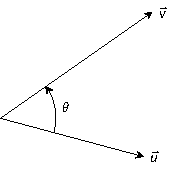
\includegraphics{figures/figdotpangle}\\
(a)\\[15pt]
\myincludegraphicsthree{width=125pt,3Dmenu,activate=onclick,deactivate=onclick,
3Droll=0,
3Dortho=0.0045,
3Dc2c=.54 .61 .58,
3Dcoo=0 0 40,
3Droo=170,
3Dlights=Headlamp,add3Djscript=asylabels.js}{width=125pt}{figures/figdotpangle3D}\\
%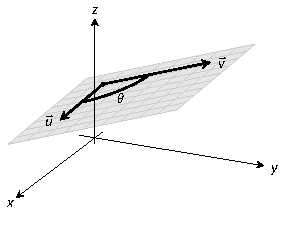
\includegraphics{figures/figdotpangle3D}\\
(b)
\end{tabular}
}

The same is also true of 2 vectors in space: given $\vec u$ and $\vec v$ in $\mathbb{R}^3$ with the same initial point, there is a plane that contains both $\vec u$ and $\vec v$. (When $\vec u$ and $\vec v$ are co-linear, there are infinitely many planes that contain both vectors.) In that plane, we can again find an angle $\theta$ between them (and again, $0\leq \theta\leq \pi$). This is illustrated in Figure \ref{fig:dotpangle}(b).

The following theorem connects this angle $\theta$ to the dot product of $\vec u$ and $\vec v$.

\theorem{thm:dot_product}{The Dot Product and Angles}
{Let $\vec u$ and $\vec v$ be nonzero vectors in $\mathbb{R}^2$ or $\mathbb{R}^3$. Then 
\[
\dotp uv = \norm{\vec u}\,\norm{\vec v} \cos\theta,
\]
where $\theta$, $0\leq\theta\leq \pi$, is the angle between $\vec u$ and $\vec v$.
\index{dot product!properties}\index{vectors!dot product}
}

\mfigure{.16}{Proving Theorem \ref{thm:dot_product}}{fig:dotprodproof}{figures/dotproductproof}

The proof of Theorem \ref{thm:dot_product} is an application of the \href{https://en.wikipedia.org/wiki/Law_of_cosines}{\underline{Law of Cosines}}, using the properties in Theorem \ref{thm:dot_product_properties}. Referring to Figure \ref{fig:dotprodproof}, if we let $a=\norm{\vec u}$, $b=\norm{\vec v}$, and $c = \norm{\vec u-\vec v}$, then the Law of Cosines tells us that
\[
c^2 = a^2+b^2 - 2ab\cos(\theta).
\]
Thus, we have
\begin{align*}
\norm{\vec{u}-\vec{v}}^2 & = \norm{\vec{u}}^2+\norm{\vec{v}}^2-2\norm{\vec{u}}\norm{\vec{v}}\cos\theta\\
(\vec u-\vec v)\cdot(\vec u-\vec v) & = \dotp uu +\dotp vv -2\norm{\vec{u}}\norm{\vec{v}}\cos\theta\\
\dotp uu -\dotp uv - \dotp vu + \dotp vv & = \dotp uu +\dotp vv -2\norm{\vec{u}}\norm{\vec{v}}\cos\theta\\
-2\dotp uv &= -2\norm{\vec{u}}\norm{\vec{v}}\cos\theta\\
\dotp uv &= \norm{\vec{u}}\norm{\vec{v}}\cos\theta,
\end{align*}
as required.

Using Theorem \ref{thm:dot_product_properties}, we can rewrite this theorem as
\[
\frac{\vec u}{\norm{\vec u}}\cdot \frac{\vec v}{\norm{\vec v}} = \cos \theta.
\]
Note how on the left hand side of the equation, we are computing the dot product of two unit vectors. Recalling that unit vectors essentially only provide direction information, we can informally restate Theorem \ref{thm:dot_product} as saying ``The dot product of two directions gives the cosine of the angle between them.''

When $\theta$ is an acute angle (i.e., $0\leq \theta <\pi/2$), $\cos \theta$ is positive; when $\theta = \pi/2$, $\cos \theta = 0$; when $\theta$ is an obtuse angle ($\pi/2<\theta \leq \pi$), $\cos \theta$ is negative. Thus the sign of the dot product gives a general indication of the angle between the vectors, illustrated in Figure \ref{fig:dotpsign}.

\begin{center}
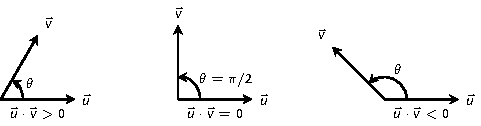
\includegraphics{figures/figdotpanglesign}
\captionsetup{type=figure}
\caption{Illustrating the relationship between the angle between vectors and the sign of their dot product.}
\label{fig:dotpsign}
\end{center}
\vskip\baselineskip

We \emph{can} use Theorem \ref{thm:dot_product} to compute the dot product, but generally this theorem is used to find the angle between known vectors (since the dot product is generally easy to compute). To this end, we rewrite the theorem's equation as
\[
\cos \theta = \frac{\dotp uv}{\norm{\vec u}\norm{\vec v}} \quad \Leftrightarrow \quad \theta = \cos^{-1}\left(\frac{\dotp uv}{\norm{\vec u}\norm{\vec v}}\right).
\]

We practice using this theorem in the following example.\\

\mfigure{.2}{Vectors used in Example \ref{ex_dotp2}.}{fig:dotp2}{figures/figdotp2}
\example{ex_dotp2}{Using the dot product to find angles}{
Let $\vec u = \la 3,1\ra$, $\vec v = \la -2,6\ra$ and $\vec w = \la -4,3\ra$, as shown in Figure \ref{fig:dotp2}. Find the angles $\alpha$, $\beta$ and $\theta$.
}
{We start by computing the magnitude of each vector.
\[
\norm{\vec u} = \sqrt{10};\quad \norm{\vec v} = 2\sqrt{10};\quad \norm{\vec w} = 5.
\]
We now apply Theorem \ref{thm:dot_product} to find the angles.
\begin{align*}
\alpha &= \cos^{-1}\left(\frac{\dotp uv}{(\sqrt{10})(2\sqrt{10})}\right) \\
			&= \cos^{-1}(0) = \frac{\pi}2 = 90^\circ.
\end{align*}
\begin{align*}
\beta &= \cos^{-1}\left(\frac{\dotp vw}{(2\sqrt{10})(5)}\right) \\
			&= \cos^{-1}\left(\frac{26}{10\sqrt{10}}\right) \\
					&\approx 0.6055 \approx 34.7^\circ.\\[10pt]
\theta &= \cos^{-1}\left(\frac{\dotp uw}{(\sqrt{10})(5)}\right) \\
				&= \cos^{-1}\left(\frac{-9}{5\sqrt{10}}\right) \\
				&\approx 2.1763 \approx 124.7^\circ
\end{align*}
\vskip-\baselineskip
}\\

We see from our computation that $\alpha + \beta = \theta$, as indicated by Figure \ref{fig:dotp2}. While we knew this should be the case, it is nice to see that this non-intuitive formula indeed returns the results we expected.
We do a similar example next in the context of vectors in space.\\

%\mfigure{.4}{Vectors used in Example \ref{ex_dotp3}.}{fig:dotp3}{figures/figdotp3}
\example{ex_dotp3}{Using the dot product to find angles}{
Let $\vec u = \la 1,1,1\ra$, $\vec v = \la -1,3,-2\ra$ and $\vec w = \la -5,1,4\ra$, as illustrated in Figure \ref{fig:dotp3}. Find the angle between each pair of vectors.}
{\begin{enumerate}
	\item Between $\vec u$ and $\vec v$:
	\begin{align*}
	\theta &= \cos^{-1}\left(\frac{\dotp uv}{\norm{\vec u}\norm{\vec v}}\right)\\
					&= \cos^{-1}\left(\frac{0}{\sqrt{3}\sqrt{14}}\right)\\
					&= \frac{\pi}2.
	\end{align*}
	\item	Between $\vec u$ and $\vec w$:
	\begin{align*}
	\theta &= \cos^{-1}\left(\frac{\dotp uw}{\norm{\vec u}\norm{\vec w}}\right)\\
					&= \cos^{-1}\left(\frac{0}{\sqrt{3}\sqrt{42}}\right)\\
					&= \frac{\pi}2.
	\end{align*}
	\item	Between $\vec v$ and $\vec w$:
	\begin{align*}
	\theta &= \cos^{-1}\left(\frac{\dotp vw}{\norm{\vec v}\norm{\vec w}}\right)\\
					&= \cos^{-1}\left(\frac{0}{\sqrt{14}\sqrt{42}}\right)\\
					&= \frac{\pi}2.
	\end{align*}
\end{enumerate}
While our work shows that each angle is $\pi/2$, i.e.,  $90^\circ$, none of these angles looks to be a right angle in Figure \ref{fig:dotp3}. Such is the case when drawing three--dimensional objects on the page.
}\\


\mfigurethree{width=150pt,3Dmenu,activate=onclick,deactivate=onclick,
3Droll=0,
3Dortho=0.0045,
3Dc2c=.89 .4 .23,
3Dcoo=10 50 46,
3Droo=200,
3Dlights=Headlamp,add3Djscript=asylabels.js}{width=150pt}{.3}{Vectors used in Example \ref{ex_dotp3}.}{fig:dotp3}{figures/figdotp3}%

All three angles between these vectors was $\pi/2$, or $90^\circ$. We know from geometry and everyday life that $90^\circ$ angles are ``nice'' for a variety of reasons, so it should seem significant that these angles are all $\pi/2$. Notice the common feature in each calculation (and also the calculation of $\alpha$ in Example \ref{ex_dotp2}): the dot products of each pair of angles was 0. We use this as a basis for a definition of the term \textbf{orthogonal}, which is essentially synonymous to \textit{perpendicular}.

\definition{def:orthogonal}{Orthogonal}
{Vectors $\vec u$ and $\vec v$ are \textbf{orthogonal} if their dot product is 0.
\index{orthogonal}\index{perpendicular|see{orthogonal}}\index{vectors!orthogonal}
}

\mnote{.5}{\textbf{Note:} The term \textit{perpendicular} originally referred to lines. As mathematics progressed, the concept of ``being at right angles to'' was applied to other objects, such as vectors and planes, and the term \emph{orthogonal} was introduced. It is especially used when discussing objects that are hard, or impossible, to visualize: two vectors in 5-dimensional space are orthogonal if their dot product is 0. It is not wrong to say they are \textit{perpendicular}, but common convention gives preference to the word \textit{orthogonal}.

Note also that Definition \ref{def:orthogonal} makes sense if either $\vec u$ or $\vec v$ is the zero vector, but this is not the case for the conventional understanding of the word perpendicular.
}

%\pagebreak

\example{ex_dotp8}{Finding orthogonal vectors}{
Let $\vec u = \la 3,5\ra$ and $\vec v = \la 1,2,3\ra$. 
\begin{enumerate}
	\item Find two vectors in $\mathbb{R}^2$ that are orthogonal to $\vec u$.
	\item	Find two non--parallel vectors in $\mathbb{R}^3$ that are orthogonal to $\vec v$.
\end{enumerate}
}
{\begin{enumerate}
	\item Recall that a line perpendicular to a line with slope $m$ has slope $-1/m$, the ``opposite reciprocal slope.'' We can think of the slope of $\vec u$ as $5/3$, its ``rise over run.'' A vector orthogonal to $\vec u$ will have slope $-3/5$. There are many such choices, though all parallel:
	\[
	\la -5,3\ra \quad \text{or} \quad\la 5,-3\ra \quad \text{or} \quad \la -10,6\ra\quad \text{or} \quad \la 15,-9\ra,\text{etc.}
	\]
	\item		There are infinite directions in space orthogonal to any given direction, so there are an infinite number of non--parallel vectors orthogonal to $\vec v$. Since there are so many, we have great leeway in finding some.
	
	One way is to arbitrarily pick values for the first two components, leaving the third unknown. For instance, let $\vec v_1 = \la 2,7,z\ra$. If $\vec v_1$ is to be orthogonal to $\vec v$, then $\vec v_1\cdot\vec v = 0$, so 
	\[
	2+14+3z=0 \quad \Rightarrow z = \frac{-16}{3}.
	\]
	So $\vec v_1 = \la 2, 7, -16/3\ra$ is orthogonal to $\vec v$. We can apply a similar technique by leaving the first or second component unknown.
	
	Another method of finding a vector orthogonal to $\vec v$ mirrors what we did in part 1. Let $\vec v_2 = \la-2,1,0\ra$. Here we switched the first two components of $\vec v$, changing the sign of one of them (similar to the ``opposite reciprocal'' concept before). Letting the third component be 0 effectively ignores the third component of $\vec v$, and it is easy to see that 
	\[
	\vec v_2\cdot\vec v = \la -2,1,0\ra\cdot\la 1,2,3\ra = 0.
	\]
	Clearly $\vec v_1$ and $\vec v_2$ are not parallel.
\end{enumerate}
\vskip-1.5\baselineskip
}\\

An important construction is illustrated in Figure \ref{fig:dotpproj}, where vectors $\vec u$ and $\vec v$ are sketched. In part (a), a dotted line is drawn from the tip of $\vec u$ to the line containing $\vec v$, where the dotted line is orthogonal to $\vec v$. In part (b), the dotted line is replaced with the vector $\vec z$ and  $\vec w$ is formed, parallel to $\vec v$. It is clear by the diagram that $\vec u = \vec w+\vec z$. What is important about this construction is this: $\vec u$ is \emph{decomposed} as the sum of two vectors, one of which is parallel to $\vec v$ and one that is perpendicular to $\vec v$. It is hard to overstate the importance of this construction (as we'll see in upcoming examples). 

The vectors $\vec w$, $\vec z$ and $\vec u$ as shown in Figure \ref{fig:dotpproj} (b) form a right triangle, where the angle between $\vec v$ and $\vec u$ is labelled $\theta$. We can find $\vec w$ in terms of $\vec v$ and $\vec u$.

Using trigonometry, we can state that 
\begin{equation}
\norm{\vec w} = \norm{\vec u}\cos \theta. \label{eq:proj1}
\end{equation}
\mtable{.3}{Developing the construction of the \emph{orthogonal projection}.}{fig:dotpproj}{%
\begin{tabular}{c}
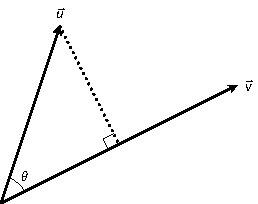
\includegraphics{figures/figdotpproja}\\
(a)\\[15pt]
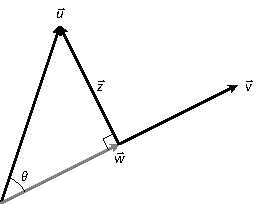
\includegraphics{figures/figdotpprojb}\\
(b)
\end{tabular}
}

We also know that $\vec w$ is parallel to to $\vec v$\,; that is, the direction of $\vec w$ is the direction of $\vec v$, described by the unit vector $\frac{1}{\norm{\vec v}}\vec v$. The vector $\vec w$ is the vector in the direction $\frac{1}{\norm{\vec v}}\vec v$ with magnitude $\norm{\vec u}\cos \theta$:
\begin{align*}
\vec w &= \Big(\norm{\vec u}\cos\theta \Big)\frac{1}{\norm{\vec v}}\vec v.
\intertext{Replace $\cos\theta$ using Theorem \ref{thm:dot_product}:}
			&= \left(\norm{\vec u}\frac{\dotp uv}{\norm{\vec u}\norm{\vec v}}\right)\frac{1}{\norm{\vec v}} \vec v\\ 
			&= \frac{\dotp uv}{\norm{\vec v}^2}\vec v.
			\intertext{Now apply Theorem \ref{thm:dot_product_properties}.}
			&= \frac{\dotp uv}{\dotp vv}\vec v.
\end{align*}

Since this construction is so important, it is given a special name.

\definition{def:orthogonal_projection}{Orthogonal Projection}
{Let nonzero vectors $\vec u$ and $\vec v$ be given. The \textbf{orthogonal projection of $\vec u$ onto $\vec v$}, denoted $\proj uv$, is 
\index{orthogonal projection}\index{vectors!orthogonal projection}
\[
\proj uv = \frac{\dotp uv}{\dotp vv}\vec v.
\]
}

\example{ex_dotp4}{Computing the orthogonal projection}{
\begin{enumerate}
	\item Let $\vec u= \la -2,1\ra$ and $\vec v=\la 3,1\ra$. Find $\proj uv$, and sketch all three vectors with initial points at the origin.
	\item	Let $\vec w = \la 2,1,3\ra$ and $\vec x = \la 1,1,1\ra$. Find $\proj wx$, and sketch all three vectors with initial points at the origin.
\end{enumerate}\pagebreak
}
{\begin{enumerate}
	\item Applying Definition \ref{def:orthogonal_projection}, we have
	\begin{align*}
	\proj uv &= \frac{\dotp uv}{\dotp vv}\vec v \\
					&= \frac{-5}{10}\la 3,1\ra\\
					&= \la -\frac32,-\frac12\ra.
	\end{align*}
	Vectors $\vec u$, $\vec v$ and $\proj uv$ are sketched in Figure \ref{fig:dotp4}(a). Note how the projection is parallel to $\vec v$; that is, it lies on the same line through the origin as $\vec v$, although it points in the opposite direction. That is because the angle between $\vec u$ and $\vec v$ is obtuse (i.e., greater than $90^\circ$).
\mtable{.65}{Graphing the vectors used in Example \ref{ex_dotp4}.}{fig:dotp4}{%
\begin{tabular}{c}
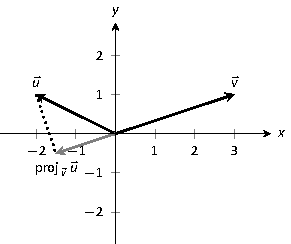
\includegraphics{figures/figdotp4a}\\
(a)\\[15pt]
\myincludegraphicsthree{width=100pt,3Dmenu,activate=onclick,deactivate=onclick,
3Droll=0,
3Dortho=0.0046,
3Dc2c=.9 .12 .42,
3Dcoo=0 50 30,
3Droo=250,
3Dlights=Headlamp,add3Djscript=asylabels.js}{width=100pt}{figures/figdotp4b}\\
%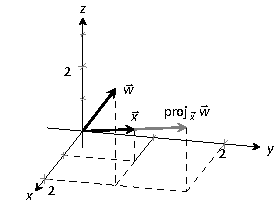
\includegraphics{figures/figdotp4b}\\
(b)\\[15pt]
\myincludegraphicsthree{width=100pt,3Dmenu,activate=onclick,deactivate=onclick,
3Droll=0,
3Dortho=0.0046,
3Dc2c=.29 .77 .56,
3Dcoo=50 0 40,
3Droo=250,
3Dlights=Headlamp,add3Djscript=asylabels.js}{width=100pt}{figures/figdotp4c}\\
%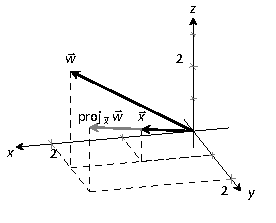
\includegraphics{figures/figdotp4c}\\
(c)\\[15pt]
\end{tabular}
}	
	
	\item		Apply the definition:
	\begin{align*}
	\proj wx &= \frac{\dotp wx}{\dotp xx}\vec x \\
					&= \frac{6}{3}\la 1,1,1\ra\\
					&= \la 2,2,2\ra.
	\end{align*}
	These vectors are sketched in Figure \ref{fig:dotp4}(b), and again in part (c) from a different perspective. Because of the nature of graphing these vectors, the sketch in part (b) makes it difficult  to recognize that the drawn projection has the geometric properties it should. The graph shown in part (c) illustrates these properties better.
\end{enumerate}
\vskip-\baselineskip
}\\

We can use the properties of the dot product found in Theorem \ref{thm:dot_product_properties} to rearrange the formula found in Definition \ref{def:orthogonal_projection}:
\begin{align*}
\proj uv &= \frac{\dotp uv}{\dotp vv}\vec v\\
		&= \frac{\dotp uv}{\norm{\vec v}^2}\vec v\\
		&= \left(\vec u \cdot \frac{\vec v}{\norm{\vec v}}\right) \frac{\vec v}{\norm{\vec v}}.
\end{align*}

The above formula shows that the orthogonal projection of $\vec u$ onto $\vec v$ is only concerned with the \emph{direction} of $\vec v$, as both instances of $\vec v$ in the formula come in the form $\vec v/\norm{\vec v}$, the unit vector in the direction of $\vec v$.

A special case of orthogonal projection occurs when $\vec v$ is a unit vector. In this situation, the formula for the orthogonal projection of a vector $\vec u$ onto $\vec v$ reduces to just $\proj uv = (\vec u\cdot\vec v)\vec v$, as $\vec v\cdot\vec v = 1$.

This gives us a new understanding of the dot product. When $\vec v$ is a unit vector, essentially providing only direction information, the dot product of $\vec u$ and $\vec v$ gives ``how much of $\vec u$ is in the direction of $\vec v$.'' This use of the dot product will be very useful in future sections.\\

\mfigure{.2}{Illustrating the orthogonal projection.}{fig:dotpprojc}{figures/figdotpprojc}
Now consider Figure \ref{fig:dotpprojc} where the concept of the orthogonal projection is again illustrated. It is clear that 
\begin{equation}
\vec u = \proj uv + \vec z.
\label{eq:orthogproj}
\end{equation} As we know what $\vec u$ and $\proj uv$ are, we can solve for $\vec z$ and state that
\[
\vec z = \vec u - \proj uv.
\]
This leads us to rewrite Equation \eqref{eq:orthogproj} in a seemingly silly way: 
\[
\vec u = \proj uv + (\vec u - \proj uv).
\]
This is not nonsense, as pointed out in the following Key Idea. (Notation note: the expression ``$\parallel \vec y$\,'' means ``is parallel to $\vec y$.'' We can use this notation to state ``$\vec x\parallel\vec y$\,'' which means ``$\vec x$ is parallel to $\vec y$.'' The expression ``$\perp \vec y$\,'' means ``is orthogonal to $\vec y$,'' and is used similarly.)

\mnote{.6}{\textbf{Note:} The argument leading to Definition \ref{def:orthogonal_projection} is not quite a proof, since it depended on choices made in forming the diagram in Figure \ref{fig:dotpproj}. However, we can easily verify that the result in Key Idea \ref{idea:orthog_proj} is always valid: since
\begin{align*}
\vec v\cdot(\vec u - \proj uv) & = \dotp vu - \vec v\cdot\left(\frac{\dotp uv}{\norm{\vec{v}}^2}\vec{v}\right)\\
& = \dotp vu -\frac{\dotp uv}{\dotp vv}(\dotp vv)\\
& = \dotp vu - \dotp uv = 0
\end{align*}
for \textbf{any} vectors $\vec u$ and $\vec v\neq \vec 0$, we are guaranteed that the vector $u-\proj uv$ will always be orthogonal to $\vec v$.}

\keyidea{idea:orthog_proj}{Orthogonal Decomposition of Vectors}
{Let nonzero vectors $\vec u$ and $\vec v$ be given. Then $\vec u$ can be written as the sum of two vectors, one of which is parallel to $\vec v$, and one of which is orthogonal to $\vec v$:
\index{orthogonal decomposition of vectors}\index{orthogonal!decomposition}\index{vectors!orthogonal decomposition}
\[
\vec u = \underbrace{\proj uv}_{\parallel\ \vec v}\ +\  (\underbrace{\vec u-\proj uv}_{\perp\ \vec v}).
\]
}

We illustrate the use of this equality in the following example.\\

\example{ex_dotp5}{Orthogonal decomposition of vectors}{
\begin{enumerate}
	\item Let $\vec u = \la -2,1\ra $ and $\vec v = \la 3,1\ra$ as in Example \ref{ex_dotp4}. Decompose $\vec u$ as the sum of a vector parallel to $\vec v$ and a vector orthogonal to $\vec v$.
	\item	Let $\vec w =\la 2,1,3\ra$ and $\vec x  =\la 1,1,1\ra$ as in Example \ref{ex_dotp4}. Decompose $\vec w$ as the sum of a vector parallel to $\vec x$ and a vector orthogonal to $\vec x$.
\end{enumerate}
}
{\begin{enumerate}
	\item In Example \ref{ex_dotp4}, we found that $\proj uv = \la -1.5,-0.5\ra$. Let 
	\[
	\vec z = \vec u - \proj uv = \la -2,1\ra - \la -1.5,-0.5\ra = \la-0.5, 1.5\ra.
	\]
	Is $\vec z$ orthogonal to $\vec v$\,? (I.e, is $\vec z \perp\vec v$\ ?) We check for orthogonality with the dot product:
	\[
	\dotp zv = \la -0.5,1.5\ra \cdot \la 3,1\ra =0.
	\]
	Since the dot product is 0, we know $\vec z \perp \vec v$. Thus:
	\begin{align*}
	\vec u &= \proj uv\ +\ (\vec u - \proj uv) \\
	\la -2,1\ra &= \underbrace{\la -1.5,-0.5\ra}_{\parallel\ \vec v}\ +\ \underbrace{\la -0.5,1.5\ra}_{\perp \ \vec v}.
	\end{align*}
	
	\item	We found in Example \ref{ex_dotp4} that $\proj wx = \la 2,2,2\ra$. Applying the Key Idea, we have:
	\[
	\vec z = \vec w - \proj wx = \la 2,1,3\ra  - \la 2,2,2\ra = \la 0,-1,1\ra.
	\]
	We check to see if $\vec z \perp \vec x$:
	\[
	\dotp zx = \la 0,-1,1\ra \cdot \la 1,1,1\ra = 0.
	\]
	Since the dot product is 0, we know the two vectors are orthogonal.
	We now write $\vec w$ as the sum of two vectors, one parallel and one orthogonal to $\vec x$:
	\begin{align*}
	\vec w &= \proj wx\ +\ (\vec w - \proj wx) \\
	\la 2,1,3\ra &= \underbrace{\la 2,2,2\ra}_{\parallel\ \vec x}\ +\ \underbrace{\la 0,-1,1\ra}_{\perp \ \vec x} 
	\end{align*}
\end{enumerate}
\vskip-\baselineskip
}\\

We give an example of where this decomposition is useful.\\

\example{ex_dotp6}{Orthogonally decomposing a force vector}{
Consider Figure \ref{fig:dotp6}(a), showing a box weighing 50 lb on a ramp that rises 5 ft over a span of 20 ft. Find the components of force, and their magnitudes, acting on the box (as sketched in part (b) of the figure):
\mtable{.4}{Sketching the ramp and box in Example \ref{ex_dotp6}. Note: \textit{The vectors are not drawn to scale.}}{fig:dotp6}{%
\begin{tabular}{c}
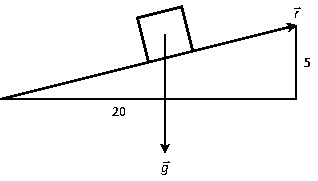
\includegraphics{figures/figdotp6}\\
(a)\\[15pt]
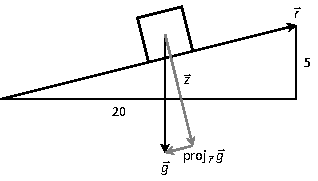
\includegraphics{figures/figdotp6b}\\
(b)
\end{tabular}
}
\begin{enumerate}
	\item in the direction of the ramp, and
	\item	orthogonal to the ramp.
\end{enumerate}
}
{As the ramp rises 5 ft over a horizontal distance of 20 ft, we can represent the direction of the ramp with the vector $\vec r= \la 20,5\ra$. Gravity pulls down with a force of 50 lb, which we represent with $\vec g = \la 0,-50\ra$. 
\begin{enumerate}
	\item To find the force of gravity in the direction of the ramp, we compute $\proj gr$:
	\begin{align*}
	\proj gr &= \frac{\dotp gr}{\dotp rr}\vec r\\
					&=  \frac{-250}{425}\la 20,5\ra\\
					&= \la -\frac{200}{17},-\frac{50}{17}\ra \approx \la -11.76,-2.94\ra.
	\end{align*}
	The magnitude of $\proj gr$ is $\norm{\proj gr} = 50/\sqrt{17} \approx 12.13\text{ lb}$. Though the box weighs 50 lb, a force of about 12 lb is enough to keep the box from sliding down the ramp.
	
	\item		To find the component $\vec z$ of gravity orthogonal to the ramp, we use Key Idea \ref{idea:orthog_proj}.
	\begin{align*}
	\vec z &= \vec g - \proj gr \\
					&= \la \frac{200}{17},-\frac{800}{17}\ra \approx \la 11.76,-47.06\ra.
	\end{align*}
	The magnitude of this force is $\norm{\vec z} \approx 48.51$ lb. In physics and engineering, knowing this force is important when computing things like static frictional force. (For instance, we could easily compute if the static frictional force alone was enough to keep the box from sliding down the ramp.)
\end{enumerate}
\vskip-\baselineskip
}\pagebreak

\noindent\textbf{\large Application to Work}\\

In physics, the application of a force $F$ to move an object in a straight line a distance $d$ produces \emph{work}; the amount of work $W$ is $W=Fd$, (where $F$ is in the direction of travel). The orthogonal projection allows us to compute work when the force is not in the direction of travel.

Consider Figure \ref{fig:dotpwork}, where a force $\vec F$ is being applied to an object moving in the direction of $\vec d$. (The distance the object travels is the magnitude of $\vec d$.) The work done is the amount of force in the direction of $\vec d$, $\norm{\proj Fd}$, times $\vnorm d$:
\mfigure{.75}{Finding work when the force and direction of travel are given as vectors.}{fig:dotpwork}{figures/figdotpwork}

\begin{align*}
\norm{\proj Fd}\cdot\vnorm d &= \snorm{\frac{\dotp Fd}{\dotp dd}\vec d}\cdot \vnorm d \\
		&= \left\lvert\frac{\dotp Fd}{\vnorm d^2}\right\rvert\cdot \vnorm d\cdot\vnorm d\\
		&= \frac{\left\lvert\dotp Fd\right\rvert}{\vnorm d^2}\vnorm d^2\\
		&= \left\lvert\dotp Fd\right\rvert.
\end{align*}

The expression $\dotp Fd$ will be positive if the angle between $\vec F$ and $\vec d$ is acute; when the angle is obtuse (hence $\dotp Fd$ is negative), the force is causing motion in the opposite direction of $\vec d$, resulting in ``negative work.'' We want to capture this sign, so we drop the absolute value and find that $W = \dotp Fd$.

\definition{def:work}{Work}
{Let $\vec F$ be a constant force that moves an object in a straight line from point $P$ to point $Q$. Let $\vec d = \vv{PQ}$. The \textbf{work} $W$ done by $\vec F$ along $\vec d$ is $W = \dotp Fd$.
\index{work}
}

\example{ex_dotp7}{Computing work}{
A man slides a box along a ramp that rises 3 ft over a distance of 15 ft by applying 50 lb of force as shown in Figure \ref{fig:dotp7}. Compute the work done.}
{The figure indicates that the force applied makes a $30^\circ$ angle with the horizontal, so $\vec F = 50\la \cos 30^\circ,\sin 30^\circ\ra \approx \la 43.3,25\ra.$ The ramp is represented by $\vec d  = \la 15,3\ra$. The work done is simply
\[
\dotp Fd = 50\la \cos 30^\circ,\sin 30^\circ\ra \cdot \la 15,3\ra \approx 724.5 \text{ ft--lb}.
\]

\mfigure{.35}{Computing work when sliding a box up a ramp in Example \ref{ex_dotp7}.}{fig:dotp7}{figures/figdotp7}
Note how we did not actually compute the distance the object travelled, nor the magnitude of the force in the direction of travel; this is all inherently computed by the dot product!
}\\

The dot product is a powerful way of evaluating computations that depend on angles without actually using angles. The next section explores another ``product'' on vectors, the \emph{cross product.} Once again, angles play an important role, though in a much different way.

\printexercises{exercises/10_03_exercises}

\section{The Cross Product}\label{sec:cross_product}

``Orthogonality'' is immensely important. A quick scan of your current environment will undoubtedly reveal numerous surfaces and edges that are perpendicular to each other (including the edges of this page). The dot product provides a quick test for orthogonality:  vectors $\vec u$ and $\vec v$ are perpendicular if, and only if, $\dotp uv=0$. 

Given two non--parallel, nonzero vectors $\vec u$ and $\vec v$ in space, it is very useful to find a vector $\vec w$ that is perpendicular to both $\vec u$ and $\vec v$. There is a operation, called the \textbf{cross product}, that creates such a vector. This section defines the cross product, then explores its properties and applications.

\definition{def:cross_product}{Cross Product}
{Let $\vec u =\la u_1,u_2,u_3\ra$ and $\vec v = \la v_1,v_2,v_3\ra$ be vectors in $\mathbb{R}^3$. The \textbf{cross product of $\vec u$ and $\vec v$}, denoted $\crossp uv$, is the vector
\index{vectors!cross product}\index{cross product!definition}
\[
\crossp uv = \la u_2v_3-u_3v_2,-(u_1v_3-u_3v_1),u_1v_2-u_2v_1\ra.
\]
}

\mnote{.6}{The definition of the cross product may look strange (and complicated) at first, but it's more or less forced by the requirement that it be orthogonal to both $\vec u$ and $\vec v$. To begin to see why, suppose $\vec w = \la a,b,c\ra$ is an arbitrary vector such that $\dotp wu=0$ and $\dotp wv=0$. This gives us the pair of equations
\begin{align*}
u_1a+u_2b+u_3c&=0\\
v_1a+v_2b+v_3c&=0.
\end{align*}
This is a \textit{system of linear equations} in the variables $a$, $b$, and $c$. Using Gaussian elimination (recalling your linear algebra), it's easy to show that (up to a scalar multiple) the solution is given by Definition \ref{def:cross_product}.}

This definition can be a bit cumbersome to remember. After an example we will give a convenient method for computing the cross product. For now, careful examination of the products and differences given in the definition should reveal a pattern that is not too difficult to remember. (For instance, in the first component only 2 and 3 appear as subscripts; in the second component, only 1 and 3 appear as subscripts. Further study reveals the order in which they appear.)

Let's practice using this definition by computing a cross product.\\

\example{ex_crossp1}{Computing a cross product}{
Let $\vec u = \la 2,-1,4\ra$ and $\vec v = \la 3,2,5\ra$. Find $\crossp uv$, and verify that it is orthogonal to both $\vec u$ and $\vec v$.
}
{Using Definition \ref{def:cross_product}, we have
\begin{align*}
\crossp uv &= \la u_2v_3-u_3v_2,u_3v_1-u_1v_3,u_1v_2-u_2v_1\ra\\
		   &= \la (-1)5-(4)2,(4)3-(2)5, (2)2-(-1)3\ra = \la -13,2,7\ra.
\end{align*}
(We encourage the reader to compute this product on their own, then verify their result.)

\enlargethispage{2\baselineskip}
We test whether or not $\crossp uv$ is orthogonal to $\vec u$ and $\vec v$ using the dot product:
\begin{align*}
\big(\crossp uv\big) \cdot \vec u &= \la -13,2,7\ra \cdot \la 2,-1,4\ra = 0,\\
\big(\crossp uv\big) \cdot \vec v &= \la -13,2,7\ra \cdot \la 3,2,5 \ra = 0.
\end{align*}
Since both dot products are zero, $\crossp uv$ is indeed orthogonal to both $\vec u$ and $\vec v$.
}\\

We now introduce a method for computing the cross-product that is easier to remember, which you may recall from your first course in linear algebra.

Consider a matrix $\begin{bmatrix} a&b\\c&d\end{bmatrix}$ of four real numbers $a,b,c$, and $d$. A $2\times 2$ determinant takes any such matrix and assigns the number $ad-bc$. This is commonly denoted as follows:
\[
\begin{vmatrix} a&b\\c&d\end{vmatrix} = ad-bc.
\]
Most people find it easiest to remember this in terms of the two \textit{diagonals} of the array: we take the product of the two numbers on the \textit{main diagonal} (top-left to bottom-right), and subtract the product of the two numbers on the other diagonal:
\btz [baseline=-3pt,>=stealth]
\node at (0,0) {$\begin{vmatrix} a & b\\ c& d\end{vmatrix}$};
\draw[->,  thin] (-.5,.4) -- (.6,-.6) node[below right] {$ad\vphantom{bc}$};
\draw[->, thin] (0.4,.4) -- (-.6,-.6) node[below left ] {$bc$};
\etz

For example, we have $\begin{vmatrix} 4&-2\\6&3\end{vmatrix} = 4(3)-(-2)(6)=24$. Once we get comfortable with $2\times 2$ determinants, we can write the cross product in terms of them, as follows:
\begin{align}
\crossp uv &= \begin{vmatrix} u_2&u_3\\v_2&v_3\end{vmatrix} \veci - \begin{vmatrix} u_1&u_3\\v_1&v_3\end{vmatrix}\vecj + \begin{vmatrix} u_1&u_2\\v_1&v_2\end{vmatrix}\veck\label{eq:crossdet}\\ 
& = (u_2v_3-u_3v_2)\veci-(u_3v_1-u_1v_3)\vecj + (u_1v_2-u_2v_1)\veck,\nonumber
\end{align}
as before. Now, this might not seem like much of an improvement over the previous formula, so we take things one step further. First, we form a $3\times 3$ array as shown below. 
\[
\begin{vmatrix} \veci&\vecj&\veck\\u_1&u_2&u_3\\v_1&v_2&v_3\end{vmatrix}.
\]
The first row comprises the standard unit vectors $\vec i$, $\vec j$, and $\vec k$. The second and third rows are the vectors $\vec u$ and $\vec v$, respectively. Next, we \textit{expand} our $3\times 3$ array as a vector, where the coefficient of each standard unit vector is given by the $2\times 2$ determinant that's left over when we delete the row and column containing that unit vector. 

For example, if we use $\vec u$ and $\vec v$ from Example \ref{ex_crossp1}, we obtain the array
\[
\begin{vmatrix} \veci&\vecj&\veck \\  2&-1&4\\3&2&5\end{vmatrix}.
\]
The expansion process used to obtain the coefficients of $\veci, \vecj \veck$ looks like the following:

\btz [baseline=-3pt,>=stealth]
\node at (0,0) {$\begin{vmatrix} \fbox{\veci}&\vecj&\veck \\  2&-1&4\\3&2&5\end{vmatrix}\longrightarrow \begin{vmatrix} -1&4\\2&5\end{vmatrix}\veci = -13\veci$};
\draw[thin] (-2.3,.6) -- (-2.3, -.6);
\draw[thin] (-2.5,.4) -- (-.8,.4);
\etz

Now repeat the first two columns after the original three:
\btz [baseline=-3pt,>=stealth]
\node at (0,0) {$\begin{vmatrix} \veci&\fbox{\vecj}&\veck \\  2&-1&4\\3&2&5\end{vmatrix}\longrightarrow \begin{vmatrix} 2&4\\3&5\end{vmatrix}\vecj = -2\vecj$};
\draw[thin] (-1.45,.6) -- (-1.45, -.6);
\draw[thin] (-2.3,.4) -- (-.6,.4);
\etz

This gives three full ``upper left to lower right'' diagonals, and three full ``upper right to lower left'' diagonals, as shown. Compute the products along each diagonal, then add the products on the right and subtract the products on the left:

\btz [baseline=-3pt,>=stealth]
\node at (0,0) {$\begin{vmatrix} \veci&\vecj&\fbox{\veck} \\  2&-1&4\\3&2&5\end{vmatrix}\longrightarrow \begin{vmatrix} 2&-1\\3&2\end{vmatrix}\veck = 7\veck$};
\draw[thin] (-0.85,.6) -- (-0.85, -.6);
\draw[thin] (-2.3,.4) -- (-.6,.4);
\etz
\[
\crossp uv = \big(-5\veci+12\vecj+4\veck\,\big) - \big(-3\veck+8\veci+10\vecj\,\big) = -13\veci+2\vecj+7\veck = \la -13,2,7\ra.
\]

There is one more important detail to note: notice in Equation \eqref{eq:crossdet} that there is a \textbf{minus sign} in front of the coefficient of the unit vector $\vecj$. We need to make sure that the signs in front of each $2\times 2$ determinant follow this $+,\,-,\,+$ pattern when we expand our array as a vector. For the vectors $\vec u$ and $\vec v$ in Example \ref{ex_crossp1}, we end up with the following:
\begin{align*}
\crossp uv & = \begin{vmatrix} \veci&\vecj&\veck \\  2&-1&4\\3&2&5\end{vmatrix}  = \begin{vmatrix} -1&4\\2&5\end{vmatrix}\veci - \begin{vmatrix} 2&4\\3&5\end{vmatrix}\vecj + \begin{vmatrix} 2&-1\\3&2\end{vmatrix}\veck\\
& = -13\veci - (-2)\vecj + 7\veck = \la -13, 2, 7\ra,
\end{align*}
as before. The method will become more clear with a bit of practice.\\

\mnote{.75}{\textbf{Note:} If the minus sign in front of the $\vecj$ coefficient seems out of place to you, it might help to imagine wrapping our $3\times 3$ array around a cylinder (like the label on a tin can). If we read from left to right, \textit{beginning in the $\vecj$ column}, then we should place the $\veck$ column first, followed by the $\veci$ column. For the vectors $\vec{u}$ and $\vec{v}$ in Example \ref{ex_crossp1}, this would result in the coefficient $\begin{vmatrix} 4&2\\5&2\end{vmatrix} = 2$ for the $\vecj$ component, which has the correct sign. However, since our habit is to read starting from the far left, we tend to write the $\veci$ column first, and then introduce the minus sign to compensate.}


\example{ex_crossp2}{Computing a cross product}{
Let $\vecu=\la 1,3,6\ra$ and $\vec v = \la -1,2,1\ra$. Compute both $\crossp uv$ and $\crossp vu$.}
{To compute $\crossp uv$, we form our $3\times 3$ array as prescribed above, and expand it into a vector:
\begin{align*}
\crossp uv &= \begin{vmatrix} \veci & \vecj & \veck\\ 1& 3& 6\\ -1& 2& 1\end{vmatrix} = \begin{vmatrix} 3& 6\\2 &1\end{vmatrix} \veci - \begin{vmatrix} 1 & 6\\ -1& 1\end{vmatrix}\vecj +\begin{vmatrix} 1& 3\\ -1 & 2\end{vmatrix}\veck\\
		& = (3(1)-6(2))\veci -(1(1)-6(-1))\vecj + (1(2)-3(-1))\veck\\
		& = -9\veci-7\vecj+5\veck = \la -9, -7, 5\ra.
\end{align*}
To compute $\crossp vu$, we switch the second and third rows of the above matrix, then expand as before:
\begin{align*}
\crossp vu & = \begin{vmatrix} \veci & \vecj& \veck\\ -1 & 2& 1\\ 1& 3& 6\end{vmatrix} = \begin{vmatrix} 2 &1\\3 &6\end{vmatrix}\veci - \begin{vmatrix} -1& 1\\ 1& 6\end{vmatrix}\vecj + \begin{vmatrix} -1& 2\\ 1 &3\end{vmatrix}\veck\\
		   & = (2(6)-1(3))\veci-((-1)(6)-1(1))\vecj + ((-1)(3)-2(1))\veck\\
		   & = 9\veci+7\vecj -5\veck = \la 9, 7, -5\ra = -\crossp uv.
\end{align*}
Note how with the rows being switched, the products that once appeared on the right now appear on the left, and vice--versa, so that the result is the opposite of $\crossp uv$. We leave it to the reader to verify that each of these vectors is orthogonal to $\vec u$ and $\vec v$.
}\\

\noindent\textbf{\large Properties of the Cross Product}\\

It is not coincidence that $\crossp vu = -(\crossp uv)$ in the preceding example; one can show using Definition \ref{def:cross_product} that this will always be the case. The following theorem states several useful properties of the cross product, each of which can be verified by referring to the definition.

\setboxwidth{15pt}
%\noindent\hskip-50pt\begin{minipage}{\linewidth}
\theorem{thm:cross_prod_prop}{Properties of the Cross Product}
{Let $\vecu$, $\vecv$ and $\vecw$ be vectors in $\mathbb{R}^3$ and let $c$ be a scalar. The following identities hold:
\index{vectors!cross product}\index{cross product!properties}
\begin{enumerate}
	\item \parbox{167pt}{$\crossp uv = -(\crossp vu)$} Anticommutative Property
	\item	\begin{enumerate}
		\item \parbox{145pt}{$(\vec u+\vec v)\times \vecw = \crossp uw+\crossp vw$} Distributive Properties
		\item	$\vec u \times (\vec v+\vec w) = \crossp uv+\crossp uw$
	\end{enumerate}
	\item		$c(\crossp uv) = (c\vecu) \times \vec v = \vecu \times (c\vecv)$
	\item		\begin{enumerate}
		\item \parbox{145pt}{$(\crossp uv)\cdot \vecu = 0$} Orthogonality Properties
		\item	$(\crossp uv)\cdot \vecv = 0$
	\end{enumerate}
	\item		$\crossp uu = \vec 0$
	\item		$\crossp u0 = \vec 0$
	\item		\parbox{167pt}{$\vecu \cdot (\vecv\times\vecw) = (\crossp uv)\cdot \vecw$} Triple Scalar Product
\end{enumerate}
}
%\end{minipage}
\restoreboxwidth

We introduced the cross product as a way to find a vector orthogonal to two given vectors, but we did not give a proof that the construction given in Definition \ref{def:cross_product} satisfies this property. Theorem \ref{thm:cross_prod_prop} asserts this property holds; we leave it as a problem in the Exercise section to verify this.

The algebraic properties of the cross product in Theorem \ref{thm:cross_prod_prop} also give us an additional method for computing the cross product in terms of the unit vectors $\veci, \vecj, \veck$. We know from Property 5 that
\[
\veci\times\veci = \vec 0, \vecj\times\vecj = \vec 0, \veck\times\veck = \vec 0,
\]
and it's easy to check that
\[
\veci\times\vecj = \veck, \vecj\times\veck = \veci, \veck\times\veci=\vecj,
\]
and then Property 1 guarantees that
\[
\vecj\times \veci = -\veck, \veck\times\vecj = -\veci, \veci\times\veck = -\vecj.
\]
Using Properties 2 and 3, we can then compute, for example,
\begin{align*}
\la 2,0,3\ra\times \la -1,4,2\ra & = (2\veci +3\veck)\times (-\veci +4\vecj +2\veck)\\
& = -2(\veci \times \veci)+8(\veci \times\vecj)+4(\veci \times\veck)\\
& \quad \quad-3(\veck\times\veci)+12(\veck\times\vecj)+6(\veck\times\veck)\\
& = \vec 0+8\veck -4\vecj -3\vecj -12\veci + \vec 0 = \la -12, -7, 8\ra.
\end{align*}

Property 5 from the theorem is also left to the reader to prove in the Exercise section, but it reveals something more interesting than ``the cross product of a vector with itself is $\vec 0$.'' Let $\vec u$ and $\vec v$ be parallel vectors; that is, let there be a scalar $c$ such that $\vecv = c\vecu$. Consider their cross product:
\begin{align*}
\crossp uv &= \vecu \times (c\vec u) \\
					&=	\parbox{50pt}{$c(\crossp uu)$}\text{(by Property 3 of Theorem \ref{thm:cross_prod_prop})}\\
					&= \parbox{50pt}{$\vec 0$.}\text{(by Property 5 of Theorem \ref{thm:cross_prod_prop})}
\end{align*}

We have just shown that the cross product of parallel vectors is $\vec 0$. This hints at something deeper. Theorem \ref{thm:dot_product} related the angle between two vectors and their dot product; there is a similar relationship relating the cross product of two vectors and the angle between them, given by the following theorem.

\theorem{thm:cross_product}{The Cross Product and Angles}
{Let $\vec u$ and $\vec v$ be vectors in $\mathbb{R}^3$. Then
\[
\norm{\crossp uv} = \vnorm u\, \vnorm v \sin\theta,
\]
where $\theta$, $0\leq \theta \leq \pi$, is the angle between $\vecu$ and $\vecv$.
\index{vectors!cross product}\index{cross product!properties}
}

\mnote{.52}{\textbf{Note:} We could rewrite Definition \ref{def:orthogonal} and Theorem \ref{thm:cross_product} to include $\vec 0$, then define that $\vec u$ and $\vec v$ are parallel if $\vec u\times\vec v=\vec 0$. Since $\vec 0\cdot \vec v =0$ and $\vec 0\times \vec v = \vec 0$, this would mean that $\vec 0$ is both parallel \emph{and} orthogonal to all vectors.
%Definition \ref{def:orthogonal} (through Theorem \ref{thm:dot_product}) defines $\vec u$ and $\vec v$ to be orthogonal if $\vec u\cdot\vec v=\vec 0$. We could rewrite Theorem \ref{thm:cross_product} to include $\vec 0$, then define that $\vec u$ and $\vec v$ are parallel if $\vec u\times \vec v =\vec 0$. By such a definition, $\vec 0$ would be both orthogonal and parallel to every vector. 
Apparent paradoxes such as this are not uncommon in mathematics and can be very useful. (See also the marginal note on page \pageref{note:parallel}.)\label{note:crossp}}
Note that this theorem makes a statement about the \emph{magnitude} of the cross product. When the angle between $\vecu$ and $\vecv$ is 0 or $\pi$ (i.e., the vectors are parallel), the magnitude of the cross product is 0. The only vector with a magnitude of 0 is $\vec 0$ (see Property \ref{thm:zero_norm} of Theorem \ref{thm:vector_properties}), hence the cross product of  parallel vectors is $\vec 0$.

We provide some anecdotal evidence of the truth of this theorem in the following example.\\

\example{ex_crossp3}{The cross product and angles}{
Let $\vec u = \la 1,3,6\ra$ and $\vec v = \la -1,2,1\ra$ as in Example \ref{ex_crossp2}. Verify Theorem \ref{thm:cross_product} by finding $\theta$, the angle between $\vecu$ and $\vecv$, and the magnitude of $\crossp uv$.}
{We use Theorem \ref{thm:dot_product} to find the angle between $\vecu$ and $\vecv$. 
\begin{align*}
\theta &= \cos^{-1}\left(\frac{\dotp uv}{\vnorm u\, \vnorm v}\right) \\
			&= \cos^{-1}\left(\frac{11}{\sqrt{46}\sqrt{6}}\right)\\
			&\approx 0.8471 = 48.54^\circ.
\end{align*}

Our work in Example \ref{ex_crossp2} showed that $\crossp uv = \la -9,-7,5\ra$, hence $\norm{\crossp uv} = \sqrt{155}.$ Is $\norm{\crossp uv} = \vnorm u\, \vnorm v\sin\theta$? Using numerical approximations, we find:
\begin{align*}
\norm{\crossp uv} &=\sqrt{155}  & \vnorm u\,\vnorm v \sin\theta & = \sqrt{46}\sqrt{6}\sin 0.8471\\
									&\approx 12.45. & &\approx 12.45.
\end{align*}
Numerically, they seem equal. Using a right triangle, one can show that 
\[
\sin\left(\cos^{-1}\left(\frac{11}{\sqrt{46}\sqrt{6}}\right)\right) = \frac{\sqrt{155}}{\sqrt{46}\sqrt{6}},
\]
which allows us to verify the theorem exactly.
}\\

To see that Theorem \ref{thm:cross_product} holds in general, let $\vec u=\la u_1,u_2,u_3\ra$ and $\vec v =\la v_1,v_2,v_3\ra$ be two arbitrary three-dimensional vectors. Since the angle between $\vec u$ and $\vec v$ is defined to lie between 0 and $\pi$, we know that $\sin\theta\geq 0$, so that both sides of the equation $\norm{\crossp uv} = \norm{\vec{u}}\norm{\vec v}\sin\theta$ are positive. Thus, we can show that both sides are equal if we can show that their squares are equal. We have
\begin{align*}
(\norm{\vec u}\norm{\vec v}\sin\theta)^2 & = \norm{\vec u}^2\norm{\vec v}^2\sin^2\theta\\
& = \norm{\vec u}^2\norm{\vec v}^2(1-\cos^2\theta) \tag*{since $\sin^2\theta+\cos^2\theta=1$}\\
& = \norm{\vec u}^2\norm{\vec v}^2-(\norm{\vec u}\norm{\vec v}\cos\theta)^2\\
& = \norm{\vec u}^2\norm{\vec v}^2-(\dotp uv)^2 \tag*{by Theorem \ref{thm:dot_product}}\\
& = (u_1^2+u_2^2+u_3^2)(v_1^2+v_2^2+v_3^2)-(u_1v_1+u_2v_2+u_3v_3)^2\\
& = u_2^2v_3^2 - 2u_2u_3v_2v_3 + u_3^2v_2^2 + u_1v_3^2 - 2u_1u_3v_1v_3 \tag*{$+ u_3^2v_1^2 + u_1^2v_2^2 - 2u_1u_2v_1v_2 + u_2^2v_1^2$}\\
& = (u_2v_3-u_3v_2)^2+(u_3v_1-u_1v_3)^2+(u_1v_2-u_2v_2)^2\\
& = \norm{\crossp uv}^2,
\end{align*}
as required.\\




\noindent\textbf{Right Hand Rule}\\

The anticommutative property of the cross product demonstrates that $\crossp uv$ and $\crossp vu$ differ only by a sign -- these vectors have the same magnitude but point in the opposite direction. When seeking a vector perpendicular to $\vec u$ and $\vec v$, we essentially have two directions to choose from, one in the direction of $\crossp uv$ and one in the direction of $\crossp vu$. Does it matter which we choose? How can we tell which one we will get without graphing, etc.?

Another wonderful property of the cross product, as defined, is that it follows the \textbf{right hand rule.} Given $\vec u$ and $\vec v$ in $\mathbb{R}^3$ with the same initial point, point the index finger of your right hand in the direction of $\vecu$ and let your middle finger point in the direction of $\vecv$ (much as we did when establishing the right hand rule for the 3-dimensional coordinate system). Your thumb will naturally extend in the direction of $\crossp uv$. One can ``practice'' this using Figure \ref{fig:crossp_rhr}. If you switch, and point the index finder in the direction of $\vecv$ and the middle finger in the direction of $\vecu$, your thumb will now point in the opposite direction, allowing you to ``visualize'' the anticommutative property of the cross product.\index{right hand rule!of the cross product}
\mfigurethree{width=150pt,3Dmenu,activate=onclick,deactivate=onclick,
3Droll=0,
3Dortho=0.0044,
3Dc2c=.78 .32 .53,
3Dcoo=0 0 34,
3Droo=150,
3Dlights=Headlamp,add3Djscript=asylabels.js}{width=150pt}{.55}{Illustrating the Right Hand Rule of the cross product.}{fig:crossp_rhr}{figures/figcrossp_rhr}
%\mfigure[scale=1.25,trim=5mm 5mm 5mm 5mm,clip=true]{.5}{Illustrating the Right Hand Rule of the cross product.}{fig:crossp_rhr}{figures/figcrossp_rhr}

\vskip\baselineskip
\noindent\textbf{\large Applications of the Cross Product}\\

There are a number of ways in which the cross product is useful in mathematics, physics and other areas of science beyond ``just'' finding a vector perpendicular to two others. We highlight a few here.\index{cross product!applications}\\
%\enlargethispage{\baselineskip}
%\clearpage\enlargethispage{2\baselineskip}

\noindent\textbf{Area of a Parallelogram}\\

It is a standard geometry fact that the area of a parallelogram is $A = bh$, where $b$ is the length of the base and $h$ is the height of the parallelogram, as illustrated in Figure \ref{fig:crossp_parallelogram}(a). As shown when defining the Parallelogram Law of vector addition, two vectors $\vecu$ and $\vecv$ define a parallelogram when drawn from the same initial point, as illustrated in Figure \ref{fig:crossp_parallelogram}(b). Trigonometry tells us that $h = \vnorm u \sin \theta$, hence the area of the parallelogram is 
\begin{equation}A = \vnorm u\,\vnorm v\sin\theta = \norm{\crossp uv},\label{eq:crossp1}\end{equation}
where the second equality comes from Theorem \ref{thm:cross_product}.
\mtable{.25}{Using the cross product to find the area of a parallelogram.}{fig:crossp_parallelogram}{%
\begin{tabular}{c}
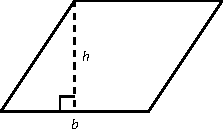
\includegraphics{figures/figcrossp_parallelogram1}\\
(a) \\[15pt]
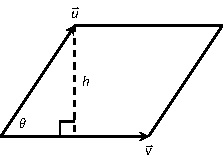
\includegraphics{figures/figcrossp_parallelogram2}\\
(b) \\
\end{tabular}
}
We illustrate using Equation \eqref{eq:crossp1} in the following example.
\index{cross product!applications!area of parallelogram}\\

\example{ex_crossp4}{Finding the area of a parallelogram}{
\begin{enumerate}
	\item Find the area of the parallelogram defined by the vectors $\vecu = \la 2,1\ra$ and $\vecv = \la 1,3\ra$.
	\item	Verify that the points $A = (1,1,1)$, $B = (2,3,2)$, $C = (4,5,3)$ and $D = (3,3,2)$ are the vertices of a parallelogram. Find the area of the parallelogram.
\end{enumerate}
}
{\begin{enumerate}
	\item Figure \ref{fig:crossp4}(a) sketches the parallelogram defined by the vectors $\vec u$ and $\vec v$. We have a slight problem in that our vectors exist in $\mathbb{R}^2$, not $\mathbb{R}^3$, and the cross product is only defined on vectors in $\mathbb{R}^3$. We skirt this issue by viewing $\vec u$ and $\vecv$ as vectors in the $x-y$ plane of $\mathbb{R}^3$, and rewrite them as $\vec u = \la 2,1,0\ra$ and $\vecv =\la 1,3,0\ra$. We can now compute the cross product. 
	It is easy to show that $\crossp uv = \la 0,0,5\ra$; therefore the area of the parallelogram is $A = \norm{\crossp uv} = 5$.
	\mtable{.7}{Sketching the parallelograms in Example \ref{ex_crossp4}.}{fig:crossp4}{%
	\begin{tabular}{c}
	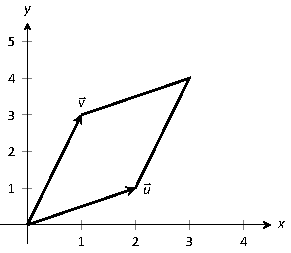
\includegraphics{figures/figcrossp4b}\\
	(a)\\[15pt]
	\myincludegraphicsthree{width=125pt,3Dmenu,activate=onclick,deactivate=onclick,
3Droll=0,
3Dortho=0.004,
3Dc2c=.42 .87 .26,
3Dcoo=61 60 63,
3Droo=250,
3Dlights=Headlamp,add3Djscript=asylabels.js}{width=125pt}{figures/figcrossp4a}\\
	%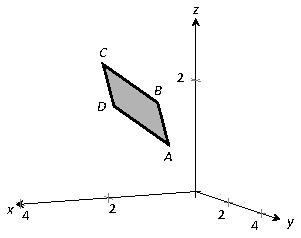
\includegraphics{figures/figcrossp4a}\\
	(b)
	\end{tabular}
	}
	\item		To show that the quadrilateral $ABCD$ is a parallelogram (shown in Figure \ref{fig:crossp4}(b)), we need to show that the opposite sides are parallel. We can quickly show that $\vv{AB} =\vv{DC} = \la 1,2,1\ra$ and $\vv{BC} = \vv{AD} = \la 2,2,1\ra$. We find the area by computing the magnitude of the cross product of $\vv{AB}$ and $\vv{BC}$:
	\[
	\vv{AB} \times \vv{BC} = \la 0,1,-2\ra \quad \Rightarrow \quad \norm{\vv{AB}\times\vv{BC}} = \sqrt{5} \approx 2.236.
	\]
\end{enumerate}
\vskip-\baselineskip
}\\

This application is perhaps more useful in finding the area of a triangle (in short, triangles are used more often than parallelograms). We illustrate this in the following example.\\

\example{ex_crossp5}{Area of a triangle}{
Find the area of the triangle with vertices $A=(1,2)$, $B=(2,3)$ and $C=(3,1)$, as pictured in Figure \ref{fig:crossp5}.}
{We found the area of this triangle in Example \ref{II-ex_abc4} to be $1.5$ using integration. There we discussed the fact that finding the area of a triangle can be inconvenient using the ``$\frac12bh$'' formula as one has to compute the height, which generally involves finding angles, etc. Using a cross product is much more direct.

We can choose any two sides of the triangle to use to form vectors; we choose $\vv{AB} = \la 1,1\ra$ and $\vv{AC}=\la 2,-1\ra$. As in the previous example, we will rewrite these vectors with a third component of 0 so that we can apply the cross product. The area of the triangle is
\[
\frac12\norm{\vv{AB}\times\vv{AC}} = \frac12\norm{\la 1,1,0\ra \times \la 2,-1,0\ra} = \frac12\norm{\la 0,0,-3\ra} = \frac32.
\]
We arrive at the same answer as before with less work.
}\\

\mfigure{.25}{Finding the area of a triangle in Example \ref{ex_crossp5}.}{fig:crossp5}{figures/figcrossp5}

\noindent\textbf{Volume of a Parallelepiped}

The three dimensional analogue to the parallelogram is the \textbf{parallelepiped}. Each face is parallel to the face opposite face, as illustrated in Figure \ref{fig:crossp_parallelepiped}. The volume of any three-dimensional solid whose cross-sectional area is a constant is given by $V=B\cdot h$, where $B$ is the area of the base (the constant cross-sectional area), and $h$ is the height. To determine a formula for the volume, we refer to Figure \ref{fig:parallelepiped_volume}. By crossing $\vec v$ and $\vec w$, one gets a vector whose magnitude is the area of the base, and whose direction is perpendicular to the parallelogram forming the base of the solid. We can then see that the height of the parallelepiped is equal to the length of the projection of the vector $\vec u$ onto $\crossp vw$. Our volume is therefore:
\begin{align*}
V & = B\cdot h\\
  & = \norm{\crossp vw}\cdot \norm{\operatorname{proj}_{\crossp vw}\vec{u}}\\
  & = \norm{\crossp vw}\cdot\norm{\left(\frac{\vec{u}\cdot(\crossp vw)}{\norm{\crossp vw}^2}\right)(\crossp vw)}\\
  & = \norm{\crossp vw}\frac{\lvert\vec{u}\cdot(\crossp vw)\rvert}{\norm{\crossp vw}^2}\norm{\crossp vw}\\
  & = \lvert\vec{u}\cdot(\crossp vw)\rvert.
\end{align*}
\mnote{.8}{\textbf{Note:} The word ``parallelepiped'' is pronounced ``parallel--uh--pipe--ed.''}

\mfigurethree{width=100pt,3Dmenu,activate=onclick,deactivate=onclick,
3Droll=0,
3Dortho=0.0045,
3Dc2c=.84 .46 .26,
3Dcoo=0 110 86,
3Droo=150,
3Dlights=Headlamp,add3Djscript=asylabels.js}{width=100pt}{.65}{A parallelepiped is the three dimensional analogue to the parallelogram.}{fig:crossp_parallelepiped}{figures/figcrosspparallelpiped}
%\mfigure{.53}{A parallelepiped is the three dimensional analogue to the parallelogram.}{fig:crossp_parallelepiped}{figures/figcrosspparallelpiped}
\index{cross product!applications!volume of parallelepiped}

Thus the volume of a parallelepiped defined by vectors $\vecu$, $\vecv$ and $\vec w$ is 
\begin{equation}
V = \lvert\vecu \cdot (\crossp vw)\rvert.\label{eq:crossp2}
\end{equation}
Note how this is the Scalar Triple Product, first seen in Theorem \ref{thm:cross_prod_prop}. Applying the identities given in the theorem shows that we can apply the Scalar Triple Product in any ``order'' we choose to find the volume. That is,
\[
V = \lvert\vecu\cdot(\crossp vw)\rvert = \lvert\vec u\cdot (\crossp wv)\rvert = \lvert(\crossp uv)\cdot \vecw\rvert,\quad \text{etc.}
\]

\mfigure[width=0.95\marginparwidth]{.4}{Determining the volume of a parallelepiped}{fig:parallelepiped_volume}{figures/parallelepiped2}

\example{ex_crossp6}{Finding the volume of parallelepiped}{
Find the volume of the parallepiped defined by the vectors $\vecu = \la 1,1,0\ra$, $\vecv = \la -1,1,0\ra$ and $\vecw = \la 0,1,1\ra$. 
}
{We apply Equation \eqref{eq:crossp2}. We first find $\crossp vw =\la 1,1,-1\ra$. Then
\[
\lvert\vec u\cdot(\crossp vw)\rvert = \lvert\la 1,1,0\ra \cdot \la1,1,-1\ra\rvert = 2.
\]
So the volume of the parallelepiped is 2 cubic units.
\mfigurethree{width=125pt,3Dmenu,activate=onclick,deactivate=onclick,
3Droll=0,
3Dortho=0.0045,
3Dc2c=4 4 2,
3Dcoo=0 50 50,
3Droo=150,
3Dlights=Headlamp,add3Djscript=asylabels.js}{width=125pt}{.2}{A parallelepiped in Example \ref{ex_crossp6}.}{fig:crossp6}{figures/figcrossp6}
%\mfigure{.3}{A parallelepiped in Example \ref{ex_crossp6}.}{fig:crossp6}{figures/figcrossp6}
}\\

Let's take another look at how Equation \eqref{eq:crossp2} is computed in terms of our formulas for the dot and cross products. With $\vec u = \la u_1, u_2, u_3\ra, \vec v = \la v_1, v_2, v_3\ra$, and $\vec w = \la w_1, w_2, w_3\ra$, we have
\begin{align*}
\vec{u}\cdot(\crossp vw) & = \la u_1, u_2, u_3\ra \cdot\left\langle \begin{vmatrix} v_2 & v_3\\w_2&w_3\end{vmatrix}, -\begin{vmatrix} v_1 & v_3\\ w_1 & w_3\end{vmatrix}, \begin{vmatrix} v_1 & v_2\\ w_1 & w_2\end{vmatrix}\right\rangle\\
 & = u_1\begin{vmatrix} v_2 & v_3\\w_2&w_3\end{vmatrix} - u_2\begin{vmatrix} v_1 & v_3\\ w_1 & w_3\end{vmatrix} + u_3\begin{vmatrix} v_1 & v_2\\ w_1 & w_2\end{vmatrix}.
\end{align*}
Compare this with our determinant formula for computing the cross product,
\[
\crossp vw = \begin{vmatrix} \veci & \vecj & \veck\\ v_1 & v_2 & v_3\\ w_1 & w_2 & w_3\end{vmatrix} = \begin{vmatrix} v_2 & v_3\\w_2&w_3\end{vmatrix}\veci - \begin{vmatrix} v_1 & v_3\\ w_1 & w_3\end{vmatrix}\vecj + \begin{vmatrix} v_1 & v_2\\ w_1 & w_2\end{vmatrix}\veck.
\]
If we replace the unit vectors $\veci, \vecj, veck$ in the above equation with the components of $\vec{u}$, we arrive at our first instance of a \textbf{$3\times 3$ determinant}, along with a method for computing such an object:
\[
\begin{vmatrix} u_1 & u_2 & u_3\\ v_1 & v_2 & v_3\\ w_1 & w_2 & w_3\end{vmatrix} = u_1 \begin{vmatrix} v_2 & v_3\\ w_2 & w_3\end{vmatrix} - u_2\begin{vmatrix} v_1 & v_3\\ w_1 & w_3\end{vmatrix} + u_3\begin{vmatrix} v_1 & v_2\\ w_1 & w_2\end{vmatrix} = \vec u \cdot(\crossp vw).
\]


While this application of the Scalar Triple Product is interesting, it is not used all that often: parallelepipeds are not a common shape in physics and engineering. (It is, however, essential to understanding the change of variables formula for multiple integrals in Calculus.) The last application of the cross product is very applicable in engineering.\\

\noindent\textbf{Torque}\\

\textbf{Torque} is a measure of the turning force applied to an object. A classic scenario involving torque is the application of a wrench to a bolt. When a force is applied to the wrench, the bolt turns. When we represent the force and wrench with vectors $\vec F$ and $\vec \ell$, we see that the bolt moves (because of the threads) in a  direction orthogonal to $\vec F$ and $\vec \ell$. Torque is usually represented by the Greek letter $\tau$, or tau, and has units of N$\cdot$m, a Newton--metre, or ft$\cdot$lb, a foot--pound.\index{cross product!applications!torque}

While a full understanding of torque is beyond the purposes of this book, when a force $\vec F$ is applied to a lever arm $\vec \ell$, the resulting torque is \begin{equation}\vec \tau = \crossp \ell F.\label{eq:crossp3}\end{equation}

\example{ex_crossp7}{Computing torque}{
A lever of length 2 ft makes an angle with the horizontal of $45^\circ$. Find the resulting torque when a force of 10 lb is applied to the end of the level where:
\begin{enumerate}
	\item the force is perpendicular to the lever, and
	\item	the force makes an angle of $60^\circ$ with the lever, as shown in Figure \ref{fig:crossp7}.
\end{enumerate}
}
{\begin{enumerate}
	\item We start by determining vectors for the force and lever arm. Since the lever arm makes a $45^\circ$ angle with the horizontal and is 2 ft long, we can state that $\vec \ell = 2\la \cos 45^\circ,\sin 45^\circ\ra = \la \sqrt2,\sqrt2\ra.$
	
	Since the force vector is perpendicular to the lever arm (as seen in the left hand side of Figure \ref{fig:crossp7}), we can conclude it is making an angle of $-45^\circ$ with the horizontal. As it has a magnitude of 10 lb, we can state $\vec F = 10\la \cos (-45^\circ), \sin(-45^\circ)\ra = \la 5\sqrt2,-5\sqrt2\ra.$
	
	Using Equation \eqref{eq:crossp3} to find the torque requires a cross product. We again let the third component of each vector be 0  and compute the cross product:
	\begin{align*}
	\vec\tau &= \crossp \ell F \\
				&= \la \sqrt2,\sqrt2,0\ra \times \la 5\sqrt2,-5\sqrt2,0\ra \\
				&= \la 0,0,-20\ra
	\end{align*}
	This clearly has a magnitude of 20 ft-lb.
	
	We can view the force and lever arm vectors as lying ``on the page''; our computation of $\vec\tau$ shows that the torque goes ``into the page.'' This follows the Right Hand Rule of the cross product, and it also matches well with the example of the wrench turning the bolt. Turning a bolt clockwise moves it in.
	
	\item		Our lever arm can still be represented by $\vec \ell = \la \sqrt2,\sqrt2\ra$. As our force vector makes a $60^\circ$ angle with $\vec \ell$, we can see (referencing the right hand side of the figure) that $\vec F$ makes a $-15^\circ$ angle with the horizontal. Thus 
	\begin{align*}
	\vec F = 10\la \cos-15^\circ,\sin-15^\circ\ra &= \la \frac{5(1+\sqrt3)}{\sqrt2},-\frac{5(1+\sqrt3)}{\sqrt2}\ra \\
	&\approx \la 9.659,-2.588\ra.\end{align*}
	
	We again make the third component 0 and take the cross product to find the torque:
	\begin{align*}
	\vec\tau &= \crossp \ell F\\
					&= \la \sqrt2,\sqrt2,0\ra \times  \la \frac{5(1+\sqrt3)}{\sqrt2},-\frac{5(1+\sqrt3)}{\sqrt2},0\ra\\
					&= \la 0,0,-10\sqrt3\ra\\
					&\approx \la 0,0,-17.321\ra.
	\end{align*}
	As one might expect, when the force and lever arm vectors \textit{are} orthogonal, the magnitude of force is greater than when the vectors \textit{are not} orthogonal.
\end{enumerate}
\vskip-\baselineskip
}\\

\mfigure{.6}{Showing a force being applied to a lever in Example \ref{ex_crossp7}.}{fig:crossp7}{figures/figcrossp7}

While the cross product has a variety of applications (as noted in this chapter), its fundamental use is finding a vector perpendicular to two others. Knowing a vector is orthogonal to two others is of incredible importance, as it allows us to find the equations of lines and planes in a variety of contexts. The importance of the cross product, in some sense, relies on the importance of lines and planes, which see widespread use throughout engineering, physics and mathematics. We study lines and planes in the next two sections. 

\printexercises{exercises/10_04_exercises}


\section{Lines}\label{sec:lines}

\index{lines}
To find the equation of a line in the $x$-$y$ plane, we need two pieces of information: a point and the slope. The slope conveys \textit{direction} information. As vertical lines have an undefined slope, the following statement is more accurate:

\begin{quotation}
\noindent To define a line, one needs a point on the line and the direction of the line.
\end{quotation}

This holds true for lines in space.\\

Let $P$ be a point in space, let $\vec p$ be the vector with initial point at the origin and terminal point at $P$ (i.e., $\vec p$ ``points'' to $P$), and let $\vec d$ be a vector. Consider the points on the line through $P$ in the direction of $\vec d$. 

Clearly one point on the line is $P$; we can say that the \emph{vector} $\vec p$ lies at this point on the line. To find another point on the line, we can start at $\vec p$ and move in a  direction parallel to $\vec d$. For instance, starting at $\vec p$ and traveling one length of $\vec d$ places one at another point on the line. Consider Figure \ref{fig:lines_intro} where certain points along the line are indicated. 
\mfigurethree{width=125pt,3Dmenu,activate=onclick,deactivate=onclick,
3Droll=0,
3Dortho=0.0045,
3Dc2c=.84 .46 .26,
3Dcoo=0 70 0,
3Droo=150,
3Dlights=Headlamp,add3Djscript=asylabels.js}{scale=1.25,trim=5mm 5mm 5mm 5mm,clip=true}{.7}{Defining a line in space.}{fig:lines_intro}{figures/figlines_intro}
%\mfigure[scale=1.25,trim=5mm 5mm 5mm 5mm,clip=true]{.7}{Defining a line in space.}{fig:lines_intro}{figures/figlines_intro}

The figure illustrates how every point on the line can be obtained by starting with $\vec p$ and moving a certain distance in the direction of $\vec d$. That is, we can define the line as a function of $t$:
\begin{equation}\vec\ell(t) = \vec p + t\ \vec d.\label{eq:lines1}\end{equation}

In many ways, this is \textit{not} a new concept. Compare Equation \eqref{eq:lines1} to the familiar ``$y=mx+b$'' equation of a line:

\begin{center}
\begin{tikzpicture}[>=stealth]
	\draw (0,0) node (L) {\large $y\ =\ b\ +\ m\,x$};
	\draw (5,0) node (R) {\large $\vec \ell(t)\ =\ \vec p\ +\ t\,\vec d$};
\node (A) at (1,1.5) [align=center,] {Starting\\ Point};
\node (B) at (4,1.5) [align=center] {Direction};
\node (C) at (2.5,-1.5) [align=center] {How Far To\\  Go In That \\Direction};
\draw [->,thick] (A) -- ($(R)+(-1pt,8pt)$);	
\draw [->,thick] (A) -- ($(L)+(-0pt,10pt)$);
\draw [->,thick] (B) -- (.9,.2);
\draw [->,thick] (B) -- ($(R)+(30pt,7pt)$);
\draw [->,thick] (C) -- (1.3,-.15);
\draw [->,thick] (C) -- ($(R)+(25pt,-7pt)$);
\end{tikzpicture}
\captionsetup{type=figure}%
\caption{Understanding the vector equation of a line.}
\label{fig:lines_eq}
\end{center}


%\begin{center}
%\begin{tikzpicture}[>=stealth]
	%\draw (0,0) node {\large $y\ =\ b\ +\ m\,x$};
%\node (A) at (-1,-1) [align=center,] {Starting\\ Point};
%\node (B) at (1,-1) [align=center] {Direction};
%\node (C) at (3,-1) [align=center] {How Far To\\  Go In That \\Direction};
%\draw [->,thick] (A) -- (-.3,-.2);	
%\draw [->,thick] (B) -- (.8,-.2);
%\draw [->,thick] (C) -- (1.3,-.15);
%\end{tikzpicture}
%\end{center}
%Now compare this to the formula given in Equation \eqref{eq:lines1}:
%\begin{center}
%\begin{tikzpicture}[>=stealth]
	%\draw (0,0) node {\large $\vec \ell(t)\ =\ \vec p\ +\ t\,\vec d$};
%\node (A) at (-1,-1) [align=center,] {Starting\\ Point};
%\node (B) at (.5,.75) [align=center] {Direction};
%\node (C) at (2,-1.25) [align=center] {How Far To\\  Go In That \\Direction};
%\draw [->,thick] (A) -- (-.05,-.2);	
%\draw [->,thick] (B) -- (1.2,.3);
%\draw [->,thick] (C) -- (1.0,-.2);
%\end{tikzpicture}
%\end{center}

The equations exhibit the same structure: they give a starting point, define a direction, and state how far in that direction to travel.

Equation \eqref{eq:lines1} is an example of a \textbf{vector--valued function}; the input of the function is a real number and the output is a vector. We will cover vector--valued functions extensively in the next chapter.

There are other ways to represent a line. Let $\vec p = \la x_0,y_0,z_0\ra$ and let $\vec d = \la a,b,c\ra$. Then the equation of the line through $\vec p$ in the direction of $\vec d$ is:
\begin{align*}
\vec\ell(t) &= \vec p + t\vec d \\
						&= \la x_0,y_0,z_0\ra + t\la a,b,c\ra \\
						&= \la x_0 + at, y_0+bt, z_0+ct\ra.
\end{align*}

The last line states the the $x$ values of the line are given by $x=x_0+at$, the $y$ values are given by $y = y_0+bt$, and the $z$ values are given by $z = z_0 + ct$. These three equations, taken together, are the \textbf{parametric equations of the line} through $\vec p$ in the direction of $\vec d$.

Finally, each of the equations for $x$, $y$ and $z$ above contain the variable $t$. We can solve for $t$ in each equation:
\begin{align*}
x = x_0+at \quad&\Rightarrow\quad t=\frac{x-x_0}{a},\\
y=y_0+bt \quad&\Rightarrow\quad t = \frac{y-y_0}{b},\\
z = z_0+ct \quad&\Rightarrow\quad t = \frac{z-z_0}{c},\\
\end{align*}
assuming $a,b,c\neq 0$.
Since $t$ is equal to each expression on the right, we can set these equal to each other, forming the \textbf{symmetric equations of the line} through $\vec p$ in the direction of $\vec d$:
$$\frac{x-x_0}{a} = \frac{y-y_0}{b}=\frac{z-z_0}{c}.$$
Each representation has its own advantages, depending on the context. We summarize these three forms in the following definition, then give examples of their use.
%\clearpage

\definition{def:lines}{Equations of Lines in Space}
{Consider the line in space that passes through $\vec p = \la x_0,y_0,z_0\ra$ in the direction of $\vec d = \la a,b,c\ra.$\index{lines!equations for}
\begin{enumerate}
	\item The \textbf{vector equation} of the line is $$\vec \ell(t) = \vec p+t\vec d.$$
	\item	The \textbf{parametric equations} of the line are
	$$x = x_0+at, \quad y=y_0+bt, \quad z = z_0+ct .$$
	\item	The \textbf{symmetric equations} of the line are
	$$\frac{x-x_0}{a} = \frac{y-y_0}{b}=\frac{z-z_0}{c}.$$
\end{enumerate}
}

\example{ex_lines1}{Finding the equation of a line}{
Give all three equations, as given in Definition \ref{def:lines}, of the line through $P = (2,3,1)$ in the direction of $\vec d = \la -1,1,2\ra$. Does the point $Q=(-1,6,6)$ lie on this line?}
{We identify the point $P=(2,3,1)$ with the vector $\vec p =\la 2,3,1\ra$. Following the definition, we have
\begin{itemize}
	\item the vector equation of the line is $\vec\ell(t) = \la 2,3,1\ra + t\la -1,1,2\ra$;
	\item	the parametric equations of the line are
	$$x = 2-t,\quad y = 3+t,\quad z = 1+2t; \text{ and}$$
	\item	the symmetric equations of the line are
	$$\frac{x-2}{-1}=\frac{y-3}{1} = \frac{z-1}{2}.$$
\end{itemize}
\mfigurethree{width=125pt,3Dmenu,activate=onclick,deactivate=onclick,
3Droll=0,
3Dortho=0.0045,
3Dc2c=.78 .53 .32,
3Dcoo=0 70 50,
3Droo=150,
3Dlights=Headlamp,add3Djscript=asylabels.js}{scale=1.25,trim=2mm 2mm 2mm 2mm,clip=true}{.5}{Graphing a line in Example \ref{ex_lines1}.}{fig:lines1}{figures/figlines1}
%\mfigure[scale=1.25,trim=2mm 2mm 2mm 2mm,clip=true]{.5}{Graphing a line in Example \ref{ex_lines1}.}{fig:lines1}{figures/figlines1}

The first two equations of the line are useful when a $t$ value is given: one can immediately find the corresponding point on the line. These forms are good when calculating with a computer; most software programs easily handle equations in these formats. (For instance, to make Figure \ref{fig:lines1}, a certain graphics program was given the input \texttt{(2-x,3+x,1+2*x)}. This particular program requires the variable always be ``$x$'' instead of ``$t$'').

Does the point $Q = (-1,6,6)$ lie on the line? The graph in Figure \ref{fig:lines1} makes it clear that it does not. We can answer this question without the graph using any of the three equation forms. Of the three, the symmetric equations are probably best suited for this task. Simply plug in the values of $x$, $y$ and $z$ and see if equality is maintained:
$$ \frac{-1-2}{-1} \stackrel{?}{=} \frac{6-3}{1} \stackrel{?}{=} \frac{6-1}{2} \quad \Rightarrow \quad 3=3\neq2.5.$$
We see that $Q$ does not lie on the line as it did not satisfy the symmetric equations.
}\\

\example{ex_lines6}{Finding the equation of a line through two points}{
Find the parametric equations of the line through the points $P=(2,-1,2)$ and $Q = (1,3,-1)$.}
{Recall the statement made at the beginning of this section: to find the equation of a line, we need a point and a direction. We have \emph{two} points; either one will suffice. The direction of the line can be found by the vector with initial point $P$ and terminal point $Q$: $\vv{PQ} = \la -1,4,-3\ra$.

The parametric equations of the line $\ell$ through $P$ in the direction of $\vv{PQ}$ are:
$$\ell: \quad x= 2-t\quad y=-1+4t \quad z=2-3t.$$
\mfigurethree{width=125pt,3Dmenu,activate=onclick,deactivate=onclick,
3Droll=0,
3Dortho=0.0045,
3Dc2c=.4 .87 .32,
3Dcoo=58 8.7 4.6,
3Droo=150,
3Dlights=Headlamp,add3Djscript=asylabels.js}{scale=1.25}{.6}{A graph of the line in Example \ref{ex_lines6}.}{fig:lines6}{figures/figlines6}
%\mfigure[scale=1.25]{.6}{A graph of the line in Example \ref{ex_lines6}.}{fig:lines6}{figures/figlines6}

A graph of the points and line are given in Figure \ref{fig:lines6}. Note how in the given parametrization of the line, $t=0$ corresponds to the point $P$, and $t=1$ corresponds to the point $Q$. This relates to the understanding of the vector equation of a line described in Figure \ref{fig:lines_eq}. The parametric equations ``start'' at the point $P$, and $t$ determines how far in the direction of $\vv{PQ}$ to travel. When $t=0$, we travel 0 lengths of $\vv{PQ}$; when $t=1$, we travel one length of $\vv{PQ}$, resulting in the point $Q$.
}\\

\noindent \textbf{\large Parallel, Intersecting and Skew Lines}\\

In the plane, two \emph{distinct} lines can either be parallel or they will intersect at exactly one point. In space, given equations of two lines, it can sometimes be difficult to tell whether the lines are distinct or not (i.e., the same line can be represented in different ways). Given lines $\vec\ell_1(t) = \vec p_1 + t\vec d_1$ and $\vec \ell_2(t) = \vec p_2+t\vec d_2$, we have four possibilities: $\vec \ell_1$ and $\vec \ell_2$ are
\index{lines!skew}\index{lines!parallel}\index{lines!intersecting}

\begin{center}
\begin{tabular}{p{100pt}p{150pt}}
the same line & they share all points; \\
intersecting lines & share only 1 point;\\
parallel lines & $\vec d_1\parallel \vec d_2$, no points in common; or \\
skew lines & $\vec d_1\nparallel \vec d_2$, no points in common. 
\end{tabular}
\end{center}

The next two examples investigate these possibilities.\\

\example{ex_lines2}{Comparing lines}{
Consider lines $\ell_1$ and $\ell_2$, given in parametric equation form:
$$\ell_1: \begin{array}{ccc} x&=&1+3t \\ y&=&2-t\\z&=&t\end{array}\qquad\qquad \ell_2:\begin{array}{ccc} x&=&-2+4s\\y&=&3+s\\z&=&5+2s.\end{array}$$
Determine whether $\ell_1$ and $\ell_2$ are the same line, intersect, are parallel, or skew.}
{We start by looking at the directions of each line. Line $\ell_1$ has the direction given by $\vec d_1=\la 3,-1,1\ra$ and line $\ell_2$ has the direction given by $\vec d_2 = \la 4,1,2\ra$. It should be clear that $\vec d_1$ and $\vec d_2$ are not parallel, hence $\ell_1$ and $\ell_2$ are not the same line, nor are they parallel. Figure \ref{fig:lines2} verifies this fact (where the points and directions indicated by the equations of each line are identified).
\mfigurethree{width=125pt,3Dmenu,activate=onclick,deactivate=onclick,
3Droll=0,
3Dortho=0.0045,
3Dc2c=.42 .80 .43,
3Dcoo=0 30 50,
3Droo=150,
3Dlights=Headlamp,add3Djscript=asylabels.js}{scale=1.25,trim=5mm 5mm 5mm 5mm,clip=true}{.6}{Sketching the lines from Example \ref{ex_lines2}.}{fig:lines2}{figures/figlines2}
%\mfigure[scale=1.25,trim=5mm 5mm 5mm 5mm,clip=true]{.6}{Sketching the lines from Example \ref{ex_lines2}.}{fig:lines2}{figures/figlines2}

We next check to see if they intersect (if they do not, they are skew lines). To find if they intersect, we look for $t$ and $s$ values such that the respective $x$, $y$ and $z$ values are the same. That is, we want $s$ and $t$ such that:
$$\begin{array}{ccc}
1+3t &=&-2+4s\\
2-t&=&3+s\\
t&=&5+2s.\end{array}$$
This is a relatively simple system of linear equations. Since the last equation is already solved for $t$, substitute that value of $t$ into the equation above it:
$$2-(5+2s) = 3+s \quad \Rightarrow \quad s=-2,\ t=1.$$
A key to remember is that we have \emph{three} equations; we need to check if $s=-2,\ t=1$ satisfies the first equation as well:
$$1+3(1) \neq -2+4(-2).$$
It does not. Therefore, we conclude that the lines $\ell_1$ and $\ell_2$ are skew.
}\\

\example{ex_lines3}{Comparing lines}{
Consider lines $\ell_1$ and $\ell_2$, given in parametric equation form:
$$\ell_1: \begin{array}{ccc} x&=&-0.7+1.6t \\ y&=&4.2+2.72t\\z&=&2.3-3.36t\end{array}\qquad\qquad \ell_2:\begin{array}{ccc} x&=&2.8-2.9s\\y&=&10.15-4.93s\\z&=&-5.05+6.09s.\end{array}$$
Determine whether $\ell_1$ and $\ell_2$ are the same line, intersect, are parallel, or skew.}
{It is obviously very difficult to simply look at these equations and discern anything. This is done intentionally. In the ``real world,'' most equations that are used do not have nice, integer coefficients. Rather, there are lots of digits after the decimal and the equations can look ``messy.''

We again start by deciding whether or not each line has the same direction. The direction of $\ell_1$ is given by $\vec d_1 = \la 1.6,2.72,-3.36\ra$ and the direction of $\ell_2$ is given by $\vec d_2 = \la -2.9,-4.93,6.09\ra$. When it is not clear through observation whether two vectors are parallel or not, the standard way of determining this is by comparing their respective unit vectors. Using a calculator, we find:
\begin{align*}
\vec u_1 &= \frac{\vec d_1}{\norm{\vec d_1}} = \la 0.3471,0.5901,-0.7289\ra\\
 \vec u_2 &= \frac{\vec d_2}{\norm{\vec d_2}} = \la -0.3471,-0.5901,0.7289\ra.
\end{align*}

\enlargethispage{\baselineskip}
The two vectors seem to be parallel (at least, their components are equal to 4 decimal places). In most situations, it would suffice to conclude that the lines are at least parallel, if not the same. One way to be sure is to rewrite $\vec d_1$ and $\vec d_2$ in terms of fractions, not decimals. We have 
$$\vec d_1 =\la \frac{16}{10},\frac{272}{100},-\frac{336}{100}\ra \qquad \vec d_2 = \la -\frac{29}{10},-\frac{493}{100},\frac{609}{100}\ra.$$
One can then find the magnitudes of each vector in terms of fractions, then compute the unit vectors likewise. After a lot of manual arithmetic (or after briefly using a computer algebra system), one finds that 
$$\vec u_1 = \la \sqrt{\frac{10}{83}},\frac{17}{\sqrt{830}},-\frac{21}{\sqrt{830}}\ra \qquad \vec u_2 = \la -\sqrt{\frac{10}{83}},-\frac{17}{\sqrt{830}},\frac{21}{\sqrt{830}}\ra.$$
We can now say without equivocation that these lines are parallel.

Are they the same line? The parametric equations for a line describe one point that lies on the line, so we know that the point $P_1 = (-0.7,4.2,2.3)$ lies on $\ell_1$. To determine if this point also lies on $\ell_2$, plug in the $x$, $y$ and $z$ values of $P_1$ into the symmetric equations for $\ell_2$:

\small
$$\frac{(-0.7)-2.8}{-2.9} \stackrel{?}{=} \frac{(4.2)-10.15}{-4.93} \stackrel{?}{=} \frac{(2.3)-(-5.05)}{6.09} \quad \Rightarrow \quad 1.2069=1.2069=1.2069.$$
\normalsize
\mfigurethree{width=125pt,3Dmenu,activate=onclick,deactivate=onclick,
3Droll=0,
3Dortho=0.0045,
3Dc2c=.56 .8 .22,
3Dcoo=0 0 0,
3Droo=150,
3Dlights=Headlamp,add3Djscript=asylabels.js}{scale=1.25,trim=2mm 0mm 0mm 0mm,clip=true}{.6}{Graphing the lines in Example \ref{ex_lines3}.}{fig:lines3}{figures/figlines3}
%\mfigure[scale=1.25,trim=2mm 0mm 0mm 0mm,clip=true]{.35}{Graphing the lines in Example \ref{ex_lines3}.}{fig:lines3}{figures/figlines3}
The point $P_1$ lies on both lines, so we conclude they are the same line, just parametrized differently. Figure \ref{fig:lines3} graphs this line along with the points and vectors described by the parametric equations. Note how $\vec d_1$ and $\vec d_2$ are parallel, though point in opposite directions (as indicated by their unit vectors above). 
}\\

\noindent\textbf{\large Distances}\\

Given a point $Q$ and a line $\vec\ell(t) = \vec p+t\vec d$ in space, it is often useful to know the distance from the point to the line. (Here we use the standard definition of ``distance,'' i.e., the length of the shortest line segment from the point to the line.) Identifying $\vec p$ with the point $P$, Figure \ref{fig:lines_dist1} will help establish a general method of computing this distance $h$.

\mfigure{.25}{Establishing the distance from a point to a line.}{fig:lines_dist1}{figures/figlines_dist1}

From trigonometry, we know $h = \norm{\vv{PQ}}\sin\theta$. We have a similar identity involving the cross product: $\norm{\vv{PQ}\times \vec d} = \norm{\vv{PQ}}\, \vnorm{d}\sin\theta.$ Divide both sides of this latter equation by $\vnorm{d}$ to obtain $h$:
\begin{equation}
h = \frac{\norm{\vv{PQ}\times \vec d}}{\vnorm{d}}.
\label{eq:lines2}
\end{equation}

It is also useful to determine the distance between lines, which we define as the length of the shortest line segment that connects the two lines (an argument from geometry shows that this line segments is perpendicular to both lines). Let lines $\vec\ell_1(t) = \vec p_1 + t\vec d_1$ and $\vec\ell_2(t) = \vec p_2 + t\vec d_2$ be given, as shown in Figure \ref{fig:lines_dist2}. To find the direction orthogonal to both $\vec d_1$ and $\vec d_2$, we take the cross product: $\vec c = \vec d_1\times \vec d_2$. The magnitude of the orthogonal projection of $\vv{P_1P_2}$ onto $\vec c$ is the distance $h$ we seek:
\begin{align*}
h&=		\snorm{\text{proj}\,_{\vec c}\,\vv{P_1P_2}}\\
	&= \snorm{\frac{\vv{P_1P_2}\cdot\vec c}{\dotp cc}\vec c}\\
	&=\frac{|\vv{P_1P_2}\cdot \vec c|}{\vnorm c^2}\vnorm c\\
	&=\frac{|\vv{P_1P_2}\cdot \vec c|}{\vnorm c}.
\end{align*}
A problem in the Exercise section is to show that this distance is 0 when the lines intersect. Note the use of the Triple Scalar Product: $\vv{P_1P_2}\cdot c = \vv{P_1P_2}\cdot (\vec d_1\times \vec d_2).$

\mfigurethree{width=125pt,3Dmenu,activate=onclick,deactivate=onclick,
3Droll=6.34,
3Dortho=0.0076,
3Dc2c=.009 -.76 .65,
3Dcoo=2.92 11.35 23.78,
3Droo=150,
3Dlights=Headlamp,add3Djscript=asylabels.js}{}{.45}{Establishing the distance between lines.}{fig:lines_dist2}{figures/figlines_dist2}
%\mfigure{.45}{Establishing the distance between lines.}{fig:lines_dist2}{figures/figlines_dist2}

The following Key Idea restates these two distance formulas.

\keyidea{idea:line_distance}{Distances to Lines}
{\begin{enumerate}
	\item Let $P$ be a point on a line $\ell$ that is parallel to $\vec d$. The distance $h$ from a point $Q$ to the line $\ell$ is:
	\index{distance!between point and line}\index{distance!between lines}\index{lines!distances between}
	$$h =\frac{\norm{\vv{PQ}\times \vec d}}{\vnorm{d}}.$$
	\item	Let $P_1$ be a point on line $\ell_1$ that is parallel to $\vec d_1$, and let $P_2$ be a point on line $\ell_2$ parallel to $\vec d_2$, and let $\vec c = \vec d_1\times \vec d_2$, where lines $\ell_1$ and $\ell_2$ are not parallel. The distance $h$ between the two lines is:
	$$h=\frac{|\vv{P_1P_2}\cdot \vec c|}{\vnorm c}.$$
\end{enumerate}
}

\example{ex_lines4}{Finding the distance from a point to a line}{
Find the distance from the point $Q=(1,1,3)$ to the line $\vec\ell(t) = \la 1,-1,1\ra+t\la 2,3,1\ra.$}
{The equation of the line line gives us the point $P=(1,-1,1)$ that lies on the line, hence $\vv{PQ} = \la 0,2,2\ra$. The equation also gives $\vec d= \la 2,3,1\ra$. Following Key Idea \ref{idea:line_distance}, we have the distance as 
\begin{align*}
h &= \frac{\norm{\vv{PQ}\times \vec d}}{\vnorm{d}}\\
	&= \frac{\norm{\la -4,4,-4\ra}}{\sqrt{14}}\\
	&=\frac{4\sqrt{3}}{\sqrt{14}} \approx 1.852.
\end{align*}
The point $Q$ is approximately $1.852$ units from the line $\vec\ell(t)$.
}\\

\example{ex_lines5}{Finding the distance between lines}{
Find the distance between the lines $$\ell_1: \begin{array}{ccc} x&=&1+3t \\ y&=&2-t\\z&=&t\end{array}\qquad\qquad \ell_2:\begin{array}{ccc} x&=&-2+4s\\y&=&3+s\\z&=&5+2s.\end{array}$$
}
{These are the sames lines as given in Example \ref{ex_lines2}, where we showed them to be skew. The equations allow us to identify the following points and vectors:
$$P_1 = (1,2,0)\quad P_2 = (-2,3,5) \quad \Rightarrow \quad \vv{P_1P_2} = \la -3,1,5\ra.$$
$$\vec d_1 = \la 3,-1,1\ra \quad \vec d_2 = \la 4,1,2\ra \quad \Rightarrow \quad \vec c = \vec d_1\times \vec d_2 = \la -3,-2,7\ra.$$
From Key Idea \ref{idea:line_distance} we have the distance $h$ between the two lines is
\begin{align*}
h &= \frac{|\vv{P_1P_2}\cdot \vec c|}{\vnorm c}\\
&=\frac{42}{\sqrt{62}} \approx 5.334.
\end{align*}
The lines are approximately 5.334 units apart.
}\\

One of the key points to understand from this section is this: to describe a line, we need a point and a direction. Whenever a problem is posed concerning a line, one  needs to take whatever information is offered and glean point and direction information. Many questions can be asked (and \emph{are} asked in the Exercise section) whose answer immediately follows from this understanding. 

Lines are one of two fundamental objects of study in space. The other fundamental object is the \emph{plane}, which we study in detail in the next section. Many complex three dimensional objects are studied by approximating their surfaces with lines and planes.

\printexercises{exercises/10_05_exercises}





\section{Planes}\label{sec:planes}

Any flat surface, such as a wall, table top or stiff piece of cardboard can be thought of as representing part of a plane. Consider a piece of cardboard with a point $P$ marked on it. One can take a nail and stick it into the cardboard at $P$ such that the nail is perpendicular to the cardboard; see Figure \ref{fig:planes_intro}% -- that is, the line containing the nail is perpendicular to any line drawn on the cardboard through $P$.
\mfigurethree{width=125pt,3Dmenu,activate=onclick,deactivate=onclick,
3Droll=-41.9,
3Dortho=0.0045,
3Dc2c=.97 .05 .23,
3Dcoo=65.14276885986328 3.0251121520996094 21.06670570373535,
3Droo=150,
3Dlights=Headlamp,add3Djscript=asylabels.js}{}{.8}{Illustrating defining a plane with a sheet of cardboard and a nail.}{fig:planes_intro}{figures/figplanes_intro}
%\mfigure{.8}{Illustrating defining a plane with a sheet of cardboard and a nail.}{fig:planes_intro}{figures/figplanes_intro}

This nail provides a ``handle'' for the cardboard. Moving the cardboard around moves $P$ to different locations in space. Tilting the nail (but keeping $P$ fixed) tilts the cardboard. Both moving and tilting the cardboard defines a different plane in space. In fact, we can define a plane by: 1) the location of $P$ in space, and 2) the direction of the nail.

The previous section showed that one can define a line given a point on the line and the direction of the line (usually given by a vector). One can make a similar statement about planes: we can define a plane in space given a point on the plane and the direction the plane ``faces'' (using the description above, the direction of the nail). Once again, the direction information will be supplied by a vector, called a \textbf{normal vector}, that is orthogonal to the plane.
\index{vectors!normal vector}\index{normal vector}\index{planes!normal vector}

What exactly does ``orthogonal to the plane'' mean? Choose any two points $P$ and $Q$ in the plane, and consider the vector $\vv{PQ}$. We say a vector $\vec n$ is orthogonal to the plane if $\vec n$ is perpendicular to $\vv{PQ}$ for all choices of $P$ and $Q$; that is, if $\vec n\cdot \vv{PQ}=0$ for all $P$ and $Q$.

This gives us way of writing an equation describing the plane. Let $P=(x_0,y_0,z_0)$ be a point in the plane and let $\vec n = \la a,b,c\ra $ be a normal vector to the plane. A point $Q = (x,y,z)$ lies in the plane defined by $P$ and $\vec n$ if, and only if, $\vv{PQ}$ is orthogonal to $\vec n$. Knowing $\vv{PQ} = \la x-x_0,y-y_0,z-z_0\ra$, consider:

\begin{align}
\vv{PQ}\cdot\vec n &= 0 \notag\\
				\la x-x_0,y-y_0,z-z_0\ra\cdot \la a,b,c\ra &=0\notag\\
				a(x-x_0)+b(y-y_0)+c(z-z_0) &=0 \label{eq:planes1}
\intertext{Equation \eqref{eq:planes1} defines an \emph{implicit} function describing the plane. More algebra produces:}
ax+by+cz &= ax_0+by_0+cz_0. \notag
\intertext{The right hand side is just a number, so we replace it with $d$:}
ax+by+cz &= d\label{eq:planes2}.
\intertext{As long as $c\neq 0$, we can solve for $z$:}
z &= \frac1c(d-ax-by).\label{eq:planes3}
\end{align}
 Equation \eqref{eq:planes3} is especially useful as many computer programs can graph functions in this form. Equations \eqref{eq:planes1} and \eqref{eq:planes2} have specific names, given next.

\definition{def:planes}{Equations of a Plane in Standard and General Forms}
{The plane passing through the point $P=(x_0,y_0,z_0)$ with normal vector $\vec n=\la a,b,c\ra$ can be described by an equation with \textbf{standard form} $$a(x-x_0)+b(y-y_0)+c(z-z_0) =0;$$
the equation's \textbf{general form} is 
\index{planes!equations of}
$$ax+by+cz = d.$$
}

A key to remember throughout this section is this: to find the equation of a plane, we need a point and a normal vector. We will give several examples of finding the equation of a plane, and in each one different types of information are given. In each case, we need to use the given information to find a point on the plane and a normal vector.\\

\example{ex_planes1}{Finding the equation of a plane.}{
Write the equation of the plane that passes through the points $P=(1,1,0)$, $Q = (1,2,-1)$ and $R = (0,1,2)$ in standard form.}
{We need a vector $\vec n$ that is orthogonal to the plane. Since $P$, $Q$ and $R$ are in the plane, so are the vectors $\vv{PQ}$ and $\vv{PR}$; $\vv{PQ}\times\vv{PR}$ is orthogonal to $\vv{PQ}$ and $\vv{PR}$ and hence the plane itself.

It is straightforward to compute $\vec n = \vv{PQ}\times\vv{PR} = \la 2,1,1\ra$. We can use any point we wish in the plane (any of $P$, $Q$ or $R$ will do) and we arbitrarily choose $P$. Following Definition \ref{def:planes}, the equation of the plane in standard form is 
$$2(x-1) + (y-1)+z = 0.$$
The plane is sketched in Figure \ref{fig:planes1}.
\mfigurethree{width=125pt,3Dmenu,activate=onclick,deactivate=onclick,
3Droll=-0.8901640937366284,
3Dortho=0.005352090112864971,
3Dc2c=0.16529597342014313 0.9668735861778259 0.19450663030147552,
3Dcoo=7.7291765213012695 11.105842590332031 32.345008850097656,
3Droo=150.00000744992093,
3Dlights=Headlamp,add3Djscript=asylabels.js}{scale=1.25,trim=2mm 0mm 2mm 2mm,clip=true}{.5}{Sketching the plane in Example \ref{ex_planes1}.}{fig:planes1}{figures/figplanes1}
%\mfigure[scale=1.25,trim=2mm 0mm 2mm 2mm,clip=true]{.5}{Sketching the plane in Example \ref{ex_planes1}.}{fig:planes1}{figures/figplanes1}
}\\

We have just demonstrated the fact that any three non-collinear points define a plane. (This is why a three-legged stool does not ``rock;'' it's three feet always lie in a plane. A four-legged stool will rock unless all four feet lie in the same plane.)\\

\example{ex_planes2}{Finding the equation of a plane.}{
Verify that lines $\ell_1$ and $\ell_2$, whose parametric equations are given below, intersect, then give the equation of the  plane that contains these two lines in general form.
$$ \ell_1: \begin{array}{ccc} x&=&-5+2s \\ y&=&1+s \\ z&=&-4+2s\end{array} \qquad\qquad
				\ell_2: \begin{array}{ccc} x &=& 2+3t\\ y&=&1-2t \\ z&=&1+t\end{array}$$
}
{The lines clearly are not parallel. If they do not intersect, they are skew, meaning there is not a plane that contains them both. If they do intersect, there is such a plane. 

To find their point of intersection, we set the $x$, $y$ and $z$ equations equal to each other and solve for $s$ and $t$:
$$\begin{array}{ccc}
-5+2s &=&2+3t \\ 1+s &=& 1-2t \\ -4+2s &=& 1+t \end{array}\quad  \Rightarrow  \quad s=2,\quad t=-1.$$

When $s=2$ and $t=-1$, the lines intersect at the point $P= (-1,3,0)$. 

Let $\vec d_1 = \la 2,1,2\ra$ and $\vec d_2=\la 3,-2,1\ra$ be the directions of lines $\ell_1$ and $\ell_2$, respectively. A normal vector to the plane containing these the two lines will also be orthogonal to $\vec d_1$ and $\vec d_2$. Thus we find a normal vector $\vec n$ by computing $\vec n = \vec d_1 \times \vec d_2= \la 5,4-7\ra$.

We can pick any point in the plane with which to write our equation; each line gives us infinite choices of points. We choose $P$, the point of intersection. We follow Definition \ref{def:planes} to write the plane's equation in general form:
\begin{align*}
5(x+1) +4(y-3) -7z &= 0 \\
5x + 5 + 4y-12 -7z &= 0\\
5x+4y-7z &= 7.
\end{align*}
The plane's equation in general form is $5x+4y-7z=7$; it is sketched in Figure \ref{fig:planes2}.
\mfigurethree{width=125pt,3Dmenu,activate=onclick,deactivate=onclick,
3Droll=2.9217762747959766,
3Dortho=0.005,
3Dc2c=-0.8846508860588074 0.46156787872314453 0.06593840569257736,
3Dcoo=-0.8311560153961182 6.697127819061279 -4.196700572967529,
3Droo=149.99999773205013,
3Dlights=Headlamp,add3Djscript=asylabels.js}{}{.7}{Sketching the plane in Example \ref{ex_planes2}.}{fig:planes2}{figures/figplanes2}
%\mfigure{.7}{Sketching the plane in Example \ref{ex_planes2}.}{fig:planes2}{figures/figplanes2}
}\\

\enlargethispage{2\baselineskip}
\example{ex_planes3}{Finding the equation of a plane}{
Give the equation, in standard form, of the plane that passes through the point $P=(-1,0,1)$ and is orthogonal to the line with vector equation $\vec \ell(t) = \la -1,0,1\ra + t\la 1,2,2\ra$.}
{As the plane is to be orthogonal to the line, the plane must be orthogonal to the direction of the line given by $\vec d = \la 1,2,2\ra$. We use this as our normal vector. Thus the plane's equation, in standard form, is $$(x+1) +2y+2(z-1)=0.$$ The line and plane are sketched in Figure \ref{fig:planes3}.
\mfigurethree{width=125pt,3Dmenu,activate=onclick,deactivate=onclick,
3Droll=-0.19776251118795246,
3Dortho=0.0055,
3Dc2c=0.7284952998161316 0.6353668570518494 0.2561318576335907,
3Dcoo=-0.8311604261398315 6.69713020324707 -4.196701526641846,
3Droo=149.99999682944613,
3Dlights=Headlamp,add3Djscript=asylabels.js}{scale=1.25,trim=5mm 0mm 5mm 5mm,clip=true}{.35}{The line and plane in Example \ref{ex_planes3}.}{fig:planes3}{figures/figplanes3}
%\mfigure[scale=1.25,trim=5mm 0mm 5mm 5mm,clip=true]{.35}{The line and plane in Example \ref{ex_planes3}.}{fig:planes3}{figures/figplanes3}
}\\

\example{ex_planes4}{Finding the intersection of two planes}{
Give the parametric equations of the line that is the intersection of the planes $p_1$ and $p_2$, where:
\begin{gather*}
p_1: x-(y-2)+(z-1) =0 \\
p_2: -2(x-2)+(y+1)+(z-3)=0
\end{gather*}
}
{To find an equation of a line, we need a point on the line and the direction of the line. 

We can find a point on the line by solving each equation of the planes for $z$:
\begin{gather*}
p_1: z = -x+y-1 \\
p_2: z = 2x-y-2
\end{gather*}
We can now set these two equations equal to each other (i.e., we are finding values of $x$ and $y$ where the planes have the same $z$ value):
\begin{align*}
-x+y-1 &= 2x-y-2 \\
2y &= 3x-1\\
y &= \frac12(3x-1)
\end{align*}
We can choose any value for $x$; we choose $x=1$. This determines that $y=1$. We can now use the equations of either plane to find $z$: when $x=1$ and $y=1$, $z=-1$ on both planes. We have found a point $P$  on the line: $P= (1,1,-1)$. 

We now need the direction of the line. Since the line lies in each plane, its direction is orthogonal to a normal vector for each plane. Considering the equations for $p_1$ and $p_2$, we can quickly determine their normal vectors. For $p_1$, $\vec n_1 = \la 1,-1,1\ra$ and for $p_2$, $\vec n_2 = \la -2,1,1\ra.$ A direction orthogonal to both of these directions is their cross product: $\vec d = \vec n_1\times \vec n_2 = \la -2,-3,-1\ra.$

The parametric equations of the line through $P=(1,1,-1)$ in the direction of $d=\la -2,-3,-1\ra$ is:
$$\ell: \quad x= -2t+1\quad y = -3t+1\quad z=-t-1.$$
The planes and line are graphed in Figure \ref{fig:planes4}.
\mfigurethree{width=125pt,3Dmenu,activate=onclick,deactivate=onclick,
3Droll=-1.123268578351379,
3Dortho=0.0046491301618516445,
3Dc2c=0.3357679545879364 0.7699711322784424 0.5425903797149658,
3Dcoo=-0.8311622142791748 6.697126388549805 -4.196705341339111,
3Droo=149.99999623071383,
3Dlights=Headlamp,add3Djscript=asylabels.js}{scale=1.25,trim=5mm 0mm 5mm 5mm,clip=true}{.75}{Graphing the planes and their line of intersection in Example \ref{ex_planes4}.}{fig:planes4}{figures/figplanes4}
%\mfigure[scale=1.25,trim=5mm 0mm 5mm 5mm,clip=true]{.5}{Graphing the planes and their line of intersection in Example \ref{ex_planes4}.}{fig:planes4}{figures/figplanes4}
}\\

\example{ex_planes5}{Finding the intersection of a plane and a line}{
Find the point of intersection, if any, of the line $\ell(t) = \la 3,-3,-1\ra +t\la-1,2,1\ra$ and the plane with equation in general form $2x+y+z=4$.
}
{The equation of the plane shows that the vector $\vec n = \la 2,1,1\ra$ is a normal vector to the plane, and the equation of the line shows that the line moves parallel to $\vec d = \la -1,2,1\ra$. Since these are not orthogonal, we know there is a point of intersection. (If there were orthogonal, it would mean that the plane and line were parallel to each other, either never intersecting or the line was in the plane itself.)

To find the point of intersection, we need to find a $t$ value such that $\ell(t)$ satisfies the equation of the plane. Rewriting the equation of the line with parametric equations will help:
$$\ell(t) = \left\{\begin{aligned} x&= 3-t\\ y&=-3+2t\\ z&= -1+t \end{aligned}\right..$$
Replacing $x$, $y$ and $z$ in the equation of the plane with the expressions containing $t$ found in the equation of the line allows us to determine a $t$ value that indicates the point of intersection:
\begin{align*}
2x+y+z &=4 \\
2(3-t) + (-3+2t) + (-1+t) &= 4 \\
t&=2.
\end{align*}
When $t=2$, the point on the line satisfies the equation of the plane; that point is $\ell(2) = \la 1,1,1\ra$. Thus the point $(1,1,1)$ is the point of intersection between the plane and the line, illustrated in Figure \ref{fig:planes5}.
\mfigurethree{width=125pt,3Dmenu,activate=onclick,deactivate=onclick,
3Droll=1.7009339618393229,
3Dortho=0.0046491301618516445,
3Dc2c=0.6873484253883362 0.6952667832374573 0.2101338654756546,
3Dcoo=7.167160511016846 -9.016068458557129 21.630752563476562,
3Droo=149.9999995928182,
3Dlights=Headlamp,add3Djscript=asylabels.js}{scale=1.25,trim=2mm 0mm 2mm 0mm,clip}{.5}{Illustrating the intersection of a line and a plane in Example \ref{ex_planes5}.}{fig:planes5}{figures/figplanes5}
%\mfigure[scale=1.25,trim=2mm 0mm 2mm 0mm,clip]{.7}{Illustrating the intersection of a line and a plane in Example \ref{ex_planes5}.}{fig:planes5}{figures/figplanes5}
}\\

\noindent\textbf{\large Distances}\\

Just as it was useful to find distances between points and lines in the previous section, it is also often necessary to find the distance from a point to a plane. 

Consider Figure \ref{fig:planes_dist}, where a plane with normal vector $\vec n$ is sketched containing a point $P$ and a point $Q$, not on the plane, is given. We measure the distance from $Q$ to the plane by measuring the length of the projection of $\vv{PQ}$ onto $\vec n$. That is, we want:
\begin{equation}\snorm{\text{proj}_{\,\vec n}\,{\vv{PQ}}} = \snorm{\frac{\vec n\cdot \vv{PQ}}{\vnorm n^2}\vec n} = \frac{|\vec n\cdot \vv{PQ}|}{\vnorm n}\label{eq:plane_dist}
\end{equation}
Equation \eqref{eq:plane_dist} is important as it does more than just give the distance between a point and a plane. We will see how it allows us to find several other distances as well: the distance between parallel planes and the distance from a line and a plane. Because Equation \eqref{eq:plane_dist} is important, we restate it as a Key Idea.
\mfigurethree{width=125pt,3Dmenu,activate=onclick,deactivate=onclick,
3Droll=1.7009341752827345,
3Dortho=0.007484772708266974,
3Dc2c=0.6873484253883362 0.6952667832374573 0.2101338654756546,
3Dcoo=1.2409521341323853 -5.606988430023193 29.735889434814453,
3Droo=149.9999995928182,
3Dlights=Headlamp,add3Djscript=asylabels.js}{scale=1.25}{.2}{Illustrating finding the distance from a point to a plane.}{fig:planes_dist}{figures/figplanes_dist}
%\mfigure[scale=1.25]{.4}{Illustrating finding the distance from a point to a plane.}{fig:planes_dist}{figures/figplanes_dist}

\keyidea{idea:planes_dist}{Distance from a Point to a Plane}
{Let a plane with normal vector $\vec n$ be given, and let $Q$ be a point. The distance $h$ from $Q$ to the plane is 
$$h = \frac{|\vec n\cdot \vv{PQ}|}{\vnorm n},$$
where $P$ is any point in the plane.
\index{planes!distance between point and plane}\index{distance!between point and plane}
}

\example{ex_planes6}{Distance between a point and a plane}{
Find the distance bewteen the point $Q = (2,1,4)$ and the plane with equation $2x-5y+6z=9$.}
{Using the equation of the plane, we find the normal vector $\vec n = \la 2,-5,6\ra$. To find a point on the plane, we can let $x$ and $y$ be anything we choose, then let $z$ be whatever satisfies the equation. Letting $x$ and $y$ be 0 seems simple; this makes $z = 1.5$. Thus we let $P = \la 0,0,1.5\ra$, and $\vv{PQ} = \la 2,1,2.5\ra.$

The distance $h$ from $Q$ to the plane is given by Key Idea \ref{idea:planes_dist}:
\begin{align*}
h &= \frac{|\vec n\cdot \vv{PQ}|}{\vnorm n} \\
  &= \frac{|\la 2,-5,-6\ra \cdot \la 2,1,2.5\ra|}{\norm{\la 2,-5,-6\ra}} \\
	&= \frac{ |-16|}{\sqrt{65}} \\
	&\approx 1.98.
\end{align*}
\vskip-2\baselineskip
}\\

We can use Key Idea \ref{idea:planes_dist} to find other distances. Given two parallel planes, we can find the distance between these planes by letting $P$ be a point on one plane and $Q$ a point on the other. If $\ell$ is a line parallel to a plane, we can use the Key Idea to find the distance between them as well: again, let $P$ be a point in the plane and let $Q$ be any point on the line. (One can also use Key Idea \ref{idea:line_distance}.) The Exercise section contains problems of these types.

\enlargethispage{2\baselineskip}
These past two sections have not explored lines and planes in space as an exercise of mathematical curiosity. However, there are many, many applications of these fundamental concepts. Complex shapes can be modeled (or, \textit{approximated}) using planes. For instance, part of the exterior of an aircraft may have a complex, yet smooth, shape, and engineers will want to know how air flows across this piece as well as how heat might build up due to air friction. Many equations that help determine air flow and heat dissipation are difficult to apply to arbitrary surfaces, but simple to apply to planes. By approximating a surface with millions of small planes one can more readily model the needed behavior.

\printexercises{exercises/10_06_exercises}


%\addtocounter{chapter}{10}
\clearpage{\pagestyle{empty}\cleardoublepage}
\chapter{Vector Valued Functions}\label{chap:vvf}
\thispagestyle{empty}
In the previous chapter, we learned about vectors and were introduced to the power of vectors within mathematics. In this chapter, we'll build on this foundation to define functions whose input is a real number and whose output is a vector. We'll see how to graph these functions and apply calculus techniques to analyze their behaviour. Most importantly, we'll see \textit{why} we are interested in doing this: we'll see beautiful applications to the study of moving objects.

\section{Vector--Valued Functions}\label{sec:vvf}

We are very familiar with \textbf{real valued functions}, that is, functions whose output is a real number. This section introduces \textbf{vector--valued functions} -- functions whose output is a vector. 

\definition{def:vvf}{Vector--Valued Functions}
{A \textbf{vector--valued function} is a function of the form 
\[
\vec r(t) = \la\, f(t),g(t)\,\ra \quad \text{or}\quad \vec r(t) = \la \,f(t),g(t),h(t)\,\ra,
\]
where $f$, $g$ and $h$ are real valued functions.\\

The \textbf{domain} of $\vec r$ is the set of all values of $t$ for which $\vec r(t)$ is defined. The \textbf{range} of $\vec r$ is the set of all possible output vectors $\vec r(t)$.
\index{vector--valued function!definition}\index{function!vector--valued}
}

\noindent\textbf{Evaluating and Graphing Vector--Valued Functions}\\

Evaluating a vector--valued function at a specific value of $t$ is straightforward; simply evaluate each component function at that value of $t$. For instance, if $\vec r(t) = \la t^2,t^2+t-1\ra$, then $\vec r(-2) = \la 4,1\ra$. We can sketch this vector, as is done in Figure \ref{fig:vvfintro1}(a). Plotting lots of vectors is cumbersome, though, so generally we do not sketch the whole vector but just the terminal point. The \textbf{graph} of a vector--valued function is the set of all terminal points of $\vec r(t)$, where the initial point of each vector is always the origin. In Figure \ref{fig:vvfintro1}(b) we sketch the graph of $\vec r$\,; we can indicate individual points on the graph with their respective vector, as shown.
\index{vector--valued function!graphing}
\mtable{.5}{Sketching the graph of a vector--valued function.}{fig:vvfintro1}{%
\begin{tabular}{c}
\myincludegraphics{figures/figvvfintro1a}\\
(a)\\
\myincludegraphics{figures/figvvfintro1}\\
(b)
\end{tabular}
}

\enlargethispage{4\baselineskip}
Vector--valued functions are closely related to parametric equations of graphs. While in both methods we plot points $\big(x(t), y(t)\big)$ or $\big(x(t),y(t),z(t)\big)$ to produce a graph, in the context of vector--valued functions each such point represents a vector. The implications of this will be more fully realized in the next section as we apply calculus ideas to these functions.\\

\pagebreak

\example{ex_vvf1}{Graphing vector--valued functions}{
Graph $\ds \vec r(t) = \la t^3-t, \frac{1}{t^2+1}\ra$, for $-2\leq t\leq 2$. Sketch $\vec r(-1)$ and $\vec r(2)$.}
{We start by making a table of $t$, $x$ and $y$ values as shown in Figure \ref{fig:vvf1}(a). Plotting these points gives an indication of what the graph looks like. In Figure \ref{fig:vvf1}(b), we indicate these points and sketch the full graph. We also highlight $\vec r(-1)$ and $\vec r(2)$ on the graph.
\mtable{.72}{Sketching the vector--valued function of Example \ref{ex_vvf1}.}{fig:vvf1}{%
\begin{tabular}{c}
		\begin{tabular}{ccc}
		$t$ & $t^3-t$ & $\ds \frac{1}{t^2+1}$ \\[6pt] \hline
		$-2$&$-6$& 1/5\\  $-1$&0&1/2\\ 0&0&1\\ 1&0&1/2 \\ 2&6&1/5		
		\end{tabular} \\[40pt]
		(a)\\[10pt]
		\myincludegraphics{figures/figvvf1}\\
		(b)
		\end{tabular}
	}
}\\

\example{ex_vvf2}{Graphing vector--valued functions.}{
Graph $\vec r(t) = \la \cos t,\sin t,t\ra$ for $0\leq t\leq 4\pi$.}
{We can again plot points, but careful consideration of this function is very revealing. Momentarily ignoring the third component, we see the $x$ and $y$ components trace out a circle of radius 1 centred at the origin. Noticing that the $z$ component is $t$, we see that as the graph winds around the $z$-axis, it is also increasing at a constant rate in the positive $z$ direction, forming a spiral. This is graphed in Figure \ref{fig:vvf2}. In the graph $\vec r(7\pi/4)\approx (0.707,-0.707,5.498) $ is highlighted to help us understand the graph.
%\mfigure[scale=1.25]{.4}{The graph of $\vec r(t)$ in Example \ref{ex_vvf2}.}{fig:vvf2}{figures/figvvf2}
\mfigurethree{width=150pt,3Dmenu,activate=onclick,deactivate=onclick,
3Droll=1.5110919487882861,
3Dortho=0.0044999998062849045,
3Dc2c=0.6482614874839783 0.682218074798584 0.338135302066803,
3Dcoo=1.5296688079833984 -8.776086807250977 69.70178985595703,
3Droo=399.99999354879714,
3Dlights=Headlamp,add3Djscript=asylabels.js}{width=150pt}{.4}{The graph of $\vec r(t)$ in Example \ref{ex_vvf2}.}{fig:vvf2}{figures/figvvf2} 
}\\

\noindent\textbf{\large Algebra of Vector--Valued Functions}\\

\definition{def:vvf_algebra}{Operations on Vector--Valued Functions}
{Let $\vec r_1(t)=\la f_1(t),g_1(t)\ra$ and $\vec r_2(t)=\la f_2(t),g_2(t)\ra$ be vector--valued functions in $\mathbb{R}^2$ and let $c$ be a scalar. Then:
\begin{enumerate}
	\item $\vec r_1(t) \pm \vec r_2(t) = \la\, f_1(t)\pm f_2(t),g_1(t)\pm g_2(t)\,\ra$.
	\item	$c\vec r_1(t) = \la\, cf_1(t),cg_1(t)\,\ra$.
\end{enumerate}
A similar definition holds for vector--valued functions in $\mathbb{R}^3$.
\index{vector--valued function!algebra of}
}

This definition states that we add, subtract and scale vector-valued functions component--wise. Combining vector--valued functions in this way can be very useful (as well as create interesting graphs).\\

\example{ex_vvf3}{Adding and scaling vector--valued functions.}{
Let $\vec r_1(t) = \la\,0.2t,0.3t\,\ra$, $\vec r_2(t) = \la\,\cos t,\sin t\,\ra$ and $\vec r(t) = \vec r_1(t)+\vec r_2(t)$. Graph $\vec r_1(t)$, $\vec r_2(t)$, $\vec r(t)$ and $5\vec r(t)$ on $-10\leq t\leq10$.}
{We can graph $\vec r_1$ and $\vec r_2$ easily by plotting points (or just using technology). Let's think about each for a moment to better understand how vector--valued functions work.

We can rewrite $\vec r_1(t) = \la\, 0.2t,0.3t\,\ra$ as $ \vec r_1(t) = t\la 0.2,0.3\ra$. That is, the function $\vec r_1$ scales the vector $\la 0.2,0.3\ra$ by $t$. This scaling of a vector produces a line in the direction of $\la 0.2,0.3\ra$. 

We are familiar with $\vec r_2(t) = \la\, \cos t,\sin t\,\ra$; it traces out a circle, centred at the origin, of radius 1. Figure \ref{fig:vvf3}(a) graphs $\vec r_1(t)$ and $\vec r_2(t)$.

Adding $\vec r_1(t)$ to $\vec r_2(t)$ produces $\vec r(t) = \la\,\cos t + 0.2t,\sin t+0.3t\,\ra$, graphed in Figure \ref{fig:vvf3}(b). The linear movement of the line combines with the circle to create loops that move in the direction of $\la 0.2,0.3\ra$.  (We encourage the reader to experiment by changing $\vec r_1(t)$ to $\la 2t,3t\ra$, etc., and observe the effects on the loops.)

Multiplying $\vec r(t)$ by 5 scales the function by 5, producing $5\vec r(t) =  \langle 5\cos t+1,5\sin t+1.5\rangle$, which is graphed in Figure \ref{fig:vvf3}(c) along with $\vec r(t)$. The new function is ``5 times bigger'' than $\vec r(t)$. Note how the graph of $5\vec r(t)$ in (c) looks identical to the graph of $\vec r(t)$ in $(b)$. This is due to the fact that the $x$ and $y$ bounds of the plot in $(c)$ are exactly 5 times larger than the bounds in (b).
}\\

\mtable{.62}{Graphing the functions in Example \ref{ex_vvf3}.}{fig:vvf3}{%
\begin{tabular}{c}
\myincludegraphics{figures/figvvf3}\\
(a)\\[10pt]
\myincludegraphics{figures/figvvf3a}\\
(b)\\[10pt]
\myincludegraphics{figures/figvvf3b}\\
(c)
\end{tabular}
}

\example{ex_vvf4}{Adding and scaling vector--valued functions.}{
A \textbf{cycloid} is a graph traced by a point $p$ on a rolling circle, as shown in Figure \ref{fig:vvf4}. Find an equation describing the cycloid, where the circle has radius 1.
\index{cycloid}%\addtocounter{figure}{1}
\begin{center}
\myincludegraphics{figures/figvvf4}
\captionsetup{type=figure}
\caption{Tracing a cycloid.}\label{fig:vvf4}
\end{center}%\addtocounter{figure}{-2}%
}
{This problem is not very difficult if we approach it in a clever way. We start by letting $\vec p(t)$ describe the position of the point $p$ on the circle, where the circle is centred at the origin and only rotates clockwise (i.e., it  does not roll). This is relatively simple given our previous experiences with parametric equations; $\vec p(t) = \la \cos t, -\sin t\ra$. 

We now want the circle to roll. We represent this by letting $\vec c(t)$ represent the location of the center of the circle. It should be clear that the $y$ component of $\vec c(t)$ should be 1; the center of the circle is always going to be 1 if it rolls on a horizontal surface.

The $x$ component of $\vec c(t)$ is a linear function of $t$: $f(t) = mt$ for some scalar $m$. When $t=0$, $f(t) = 0$ (the circle starts centred on the $y$-axis). When $t=2\pi$, the circle has made one complete revolution, travelling a distance equal to its circumference, which is also $2\pi$. This gives us a point on our line $f(t) = mt$, the point $(2\pi, 2\pi)$. It should be clear that $m=1$ and $f(t) = t$. So $\vec c(t) = \la t, 1\ra$. 

We now combine $\vec p$ and $\vec c$ together to form the equation of the cycloid: $\vec r(t) = \vec p(t) + \vec c(t) = \la \cos t+ t,-\sin t+1\ra$, which is graphed in Figure \ref{fig:vvfa}. 
%Figure plotted farther below...
}\\ 

\noindent\textbf{\large Displacement}\\

%\addtocounter{figure}{1}
\mfigure{.2}{The cycloid in Example \ref{ex_vvf4}.}{fig:vvfa}{figures/figvvf4a}

A vector--valued function $\vec r(t)$ is often used to describe the position of a moving object at time $t$. At $t=t_0$, the object is at $\vec r(t_0)$; at $t=t_1$, the object is at $\vec r(t_1)$. Knowing the locations $\vec r(t_0)$ and $\vec r(t_1)$ give no indication of the path taken between them, but often we only care about the difference of the locations, $\vec r(t_1)-\vec r(t_0)$, the \sword{displacement}.\index{displacement}\index{vector--valued function!displacement}

\definition{def:displacement}{Displacement}
{Let $\vec r(t)$ be a vector--valued function and let $t_0<t_1$ be values in the domain. The \textbf{displacement} $\vec d$ of $\vec r$, from $t=t_0$ to $t=t_1$, is 
\[
\vec d=\vec r(t_1)-\vec r(t_0).
\]
}\\

When the displacement vector is drawn with initial point at $\vec r(t_0)$, its terminal point is $\vec r(t_1)$. We think of it as the vector which points from a starting position to an ending position.\\

\example{ex_vvf5}{Finding and graphing displacement vectors}{
Let $\vec r(t) = \la \cos (\frac{\pi}{2}t),\sin (\frac{\pi}2 t)\ra$. Graph $\vec r(t)$ on $-1\leq t\leq 1$, and find the displacement of $\vec r(t)$ on this interval.}
{The function $\vec r(t)$ traces out the unit circle, though at a different rate than the ``usual'' $\la \cos t,\sin t\ra$ parametrization. At $t_0=-1$, we have $\vec r(t_0) = \la 0,-1\ra$; at $t_1=1$, we have $\vec r(t_1) = \la 0,1\ra$. The displacement of $\vec r(t)$ on $[-1,1]$ is thus $\vec d = \la 0,1\ra - \la 0,-1\ra = \la 0,2\ra.$

\mfigure{.75}{Graphing the displacement of a position function in Example \ref{ex_vvf5}.}{fig:vvf5}{figures/figvvf5}
A graph of $\vec r(t)$ on $[-1,1]$ is given in Figure \ref{fig:vvf5}, along with the displacement vector $\vec d$ on this interval.
}\\

Measuring displacement makes us contemplate related, yet very different, concepts. Considering the semi--circular path the object in Example \ref{ex_vvf5} took, we can quickly verify that the object ended up a distance of 2 units from its initial location. That is, we can compute $\vnorm{d} = 2$. However, measuring \emph{distance from the starting point} is different from measuring \emph{distance travelled}. Being a semi--circle, we can measure the distance travelled by this object as $\pi\approx 3.14$ units. Knowing \emph{distance from the starting point} allows us to compute \textbf{average rate of change.}

\definition{def:av_rate_of_change_vect}{Average Rate of Change}
{Let $\vec r(t)$ be a vector--valued function, where each of its component functions is continuous on its domain, and let $t_0<t_1$. The \textbf{average rate of change} of $\vec r(t)$ on $[t_0,t_1]$ is
\index{average rate of change}\index{vector--valued function!average rate of change}
\[
\text{average rate of change} = \frac{\vec r(t_1) - \vec r(t_0)}{t_1-t_0}.
\]
}\\

\example{ex_vvf6}{Average rate of change}{
Let $\vec r(t) = \la \cos(\frac{\pi}2t),\sin(\frac{\pi}2t)\ra$ as in Example \ref{ex_vvf5}. Find the average rate of change of $\vec r(t)$ on $[-1,1]$ and on $[-1,5]$.}
{We computed in Example \ref{ex_vvf5} that the displacement of $\vec r(t)$ on $[-1,1]$ was $\vec d = \la 0,2\ra$. Thus the average rate of change of $\vec r(t)$ on $[-1,1]$ is:
\[
\frac{\vec r(1) -\vec r(-1)}{1-(-1)} = \frac{\la 0,2\ra}{2} = \la 0,1\ra.
\]
We interpret this as follows: the object followed a semi--circular path, meaning it moved towards the right then moved back to the left, while climbing slowly, then quickly, then slowly again. \emph{On average}, however, it progressed straight up at a constant rate of $\la 0,1\ra$ per unit of time.

We can quickly see that the displacement on $[-1,5]$ is the same as on $[-1,1]$, so $\vec d = \la 0,2\ra$. The average rate of change is different, though:
\[
\frac{\vec r(5)-\vec r(-1)}{5-(-1)} = \frac{\la 0,2\ra}{6} = \la 0,1/3\ra.
\]
As it took ``3 times as long'' to arrive at the same place, this average rate of change on $[-1,5]$ is $1/3$ the average rate of change on $[-1,1]$.
}\\

We considered average rates of change in Sections \ref{I-sec:limit_intro} and \ref{I-sec:derivative} as we studied limits and derivatives. The same is true here; in the following section we apply calculus concepts to vector--valued functions as we find limits, derivatives, and integrals. Understanding the average rate of change will give us an understanding of the derivative; displacement gives us one application of integration.

\printexercises{exercises/11_01_exercises}

\section{Calculus and Vector--Valued Functions}\label{sec:vvf_calc}

The previous section introduced us to a new mathematical object, the vector--valued function. We now apply calculus concepts to these functions. We start with the limit, then work our way through derivatives to integrals.\\

\noindent\textbf{\large Limits of Vector--Valued Functions}\\

The initial definition of the limit of a vector--valued function is a bit intimidating, as was the definition of the limit in Definition \ref{I-def:limit}. The theorem following the definition shows that in practice, taking limits of vector--valued functions is no more difficult than taking limits of real--valued functions.
\mnote{.65}{\textbf{Note:} we can define one-sided limits in a manner very similar to Definition \ref{def:vvf_limit}.}

\definition{def:vvf_limit}{Limits of Vector--Valued Functions}
{Let $I$ be an open interval containing $c$, and let $\vec r(t)$ be a vector--valued function defined on $I$, except possibly at $c$. %Let a vector--valued function $\vec r(t)$ be given, defined on an open interval $I$ containing $c$. 
The \textbf{limit of $\vec r(t)$, as $t$ approaches $c$, is $\vec L$}, expressed as 
\[
\lim_{t\to c} \vec r(t) = \vec L,
\]
means that given any $\epsilon>0$, there exists a $\delta>0$ such that for all $t\neq c$, if $\lvert t-c\rvert <\delta$, we have $\norm{\vec r(t) - \vec L} < \epsilon.$
\index{vector--valued function!limits}\index{limit!of vector--valued functions}
}\\

Note how the measurement of distance between real numbers is the absolute value of their difference; the measure of distance between vectors is the vector norm, or magnitude, of their difference.
\enlargethispage{2\baselineskip}

Theorem \ref{thm:vvf_limit} states that we can compute limits of vector--valued functions component--wise.

\theorem{thm:vvf_limit}{Limits of Vector--Valued Functions}
{\begin{enumerate}
	\item Let $\vec r(t) = \la \,f(t),g(t)\,\ra$ be a vector--valued function in $\mathbb{R}^2$ defined on an open interval $I$ containing $c$, except possibly at $c$. Then
	\index{vector--valued function!limits}\index{limit!of vector--valued functions}
	\[
	\lim_{t\to c} \vec r(t) = \la \lim_{t\to c}f(t)\, , \,\lim_{t\to c} g(t)\ra.
	\]
	\item Let $\vec r(t) = \la \,f(t),g(t),h(t)\,\ra$ be a vector--valued function in $\mathbb{R}^3$ defined on an open interval $I$ containing $c$, except possibly at $c$. Then 
	\[
	\lim_{t\to c} \vec r(t) = \la \lim_{t\to c}f(t)\, , \,\lim_{t\to c} g(t)\,, \,\lim_{t\to c} h(t)\ra
	\]
\end{enumerate}
}

\example{ex_vvflimit1}{Finding limits of vector--valued functions}{
Let $\ds\vec r(t) = \la \frac{\sin t}{t},\, t^2-3t+3,\,\cos t\ra.$ Find $\ds \lim_{t\to 0}\vec r(t)$.
}
{We apply the theorem and compute limits component--wise.
\begin{align*}
\lim_{t\to0} \vec r(t) &= \la \lim_{t\to 0}\frac{\sin t}{t}\, , \, \lim_{t\to 0} t^2-3t+3\, , \, \lim_{t\to 0} \cos t\ra \\
			&= \la 1,3,1\ra.
\end{align*}
\vskip-1.5\baselineskip
}\\
\pagebreak

\noindent\textbf{\large Continuity}

\definition{def:vvf_continuity}{Continuity of Vector--Valued Functions}
{Let $\vec r(t)$ be a vector--valued function defined on an open interval $I$ containing $c$.
\index{vector--valued function!continuity}\index{continuous function!vector--valued}
\begin{enumerate}
	\item $\vec r(t)$ is \textbf{continuous at $c$} if $\ds \lim_{t\to c} \vec r(t) = \vec r(c)$.
	\item	If $\vec r(t)$ is continuous at all $c$ in $I$, then $\vec r(t)$ is \textbf{continuous on $I$.}
\end{enumerate}
}
\mnote{.65}{\textbf{Note:} Using one-sided limits, we can also define continuity on closed intervals as done before.}

We again have a theorem that lets us evaluate continuity component--wise.
\enlargethispage{2\baselineskip}

\theorem{thm:vvf_continuity}{Continuity of Vector--Valued Functions}
{Let $\vec r(t)$ be a vector--valued function defined on an open interval $I$ containing $c$. Then $\vec r(t)$ is continuous at $c$ if, and only if, each of its component functions is continuous at $c$.
\index{vector--valued function!continuity}\index{continuous function!vector--valued}
}\\

\example{ex_vvflimit2}{Evaluating continuity of vector--valued functions}{
Let $\ds\vec r(t) = \la \frac{\sin t}{t},\, t^2-3t+3,\,\cos t\ra.$ Determine whether $\vec r$ is continuous at $t=0$ and $t=1$.}
{While the second and third components of $\vec r(t)$ are defined at $t=0$, the first component, $(\sin t)/t$, is not. Since the first component is not even defined at $t=0$, $\vec r(t)$ is not defined at $t=0$, and hence it is not continuous at $t=0$.

At $t=1$ each of the component functions is continuous. Therefore $\vec r(t)$ is continuous at $t=1$.
}\\

\noindent\textbf{\large Derivatives}\\

Consider a vector--valued function $\vec r$ defined on an open interval $I$ containing $t_0$ and $t_1$. We can compute the displacement of $\vec r$ on $[t_0,t_1]$, as shown in Figure \ref{fig:vvfderiv_intro}(a). Recall that dividing the displacement vector by $t_1-t_0$ gives the average rate of change on $[t_0,t_1]$, as shown in (b). \\

\noindent\hskip-150pt%
\begin{minipage}{\linewidth+150pt}
\centering
\begin{tabular}{cc}
\myincludegraphics[scale=.9]{figures/figvvfderiv_intro}&\myincludegraphics[scale=.9]{figures/figvvfderiv_introb}\\
(a) & (b)
\end{tabular}
\captionsetup{type=figure}
\caption{Illustrating displacement, leading to an understanding of the derivative of vector--valued functions.}\label{fig:vvfderiv_intro}
\end{minipage}
%\enlargethispage{3\baselineskip}
%\vskip \baselineskip

\pagebreak

The \sword{derivative} of a vector--valued function is a measure of the \emph{instantaneous} rate of change, measured by taking the limit as the length of $[t_0,t_1]$ goes to 0. Instead of thinking of an interval as $[t_0,t_1]$, we think of it as $[c,c+h]$ for some value of $h$ (hence the interval has length $h$).  The \emph{average} rate of change is 
\[
\frac{\vec r(c+h)-\vec r(c)}{h}
\]
for any value of $h\neq0$. We take the limit as $h\to0$ to measure the instantaneous rate of change; this is the derivative of $\vec r$.

%We begin with a definition of the derivative that is very similar to Definition \ref{def:the_derivative}.

\definition{def:vvf_derivative}{Derivative of a Vector--Valued Function}
{Let $\vec r(t)$ be continuous on an open interval $I$ containing $c$.
\index{vector--valued function!derivatives}\index{derivative!vector--valued functions}
\begin{enumerate}
	\item The \sword{derivative of $\vec r$ at $t=c$} is
	\[
	 \vrp (c) = \lim_{h\to 0} \frac{\vec r(c+h) - \vec r(c)}{h}.
	 \]
	\item	The \sword{derivative of $\vec r$} is
	\[
	 \vrp (t) = \lim_{h\to 0} \frac{\vec r(t+h) - \vec r(t)}{h}.
	\]
\end{enumerate}
\vskip-\baselineskip
}\\

\mnote{.65}{Alternate notations for the derivative of $\vec r$ include: 
\[
\vrp(t) = \frac{d}{dt}\big(\,\vec r(t)\,\big) = \frac{d\vec r}{dt}.
\]}
%}\\

If a vector--valued function  has a derivative for all $c$ in an open interval $I$, we say that $\vec r(t)$ is \textbf{differentiable} on $I$.

Once again we might view this definition as intimidating, but recall that we can evaluate limits component--wise. The following theorem verifies that this means we can compute derivatives component--wise as well, making the task not too difficult.
\mnote{.25}{\textbf{Note:} again, using one-sided limits, we can define differentiability on closed intervals. We'll make use of this a few times in this chapter.}
\enlargethispage{2\baselineskip}

\theorem{thm:vvf_deriv}{Derivatives of Vector--Valued Functions}
{\begin{enumerate}
	\item Let $\vec r(t) = \la \, f(t), g(t)\,\ra$. Then 
	\[
	\vrp(t) = \la\, \fp(t), g\primeskip'(t)\, \ra.
	\]
	\item Let $\vec r(t) = \la \, f(t), g(t), h(t)\,\ra$. Then
	\index{vector--valued function!derivatives}\index{derivative!vector--valued functions}
	\[
	\vrp(t) = \la\, \fp(t), g\primeskip'(t), h\primeskip'(t)\, \ra.
	\]
\end{enumerate}
}\\

\example{ex_vvflimit3}{Derivatives of vector--valued functions}{
Let $\vec r(t) = \la t^2,t\ra$. 
\begin{enumerate}
	\item Sketch $\vec r(t)$ and $\vrp(t)$ on the same axes.
	\item	Compute $\vrp(1)$ and sketch this vector with its initial point at the origin and at $\vec r(1)$.
\end{enumerate}
}
{\begin{enumerate}
\item	Theorem \ref{thm:vvf_deriv} allows us to compute derivatives component--wise, so
\[
\vrp(t) = \la 2t, 1\ra.
\]
$\vec r(t)$ and $\vrp(t)$ are graphed together in Figure \ref{fig:vvflimit3}(a). Note how plotting the two of these together, in this way, is not very illuminating. When dealing with real--valued functions, plotting $f(x)$ with $\fp(x)$ gave us useful information as we were able to compare $f$ and $\fp$ at the same $x$-values. When dealing with vector--valued functions, it is hard to tell which points on the graph of $\vrp$ correspond to which points on the graph of $\vec r$.

\item	We easily compute $\vrp(1) = \la 2,1\ra$, which is drawn in Figure \ref{fig:vvflimit3} with its initial point at the origin, as well as at $\vec r(1) = \la 1,1\ra.$ These are sketched in Figure \ref{fig:vvflimit3}(b).
\mtable{.72}{Graphing the derivative of a vector--valued function in Example \ref{ex_vvflimit3}.}{fig:vvflimit3}{%
\begin{tabular}{c}
\myincludegraphics{figures/figvvflimit3a}\\[5pt]
(a)\\[10pt]
\myincludegraphics{figures/figvvflimit3}\\[5pt]
(b)
\end{tabular}
}

\end{enumerate}
\vskip-1.5\baselineskip
}\\
%\clearpage

\example{ex_vvflimit4}{Derivatives of vector--valued functions}{
Let $\vec r(t) = \la \cos t, \sin t, t\ra$. Compute $\vrp(t)$ and $\vrp(\pi/2)$. Sketch $\vrp(\pi/2)$ with its initial point at the origin and at $\vec r(\pi/2)$.
}
{We compute $\vrp$ as $\vrp(t) = \la -\sin t, \cos t, 1\ra$. At $t= \pi/2$, we have $\vrp(\pi/2) = \la -1,0,1\ra$. Figure \ref{fig:vvflimit4} \ifthenelse{\boolean{in_threeD}}{shows a graph of $\vec r(t)$,}{shows two graphs of $\vec r(t)$, from different perspectives,} with $\vrp(\pi/2)$ plotted with its initial point at the origin and at $\vec r(\pi/2)$.
%%%
%%%
% This could be a mess, but necessary?
% The 2D version has two pictures, the 3D has only one. Changing the text to reflect this.
%%%
%%%
\ifthenelse{\boolean{in_threeD}}{%
\mfigurethree{width=125pt,3Dmenu,activate=onclick,deactivate=onclick,
3Droll=-0.5856992334166129,
3Dortho=0.004399999976158142,
3Dc2c=0.6354137063026428 0.6317671537399292 0.4439816176891327,
3Dcoo=-18.837804794311523 -8.740551948547363 60.22870635986328,
3Droo=150.0000027221829,3Dlights=Headlamp,add3Djscript=asylabels.js}{width=125pt}{.4}{Viewing a vector--valued function and its derivative at one point.}{fig:vvflimit4}{figures/figvvflimit4}
}%% ends "if in threeD"
{ % begins "else, not in threeD
\mtable{.4}{Viewing a vector--valued function, and its derivative at one point, from two different perspectives.}{fig:vvflimit4}{
\begin{tabular}{c}
\myincludegraphics[scale=1.25]{figures/figvvflimit4} \\
(a)\\
\myincludegraphics[scale=1.25]{figures/figvvflimit4a} \\
(b)
\end{tabular}}
}% ends whole if-then-else
%\vskip-1.5\baselineskip
}\\  %ends example

\ifthenelse{\boolean{in_threeD}}{\vskip\baselineskip}{}
In Examples \ref{ex_vvflimit3} and \ref{ex_vvflimit4}, sketching a particular derivative with its initial point at the origin did not seem to reveal anything significant. However, when we sketched the vector with its initial point on the corresponding point on the graph, we did see something significant: the vector appeared to be \textit{tangent} to the graph. We have not yet defined what ``tangent'' means in terms of curves in space; in fact, we use the derivative to define this term.

\definition{def:vector_tangent}{Tangent Vector, Tangent Line}
{Let $\vec r(t)$ be a differentiable vector--valued function on an open interval $I$ containing $c$, where $\vrp(c)\neq \vec 0$.
\index{tangent line}\index{vector--valued function!tangent line}
\begin{enumerate}
	\item A vector $\vec v$ is \textbf{tangent to the graph of $\vec r(t)$ at $t=c$} if $\vec v$ is parallel to $\vrp(c)$.
	\item	The \textbf{tangent line}  to the graph of $\vec r(t)$ at $t=c$ is the line through $\vec r(c)$ with direction parallel to $\vrp(c)$. An equation of the tangent line is 
	\[
	\vec \ell(t) = \vec r(c) + t\,\vrp(c).
	\]
\end{enumerate}
}\\

\example{ex_vvfderiv1}{Finding tangent lines to curves in space}{
Let $\vec r(t) = \la t,t^2,t^3\ra$ on $[-1.5,1.5]$. Find the vector equation of the line tangent to the graph of $\vec r$ at $t=-1$. }
{To find the equation of a line, we need a point on the line and the line's direction. The point is given by $\vec r(-1) = \la -1,1,-1\ra$. (To be clear, $\la -1,1,-1\ra$ is a \emph{vector}, not a point, but we use the point ``pointed to'' by this vector.)

The direction comes from $\vrp(-1)$. We compute, component--wise, $\vrp(t) = \la 1,2t, 3t^2\ra$. Thus $\vrp(-1) = \la 1,-2,3\ra$. 
%\enlargethispage{2\baselineskip}

%%%
%%%   Long figure statements follow for if in/not in 3D
\ifthenelse{\boolean{in_threeD}}{% in threeD
\mfigurethree{width=150pt,3Dmenu,activate=onclick,deactivate=onclick,
3Droll=0.5961816528018784,
3Dortho=0.00514203542843461,
3Dc2c=0.8352102637290955 0.5152699947357178 0.19214747846126556,
3Dcoo=-5.658682346343994 19.23411750793457 0.2712952494621277,
3Droo=149.99999927774635,
3Dlights=Headlamp,add3Djscript=asylabels.js}{width=150pt}{.18}{Graphing a curve in space with its tangent line.}{fig:vvfderiv1}{figures/figvvfderiv1}
}%end in threeD
{% begin else, not in three D
\mtable{.18}{Graphing a curve in space with its tangent line.}{fig:vvfderiv1}{%
\begin{tabular}{c}
\myincludegraphics[scale=1.25,trim=5mm 5mm 5mm 5mm,clip]{figures/figvvfderiv1}\\
(a)\\[10pt]
\myincludegraphics{figures/figvvfderiv1b}\\
(b)
\end{tabular}
}% end mtable
}% ends all of the if-then-else statements
The vector equation of the line is $\ell(t) = \la -1,1,-1\ra + t\la 1,-2,3\ra$. \ifthenelse{\boolean{in_threeD}}{This line and $\vec r(t)$ are sketched in Figure \ref{fig:vvfderiv1}.}{This line and $\vec r(t)$ are sketched, from two perspectives, in Figure \ref{fig:vvfderiv1} (a) and (b).}
}\\

\example{ex_vvfderiv3}{Finding tangent lines to curves}{
Find the equations of the lines tangent to $\vec r(t) = \la t^3,t^2\ra$ at $t=-1$ and $t=0$.}
{We find that $\vrp(t) = \la 3t^2,2t\ra$. At $t=-1$, we have
\[
\vec r(-1) = \la -1,1\ra\quad \text{and}\quad \vrp(-1) = \la 3,-2\ra,
\]
so the equation of the line tangent to the graph of $\vec r(t)$ at $t=-1$ is
\[
\ell(t) = \la -1,1\ra + t\la 3,-2\ra.
\]
This line is graphed with $\vec r(t)$ in Figure \ref{fig:vvfderiv3}.

\mfigure{.8}{Graphing $\vec r(t)$ and its tangent line in Example \ref{ex_vvfderiv3}.}{fig:vvfderiv3}{figures/figvvfderiv3}
At $t=0$, we have $\vrp(0) = \la 0,0\ra=\vec 0$! This implies that the tangent line ``has no direction.'' We cannot apply Definition \ref{def:vector_tangent}, hence cannot find the equation of the tangent line.
}\\

We were unable to compute the equation of the tangent line to $\vec r(t)= \la t^3,t^2\ra$ at $t=0$ because $\vrp(0) = \vec 0$. The graph in Figure \ref{fig:vvfderiv3} shows that there is a cusp at this point. This leads us to another definition of \textbf{smooth}, previously defined by Definition \ref{II-def:smooth} in Section \ref{II-sec:param_eqs}.


\definition{def:vector_smooth}{Smooth Vector--Valued Functions}
{Let $\vec r(t)$ be a differentiable vector--valued function on an open interval $I$ where $\vrp(t)$ is continuous on $I$. $\vec r(t)$ is \textbf{smooth} on $I$ if $\vrp(t)\neq \vec 0$ on $I$.
\index{smooth}\index{vector--valued function!smooth}
}

Having established derivatives of vector--valued functions, we now explore the relationships between the derivative and other vector operations. The following theorem states how the derivative interacts with vector addition and the various vector products.\\

\theorem{thm:vvf_deriv_prop}{\parbox[t]{180pt}{Properties of Derivatives of Vector--Valued Functions}}
{Let $\vec r$ and $\vec s$ be differentiable vector--valued functions, let $f$ be a differentiable real--valued function, and let $c$ be a real number.
\index{vector--valued function!derivatives}\index{derivative!vector--valued functions}
\index{dot product!and derivatives}\index{cross product!and derivatives}
\begin{enumerate}
	\item $\ds \frac{d}{dt}\Big(\vec r(t) \pm \vec s(t)\Big) = \vrp(t) \pm \vec s\,'(t)$
	\item $\ds \frac{d}{dt}\Big(c\vec r(t)\Big) = c\vrp(t)$
	\item \parbox{200pt}{$\ds \frac{d}{dt}\Big(f(t)\vec r(t)\Big) = \fp(t)\vec r(t) + f(t)\vrp(t)$} \textbf{Product Rule}
	\item \parbox{200pt}{$\ds \frac{d}{dt}\Big(\vec r(t)\cdot \vec s(t) \Big) = \vrp(t)\cdot \vec s(t) + \vec r(t)\cdot \vec s\,'(t)$} \textbf{Product Rule}
	\item \parbox{200pt}{$\ds \frac{d}{dt}\Big(\vec r(t)\times \vec s(t) \Big) = \vrp(t)\times \vec s(t) + \vec r(t)\times \vec s\,'(t)$} \textbf{Product Rule}
	\item \parbox{200pt}{$\ds \frac{d}{dt}\Big(\vec r\big(f(t)\big)\Big) = \vrp\big(f(t)\big)\fp(t)$}  \textbf{Chain Rule}
	\end{enumerate}
}\pagebreak

\example{ex_vvfderiv2}{Using derivative properties of vector--valued functions}{
Let $\vec r(t) = \la t, t^2-1\ra$ and let $\vec u(t)$ be the unit vector that points in the direction of $\vec r(t)$.
\begin{enumerate}
	\item Graph $\vec r(t)$ and $\vec u(t)$ on the same axes, on $[-2,2]$.
	\item	Find $\vec u\,'(t)$ and sketch $\vec u\,'(-2)$, $\vec u\,'(-1)$ and $\vec u\,'(0)$. Sketch each with initial point the corresponding point on the graph of $\vec u$.
\end{enumerate}
}
{\begin{enumerate}
	\item To form the unit vector that points in the direction of $\vec r$, we need to divide $\vec r(t)$ by its magnitude. 
	\[
	\norm{\vec r(t)} = \sqrt{t^2+(t^2-1)^2} \quad \Rightarrow \quad \vec u(t) = \frac{1}{\sqrt{t^2+(t^2-1)^2}}\la t,t^2-1\ra.
	\]
	
	$\vec r(t)$ and $\vec u(t)$ are graphed in Figure \ref{fig:vvfderiv2a}. Note how the graph of $\vec u(t)$ forms part of a circle; this must be the case, as the length of $\vec u(t)$ is 1 for all $t$.
	\mfigure{.75}{Graphing $\vec r(t)$ and $\vec u(t)$ in Example \ref{ex_vvfderiv2}.}{fig:vvfderiv2a}{figures/figvvfderiv2a}
	%\drawexampleline
	
	\item		To compute $\vec u\,'(t)$, we use Theorem \ref{thm:vvf_deriv_prop}, writing 
	\[
	\vec u(t) = f(t)\vec r(t),\quad  \text{where}\quad f(t) = \frac{1}{\sqrt{t^2+(t^2-1)^2}}=\big(t^2+(t^2-1)^2\big)^{-1/2}.
	\]
	(We \emph{could} write 
	\[
	\vec u(t) = \la \frac{t}{\sqrt{t^2+(t^2-1)^2}}, \frac{t^2-1}{\sqrt{t^2+(t^2-1)^2}}\ra
	\]
	and then take the derivative. It is a matter of preference; this latter method requires two applications of the Quotient Rule where our method uses the Product and Chain Rules.)
	
We find $\fp(t)$ using the Chain Rule:
\begin{align*}
\fp(t) &= -\frac12\big(t^2+(t^2-1)^2\big)^{-3/2}\big(2t+2(t^2-1)(2t)\big)\\
			&= -\frac{2t(2t^2-1)}{2\big(\sqrt{t^2+(t^2-1)^2}\,\big)^3}
\end{align*}
We now find $\vec u\,'(t)$ using part 3 of Theorem \ref{thm:vvf_deriv_prop}:
\begin{align*}
\vec u\,'(t) &=  \fp(t)\vec u(t) + f(t)\vec u\,'(t) \\
				&=  -\frac{2t(2t^2-1)}{2\big(\sqrt{t^2+(t^2-1)^2}\,\big)^3}\la t,t^2-1\ra + \frac{1}{\sqrt{t^2+(t^2-1)^2}}\la 1,2t\ra.
\end{align*}
This is admittedly very ``messy;'' such is usually the case when we deal with unit vectors. We can use this formula to compute $\vec u\,'(-2)$, $\vec u\,'(-1)$ and $\vec u\,'(0)$:
\begin{align*}
\vec u\,'(-2) &= \la-\frac{15}{13 \sqrt{13}},-\frac{10}{13
   \sqrt{13}}\ra \approx \la -0.320,-0.213\ra\\
\vec u\,'(-1) &= \la 0,-2\ra\\
\vec u\,'(0) &= \la 1,0\ra
\end{align*}
\mfigure{.5}{Graphing some of the derivatives of $\vec u(t)$ in Example \ref{ex_vvfderiv2}.}{fig:vvfderiv2b}{figures/figvvfderiv2b}
Each of these is sketched in Figure \ref{fig:vvfderiv2b}. Note how the length of the vector gives an indication of how quickly the circle is being traced at that point. When $t=-2$, the circle is being drawn relatively slow; when $t=-1$, the circle is being traced much more quickly.
\end{enumerate}
\vskip-1.5\baselineskip
}\\

It is a basic geometric fact that a line tangent to a circle at a point $P$ is perpendicular to the line passing through the center of the circle and $P$. This is illustrated in Figure \ref{fig:vvfderiv2b}; each tangent vector is perpendicular to the line that passes through its initial point and the center of the circle. Since the center of the circle is the origin, we can state this another way: $\vec u\,'(t)$ is orthogonal to $\vec u(t)$.

Recall that the dot product serves as a test for orthogonality: if $\vec u\cdot \vec v = 0$, then $\vec u$ is orthogonal to $\vec v$. Thus in the above example, $\vec u(t)\cdot \vec u\,'(t)=0$.

This is true of any vector--valued function that has a constant length, that is, that traces out part of a circle. It has important implications later on, so we state it as a theorem (and leave its formal proof as an Exercise.)

\theorem{thm:vects_of_constant_length}{Vector--Valued Functions of Constant Length% are Orthogonal to their Derivative
}
{Let $\vec r(t)$ be a  vector--valued function of constant length that is differentiable on an open interval $I$. That is, $\norm{\vec r(t)} = c$ for all $t$ in $I$ (equivalently, $\vec r(t)\cdot \vec r(t) = c^2$ for all $t$ in $I$). 
Then $\vec r(t)\cdot\vrp(t) = 0$ for all $t$ in $I$.\index{vector--valued function!of constant length}
}\\

\noindent\textbf{\large Integration}\\

Before formally defining integrals of vector--valued functions, consider the following equation that our calculus experience tells us \emph{should} be true:
\[
\int_a^b \vrp(t)\ dt = \vec r(b) - \vec r(a).
\]
That is, the integral of a rate of change function should give total change. In the context of vector--valued functions, this total change is displacement. The above equation \emph{is} true; we now develop the theory to show why.

We can define antiderivatives and the indefinite integral of vector--valued functions in the same manner we defined indefinite integrals in Definition \ref{I-def:antider}. However, we cannot define the definite integral of a vector--valued function as we did in Definition \ref{I-def:def_int}. That definition was based on the signed area between a function $y=f(x)$ and the $x$-axis. An area--based definition will not be useful in the context of vector--valued functions.
Instead, we define the definite integral of a vector--valued function in a manner similar to that of Theorem \ref{I-thm:riemann_sum}, utilizing Riemann sums. 
\clearpage

\definition{def:vvf_integral}{\parbox[t]{205pt}{Antiderivatives, Indefinite and Definite Integrals of Vector--Valued Functions}}
{Let $\vec r(t)$ be a continuous vector--valued function on $[a,b]$. An \sword{antiderivative} of $\vec r(t)$ is a function $\vec R(t)$ such that $\vec R'(t) = \vec r(t)$.\\

The set of all antiderivatives of $\vec r(t)$ is the \sword{indefinite integral of $\vec r(t)$}, denoted by 
$$\int \vec r(t)\ dt.$$

The definite integral  of $\vec r(t)$ on $[a,b]$ is 
$$\int_a^b \vec r(t)\ dt =\lim_{||\Delta t||\to 0} \sum_{i=1}^n\vec r(c_i)\Delta t_i,$$ where $\Delta t_i$ is the length of the $i^{\,\text{th}}$ subinterval of a partition of $[a,b]$, $||\Delta t||$ is the length of the largest subinterval in the partition, and $c_i$ is any value in the $i^{\,\text{th}}$ subinterval of the partition.%
\index{antiderivative!of vector--valued function}%
\index{definite integral!of vector--valued function}%
\index{indefinite integral!of vector--valued function}%
\index{integration!of vector--valued function}%
}

It is probably difficult to infer meaning from the definition of the definite integral. The important thing to realize from the definition is that it is built upon limits, which we can evaluate component--wise. 

The following theorem simplifies the computation of definite integrals; the rest of this section and the following section will give meaning and application to these integrals.
%While the definition of the definite integral may look complicated, in practice computing indefinite and definite integrals of vector--valued functions is accomplished component--wise, as allowed by the following theorem.


%Indefinite and definite integrals of vector--valued functions are also evaluated component--wise.
%\enlargethispage{2\baselineskip}
\theorem{thm:vvf_integration}{\parbox[t]{205pt}{Indefinite and Definite Integrals of Vector--Valued Functions}}
{Let $\vec r(t) = \la f(t),g(t)\ra$ be a vector--valued function in $\mathbb{R}^2$ that are continuous on $[a,b]$.
\begin{enumerate}
	\item $\ds \int \vec r(t)\ dt = \la \int f(t)\ dt, \int g(t)\ dt\ra$
	\item	$\ds \int_a^b \vec r(t)\ dt = \la \int_a^b f(t)\ dt, \int_a^b g(t)\ dt\ra$
\end{enumerate}
A similar statement holds for vector--valued functions in $\mathbb{R}^3$.
\index{vector--valued function!integration}\index{integration!of vector--valued functions}
}

\example{ex_vvfint1}{Evaluating a definite integral of a vector--valued function}{
Let $\vec r(t) = \la e^{2t},\sin t\ra$. Evaluate $\ds \int_0^1 \vec r(t) \ dt$.
}
{We follow Theorem \ref{thm:vvf_integration}.
\begin{align*}
\int_0^1 \vec r(t) \ dt &= \int_0^1 \la e^{2t},\sin t\ra \ dt \\
				&= \la \int_0^1 e^{2t}\ dt\ , \int_0^1 \sin t \ dt \ra \\
				&= \la \frac12e^{2t}\Big|_0^1\ , -\cos t\Big|_0^1\ra \\
				&= \la \frac12(e^2-1)\ , -\cos(1)+1\ra\\
				&\approx \la 3.19,0.460\ra.
\end{align*}
\vskip-1.5\baselineskip
}\\

\example{ex_vvfint2}{Solving an initial value problem}{
Let $\vrp'(t) = \la 2, \cos t, 12t\ra$. Find $\vec r(t)$, where 
%\begin{itemize}
	%\item 
	$\vec r(0) = \la-7,-1,2\ra$ and\\ 
	%\item	
	$\vrp(0) = \la 5,3,0\ra.$
%\end{itemize}
}
{Knowing $\vrp'(t) = \la 2,\cos t, 12t\ra$, we find $\vrp(t)$ by evaluating the indefinite integral.
\begin{align*}
\int \vrp'(t)\ dt &= \la \int 2\ dt\ , \int \cos t\ dt\ , \int 12t\ dt\ra \\
						&= \la 2t+C_1, \sin t+ C_2, 6t^2 + C_3\ra \\
						&= \la 2t,\sin t,6t^2 \ra + \la C_1,C_2,C_3\ra \\
						&= \la 2t,\sin t,6t^2 \ra + \vec C.
\end{align*}
Note how each indefinite integral creates its own constant which we collect as one constant vector $\vec C$. Knowing $\vrp(0) = \la 5,3,0\ra$ allows us to solve for $\vec C$:
\begin{align*}
\vrp(t) & = \la 2t,\sin t,6t^2 \ra + \vec C\\
\vrp(0) &=   \la 0,0,0 \ra + \vec C\\
\la 5,3,0\ra &= \vec C.
\end{align*}
\enlargethispage{2\baselineskip}

So $\vrp(t) = \la 2t,\sin t,6t^2\ra + \la 5,3,0\ra = \la 2t+5, \sin t + 3, 6t^2\ra$. To find $\vec r(t)$, we integrate once more.

\begin{align*}
\int \vrp(t)\ dt &= \la \int 2t+5\ dt, \int \sin t + 3\ dt, \int 6t^2\ dt \ra\\
							&= \la t^2+5t, -\cos t + 3t, 2t^3\ra + \vec C.
\end{align*}
With $\vec r(0) = \la -7,-1,2\ra$, we solve for $\vec C$:
%\clearpage
%\rule{0pt}{1pt}\vskip-3\baselineskip
\begin{align*}
\vec r(t) &= \la t^2+5t, -\cos t + 3t, 2t^3\ra + \vec C\\
\vec r(0) &= \la 0,-1,0\ra + \vec C\\
\la -7,-1,2\ra &= \la 0,-1,0\ra + \vec C\\
\la -7,0,2\ra &= \vec C.
\end{align*}
So $\vec r(t) = \la t^2+5t, -\cos t + 3t, 2t^3\ra + \la -7,0,2\ra = \la t^2+5t-7,-\cos t+3t,2t^3+2\ra.$
\vskip-\baselineskip
}\\

What does the integration of a vector--valued function \emph{mean}? There are many applications, but none as direct as ``the area under the curve'' that we used in understanding the integral of a real--valued function.

A key understanding for us comes from considering the integral of a derivative: 
\[
\int_a^b \vrp(t)\ dt = \vec r(t)\Big|_a^b = \vec r(b)-\vec r(a).
\]
Integrating a \emph{rate of change} function gives \emph{displacement}.\index{displacement}

Noting that vector--valued functions are closely related to parametric equations, we can describe the arc length of the graph of a vector--valued function as an integral. Given parametric equations $x=f(t)$, $y=g(t)$, the arc length on $[a,b]$ of the graph is
\[
\text{Arc Length} = \int_a^b\sqrt{\fp(t)^2+g\primeskip'(t)^2}\ dt,
\]
as stated in Theorem \ref{II-thm:arc_length_parametric} in Section \ref{II-sec:par_calc}. If $\vrt = \la f(t), g(t)\ra$, note that $\sqrt{\fp(t)^2+g\primeskip'(t)^2} = \norm{\vrp(t)}$. Therefore we can express the arc length of the graph of a vector--valued function as an integral of the magnitude of its derivative.

\theorem{thm:vvf_arc_length}{Arc Length of a Vector--Valued Function}
{Let \vrt\ be a vector--valued function where $\vrp(t)$ is continuous on $[a,b]$. The arc length $L$ of the graph of \vrt\ is 
\index{vector--valued function!arc length}\index{arc length}
\[
L = \int_a^b \norm{\vrp(t)}\ dt.
\]
}

Note that we are actually integrating a scalar--function here, not a vector--valued function.

The next section takes what we have established thus far and applies it to objects in motion. We will let \vrt\ describe the path of an object in the plane or in space and will discover the information provided by $\vrp(t)$ and $\vrp'(t)$.

\printexercises{exercises/11_02_exercises}

\section{The Calculus of Motion}\label{sec:vvf_motion}

A common use of vector--valued functions is to describe the motion of an object in the plane or in space. A \textbf{position function} $\vec r(t)$ gives the position of an object at \textbf{time} $t$. This section explores how derivatives and integrals are used to study the motion described by such a function.

\definition{def:vvf_motion}{Velocity, Speed and Acceleration}
{Let $\vec r(t)$ be a position function in $\mathbb{R}^2$ or $\mathbb{R}^3$.
\begin{enumerate}
	\item \textbf{Velocity}, denoted $\vec v(t)$, is the instantaneous rate of position change; that is, $\vec v(t) = \vrp(t)$.
	\item	\textbf{Speed} is the magnitude of velocity, $\norm{\vec v(t)}$.
	\item	\textbf{Acceleration}, denoted $\vec a(t)$, is the instantaneous rate of velocity change; that is, $\vec a(t) = \vec v\,'(t) = \vrp'(t)$.
	\index{velocity}\index{speed}\index{acceleration}\index{vector--valued function!describing motion}
\end{enumerate}
}

\example{ex_motion1}{Finding velocity and acceleration}{
An object is moving with position function $\vec r(t) = \la t^2-t,t^2+t\ra$, $-3\leq t\leq 3$, where distances are measured in feet and time is measured in seconds.
\begin{enumerate}
	\item Find \vvt\  and \vat.
	\item	Sketch \vrt; plot $\vec v(-1)$, $\vec a(-1)$, $\vec v(1)$ and $\vec a(1)$, each with their initial point at their corresponding point on the graph of $\vrt$.
	\item	When is the object's speed minimized?
\end{enumerate}
}
{\begin{enumerate}
	\item Taking derivatives, we find
	$$\vvt = \vrp(t) =\la 2t-1,2t+1\ra \quad \text{and} \quad \vat = \vrp'(t) = \la 2,2\ra.$$
	Note that acceleration is constant.
	
	\item		$\vec v(-1) = \la -3,-1\ra$,\ \ $\vec a(-1) = \la 2,2\ra$; \quad $\vec v(1) = \la 1,3\ra$,\ \ $\vec a(1) = \la 2,2\ra$. These are plotted with \vrt\ in Figure \ref{fig:motion1}(a).
	
	We can think of acceleration as ``pulling'' the velocity vector in a certain direction. At $t=-1$, the velocity vector points down and to the left; at $t=1$, the velocity vector has been pulled in the $\la 2,2\ra$ direction and is now pointing up and to the right. In Figure \ref{fig:motion1}(b) we plot more velocity/acceleration vectors, making more clear the effect acceleration has on velocity.
	
	\mtable{.4}{Graphing the position, velocity and acceleration of an object in Example \ref{ex_motion1}.}{fig:motion1}{%
	\begin{tabular}{c}
	\myincludegraphics{figures/figmotion1a}\\
	(a)\\[10pt]
	\myincludegraphics{figures/figmotion1b}\\
	(b)
	\end{tabular}
	}
	Since $\vat$ is constant in this example, as $t$ grows large \vvt\ becomes almost parallel to \vat. For instance, when $t=10$, $\vec v(10) = \la 19,21\ra$, which is nearly parallel to $\la 2,2\ra$.
	
	\item		The object's speed is given by 
	$$\norm{\vvt} = \sqrt{(2t-1)^2+(2t+1)^2} =\sqrt{8t^2+2}.$$ To find the minimal speed, we could apply calculus techniques (such as set the derivative equal to 0 and solve for $t$, etc.) but we can find it by inspection. Inside the square root we have a quadratic which is minimized when $t=0$. Thus the speed is minimized at $t=0$, with a speed of $\sqrt{2}$ ft/s.
	
	The graph in Figure \ref{fig:motion1}(b) also implies speed is minimized here. The filled dots on the graph are located at integer values of $t$ between $-3$ and 3. Dots that are far apart imply the object traveled a far distance in 1 second, indicating high speed; dots that are close together imply the object did not travel far in 1 second, indicating a low speed. The dots are closest together near $t=0$, implying the speed is minimized near that value.
\end{enumerate}
\vskip-1.5\baselineskip
}\\

\example{ex_motion2}{Analyzing Motion}{
Two objects follow an identical path at different rates on $[-1,1]$. The position function for Object 1 is $\vec r_1(t) = \la t, t^2\ra$; the position function for Object 2 is $\vec r_2(t) = \la t^3, t^6\ra$, where distances are measured in feet and time is measured in seconds. Compare the velocity, speed and acceleration of the two objects on the path.
}
{We begin by computing the velocity and acceleration function for each object:
\begin{align*}
\vec v_1(t) &= \la 1,2t\ra & \vec v_2(t) &= \la 3t^2,6t^5\ra \\
\vec a_1(t) &= \la 0,2\ra & \vec a_2(t) &=\la 6t,30t^4\ra
\end{align*}
We immediately see that Object 1 has constant acceleration, whereas Object 2 does not. 

At $t=-1$, we have $\vec v_1(-1) = \la 1,-2\ra$ and $\vec v_2(-1) = \la 3,-6\ra$; the velocity of Object 2 is three times that of Object 1 and so it follows that the speed of Object 2 is three times that of Object 1 ($3\sqrt{5}$ ft/s compared to $\sqrt{5}$ ft/s.)
\mfigure{.35}{Plotting velocity and acceleration vectors for Object 1 in Example \ref{ex_motion2}.}{fig:motion2a}{figures/figmotion2a}

At $t=0$, the velocity of Object 1 is $\vec v(1) = \la 1,0\ra$ and the velocity of Object 2 is $\vec 0$! This tells us that Object 2 comes to a complete stop at $t=0$. 

In Figure \ref{fig:motion2a}, we see the velocity and acceleration vectors for Object 1 plotted for $t=-1, -1/2, 0, 1/2$ and $t=1$. Note again how the constant acceleration vector seems to ``pull'' the velocity vector from pointing down, right to up, right. We could plot the analogous picture for Object 2, but the velocity and acceleration vectors are rather large ($\vec a_2(-1) = \la -6,30\ra$!) 

Instead, we simply plot the locations of Object 1 and 2  on intervals of $1/10^{\text{th}}$ of a second, shown in Figure \ref{fig:motion2b}(a) and (b). Note how the $x$-values of Object 1 increase at a steady rate. This is because the $x$-component of $\vec a(t)$ is 0; there is no acceleration in the $x$-component. The dots are not evenly spaced; the object is moving faster near $t=-1$ and $t=1$ than near $t=0$.
\mtable{.7}{Comparing the positions of Objects 1 and 2 in Example \ref{ex_motion2}.}{fig:motion2b}{%
\begin{tabular}{c}
\myincludegraphics{figures/figmotion2c}\\
(a)\\[10pt]
\myincludegraphics{figures/figmotion2b}\\
(b)
\end{tabular}
}


In part (b) of the Figure, we see the points plotted for Object 2. Note the large change in position from $t=-1$ to $t=-0.9$; the object starts moving very quickly. However, it slows considerably at it approaches the origin, and comes to a complete stop at $t=0$. While it looks like there are 3 points near the origin, there are in reality 5 points there.

Since the objects begin and end at the same location, the have the same displacement. Since they begin and end at the same time, with the same displacement, they have they have the same average rate of change (i.e, they have the same average velocity). Since they follow the same path, they have the same distance traveled. Even though these three measurements are the same, the objects obviously travel the path in very different ways.
}\\

\example{ex_motion3}{Analyzing the motion of a whirling ball on a string}{
A young boy whirls a ball, attached to a string, above his head in a counter-clockwise circle. The ball follows a circular path and makes 2 revolutions per second. The string has length 2ft.
\begin{enumerate}
	\item Find the position function $\vec r(t)$ that describes this situation.
	\item	Find the acceleration of the ball and derive a physical interpretation of it.
	\item	A tree stands 10ft in front of the boy. At what $t$-values should the boy release the string so that the ball hits the tree?
\end{enumerate}
}
{\begin{enumerate}
	\item The ball whirls in a  circle. Since the string is 2ft long, the radius of the circle is 2. The position function $\vrt = \la 2\cos t, 2\sin t\ra$ describes a circle with radius 2, centered at the origin, but makes a full revolution every $2\pi$ seconds, not two revolutions per second. We modify the period of the trigonometric functions to be 1/2 by multiplying $t$ by $4\pi$. The final position function is thus $$\vrt = \la 2\cos (4\pi t), 2\sin (4\pi t)\ra.$$
	(Plot this for $0\leq t\leq 1/2$ to verify that one revolution is made in 1/2 a second.)
	
	\item		To find $\vat$, we derive $\vrt$ twice.
	\begin{align*}
	\vvt = \vrp(t) &= \la -8\pi \sin (4\pi t), 8\pi \cos (4\pi t)\ra\\
	\vat =\vrp'(t) &= \la -32\pi^2 \cos (4\pi t), -32\pi^2 \sin (4\pi t) \ra \\
				&= -32\pi^2\la \cos (4\pi t), \sin (4\pi t)\ra.
	\end{align*}
	Note how $\vat$ is parallel to \vrt, but has a different magnitude and points in the opposite direction. Why is this?
	
	Recall the classic physics equation, ``Force $=$ mass $\times$ acceleration.'' A force acting on a mass induces acceleration (i.e., the mass moves); acceleration acting on a mass induces a force (gravity gives our mass a \emph{weight}). Thus force and acceleration are closely related. A moving ball ``wants'' to travel in a straight line. Why does the ball in our example move in a circle? It is attached to the boy's hand by a string. The string applies a force to the ball, affecting it's motion: the string \emph{accelerates} the ball. This is not acceleration in the sense of ``it travels faster;'' rather, this acceleration is changing the velocity of the ball. In what direction is this force/acceleration being applied? In the direction of the string, towards the boy's hand.
	
	The magnitude of the acceleration is related to the speed at which the ball is traveling. A ball whirling quickly is rapidly changing direction/velocity. When velocity is changing rapidly, the acceleration must be ``large.''
	
	\item		When the boy releases the string, the string no longer applies a force to the ball, meaning acceleration is $\vec 0$ and the ball can now move in a straight line in the direction of $\vec v(t)$. 
	\drawexampleline
	
	Let $t=t_0$ be the time when the boy lets go of the string. The ball will be at $\vec r(t_0)$, traveling in the direction of $\vec v(t_0)$. We want to find $t_0$ so that this line contains the point $(0,10)$ (since the tree is 10ft directly in front of the boy).
	\mfigure{.45}{Modeling the flight of a ball in Example \ref{ex_motion3}.}{fig:motion3}{figures/figmotion3}
	
	There are many ways to find this time value. We choose one that is relatively simple computationally. As shown in Figure \ref{fig:motion3}, the vector from the release point to the tree is $\la 0,10\ra - \vec r(t_0)$. This line segment is tangent to the circle, which means it is also perpendicular to $\vec r(t_0)$ itself, so their dot product is 0.
	
	\begin{align*}
	\vec r(t_0) \cdot \big(\la 0,10\ra - \vec r(t_0)\big) &=0\\
	\la 2\cos (4\pi t_0), 2\sin (4\pi t_0)\ra \cdot \la -2\cos(4\pi t_0),10-2\sin (4\pi t_0)\ra &=0\\
	-4\cos^2(4\pi t_0) + 20\sin (4\pi t_0)-4\sin^2(4\pi t_0) &= 0\\
	20\sin (4\pi t_0) - 4 &=0\\
	\sin (4\pi t_0) &=1/5\\
	4\pi t_0 &= \sin^{-1}(1/5)\\
	4\pi t_0 &\approx 0.2 + 2\pi n,\intertext{where $n$ is an integer. Solving for $t_0$ we have:}
	t_0 &\approx 0.016 + n/2
	\end{align*}
	This is a wonderful formula. Every 1/2 second after $t=0.016$s the boy can release the string (since the ball makes 2 revolutions per second, he has two chances each second to release the ball).
\end{enumerate}
\vskip-1.5\baselineskip
}\\

\example{ex_motion4}{Analyzing motion in space}{
An object moves in a spiral with position function $\vrt = \la \cos t, \sin t, t\ra$, where distances are measured in meters and time is in minutes. Describe the object's speed and acceleration at time $t$.
}
{With $\vrt = \la \cos t,\sin t, t\ra$, we have:
\begin{align*}
\vvt &= \la -\sin t, \cos t, 1\ra \quad \text{and} \\
\vat &= \la -\cos t, -\sin t, 0\ra.
\end{align*}

The speed of the object is $\norm{\vvt} = \sqrt{(-\sin t)^2+\cos^2t+1} = \sqrt{2}$m/min; it moves at a constant speed. Note that the object does not accelerate in the $z$-direction, but rather moves up at a constant rate of 1m/min.
}\\

The objects in Examples \ref{ex_motion3} and \ref{ex_motion4} traveled at a constant speed. That is, $\norm{\vvt} = c$ for some constant $c$. Recall Theorem \ref{thm:vects_of_constant_length}, which states that if a vector--valued function \vrt\ has constant length, then \vrt\ is perpendicular to its derivative: $\vrt\cdot\vrp(t) = 0$. In these examples, the velocity function has constant length, therefore we can conclude that the velocity is perpendicular to the acceleration: $\vvt\cdot\vat = 0$. A quick check verifies this.\index{vector--valued function!of constant length}

There is an intuitive understanding of this. If acceleration is parallel to velocity, then it is only affecting the object's speed; it does not change the direction of travel. (For example, consider a dropped stone. Acceleration and velocity are parallel -- straight down -- and the direction of velocity never changes, though speed does increase.) If acceleration is not perpendicular to velocity, then there is some acceleration in the direction of travel, influencing the speed. If speed is constant, then acceleration must be orthogonal to velocity, as it then only affects direction, and not speed.

\keyidea{idea:constant_speed}{Objects With Constant Speed}
{If an object moves with constant speed, then its velocity and acceleration vectors are orthogonal. That is, $\vvt\cdot\vat=0$.
\index{vector--valued function!of constant length}
}


\noindent\textbf{\large Projectile Motion}\\

An important application of vector--valued position functions is \emph{projectile motion}: the motion of objects under only the influence of gravity. We will measure time in seconds, and distances will either be in meters or feet. We will show that we can completely describe the path of such an object knowing its initial position and initial velocity (i.e., where it \emph{is} and where it \emph{is going.})
\index{vector--valued function!projectile motion}\index{projectile motion}

Suppose an object has initial position $\vec r(0) = \la x_0,y_0\ra$ and initial velocity $\vec v(0) = \la v_x,v_y\ra$. It is customary to rewrite $\vec v(0)$ in terms of its speed $v_0$ and direction $\vec u$, where $\vec u$ is a unit vector. Recall all unit vectors in $\mathbb{R}^2$ can be written as $\la \cos \theta,\sin \theta\ra$, where $\theta$ is an angle measure counter--clockwise from the $x$-axis. (We refer to $\theta$ as the \textbf{angle of elevation.}\index{angle of elevation}) Thus $\vec v(0) = v_0\la \cos \theta,\sin \theta\ra.$ 

Since the acceleration of the object is known, namely $\vat = \la 0,-g\ra$, where $g$ is the gravitational constant, we can find $\vrt$ knowing our two initial conditions. We first find $\vvt$:
\mnote{.5}{\textbf{Note:} In this text we use $g=32$ft/s when using Imperial units, and $g=9.8$m/s when using SI units.}
\begin{align*}
\vec v(t) &= \int \vat \ dt\\
\vvt &= \int \la 0,-g\ra \ dt\\
\vvt &= \la 0,-gt\ra + \vec C.
\end{align*}
Knowing $\vec v(0) = v_0\la \cos \theta,\sin \theta\ra$, we have $\vec C = v_0\la \cos t,\sin t\ra$ and so
$$\vec v(t) = \la\rule{0pt}{9pt} v_0\cos \theta, -gt+v_0\sin\theta\ra.$$
We integrate once more to find $\vrt$:
\begin{align*}
\vrt &= \int \vvt\ dt \\
\vrt &= \int \la \rule{0pt}{9pt} v_0\cos \theta, -gt+v_0\sin\theta\ra\ dt\\
\vrt &= \la  \big(v_0\cos \theta\big)t, -\frac12gt^2+\big(v_0\sin\theta\big)t\ra + \vec C.
\intertext{Knowing $\vec r(0) = \la x_0,y_0\ra$, we conclude $\vec C = \la x_0,y_0\ra$ and }
\vrt &= \la \big(v_0\cos \theta\big)t+x_0\ , -\frac12gt^2+\big(v_0\sin\theta\big)t+y_0\ \ra. %\\
%\vrt &= \la 0,-\frac12g\ra t^2 + v_0\la \cos\theta,\sin \theta\ra t + \la x_0,y_0\ra.
\end{align*}
%\enlargethispage{2\baselineskip}

\keyidea{idea:projectile}{Projectile Motion}
{The position function of a projectile propelled from an initial position of $\vec r_0=\la x_0,y_0\ra$, with initial speed $v_0$, with angle of elevation $\theta$ and neglecting all accelerations but gravity is 
\index{vector--valued function!projectile motion}\index{projectile motion}
$$\vrt = \la \big(v_0\cos \theta\big)t+x_0\ , -\frac12gt^2+\big(v_0\sin\theta\big)t+y_0\ \ra.$$
Letting $\vec v_0 = v_0\la \cos \theta,\sin \theta\ra$,\ \ $\vrt$ can be written as
$$\vrt = \la 0,-\frac12gt^2\ra + \vec v_0t+\vec r_0.$$
}

We demonstrate how to use this position function in the next two examples.\\

\example{ex_motion5}{Projectile Motion}{
 Sydney shoots her Red Ryder\textregistered\ bb gun across level ground from an elevation of 4ft, where the barrel of the gun makes a $5^\circ$ angle with the horizontal. Find how far the bb travels before landing, assuming the bb is fired at the advertised rate of 350ft/s and ignoring air resistance.}
{A direct application of Key Idea \ref{idea:projectile} gives
\begin{align*}
\vrt &= \la (350\cos 5^\circ)t, -16t^2 + (350\sin 5^\circ)t + 4\ra\\
&\approx \la 346.67t, -16t^2+30.50t+4\ra,
\end{align*}
where we set her initial position to be $\la 0,4\ra$.
We need to find \emph{when} the bb lands, then we can find \emph{where}. We accomplish this by setting the $y$-component equal to 0 and solving for $t$:
\begin{align*}
-16t^2+30.50t+4 &= 0 \\
t &= \frac{-30.50 \pm \sqrt{30.50^2-4(-16)(4)}}{-32}\\
t &\approx 2.03s.
\end{align*}
(We discarded a negative solution that resulted from our quadratic equation.) 

We have found that the bb lands 2.03s after firing; with $t=2.03$, we find the $x$-component of our position function is $346.67(2.03) = 703.74$ft. The bb lands about 704 feet away.
}\\

\example{ex_motion61}{Projectile Motion}{
Alex holds his sister's bb gun at a height of 3ft and wants to shoot a target that is 6ft above the ground, 25ft away. At what angle should he hold the gun to hit his target? (We still assume the muzzle velocity is 350ft/s.)
}
{The position function for the path of Alex's bb is
$$\vrt = \la (350\cos \theta)t, -16t^2+(350\sin\theta)t+3\ra.$$ We need to find $\theta$ so that $\vrt =\la 25,6\ra$ for some value of $t$. That is, we want to find $\theta$ and $t$ such that 
$$(350\cos\theta)t = 25 \quad \text{and}\quad -16t^2+(350\sin\theta)t+3 = 6.$$
This is not trivial (though not ``hard''). We start by solving each equation for $\cos\theta$ and $\sin \theta$, respectively.
$$\cos\theta = \frac{25}{350t} \quad \text{and} \quad \sin\theta = \frac{3+16t^2}{350t}.$$
Using the Pythagorean Identity $\cos^2\theta+\sin^2\theta=1$, we have
\begin{align*}
\left(\frac{25}{350t}\right)^2 + \left(\frac{3+16t^2}{350t}\right)^2 &=1
\intertext{Multiply both sides by $(350t)^2$:}
25^2 + (3+16t^2)^2 &=350^2t^2\\
256t^4-122,404t^2+634 &=0.
%\end{align*}
\intertext{This is a quadratic \emph{in} $t^2$. That is, we can apply the quadratic formula  to find $t^2$, then solve for $t$ itself.}
%\begin{align*}
t^2 &= \frac{122,404\pm\sqrt{122,404^2-4(256)(634)}}{512}\\
t^2 &= 0.0052,\ 478.135\\
t &=  \pm 0.072,\ \pm 21.866
\end{align*}
Clearly the negative $t$ values do not fit our context, so we have $t=0.072$ and $t=21.866$. Using $\cos \theta = 25/(350 t)$, we can solve for $\theta$:
\begin{align*}
\theta &= \cos^{-1}\left(\frac{25}{350\cdot 0.072}\right)\quad \text{and}\quad \cos^{-1}\left(\frac{25}{350\cdot 21.866}\right)\\
\theta &= 7.03^\circ \quad \text{and} \quad 89.8^\circ.
\end{align*}
Alex has two choices of angle. He can hold the rifle at an angle of about $7^\circ$ with the horizontal and hit his target $0.07$s after firing, or he can hold his rifle almost straight up, with an angle of $89.8^\circ$, where he'll hit his target about 22s later. The first option is clearly the option he should choose.
}\\

\noindent\textbf{\large Distance Traveled}\\

Consider a driver who sets her cruise--control to 60mph, and travels at this speed for an hour. We can ask:
\begin{enumerate}
	\item How far did the driver travel?
	\item	How far from her starting position is the driver?
\end{enumerate} 
The first is easy to answer: she traveled 60 miles. The second is impossible to answer with the given information. We do not know if she traveled in a straight line, on an oval racetrack, or along a slowly--winding highway.

This highlights an important fact: to compute distance traveled, we need only to know the speed, given by $\norm{\vvt}$.

\theorem{thm:distance_traveled}{Distance Traveled}
{Let $\vvt$ be a velocity function for a moving object. The distance traveled by the object on $[a,b]$ is:
\index{distance!traveled}\index{vector--valued function!distance traveled}\index{integration!distance traveled}
$$\text{distance traveled} = \int_a^b \norm{\vvt}\ dt.$$
}
Note that this is just a restatement of Theorem \ref{thm:vvf_arc_length}: arc length is the same as distance traveled, just viewed in a different context.\\

%Given a position function $\vrt = \la f(t),g(t)\ra$, Theorem \ref{thm:distance_traveled}
 %states that the distance traveled is
%$$\int_a^b \sqrt{\big(\fp(t)\big)^2+\big(g'(t)\big)^2}\ dt.$$
%Comparing this to Key Idea \ref{idea:arc_length_parametric} we see that \emph{distance traveled} measures the same thing as \emph{arc length}, just in different contexts.\\

\enlargethispage{2\baselineskip}
\example{ex_motion6}{Distance Traveled, Displacement, and Average Speed}{
A particle moves in space with position function $\vrt = \la t,t^2,\sin (\pi t)\ra$ on $[-2,2]$, where $t$ is measured in seconds and distances are in meters. Find:
\begin{enumerate}
	\item The distance traveled by the particle on $[-2,2]$.
	\item	The displacement of the particle on $[-2,2]$.
	\item	The particle's average speed.
\end{enumerate}
}
{\begin{enumerate}
	\item We use Theorem \ref{thm:distance_traveled} to establish the integral:
	\begin{align*}
	\text{distance traveled} &= \int_{-2}^2 \norm{\vvt}\ dt \\
							&= \int_{-2}^2 \sqrt{1+(2t)^2+ \pi^2\cos^2(\pi t)}\ dt.
	\end{align*}
	This cannot be solved in terms of elementary functions so we turn to numerical integration, finding the distance to be 12.88m.
	
	\item		The displacement is the vector $$\vec r(2)-\vec r(-2) = \la 2,4,0\ra - \la -2,4,0\ra = \la 4,0,0\ra.$$ That is, the particle ends with an $x$-value increased by 4 and with $y$- and $z$-values the same (see Figure \ref{fig:motion6}).
	
	\item		We found above that the particle traveled 12.88m over 4 seconds. We can compute average speed by dividing: 12.88/4 = 3.22m/s. 
	
	%%
	%% Using a boolean to give different graphics for 2D and 3D versions.
	\ifthenelse{\boolean{in_threeD}}{% if in three D
	\mfigurethree{width=125pt,3Dmenu,activate=onclick,deactivate=onclick,
3Droll=-1.3988262638349023,
3Dortho=0.004399999976158142,
3Dc2c=0.5026575922966003 0.7320348024368286 0.4598483145236969,
3Dcoo=-14.488340377807617 25.037630081176758 5.939126491546631,
3Droo=150.0000062372992,
3Dlights=Headlamp,add3Djscript=asylabels.js}{}{.8}{The path of the particle in Example \ref{ex_motion6}.}{fig:motion6}{figures/figmotion6}
	}%ends in 3D
	{% now in 2D	
	\mtable{.7}{The path of the particle, from two perspectives, in Example \ref{ex_motion6}.}{fig:motion6}{%
	\begin{tabular}{c}
	\myincludegraphics[scale=1.25]{figures/figmotion6}\\[-20pt]
	(a)\\[20pt]
	\myincludegraphics[scale=1.25]{figures/figmotion6b}\\[-20pt]
	(b)
	\end{tabular}
	}% ends \mtable
	}% ends 2D, also ends all of if-then-else
	We should also consider Definition \ref{def:av_val} of Section \ref{sec:FTC}, which says that the average value of a function $f$ on $[a,b]$ is $\frac{1}{b-a}\int_a^b f(x)\ dx$. In our context, the average value of the speed is
	$$\text{average speed} = \frac{1}{2-(-2)}\int_{-2}^2 \norm{\vvt}\ dt \approx \frac14 12.88 = 3.22\text{m/s}.$$
	Note how the physical context of a particle traveling gives meaning to a more abstract concept learned earlier.
\end{enumerate}
\vskip-1.5\baselineskip
}\\

In Definition \ref{def:av_val} of Chapter \ref{chapter:integration} we defined the average value of a function $f(x)$ on $[a,b]$ to be $$ \frac{1}{b-a}\int_a^bf(x)\ dx.$$
Note how in Example \ref{ex_motion6} we computed the average speed as
$$\frac{\text{distance traveled}}{\text{travel time}} = \frac1{2-(-2)}\int_{-2}^2\norm{\vvt}\ dt;$$
that is, we just found the average value of $\norm{\vvt}$ on $[-2,2]$.

Likewise, given position function $\vrt$, the average velocity on $[a,b]$ is
$$\frac{\text{displacement}}{\text{travel time}} = \frac1{b-a}\int_a^b \vec{r}\,'(t)\ dt = \frac{\vec r(b)-\vec r(a)}{b-a};$$
that is, it is the average value of $\vec r\,'(t)$, or $\vvt$, on $[a,b]$.\\

\keyidea{idea:average_speed_velocity}{Average Speed, Average Velocity}
{Let $\vec r(t)$ be a continuous position function on an open interval $I$ containing $a<b$. \\

The \sword{average speed} is:
$$\frac{\text{distance traveled}}{\text{travel time}} = \frac{\int_a^b \norm{\vvt}\ dt}{b-a} = \frac1{b-a}\int_a^b\norm{\vvt}\ dt.$$

The \sword{average velocity} is:
$$\frac{\text{displacement}}{\text{travel time}} = \frac{\int_a^b \vec{r}\,'(t)\ dt}{b-a} = \frac1{b-a}\int_a^b\vec{r}\,'(t)\ dt.$$


}\\

The next two sections investigate more properties of the graphs of vector--valued functions and we'll apply these new ideas to what we just learned about motion.

\printexercises{exercises/11_03_exercises}


\section{Unit Tangent and Normal Vectors}\label{sec:tan_norm}

\noindent\textbf{\large Unit Tangent Vector}\\

Given a smooth vector--valued function \vrt, we defined in Definition \ref{def:vector_tangent} that any vector parallel to $\vrp(t_0)$ is \emph{tangent} to the graph of \vrt\ at $t=t_0$. It is often useful to consider just the \emph{direction} of $\vrp(t)$ and not its magnitude. Therefore we are interested in the unit vector in the direction of $\vrp(t)$. This leads to a definition.

\definition{def:unit_tangent}{Unit Tangent Vector}
{Let \vrt\ be a smooth function on an open interval $I$. The unit tangent vector $\vec T(t)$ is
\index{unit tangent vector!definition} \index{unit vector!unit tangent vector}
\[
\vec T(t) = \frac{1}{\rule{0pt}{9pt}\norm{\vrp(t)}}\vrp(t).
\]
}

\example{ex_tannorm1}{Computing the unit tangent vector}{
Let $\vrt = \la 3\cos t, 3\sin t, 4t\ra$. Find $\vec T(t)$ and compute $\vec T(0)$ and $\vec T(1)$.}
{We apply Definition \ref{def:unit_tangent} to find $\vec T(t)$. 
\begin{align*}
\vec T(t) &= \frac{1}{\rule{0pt}{9pt}\norm{\vrp(t)}}\vrp(t) \\
				&=\frac{1}{\sqrt{\big(-3\sin t\big)^2+\big(3\cos t\big)^2+ 4^2}}\la -3\sin t,3\cos t, 4\ra \\
				&= \la -\frac35\sin t,\frac35\cos t,\frac45\ra.
\end{align*}
We can now easily compute $\vec T(0)$ and $\vec T(1)$:
\[
\vec T(0) = \la 0,\frac35,\frac45\ra\,;\quad \vec T(1) = \la -\frac35\sin 1,\frac35\cos 1,\frac45\ra \approx \la -0.505,0.324,0.8\ra.
\]
These are plotted in Figure \ref{fig:tannorm1} with their initial points at $\vec r(0)$ and $\vec r(1)$, respectively. (They look rather ``short'' since they are only length 1.)
\mfigurethree{width=150pt,3Dmenu,activate=onclick,deactivate=onclick,
3Droll=0.4623610114058449,
3Dortho=0.004905222449451685,
3Dc2c=0.6268976330757141 0.5422312617301941 0.5594503283500671,
3Dcoo=-3.587019205093384 4.6990532875061035 15.216367721557617,
3Droo=150.00000240039893,
3Dlights=Headlamp,add3Djscript=asylabels.js}{width=150pt}{.35}{Plotting unit tangent vectors in Example \ref{ex_tannorm1}.}{fig:tannorm1}{figures/figtannorm1}
%\mfigure[scale=1.5,trim=5mm 5mm 5mm 5mm,clip]{.35}{Plotting unit tangent vectors in Example \ref{ex_tannorm1}.}{fig:tannorm1}{figures/figtannorm1}

The unit tangent vector $\vec T(t)$ always has a magnitude of 1, though it is sometimes easy to doubt that is true. We can help solidify this thought in our minds by computing $\norm{\vec T(1)}$:
\[
\norm{\vec T(1)} \approx \sqrt{(-0.505)^2+0.324^2+0.8^2} = 1.000001.
\]
We have rounded in our computation of $\vec T(1)$, so we don't get 1 exactly. We leave it to the reader to use the exact representation of $\vec T(1)$ to verify it has length 1.
}\\

In many ways, the previous example was ``too nice.'' It turned out that $\vrp(t)$ was always of length 5. In the next example the length of $\vrp(t)$ is variable, leaving us with a formula that is not as clean.\\
\pagebreak

\example{ex_tannorm2}{Computing the unit tangent vector}{
Let $\vrt=\la t^2-t,t^2+t\ra$. Find $\vec T(t)$ and compute $\vec T(0)$ and $\vec T(1)$.}
{We find $\vrp(t) = \la 2t-1,2t+1\ra$, and 
\[
\norm{\vrp(t)} = \sqrt{(2t-1)^2+(2t+1)^2} = \sqrt{8t^2+2}.
\]
Therefore 
\[
\vec T(t) = \frac{1}{\sqrt{8t^2+2}}\la 2t-1,2t+1\ra = \la \frac{2t-1}{\sqrt{8t^2+2}},\frac{2t+1}{\sqrt{8t^2+2}}\ra.
\]
When $t=0$, we have $\vec T(0) = \la -1/\sqrt{2},1/\sqrt{2}\ra$; when $t=1$, we have $\vec T(1) = \la 1/\sqrt{10}, 3/\sqrt{10}\ra.$ We leave it to the reader to verify each of these is a unit vector. They are plotted in Figure \ref{fig:tannorm2}
\mfigure{.7}{Plotting unit tangent vectors in Example \ref{ex_tannorm2}.}{fig:tannorm2}{figures/figtannorm2}
}\\

\noindent\textbf{\large Unit Normal Vector}\\

Just as knowing the direction tangent to a path is important, knowing a direction orthogonal to a path is important. When dealing with real-valued functions, we defined the normal line at a point to the be the line through the point that was perpendicular to the tangent line at that point. We can do a similar thing with vector--valued functions. Given \vrt\ in $\mathbb{R}^2$, we have 2 directions perpendicular to the tangent vector, as shown in Figure \ref{fig:tannorm_intro1}. It is good to wonder ``Is one of these two directions preferable over the other?''
\mfigure{.45}{Given a direction in the plane, there are always two directions orthogonal to it.}{fig:tannorm_intro1}{figures/figtannorm_intro1}

Given \vrt\ in $\mathbb{R}^3$,  there are infinitely many vectors orthogonal to the tangent vector at a given point. Again, we might wonder ``Is one of these infinite choices preferable over the others? Is one of these the `right' choice?''

The answer in both $\mathbb{R}^2$ and $\mathbb{R}^3$ is ``Yes, there is one vector that is not only preferable, it is the `right' one to choose.'' Recall Theorem \ref{thm:vects_of_constant_length}, which states that if \vrt\ has constant length, then \vrt\ is orthogonal to $\vrp(t)$ for all $t$. We know $\vec T(t)$, the unit tangent vector, has constant length. Therefore $\vec T(t)$ is orthogonal to $\vec T\,'(t)$.\index{vector--valued function!of constant length}

We'll see that $\vec T\,'(t)$ is more than just a convenient choice of vector that is orthogonal to $\vrp(t)$; rather, it is the ``right'' choice. Since all we care about is the direction, we define this newly found vector to be a unit vector.
\mnote{.23}{\textbf{Note:} $\vec T(t)$ is a unit vector, by definition. This \emph{does not} imply that $\vec T\,'(t)$ is also a unit vector.}

\definition{def:unit_normal}{Unit Normal Vector}
{Let \vrt\ be a vector--valued function where the unit tangent vector, $\vec T(t)$, is smooth on an open interval $I$. The \textbf{unit normal vector} $\vec N(t)$ is
\index{unit normal vector!definition}\index{unit vector!unit normal vector}
\[
\vec N(t) = \frac1{\norm{\vec T\,'(t)}}\vec T\,'(t).
\]
}

\pagebreak

\example{ex_tannorm3}{Computing the unit normal vector}{
Let $\vrt = \la 3\cos t, 3\sin t, 4t\ra$ as in Example \ref{ex_tannorm1}. Sketch both $\vec T(\pi/2)$ and $\vec N(\pi/2)$ with initial points at $\vec r(\pi/2)$.}
{In Example \ref{ex_tannorm1}, we found $\vec T(t) = \la \rule{0pt}{10pt} (-3/5)\sin t,(3/5)\cos t,4/5\ra$. Therefore 
\[
\vec T\,'(t) = \la -\frac35\cos t,-\frac35\sin t,0\ra\quad \text{and} \quad \norm{\vec T\,'(t)} = \frac35.
\]
Thus 
\[
\vec N(t) = \frac{\vec T\,'(t)}{3/5} = \la -\cos t,-\sin t,0\ra.
\]
We compute $\vec T(\pi/2) = \la -3/5,0,4/5\ra$ and $\vec N(\pi/2) = \la 0,-1,0\ra$. These are sketched in Figure \ref{fig:tannorm3}.
\mfigurethree{width=150pt,3Dmenu,activate=onclick,deactivate=onclick,
3Droll=0.9552187107340909,
3Dortho=0.005093402229249477,
3Dc2c=0.5105816125869751 0.5339998006820679 0.6739070415496826,
3Dcoo=4.143548488616943 1.2702205181121826 14.294137954711914,
3Droo=150.0000014005964,
3Dlights=Headlamp,add3Djscript=asylabels.js}{width=150pt}{.65}{Plotting unit tangent and normal vectors in Example \ref{ex_tannorm3}.}{fig:tannorm3}{figures/figtannorm3}
%\mfigure[scale=1.5,trim=5mm 5mm 5mm 5mm,clip]{.6}{Plotting unit tangent and normal vectors in Example \ref{fig:tannorm3}.}{fig:tannorm3}{figures/figtannorm3}
}\\

The previous example was once again ``too nice.'' In general, the expression for $\vec T(t)$ contains fractions of square--roots, hence the expression of $\vec T\,'(t)$ is very messy. We demonstrate this in the next example.\\

\example{ex_tannorm4}{Computing the unit normal vector}{
Let $\vrt=\la t^2-t,t^2+t\ra$ as in Example \ref{ex_tannorm2}. Find $\vec N(t)$ and sketch $\vrt$ with the unit tangent and normal vectors at $t=-1,0$ and 1.}
{In Example \ref{ex_tannorm2}, we found
\[
\vec T(t) = \la \frac{2t-1}{\sqrt{8t^2+2}},\frac{2t+1}{\sqrt{8t^2+2}}\ra.
\]
Finding $\vec T\,'(t)$ requires two applications of the Quotient Rule:

\begin{align*}
T\,'(t) &= \la \frac{\sqrt{8t^2+2}(2)-(2t-1)\left(\frac12(8t^2+2)^{-1/2}(16t)\right)}{8t^2+2},\right.\\
		&\phantom{xxxxxxxxx} \left.\frac{\sqrt{8t^2+2}(2)-(2t+1)\left(\frac12(8t^2+2)^{-1/2}(16t)\right)}{8t^2+2} \ra \\
				&= \la \frac{4 (2 t+1)}{\left(8 t^2+2\right)^{3/2}},\frac{4
   (1-2 t)}{\left(8 t^2+2\right)^{3/2}}\ra
\end{align*}

This is not a unit vector; to find $\vec N(t)$, we need to divide $\vec T\,'(t)$ by it's magnitude.
\begin{align*}
\norm{\vec T\,'(t)} &= \sqrt{\frac{16(2t+1)^2}{(8t^2+2)^3}+\frac{16(1-2t)^2}{(8t^2+2)^3}}\\
					&= \sqrt{\frac{16(8t^2+2)}{(8t^2+2)^3}}\\
					&= \frac{4}{8t^2+2}.
\end{align*}
Finally, 
\begin{align*}
\vec N(t) &= \frac1{4/(8t^2+2)}\la \frac{4 (2 t+1)}{\left(8 t^2+2\right)^{3/2}},\frac{4
   (1-2 t)}{\left(8 t^2+2\right)^{3/2}}\ra\\
	&= \la \frac{2t+1}{\sqrt{8t^2+2}},-\frac{2t-1}{\sqrt{8t^2+2}}\ra.
\end{align*}

Using this formula for $\vec N(t)$, we compute the unit tangent and normal vectors for $t=-1,0$ and 1 and sketch them in Figure \ref{fig:tannorm4}.
\mfigure{.75}{Plotting unit tangent and normal vectors in Example \ref{ex_tannorm4}.}{fig:tannorm4}{figures/figtannorm4}
}\\

The final 	result for $\vec N(t)$ in Example \ref{ex_tannorm4} is suspiciously similar to $\vec T(t)$. There is a clear reason for this. If $\vec u = \la u_1,u_2\ra $ is a unit vector in $\mathbb{R}^2$, then the \textit{only} unit vectors orthogonal to $\vec u$ are $\la -u_2,u_1\ra $ and $\la u_2,-u_1\ra$. Given $\vec T(t)$, we can quickly determine $\vec N(t)$ if we know which term to multiply by $(-1)$.

Consider again Figure \ref{fig:tannorm4}, where we have plotted some unit tangent and normal vectors. Note how $\vec N(t)$ always points ``inside'' the curve, or to the concave side of the curve. This is not a coincidence; this is true in general. Knowing the direction that $\vec r(t)$ ``turns'' allows us to quickly find $\vec N(t)$.


\theorem{thm:concave}{Unit Normal Vectors in $\mathbb{R}^2$}
{Let $\vec r(t)$ be a vector--valued function in $\mathbb{R}^2$ where $\vec T\,'(t)$ is smooth on an open interval $I$. Let $t_0$ be in $I$ and $\vec T(t_0) = \la t_1,t_2\ra$ Then $\vec N(t_0)$ is either
\[
\vec N(t_0) = \la -t_2,t_1\ra \quad \text{or}\quad \vec N(t_0) = \la t_2,-t_1\ra,
\]
whichever is the vector that points to the concave side of the graph of $\vec r$.
\index{unit tangent vector!in $\mathbb{R}^2$}\index{unit normal vector!in $\mathbb{R}^2$}
}

\noindent\textbf{\large Application to Acceleration}\\

Let \vrt\ be a position function. It is a fact (stated later in Theorem \ref{thm:acc_plane}) % and proved in the Exercises) 
 that acceleration, \vat, lies in the plane defined by $\vec T$ and $\vec N$. That is, there are scalars $a_{\text{T}}$ and $a_{\text{N}}$ such that 
\[
\vat = a_{\text{T}}\vec T(t) + a_{\text{N}}\vec N(t).
\]
The scalar $a_{\text{T}}$ measures ``how much'' acceleration is in the direction of travel, that is, it measures the component of acceleration that affects the speed. The scalar $a_{\text{N}}$ measures ``how much'' acceleration is perpendicular to the direction of travel, that is, it measures the component of acceleration that affects the direction of travel.
\index{unit tangent vector!and acceleration}\index{unit normal vector!and acceleration}

We can find $a_{\text{T}}$ using the orthogonal projection of $\vec a(t)$ onto $\vec T(t)$ (review Definition \ref{def:orthogonal_projection} in Section \ref{sec:dot_product} if needed).
Recalling that since $\vec T(t)$ is a unit vector, $\vec T(t)\cdot\vec T(t)=1$, so we have 
\[
\proj{a(t)}{T(t)} = \frac{\vec a(t)\cdot\vec T(t)}{\vec T(t)\cdot\vec T(t)}\vec T(t) = \underbrace{\big(\vec a(t)\cdot\vec T(t)\big)}_{a_{\text{T}}}\vec T(t).
\]
Thus the amount of \vat\ in the direction of $\vec T(t)$ is $a_{\text{T}}=\vat\cdot\vec T(t)$. The same logic gives $a_{\text{N}} = \vat\cdot\vec N(t)$.

While this is a fine way of computing $a_{\text{T}}$, there are simpler ways of finding $a_{\text{N}}$ (as finding $\vec N$ itself can be complicated). The following theorem gives alternate formulas for $a_{\text{T}}$ and $a_{\text{N}}$.
\mnote{.42}{\textbf{Note:} Keep in mind that both $a_\text{T}$ and $a_\text{N}$ are functions of $t$; that is, the scalar changes depending on $t$. It is convention to drop the ``$(t)$'' notation from $a_\text{T}(t)$ and simply write $a_\text{T}$.}

\setboxwidth{20pt}
\theorem{thm:acc_plane}{Acceleration in the Plane Defined by $\vec T$ and $\vec N$}
{Let \vrt\ be a position function with acceleration \vat\ and unit tangent and normal vectors $\vec T(t)$ and $\vec N(t)$. Then $\vat$ lies in the plane defined by $\vec T(t)$ and $\vec N(t)$; that is, there exists scalars $a_\text{T}$ and $a_\text{N}$ such that
\[
\vat = a_\text{T}\vec T(t) + a_\text{N}\vec N(t).
\]
Moreover,
\begin{align*}
a_\text{T} &= \vat\cdot\vec T(t) = \frac{d}{dt}\Big(\norm{\vec v(t)}\Big) \\
a_\text{N} &= \vat\cdot \vec N(t) = \sqrt{\norm{\vec a(t)}^2-a_\text{T}^2} = \frac{\norm{\vat\times\vvt}}{\norm{\vvt}} = \norm{\vvt}\,\norm{\vec T\,'(t)}
\end{align*}
}
\restoreboxwidth
\index{unit tangent vector!and acceleration}\index{unit normal vector!and acceleration}\index{an@$a_\text{N}$}\index{at@$a_\text{T}$}\index{unit normal vector!an@$a_\text{N}$}\index{unit tangent vector!at@$a_\text{T}$}

Note the second formula for $a_\text{T}$: $\ds \frac{d}{dt}\Big(\norm{\vvt}\Big)$. This measures the rate of change of speed, which again is the amount of acceleration in the direction of travel.\\

\example{ex_tannorm5}{Computing $a_\text{T}$ and $a_\text{N}$}
{Let $\vrt = \la 3\cos t, 3\sin t, 4t\ra$ as in Examples \ref{ex_tannorm1} and \ref{ex_tannorm3}. Find $a_\text{T}$ and $a_\text{N}$.}
{The previous examples give $\vat = \la -3\cos t,-3\sin t,0\ra$ and 
\[
\vec T(t) = \la -\frac35\sin t,\frac35\cos t,\frac45\ra \quad \text{and}\quad \vec N(t) = \la -\cos t,-\sin t,0\ra.
\]
We can find $a_\text{T}$ and $a_\text{N}$ directly with dot products:
\begin{align*}
a_\text{T} &= \vat\cdot \vec T(t) = \frac95\cos t\sin t-\frac95\cos t\sin t+0 = 0.\\
a_\text{N} &= \vat\cdot \vec N(t) = 3\cos^2t+3\sin^2t + 0 = 3.
\end{align*}
Thus $\vat = 0\vec T(t) + 3\vec N(t) = 3\vec N(t)$, which is clearly the case.

What is the practical interpretation of these numbers? $a_\text{T}=0$ means the object is moving at a constant speed, and hence all acceleration comes in the form of direction change.
}\\

\example{ex_tannorm6}{Computing $a_\text{T}$ and $a_\text{N}$}
{Let $\vrt=\la t^2-t,t^2+t\ra$ as in Examples \ref{ex_tannorm2} and \ref{ex_tannorm4}. Find $a_\text{T}$ and $a_\text{N}$.}
{The previous examples give $\vat = \la 2,2\ra$ and
\[
\vec T(t) = \la \frac{2t-1}{\sqrt{8t^2+2}},\frac{2t+1}{\sqrt{8t^2+2}}\ra \quad \text{and}\quad \vec N(t) = \la \frac{2t+1}{\sqrt{8t^2+2}},-\frac{2t-1}{\sqrt{8t^2+2}}\ra.
\]
While we can compute $a_\text{N}$ using $\vec N(t)$, we instead demonstrate using another formula from Theorem \ref{thm:acc_plane}.
\begin{align*}
a_\text{T} &= \vat\cdot\vec T(t) = \frac{4t-2}{\sqrt{8t^2+2}}+\frac{4t+2}{\sqrt{8t^2+2}} = \frac{8t}{\sqrt{8t^2+2}}.\\
a_\text{N} &= \sqrt{\norm{\vat}^2-a_\text{T}^2} = \sqrt{8-\left(\frac{8t}{\sqrt{8t^2+2}}\right)^2}=\frac{4}{\sqrt{8t^2+2}}\rule{0pt}{25pt}.
\end{align*}
When $t=2$, $\ds a_\text{T} = \frac{16}{\sqrt{34}}\approx 2.74$ and $\ds a_\text{N} = \frac{4}{\sqrt{34}} \approx 0.69$. We interpret this to mean that at $t=2$, the particle is accelerating mostly by increasing speed, not by changing direction. As the path near $t=2$ is relatively straight, this should make intuitive sense. Figure \ref{fig:tannorm6} gives a graph of the path for reference.
\mfigure{.7}{Graphing $\vec r(t)$ in Example \ref{ex_tannorm6}.}{fig:tannorm6}{figures/figtannorm6}

Contrast this with $t=0$, where $a_\text{T} = 0$ and $a_\text{N} = 4/\sqrt{2}\approx 2.82$. Here the particle's speed is not changing and all acceleration is in the form of direction change.
}\\

\example{ex_tannorm7}{Analyzing projectile motion}{
A ball is thrown from a height of 240 ft with an initial speed of 64 ft/s and an angle of elevation of $30^\circ$. Find the position function \vrt\ of the ball and analyze $a_\text{T}$ and $a_\text{N}$.\index{projectile motion}
}
{Using Key Idea \ref{idea:projectile} of Section \ref{sec:vvf_motion} we form the position function of the ball:
\[
\vrt = \la \big(64\cos 30^\circ\big)t, -16t^2+\big(64\sin 30^\circ\big)t+240\ra,
\]
which we plot in Figure \ref{fig:tannorm7b}.
\mfigure{.4}{Plotting the position of a thrown ball, with 1s increments shown.}{fig:tannorm7b}{figures/figtannorm7b}

From this we find $\vvt = \la 64\cos 30^\circ, -32t+64\sin 30^\circ\ra$ and $\vat = \la 0,-32\ra$. Computing $\vec T(t)$ is not difficult, and with some simplification we find
\[
\vec T(t) = \la \frac{\sqrt{3}}{\sqrt{t^2-2t+4}}, \frac{1-t}{\sqrt{t^2-2t+4}}\ra.
\]
With $\vat$ as simple as it is, finding $a_\text{T}$ is also  simple:
\[
a_\text{T} = \vat\cdot \vec T(t) = \frac{32t-32}{\sqrt{t^2-2t+4}}.
\]
We choose to not find $\vec N(t)$ and find $a_\text{N}$ through the formula $a_\text{N} = \sqrt{\norm{\vat}^2-a_\text{T}^2\,}$\,:
\[
a_\text{N} = \sqrt{32^2-\left(\frac{32t-32}{\sqrt{t^2-2t+4}}\right)^2} = \frac{32\sqrt{3}}{\sqrt{t^2-2t+4}}.
\]
Figure \ref{fig:tannorm7a} gives a table of values of $a_\text{T}$ and $a_\text{N}$. When $t=0$, we see the ball's speed is decreasing; when $t=1$ the speed of the ball is unchanged. This corresponds to the fact that at $t=1$ the ball reaches its highest point.

After $t=1$ we see that $a_\text{N}$ is decreasing in value. This is because as the ball falls, it's path becomes straighter and most of the acceleration is in the form of speeding up the ball, and not in changing its direction.
\mtable{.8}{A table of values of $a_\text{T}$ and $a_\text{N}$ in Example \ref{ex_tannorm7}.}{fig:tannorm7a}{%
\begin{tabular}{ccc}
$t$ & $a_\text{T}$ & $a_\text{N}$ \\ \hline
0 & $-16$ & 27.7 \\
1 & 0 & 32 \\
2 & 16 & 27.7\\
3 & 24.2 & 20.9 \\
4 & 27.7 & 16 \\
5 & 29.4 & 12.7 
\end{tabular}
}
}\\

Our understanding of the unit tangent and normal vectors is aiding our understanding of motion. The work in Example \ref{ex_tannorm7} gave quantitative analysis of what we intuitively knew.

The next section provides two more important steps towards this analysis. %One problem we currently have is that while we can accurately describe a path for a particle, we are not particularly good at regulating the speed at which the particle travels. For instance, consider the parabolic path of Example \ref{ex_tannorm2}. Our particle slows as it nears the vertex, but clearly it ``doesn't have to.'' What vector--valued function has the same path, but where the particle speeds up near the vertex? 
We currently describe position only in terms of time. In everyday life, though, we often describe position in terms of distance (``The gas station is about 2 miles ahead, on the left.''). The \emph{arc length parameter} allows us to reference position in terms of distance travelled. 

We also intuitively know that some paths are straighter than others -- and some are curvier than others, but we lack a measurement of ``curviness.'' The arc length parameter provides a way for us to compute \emph{curvature}, a quantitative measurement of how curvy a curve is.

\printexercises{exercises/11_04_exercises}

\section{The Arc Length Parameter and Curvature}\label{sec:curvature}

In normal conversation we describe position in terms of both \emph{time} and \emph{distance}. For instance, imagine driving to visit a friend. If she calls and asks where you are, you might answer ``I am 20 minutes from your house,'' or you might say ``I am 10 miles from your house.'' Both answers provide your friend with a general idea of where you are.

Currently, our vector--valued functions have defined points with a parameter $t$, which we often take to represent time. Consider Figure \ref{fig:vvfarc_intro1}(a), where $\vrt = \la t^2-t,t^2+t\ra$ is graphed and the points corresponding to $t=0,\ 1$ and $2$ are shown. Note how the arc length between $t=0$ and $t=1$ is smaller than the arc length between $t=1$ and $t=2$; if the parameter $t$ is time and $\vec r$ is position, we can say that the particle traveled faster on $[1,2]$ than on $[0,1]$. 
\mtable{.67}{Introducing the arc length parameter.}{fig:vvfarc_intro1}{%
\begin{tabular}{c}
\myincludegraphics{figures/figvvfarc_intro1}\\
(a)\\[10pt]
\myincludegraphics{figures/figvvfarc_intro1b}\\
(b)
\end{tabular}
}

Now consider Figure \ref{fig:vvfarc_intro1}(b), where the same graph is parametrized by a different variable $s$.  Points corresponding to $s=0$ through $s=6$ are plotted. The arc length of the graph between each adjacent pair of points is 1. We can view this parameter $s$ as distance; that is, the arc length of the graph from $s=0$ to $s=3$ is 3, the arc length from $s=2$ to $s=6$ is 4, etc. If one wants to find the point 2.5 units from an initial location (i.e., $s=0$), one would compute $\vec r(2.5)$. This parameter $s$ is very useful, and is called the \textbf{arc length parameter}.\index{arc length parameter}\index{arc length}

How do we find the arc length parameter? 

Start with any parametrization of $\vec r$. We can compute the arc length of the graph of $\vec r$ on the interval $[0,t]$ with $$\text{arc length } = \int_0^t\norm{\vec r\,'(u)}\ du.$$ We can turn this into a function: as $t$ varies, we find the arc length $s$ from $0$ to $t$. This function is
\begin{equation}
s(t) = \int_0^t \norm{\vec r\,'(u)}\ du.\label{eq:vvfarc}
\end{equation}

This establishes a relationship between $s$ and $t$. Knowing this relationship explicitly, we can rewrite $\vec r(t)$ as a function of $s$: $\vec r(s)$. We demonstrate this in an example.\\

\example{ex_vvfarc1}{Finding the arc length parameter}{
Let $\vec r(t) = \la 3t-1,4t+2\ra$. Parametrize $\vec r$ with the arc length parameter $s$.}
{Using Equation \eqref{eq:vvfarc}, we write
$$s(t) = \int_0^t \norm{\vec r\,'(u)}\ du.$$
We can integrate this, explicitly finding a relationship between $s$ and $t$:
\begin{align*}
s(t) &= \int_0^t \norm{\vec r\,'(u)}\ du \\
			&= \int_0^t \sqrt{3^2+4^2}\ du\\
			&= \int_0^t 5\ du\\
			&= 5t.
\end{align*}
Since $s=5t$, we can write $t=s/5$ and replace $t$ in $\vec r(t)$ with $s/5$:
$$\vec r(s) = \la 3(s/5)-1, 4(s/5)+2\ra = \la \frac35s-1,\frac45s+2\ra.$$
Clearly, as shown in Figure \ref{fig:vvfarc1}, the graph of $\vec r$ is a line, where $t=0$ corresponds to the point $(-1,2)$. What point on the line is 2 units away from this initial point? We find it with $s(2) = \la 1/5, 18/5\ra$. 
\mfigure{.3}{Graphing $\vec r$ in Example \ref{ex_vvfarc1} with parameters $t$ and $s$.}{fig:vvfarc1}{figures/figvvfarc1}

Is the point $(1/5,18/5)$ really 2 units away from $(-1,2)$? We use the Distance Formula to check:
$$d = \sqrt{\left(\frac15-(-1)\right)^2+ \left(\frac{18}5-2\right)^2} = \sqrt{\frac{36}{25}+\frac{64}{25}} = \sqrt{4}=2.$$
Yes, $s(2)$ is indeed 2 units away, in the direction of travel, from the initial point.
}\\

Things worked out very nicely in Example \ref{ex_vvfarc1}; we were able to establish directly that $s=5t$. Usually, the arc length parameter is much more difficult to describe in terms of $t$, a result of integrating a square--root. There are a number of things that we can learn about the arc length parameter from Equation \eqref{eq:vvfarc}, though, that are incredibly useful.

First, %consider Equation \eqref{eq:vvfarc} and 
take the derivative of $s$ with respect to $t$. The Fundamental Theorem of Calculus (see Theorem \ref{thm:FTC1}) states that
\begin{equation}
\frac{ds}{dt}=s\,'(t) = \norm{\vrp(t)}.\label{eq:vvfarc3}
\end{equation}
Letting $t$ represent time and $\vec r(t)$ represent position, we see that the rate of change of $s$ with respect to $t$ is speed; that is, the rate of change of ``distance traveled'' is speed, which should match our intuition.

The Chain Rule states that 
\begin{align*}
\frac{d\vec r}{dt} &= \frac{d\vec r}{ds}\cdot\frac{ds}{dt}\\
\vrp(t) &= \vrp(s)\cdot \norm{\vrp(t)}.
\end{align*}
Solving for $\vrp(s)$, we have 
\begin{equation}
\vrp(s) = \frac{\vrp(t)}{\norm{\vrp(t)}} = \vec T(t),\label{eq:vvfarc2}
\end{equation}
where $\vec T(t)$ is the unit tangent vector. Equation \ref{eq:vvfarc2} is often misinterpreted, as one is tempted to think it states $\vrp(t) = \vec T(t)$, but there is a big difference between $\vrp(s)$ and $\vrp(t)$. The key to take from it is that $\vrp(s)$ is a unit vector. In fact, the following theorem states that this characterizes the arc length parameter.

\theorem{thm:arclengthparam}{Arc Length Parameter}
{Let $\vec r(s)$ be a vector--valued function. The parameter $s$ is the arc length parameter if, and only if, $\norm{\vrp(s)} = 1.$\index{arc length parameter}
}

\noindent\textbf{\large Curvature}\\

Consider points $A$ and $B$ on the curve graphed in Figure \ref{fig:curvatureintro}(a). One can readily argue that the curve curves more sharply at $A$ than at $B$. It is useful to use a number to describe how sharply the curve bends; that number is the \textbf{curvature} of the curve.
\mtable{.5}{Establishing the concept of curvature.}{fig:curvatureintro}{%
\begin{tabular}{c}
\myincludegraphics{figures/figcurvature_intro}\\
(a)\\[10pt]
\myincludegraphics{figures/figcurvature_introb}\\
(b)
\end{tabular}
}

We derive this number in the following way. Consider Figure \ref{fig:curvatureintro}(b), where  unit tangent vectors are graphed around points $A$ and $B$. Notice how the direction of the unit tangent vector changes quite a bit near $A$, whereas it does not change as much around $B$. This leads to an important concept: measuring the rate of change of the unit tangent vector with respect to arc length gives us a measurement of curvature.

\definition{def:curvature}{Curvature}
{Let $\vec r(s)$ be a vector--valued function where $s$ is the arc length parameter. The curvature $\kappa$ of the graph of $\vec r(s)$ is
\index{curvature}\index{unit tangent vector!and curvature}
$$\kappa = \snorm{\frac{d\vec T}{ds}} = \snorm{\vec T\,'(s)}.$$
}\\

If $\vec r(s)$ is parametrized by the arc length parameter, then 
$$\vec T(s) = \frac{\vrp(s)}{\norm{\vrp(s)}} \quad \text{and}\quad \vec N(s) = \frac{\vec T\,'(s)}{\norm{\vec T\,'(s)}}.$$
Having defined $\norm{\vec T\,'(s)} =\kappa$, we can rewrite the second equation as
\begin{equation}\vec T\,'(s) = \kappa\vec N(s).\label{eq:curvature}
\end{equation}
We already knew that $\vec T\,'(s)$ is in the same direction as $\vec N(s)$; that is, we can think of $\vec T(s)$ as being ``pulled'' in the direction of $\vec N(s)$. How ``hard'' is it being pulled? By a factor of $\kappa$. When the curvature is large, $\vec T(s)$ is being ``pulled hard'' and the direction of $\vec T(s)$ changes rapidly. When $\kappa$ is small, $T(s)$ is not being pulled hard and hence its direction is not changing rapidly. 

We use  Definition \ref{def:curvature}  to find the curvature of the line in Example \ref{ex_vvfarc1}.\\

\example{ex_curvature1}{Finding the curvature of a line}
{Use Definition \ref{def:curvature} to find the curvature of $\vrt = \la 3t-1,4t+2\ra$.}
{In Example \ref{ex_vvfarc1}, we found that the arc length parameter was defined by $s=5t$, so $\vec r(s) =\la 3t/5-1, 4t/5+2\ra$ parametrized $\vec r$ with the arc length parameter. To find $\kappa$, we need to find $\vec T\,'(s)$. 
\begin{align*}
\vec T(s) &= \vrp(s)\quad \text{(recall this is a unit vector)}\\
				&= \la 3/5, 4/5\ra.
\intertext{Therefore}
\vec T\,'(s) &= \la 0,0\ra
\intertext{and}
\kappa&=\snorm{\vec T\,'(s)} = 0.
\end{align*}
It probably comes as no surprise that the curvature of a line is 0. (How ``curvy\primeskip'' is a line? It is not curvy at all.)
}\\



While the definition of curvature is a beautiful mathematical concept, it is nearly impossible to use most of the time; writing $\vec r$ in terms of the arc length parameter is generally very hard. Fortunately, there are other methods of calculating this value that are much easier. There is a tradeoff: the definition is ``easy\primeskip'' to understand though hard to compute, whereas these other formulas are easy to compute though it may be hard to understand why they work.
\clearpage

\theorem{thm:curvature_formulas}{Formulas for Curvature}
{Let $C$ be a smooth curve on an open interval $I$ in the plane or in space.
\index{curvature!equations for}
\begin{enumerate}
	\item If $C$ is defined by $y=f(x)$, then 
	$$\kappa = \frac{|\fp'(x)|}{\Big(1+\big(\fp(x)\big)^2\Big)^{3/2}}.$$
	\item	If $C$ is defined as a vector--valued function in the plane, $\vec r(t) = \la x(t), y(t)\ra$, then
	$$\kappa = \frac{|x\primeskip'y\primeskip''-x\primeskip''y\primeskip'|}{\big((x\primeskip')^2+(y\primeskip')^2\big)^{3/2}}.$$
	\item If $C$ is defined in space by a vector--valued function $\vec r(t)$, then
$$\kappa = \frac{\norm{\vec T\,'(t)}}{\norm{\vrp(t)}} = \frac{\norm{\vrp(t)\times\vrp'(t)}}{\norm{\vrp(t)}^3} = \frac{\vec a(t)\cdot \vec N(t)}{\norm{\vec v(t)}^2}.$$
\end{enumerate}
}

We practice using these formulas.\\

\example{ex_curvature2}{Finding the curvature of a circle}{
Find the curvature of a circle with radius $r$, defined by $\vec c(t) = \la r\cos t,r\sin t\ra$.
\index{curvature!of circle}}
{Before we start, we should expect the curvature of a circle to be constant, and not dependent on $t$. (Why?)

We compute $\kappa$ using the second part of Theorem \ref{thm:curvature_formulas}.
\begin{align*}
\kappa &= \frac{|(-r\sin t)(-r\sin t) - (-r\cos t)(r\cos t)|}{\big( (-r\sin t)^2+(r\cos t)^2\big)^{3/2}} \\
			&= \rule{0pt}{20pt}\frac{r^2(\sin^2t+\cos^2t)}{\big(r^2(\sin^2t+\cos^2t)\big)^{3/2}}\\
			&= \rule{0pt}{20pt}\frac{r^2}{r^3} = \frac1r.
\end{align*}
We have found that a circle with radius $r$ has curvature $\kappa = 1/r$.
}\\

Example \ref{ex_curvature2} gives a great result. Before this example, if we were told ``The curve has a curvature of 5 at point $A$,'' we would have no idea what this really meant. Is 5 ``big'' -- does is correspond to a really sharp turn, or a not-so-sharp turn? Now we can think of 5 in terms of a circle with radius 1/5. Knowing the units (inches vs.\ miles, for instance) allows us to determine how sharply the curve is curving.
\\

Let a point $P$ on a smooth curve $C$  be given, and let $\kappa$ be the curvature of the curve at $P$. A circle that:
	\begin{itemize}
		\item passes through $P$,
		\item	lies on the concave side of $C$,
		\item	has a common tangent line as $C$ at $P$ and
		\item	has radius $r=1/\kappa$ (hence has curvature $\kappa$)
	\end{itemize}
is the \textbf{osculating circle}, or \textbf{circle of curvature}, to $C$ at $P$, and $r$ is the \textbf{radius of curvature}. \index{curvature!of circle}\index{osculating circle}\index{circle of curvature}\index{radius of curvature}\index{curvature!radius of}%
Figure \ref{fig:curvature_osculate} shows the graph of the curve seen earlier in Figure \ref{fig:curvatureintro} and its osculating circles at $A$ and $B$. A sharp turn corresponds to a circle with a small radius; a gradual turn corresponds to a circle with a large radius. Being able to think of curvature in terms of the radius of a circle is very useful.
\mfigure{.8}{Illustrating the osculating circles for the curve seen in Figure \ref{fig:curvatureintro}.}{fig:curvature_osculate}{figures/figcurvature_introc}
 %\\
%\mnote{.65}{\textbf{Note:} 
 (The word ``osculating'' comes from a Latin word related to kissing; an osculating circle ``kisses'' the graph at a particular point. Many beautiful ideas in mathematics have come from studying the osculating circles to a curve.)\\

\example{ex_curvature3}{Finding curvature}{
Find the curvature of the parabola defined by $y=x^2$ at the vertex and at $x=1$.}
{We use the first formula found in Theorem \ref{thm:curvature_formulas}. 
\begin{align*}
\kappa(x) &= \frac{|2|}{\big(1+(2x)^2\big)^{3/2}} \\
			&= \frac2{\big(1+4x^2\big)^{3/2}}.
\end{align*}\
\mfigure{.6}{Examining the curvature of $y=x^2$.}{fig:curvature3}{figures/figcurvature3}
At the vertex ($x=0$), the curvature is $\kappa = 2$. At $x=1$, the curvature is $\kappa = 2/(5)^{3/2} \approx 0.179.$ So at $x=0$, the curvature of $y=x^2$ is that of a circle of radius $1/2$; at $x=1$, the curvature is that of a circle with radius $\approx 1/0.179 \approx 5.59$. This is illustrated in Figure \ref{fig:curvature3}. At $x=3$, the curvature is $0.009$; the graph is nearly straight as the curvature is very close to 0. 
}\\

\example{ex_curvature4}{Finding curvature}{
Find where the curvature of $\vec r(t) = \la t, t^2, 2t^3\ra $ is maximized.}
{We use the third formula in Theorem \ref{thm:curvature_formulas} as $\vrt$ is defined in space. We leave it to the reader to verify that 
$$\vrp(t) =\la 1,2t,6t^2\ra,\quad \vrp'(t) = \la 0,2,12t\ra,\quad \text{and}\quad \vrp(t)\times \vrp'(t) = \la 12t^2,-12t,2\ra.$$
\mtable{.3}{Understanding the curvature of a curve in space.}{fig:curvature4}{%
\begin{tabular}{c}
\myincludegraphics{figures/figcurvature4a}\\
(a)\\[10pt]
\myincludegraphicsthree{width=125pt,3Dmenu,activate=onclick,deactivate=onclick,
3Droll=0,
3Dortho=0.004910729825496674,
3Dc2c=0.6666666865348816 0.6666666865348816 0.3333333432674408,
3Dcoo=-0.0000029802322387695312 -0.0000029802322387695312 -0.0000014901161193847656,
3Droo=150,
3Dlights=Headlamp,add3Djscript=asylabels.js}{scale=1.25,trim=5mm 5mm 5mm 4mm,clip}{figures/figcurvature4}\\
%\myincludegraphics[scale=1.25,trim=5mm 5mm 5mm 4mm,clip]{figures/figcurvature4}\\
(b)
\end{tabular}
}
Thus 
\begin{align*}
\kappa(t) &= \frac{\norm{\vrp(t)\times\vrp'(t)}}{\norm{\vrp(t)}^3} \\
				&= \rule{0pt}{20pt}\frac{\norm{\la 12t^2,-12t,2\ra}}{\norm{\la 1,2t,6t^2\ra}^3} \\
				&= \rule{0pt}{20pt}\frac{\sqrt{\rule{0pt}{8.5pt}144t^4+144t^2+4}}{\left(\sqrt{\rule{0pt}{8.5pt}1+4t^2+36t^4\ }\right)^3}
\end{align*}
While this is not a particularly ``nice'' formula, it does explictly tell us what the curvature is at a given $t$ value. To maximize $\kappa(t)$, we should solve $\kappa'(t)=0$ for $t$. This is doable, but \emph{very} time consuming. Instead, consider the graph of $\kappa(t)$ as given in Figure \ref{fig:curvature4}(a). We see that $\kappa$ is maximized at two $t$ values; using a numerical solver, we find these values are $t\approx\pm 0.189$. In part (b) of the figure we graph $\vrt$ and indicate the points where curvature is maximized.
}\\

\noindent\textbf{\large Curvature and Motion}\\

Let $\vec r(t)$ be a position function of an object, with velocity $\vvt = \vrp(t)$ and acceleration $\vec a(t)=\vrp'(t)$. In Section \ref{sec:tan_norm} we established that acceleration is in the plane formed by $\vec T(t)$ and $\vec N(t)$, and that we can find scalars $a_\text{T}$ and $a_\text{N}$ such that 
\index{curvature!and motion}\index{unit tangent vector!and curvature}\index{unit normal vector!and curvature}\index{at@$a_\text{T}$}\index{an@$a_\text{N}$}
$$\vat = a_\text{T}\vec T(t) + a_\text{N}\vec N(t).$$ Theorem \ref{thm:acc_plane} gives formulas for $a_\text{T}$ and $a_\text{N}$:
$$a_\text{T} = \frac{d}{dt}\Big(\norm{\vvt}\Big) \quad \text{and} \quad a_\text{N} = \frac{\norm{\vvt\times \vat}}{\norm{\vvt}}.$$
We understood that the amount of acceleration in the direction of $\vec T$ relates only to how the speed of the object is changing, and that the amount of acceleration in the direction of $\vec N$ relates to how the direction of travel of the object is changing. (That is, if the object travels at constant speed, $a_\text{T}=0$; if the object travels in a constant direction, $a_\text{N}=0$.)


In Equation \eqref{eq:vvfarc3} at the beginning of this section, we found
$s\,'(t) = \norm{\vvt}$. We can combine this fact with the above formula for $a_\text{T}$ to write
$$a_\text{T} = \frac{d}{dt}\Big(\norm{\vvt}\Big) = \frac{d}{dt}\big( s\,'(t)\big) = s\,''(t).$$
Since $s\,'(t)$ is speed, $s\,''(t)$ is the rate at which speed is changing with respect to time. We see once more that the component of acceleration in the direction of travel relates only to speed, not to a change in direction.

Now compare the formula for $a_\text{N}$ above to the formula for curvature in Theorem \ref{thm:curvature_formulas}:
$$a_\text{N} = \frac{\norm{\vvt\times \vat}}{\norm{\vvt}}\quad \text{and}\quad \kappa = \frac{\norm{\vrp(t)\times\vrp'(t)}}{\norm{\vrp(t)}^3}=\frac{\norm{\vvt\times \vat}}{\norm{\vvt}^3} .$$
Thus 
\begin{align}
a_\text{N} &= \kappa \norm{\vvt}^2 \label{eq:curvature_an}\\
				&= \kappa\Big(s\,'(t)\Big)^2\notag
\end{align}

This last equation shows that the component of acceleration that changes the object's direction is dependent on two things: the curvature of the path and the speed of the object.

Imagine driving a car in a clockwise circle. You will naturally feel a force pushing you towards the door (more accurately, the door is pushing you as the car is turning and you want to travel in a straight line). If you keep the radius of the circle constant but speed up (i.e., increasing $s\,'(t)$), the door pushes harder against you ($a_\text{N}$ has increased). If you keep your speed constant but tighten the turn (i.e., increase $\kappa$), once again the door will push harder against you.

Putting our new formulas for $a_\text{T}$ and $a_\text{N}$ together, we have 
$$\vat = s\,''(t)\vec T(t) + \kappa\norm{\vvt}^2\vec N(t).$$
This is not a particularly practical way of finding $a_\text{T}$ and $a_\text{N}$, but it reveals some great concepts about how acceleration interacts with speed and the shape of a curve.\\

\example{ex_curvature5}{Curvature and road design}{
The minimum radius of the curve in a highway cloverleaf is determined by the operating speed, as given in the table in Figure \ref{fig:curvature5}. For each curve and speed, compute $a_\text{N}$.}
{\mtable{.32}{Operating speed and minimum radius in highway cloverleaf design.}{fig:curvature5}{%
\begin{tabular}{cc}
\parbox{50pt}{\centering Operating\\Speed (mph)} & \parbox{50pt}{\centering Minimum\\Radius (ft)} \\ \hline
35 & 310\\
40 & 430\\
45 & 540
\end{tabular}
}
Using Equation \eqref{eq:curvature_an}, we can compute the acceleration normal to the curve in each case. We start by converting each speed from ``miles per hour'' to ``feet per second'' by multiplying by $5280/3600$.

\begin{align*}
\text{35mph, 310ft } &\Rightarrow 51.33\text{ft/s},\quad \kappa = 1/310 \\
			a_\text{N}&= \kappa\ \norm{\vvt}^2\\ 
							&= \frac1{310}\big(51.33\big)^2 \\
							&= 8.50\text{ft/s}^2.
\end{align*}
\begin{align*}
\text{40mph, 430ft } &\Rightarrow 58.67\text{ft/s},\quad \kappa = 1/430 \\
			a_\text{N}&= \frac1{430}\big(58.67\big)^2 \\
							&= 8.00\text{ft/s}^2.
\end{align*}
\begin{align*}
\text{45mph,540ft } &\Rightarrow 66\text{ft/s},\quad \kappa = 1/540 \\
			a_\text{N}&= \frac1{540}\big(66\big)^2 \\
							&= 8.07\text{ft/s}^2.
\end{align*}
Note that each acceleration is similar; this is by design. Considering the classic ``Force $=$ mass $\times$ acceleration'' formula, this acceleration must be kept small in order for the tires of a vehicle to keep a ``grip'' on the road. If one travels on a turn of radius 310ft at a rate of 50mph, the acceleration is double, at 17.35ft/s$^2$. If the acceleration is too high, the frictional force created by the tires may not be enough to keep the car from sliding. Civil engineers routinely compute a ``safe'' design speed, then subtract 5-10mph to create the posted speed limit for additional safety.
}\\

We end this chapter with a reflection on what we've covered. We started with vector--valued functions, which may have seemed at the time to be just another way of writing parametric equations. However, we have seen that the vector perspective has given us great insight into the behavior of functions and the study of motion. Vector--valued position functions convey displacement, distance traveled, speed, velocity, acceleration and curvature information, each of which has great importance in science and engineering.

\printexercises{exercises/11_05_exercises}




%
%%%\addtocounter{chapter}{11}
\clearpage{\pagestyle{empty}\cleardoublepage}
\chapter{Functions of Several Variables}\label{chap:multi}
\thispagestyle{empty}
%A function of the form $y=f(x)$ is a function of a single variable; given a value of $x$, we can find a value $y$. There are many situations where a desired quantity is a function of two or more variables. For instance, wind chill is measured by knowing the temperature and wind speed; the volume of a gas can be computed knowing the pressure and temperature of the gas; to compute a baseball player's batting average, one needs to know the number of hits and the number of at--bats. 

This chapter studies \textbf{multivariable} functions, that is, functions with more than one input.
Examples from economics, air traffic control, ecology, etc. can involve hundreds, if not thousands of variables, but to keep our lives simple, we'll focus on functions of two or three variables.

You'll recall from Calculus I that a lot can be learned about a function from its graph. The graph of a function of one variable is a subset of the two-dimensional Cartesian plane: we need one coordinate for the input (independent) variable, and one for the output (dependent) variable. To graph a function of two variables we need three dimensions: two for the inputs, and one for the output. This chapter begins with moving our mathematics out of the plane and into ``space.'' That is, we begin to think mathematically not only in two dimensions, but in three. 

\mnote{0.6}{Graphs of functions of three or more variables are easy to define mathematically, but difficult (if not impossible) to picture. This is because their graphs live in spaces of four dimensions or more, and the human brain is just not set up to visualize objects in more than three dimensions.}

\section{Introduction to Cartesian Coordinates in Space}\label{sec:space_coord}

Up to this point in this text we have considered mathematics in a 2--dimensional world. We have plotted graphs on the $x$-$y$ plane using rectangular and polar coordinates and found the area of regions in the plane. We have considered properties of \textit{solid} objects, such as volume and surface area, but only by first defining a curve in the plane and then rotating it out of the plane.

While there is wonderful mathematics to explore in ``2D,'' we live in a ``3D'' world and eventually we will want to apply mathematics involving this third dimension. In this section we introduce Cartesian coordinates in space and explore basic surfaces. This will lay a foundation for much of what we do in the remainder of the text.\\

Each point $P$ in space can be represented with an ordered triple, $P=(a,b,c)$, where $a$, $b$ and $c$ represent the relative position of $P$ along the $x$-, $y$- and $z$-axes, respectively. Each axis is perpendicular to the other two.

Visualizing points in space on paper can be problematic, as we are trying to represent a 3-dimensional concept on a 2--dimensional medium. We cannot draw three lines representing the three axes in which each line is perpendicular to the other two. Despite this issue, standard conventions exist for plotting shapes in space that we will discuss that are more than adequate.

One convention is that the axes must conform to the \sword{right hand rule}. This rule states that when the index finger of the right hand is extended in the direction of the positive $x$-axis, and the middle finger (bent ``inward'' so it is perpendicular to the palm) points along the positive $y$-axis, then the extended thumb will point in the direction of the positive $z$-axis. (It may take some thought to verify this, but this system is inherently different from the one created by using the ``left hand rule.'')\index{right hand rule!of Cartesian coordinates}

As long as the coordinate axes are positioned so that they follow this rule, it does not matter how the axes are drawn on paper. There are two popular methods that we briefly discuss.
\mfigurethree{width=150pt,3Dmenu,activate=onclick,deactivate=onclick,
3Droll=0,
3Dortho=0.0045,
3Dc2c=11 5 2.8,
3Dcoo=0 0 0,
3Droo=200,
3Dlights=Headlamp,add3Djscript=asylabels.js}{}{.78}{Plotting the point $P=(2,1,3)$ in space.}%
{fig:cartcoord1}{figures/figcartcoord1}%
%{\mfigure{.4}{Plotting the point $P=(2,1,3)$ in space.}{fig:cartcoord1}{figures/figcartcoord1}


In Figure \ref{fig:cartcoord1} we see the point $P=(2,1,3)$ plotted on a set of axes. The basic convention here is that the $x$-$y$ plane is drawn in its standard way, with the $z$-axis down to the left. The perspective  is that the paper represents the $x$-$y$ plane and the positive $z$ axis is coming up, off the page. This method is preferred by many engineers. Because it can be hard to tell where a single point lies in relation to all the axes, dashed lines have been added to let one see how far along each axis the point lies.

One can also consider the $x$-$y$ plane as being a horizontal plane in, say, a room, where the positive $z$-axis is pointing up. When one steps back and looks at this room, one might draw the axes as shown in Figure \ref{fig:cartcoord2}. The same point $P$ is drawn, again with dashed lines. This point of view is preferred by most mathematicians, and is the convention adopted by this text.
\mfigurethree{width=150pt,3Dmenu,activate=onclick,deactivate=onclick,
3Droll=0,
3Dortho=0.004,
3Dc2c=0.6666666865348816 0.6666666865348816 0.3333333730697632,
3Dcoo=16.7497615814209 8.84995174407959 40.36832046508789,
3Droo=129.79413580025474,
3Dlights=Headlamp,add3Djscript=asylabels.js}{scale=1.5,trim=5mm 5mm 3mm 5mm,clip=true}{.5}{Plotting the point $P=(2,1,3)$ in space with a perspective used in this text.}%
{fig:cartcoord2}{figures/figcartcoord2}%
%{\mtable{.8}{Plotting the point $P=(2,1,3)$ in space with a perspective used in this text.}{fig:cartcoord2}{\myincludegraphics[scale=1.5,trim=5mm 5mm 3mm 5mm,clip=true]{figures/figcartcoord2}}
\\

\noindent\textbf{\large Measuring Distances}\\

It is of critical importance to know how to measure distances between points in space. The formula for doing so is based on measuring distance in the plane, and is known (in both contexts) as the Euclidean measure of distance.

\definition{def:space_distance}{Distance In Space}
{Let $P=(x_1,y_1,z_1)$ and $Q = (x_2,y_2,z_2)$ be points in space. The distance $D$ between $P$ and $Q$ is \index{distance!between points in space}
$$D = \sqrt{(x_2-x_1)^2+(y_2-y_1)^2+(z_2-z_1)^2}.$$
}

We refer to the line segment that connects points $P$ and $Q$ in space as $\overline{PQ}$, and refer to the length of this segment as $||\overline{PQ}||$. The above distance formula allows us to compute the length of this segment.\\

\example{ex_space1}{Length of a line segment}{
Let $P = (1,4,-1)$ and let $Q = (2,1,1)$. Draw the line segment $\overline{PQ}$ and find its length.}
{The points $P$ and $Q$ are plotted in Figure \ref{fig:space1}; no special consideration need be made to draw the line segment connecting these two points; simply connect them with a straight line. One \textit{cannot} actually measure this line on the page and deduce anything meaningful; its true length must be measured analytically. Applying Definition \ref{def:space_distance}, we have
%\ifthenelse{\boolean{in_threeD}}{%
%\mfigurethree[width=150pt,3Dmenu,activate=onclick,deactivate=onclick,
%3Droll=0,
%3Dortho=0.0044,
%3Dc2c=0.6474442481994629 0.6759132146835327 0.35207563638687134,
%3Dcoo=32.306640625 39.99113082885742 5.668694019317627,
%3Droo=113.20770262248418,
%3Dlights=Headlamp,add3Djscript=asylabels.js]{.4}{Plotting points $P$ and $Q$ in Example \ref{ex_space1}.}%
%{fig:space1}{figures/figspace1_3D}}%
%{\mfigure[scale=1.25,trim=1mm 5mm 2mm 2mm,clip=true]{.4}{Plotting points $P$ and $Q$ in Example \ref{ex_space1}.}{fig:space1}{figures/figspace1}}
$$||\overline{PQ}|| = \sqrt{(2-1)^2+(1-4)^2+(1-(-1))^2} = \sqrt{14}\approx 3.74.$$
\mfigurethree{width=150pt,3Dmenu,activate=onclick,deactivate=onclick,
3Droll=0,
3Dortho=0.0044,
3Dc2c=0.6474442481994629 0.6759132146835327 0.35207563638687134,
3Dcoo=32.306640625 39.99113082885742 5.668694019317627,
3Droo=113.20770262248418,
3Dlights=Headlamp,add3Djscript=asylabels.js}{scale=1.25,trim=1mm 5mm 2mm 2mm,clip=true}{.2}{Plotting points $P$ and $Q$ in Example \ref{ex_space1}.}%
{fig:space1}{figures/figspace1}
\vskip-1.5\baselineskip
}\\

\pagebreak

\noindent\textbf{\large Spheres}\\

\index{sphere}Just as a circle is the set of all points in the \textit{plane} equidistant from a given point (its center), a sphere is the set of all points in \textit{space} that are equidistant from a given point. Definition \ref{def:space_distance} allows us to write an equation of the sphere.

We start with a point $C = (a,b,c)$ which is to be the center of a sphere with radius $r$. If a point $P=(x,y,z)$ lies on the sphere, then $P$ is $r$ units from $C$; that is, 
$$||\overline{PC}|| = \sqrt{(x-a)^2+(y-b)^2+(z-c)^2} = r.$$
Squaring both sides, we get the standard equation of a sphere in space with center at $C=(a,b,c)$ with radius $r$, as given in the following Key Idea.

\keyidea{idea:sphere}{Standard Equation of a Sphere in Space}
{The standard equation of the sphere with radius $r$, centered at $C=(a,b,c)$, is
$$(x-a)^2+(y-b)^2+(z-c)^2=r^2.$$
}

\example{ex_space2}{Equation of a sphere}{
Find the center and radius of the sphere defined by $x^2+2x+y^2-4y+z^2-6z=2.$
}
{To determine the center and radius, we must put the equation in standard form. This requires us to complete the square (three times).
\begin{align*}
x^2+2x+y^2-4y+z^2-6z&=2 \\
(x^2+2x+1) + (y^2-4y+4)+ (z^2-6z+9) - 14 &= 2\\
(x+1)^2 + (y-2)^2 + (z-3)^2 &= 16
\end{align*}
The sphere is centered at $(-1,2,3)$ and has a radius of 4.
}\\

The equation of a sphere is an example of an implicit function defining a surface in space. In the case of a sphere, the variables $x$, $y$ and $z$ are all used. We now consider situations where surfaces are defined where one or two of these variables are absent.\\

\noindent\textbf{\large Introduction to Planes in Space}\\

The coordinate axes naturally define three planes (shown in Figure \ref{fig:coordplanes}), the \textbf{coordinate planes}: the $x$-$y$ plane, the $y$-$z$ plane and the $x$-$z$ plane. The $x$-$y$ plane is characterized as the set of all points in space where the $z$-value is 0. %(Likewise, the $x$-$z$ plane is all points where the $y$-value is 0.) 
\index{planes!coordinate plane}\index{planes!introduction}
This, in fact, gives us an equation that describes this plane: $z=0$. Likewise, the $x$-$z$ plane is all points where the $y$-value is 0, characterized by $y=0$.\\

%\mtable{.67}{The coordinate planes.}{fig:coordplanes}{%
%\begin{tabular}{c}
%\myincludegraphicsthree{width=100pt,3Dmenu,activate=onclick,deactivate=onclick,
%3Droll=0,
%3Dortho=0.004,
%3Dc2c=4 4 2,
%3Dcoo=0 0 0,
%3Droo=150,
%3Dlights=Headlamp,add3Djscript=asylabels.js}{scale=1.25,trim=4mm 5mm 4mm 5mm,clip=true}{figures/figspacexy}\\[-0pt]
%%\myincludegraphics[scale=1.25,trim=4mm 5mm 4mm 5mm,clip=true]{figures/figspacexy}\\[-10pt]
%the $x$-$y$ plane\\[5pt]
%\myincludegraphicsthree{width=100pt,3Dmenu,activate=onclick,deactivate=onclick,
%3Droll=0,
%3Dortho=0.004,
%3Dc2c=4 4 2,
%3Dcoo=0 0 0,
%3Droo=150,
%3Dlights=Headlamp,add3Djscript=asylabels.js}{scale=1.25,trim=4mm 5mm 4mm 5mm,clip=true}{figures/figspaceyz}\\[-0pt]
%the $y$-$z$ plane\\[5pt]
%\myincludegraphicsthree{width=100pt,3Dmenu,activate=onclick,deactivate=onclick,
%3Droll=0,
%3Dortho=0.004,
%3Dc2c=4 4 2,
%3Dcoo=0 0 0,
%3Droo=150,
%3Dlights=Headlamp,add3Djscript=asylabels.js}{scale=1.25,trim=4mm 5mm 4mm 5mm,clip=true}{figures/figspacexz}\\[-0pt]
%the $x$-$z$ plane
%\end{tabular} 
%}
\noindent\begin{minipage}{\textwidth}
\begin{tabular}{ccc}
\myincludegraphicsthree{width=95pt,3Dmenu,activate=onclick,deactivate=onclick,
3Droll=0,
3Dortho=0.004,
3Dc2c=4 4 2,
3Dcoo=0 0 0,
3Droo=150,
3Dlights=Headlamp,add3Djscript=asylabels.js}{scale=1.25,trim=4mm 5mm 4mm 5mm,clip=true}{figures/figspacexy}&
\myincludegraphicsthree{width=95pt,3Dmenu,activate=onclick,deactivate=onclick,
3Droll=0,
3Dortho=0.004,
3Dc2c=4 4 2,
3Dcoo=0 0 0,
3Droo=150,
3Dlights=Headlamp,add3Djscript=asylabels.js}{scale=1.25,trim=4mm 5mm 4mm 5mm,clip=true}{figures/figspaceyz}&
\myincludegraphicsthree{width=95pt,3Dmenu,activate=onclick,deactivate=onclick,
3Droll=0,
3Dortho=0.004,
3Dc2c=4 4 2,
3Dcoo=0 0 0,
3Droo=150,
3Dlights=Headlamp,add3Djscript=asylabels.js}{scale=1.25,trim=4mm 5mm 4mm 5mm,clip=true}{figures/figspacexz}\\
%\myincludegraphics[scale=1.25,trim=4mm 5mm 4mm 5mm,clip=true]{figures/figspacexy}\\[-10pt]
the $x$-$y$ plane &
the $y$-$z$ plane &
the $x$-$z$ plane
\end{tabular}
\captionsetup{type=figure}%
\caption{The coordinate planes.}\label{fig:coordplanes}
\end{minipage}
\\

The equation $x=2$ describes all points in space where the $x$-value is 2. This is a plane, parallel to the $y$-$z$ coordinate plane, shown in Figure \ref{fig:space2}.\\

\mfigurethree{width=100pt,3Dmenu,activate=onclick,deactivate=onclick,
3Droll=0,
3Dortho=0.0044,
3Dc2c=4 4 2,
3Dcoo=0 0 0,
3Droo=150,
3Dlights=Headlamp,add3Djscript=asylabels.js}{scale=1.25,trim=5mm 2mm 5mm 5mm,clip=true}{.85}{The plane $x=2$.}{fig:space2}{figures/figspace2}
% figure is printed below in next example.

\example{ex_space3}{Regions defined by planes}{
Sketch the region defined by the inequalities $-1\leq y\leq 2$.}
{The region is all points between the planes $y=-1$ and $y=2$. These planes are sketched in Figure \ref{fig:space3}, which are parallel to the $x$-$z$ plane. Thus the region extends infinitely in the $x$ and $z$ directions, and is bounded by planes in the $y$ direction.
\mfigurethree{width=125pt,3Dmenu,activate=onclick,deactivate=onclick,
3Droll=0,
3Dortho=0.0044,
3Dc2c=4 2.5 2,
3Dcoo=0 0 0,
3Droo=150,
3Dlights=Headlamp,add3Djscript=asylabels.js}{scale=1.25,trim=5mm 2mm 5mm 2mm,clip=true}{.63}{Sketching the boundaries of a region in Example \ref{ex_space3}.}{fig:space3}{figures/figspace3}
}\\



\noindent\textbf{\large Cylinders}\\

The equation $x=1$ obviously lacks the $y$ and $z$ variables, meaning it defines points where the $y$ and $z$ coordinates can take on any value. Now consider the equation $x^2+y^2=1$ \emph{in space.} In \emph{the plane}, this equation describes a circle of radius 1, centered at the origin. In space, the $z$ coordinate is not specified, meaning it can take on any value. In Figure \ref{fig:spacecylinder1} (a), we show part of the graph of the equation $x^2+y^2=1$ by sketching 3 circles: the bottom one has a constant $z$-value of $-1.5$, the middle one has a $z$-value of 0 and the top circle has a $z$-value of 1. By plotting \emph{all} possible $z$-values, we get the  surface shown in Figure \ref{fig:spacecylinder1} (b). 
This surface looks like a ``tube,'' or a ``cylinder''; mathematicians call this surface a \textbf{cylinder} for an entirely different reason.\\

\mtable{.3}{Sketching $x^2+y^2=1$.}{fig:spacecylinder1}{%
\begin{tabular}{c}
\myincludegraphicsthree{width=125pt,3Dmenu,activate=onclick,deactivate=onclick,
3Droll=0,
3Dortho=0.004,
3Dc2c=4 4 2,
3Dcoo=0 0 0,
3Droo=150,
3Dlights=Headlamp,add3Djscript=asylabels.js}{scale=1.25,trim=4mm 5mm 4mm 5mm,clip=true}{figures/figspacecylinder1}\\[5pt]
(a)\\[5pt]
\myincludegraphicsthree{width=125pt,3Dmenu,activate=onclick,deactivate=onclick,
3Droll=0,
3Dortho=0.004,
3Dc2c=4 4 2,
3Dcoo=0 0 0,
3Droo=150,
3Dlights=Headlamp,add3Djscript=asylabels.js}{scale=1.25,trim=5mm 5mm 5mm 5mm,clip=true}{figures/figspacecylinder1b}\\[5pt]
(b)
\end{tabular}
}

\definition{def:cylinder}{Cylinder}
{Let $C$ be a curve in a plane and let $L$ be a line not parallel to $C$. A \textbf{cylinder} is the set of all lines parallel to $L$ that pass through $C$. The curve $C$ is the \textbf{directrix} of the cylinder, and the lines are the \textbf{rulings}.\index{cylinder}\index{directrix}
}

In this text, we consider curves $C$ that lie in planes parallel to one of the coordinate planes, and lines $L$ that are perpendicular to these planes, forming \textbf{right cylinders}. Thus the directrix can be defined using equations involving 2 variables, and the rulings will be parallel to the axis of the 3$^\text{rd}$ variable.

In the example preceding the definition, the curve $x^2+y^2=1$ in the $x$-$y$ plane is the directrix and the rulings are lines parallel to the $z$-axis. (Any circle shown in Figure \ref{fig:spacecylinder1} can be considered a directrix; we simply choose the one where $z=0$.) Sample rulings can also be viewed in part (b) of the figure. More examples will help us understand this definition.\\

\example{ex_space4}{Graphing cylinders}{
Graph the cylinder following cylinders. 

1.\quad $z=y^2$ \qquad 2.\quad $x=\sin z$ \hfill \par
	%\begin{enumerate}
		%\item $z=y^2$
		%\item	$x=\sin z$
	%\end{enumerate}
}
{\begin{enumerate}
	\item We can view the equation $z=y^2$ as a parabola in the $y$-$z$ plane, as illustrated in Figure \ref{fig:space4a} (a). As $x$ does not appear in the equation, the rulings are lines through this parabola parallel to the $x$-axis, shown in (b). These rulings give a general idea as to what the surface looks like, drawn in (c).
	\enlargethispage{2\baselineskip}
	\
	%\mtable{.7}{Sketching the cylinder defined by $z=y^2$ in Example \ref{ex_space4}.}{fig:space4a}{%
	%\begin{tabular}{c}
	%\myincludegraphics{figures/figspace4a}\\[-10pt]
	%(a)\\
	%\myincludegraphics{figures/figspace4b}\\[-10pt]
	%(b)\\
	%\myincludegraphics{figures/figspace4c}\\[-10pt]
	%(c)
	%\end{tabular}
	%}
	
	\begin{center}
\begin{tabular}{ccc}
\myincludegraphicsthree{height=90pt,3Dmenu,activate=onclick,deactivate=onclick,
3Droll=0,
3Dortho=0.004,
3Dc2c=4 4 2,
3Dcoo=0 0 75,
3Droo=150,
3Dlights=Headlamp,add3Djscript=asylabels.js}{scale=1.25,trim=5mm 5mm 5mm 5mm,clip=true}{figures/figspace4a} &%
\myincludegraphicsthree{height=90pt,3Dmenu,activate=onclick,deactivate=onclick,
3Droll=0,
3Dortho=0.004,
3Dc2c=4 4 2,
3Dcoo=0 0 75,
3Droo=150,
3Dlights=Headlamp,add3Djscript=asylabels.js}{scale=1.25,trim=5mm 5mm 5mm 5mm,clip=true}{figures/figspace4b} &%
\myincludegraphicsthree{height=90pt,3Dmenu,activate=onclick,deactivate=onclick,
3Droll=0,
3Dortho=0.004,
3Dc2c=4 4 2,
3Dcoo=0 0 75,
3Droo=150,
3Dlights=Headlamp,add3Djscript=asylabels.js}{scale=1.25,trim=3mm 5mm 3mm 2mm,clip=true}{figures/figspace4c}\\[-0pt]
(a) & (b) & (c)
\end{tabular}
\captionsetup{type=figure}
\caption{Sketching the cylinder defined by $z=y^2$.}\label{fig:space4a}
\end{center}
	
	\item		We can view the equation $x=\sin z$ as a sine curve that exists in the $x$-$z$ plane, as shown in Figure \ref{fig:space4b} (a). The rules are parallel to the $y$ axis as the variable $y$ does not appear in the equation $x=\sin z$; some of these are shown in part (b). The surface is shown in part (c) of the figure. 
	
	\begin{center}
\begin{tabular}{ccc}
\myincludegraphicsthree{height=90pt,3Dmenu,activate=onclick,deactivate=onclick,
3Droll=0,
3Dortho=0.0045,
3Dc2c=4 4 3,
3Dcoo=0 0 0,
3Droo=150,
3Dlights=Headlamp,add3Djscript=asylabels.js}{scale=1.25,trim=5mm 5mm 5mm 5mm,clip=true}{figures/figspace4d} &
\myincludegraphicsthree{height=90pt,3Dmenu,activate=onclick,deactivate=onclick,
3Droll=0,
3Dortho=0.0045,
3Dc2c=4 4 3,
3Dcoo=0 0 0,
3Droo=150,
3Dlights=Headlamp,add3Djscript=asylabels.js}{scale=1.25,trim=5mm 5mm 5mm 5mm,clip=true}{figures/figspace4e} 
&\myincludegraphicsthree{height=90pt,3Dmenu,activate=onclick,deactivate=onclick,
3Droll=0,
3Dortho=0.0045,
3Dc2c=4 4 3,
3Dcoo=0 0 0,
3Droo=150,
3Dlights=Headlamp,add3Djscript=asylabels.js}{scale=1.25,trim=5mm 5mm 5mm 5mm,clip=true}{figures/figspace4f}\\[-10pt]
(a) & (b) & (c)
\end{tabular}
\captionsetup{type=figure}
\caption{Sketching the cylinder defined by $x=\sin z$.}\label{fig:space4b}
\end{center}

\end{enumerate}

\vskip-1.5\baselineskip
}\\
%\clearpage
\enlargethispage{\baselineskip}

\noindent\textbf{\large Surfaces of Revolution}\\

One of the applications of integration we learned previously was to find the volume of solids of revolution -- solids formed by revolving a curve about a horizontal or vertical axis. We now consider how to find the equation of the surface of such a solid.

Consider the surface formed by revolving $y=\sqrt{x}$ about the $x$-axis. Cross--sections of this surface parallel to the $y$-$z$ plane are circles, as shown in Figure \ref{fig:surf_rev_intro}(a). Each circle has equation of the form $y^2+z^2=r^2$ for some radius $r$. The radius is a function of $x$; in fact, it is $r(x) = \sqrt{x}$. Thus the equation of the surface shown in Figure \ref{fig:surf_rev_intro}b is $y^2+z^2=(\sqrt{x})^2.$

\mtable{.25}{Introducing surfaces of revolution.}{fig:surf_rev_intro}{%
\begin{tabular}{c}
\myincludegraphicsthree{width=125pt,3Dmenu,activate=onclick,deactivate=onclick,
3Droll=0,
3Dortho=0.0045,
3Dc2c=.395 .79 .356,
3Dcoo=75 0 0,
3Droo=130,
3Dlights=Headlamp,add3Djscript=asylabels.js}{}{figures/figsurf_rev_intro}
%\myincludegraphics{figures/figsurf_rev_intro}
\\
(a)\\[10pt]
\myincludegraphicsthree{width=125pt,3Dmenu,activate=onclick,deactivate=onclick,
3Droll=0,
3Dortho=0.0045,
3Dc2c=.395 .79 .356,
3Dcoo=75 0 0,
3Droo=130,
3Dlights=Headlamp,add3Djscript=asylabels.js}{}{figures/figsurf_rev_introb}\\
(b)
\end{tabular}
}

We generalize the above principles to give the equations of surfaces formed by revolving curves about the coordinate axes.

\keyidea{idea:surf_of_revol}{Surfaces of Revolution, Part 1}
{Let $r$ be a radius function. \index{surface of revolution}
\begin{enumerate}
	\item The equation of the surface formed by revolving $y=r(x)$ or $z=r(x)$ about the $x$-axis is $y^2+z^2=r(x)^2$.
	\item The equation of the surface formed by revolving $x=r(y)$ or $z=r(y)$ about the $y$-axis is $x^2+z^2=r(y)^2$.
	\item The equation of the surface formed by revolving $x=r(z)$ or $y=r(z)$ about the $z$-axis is $x^2+y^2=r(z)^2$.
\end{enumerate}
}

\example{ex_surfrev1}{Finding equation of a surface of revolution}{
Let $y=\sin z$ on $[0,\pi]$. Find the equation of the surface of revolution formed by revolving $y=\sin z$ about the $z$-axis.}
{Using Key Idea \ref{idea:surf_of_revol}, we find the surface has equation $x^2+y^2=\sin^2z$. The curve is sketched in Figure \ref{fig:surfrev1}(a) and the surface is drawn in Figure \ref{fig:surfrev1}(b).

Note how the surface (and hence the resulting equation) is the same if we began with the curve $x=\sin z$, which is also drawn in Figure \ref{fig:surfrev1}(a).
}\\

\mtable{.35}{Revolving $y=\sin z$ about the $z$-axis in Example \ref{ex_surfrev1}.}{fig:surfrev1}{%
\begin{tabular}{c}
\myincludegraphicsthree{width=100pt,3Dmenu,activate=onclick,deactivate=onclick,
3Droll=0,
3Dortho=0.0046,
3Dc2c=.66 .67 .32,
3Dcoo=0 0 75,
3Droo=130,
3Dlights=Headlamp,add3Djscript=asylabels.js}{}{figures/figsurfrev1a}\\
%\myincludegraphics{figures/figsurfrev1a}\\
(a)\\[5pt]
\myincludegraphicsthree{width=100pt,3Dmenu,activate=onclick,deactivate=onclick,
3Droll=0,
3Dortho=0.0046,
3Dc2c=.66 .67 .32,
3Dcoo=0 0 75,
3Droo=130,
3Dlights=Headlamp,add3Djscript=asylabels.js}{}{figures/figsurfrev1b}\\
(b)
\end{tabular}
}

This particular method of creating surfaces of revolution is limited. For instance, in Example \ref{ex_shell4} of Section \ref{sec:shell_method} we found the volume  of the solid formed by revolving $y=\sin x$ about the $y$-axis. Our current method of forming surfaces can only rotate $y=\sin x$ about the $x$-axis. Trying to rewrite $y=\sin x$ as a function of $y$ is not trivial, as simply writing $x=\sin^{-1}y$ only gives part of the region we desire.

What we desire is a way of writing the surface of revolution formed by rotating $y=f(x)$ about the $y$-axis. We start by first recognizing this surface is the same as revolving $z=f(x)$ about the $z$-axis. This will give us a more natural way of viewing the surface. 

A value of $x$ is a measurement of distance from the $z$-axis. At the distance $r$, we plot a $z$-height of $f(r)$. When rotating $f(x)$ about the $z$-axis, we want all points a distance of $r$ from the $z$-axis in the $x$-$y$ plane to have a $z$-height of $f(r)$. All such points satisfy the equation $r^2=x^2+y^2$; hence $r=\sqrt{x^2+y^2}$. Replacing $r$ with $\sqrt{x^2+y^2}$ in $f(r)$ gives $z=f(\sqrt{x^2+y^2})$. This is the equation of the surface.

\keyidea{idea:surf_of_revol2}{Surfaces of Revolution, Part 2}
{Let $z=f(x)$, $x\geq 0$, be a curve in the $x$-$z$ plane. The surface formed by revolving this curve about the $z$-axis has equation $z=f\big(\sqrt{x^2+y^2}\big)$.\index{surface of revolution}
}
\pagebreak

\example{ex_surfrev2}{Finding equation of surface of revolution}{
Find the equation of the surface found by revolving $z=\sin x$ about the $z$-axis.}
{Using Key Idea \ref{idea:surf_of_revol2}, the surface has equation $z=\sin\big(\sqrt{x^2+y^2}\big)$. The curve and surface are graphed in Figure \ref{fig:surfrev2}.
\mtable{.55}{Revolving $z=\sin x$ about the $z$-axis in Example \ref{ex_surfrev2}.}{fig:surfrev2}{%
\begin{tabular}{c}
\myincludegraphicsthree{width=100pt,3Dmenu,activate=onclick,deactivate=onclick,
3Droll=0,
3Dortho=0.0046,
3Dc2c=.66 .67 .32,
3Dcoo=0 0 10,
3Droo=130,
3Dlights=Headlamp,add3Djscript=asylabels.js}{}{figures/figsurfrev2a}\\%\myincludegraphics[scale=1.25]{figures/figsurfrev2a}\\
(a)\\[5pt]
\myincludegraphicsthree{width=100pt,3Dmenu,activate=onclick,deactivate=onclick,
3Droll=0,
3Dortho=0.0046,
3Dc2c=.66 .67 .32,
3Dcoo=0 0 25,
3Droo=130,
3Dlights=Headlamp,add3Djscript=asylabels.js}{}{figures/figsurfrev2b}\\
(b)
\end{tabular}
}}\\
%\clearpage

\noindent\textbf{\large Quadric Surfaces}\\

Spheres, planes and cylinders are important surfaces to understand. We now consider one last type of surface, a \textbf{quadric surface}. The definition may look intimidating, but we will show how to analyze these surfaces in an illuminating way.
\enlargethispage{\baselineskip}

\definition{def:quadric}{Quadric Surface}
{A \textbf{quadric surface} is the graph of the general second--degree equation in three variables:
\index{quadric surface!definition}
$$Ax^2+By^2+Cz^2+Dxy+Exz+Fyz+Gx+Hy+Iz+J=0.$$
}

When the coefficients $D$, $E$ or $F$ are not zero, the basic shapes of the quadric surfaces are rotated in space. We will focus on quadric surfaces where these coeffiecients are 0; we will not consider rotations. There are six basic quadric surfaces: the elliptic paraboloid, elliptic cone, ellipsoid, hyperboloid of one sheet, hyperboloid of two sheets, and the hyperbolic paraboloid.

\mfigurethree{width=125pt,3Dmenu,activate=onclick,deactivate=onclick,
3Droll=0,
3Dortho=0.005,
3Dc2c=.85 .85 .31,
3Dcoo=0 0 75,
3Droo=150,
3Dlights=Headlamp,add3Djscript=asylabels.js}{scale=1.4,trim=2mm 1mm 2mm 0mm,clip}{.3}{The elliptic paraboloid $z=x^2/4+y^2$.}{fig:quadric1}{figures/figquadric_parb}
%\mfigure[scale=1.4,trim=2mm 1mm 2mm 0mm,clip]{.7}{The elliptic paraboloid $z=x^2/4+y^2$.}{fig:quadric1}{figures/figquadric_parb}

We study each shape by considering \sword{traces}, \index{trace}\index{quadric surface!trace}%
that is, intersections of each surface with a plane parallel to a coordinate plane. For instance, consider the elliptic paraboloid $z= x^2/4+y^2$, shown in Figure \ref{fig:quadric1}. If we intersect this shape with the plane $z=d$\ \  (i.e., replace $z$ with $d$), we have the equation:
\begin{align*}
d &= \frac{x^2}4+y^2.
\intertext{Divide both sides by $d$:}
1 &= \frac{x^2}{4d} + \frac{y^2}{d}.
\end{align*}
This describes an ellipse -- so cross sections parallel to the $x$-$y$ coordinate plane are ellipses. This ellipse is drawn in the figure.

Now consider cross sections parallel to the $x$-$z$ plane. For instance, letting $y=0$ gives the equation $z=x^2/4$, clearly a parabola. Intersecting with the plane $x=0$ gives a cross section defined by $z=y^2$, another parabola. These parabolas are also sketched in the figure. 
%\enlargethispage{\baselineskip}

Thus we see where the elliptic paraboloid gets its name: some cross sections are ellipses, and others are parabolas. 

Such an analysis can be made with each of the quadric surfaces. We give a sample equation of each, provide a sketch with representative traces, and describe these traces.\\

\clearpage\exercisegeometry\exerciseheader
\ \vskip0pt
%\vskip-1in

\noindent \textbf{Elliptic Paraboloid, \quad$\ds z=\frac{x^2}{a^2}+\frac{y^2}{b^2}$}\\
\vskip \baselineskip

\noindent
\begin{minipage}{1.1\linewidth}
\noindent%
\begin{minipage}[t]{.3\linewidth}
\vskip0pt
\myincludegraphicsthree{width=125pt,3Dmenu,activate=onclick,deactivate=onclick,
3Droll=0,
3Dortho=0.005,
3Dc2c=.85 .85 .31,
3Dcoo=0 0 75,
3Droo=150,
3Dlights=Headlamp,add3Djscript=asylabels.js}{scale=1.4,trim=2mm 1mm 2mm 0mm,clip}{figures/figquadric_par}
%\myincludegraphics[scale=1.4,trim=2mm 1mm 2mm 0mm,clip]{figures/figquadric_par} %& %
%%%%\hskip 20pt%
%%%%\myincludegraphics[scale=1.25,trim=5mm 1mm 5mm 4mm,clip]{figures/figquadric_parb} %& %
\end{minipage}
\begin{minipage}[t]{.25\linewidth}
\vskip0pt\hskip 10pt
\begin{tabular}[]{ccc}
\textbf{Plane}  & & \textbf{Trace} \\ \hline
$x=d$ & & Parabola \\
$y=d$ & & Parabola\\
$z=d$ & & Ellipse
\end{tabular}
\end{minipage}%
\begin{minipage}[t]{.45\linewidth}
\vskip0pt
%%%%%\myincludegraphics[scale=1.25,trim=5mm 1mm 5mm 4mm,clip]{figures/figquadric_par} %& %
%%%%%\hskip 20pt%
\myincludegraphicsthree{width=125pt,3Dmenu,activate=onclick,deactivate=onclick,
3Droll=0,
3Dortho=0.005,
3Dc2c=.85 .85 .31,
3Dcoo=0 0 75,
3Droo=150,
3Dlights=Headlamp,add3Djscript=asylabels.js}{scale=1.4,trim=2mm 1mm 2mm 0mm,clip}{figures/figquadric_parb}
%\myincludegraphics[scale=1.4,trim=2mm 1mm 2mm 0mm,clip]{figures/figquadric_parb} %& %
\end{minipage}
\vskip\baselineskip
\begin{minipage}[t]{.75\linewidth}
One variable in the equation of the elliptic paraboloid will be raised to the first power; above, this is the $z$ variable. The paraboloid will ``open'' in the direction of this variable's axis. Thus $x= y^2/a^2+z^2/b^2$ is an elliptic paraboloid that opens along the $x$-axis.\\

Multiplying the right hand side by $(-1)$ defines an elliptic paraboloid that ``opens'' in the opposite direction.\index{quadric surface!gallery|(}\index{quadric surface!elliptic paraboloid}
\end{minipage}
\end{minipage}

\vspace{\stretch{1}}
%\vskip1\baselineskip
\noindent\rule{1.1\linewidth}{.5pt}
%\vskip1\baselineskip
\vspace{\stretch{1}}

\noindent \textbf{Elliptic Cone, \quad$\ds z^2=\frac{x^2}{a^2}+\frac{y^2}{b^2}$}\\
\vskip \baselineskip

\noindent
\begin{minipage}{1.1\linewidth}
\noindent%
\begin{minipage}[t]{.25\linewidth}
\vskip0pt
\myincludegraphicsthree{width=125pt,3Dmenu,activate=onclick,deactivate=onclick,
3Droll=0,
3Dortho=0.0045,
3Dc2c=.85 .85 .31,
3Dcoo=0 0 0,
3Droo=150,
3Dlights=Headlamp,add3Djscript=asylabels.js}{scale=1.5,trim=10mm 1mm 9mm 4mm,clip}{figures/figquadric_cone}
%\myincludegraphics[scale=1.5,trim=10mm 1mm 9mm 4mm,clip]{figures/figquadric_cone} %& %
\end{minipage}
\begin{minipage}[t]{.25\linewidth}
\vskip0pt
\begin{tabular}[]{ccc}
\textbf{Plane}  & & \textbf{Trace} \\ \hline
$x=0$ & & Crossed Lines \\
$y=0$ & & Crossed Lines\\
\\
$x=d$ & & Hyperbola\\
$y=d$ & & Hyperbola\\
$z=d$ & & Ellipse
\end{tabular}
\end{minipage}%
\begin{minipage}[t]{.5\linewidth}
\vskip0pt
\myincludegraphicsthree{width=100pt,3Dmenu,activate=onclick,deactivate=onclick,
3Droll=0,
3Dortho=0.0045,
3Dc2c=.85 .85 .31,
3Dcoo=0 0 0,
3Droo=150,
3Dlights=Headlamp,add3Djscript=asylabels.js}{scale=1.15,trim=2mm 1mm 5mm 4mm,clip}{figures/figquadric_coneb}
%\myincludegraphics[scale=1.15,trim=2mm 1mm 5mm 4mm,clip]{figures/figquadric_coneb}
\hskip 10pt
\myincludegraphicsthree{width=100pt,3Dmenu,activate=onclick,deactivate=onclick,
3Droll=0,
3Dortho=0.0045,
3Dc2c=.85 .85 .31,
3Dcoo=0 0 0,
3Droo=150,
3Dlights=Headlamp,add3Djscript=asylabels.js}{scale=1.15,trim=2mm 1mm 5mm 4mm,clip}{figures/figquadric_conec}
%\myincludegraphics[scale=1.15,trim=2mm 1mm 5mm 4mm,clip]{figures/figquadric_conec}
\end{minipage}

\begin{minipage}[t]{.75\linewidth}
One can rewrite the equation as $z^2-x^2/a^2-y^2/{b^2} = 0$. The one variable with a positive coefficient corresponds to the axis that the cones ``open'' along. \index{quadric surface!elliptic cone}
\end{minipage}
\end{minipage}

\clearpage
%
%\vskip1\baselineskip
%\noindent\rule{1.1\linewidth}{.5pt}
%\vskip1\baselineskip

\noindent \textbf{Ellipsoid, \quad$\ds \frac{x^2}{a^2}+\frac{y^2}{b^2}+\frac{z^2}{c^2}=1$}\\
\vskip \baselineskip

\noindent
\begin{minipage}{1.1\linewidth}
\noindent%
\begin{minipage}[t]{.3\linewidth}
\vskip0pt
\myincludegraphicsthree{width=150pt,3Dmenu,activate=onclick,deactivate=onclick,
3Droll=0,
3Dortho=0.005,
3Dc2c=.85 .85 .31,
3Dcoo=0 0 0,
3Droo=150,
3Dlights=Headlamp,add3Djscript=asylabels.js}{scale=1.6,trim=10mm 5mm 9mm 4mm,clip}{figures/figquadric_ellipsoid}
%%%\myincludegraphics[scale=1.6,trim=10mm 5mm 9mm 4mm,clip]{figures/figquadric_ellipsoid} %& %
\end{minipage}
\begin{minipage}[t]{.2\linewidth}
\vskip0pt\hskip5pt
\begin{tabular}[]{ccc}
\textbf{Plane}  & & \textbf{Trace} \\ \hline
$x=d$ & & Ellipse\\
$y=d$ & & Ellipse\\
$z=d$ & & Ellipse
\end{tabular}
\end{minipage}%
\begin{minipage}[t]{.50\linewidth}
\vskip0pt
\myincludegraphicsthree{width=150pt,3Dmenu,activate=onclick,deactivate=onclick,
3Droll=0,
3Dortho=0.005,
3Dc2c=.85 .85 .31,
3Dcoo=0 0 0,
3Droo=150,
3Dlights=Headlamp,add3Djscript=asylabels.js}{scale=1.6,trim=2mm 2mm 5mm 4mm,clip}{figures/figquadric_ellipsoidb}
%%%\myincludegraphics[scale=1.6,trim=2mm 2mm 5mm 4mm,clip]{figures/figquadric_ellipsoidb}
\end{minipage}
\vskip2\baselineskip
\begin{minipage}[t]{.75\linewidth}
If $a=b=c\neq0$, the ellipsoid is a sphere with radius $a$; compare to Key Idea \ref{idea:sphere}.\index{quadric surface!ellipsoid}\index{quadric surface!sphere}
\end{minipage}
\end{minipage}

\vspace{\stretch{1}}
%\vskip1\baselineskip
\noindent\rule{1.1\linewidth}{.5pt}
%\vskip1\baselineskip
\vspace{\stretch{1}}

\noindent \textbf{Hyperboloid of One Sheet, \quad$\ds \frac{x^2}{a^2}+\frac{y^2}{b^2}-\frac{z^2}{c^2}=1$}\\
\vskip \baselineskip

\noindent
\begin{minipage}{1.1\linewidth}
\noindent%
\begin{minipage}[t]{.35\linewidth}
\vskip0pt
\myincludegraphicsthree{width=150pt,3Dmenu,activate=onclick,deactivate=onclick,
3Droll=0,
3Dortho=0.005,
3Dc2c=.85 .85 .31,
3Dcoo=0 0 0,
3Droo=150,
3Dlights=Headlamp,add3Djscript=asylabels.js}{scale=1.3,trim=2mm 2mm 2mm 2mm,clip}{figures/figquadric_hyp_one_sheet}
%%%\myincludegraphics[scale=1.3,trim=2mm 2mm 2mm 2mm,clip]{figures/figquadric_hyp_one_sheet} %& %
\end{minipage}
\begin{minipage}[t]{.23\linewidth}
\vskip0pt
\begin{tabular}[]{ccc}
\textbf{Plane}  & & \textbf{Trace} \\ \hline
$x=d$ & & Hyperbola\\
$y=d$ & & Hyperbola\\
$z=d$ & & Ellipse
\end{tabular}
\end{minipage}%
\begin{minipage}[t]{.4\linewidth}
\vskip0pt
\myincludegraphicsthree{width=150pt,3Dmenu,activate=onclick,deactivate=onclick,
3Droll=0,
3Dortho=0.005,
3Dc2c=.85 .85 .31,
3Dcoo=0 0 0,
3Droo=150,
3Dlights=Headlamp,add3Djscript=asylabels.js}{scale=1.3,trim=0mm 2mm 0mm 2mm,clip}{figures/figquadric_hyp_one_sheetb}
%%%\myincludegraphics[scale=1.3,trim=0mm 2mm 0mm 2mm,clip]{figures/figquadric_hyp_one_sheetb}
%\hskip 15pt
%\myincludegraphics[scale=1.25,trim=5mm 1mm 5mm 4mm,clip]{figures/figquadric_conec}
\end{minipage}
\vskip2\baselineskip
\begin{minipage}[t]{.75\linewidth}
The one variable with a negative coefficient corresponds to the axis that the hyperboloid ``opens'' along.\index{quadric surface!hyperboloid of one sheet}
\end{minipage}
\end{minipage}

\clearpage

\enlargethispage{2\baselineskip}
\noindent \textbf{Hyperboloid of Two Sheets, \quad$\ds \frac{z^2}{c^2}-\frac{x^2}{a^2}-\frac{y^2}{b^2}=1$}\\
\vskip \baselineskip

\noindent
\begin{minipage}{1.1\linewidth}
\noindent%
\begin{minipage}[t]{.3\linewidth}
\vskip0pt
\myincludegraphicsthree{width=150pt,3Dmenu,activate=onclick,deactivate=onclick,
3Droll=0,
3Dortho=0.005,
3Dc2c=.85 .85 .31,
3Dcoo=0 0 -15,
3Droo=150,
3Dlights=Headlamp,add3Djscript=asylabels.js}{scale=1.5,trim=8mm 1mm 8mm 0mm,clip}{figures/figquadric_hyp_two_sheet}
%%%\myincludegraphics[scale=1.5,trim=8mm 1mm 8mm 0mm,clip]{figures/figquadric_hyp_two_sheet} %& %
\end{minipage}
\begin{minipage}[t]{.22\linewidth}
\vskip0pt
\begin{tabular}[]{ccc}
\textbf{Plane}  & & \textbf{Trace} \\ \hline
$x=d$ & & Hyperbola\\
$y=d$ & & Hyperbola\\
$z=d$ & & Ellipse
\end{tabular}
\end{minipage}%
\begin{minipage}[t]{.45\linewidth}
\vskip0pt
\myincludegraphicsthree{width=150pt,3Dmenu,activate=onclick,deactivate=onclick,
3Droll=0,
3Dortho=0.005,
3Dc2c=.85 .85 .31,
3Dcoo=0 0 -15,
3Droo=150,
3Dlights=Headlamp,add3Djscript=asylabels.js}{scale=1.5,trim=0mm 1mm 0mm 0mm,clip}{figures/figquadric_hyp_two_sheetb}
%%%\myincludegraphics[scale=1.5,trim=0mm 1mm 0mm 0mm,clip]{figures/figquadric_hyp_two_sheetb}
%\hskip 15pt
%\myincludegraphics[scale=1.25,trim=5mm 1mm 5mm 4mm,clip]{figures/figquadric_conec}
\end{minipage}
\vskip\baselineskip
\begin{minipage}[t]{.75\linewidth}
The one variable with a positive coefficient corresponds to the axis that the hyperboloid ``opens'' along. In the case illustrated, when $|d|<|c|$, there is no trace.\index{quadric surface!hyperboloid of two sheets}
\end{minipage}
\end{minipage}

\vspace{\stretch{1}}
%\vskip1\baselineskip
\noindent\rule{1.1\linewidth}{.5pt}
%\vskip1\baselineskip
\vspace{\stretch{1}}

\noindent \textbf{Hyperbolic Paraboloid, \quad$\ds z=\frac{x^2}{a^2}-\frac{y^2}{b^2}$}\\
\vskip \baselineskip

\noindent
\begin{minipage}{1.1\linewidth}
\noindent%
\begin{minipage}[t]{.4\linewidth}
\vskip0pt
\myincludegraphicsthree{width=150pt,3Dmenu,activate=onclick,deactivate=onclick,
3Droll=0,
3Dortho=0.005,
3Dc2c=.4 .87 .3,
3Dcoo=0 0 0,
3Droo=150,
3Dlights=Headlamp,add3Djscript=asylabels.js}{scale=1.25,trim=4mm 5mm 3mm 4mm,clip}{figures/figquadric_hyp_par}
%\myincludegraphics[scale=1.25,trim=4mm 5mm 3mm 4mm,clip]{figures/figquadric_hyp_par} %& %
\end{minipage}
\begin{minipage}[t]{.4\linewidth}
\vskip0pt
\begin{tabular}[]{ccc}
\textbf{Plane}  & & \textbf{Trace} \\ \hline
$x=d$ & & Parabola\\
$y=d$ & & Parabola\\
$z=d$ & & Hyperbola
\end{tabular}
\end{minipage}%
\vskip2\baselineskip
\noindent
\begin{minipage}[t]{.4\linewidth}
\vskip0pt
\myincludegraphicsthree{width=150pt,3Dmenu,activate=onclick,deactivate=onclick,
3Droll=0,
3Dortho=0.005,
3Dc2c=.4 .87 .3,
3Dcoo=0 0 0,
3Droo=150,
3Dlights=Headlamp,add3Djscript=asylabels.js}{scale=1.25,trim=1mm 5mm 3mm 2mm,clip}{figures/figquadric_hyp_parb}
%\myincludegraphics[scale=1.25,trim=1mm 5mm 3mm 2mm,clip]{figures/figquadric_hyp_parb}
\end{minipage}
\begin{minipage}[t]{.4\linewidth}
\vskip0pt
\myincludegraphicsthree{width=150pt,3Dmenu,activate=onclick,deactivate=onclick,
3Droll=0,
3Dortho=0.005,
3Dc2c=.4 .87 .3,
3Dcoo=0 0 0,
3Droo=150,
3Dlights=Headlamp,add3Djscript=asylabels.js}{scale=1.25,trim=1mm 5mm 3mm 2mm,clip}{figures/figquadric_hyp_parc}
%\myincludegraphics[scale=1.25,trim=1mm 5mm 3mm 2mm,clip]{figures/figquadric_hyp_parc}
\end{minipage}

\vskip2\baselineskip
\begin{minipage}[t]{.75\linewidth}
The parabolic traces will open along the axis of the one variable that is raised to the first power.
\index{quadric surface!gallery|)}\index{quadric surface!hyperbolic paraboloid}

\end{minipage}
\end{minipage}

\restoregeometry
\regularheader
\clearpage

\example{ex_space5}{Sketching quadric surfaces}{
Sketch the quadric surface defined by the given equation.\\[5pt]
1. $\ds y=\frac{x^2}{4}+\frac{z^2}{16}$ \qquad\qquad 2. $\ds x^2+\frac{y^2}{9}+\frac{z^2}{4}=1.$ \qquad\qquad
3. $\ds z=y^2-x^2$.
}
{\begin{enumerate}
	\item $\ds y=\frac{x^2}{4}+\frac{z^2}{16}$:\\[5pt]
	We first identify the quadric by pattern--matching with the equations given previously. Only two surfaces have equations where one variable is raised to the first power, the elliptic paraboloid and the hyperbolic paraboloid. In the latter case, the other variables have different signs, so we conclude that this describes a hyperbolic paraboloid. As the variable with the first power is $y$, we note the paraboloid opens along the $y$-axis. 
	
	To make a decent sketch by hand, we need only draw a few traces. In this case, the traces $x=0$ and $z=0$ form parabolas that outline the shape.
	
	$x=0$:	The trace is the parabola $y=z^2/16$
	
	$z=0$: 	The trace is the parabola $y=x^2/4$.
	
	Graphing each trace in the respective plane creates a sketch as shown in Figure \ref{fig:space5a}(a). This is enough to give an idea of what the paraboloid looks like. The surface is filled in in (b).
	\mtable{.7}{Sketching an elliptic paraboloid.}{fig:space5a}{%
	\begin{tabular}{c}
	\myincludegraphicsthree{width=125pt,3Dmenu,activate=onclick,deactivate=onclick,
3Droll=0,
3Dortho=0.0045,
3Dc2c=.7 .66 .18,
3Dcoo=0 30 0,
3Droo=150,
3Dlights=Headlamp,add3Djscript=asylabels.js}{scale=1.25}{figures/figspace5ab}\\
	%\myincludegraphics[scale=1.25]{figures/figspace5ab}\\[-10pt]
	(a)\\[0pt]
	\myincludegraphicsthree{width=125pt,3Dmenu,activate=onclick,deactivate=onclick,
3Droll=0,
3Dortho=0.0045,
3Dc2c=.7 .66 .18,
3Dcoo=0 30 0,
3Droo=150,
3Dlights=Headlamp,add3Djscript=asylabels.js}{scale=1.25}{figures/figspace5a}\\
	%\myincludegraphics[scale=1.25]{figures/figspace5a}\\[-10pt]
	(b)
	\end{tabular}
	}
	
	\item		$\ds x^2+\frac{y^2}{9}+\frac{z^2}{4}=1:$\\[5pt]
	This is an ellipsoid. We can get a good idea of its shape by drawing the traces in the coordinate planes.
	
	$x=0$: 	The trace is the ellipse $\ds\frac{y^2}{9}+\frac{z^2}{4}=1$. The major axis is along the $y$--axis with length 6 (as $b=3$, the length of the axis is 6); the minor axis is along the $z$-axis with length 4.
	
	$y=0$:	The trace is the ellipse $\ds x^2+\frac{z^2}{4}=1.$ The major axis is along the $z$-axis, and the minor axis has length 2 along the $x$-axis.
	
	$z=0$:	The trace is the ellipse $\ds x^2+\frac{y^2}{9}=1,$ with major axis along the $y$-axis. 
	
	Graphing each trace in the respective plane creates a sketch as shown in Figure \ref{fig:space5b}(a). Filling in the surface gives Figure \ref{fig:space5b}(b).
		\mtable{.3}{Sketching an ellipsoid.}{fig:space5b}{%
	\begin{tabular}{c}
	\myincludegraphicsthree{width=125pt,3Dmenu,activate=onclick,deactivate=onclick,
3Droll=0,
3Dortho=0.0045,
3Dc2c=.7 .66 .18,
3Dcoo=0 0 0,
3Droo=150,
3Dlights=Headlamp,add3Djscript=asylabels.js}{scale=1.25}{figures/figspace5b}\\
	%\myincludegraphics[scale=1.25]{figures/figspace5b}\\[-10pt]
	(a)\\[0pt]
	\myincludegraphicsthree{width=125pt,3Dmenu,activate=onclick,deactivate=onclick,
3Droll=0,
3Dortho=0.0045,
3Dc2c=.7 .66 .18,
3Dcoo=0 0 0,
3Droo=150,
3Dlights=Headlamp,add3Djscript=asylabels.js}{scale=1.25}{figures/figspace5bb}\\
	%\myincludegraphics[scale=1.25]{figures/figspace5bb}\\[-10pt]
	(b)
	\end{tabular}
	}
	
	\item		$\ds z=y^2-x^2$:\\[5pt]
	This defines a hyperbolic paraboloid, very similar to the one shown in the gallery of quadric sections. Consider the traces in the $y-z$ and $x-z$ planes:
	
	$x=0$: 	The trace is $z=y^2$, a parabola opening up in the $y-z$ plane.
	
	$y=0$: 	The trace is $z=-x^2$, a parabola opening down in the $x-z$ plane. 
	
	Sketching these two parabolas gives a sketch like that in Figure \ref{fig:space5c} (a), and filling in the surface gives a sketch like (b).
	
	
\end{enumerate}
\vskip-1.5\baselineskip
}\\
\pagebreak

\example{ex_space6}{Identifying quadric surfaces}{
Consider the quadric surface shown in Figure \ref{fig:space6}. Which of the following equations best fits this surface?\\
\noindent\begin{tabular}{lllll}
(a) & $\ds x^2-y^2-\frac{z^2}{9}=0$ & & (c) & $\ds z^2-x^2-y^2=1$ \\
(b) & $\ds x^2-y^2-z^2=1$ & & (d) &$\ds 4x^2-y^2-\frac{z^2}9=1$
\end{tabular}}
{The image clearly displays a hyperboloid of two sheets. The gallery informs us that the equation will have a form similar to $\frac{z^2}{c^2}-\frac{x^2}{a^2}-\frac{y^2}{b^2}=1$. 

We can immediately eliminate option (a), as the constant in that equation is not 1.

The hyperboloid ``opens'' along the $x$-axis, meaning $x$ must be the only variable with a  positive coefficient, eliminating (c).

The hyperboloid is wider in the $z$-direction than in the $y$-direction, so we need an equation where $c>b$. This eliminates (b), leaving us with (d). We should verify that the equation given in (d), $4x^2-y^2-\frac{z^2}9=1$, fits.

We already established that this equation describes a hyperboloid of two sheets that opens in the $x$-direction and is wider in the $z$-direction than in the $y$. Now note the coefficient of the $x$-term. Rewriting $4x^2$ in standard form, we have: $\ds 4x^2 = \frac{x^2}{(1/2)^2}$. Thus when $y=0$ and $z=0$, $x$ must be $1/2$; i.e., each hyperboloid ``starts'' at $x=1/2$. This matches our figure.

We conclude that $\ds 4x^2-y^2-\frac{z^2}9=1$ best fits the graph.
}\\
\mtable{.7}{Sketching a hyperbolic paraboloid.}{fig:space5c}{%
	\begin{tabular}{c}
	\myincludegraphicsthree{width=125pt,3Dmenu,activate=onclick,deactivate=onclick,
3Droll=0,
3Dortho=0.0045,
3Dc2c=.7 .55 .43,
3Dcoo=0 0 0,
3Droo=150,
3Dlights=Headlamp,add3Djscript=asylabels.js}{scale=1.25}{figures/figspace5c}\\
	%\myincludegraphics[scale=1.25]{figures/figspace5c}\\[-10pt]
	(a)\\[0pt]
	\myincludegraphicsthree{width=125pt,3Dmenu,activate=onclick,deactivate=onclick,
3Droll=0,
3Dortho=0.0045,
3Dc2c=.7 .55 .43,
3Dcoo=0 0 0,
3Droo=150,
3Dlights=Headlamp,add3Djscript=asylabels.js}{scale=1.25}{figures/figspace5cb}\\
%\myincludegraphics[scale=1.25]{figures/figspace5cb}\\[-10pt]
	(b)
	\end{tabular}
	}
	
\mtable{.35}{A possible equation of this quadric surface is found in Example \ref{ex_space6}.}{fig:space6}{
\myincludegraphicsthree{width=125pt,3Dmenu,activate=onclick,deactivate=onclick,
3Droll=0,
3Dortho=0.0045,
3Dc2c=.67 .67 .33,
3Dcoo=0 0 0,
3Droo=150,
3Dlights=Headlamp,add3Djscript=asylabels.js}{scale=1.5,trim=5mm 2mm 5mm 4mm,clip}{figures/figspace6}}

%This section has introduced points in space and shown how equations can describe surfaces. The next sections explore \emph{vectors}, an important mathematical object that we'll use to explore curves in space.

\printexercises{exercises/10_01_exercises}
\section{Introduction to Multivariable Functions}\label{sec:multi_intro}

\definition{def:multi2}{Function of Two Variables}
{Let $D$ be a subset of $\mathbb{R}^2$. A \textbf{function $f$ of two variables} is a rule that assigns each pair $(x,y)$ in $D$ a value $z=f(x,y)$ in $\mathbb{R}$. $D$ is the \textbf{domain} of $f$; the set of all outputs of $f$ is the \textbf{range}.
\index{multivariable function}\index{multivariable function!domain}\index{multivariable function!range}\index{function!of two variables}
}

\example{ex_multi1}{Understanding a function of two variables}{
Let $z=f(x,y) = x^2-y$. Evaluate $f(1,2)$, $f(2,1)$, and $f(-2,4)$; find the domain and range of $f$.}
{Using the definition $f(x,y) = x^2-y$, we have:
\begin{align*}
f(1,2) &= 1^2-2 = -1\\
f(2,1) &=	2^2-1 = 3\\
f(-2,4) &= (-2)^2-4 = 0
\end{align*}
The domain is not specified, so we take it to be all possible pairs in $\mathbb{R}^2$ for which $f$ is defined. In this example, $f$ is defined for \emph{all} pairs $(x,y)$, so the domain $D$ of $f$ is $\mathbb{R}^2$. 
%\enlargethispage{2\baselineskip}

The output of $f$ can be made as large or small as possible; any real number $r$ can be the output. (In fact, given any real number $r$, $f(0,-r)=r$.) So the range $R$ of $f$ is $\mathbb{R}$.
}\\

\example{ex_multi2}{Understanding a function of two variables}{
Let $\ds f(x,y) = \sqrt{1-\frac{x^2}9-\frac{y^2}4}.$ Find the domain and range of $f$.}
{The domain is all pairs $(x,y)$ allowable as input in $f$. Because of the square--root, we need $(x,y)$ such that $0\leq1-\frac{x^2}9-\frac{y^2}4$:
\begin{align*}
0&\leq1-\frac{x^2}9-\frac{y^2}4\\
\frac{x^2}9+\frac{y^2}4 &\leq 1
\end{align*}
The above equation describes an ellipse and its interior as shown in Figure \ref{fig:multi2}. We can represent the domain $D$ graphically with the figure; in set notation, we can write $D = \{(x,y)|\,\frac{x^2}9+\frac{y^2}4 \leq 1\}$.
\mfigure{.67}{Illustrating the domain of $f(x,y)$ in Example \ref{ex_multi2}.}{fig:multi2}{figures/figmulti2}

The range is the set of all possible output values. The square--root ensures that all output is $\geq 0$. Since the $x$ and $y$ terms are squared, then subtracted, inside the square--root, the largest output value comes at $x=0$, $y=0$: $f(0,0) = 1$. Thus the range $R$ is the interval $[0,1]$.
}\pagebreak

\noindent\textbf{\large Graphing Functions of Two Variables}\\

The \textbf{graph} of a function $f$ of two variables is the set of all points $\big(x,y,f(x,y)\big)$ where $(x,y)$ is in the domain of $f$. This creates a \textbf{surface} in space.
\mtable{.7}{Graphing a function of two variables.}{fig:multigraph_intro}{%
\begin{tabular}{c}
\myincludegraphicsthree{width=150pt,3Dmenu,activate=onclick,deactivate=pageinvisible,
3Droll=0.5548354761871764,
3Dortho=0.004999999888241291,
3Dc2c=0.5822595357894897 0.666623592376709 0.4653888940811157,
3Dcoo=-4.197300910949707 1.0700405836105347 59.15589141845703,
3Droo=129.99999935798337,
3Dlights=Headlamp,add3Djscript=asylabels.js}{width=150pt}{figures/figmultigraph_intro}\\
%\myincludegraphics[trim=1mm 0mm 1mm 3mm,clip,scale=1.25]{figures/figmultigraph_intro}\\
(a)\\[10pt]
\myincludegraphicsthree{width=150pt,3Dmenu,activate=onclick,deactivate=pageinvisible,
3Droll=0.5548354761871764,
3Dortho=0.004999999888241291,
3Dc2c=0.5822595357894897 0.666623592376709 0.4653888940811157,
3Dcoo=-4.197300910949707 1.0700405836105347 59.15589141845703,
3Droo=129.99999935798337,
3Dlights=Headlamp,add3Djscript=asylabels.js}{width=150pt}{figures/figmultigraph_introb}\\
%\myincludegraphics[trim=1mm 0mm 1mm 3mm,clip,scale=1.25]{figures/figmultigraph_introb}\\
(b)
\end{tabular}
}

One can begin sketching a graph by plotting points, but this has limitations. Consider Figure \ref{fig:multigraph_intro}(a) where 25 points have been plotted of 
\[
f(x,y) = \frac1{x^2+y^2+1}.
\]
More points have been plotted than one would reasonably want to do by hand, yet it is not clear at all what the graph of the function looks like. Technology allows us to plot lots of points, connect adjacent points with lines and add shading to create a graph like Figure \ref{fig:multigraph_intro}b which does a far better job of illustrating the behaviour of $f$.

While technology is readily available to help us graph functions of two variables, there is still a paper--and--pencil approach that is useful to understand and master as it, combined with high--quality graphics, gives one great insight into the behaviour of a function. This technique is known as sketching \textbf{level curves}.\\

\noindent\textbf{\large Level Curves}\\

It may be surprising to find that the problem of representing a three dimensional surface on paper is familiar to most people (they just don't realize it).\index{multivariable function!level curves}\index{level curves}\index{contour lines} Topographical maps, like the one shown in Figure \ref{fig:topomap}, represent the surface of Earth by indicating points with the same elevation with \sword{contour lines}. The elevations marked are equally spaced; in this example, each thin line indicates an elevation change in 50 ft increments and each thick line indicates a change of 200 ft. When lines are drawn close together, elevation changes rapidly (as one does not have to travel far to rise 50 ft). When lines are far apart, such as near ``Aspen Campground,'' elevation changes more gradually as one has to walk farther to rise 50 ft.

\mfigure[scale=.65]{.3}{A topographical map displays elevation by drawing contour lines, along with the elevation is constant.\\ \small Sample taken from the public domain USGS Digital Raster Graphics, \texttt{http://topmaps.usgs.gove/drg/}.}{fig:topomap}{figures/MT_ChromeMountain_topo_smallx}
%\mtable{.75}{A topographical map displays elevation by drawing contour lines, along with the elevation is constant.\\ \tiny Sample taken from the public domain USGS Digital Raster Graphics, \texttt{http://topmaps.usgs.gove/drg/}.}{fig:topomap}{
%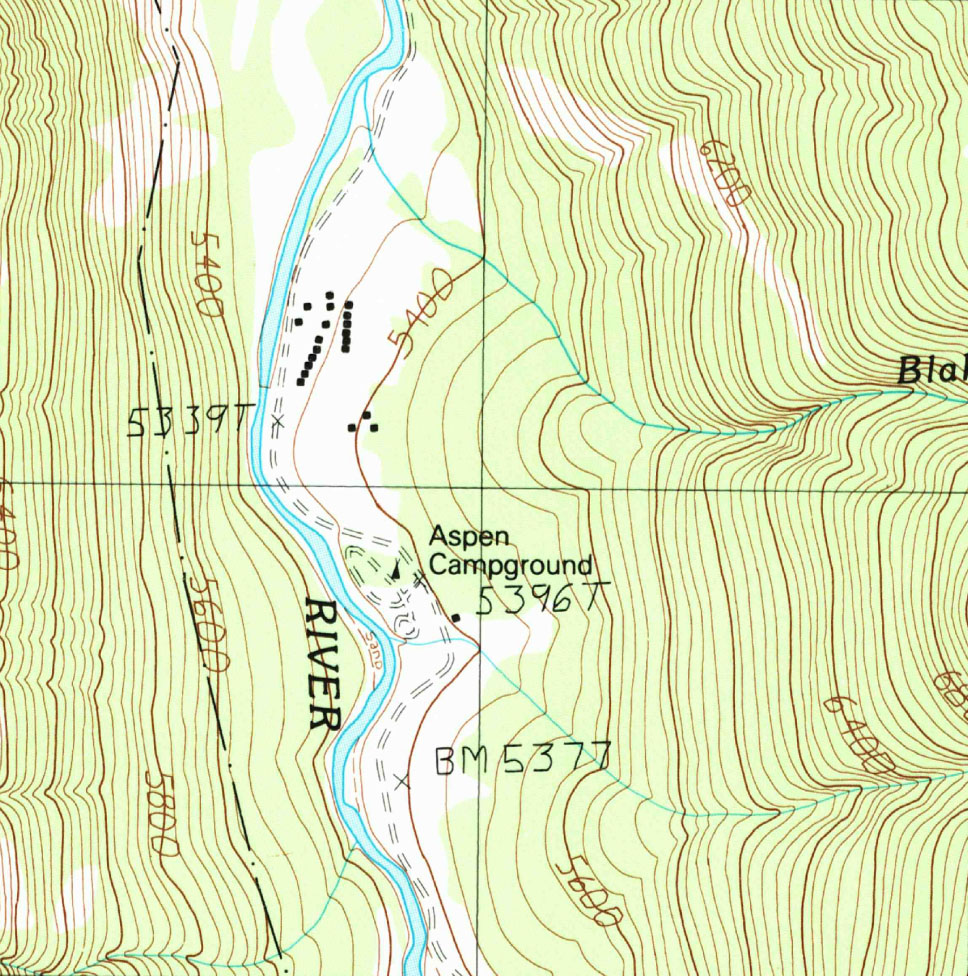
\includegraphics[scale=.65]{figures/MT_ChromeMountain_topo_small.pdf}
%}

Given a function $z=f(x,y)$, we can draw a ``topographical map'' of $f$ by drawing \textbf{level curves} (or, contour lines). A level curve at $z=c$ is a curve in the $x$-$y$ plane such that for all points $(x,y)$ on the curve, $f(x,y) = c$. 

When drawing level curves, it is important that the $c$ values are spaced equally apart as that gives the best insight to how quickly the ``elevation'' is changing. Examples will help one understand this concept.\\

\example{ex_levelcurve1}{Drawing Level Curves}{
Let $\ds f(x,y) = \sqrt{1-\frac{x^2}9-\frac{y^2}4}$. Find the level curves of $f$ for $c=0$, $0.2$, $0.4$, $0.6$, $0.8$ and $1$.}
{Consider first $c=0$. The level curve for $c=0$ is the set of all points $(x,y)$ such that $0=\sqrt{1-\frac{x^2}9-\frac{y^2}4}$. Squaring both sides  gives us
\[
\frac{x^2}9+\frac{y^2}4=1,
\]
an ellipse centred at $(0,0)$ with horizontal major axis of length 6 and minor axis of length 4. Thus for any point $(x,y)$ on this curve, $f(x,y) = 0$.

Now consider the level curve for $c=0.2$
\begin{align*}
0.2 &= \sqrt{1-\frac{x^2}9-\frac{y^2}4}\\
0.04 &= 1-\frac{x^2}9-\frac{y^2}4\\
\frac{x^2}9+\frac{y^2}4 &=0.96\\
\frac{x^2}{8.64}+\frac{y^2}{3.84} &=1.
\end{align*}
This is also an ellipse, where $a = \sqrt{8.64}\approx 2.94$ and $b=\sqrt{3.84}\approx 1.96$.

In general, for $z=c$, the level curve is:
\begin{align*}
c &= \sqrt{1-\frac{x^2}9-\frac{y^2}4}\\
c^2 &= 1-\frac{x^2}9-\frac{y^2}4\\
\frac{x^2}9+\frac{y^2}4 &=1-c^2\\
\frac{x^2}{9(1-c^2)}+\frac{y^2}{4(1-c^2)} &=1,
\end{align*}
ellipses that are decreasing in size as $c$ increases. A special case is when $c=1$; there the ellipse is just the point $(0,0)$. 

The level curves are shown in Figure \ref{fig:levelcurves1}(a). Note how the level curves for $c=0$ and $c=0.2$ are very, very close together: this indicates that $f$ is growing rapidly along those curves.

\mtable{.71}{Graphing the level curves in Example \ref{ex_levelcurve1}.}{fig:levelcurves1}{%
\begin{tabular}{c}
\myincludegraphics{figures/figlevelcurve1b}\\
(a)\\[10pt]
\myincludegraphicsthree{width=150pt,3Dmenu,activate=onclick,deactivate=pageinvisible,
3Droll=0,
3Dortho=0.004999999888241291,
3Dc2c=0.6562340259552002 0.7273486256599426 0.20080043375492096,
3Dcoo=2.348435640335083 -6.5163373947143555 66.12745666503906,
3Droo=129.99999641808185,
3Dlights=Headlamp,add3Djscript=asylabels.js}{width=150pt}{figures/figlevelcurve1}\\
%\myincludegraphics[scale=1.25,trim=3mm 0mm 3mm 0mm,clip]{figures/figlevelcurve1}\\
(b)
\end{tabular}
}

In Figure \ref{fig:levelcurves1}(b), the curves are drawn on a graph of $f$ in space. Note how the elevations are evenly spaced. Near the level curves of $c=0$ and $c=0.2$ we can see that $f$ indeed is growing quickly.
}\\

\example{ex_levelcurves2}{Analyzing Level Curves}{
Let $\ds f(x,y) = \frac{x+y}{x^2+y^2+1}$. Find the level curves for $z=c$.}
{We begin by setting $f(x,y)=c$ for an arbitrary $c$ and seeing if algebraic manipulation of the equation reveals anything significant.
\begin{align*}
\frac{x+y}{x^2+y^2+1} &= c \\
x+y &= c(x^2+y^2+1).
\intertext{We recognize this as a circle, though the center and radius are not yet clear. By completing the square, we can obtain:}
\left(x-\frac{1}{2c}\right)^2+\left(y-\frac1{2c}\right)^2&=\frac{1}{2c^2}-1,
\end{align*}
a circle centred at $\big(1/(2c),1/(2c)\big)$ with radius $\sqrt{1/(2c^2)-1}$, where $\vert c\rvert <1/\sqrt{2}$. The level curves for $c=\pm 0.2,\ \pm 0.4$ and $\pm0.6$ are sketched in Figure \ref{fig:levelcurves2}(a). To help illustrate ``elevation,'' we use thicker lines for $c$ values near 0, and dashed lines indicate where $c<0$. 

There is one special level curve, when $c=0$. The level curve in this situation is $x+y=0$, the line $y=-x$.

In Figure \ref{fig:levelcurves2}(b) we see a graph of the surface. Note how the $y$-axis is pointing away from the viewer to more closely resemble the orientation of the level curves in (a). 

\mtable{.27}{Graphing the level curves in Example \ref{ex_levelcurves2}.}{fig:levelcurves2}{%
\begin{tabular}{c}
\myincludegraphics{figures/figlevelcurve2b}\\
(a)\\[10pt]
%\myincludegraphics[scale=1.2,trim=0mm 5mm 0mm 0mm,clip]{figures/figlevelcurve2}\\
{\myincludegraphicsthree{width=150pt,3Dmenu,activate=onclick,deactivate=pageinvisible,
3Droll=0.25732633644359904,
3Dortho=0.004999999888241291,
3Dc2c=0.5196654200553894 -0.7088789939880371 0.4769051671028137,
3Dcoo=-0.7249413728713989 1.7016432285308838 3.277412176132202,
3Droo=130.00000541214214,
3Dlights=Headlamp,add3Djscript=asylabels.js}{width=150pt}{figures/figlevelcurve2}}\\
(b)
\end{tabular}
}



%\mfigurethree[width=150pt,3Dmenu,activate=onclick,deactivate=pageinvisible,
%3Droll=0,
%3Dc2c=1 -1.5 1,
%3Dcoo=0 0 0,
%3Droo=130,
%3Dortho=.005,
%3Dlights=Headlamp,add3Djscript=asylabels.js]{.4}{Visualizing the solid shown from Example \ref{ex_doublepol4}.}{fig:doublepol4}{figures/figlevelcurve2_3D} 

Seeing the level curves helps us understand the graph. For instance, the graph does not make it clear that one can ``walk'' along the line $y=-x$ without elevation change, though the level curve does.
}\\

\noindent\textbf{\large Functions of Three Variables}\\

We extend our study of multivariable functions to functions of three variables. (One can make a function of as many variables as one likes; we limit our study to three variables.)

\definition{def:multi3}{Function of Three Variables}
{Let $D$ be a subset of $\mathbb{R}^3$. A \textbf{function $f$ of three variables} is a rule that assigns each triple $(x,y,z)$ in $D$ a value $w=f(x,y,z)$ in $\mathbb{R}$. $D$ is the \textbf{domain} of $f$; the set of all outputs of $f$ is the \textbf{range}.
\index{multivariable function}\index{function!of three variables}\index{multivariable function!domain}\index{multivariable function!range}
}

Note how this definition closely resembles that of Definition \ref{def:multi2}.\\

\example{ex_multi3}{Understanding a function of three variables}{
Let $\ds f(x,y,z) =  \frac{x^2+z+3\sin y}{x+2y-z}.$ Evaluate $f$ at the point $(3,0,2)$ and find the domain and range of $f$.}
{$\ds f(3,0,2) = \frac{3^2+2+3\sin 0}{3+2(0)-2} = 11.$

As the domain of $f$ is not specified, we take it to be the set of all triples $(x,y,z)$ for which $f(x,y,z)$ is defined. As we cannot divide by $0$, we find the domain $D$ is 
\[
D = \{(x,y,z)\ |\ x+2y-z\neq 0\}.
\]
We recognize that the set of all points in $\mathbb{R}^3$ that \textit{are not} in $D$ form a plane in space that passes through the origin (with normal vector $\la 1,2,-1\ra$). 

We determine the range $R$ is $\mathbb{R}$; that is, all real numbers are possible outputs of $f$. There is no set way of establishing this. Rather, to get numbers near 0 we can let $y=0$ and choose $z \approx -x^2$. To get numbers of arbitrarily large magnitude, we can let $z\approx x+2y$. 
}\\

%\clearpage
\noindent\textbf{\large Level Surfaces}\\

It is very difficult to produce a meaningful graph of a function of three variables. A function of \textit{one} variable is a \textit{curve} drawn in \textit{2} dimensions; a function of \textit{two} variables is a \textit{surface} drawn in \textit{3} dimensions; a function of \textit{three} variables is a \textit{hypersurface} drawn in \textit{4} dimensions.\index{multivariable function!level surface}\index{level surface}

There are a few techniques one can employ to try to ``picture'' a graph of three variables. One is an analogue of level curves: \textbf{level surfaces}. Given $w=f(x,y,z)$, the level surface at $w=c$ is the surface in space formed by all points $(x,y,z)$ where $f(x,y,z)=c$. \\

\example{ex_multi4}{Finding level surfaces}{
If a point source $S$ is radiating energy, the intensity $I$ at a given point $P$ in space is inversely proportional to the square of the distance between $S$ and $P$. That is, when $S=(0,0,0)$,  $\ds I(x,y,z) = \frac{k}{x^2+y^2+z^2}$ for some constant $k$.

Let $k=1$; find the level surfaces of $I$.}
{We can (mostly) answer this question using ``common sense.'' If energy (say, in the form of light) is emanating from the origin, its intensity will be the same at all points equidistant from the origin. That is, at any point on the surface of a sphere centred at the origin, the intensity should be the same. Therefore, the level surfaces are spheres.

We now find this mathematically. The level surface at $I=c$ is defined by 
\begin{align*}
c &= \frac{1}{x^2+y^2+z^2}.
\intertext{A small amount of algebra reveals}
x^2+y^2+z^2 &= \frac1c.
\end{align*}
Given an intensity $c$, the level surface $I=c$ is a sphere of radius $1/\sqrt{c}$, centred at the origin. 

\mtable{.7}{A table of $c$ values and the corresponding radius $r$ of the spheres of constant value in Example \ref{ex_multi4}.}{fig:multi4}{
\begin{tabular}{cc}
$c$ & $r$ \\ \hline
16. & 0.25 \\
 8. & 0.35 \\
 4. & 0.5 \\
 2. & 0.71 \\
 1. & 1. \\
 0.5 & 1.41 \\
 0.25 & 2. \\
 0.125 & 2.83 \\
 0.0625 & 4. \\
\end{tabular}
}

Figure \ref{fig:multi4} gives a table of the radii of the spheres for given $c$ values. Normally one would use equally spaced $c$ values, but these values have been chosen purposefully. At a distance of 0.25 from the point source, the intensity is 16; to move to a point of half that intensity, one just moves out 0.1 to 0.35 -- not much at all. To again halve the intensity, one moves 0.15, a little more than before.

Note how each time the intensity if halved, the distance required to move away grows. We conclude that the closer one is to the source, the more rapidly the intensity changes.
}\\

\enlargethispage{2\baselineskip}
In the next section we apply the concepts of limits to functions of two or more variables.

\printexercises{exercises/12_01_exercises}

\section{Limits and Continuity of Multivariable Functions}\label{sec:multi_limit}

We continue with the pattern we have established in this text: after defining a new kind of function, we apply calculus ideas to it. The previous section defined functions of two and three variables; this section investigates what it means for these functions to be ``continuous.''

We begin with a series of definitions. We are used to ``open intervals'' such as $(1,3)$, which represents the set of all $x$ such that $1<x<3$,  and ``closed intervals'' such as $[1,3]$, which represents the set of all $x$ such that $1\leq x\leq 3$. We need analogous definitions for open and closed sets in the $x$-$y$ plane.

\definition{def:open}{\parbox[t]{225pt}{Open Disk, Boundary and Interior Points, Open and Closed Sets, Bounded Sets}}
{An \textbf{open disk} $B$ in $\mathbb{R}^2$ centered at $(x_0,y_0)$ with radius $r$ is the set of all points $(x,y)$ such that $\ds\sqrt{(x-x_0)^2+(y-y_0)^2} < r$. \\

Let $S$ be a set of points in $\mathbb{R}^2$. A point $P$ in $\mathbb{R}^2$ is a \textbf{boundary point} of $S$  if all open disks centered at $P$ contain both points in $S$ and points not in $S$.\\

A point $P$ in $S$ is an \textbf{interior point} of $S$ if there is an open disk centered at $P$ that contains only points in $S$. \\

A set $S$ is \textbf{open} if every point in $S$ is an interior point.\\

A set $S$ is \textbf{closed} if it contains all of its boundary points.\\

A set $S$ is \textbf{bounded} if there is an $M>0$ such that the open disk, centered at the origin with radius $M$, contains $S$. A set that is not bounded is \textbf{unbounded}.
\index{open}\index{closed}\index{open disk}\index{closed disk}\index{boundary point}\index{interior point}\index{bounded set}\index{unbounded set}
}

Figure \ref{fig:multilimit_intro} shows several sets in the $x$-$y$ plane. In each set, point $P_1$ lies on the boundary of the set as all open disks centered there contain both points in, and not in, the set. In contrast, point $P_2$ is an interior point for there is an open disk centered there that lies entirely within the set.
\mtable{.6}{Illustrating open and closed sets in the $x$-$y$ plane.}{fig:multilimit_intro}{%
\begin{tabular}{c}
\myincludegraphics{figures/figmultilimit_introa}\\
(a)\\[10pt]
\myincludegraphics{figures/figmultilimit_introb}\\
(b)\\[10pt]
\myincludegraphics{figures/figmultilimit_introc}\\
(c)\\[10pt]
\end{tabular}
}

The set depicted in Figure \ref{fig:multilimit_intro}(a) is a closed set as it contains all of its boundary points. The set in (b) is open, for all of its points are interior points (or, equivalently, it does not contain any of its boundary points). The set in (c) is neither open nor closed as it contains  some of its boundary points.\\


\example{ex_multilimit1}{Determining open/closed, bounded/unbounded}{
Determine if the domain of the function $f(x,y)=\sqrt{1-\frac{x^2}9-\frac{y^2}4}$ is open, closed, or neither, and if it is bounded.}
{This domain of this function was found in Example \ref{ex_multi2} to be $D = \{(x,y)\ |\ \frac{x^2}9+\frac{y^2}4\leq 1\}$, the region \textit{bounded} by the ellipse $\frac{x^2}9+\frac{y^2}4=1$. Since the region includes the boundary (indicated by the use of ``$\leq$''), the set contains all of its boundary points and hence is closed. The region is bounded as a disk of radius 4, centered at the origin, contains $D$.
}\\
\pagebreak

\example{ex_multilimit2}{Determining open/closed, bounded/unbounded}{
Determine if the domain of $f(x,y) = \frac1{x-y}$ is open, closed, or neither.}
{As we cannot divide by 0, we find the domain to be $D = \{(x,y)\ |\ x-y\neq 0\}$. In other words, the domain is the set of all points $(x,y)$ \emph{not} on the line $y=x$. 

\mfigure{.75}{Sketching the domain of the function in Example \ref{ex_multilimit2}.}{fig:multilimit2}{figures/figmultilimit2}
The domain is sketched in Figure \ref{fig:multilimit2}. Note how we can draw an open disk around any point in the domain that lies entirely inside the domain, and also note how the only boundary points of the domain are the points on the line $y=x$. We conclude the domain is an open set. The set is unbounded.
}\\

\noindent\textbf{\large Limits}\\

Recall a pseudo--definition of the limit of a function of one variable: ``$\ds \lim_{x\to c}f(x) = L$'' means that if $x$ is ``really close'' to $c$, then $f(x)$ is ``really close'' to $L$. A similar pseudo--definition holds for functions of two variables. We'll say that 
%\enlargethispage{3\baselineskip}

\begin{center}
``$\ds \lim_{(x,y)\to (x_0,y_0)} f(x,y) = L$'' 
\end{center}
means ``if the point $(x,y)$ is really close to the point $(x_0,y_0)$, then $f(x,y)$ is really close to $L$.'' The formal definition is given below.

\mfigurethree{width=150pt,3Dmenu,activate=onclick,deactivate=onclick,
3Droll=0.12234160136132792,
3Dortho=0.004824123345315456,
3Dc2c=0.9118747115135193 -0.1974218785762787 0.35987377166748047,
3Dcoo=21.82058334350586 66.31769561767578 47.81545639038086,
3Droo=149.99999973566392,
3Dlights=Headlamp,add3Djscript=asylabels.js}{scale=1.25}{.25}{\textbf{Illustrating the definition of a limit.} The open disk in the $x$-$y$ plane has radius $\delta$. Let $(x,y)$ be any point in this disk; $f(x,y)$ is within $\epsilon$ of $L$.}{fig:multilimitdef}{figures/figmultilimit_def}

\definition{def:multilimit}{Limit of a Function of Two Variables}
{Let $S$ be an open set containing $(x_0,y_0)$, and let $f$ be a function of two variables defined on $S$, except possibly at $(x_0,y_0)$. 
%Let $f(x,y)$ be a function of two variables and let $(x_0,y_0)$ be a point in the domain of $f$. 
The \textbf{limit} of $f(x,y)$ as $(x,y)$ approaches $(x_0,y_0)$ is $L$, denoted $$\ds \lim_{(x,y)\to (x_0,y_0)} f(x,y) = L,$$
means that given any $\epsilon>0$, there exists $\delta>0$ such that for all  $(x,y)\neq (x_0,y_0)$, if $(x,y)$ is in the open disk centered at $(x_0,y_0)$ with radius $\delta$, then $|f(x,y) - L|<\epsilon.$
\index{limit!of multivariable function}\index{multivariable function!limit}
}


The concept behind Definition \ref{def:multilimit} is sketched in Figure \ref{fig:multilimitdef}. Given $\epsilon>0$, find $\delta>0$ such that if $(x,y)$ is any point in the open disk centred at $(x_0,y_0)$ in the $x$-$y$ plane with radius $\delta$, then $f(x,y)$ should be within $\epsilon$ of $L$. 

\pagebreak

Computing limits using this definition is rather cumbersome. The following theorem allows us to evaluate limits much more easily.


%\mfigure[scale=1.25]{.77}{\textbf{Illustrating the definition of a limit.} The open disk in the $x$-$y$ plane has radius $\delta$. Let $(x,y)$ be any point in this disk; $f(x,y)$ is within $\epsilon$ of $L$.}{fig:multilimitdef}{figures/figmultilimit_def}


\setboxwidth{0pt}
\theorem{thm:multi_limit_algebra}{Basic Limit Properties of Functions of Two Variables}{%\small
Let $b$, $x_0$, $y_0$, $L$ and $K$ be real numbers,  let $n$ be a positive integer, and let $f$ and $g$ be functions with the following limits:
$$\lim_{(x,y)\to (x_0,y_0)}f(x,y) = L \quad \text{\ and\ } \lim_{(x,y)\to (x_0,y_0)} g(x,y) = K.$$
The following limits hold.
\index{limit!of multivariable function}\index{limit!properties}\index{multivariable function!limit}
\begin{enumerate}
\item \parbox{80pt}{Constants:} $\displaystyle \lim_{(x,y)\to (x_0,y_0)} b = b$
\item	\parbox{80pt}{Identity }	$\displaystyle \lim_{(x,y)\to (x_0,y_0)} x = x_0$;\qquad $\displaystyle \lim_{(x,y)\to (x_0,y_0)} y = y_0$
\item	\parbox{80pt}{Sums/Differences:} $\displaystyle \lim_{(x,y)\to (x_0,y_0)}\big(f(x,y)\pm g(x,y)\big) = L\pm K$
\item	\parbox{80pt}{Scalar Multiples:}	$\displaystyle \lim_{(x,y)\to (x_0,y_0)} b\cdot f(x,y) = bL$
\item	\parbox{80pt}{Products:}	$\displaystyle \lim_{(x,y)\to (x_0,y_0)} f(x,y)\cdot g(x,y) = LK$
\item	\parbox{80pt}{Quotients:} $\displaystyle \lim_{(x,y)\to (x_0,y_0)} f(x,y)/g(x,y) = L/K$, ($K\neq 0)$
\item	\parbox{80pt}{Powers:} 	$\displaystyle \lim_{(x,y)\to (x_0,y_0)} f(x,y)^n = L^n$
%\item	\parbox{80pt}{Roots:}		\parbox[t]{185pt}{$\displaystyle \lim_{(x,y)\to (x_0,y_0)} \sqrt[n]{f(x,y)} = \sqrt[n]{L}$}% \qquad \small (if $n$ is even then $L$ must be greater than 0; when $n$ is odd, it is true for all $L$.)}

\end{enumerate}
}
\restoreboxwidth

This theorem, combined with Theorems \ref{thm:poly_rat} and \ref{thm:lim_continuous} of Section \ref{sec:limit_analytically}, allows us to evaluate many limits.\\

\example{ex_multilimit3}{Evaluating a limit}{
Evaluate the following limits:
$$1. \lim_{(x,y)\to (1,\pi)} \frac yx + \cos(xy) \qquad\qquad 2. \lim_{(x,y)\to (0,0)} \frac{3xy}{x^2+y^2}$$
}
{\begin{enumerate}
	\item The aforementioned theorems allow us to simply evaluate $y/x+\cos(xy)$ when $x=1$ and $y=\pi$. If an indeterminate form is returned, we must do more work to evaluate the limit; otherwise, the result is the limit. Therefore
	\begin{align*}
	\lim_{(x,y)\to (1,\pi)} \frac yx + \cos(xy)  &= \frac\pi{1}+\cos \pi \\
		&= \pi -1.
	\end{align*}
	\item		We attempt to evaluate the limit by substituting 0 in for $x$ and $y$, but the result is the indeterminate form ``$0/0$.'' To evaluate this limit, we must ``do more work,'' but we have not yet learned what ``kind'' of work to do. Therefore we cannot yet evaluate this limit.
\end{enumerate}
\vskip -1.5\baselineskip
}\\

When dealing with functions of a single variable we also considered one--sided limits and stated
$$\lim_{x\to c}f(x) = L \quad\text{ if, and only if,}\quad \lim_{x\to c^+}f(x) =L \quad\textbf{ and}\quad \lim_{x\to c^-}f(x) =L.$$
That is, the limit is $L$ if and only if $f(x)$ approaches $L$ when $x$ approaches $c$ from \textbf{either} direction, the left or the right.

In the plane, there are infinite directions from which $(x,y)$ might approach $(x_0,y_0)$. In fact, we do not have to restrict ourselves to approaching $(x_0,y_0)$ from a particular direction, but rather we can approach that point along a path that is not a straight line. It is possible to arrive at different limiting values by approaching $(x_0,y_0)$ along different paths. If this happens, we say that $\ds \lim_{(x,y)\to(x_0,y_0) } f(x,y)$ does not exist (this is analogous to the left and right hand limits of single variable functions not being equal).

Our theorems tell us that we can evaluate most limits quite simply, without worrying about  paths. When indeterminate forms arise, the limit may or may not exist. If it does exist, it can be difficult to prove this as we need to show the same limiting value is obtained regardless of the path chosen. The case where the limit does not exist is often easier to deal with, for we can often pick two paths along which the limit is different.\\

%it can be difficult to show that the limit exists, for we need to show that the same limiting value is obtained regardless of the path taken.  we can often evaluate the limit along specific paths. If any of these limits differ, we say that \emph{the} limit does not exist.\\

\example{ex_multilimit4}{Showing limits do not exist}{
\begin{enumerate}
	\item Show $\ds \lim_{(x,y)\to (0,0)} \frac{3xy}{x^2+y^2}$ does not exist by finding the limits along the lines $y=mx$.
	\item	Show $\ds \lim_{(x,y)\to (0,0)} \frac{\sin(xy)}{x+y}$ does not exist by finding the limit along the path $y=-\sin x$. 	
\end{enumerate}
}
{\begin{enumerate}
	\item Evaluating $\ds \lim_{(x,y)\to (0,0)} \frac{3xy}{x^2+y^2}$ along the lines $y=mx$ means replace all $y$'s with $mx$ and evaluating the resulting limit:
	\begin{align*}
	\lim_{(x,mx)\to (0,0)} \frac{3x(mx)}{x^2+(mx)^2} &=\lim_{x\to 0} \frac{3mx^2}{x^2(m^2+1)}\\
				&= \lim_{x\to 0} \frac{3m}{m^2+1}\\
				&= \frac{3m}{m^2+1}.
	\end{align*}
	While the limit exists for each choice of $m$, we get a \emph{different} limit for each choice of $m$. That is, along different lines we get differing limiting values, meaning \emph{the} limit does not exist.
	
	\item		Let $f(x,y) = \frac{\sin(xy)}{x+y}$. We are to show that $\ds \lim_{(x,y)\to (0,0)} f(x,y)$ does not exist by finding the limit along the path $y=-\sin x$. First, however, consider the limits found along the lines $y=mx$ as done above.
	\begin{align*}
	\lim_{(x,mx)\to (0,0)} \frac{\sin\big(x(mx)\big)}{x+mx} &= \lim_{x\to 0} \frac{\sin (mx^2)}{x(m+1)} \\
	&= \lim_{x\to 0} \frac{\sin(mx^2)}{x}\cdot\frac1{m+1}.
	\end{align*}
	By applying L'H\^opital's Rule, we can show this limit is 0 \emph{except} when $m=-1$, that is, along the line $y=-x$. This line is not in the domain of $f$, so we have found the following fact: along every line $y=mx$ in the domain of $f$, $\ds \lim_{(x,y)\to(0,0)} f(x,y)=0$. %Along this line, $f(x,y)$ is not defined, so it stands to reason that a limit along this line does not exist.
%\drawexampleline
	
	Now consider the limit along the path $y=-\sin x$:
	\begin{align*}
	\lim_{(x,-\sin x)\to (0,0)} \frac{\sin\big(-x\sin x\big)}{x-\sin x} &= \lim_{x\to0} \frac{\sin\big(-x\sin x\big)}{x-\sin x}
	\end{align*}
	Now apply L'H\^opital's Rule twice:
	\small
	\begin{align*}
	 \quad &= \lim_{x\to 0}\frac{\cos\big(-x\sin x\big)(-\sin x-x\cos x)}{1-\cos x} \quad \left(\text{``}= 0/0\text{''}\right)\\
	&= \lim_{x\to 0}\frac{-\sin\big(-x\sin x\big)(-\sin x-x\cos x)^2+\cos\big(-x\sin x\big)(-2\cos x+x\sin x)}{\sin x}\\
	&= \text{``2/0''} \Rightarrow \text{the limit does not exist.}
	\end{align*}
	\normalsize
Step back and consider what we have just discovered. Along any line $y=mx$ in the domain of the $f(x,y)$, the limit is 0. However, along the path $y=-\sin x$, which lies in the domain of  $f(x,y)$ for all $x\neq 0$, the limit does not exist. Since the limit is not the same along every path to $(0,0)$, we say $\ds \lim_{(x,y)\to (0,0)}\frac{\sin(xy)}{x+y}$ does not exist.
\end{enumerate}
\vskip -1.5\baselineskip
}\\

\example{ex_multilimit5}{Finding a limit}{
Let $\ds f(x,y) = \frac{5x^2y^2}{x^2+y^2}$. Find $\ds\lim_{(x,y)\to (0,0)}  f(x,y) .$
}
{It is relatively easy to show that along any line $y=mx$, the limit is 0. This is not enough to prove that the limit exists, as demonstrated in the previous example, but it tells us that if the limit does exist then it must be 0.

To prove the limit is 0, we apply Definition \ref{def:multilimit}. Let $\epsilon >0$ be given. We want to find $\delta >0$ such that if $\sqrt{(x-0)^2+(y-0)^2} <\delta$, then $|f(x,y)-0| <\epsilon$.

Set $\delta < \sqrt{\epsilon/5}$. Note that $\ds \left|\frac{5y^2}{x^2+y^2}\right| <5$ for all $(x,y)\neq (0,0)$, and that if $\sqrt{x^2+y^2} <\delta$, then $x^2<\delta^2$.

Let $\sqrt{(x-0)^2+(y-0)^2} = \sqrt{x^2+y^2}<\delta$. Consider $|f(x,y)-0|$:
\begin{align*}
|f(x,y)-0| &= \left|\frac{5x^2y^2}{x^2+y^2}-0\right| \\
				&= \left|x^2\cdot\frac{5y^2}{x^2+y^2}\right|\\
				&< \delta^2\cdot 5 \\
				&< \frac{\epsilon}{5}\cdot 5 \\
				&= \epsilon.
\end{align*}
Thus if $\sqrt{(x-0)^2+(y-0)^2}<\delta$ then $|f(x,y)-0|<\epsilon$, which is what we wanted to show. Thus $\ds \lim_{(x,y)\to(0,0)} \frac{5x^2y^2}{x^2+y^2} = 0$.
}\\
%\pagebreak

\noindent\textbf{\large Continuity}\\

Definition \ref{def:continuous} defines what it means for a function of one variable to be continuous. In brief, it meant that the graph of the function did not have breaks, holes, jumps, etc. We define continuity for functions of two variables in a similar way as we did for functions of one variable.

\definition{def:multi_continuous}{Continuous}
{Let a function $f(x,y)$ be defined on an open disk $B$ containing the point $(x_0,y_0)$. 

\begin{enumerate}
	\item $f$ is \textbf{continuous} at $(x_0,y_0)$ if $\ds\lim_{(x,y)\to(x_0,y_0)} f(x,y) = f(x_0,y_0)$.
	\index{continuous function}\index{multivariable function!continuity}
	\item	$f$ is \textbf{continuous on $B$} if $f$ is continuous at all points in $B$. If $f$ is continuous at all points in $\mathbb{R}^2$, we say that $f$ is \textbf{continuous everywhere}.
\end{enumerate}
}

\example{ex_multicont1}{Continuity of a function of two variables}{
Let $\ds f(x,y) = \left\{ \begin{array}{rl} \frac{\cos y\sin x}{x} & x\neq 0 \\
																						\cos y & x=0
													\end{array} \right.$. Is $f$ continuous at $(0,0)$? Is $f$ continuous everywhere?
}
{To determine if $f$ is continuous at $(0,0)$, we need to compare $\ds\lim_{(x,y)\to (0,0)} f(x,y)$ to $f(0,0)$. 

Applying the definition of $f$, we see that $f(0,0) = \cos 0 = 1$. 

We now consider the limit $\ds \lim_{(x,y)\to (0,0)} f(x,y)$. Substituting $0$ for $x$ and $y$ in $(\cos y\sin x)/x$ returns the indeterminate form ``0/0'', so we need to do more work to evaluate this limit.

Consider two related limits: $\ds \lim_{(x,y)\to (0,0)} \cos y$ and $\ds \lim_{(x,y)\to(0,0)} \frac{\sin x}x$. The first limit does not contain $x$, and since $\cos y$ is continuous, $$\ds \lim_{(x,y)\to (0,0)} \cos y =\lim_{y\to 0} \cos y = \cos 0 = 1.$$

The second limit does not contain $y$. By Theorem \ref{thm:special_limits} we can say
$$\lim_{(x,y)\to (0,0)} \frac{\sin x}{x} = \lim_{x\to 0} \frac{\sin x}{x} = 1.$$
Finally, Theorem \ref{thm:multi_limit_algebra} of this section states that we can combine these two limits as follows:
\begin{align*}
\lim_{(x,y)\to (0,0)} \frac{\cos y\sin x}{x} &= \lim_{(x,y)\to (0,0)} (\cos y)\left(\frac{\sin x}{x}\right) \\ 
&=\left(\lim_{(x,y)\to (0,0)} \cos y\right)\left(\lim_{(x,y)\to (0,0)} \frac{\sin x}{x}\right) \\
  &= (1)(1)\\
	&=1.
\end{align*}

We have found that $\ds \lim_{(x,y)\to (0,0)} \frac{\cos y\sin x}{x} = f(0,0)$, so $f$ is continuous at $(0,0)$.

A similar analysis shows that $f$ is continuous at all points in $\mathbb{R}^2$. As long as $x\neq0$, we can evaluate the limit directly; when $x=0$, a similar analysis shows that the limit is $\cos y$. Thus we can say that $f$ is continuous everywhere. A graph of $f$ is given in Figure \ref{fig:multicont1}. Notice how it has no breaks, jumps, etc.
\mfigurethree{width=150pt,3Dmenu,activate=onclick,deactivate=onclick,
3Droll=1.3976649182325884,
3Dortho=0.005226649809628725,
3Dc2c=0.6559564471244812 0.554935097694397 0.5116328597068787,
3Dcoo=-1.2457355260849 0.0923926830291748 4.189182281494141,
3Droo=129.99999868169073,
3Dlights=Headlamp,add3Djscript=asylabels.js}{scale=1.25}{.5}{A graph of $f(x,y)$ in Example \ref{ex_multicont1}.}{fig:multicont1}{figures/figmulticont1}
%\mfigure[scale=1.25]{.8}{A graph of $f(x,y)$ in Example \ref{ex_multicont1}.}{fig:multicont1}{figures/figmulticont1}
}\\

The following theorem is very similar to Theorem \ref{thm:continuity_algebra}, giving us ways to combine continuous functions to create other continuous functions.

\theorem{thm:multi_continuous_prop}{Properties of Continuous Functions}
{Let $f$ and $g$ be continuous on an open disk $B$, let $c$ be a real number, and let $n$ be a positive integer. The following functions are continuous on $B$.
\index{continuous function!properties}\index{multivariable function!continuity}
		\begin{enumerate}
		\item		\parbox{80pt}{Sums/Differences:}	$f\pm g$
		\item		\parbox{80pt}{Constant Multiples:}	$c\cdot f$
		\item		\parbox{80pt}{Products:}	$f\cdot g$
		\item		\parbox{80pt}{Quotients:}	$f/g$ \qquad {\small (as longs as $g\neq 0$ on $B$)}
		\item		\parbox{80pt}{Powers:}	$f\,^n$
		\item		\parbox{80pt}{Roots:}	$\sqrt[n]{f}$ \qquad \parbox[t]{150pt}{\small (if $n$ is even then $f\geq 0$ on $B$; if $n$ is odd, then true for all values of $f$ on $B$.)}
		\item		\parbox{80pt}{Compositions:}\parbox[t]{185pt}{Adjust the definitions of $f$ and $g$ to: Let $f$ be continuous on $B$, where the range of $f$ on $B$ is $J$, and let $g$ be a single variable function that is continuous on $J$. Then $g\circ f$, i.e., $g(f(x,y))$, is continuous on $B$.}
		\end{enumerate}
}
\enlargethispage{\baselineskip}

\example{ex_multicont2}{Establishing continuity of a function}{
Let $f(x,y) = \sin (x^2\cos y)$. Show $f$ is continuous everywhere.}
{We will apply both Theorems \ref{thm:continuity_algebra} and \ref{thm:multi_continuous_prop}. Let $f_1(x,y) = x^2$. Since $y$ is not actually used in the function, and polynomials are continuous (by Theorem \ref{thm:continuity_algebra}), we conclude $f_1$ is continuous everywhere. A similar statement can be made about $f_2(x,y) = \cos y$. Part 3 of Theorem \ref{thm:multi_continuous_prop} states that $f_3=f_1\cdot f_2$ is continuous everywhere, and Part 7 of the theorem states the composition of sine with $f_3$ is continuous: that is, $\sin (f_3) = \sin(x^2\cos y)$ is continuous everywhere.
}\\
\pagebreak

\noindent\textbf{\large Functions of Three Variables}\\

The definitions and theorems given in this section can be extended in a natural way to definitions and theorems about functions of three (or more) variables. We cover the key concepts here; some terms from Definitions \ref{def:open} and \ref{def:multi_continuous} are not redefined but their analogous meanings should be clear to the reader.

\setboxwidth{20pt}
\definition{def:multi3defs}{Open Balls, Limit, Continuous}
{ 
\begin{enumerate}
\item An \textbf{open ball} in $\mathbb{R}^3$ centered at $(x_0,y_0,z_0)$ with radius $r$ is the set of all points $(x,y,z)$ such that $\sqrt{(x-x_0)^2+(y-y_0)^2+(z-z_0)^2} = r$.
\index{multivariable function!limit}\index{limit!of multivariable function}\index{multivariable function!continuity}\index{open ball}
\\

\item Let $D$ be an open set in $\mathbb{R}^3$ containing $(x_0,y_0,z_0)$, and let $f(x,y,z)$ be a function of three variables defined on $D$, except possibly at  $(x_0,y_0,z_0)$. The \textbf{limit} of $f(x,y,z)$ as $(x,y,z)$ approaches $(x_0,y_0,z_0)$ is $L$, denoted 
$$\lim_{(x,y,z)\to (x_0,y_0,z_0)} f(x,y,z) = L,$$
means that given any $\epsilon >0$, there is a $\delta >0$ such that for all  $(x,y,z)\neq(x_0,y_0,z_0)$, if $(x,y,z)$ is in the open ball centered at $(x_0,y_0,z_0)$ with radius $\delta$, then $|f(x,y,z) - L|< \epsilon$.\\

\item Let $f(x,y,z)$ be defined on an open ball $B$ containing $(x_0,y_0,z_0)$. $f$ is \textbf{continuous} at $(x_0,y_0,z_0)$ if $\ds \lim_{(x,y,z)\to (x_0,y_0,z_0)} f(x,y,z) = f(x_0,y_0,z_0)$.
\end{enumerate}
}
\restoreboxwidth

These definitions can also be extended naturally to apply to functions of four or more variables. Theorem \ref{thm:multi_continuous_prop} also applies to function of three or more variables, allowing us to say that the function $$\ds f(x,y,z) = \frac{e^{x^2+y}\sqrt{y^2+z^2+3}}{\sin (xyz)+5}$$ is continuous everywhere.

When considering single variable functions, we studied limits, then continuity, then the derivative. In our current study of multivariable functions, we have studied limits and continuity. In the next section we study derivation, which takes on a slight twist as we are in a multivarible context.

\printexercises{exercises/12_02_exercises}
\section{Partial Derivatives}\label{sec:partial_derivatives}

Let $y$ be a function of $x$. We have studied in great detail the derivative of $y$ with respect to $x$, that is, $\frac{dy}{dx}$, which measures the rate at which $y$ changes with respect to $x$. Consider now $z=f(x,y)$. It makes sense to want to know how $z$ changes with respect to $x$ and/or $y$. This section begins our investigation into these rates of change.

Consider the function $z=f(x,y) = x^2+2y^2$, as graphed in Figure \ref{fig:partialintro}(a). By fixing $y=2$, we focus our attention to all points on the surface where the $y$-value is 2, shown in both parts (a) and (b) of the figure. These points form a curve in space: $z = f(x,2) = x^2+8$ which is a function of just one variable. We can take the derivative of $z$ with respect to $x$ along this curve and find equations of tangent lines, etc. 

\mtable{.68}{By fixing $y=2$, the surface $f(x,y) = x^2+2y^2$ is a curve in space.}{fig:partialintro}
{\begin{tabular}{c}
\myincludegraphicsthree{width=125pt,3Dmenu,activate=onclick,deactivate=onclick,
3Droll=1.320775024146522,
3Dortho=0.004999999888241291,
3Dc2c=0.6570873856544495 0.6839641332626343 0.31690558791160583,
3Dcoo=-3.0739071369171143 -0.40104401111602783 58.57058334350586,
3Droo=129.99999696026478,
3Dlights=Headlamp,add3Djscript=asylabels.js}{scale=1.25,trim = 2mm 2mm 2mm 2mm,clip}{figures/figpartialintro}\\[10pt]
%\myincludegraphics[scale=1.25,trim = 2mm 2mm 2mm 2mm,clip]{figures/figpartialintro}\\[10pt]
(a)\\[5pt]
\myincludegraphicsthree{width=125pt,3Dmenu,activate=onclick,deactivate=onclick,
3Droll=1.320775024146522,
3Dortho=0.004999999888241291,
3Dc2c=0.6570873856544495 0.6839641332626343 0.31690558791160583,
3Dcoo=-3.0739071369171143 -0.40104401111602783 58.57058334350586,
3Droo=129.99999696026478,
3Dlights=Headlamp,add3Djscript=asylabels.js}{scale=1.25,trim = 2mm 2mm 2mm 2mm,clip}{figures/figpartialintrob}
%\myincludegraphics[scale=1.25,trim = 2mm 2mm 2mm 2mm,clip]{figures/figpartialintrob}\\[10pt]
(b)
\end{tabular}
}

The key notion to extract from this example is: by treating $y$ as  constant (it does not vary) we can consider how $z$ changes with respect to $x$. In a similar fashion, we can hold $x$ constant and consider how $z$ changes with respect to $y$. This is the underlying principle of \textbf{partial derivatives}. We state the formal, limit--based definition first, then show how to compute these partial derivatives without directly taking limits.

%\enlargethispage{4\baselineskip}
\definition{def:partial_derivative}{Partial Derivative}
{Let $z=f(x,y)$ be a continuous function on an open set $S$ in $\mathbb{R}^2$.
\begin{enumerate}
	\item The \textbf{partial derivative of $f$ with respect to $x$} is:
	$$f_x(x,y) = \lim_{h\to 0} \frac{f(x+h,y) - f(x,y)}h.$$
	%Alternate notations for $\frac{\partial z}{\partial x}$ include: $\ds\frac{\partial}{\partial x}f(x,y),\ f_x(x,y),\ \text{and}\ z_x.$
	\item The \textbf{partial derivative of $f$ with respect to $y$} is:
	$$f_y(x,y) = \lim_{h\to 0} \frac{f(x,y+h) - f(x,y)}h.$$
	
	%\item		If $f_x$ and $f_y$ are continuous on $S$, then $f$ is \textbf{differentiable} on $S$.\footnote{This definition of differentiability is mathematically ``weak'' but easy to understand; see Section \ref{sec:total_differential} for a stronger definition that is less intuitive.}
	\end{enumerate}
	\index{partial derivative}\index{derivative!partial}
}
\mnote{.35}{Alternate notations for $f_x(x,y)$ include: $$\frac{\partial}{\partial x}f(x,y),\ \ \frac{\pf}{\px},\ \ \frac{\pz}{\px},\ \ \text{and}\ z_x,$$ with similar notations for $f_y(x,y).$ For ease of notation, $f_x(x,y)$ is often abbreviated $f_x$.}

\example{ex_partial1}{Computing partial derivatives with the limit definition}{
Let $f(x,y) = x^2y + 2x+y^3$. Find $f_x(x,y)$ using the limit definition.}
{Using Definition \ref{def:partial_derivative}, we have:
\begin{align*}
f_x(x,y) &= \lim_{h\to 0} \frac{f(x+h,y) - f(x,y)}{h} \\
				&= \lim_{h\to 0} \frac{(x+h)^2y+2(x+h)+y^3 - (x^2y+2x+y^3)}{h}\\
				&= \lim_{h\to 0} \frac{(x^2y+2xhy+h^2y+2x+2h+y^3-(x^2y+2x+y^3)}{h}\\
				&= \lim_{h\to 0} \frac{2xhy+h^2y+2h}{h}\\
				&=\lim_{h\to 0} 2xy+hy+2\\
				&= 2xy+2.
\end{align*}
We have found $f_x(x,y) = 2xy+2$.
}\\

Example \ref{ex_partial1} found a partial derivative using the formal, limit--based definition. Using limits is not necessary, though, as we can rely on our previous knowledge of derivatives to compute partial derivatives easily. When computing $f_x(x,y)$, we hold $y$ fixed -- it does not vary. Therefore we can compute the derivative with respect to $x$ by treating $y$ as a constant or coefficient. 

Just as $\frac{d}{dx}\big(5x^2\big) = 10x$, we compute $\frac{\partial}{\px}\big(x^2y\big) = 2xy$. Here we are treating $y$ as a coefficient.

Just as $\frac{d}{dx}\big(5^3\big) = 0$, we compute $\frac{\partial}{\px}\big(y^3\big) = 0.$ Here we are treating $y$ as a constant. More examples will help make this clear.\\

\example{ex_partial2}{Finding partial derivatives}{
Find $f_x(x,y)$ and $f_y(x,y)$ in each of the following.
\begin{enumerate}
	\item $f(x,y) = x^3y^2+ 5y^2-x+7$
	\item	$f(x,y) = \cos(xy^2)+\sin x$
	\item	$f(x,y) = e^{x^2y^3}\sqrt{x^2+1}$
\end{enumerate} 
}
{\begin{enumerate}
	\item We have $f(x,y) = x^3y^2+ 5y^2-x+7$.\\
	Begin with $f_x(x,y)$. Keep $y$ fixed, treating it as a constant or coefficient, as appropriate:
	$$f_x(x,y) = 3x^2y^2-1.$$ Note how the $5y^2$ and $7$ terms go to zero.
	
	To compute $f_y(x,y)$, we hold $x$ fixed:
	$$f_y(x,y) = 2x^3y+10y.$$ Note how the $-x$ and $7$ terms go to zero.
	
	\item We have $f(x,y) = \cos(xy^2)+\sin x$.\\
	Begin with $f_x(x,y)$. We need to apply the Chain Rule with the cosine term; $y^2$ is the coefficient of the $x$-term inside the cosine function.
	$$f_x(x,y) = -\sin(xy^2)(y^2)+\cos x = -y^2\sin(xy^2)+\cos x.$$
	To find $f_y(x,y)$, note that $x$ is the coefficient of the $y^2$ term inside of the cosine term; also note that since $x$ is fixed, $\sin x$ is also fixed, and we treat it as a constant.
	$$f_y(x,y) = -\sin(xy^2)(2xy) = -2xy\sin(xy^2).$$
	
	\item		We have $f(x,y) = e^{x^2y^3}\sqrt{x^2+1}$.\\
	Beginning with $f_x(x,y)$, note how we need to apply the Product Rule. 
	\begin{align*}
	f_x(x,y) &= e^{x^2y^3}(2xy^3)\sqrt{x^2+1} + e^{x^2y^3}\frac12\big(x^2+1\big)^{-1/2} \\
					&= 2xy^3e^{x^2y^3}+\frac{e^{x^2y^3}}{2\sqrt{x^2+1}}.
	\end{align*}
	Note that when finding $f_y(x,y)$ we do not have to apply the Product Rule; since $\sqrt{x^2+1}$ does not contain $y$, we treat it as fixed and hence becomes a coefficient of the $e^{x^2y^3}$ term.
	$$f_y(x,y) = e^{x^2y^3}(3x^2y^2)\sqrt{x^2+1} = 3x^2y^2e^{x^2y^3}\sqrt{x^2+1}.$$
\end{enumerate}
\vskip-1.5\baselineskip
}\\

We have shown \textit{how} to compute a partial derivative, but it may still not be clear what a partial derivative \textit{means}. Given $z=f(x,y)$, $f_x(x,y)$ measures the rate at which $z$ changes as only $x$ varies: $y$ is held constant. \index{partial derivative!meaning}

Imagine standing in a rolling meadow, then beginning to walk due east. Depending on your location, you might walk up, sharply down, or perhaps not change elevation at all. This is similar to measuring $z_x$: you are moving only east (in the ``$x$''-direction) and not north/south at all. Going back to your original location, imagine now walking due north (in the ``$y$''-direction). Perhaps walking due north does not change your elevation at all. This is analogous to $z_y=0$: $z$ does not change with respect to $y$. We can see that $z_x$ and $z_y$ do not have to be the same, or even similar, as it is easy to imagine circumstances where walking east means you walk downhill, though walking north makes you walk uphill. 

The following example helps us visualize this more.\\

\example{ex_partial3}{Evaluating partial derivatives}{
Let $z=f(x,y)=-x^2-\frac12y^2+xy+10$. Find $f_x(2,1)$ and $f_y(2,1)$ and interpret their meaning.
}
{We begin by computing $f_x(x,y) = -2x+y$ and $f_y(x,y) = -y+x$. Thus
$$f_x(2,1) = -3 \quad \text{and}\quad f_y(2,1) = 1.$$
It is also useful to note that $f(2,1) = 7.5$. What does each of these numbers mean?

Consider $f_x(2,1)=-3$, along with Figure \ref{fig:partial3}(a). If one ``stands'' on the surface at the point $(2,1,7.5)$ and moves parallel to the $x$-axis (i.e., only the $x$-value changes, not the $y$-value), then the instantaneous rate of change is $-3$. Increasing the $x$-value will decrease the $z$-value; decreasing the $x$-value will increase the $z$-value.

\mtable{.65}{Illustrating the meaning of partial derivatives.}{fig:partial3}{%
\begin{tabular}{c}
\myincludegraphicsthree{width=150pt,3Dmenu,activate=onclick,deactivate=onclick,
3Droll=0.,
3Dortho=0.004999999888241291,
3Dc2c=0.6528097987174988 0.6841705441474915 0.3251922130584717,
3Dcoo=7.158430576324463 9.488722801208496 72.96935272216797,
3Droo=129.9999938624484,
3Dlights=Headlamp,add3Djscript=asylabels.js}{scale=1.25,trim=0mm 5mm 0mm 0mm,clip}{figures/figpartial3a}\\
%\myincludegraphics[scale=1.25,trim=0mm 5mm 0mm 0mm,clip]{figures/figpartial3a}\\
(a)\\[10pt]
\myincludegraphicsthree{width=150pt,3Dmenu,activate=onclick,deactivate=onclick,
3Droll=0.,
3Dortho=0.004999999888241291,
3Dc2c=0.6528097987174988 0.6841705441474915 0.3251922130584717,
3Dcoo=7.158430576324463 9.488722801208496 72.96935272216797,
3Droo=129.9999938624484,
3Dlights=Headlamp,add3Djscript=asylabels.js}{scale=1.25,trim=0mm 5mm 0mm 0mm,clip}{figures/figpartial3b}\\
%\myincludegraphics[scale=1.25,trim=0mm 5mm 0mm 0mm,clip]{figures/figpartial3b}\\
(b)
\end{tabular}
}

Now consider $f_y(2,1)=1$, illustrated in Figure \ref{fig:partial3}(b). Moving along the curve drawn on the surface, i.e., parallel to the $y$-axis and not changing the $x$-values, increases the $z$-value instantaneously at a rate of 1. Increasing the $y$-value by 1 would increase the $z$-value by approximately 1.

Since the magnitude of $f_x$ is greater than the magnitude of $f_y$ at $(2,1)$, it is ``steeper'' in the $x$-direction than in the $y$-direction.
}\\

\pagebreak

\noindent\textbf{\large Second Partial Derivatives}\\

Let $z=f(x,y)$. We have learned to find the partial derivatives $f_x(x,y)$ and $f_y(x,y)$, which are each functions of $x$ and $y$. Therefore we can take partial derivatives of them, each with respect to $x$ and $y$. We define these ``second partials'' along with the notation, give examples, then discuss their meaning.

\definition{def:second_partial}{Second Partial Derivative, Mixed Partial Derivative}
{Let $z=f(x,y)$ be continuous on an open set $S$.
\begin{enumerate}
	\item The \textbf{second partial derivative of $f$ with respect to $x$ then $x$} is $$\frac{\partial}{\partial x}\left(\frac{\partial f}{\px}\right) = \frac{\partial^2 f}{\px^2} = \big(\,f_x\,\big)_x = f_{xx}$$

\item The \textbf{second partial derivative of $f$ with respect to $x$ then $y$} is $$\frac{\partial}{\partial y}\left(\frac{\partial f}{\px}\right) = \frac{\partial^2f}{\py\px} = \big(\,f_x\,\big)_y = f_{xy}$$

%\item The \textbf{second partial derivative of $f$ with respect to $y$ then $y$} is $$\frac{\partial}{\partial y}\left(\frac{\partial f}{\py}\right) = \frac{\partial^2 f}{\py^2} = \big(\,f_y\,\big)_y= f_{yy}$$
%
%\item The \textbf{second partial derivative of $f$ with respect to $y$ then $x$} is $$\frac{\partial}{\partial x}\left(\frac{\partial f}{\py}\right) = \frac{\partial^2f}{\px\py} = \big(\,f_y\,\big)_x = f_{yx}$$

\end{enumerate}

Similar definitions hold for $\ds \frac{\partial^2f}{\py^2} = f_{yy}$ and $\ds \frac{\partial^2f}{\px\py} = f_{yx}$. \\

The second partial derivatives $f_{xy}$ and $f_{yx}$ are \textbf{mixed partial derivatives}.
\index{partial derivative!mixed}\index{partial derivative!second derivative}\index{derivative!mixed partial}
}

The notation of second partial derivatives gives some insight into the notation of the second derivative of a function of a single variable. If $y=f(x)$, then $\ds \fp'(x) = \frac{d^2 y}{dx^2}$. The ``$d^2y$'' portion means ``take the derivative of $y$ twice,'' while ``$dx^2$'' means ``with respect to $x$ both times.'' When we only know of functions of a single variable, this latter phrase seems silly: there is only one variable to take the derivative with respect to. Now that we understand functions of multiple variables, we see the importance of specifying which variables we are referring to.\\

\mnote{.7}{\textbf{Note:} The terms in Definition \ref{def:second_partial} all depend on limits, so each definition comes with the caveat ``where the limit exists.''} 


\example{ex_partial6}{Second partial derivatives}{
For each of the following, find all six first and second partial derivatives. That is, find 
$$f_x,\quad f_y,\quad f_{xx},\quad f_{yy},\quad f_{xy}\quad \text{and}\quad f_{yx}\,.$$
\begin{enumerate}
	\item $f(x,y) = x^3y^2 + 2xy^3+\cos x$
	\item	$\ds f(x,y) = \frac{x^3}{y^2}$
	\item	$f(x,y)=e^{x}\sin(x^2y)$
\end{enumerate}
}
{In each, we give $f_x$ and $f_y$ immediately and then spend time deriving the second partial derivatives.
\begin{enumerate}
	\item $f(x,y) = x^3y^2+2xy^3+\cos x$
		
		$f_x(x,y) = 3x^2y^2+2y^3-\sin x$
		
		$f_y(x,y) = 2x^3y+6xy^2$
		
		$\ds f_{xx}(x,y) = \frac{\partial}{\px}\big(f_x\big) = \frac{\partial}{\px}\big(3x^2y^2+2y^3-\sin x\big) = 6xy^2-\cos x$
		
		$\ds f_{yy}(x,y) = \frac{\partial}{\py}\big(f_y\big) = \frac{\partial}{\py}\big(2x^3y+6xy^2\big) = 2x^3+12xy$
		
		$\ds f_{xy}(x,y) = \frac{\partial}{\py}\big(f_x\big) = \frac{\partial}{\py}\big(3x^2y^2+2y^3-\sin x\big) = 6x^2y+6y^2$
		
		$\ds f_{yx}(x,y) = \frac{\partial}{\px}\big(f_x\big) = \frac{\partial}{\px}\big(2x^3y+6xy^2\big) = 6x^2y+6y^2$

\enlargethispage{2\baselineskip}		
	\item		$\ds f(x,y) = \frac{x^3}{y^2} = x^3y^{-2}$
	
	$\ds f_x(x,y) = \frac{3x^2}{y^2}$
	
	$\ds f_y(x,y) = -\frac{2x^3}{y^3}$
	
	$\ds f_{xx}(x,y) = \frac{\partial}{\px}\big(f_x\big) = \frac{\partial}{\px}\big(\frac{3x^2}{y^2}\big) = \frac{6x}{y^2}$
		
		$\ds f_{yy}(x,y) = \frac{\partial}{\py}\big(f_y\big) = \frac{\partial}{\py}\big(-\frac{2x^3}{y^3}\big) = \frac{6x^3}{y^4}$
		
		$\ds f_{xy}(x,y) = \frac{\partial}{\py}\big(f_x\big) = \frac{\partial}{\py}\big(\frac{3x^2}{y^2}\big) = -\frac{6x^2}{y^3}$
		
		$\ds f_{yx}(x,y) = \frac{\partial}{\px}\big(f_x\big) = \frac{\partial}{\px}\big(-\frac{2x^3}{y^3}\big) = 
-\frac{6x^2}{y^3}$	

\item	$\ds f(x,y) = e^x\sin(x^2y)$

  Because the following partial derivatives get rather long, we omit the extra notation and just give the results. In several cases, multiple applications of the Product and Chain Rules will be necessary, followed by some basic combination of like terms.

$\ds f_x(x,y) = e^x\sin(x^2y) + 2xye^x\cos(x^2y)$
	
	$\ds f_y(x,y) = x^2e^x\cos(x^2y)$
	
	$\ds f_{xx}(x,y) = e^x\sin(x^2y)+4xye^x\cos(x^2y)+2ye^x\cos(x^2y)-4x^2y^2e^x\sin(x^2y)$ 
	
	
		$\ds f_{yy}(x,y) =  -x^4e^x\sin(x^2y)$
		
		$\ds f_{xy}(x,y) = x^2e^x\cos(x^2y)+2xe^x\cos(x^2y)-2x^3ye^x\sin(x^2y)$
		
		$\ds f_{yx}(x,y) = x^2e^x\cos(x^2y)+2xe^x\cos(x^2y)-2x^3ye^x\sin(x^2y)$
	
\end{enumerate}
\vskip-1.5\baselineskip
}
\clearpage

Notice how in each of the three functions in Example \ref{ex_partial6}, $f_{xy} = f_{yx}$. Due to the complexity of the examples, this likely is not a coincidence. The following theorem states that it is not.

\theorem{thm:mixed_partial}{Mixed Partial Derivatives}
{Let $f$ be defined such that $f_{xy}$ and $f_{yx}$ are continuous on an open set $S$. Then for each point $(x,y)$ in $S$, $f_{xy}(x,y) = f_{yx}(x,y)$.
}

Finding $f_{xy}$ and $f_{yx}$ independently and comparing the results provides a convenient way of checking our work.\\

\noindent\textbf{\large Understanding Second Partial Derivatives}\\

Now that we know \textit{how} to find second partials, we investigate \textit{what} they tell us. 

Again we refer back to a function $y=f(x)$ of a single variable. The second derivative of $f$ is ``the derivative of the derivative,'' or ``the rate of change of the rate of change.'' The second derivative measures how much the derivative is changing. If $\fp'(x)<0$, then the derivative is getting smaller (so the graph of $f$ is concave down); if $\fp'(x)>0$, then the derivative is growing, making the graph of $f$ concave up. 

Now consider $z=f(x,y)$. Similar statements can be made about $f_{xx}$ and $f_{yy}$ as could be made about $\fp'(x)$ above. When taking derivatives with respect to $x$ twice, we measure how much $f_x$ changes with respect to $x$. If $f_{xx}(x,y)<0$, it means that as $x$ increases, $f_x$ decreases, and the graph of $f$ will be concave down \textit{in the $x$-direction}. Using the analogy of standing in the rolling meadow used earlier in this section, $f_{xx}$ measures whether one's path is concave up/down when walking due east.

Similarly, $f_{yy}$ measures the concavity in the $y$-direction. If $f_{yy}(x,y)>0$, then $f_y$ is increasing with respect to $y$ and the graph of $f$ will be concave up in the $y$-direction. Appealing to the rolling meadow analogy again, $f_{yy}$ measures whether one's path is concave up/down when walking due north.

We now consider the mixed partials $f_{xy}$ and $f_{yx}$. The mixed partial $f_{xy}$ measures how much $f_x$ changes with respect to $y$. Once again using the rolling meadow analogy, $f_{x}$ measures the slope if one walks due east. Looking east, begin walking \textit{north} (side--stepping). Is the path towards the east getting steeper? If so, $f_{xy}>0$. Is the path towards the east not changing in steepness? If so, then $f_{xy}=0$. A similar thing can be said about $f_{yx}$: consider the steepness of paths heading north while side--stepping to the east.

The following example examines these ideas with concrete numbers and graphs.\\

\example{ex_partial7}{Understanding second partial derivatives}{
Let $z=x^2-y^2+xy$. Evaluate the 6 first and second partial derivatives at $(-1/2,1/2)$ and interpret what each of these numbers mean.
}
{We find that:

$f_x(x,y) = 2x+y$,\quad  $f_y(x,y) = -2y+x$,\quad $f_{xx}(x,y) = 2$, \quad $f_{yy}(x,y) = -2$ and $f_{xy}(x,y) = f_{yx}(x,y) = 1$. Thus at $(-1/2,1/2)$ we have 
$$f_x(-1/2,1/2) = -1/2,\qquad f_y(-1/2,1/2) = -3/2.$$
The slope of the tangent line at $(-1/2, 1/2, -1/4)$ in the direction of $x$ is $-1/2$: if one moves from that point parallel to the $x$-axis, the instantaneous rate of change will be $-1/2$. The slope of the tangent line
 at this point in the direction of $y$ is $-3/2$: if one moves from this point parallel to the $y$-axis, the instantaneous rate of change will be $-3/2$. These tangents lines are graphed in Figure \ref{fig:partial7}(a) and (b), respectively, where the tangent lines are drawn in a solid line. 
\mtable{.6}{Understanding the second partial derivatives in Example \ref{ex_partial7}.}{fig:partial7}{%
\begin{tabular}{c}
\myincludegraphicsthree{width=150pt,3Dmenu,activate=onclick,deactivate=onclick,
3Droll=0.4263461176034552,
3Dortho=0.004999999888241291,
3Dc2c=0.358655720949173 0.8657855987548828 0.34897172451019287,
3Dcoo=14.456816673278809 24.785551071166992 12.880075454711914,
3Droo=129.9999903526944,
3Dlights=Headlamp,add3Djscript=asylabels.js}{scale=1.25,trim=0mm 4mm 0mm 0mm,clip}{figures/figpartial6}\\
%\myincludegraphics[scale=1.25,trim=0mm 4mm 0mm 0mm,clip]{figures/figpartial6}\\
(a)\\[10pt]
\myincludegraphicsthree{width=150pt,3Dmenu,activate=onclick,deactivate=onclick,
3Droll=0.4263461176034552,
3Dortho=0.004999999888241291,
3Dc2c=0.358655720949173 0.8657855987548828 0.34897172451019287,
3Dcoo=14.456816673278809 24.785551071166992 12.880075454711914,
3Droo=129.9999903526944,
3Dlights=Headlamp,add3Djscript=asylabels.js}{scale=1.25,trim=0mm 4mm 0mm 0mm,clip}{figures/figpartial6b}\\
%\myincludegraphics[scale=1.25,trim=0mm 4mm 0mm 0mm,clip]{figures/figpartial6b}\\
(b)
\end{tabular}
}

Now consider only Figure \ref{fig:partial7}(a). Three directed tangent lines are drawn (two are dashed), each in the direction of $x$; that is, each has a slope determined by $f_x$. Note how as $y$ increases, the slope of these lines get closer to $0$. Since the slopes are all negative, getting closer to 0 means the \textit{slopes are increasing.} The slopes given by $f_x$ are increasing as $y$ increases, meaning $f_{xy}$ must be positive. 

Since $f_{xy}=f_{yx}$, we also expect $f_y$ to increase as $x$ increases. Consider Figure \ref{fig:partial7}(b) where again three directed tangent lines are drawn, this time each in the direction of $y$ with slopes determined by $f_y$. As $x$ increases, the slopes become less steep (closer to 0). Since these are negative slopes, this means the slopes are increasing.

Thus far we have a visual understanding of $f_x$, $f_y$, and $f_{xy}=f_{yx}$. We now interpret $f_{xx}$ and $f_{yy}$. In Figure \ref{fig:partial7}(a), we see a curve drawn where $x$ is held constant at $x=-1/2$: only $y$ varies. This curve is clearly concave down, corresponding to the fact that $f_{yy}<0$. In part (b) of the figure, we see a similar curve where $y$ is constant and only $x$ varies. This curve is concave up, corresponding to the fact that $f_{xx}>0$.
 }\\

\noindent\textbf{\large Partial Derivatives and Functions of Three Variables}\\

The concepts underlying partial derivatives can be easily extend to more than two variables. We give some definitions and examples in the case of three variables and trust the reader can extend these definitions to more variables if needed.

\definition{def:partial_multiple}{Partial Derivatives with Three Variables}
{Let $w=f(x,y,z)$ be a continuous function on an open set $S$ in $\mathbb{R}^3$. 

The \textbf{partial derivative of $f$ with respect to $x$} is:
	$$f_x(x,y,z) = \lim_{h\to 0} \frac{f(x+h,y,z)-f(x,y,z)}{h}.$$
	
	Similar definitions hold for $f_y(x,y,z)$ and $f_z(x,y,z)$.
	%\item The \textbf{second partial derivative of $f$ }
%\end{itemize}
\index{derivative!partial}\index{partial derivative}
}

By taking partial derivatives of partial derivatives, we can find second partial derivatives of $f$ with respect to $z$ then $y$, for instance, just as before.\\

\example{ex_partial8}{Partial derivatives of functions of three variables}{
For each of the following, find $f_x$,\ \ $f_y$,\ \ $f_z$,\ \  $f_{xz}$,\ \  $f_{yz}$, and $f_{zz}$.
\begin{enumerate}
	\item $f(x,y,z) = x^2y^3z^4+x^2y^2+x^3z^3+y^4z^4$
	\item	$f(x,y,z) = x\sin (yz)$
\end{enumerate}
}
{\begin{enumerate}
	\item $f_x = 2xy^3z^4+2xy^2+3x^2z^3$;\quad $f_y = 3x^2y^2z^4+2x^2y+4y^3z^4$;
	
	$f_z = 4x^2y^3z^3+3x^3z^2+4y^4z^3$;\quad $f_{xz} = 8xy^3z^3+9x^2z^2$;
	
	$f_{yz} = 12x^2y^2z^3+16y^3z^3$;\quad $f_{zz} = 12x^2y^3z^2+6x^3z+12y^4z^2$
	
	\item	$f_x = \sin(yz)$;\quad $f_y = xz\cos(yz)$;\quad $f_z = xy\cos(yz)$;
	
	$f_{xz} = y\cos(yz)$;\quad $f_{yz} = x\cos(yz) - xyz\sin(yz)$;\quad $f_{zz} = -xy^2\sin(xy)$
	\end{enumerate}
	\vskip-1.5\baselineskip
}\\

\noindent\textbf{\large Higher Order Partial Derivatives}\\

We can continue taking partial derivatives of partial derivatives of partial derivatives of \ldots; we do not have to stop with second partial derivatives. These higher order partial derivatives do not have a tidy graphical interpretation; nevertheless they are not hard to compute and worthy of some practice. 
\index{partial derivative!high order}

We do not formally define each higher order derivative, but rather give just a few examples of the notation.\\
$$f_{xyx}(x,y)  =\frac{\partial}{\px}\left(\frac{\partial}{\py}\left(\frac{\pf}{\px}\right)\right) \quad \text{and}$$
$$f_{xyz}(x,y,z)  =\frac{\partial}{\partial z}\left(\frac{\partial}{\py}\left(\frac{\pf}{\px}\right)\right)  .$$

\example{ex_partial9}{Higher order partial derivatives}{
\begin{enumerate}
	\item Let $f(x,y) = x^2y^2+\sin(xy)$. Find $f_{xxy}$ and $f_{yxx}$. 
	\item Let $f(x,y,z) = x^3e^{xy}+\cos(z)$. Find $f_{xyz}$.
\end{enumerate}
}
{\begin{enumerate}
	\item To find $f_{xxy}$, we first find $f_x$, then $f_{xx}$, then $f_{xxy}$:
	
	\begin{align*}
	f_x &= 2xy^2+y\cos(xy) \quad\quad f_{xx} = 2y^2-y^2\sin(xy)\\
	f_{xxy} &= 4y-2y\sin(xy) - xy^2\cos(xy).
	\end{align*}
	
	To find $f_{yxx}$, we first find $f_y$, then $f_{yx}$, then $f_{yxx}$:
	
	\begin{align*}
	f_y &= 2x^2y+x\cos(xy) \quad \quad f_{yx} = 4xy + \cos(xy) - xy\sin(xy)\\
	f_{yxx} &= 4y-y\sin(xy) - \big(y\sin(xy) + xy^2\cos(xy)\big)\\ &= 4y-2y\sin(xy)-xy^2\cos(xy).
	\end{align*}
	
	Note how $f_{xxy} = f_{yxx}$.
	
	\item		To find $f_{xyz}$, we find $f_x$, then $f_{xy}$, then $f_{xyz}$:
	
	\begin{align*}
	f_x &= 3x^2e^{xy}+ x^3ye^{xy} \quad \quad f_{xy} = 3x^3e^{xy}+x^3e^{xy}+x^4ye^{xy} = 4x^3e^{xy}+x^4ye^{xy}\\
	f_{xyz} &= 0.
	\end{align*}
\end{enumerate}
\vskip-1.5\baselineskip
}\\

In the previous example we saw that $f_{xxy} = f_{yxx}$; this is not a coincidence. While we do not state this as a formal theorem, as long as each partial derivative is continuous, it does not matter the order in which the partial derivatives are taken. For instance, $f_{xxy} = f_{xyx} = f_{yxx}$. 

This can be useful at times. Had we known this, the second part of Example \ref{ex_partial9} would have been much simpler to compute. Instead of computing $f_{xyz}$ in the $x$, $y$ then $z$ orders, we could have applied the $z$, then $x$ then $y$ order (as $f_{xyz} = f_{zxy}$). It is easy to see that $f_z = -\sin z$; then $f_{zx}$ and $f_{zxy}$ are clearly 0 as $f_z$ does not contain an $x$ or $y$.\\

A brief review of this section: partial derivatives measure the instantaneous rate of change of a multivariable function with respect to one variable. %When $z=f(x,y)$, $f_x$ measures the rate at which $z$ changes as we move parallel to the $x$-axis. 
With $z=f(x,y)$, the partial derivatives $f_x$ and $f_y$ measure the instantaneous rate of change of $z$ when moving parallel to the $x$- and $y$-axes, respectively. How do we measure the rate of change at a point when we do not move parallel to one of these axes? What if we move in the direction given by the vector $\la 2,1\ra$? Can we measure that rate of change? The answer is, of course, yes, we can. This is accomplished using the \sword{directional derivative}, which unfortunately must be left as a topic for another course.
%This is the topic of Section \ref{sec:directional_derivative}. First, we need to define what it means for a function of two variables to be \textit{differentiable.}

\printexercises{exercises/12_03_exercises}
\section{Differentiability and the Total Differential}\label{sec:total_differential}

We studied  \textbf{differentials} in Section \ref{sec:differentials}, where Definition \ref{def:differential}  states that if $y=f(x)$ and $f$ is differentiable, then $dy=\fp(x)dx$. One important use of this differential is in Integration by Substitution. Another important application is approximation. Let $\dx = dx$ represent a change in $x$. When $dx$ is small, $dy\approx \dy$, the change in $y$ resulting from the change in $x$. Fundamental in this understanding is this: as $dx$ gets small, the difference between $\dy$ and $dy$ goes to 0. Another way of stating this: as $dx$ goes to 0, the \textit{error} in approximating $\dy$ with $dy$ goes to 0.

We extend this idea to functions of two variables. Let $z=f(x,y)$, and let $\dx = dx$ and $\dy=dy$ represent changes in $x$ and $y$, respectively. Let $\ddz = f(x+dx,y+dy) - f(x,y)$ be the change in $z$ over the change in $x$ and $y$. Recalling that $f_x$ and $f_y$ give the instantaneous rates of $z$-change in the $x$- and $y$-directions, respectively, we can approximate $\ddz$ with $dz = f_xdx+f_ydy$; in words, the total change in $z$ is approximately the change caused by changing $x$ plus the change caused by changing $y$. In a moment we give an indication of whether or not this approximation is any good. First we give a name to $dz$.

\definition{def:total_differential}{Total Differential}
{Let $z=f(x,y)$ be continuous on an open set $S$. Let $dx$ and $dy$ represent changes in $x$ and $y$, respectively. Where the partial derivatives $f_x$ and $f_y$ exist, the \textbf{total differential of $z$} is \index{total differential}\index{partial derivative!total differential}
$$dz = f_x(x,y)dx + f_y(x,y)dy.$$
}

\example{ex_total_diff_10}{Finding the total differential}{
Let $z = x^4e^{3y}$. Find $dz$.}
{We compute the partial derivatives: $f_x = 4x^3e^{3y}$ and $f_y = 3x^4e^{3y}$. Following Definition \ref{def:total_differential}, we have
$$dz = 4x^3e^{3y}dx+3x^4e^{3y}dy.$$
\vskip-1.5\baselineskip
}\\

We \textit{can} approximate $\ddz$ with $dz$, but as with all approximations, there is error involved. A good approximation is one in which the error is small. At a given point $(x_0,y_0)$, let $E_x$ and $E_y$ be functions of $dx$ and $dy$ such that $E_xdx+E_ydy$ describes this error. Then
\begin{align*}
\ddz &= dz + E_xdx+ E_ydy \\
		&= f_x(x_0,y_0)dx+f_y(x_0,y_0)dy + E_xdx+E_ydy.
\end{align*}
If the approximation of $\ddz$ by $dz$ is good, then as $dx$ and $dy$ get small,  so does $E_xdx+E_ydy$. The approximation of $\ddz$ by $dz$ is even better if, as $dx$ and $dy$ go to 0, so do $E_x$ and $E_y$. This leads us to our definition of differentiability.

\definition{def:multi_differentiability}{Multivariable Differentiability}
{Let $z=f(x,y)$ be defined on an open set $S$ containing $(x_0,y_0)$ where $f_x(x_0,y_0)$ and $f_y(x_0,y_0)$ exist. Let $dz$ be the total differential of $z$ at $(x_0,y_0)$, let $\ddz = f(x_0+dx,y_0+dy) - f(x_0,y_0)$, and let $E_x$ and $E_y$ be functions of $dx$ and $dy$  such that 
$$\ddz = dz + E_xdx + E_ydy.$$
\begin{enumerate}
	\item $f$ is \textbf{differentiable at $(x_0,y_0)$} if, given $\epsilon >0$, there is a $\delta >0$ such that if $||\la dx,dy\ra|| < \delta$, then $||\la E_x,E_y\ra|| < \epsilon$. That is, as $dx$ and $dy$ go to 0, so do $E_x$ and $E_y$.
	\item	$f$ is \textbf{differentiable on $S$} if $f$ is differentiable at every point in $S$. If $f$ is differentiable on $\mathbb{R}^2$, we say that $f$ is \textbf{differentiable everywhere}.
	\index{differentiable}\index{derivative!multivariable differentiability}\index{multivariable function!differentiability}
\end{enumerate}
}

\example{ex_totaldiff1}{Showing a function is differentiable}{
Show $f(x,y) = xy+3y^2$ is differentiable using Definition \ref{def:multi_differentiability}.}
{We begin by finding $f(x+dx,y+dy)$, $\ddz$, $f_x$ and $f_y$.
\begin{align*}
f(x+dx,y+dy) &= (x+dx)(y+dy) + 3(y+dy)^2 \\
						&= xy + xdy+ydx+dxdy + 3y^2+6ydy+3dy^2.
\end{align*}
$\ddz = f(x+dx,y+dy) - f(x,y)$, so
$$\ddz = xdy + ydx + dxdy + 6ydy+3dy^2.$$
It is straightforward to compute $f_x = y$ and $f_y = x+6y$. Consider once more $\ddz$:
\begin{align*}
\ddz &= xdy + ydx + dxdy + 6ydy+3dy^2 \qquad \text{ (now reorder)}\\
		&= ydx + xdy+6ydy+ dxdy + 3dy^2\\
		&= \underbrace{(y)}_{f_x}dx + \underbrace{(x+6y)}_{f_y}dy + \underbrace{(dy)}_{E_x}dx+\underbrace{(3dy)}_{E_y}dy\\
		&= f_xdx + f_ydy + E_xdx+E_ydy.
\end{align*}
With $E_x = dy$ and $E_y = 3dy$, it is clear that as $dx$ and $ dy$ go to 0, $E_x$ and $E_y$ also go to 0. Since this did not depend on a specific point $(x_0,y_0)$, we can say that $f(x,y)$ is differentiable for all pairs $(x,y)$ in $\mathbb{R}^2$, or, equivalently, that $f$ is differentiable everywhere. 
}\\

Our intuitive understanding of differentiability of functions $y=f(x)$ of one variable was that the graph of $f$ was ``smooth.'' A similar intuitive understanding of functions $z=f(x,y)$ of two variables is that the surface defined by $f$ is also ``smooth,'' not containing cusps, edges, breaks,  etc. The following theorem states that differentiable functions are continuous, followed by another theorem that   provides a
more tangible way of determining whether a great number of functions are differentiable or not.

\theorem{thm:diff_cont_multi}{\parbox[t]{205pt}{Continuity and Differentiability of Multivariable Functions}}
{Let $z=f(x,y)$ be defined on an open set $S$ containing $(x_0,y_0)$. 
If $f$ is differentiable at $(x_0,y_0)$, then $f$ is continuous at $(x_0,y_0)$.
\index{multivariable function!differentiability}\index{multivariable function!continuity}
}

\theorem{thm:differentiable}{Differentiability of Multivariable Functions}
{Let $z=f(x,y)$ be defined on an open set $S$ containing $(x_0,y_0)$. 
If $f_x$ and $f_y$ are both continuous on $S$, then $f$ is differentiable on $S$.
\index{multivariable function!differentiability}
}

The theorems assure us that  essentially all functions that we see in the course of our studies here are differentiable (and hence continuous) on their natural domains. There is a difference between Definition \ref{def:multi_differentiability} and Theorem \ref{thm:differentiable}, though: it is possible for a function $f$ to be differentiable yet $f_x$ and/or $f_y$ is \textit{not} continuous. Such strange behavior of functions is a source of delight for many mathematicians.

When $f_x$ and $f_y$  exist at a point but are not continuous at that point, we need to use other methods to determine whether or not $f$ is differentiable at that point.

For instance, consider the function 
$$f(x,y) = \left\{\begin{array}{cl} \frac{xy}{x^2+y^2} & (x,y)\neq (0,0) \\
																0 & (x,y) = (0,0)\end{array}\right.$$
We can find $f_x(0,0)$ and $f_y(0,0)$ using Definition 	\ref{def:partial_derivative}:
\begin{align*}
f_x(0,0) &= \lim_{h\to 0} \frac{f(0+h,0) - f(0,0)}{h} \\
				&= \lim_{h\to 0} \frac{0}{h^2} = 0;\\
f_y(0,0) &= \lim_{h\to 0} \frac{f(0,0+h) - f(0,0)}{h} \\
				&= \lim_{h\to 0} \frac{0}{h^2} = 0.
\end{align*}

Both $f_x$ and $f_y$ \textit{exist} at $(0,0)$, but they are not continuous at $(0,0)$, as 
$$f_x(x,y) = \frac{y(y^2-x^2)}{(x^2+y^2)^2} \qquad \text{and}\qquad f_y(x,y) = \frac{x(x^2-y^2)}{(x^2+y^2)^2} $$ are not continuous at $(0,0)$. (Take the limit of $f_x$ as $(x,y)\to(0,0)$ along the $x$- and $y$-axes; they give different results.) So even though $f_x$ and $f_y$ \textit{exist} at every point in the $x$-$y$ plane, they are not continuous. Therefore it is possible, by Theorem \ref{thm:differentiable}, for $f$ to not be differentiable.

 Indeed, it is not. One can show that $f$ is not continuous at $(0,0)$ (see Example \ref{ex_multilimit4}), and by Theorem \ref{thm:diff_cont_multi}, this means $f$ is not differentiable at $(0,0)$.\\
														
\pagebreak

\noindent\textbf{\large Approximating with the Total Differential}\\

By the definition, when $f$ is differentiable $dz$ is a good approximation for $\ddz$ when $dx$ and $dy$ are small. We give some simple examples of how this is used here.\\

\example{ex_totaldiff2}{Approximating with the total differential}
{Let $z = \sqrt{x}\sin y$. Approximate $f(4.1,0.8)$.}
{Recognizing that $\pi/4 \approx 0.785\approx 0.8$, we can approximate $f(4.1,0.8)$ using $f(4,\pi/4)$. We can easily compute $f(4,\pi/4) = \sqrt{4}\sin(\pi/4) = 2\left(\frac{\sqrt{2}}2\right) = \sqrt{2}\approx 1.414.$ Without calculus, this is the best approximation we could reasonably come up with. The total differential gives us a way of adjusting this initial approximation to hopefully get a more accurate answer.

We let $\ddz = f(4.1,0.8) - f(4,\pi/4)$. The total differential $dz$ is approximately equal to $\ddz$, so
\begin{equation}f(4.1,0.8) - f(4,\pi/4) \approx dz \quad \Rightarrow \quad f(4.1,0.8) \approx dz + f(4,\pi/4).\label{eq:totaldiff2}\end{equation}
To find $dz$, we need $f_x$ and $f_y$.

\begin{align*}
f_x(x,y) &= \frac{\sin y}{2\sqrt{x}} \quad\Rightarrow&
f_x(4,\pi/4) &= \frac{\sin \pi/4}{2\sqrt{4}} \\
						& &&= \frac{\sqrt{2}/2}{4} = \sqrt{2}/8.\\
f_y(x,y) &= \sqrt{x}\cos y \quad\Rightarrow&
f_y(4,\pi/4) &= \sqrt{4}\frac{\sqrt{2}}2\\
		& & &= \sqrt{2}.
\end{align*}
Approximating $4.1$ with 4 gives $dx = 0.1$; approximating $0.8$ with $\pi/4$ gives $dy \approx 0.015$. Thus
\begin{align*}
dz(4,\pi/4) &=  f_x(4,\pi/4)(0.1) + f_y(4,\pi/4)(0.015)\\
				&= \frac{\sqrt{2}}8(0.1) + \sqrt{2}(0.015)\\
				&\approx 0.039.
\end{align*}
Returning to Equation \eqref{eq:totaldiff2}, we have
$$f(4.1,0.8) \approx 0.039 + 1.414 = 1.4531.$$
We, of course, can compute the actual value of $f(4.1,0.8)$ with a calculator; the actual value, accurate to 5 places after the decimal, is $1.45254$. Obviously our approximation is quite good.
}\\

The point of the previous example was \textit{not} to develop an approximation method for known functions. After all, we can very easily compute $f(4.1,0.8)$ using readily available technology. Rather, it serves to illustrate how well this method of approximation works, and to reinforce the following concept:
\begin{center}
	``New position = old position $+$ amount of change,'' so\\
	``New position $\approx$ old position + approximate amount of change.''
\end{center}

In the previous example, we could easily compute $f(4,\pi/4)$ and could approximate the amount of $z$-change when computing $f(4.1,0.8)$, letting us approximate the new $z$-value.

It may be surprising to learn that it is not uncommon to know the values of $f$, $f_x$ and $f_y$ at a particular point without actually knowing the function $f$. The total differential gives a good method of approximating $f$ at nearby points.\\

\example{ex_totaldiff3}{Approximating an unknown function}{
Given that $f(2,-3) = 6$, $f_x(2,-3) = 1.3$ and $f_y(2,-3) = -0.6$, approximate $f(2.1,-3.03)$.}
{The total differential approximates how much $f$ changes from the point $(2,-3)$ to the point $(2.1,-3.03)$. With $dx = 0.1$ and $dy = -0.03$, we have
\begin{align*}
dz &= f_x(2,-3)dx + f_y(2,-3)dy\\
		&= 1.3(0.1) + (-0.6)(-0.03) \\
		&= 0.148.
\end{align*}
The change in $z$ is approximately $0.148$, so we approximate $f(2.1,-3.03)\approx 6.148.$
}\\

\noindent\textbf{\large Error/Sensitivity Analysis}\\

The total differential gives an approximation of the change in $z$ given small changes in $x$ and $y$. We can use this to approximate error propagation; that is, if the input is a little off from what it should be, how far from correct will the output be? We demonstrate this in an example.\\
\index{sensitivity analysis}\index{total differential!sensitivity analysis}

\example{ex_totaldiff4}{Sensitivity analysis}{
A cylindrical steel storage tank is to be built that is 10ft tall and 4ft across in diameter. It is known that the steel will expand/contract with temperature changes; is the overall volume of the tank more sensitive to changes in the diameter or in the height of the tank?}
{A cylindrical solid with height $h$ and radius $r$ has volume $V = \pi r^2h$. We can view $V$ as a function of two variables, $r$ and $h$. We can compute partial derivatives of $V$:
$$\frac{\partial V}{\partial r} = V_r(r,h) = 2\pi rh \qquad \text{and}\qquad \frac{\partial V}{\partial h} = V_h(r,h) = \pi r^2.$$
The total differential is $dV = (2\pi rh)dr + (\pi r^2)dh.$ When $h = 10$ and $r = 2$, we have $dV = 40\pi dr + 4\pi dh$.
Note that the coefficient of $dr$ is $40\pi\approx 125.7$; the coefficient of $dh$ is a tenth of that, approximately $12.57$. A small change in radius will be multiplied by 125.7, whereas a small change in height will be multiplied by 12.57. Thus the volume of the tank is more sensitive to changes in radius than in height.
}\\

The previous example showed that the volume of a particular tank was more sensitive to changes in radius than in height. Keep in mind that this analysis only applies to a tank of those dimensions. A tank with a height of 1ft and radius of 5ft would be more sensitive to changes in height than in radius.

One could make a chart of small changes in radius and height and find exact changes in volume given specific changes. While this provides exact numbers, it does not give as much insight as the error analysis using the total differential.\\

\noindent\textbf{\large Differentiability of Functions of Three Variables}

The definition of differentiability for functions of three variables is very similar to that of functions of two variables. We again start with the total differential.

\definition{def:total_differential3}{Total Differential}
{Let $w=f(x,y,z)$ be continuous on an open set $S$. Let $dx$, $dy$ and $dz$ represent changes in $x$, $y$ and  $z$, respectively. Where the partial derivatives $f_x$, $f_y$ and $f_z$ exist, the \textbf{total differential of $w$} is
\index{total differential}\index{partial derivative!total differential} 
$$dz = f_x(x,y,z)dx + f_y(x,y,z)dy+f_z(x,y,z)dz.$$
}

This differential can be a good approximation of the change in $w$ when $w = f(x,y,z)$ is \textbf{differentiable}.

\definition{def:multi_differentiability3}{Multivariable Differentiability}
{Let $w=f(x,y,z)$ be defined on an open ball $B$ containing $(x_0,y_0,z_0)$ where $f_x(x_0,y_0,z_0)$, $f_y(x_0,y_0,z_0)$ and $f_z(x_0,y_0,z_0)$ exist. Let $dw$ be the total differential of $w$ at $(x_0,y_0,z_0)$, let $\Delta w = f(x_0+dx,y_0+dy,z_0+dz) - f(x_0,y_0,z_0)$, and let $E_x$, $E_y$ and $E_z$ be functions of $dx$, $dy$ and $dz$  such that
\index{differentiable}\index{derivative!multivariable differentiability}\index{multivariable function!differentiability}
$$\Delta w = dw + E_xdx + E_ydy + E_zdz.$$
\begin{enumerate}
	\item $f$ is \textbf{differentiable at $(x_0,y_0,z_0)$} if, given $\epsilon >0$, there is a $\delta >0$ such that if $||\la dx,dy,dz\ra|| < \delta$, then $||\la E_x,E_y,E_z\ra|| < \epsilon$. 
	\item	$f$ is \textbf{differentiable on $B$} if $f$ is differentiable at every point in $B$. If $f$ is differentiable on $\mathbb{R}^3$, we say that $f$ is \textbf{differentiable everywhere}.
\end{enumerate}
}

Just as before, this definition gives a rigorous statement about what it means to be differentiable that is not very intuitive. We follow it with a theorem similar to Theorem \ref{thm:differentiable}.

\theorem{thm:differentiable3}{\parbox[t]{215pt}{Continuity and Differentiability of Functions of Three Variables}}
{Let $w=f(x,y,z)$ be defined on an open ball $B$ containing $(x_0,y_0,z_0)$. 
\begin{enumerate}
\item	If $f$ is differentiable at $(x_0,y_0,z_0)$, then $f$ is continuous at $(x_0,y_0,z_0)$.
\item If $f_x$, $f_y$  and $f_z$ are continuous on $B$, then $f$ is differentiable on $B$.
\index{multivariable function!differentiability}\index{multivariable function!continuity}
\end{enumerate}
}

This set of definition and theorem extends to functions of any number of variables. The theorem again gives us a simple way of verifying that most functions that we enounter are differentiable on their natural domains.\\

%\noindent\textbf{\large Summary}\\

This section has given us a formal definition of what it means for a functions to be ``differentiable,'' along with a theorem that gives a more accessible understanding. The following sections return to notions prompted by our study of partial derivatives that make use of the fact that most functions we encounter are differentiable.

\printexercises{exercises/12_04_exercises}
\section{The Multivariable Chain Rule}\label{sec:multi_chain}
Consider driving an off-road vehicle along a dirt road. As you drive, your elevation likely changes. What factors determine how quickly your elevation rises and falls? 
After some thought, generally one recognizes that one's \emph{velocity} (speed and direction) and the \emph{terrain} influence your rise and fall. 

One can represent the terrain as the surface defined by a multivariable function $z=f(x,y)$; one can represent the path of the off-road vehicle, as seen from above, with a vector--valued function $\vec r(t) = \langle x(t), y(t)\rangle$; the velocity of the vehicle is thus $\vrp(t) = \langle x'(t),y'(t)\rangle$.

Consider Figure \ref{fig:mchain_intro} in which a surface $z=f(x,y)$ is drawn, along with a dashed curve in the $x$-$y$ plane. Restricting $f$ to just the points on this circle gives the curve shown on the surface (i.e., ``the path of the off-road vehicle.'') The derivative $\frac{df}{dt}$ gives the instantaneous rate of change of $f$ with respect to $t$. If we consider an object travelling along this path, $\frac{df}{dt}=\frac{dz}{dt}$ gives the rate at which the object rises/falls (i.e., ``the rate of elevation change'' of the vehicle.) Conceptually, the Multivariable Chain Rule combines terrain and velocity information properly to compute this rate of elevation change. 

\mfigurethree{width=150pt,3Dmenu,activate=onclick,deactivate=onclick,
3Droll=0.8635092805006537,
3Dortho=0.004782109055668116,
3Dc2c=0.5845005512237549 0.6486009955406189 0.48752015829086304,
3Dcoo=-1.2457355260849 0.0923926830291748 4.189182281494141,
3Droo=130.00000264534413,
3Dlights=Headlamp,add3Djscript=asylabels.js}{width=150pt}{.7}{Understanding the application of the Multivariable Chain Rule.}{fig:mchain_intro}{figures/figmchain_intro}
%\mfigure[scale=1.25,trim=1mm 0mm 0mm 0mm,clip]{.5}{Understanding the application of the Multivariable Chain Rule.}{fig:mchain_intro}{figures/figmchain_intro} 



Abstractly, let $z$ be a function of $x$ and $y$; that is, $z=f(x,y)$ for some function $f$, and let $x$ and $y$ each be functions of $t$. By choosing a $t$-value, $x$- and $y$-values are determined, which in turn determine $z$: this defines $z$ as a function of $t$. The Multivariable Chain Rule gives a method of computing $ \frac{dz}{dt}$.



\theorem{thm:multi_chain}{Multivariable Chain Rule, Part I}
{Let $z=f(x,y)$, $x=g(t)$ and $y=h(t)$, where $f$, $g$ and $h$ are differentiable functions. Then $z = f(x,y) = f\big(g(t),h(t)\big)$ is a function of $t$, and 
\index{derivative!Chain Rule}\index{Chain Rule!multivariable}
\begin{align*}
\frac{dz}{dt} = \frac{df}{dt} &= f_x(x,y)\frac{dx}{dt}+f_y(x,y)\frac{dy}{dt}\\[5pt]
		&= \frac{\partial f}{\partial x}\frac{dx}{dt}+\frac{\partial f}{\partial y}\frac{dy}{dt}\\
		&= \langle\, f_x,f_y\rangle \cdot \langle x',y'\rangle.
\end{align*}
}

The Chain Rule of Section \ref{I-sec:chainrule} states that $\ds \frac{d}{dx}\Big(f\big(g(x)\big)\Big) = \fp\big(g(x)\big)g\primeskip'(x)$. If $t=g(x)$, we can express the Chain Rule as 
\[
\frac{df}{dx} = \frac{df}{dt}\frac{dt}{dx};
\]
recall that the derivative notation is deliberately chosen to reflect their fraction--like properties. A similar effect is seen in Theorem \ref{thm:multi_chain}. In the second line of equations, one can think of the $dx$ and $\partial x$ as ``sort of'' cancelling out, and likewise with $dy$ and $\partial y$. 


%It is good to understand what the situation of $z=f(x,y)$, $x=g(t)$ and $y=h(t)$ describes. We know that $z=f(x,y)$ describes a surface; we also recognize that $x=g(t)$ and $y=h(t)$ are parametric equations for a curve in the $x$-$y$ plane. Combining these together, we are describing a curve that lies on the surface described by $f$. The parametric equations for this curve are $x=g(t)$, $y=h(t)$ and $z=f\big(g(t),h(t)\big)$.

Notice, too, the third line of equations in Theorem \ref{thm:multi_chain}. The vector $\langle\,f_x,f_y\rangle$ contains information about the surface (terrain); the vector $\langle x',y'\rangle$ can represent velocity. In the context measuring the rate of elevation change of the off-road vehicle, the Multivariable Chain Rule states it can be found through a product of terrain and velocity information.


We now practice applying the Multivariable Chain Rule.\\

\example{ex_mchain1}{Using the Multivariable Chain Rule}{
Let $z=x^2y+x$, where $x=\sin t$ and $y=e^{5t}$. Find $\ds \frac{dz}{dt}$ using the Chain Rule.}
{Following Theorem \ref{thm:multi_chain}, we find
\[
f_x(x,y) = 2xy+1,\qquad f_y(x,y) = x^2,\qquad \frac{dx}{dt} = \cos t,\qquad \frac{dy}{dt}= 5e^{5t}.
\]
Applying the theorem, we have
\[
\frac{dz}{dt} = (2xy+1)\cos t+ 5x^2e^{5t}.
\]
This may look odd, as it seems that $\frac{dz}{dt}$ is a function of $x$, $y$ and $t$. Since $x$ and $y$ are functions of $t$, $\frac{dz}{dt}$ is really just a function of $t$, and we can replace $x$ with $\sin t$ and $y$ with $e^{5t}$:
\[
\frac{dz}{dt} = (2xy+1)\cos t+ 5x^2e^{5t} = (2\sin (t)e^{5t}+1)\cos t+5e^{5t}\sin^2t.
\]
\vskip-1.5\baselineskip
}\\

The previous example can make us wonder: if we substituted for $x$ and $y$ at the end to show that $\frac{dz}{dt}$ is really just a function of $t$, why not substitute before differentiating, showing clearly that $z$ is a function of $t$?

That is, $z = x^2y+x = (\sin t)^2e^{5t}+\sin t.$ Applying the Chain and Product Rules, we have 
\[
\frac{dz}{dt} = 2\sin t\cos t\, e^{5t}+ 5\sin^2t\,e^{5t}+\cos t,
\]
which matches the result from the example.

This may now make one wonder ``What's the point? If we could already find the derivative, why learn another way of finding it?'' In some cases, applying this rule makes deriving simpler, but this is hardly the power of the Chain Rule. Rather, in the case where $z=f(x,y)$, $x=g(t)$ and $y=h(t)$, the Chain Rule is extremely powerful when \textit{we do not know what $f$, $g$ and/or $h$ are}. It may be hard to believe, but often in ``the real world'' we know rate--of--change information (i.e., information about derivatives) without explicitly knowing the underlying functions. The Chain Rule allows us to combine several rates of change to find another rate of change. The Chain Rule also has theoretic use, giving us insight into the behaviour of certain constructions (as we'll see in the next section).

We demonstrate this in the next example.\\

\example{ex_mchain100}{Applying the Multivarible Chain Rule}{
An object travels along a path on a surface. The exact path and surface are not known, but at time $t=t_0$ it is known that :
\[
\frac{\partial z}{\partial x} = 5,\qquad \frac{\partial z}{\partial y}=-2,\qquad \frac{dx}{dt}=3\qquad \text{and}\qquad \frac{dy}{dt}=7.
\]
Find $\frac{dz}{dt}$ at time $t_0$.
}
{The Multivariable Chain Rule states that 
\begin{align*}
\frac{dz}{dt} &= \frac{\partial z}{\partial x}\frac{dx}{dt} + \frac{\partial z}{\partial y}\frac{dy}{dt} \\
				&= 5(3)+(-2)(7) \\
				&=1.
\end{align*}
By knowing certain rates--of--change information about the surface and about the path of the particle in the $x$-$y$ plane, we can determine how quickly the object is rising/falling. 
}\\

We next apply the Chain Rule to solve a max/min problem.\\

\example{ex_mchain2}{Applying the Multivariable Chain Rule}{
Consider the surface $z=x^2+y^2-xy$, a paraboloid, on which a particle moves with $x$ and $y$ coordinates given by $x=\cos t$ and $y=\sin t$. Find $\frac{dz}{dt}$ when $t=0$, and find where the particle reaches its maximum/minimum $z$-values.}
{It is straightforward to compute
\[
f_x(x,y) = 2x-y,\qquad f_y(x,y) = 2y-x,\qquad \frac{dx}{dt} = -\sin t,\qquad \frac{dy}{dt} = \cos t.
\]
Combining these according to the Chain Rule gives:
\[
\frac{dz}{dt} = -(2x-y)\sin t + (2y-x)\cos t.
\]
\mfigurethree{width=150pt,3Dmenu,activate=onclick,deactivate=onclick,
3Droll=-0.3451358620630912,
3Dortho=0.00478210998699069,
3Dc2c=0.8537693023681641 0.47485026717185974 0.2135305553674698,
3Dcoo=-7.264009952545166 -8.125178337097168 66.59317779541016,
3Droo=130.0000024373742,
3Dlights=Headlamp,add3Djscript=asylabels.js}{width=150pt}{.4}{Plotting the path of a particle on a surface in Example \ref{ex_mchain2}.}{fig:mchain2}{figures/figmchain2}
%\mfigure{.4}{Plotting the path of a particle on a surface in Example \ref{ex_mchain2}.}{fig:mchain2}{figures/figmchain2}

When $t=0$, $x=1$ and $y=0$. Thus $\ds\frac{dz}{dt} = -(2)(0)+ (-1)(1) = -1$. When $t=0$, the particle is moving down, as shown in Figure \ref{fig:mchain2}. 

To find where $z$-value is maximized/minimized on the particle's path, we set $\frac{dz}{dt}=0$ and solve for $t$:
\begin{align*}
\frac{dz}{dt} =0 &= -(2x-y)\sin t + (2y-x)\cos t\\
			0&= -(2\cos t-\sin t)\sin t+(2\sin t-\cos t)\cos t\\
			0&= \sin^2t-\cos^2t\\
\cos^2t &=\sin^2t\\
	t&= n\frac{\pi}4\quad \text{(for odd $n$)}
\end{align*}
We can use the First Derivative Test to find that on $[0,2\pi]$, $z$ has reaches its absolute minimum at $t=\pi/4$ and $5\pi/4$; it reaches its absolute maximum at $t=3\pi/4$ and $7\pi/4$, as shown in Figure \ref{fig:mchain2}.
}\\


We can extend the Chain Rule to include the situation where $z$ is a function of more than one variable, and each of these variables is also a function of more than one variable. The basic case of this is where $z=f(x,y)$, and $x$ and $y$ are functions of two variables, say $s$ and $t$. \\

\theorem{thm:multi_chain2}{Multivariable Chain Rule, Part II}
{\begin{enumerate}
	\item Let $z=f(x,y)$, $x=g(s,t)$ and $y=h(s,t)$, where $f$, $g$ and $h$ are differentiable functions. Then $z$ is a function of $s$ and $t$, and
		\begin{itemize}
			\item $\ds \frac{\partial z}{\partial s} = \frac{\partial f}{\partial x}\frac{\partial x}{\partial s} + \frac{\partial f}{\partial y}\frac{\partial y}{\partial s}$\ , \quad and 
			\item $\ds \frac{\partial z}{\partial t} = \frac{\partial f}{\partial x}\frac{\partial x}{\partial t} + \frac{\partial f}{\partial y}\frac{\partial y}{\partial t}.$
			\index{derivative!Chain Rule}\index{Chain Rule!multivariable}
		\end{itemize}
		
		\item		Let $z = f(x_1,x_2,\ldots,x_m)$ be a differentiable function of $m$ variables, where each of the $x_i$ is a differentiable function of the variables $t_1,t_2,\ldots,t_n$. Then $z$ is a function of the $t_i$, and 
		\[
		\frac{\partial z}{\partial t_i} = \frac{\partial f}{\partial x_1}\frac{\partial x_1}{\partial t_i} + \frac{\partial f}{\partial x_2}\frac{\partial x_2}{\partial t_i} + \cdots +  \frac{\partial f}{\partial x_m}\frac{\partial x_m}{\partial t_i}.
		\]
\end{enumerate}
}

\example{ex_mchain3}{Using the Multivarible Chain Rule, Part II}{
Let $z=x^2y+x$, $x=s^2+3t$ and $y=2s-t$. Find $\frac{\partial z}{\partial s}$ and $\frac{\partial z}{\partial t}$, and evaluate each when $s=1$ and $t=2$.}
{Following Theorem \ref{thm:multi_chain2}, we compute the following partial derivatives:
\begin{align*}
\frac{\partial f}{\partial x} &= 2xy+1\qquad\qquad \frac{\partial f}{\partial y} = x^2,\\
\frac{\partial x}{\partial s} &= 2s \qquad\qquad \frac{\partial x}{\partial t} = 3\qquad\qquad \frac{\partial y}{\partial s} = 2 \qquad\qquad \frac{\partial y}{\partial t} = -1.
\end{align*}
Thus 
\begin{align*}
 \frac{\partial z}{\partial s} &= (2xy+1)(2s) + (x^2)(2) = 4xys+2s + 2x^2, \tag*{and}\\
 \frac{\partial z}{\partial t} &= (2xy+1)(3) + (x^2)(-1) = 6xy-x^2+3.
\end{align*}
When $s=1$ and $t=2$, $x= 7$ and $y= 0$, so 
\[
\frac{\partial z}{\partial s} = 100\qquad \text{and}\qquad \frac{\partial z}{\partial t} = -46.
\]
\vskip-1.5\baselineskip}\\

\example{ex_mchain4}{Using the Multivarible Chain Rule, Part II}{
Let $w = xy+z^2$, where $x= t^2e^s$, $y= t\cos s$, and $z=s\sin t$. Find $\frac{\partial w}{\partial t}$ when $s=0$ and $t=\pi$.}
{Following Theorem \ref{thm:multi_chain2}, we compute the following partial derivatives:
\begin{align*}
\frac{\partial f}{\partial x} &= y\qquad\qquad \frac{\partial f}{\partial y} = x\qquad\qquad \frac{\partial f}{\partial z} = 2z,\\
\frac{\partial x}{\partial t} &= 2te^s\qquad\qquad \frac{\partial y}{\partial t} = \cos s\qquad\qquad \frac{\partial z}{\partial t} = s\cos t.
\end{align*}
Thus 
\[
 \frac{\partial w}{\partial t} = y(2te^s) + x(\cos s) + 2z(s\cos t).
\] 
When $s=0$ and $t=\pi$, we have $x=\pi^2$, $y=\pi$ and $z=0$. Thus
\[
\frac{\partial w}{\partial t} = \pi(2\pi) + \pi^2 = 3\pi^2.
\]
\vskip-1.5\baselineskip
}\pagebreak

\noindent\textbf{\large Implicit Differentiation}\\

We studied finding $\frac{dy}{dx}$ when $y$ is given as an implicit function of $x$ in detail in Section \ref{I-sec:imp_deriv}. We find here that the Multivariable Chain Rule gives a simpler method of finding $\frac{dy}{dx}$.

For instance, consider the implicit function $x^2y-xy^3=3.$ We learned to use the following steps to find $\frac{dy}{dx}$:
\begin{align}
\frac{d}{dx}\Big(x^2y-xy^3\big) &= \frac{d}{dx}\Big(3\Big) \notag\\
2xy + x^2\frac{dy}{dx}-y^3-3xy^2\frac{dy}{dx} &= 0\notag \\
\frac{dy}{dx} = -\frac{2xy-y^3}{x^2-3xy^2}.\label{eq:mchain2}
\end{align}

Instead of using this method, consider $z=x^2y-xy^3$. The implicit function above describes the level curve $z=3$. Considering $x$ and $y$ as functions of $x$, the Multivariable Chain Rule states that
\begin{equation}\frac{dz}{dx} = \frac{\partial z}{\partial x}\frac{dx}{dx}+\frac{\partial z}{\partial y}\frac{dy}{dx}.\label{eq:mchain1}\end{equation}
Since $z$ is constant (in our example, $z=3$), $\frac{dz}{dx} = 0$. We also know $\frac{dx}{dx} = 1$. Equation \eqref{eq:mchain1} becomes
\begin{align*}
0 &= \frac{\partial z}{\partial x}(1) + \frac{\partial z}{\partial y}\frac{dy}{dx} \quad \Rightarrow\\[5pt]
\frac{dy}{dx} &= -\frac{\partial z}{\partial x}\Big/\frac{\partial z}{\partial y}\\[5pt]
			&= -\frac{\,f_x\,}{f_y}.
\end{align*}

Note how our solution for $\frac{dy}{dx}$ in Equation \eqref{eq:mchain2} is just the partial derivative of $z$ with respect to $x$, divided by the partial derivative of $z$ with respect to $y$, all multiplied by $(-1)$.

We state the above as a theorem.

\theorem{thm:implicit_deriv_chain}{Implicit Differentiation}
{Let $f$ be a differentiable function of $x$ and $y$, where $f(x,y)=c$ defines $y$ as  an implicit function of $x$, for some constant $c$. Then
\index{derivative!implicit}\index{implicit differentiation}
\[
\frac{dy}{dx} = - \frac{f_x(x,y)}{f_y(x,y)}.
\]
}

We practice using Theorem \ref{thm:implicit_deriv_chain} by applying it to a problem from Section \ref{I-sec:imp_deriv}.\pagebreak

\example{ex_mchain5}{Implicit Differentiation}{
Given the implicitly defined function $\sin(x^2y^2)+y^3=x+y$, find $y\primeskip'$. Note: this is the same problem as given in Example \ref{I-ex_implicit5} of Section \ref{I-sec:imp_deriv}, where the solution took about a full page to find.}
{Let $f(x,y) = \sin(x^2y^2)+y^3-x-y$; the implicitly defined function above is equivalent to $f(x,y)=0$. We find $\frac{dy}{dx}$ by applying Theorem \ref{thm:implicit_deriv_chain}. We find 
\[
f_x(x,y) = 2xy^2\cos(x^2y^2)-1\qquad \text{and}\qquad f_y(x,y) = 2x^2y\cos(x^2y^2)-1,
\]
so 
\[
\frac{dy}{dx} = -\frac{2xy^2\cos(x^2y^2)-1}{2x^2y\cos(x^2y^2)-1},
\]
which matches our solution from Example \ref{I-ex_implicit5}.
}\\

In Section \ref{sec:partial_derivatives} we learned how partial derivatives give certain instantaneous rate of change information about a function $z=f(x,y)$. In that section, we measured the rate of change of $f$ by holding one variable constant and letting the other vary (such as, holding $y$ constant and letting $x$ vary gives $f_x$). We can visualize this change by considering the surface defined by $f$ at a point and moving parallel to the $x$-axis.

What if we want to move in a direction that is not parallel to a coordinate axis? Can we still measure instantaneous rates of change? Yes; we find out how in the next section. In doing so, we'll see how the Multivariable Chain Rule informs our understanding of these \emph{directional derivatives}.

%\example{ex_implicit5}{Using Implicit Differentiation}{
%Given the implicitly defined function $\sin(x^2y^2)+y^3=x+y$, find $y'$.}
%$$y' = \frac{1 - 2xy^2\cos(x^2y^2)}{2x^2y\cos(x^2y^2)+3y^2-1}.$$

\printexercises{exercises/12_08_exercises}

\section{Directional Derivatives}\label{sec:directional_derivative}

Partial derivatives give us an understanding of how a surface changes when we move in the $x$ and $y$ directions. We made the comparison to standing in a rolling meadow and heading due east: the amount of rise/fall in doing so is comparable to $f_x$. Likewise, the rise/fall in  moving due north is comparable to $f_y$. The steeper the slope, the greater in magnitude $f_y$.

But what if we didn't move due north or east? What if we needed to move northeast and wanted to measure the amount of rise/fall? Partial derivatives alone cannot measure this. This section investigates \textbf{directional derivatives}, which do measure this rate of change. 

We begin with a definition.

\definition{def:direct_deriv}{Directional Derivatives}
{Let $z=f(x,y)$ be continuous on an open set $S$ and let $\vec u = \la u_1,u_2\ra$ be a unit vector. For all points $(x,y)$, the \textbf{directional derivative of $f$ at $(x,y)$ in the direction of $\vec u$} is
\index{derivative!directional}\index{directional derivative}
\[
D_{\vec u\,}f(x,y) = \lim_{h\to 0} \frac{f(x+hu_1,y+hu_2) - f(x,y)}h.
\]
}

The partial derivatives $f_x$ and $f_y$ are defined with similar limits, but only $x$ or $y$ varies with $h$, not both. Here both $x$ and $y$ vary with a weighted $h$, determined by a particular unit vector $\vec u$. This may look a bit intimidating but in reality it is not too difficult to deal with; it often just requires extra algebra. However, the following theorem reduces this algebraic load.

%\enlargethispage{2\baselineskip}
%This definition may look intimidating as it incorporates trigonometric functions inside of a function $f$ inside of a limit. The following theorem allows us to compute directional derivatives without difficulty.

\theorem{thm:direct_deriv1}{Directional Derivatives}
{Let $z=f(x,y)$ be differentiable on an open set $S$ containing $(x_0,y_0)$, and let $\vec u = \la u_1,u_2\ra$ be a unit vector. The directional derivative of $f$ at $(x_0,y_0)$ in the direction of $\vec u$ is
\index{derivative!directional}\index{directional derivative}
\[
D_{\vec u\,}f(x_0,y_0)=f_x(x_0,y_0)u_1 + f_y(x_0,y_0)u_2.
\]
}

\example{ex_direct1}{Computing directional derivatives}{
Let $z= 14-x^2-y^2$ and let $P=(1,2)$. Find the directional derivative of $f$, at $P$, in the following directions:
\begin{enumerate}
	\item toward the point $Q=(3,4)$,
	\item	in the direction of $\la 2,-1\ra$, and
	\item toward the origin.
\end{enumerate}
}
{
\mfigurethree{width=150pt,3Dmenu,activate=onclick,deactivate=onclick,
3Droll=-0.45935076561172045,
3Dortho=0.00494238780811429,
3Dc2c=0.8379672765731812 0.26980355381965637 0.4743594527244568,
3Dcoo=-27.334510803222656 46.63825988769531 23.82315444946289,
3Droo=130.00000000067573,
3Dlights=Headlamp,add3Djscript=asylabels.js}{width=150pt}{.25}{Understanding the directional derivative in Example \ref{ex_direct1}.}{fig:direct1}{figures/figdirect1}
%\mfigure[scale=1.1]{.8}{Understanding the directional derivative in Example \ref{ex_direct1}.}{fig:direct1}{figures/figdirect1}
The surface is plotted in Figure \ref{fig:direct1}, where the point $P=(1,2)$ is indicated in the $x,y$-plane as well as the point $(1,2,9)$ which lies on the surface of $f$. We find that $f_x(x,y) = -2x$ and $f_x(1,2) = -2$; $f_y(x,y) = -2y$ and $f_y(1,2) = -4$. 
\begin{enumerate}
	\item Let $\vec u_1$ be the unit vector that points from the point $(1,2)$ to the point $Q=(3,4)$, as shown in the figure. The vector $\vv{PQ} = \la 2,2\ra$; the unit vector in this direction is $\vec u_1=\la 1/\sqrt{2}, 1/\sqrt{2}\ra$. Thus the directional derivative of $f$ at $(1,2)$ in the direction of $\vec u_1$ is
	\[
	D_{\vec u_1}f(1,2) = -2(1/\sqrt{2}) +(-4)(1/\sqrt{2}) = -6/\sqrt{2}\approx -4.24.
	\]
	Thus the instantaneous rate of change in moving from the point $(1,2,9)$ on the surface in the direction of $\vec u_1$ (which points toward the point $Q$) is about $-4.24$. Moving in this direction moves one steeply downward.
	
	\item		We seek the directional derivative in the direction of $\la 2,-1\ra$. The unit vector in this direction is $\vec u_2 = \la 2/\sqrt{5},-1/\sqrt{5}\ra$. Thus the directional derivative of $f$ at $(1,2)$ in the direction of $\vec u_2$ is
	\[
	D_{\vec u_2}f(1,2) = -2(2/\sqrt{5})+(-4)(-1/\sqrt{5}) = 0.
	\]
	Starting on the surface of $f$ at $(1,2)$ and moving in the direction of $\la 2,-1\ra$ (or $\vec u_2$) results in no instantaneous change in $z$-value. This is analogous to standing on the side of a hill and choosing a direction to walk that does not change the elevation. One neither walks up nor down, rather just ``along the side'' of the hill.
	
	Finding these directions of ``no elevation change'' is important.
	
	\item		At $P=(1,2)$, the direction towards the origin is given by the vector $\la -1,-2\ra$; the unit vector in this direction is $\vec u_3=\la -1/\sqrt{5},-2/\sqrt{5}\ra$. The directional derivative of $f$ at $P$ in the direction of the origin is
	\[
	D_{\vec u_3}f(1,2) = -2(-1/\sqrt{5}) + (-4)(-2/\sqrt{5}) = 10/\sqrt{5} \approx 4.47.
	\]
	Moving towards the origin means ``walking uphill'' quite steeply, with an initial slope of about $4.47$.
\end{enumerate}
\vskip-1.5\baselineskip
}\\

As we study directional derivatives, it will help to make an important connection between the unit vector $\vec u = \la u_1,u_2\ra$ that describes the direction and the partial derivatives $f_x$ and $f_y$. We start with a definition and follow this with a Key Idea.

\definition{def:gradient}{Gradient}
{Let $z=f(x,y)$ be differentiable on an open set $S$ that contains the point $(x_0,y_0)$.
\index{gradient} 
\begin{enumerate}
	\item The \textbf{gradient of $f$} is $\nabla f(x,y) = \la f_x(x,y),f_y(x,y)\ra$.
	\item The \textbf{gradient of $f$ at $(x_0,y_0)$ is $\nabla f(x_0,y_0) = \la f_x(x_0,y_0),f_y(x_0,y_0)\ra$.}
\end{enumerate}
}

\mnote{.3}{\textbf{Note:} The symbol ``$\nabla$'' is named ``nabla,'' derived from the Greek name of a Jewish harp. Oddly enough, in mathematics (or more often, engineering and physics) the expression $\nabla f$ is pronounced ``del $f$.''}

To simplify notation, we often express the gradient as $\nabla f = \la f_x, f_y\ra$. The gradient allows us to compute directional derivatives in terms of a dot product.

\keyidea{idea:gradient_direct}{The Gradient and Directional Derivatives}
{%Let $z=f(x,y)$ be differentiable on an open set $S$ and let $\vec u$ be a unit vector. 
The directional derivative of $z=f(x,y)$ in the direction of $\vec u$ is
\index{gradient}\index{directional derivative}\index{derivative!directional}
\[
D_{\vec u\,}f = \nabla f\cdot \vec u.
\]
}

The properties of the dot product previously studied allow us to investigate the properties of the directional derivative. Given that the directional derivative gives the instantaneous rate of change of $z$ when moving in the direction of $\vec u$, three questions naturally arise:
\begin{enumerate}
	\item In what direction(s) is the change in $z$ the greatest (i.e., the ``steepest uphill'')?
	\item In what direction(s) is the change in $z$ the least (i.e.,  the ``steepest downhill'')?
	\item In what direction(s) is there no change in $z$?
\end{enumerate}

Using the key property of the dot product, we have
\begin{equation}\nabla f\cdot \vec u = \norm{\nabla f}\,\vnorm u \cos \theta = \norm{\nabla f}\cos \theta, \label{eq:gradient}\end{equation}
where $\theta$ is the angle between the gradient and $\vec u$. (Since $\vec u$ is a unit vector, $\vnorm{u} = 1$.) This equation allows us to answer the three questions stated previously.

\begin{enumerate}
	\item Equation \ref{eq:gradient} is maximized when $\cos \theta =1$, i.e., when the gradient and $\vec u$ have the same direction. We conclude the gradient points in the direction of greatest $z$ change.
	\item	Equation \ref{eq:gradient} is minimized when $\cos \theta = -1$, i.e., when the gradient and $\vec u$ have opposite directions. We conclude the gradient points in the opposite direction of the least $z$ change.
	\item Equation \ref{eq:gradient} is 0 when $\cos \theta = 0$, i.e., when the gradient and $\vec u$ are orthogonal to each other. We conclude the gradient is orthogonal to directions of no $z$ change. 
\end{enumerate}

This result is rather amazing. Once again imagine standing in a rolling meadow and face the  direction that leads you steepest uphill. Then the direction that leads steepest downhill is directly behind you, and side--stepping either left or right (i.e., moving perpendicularly to the direction you face) does not change your elevation at all.

%Recall that a level curve is defined by a path in the $x$-$y$ plane along which the $z$-values of a function do not change; the directional derivative in the direction of a level curve is 0. This is analogous to walking along a path in the rolling meadow along which the elevation does not change. The gradient at a point is orthogonal to the direction where the $z$ does not change; i.e., the gradient is orthogonal to level curves.

Recall that a level curve is defined as a curve in the $x$-$y$ plane along which the $z$-values of a function do not change. Let a surface $z=f(x,y)$ be given, and let's represent one such level curve as a vector--valued function, $\vrt = \la x(t), y(t)\ra$. As the output of $f$ does not change along this curve, $f\big(x(t),y(t)\big) = c$ for all $t$, for some constant $c$.

Since $f$ is constant for all $t$, $\frac{df}{dt} = 0$. By the Multivariable Chain Rule, we also know
\begin{align*}
\frac{df}{dt} &= f_x(x,y)x\primeskip'(t) + f_y(x,y)y\primeskip'(t)\\						
						&= \la f_x(x,y),f_y(x,y)\ra \cdot \la x\primeskip'(t),y\primeskip'(t)\ra\\
						&= \nabla f \cdot \vrp(t)\\
						&=0.
\end{align*}

This last equality states $\nabla f \cdot \vrp(t) = 0$: the gradient is orthogonal to the derivative of $\vec r$, meaning the gradient is orthogonal to the graph of $\vec r$. Our conclusion: at any point on a surface, the gradient at that point is orthogonal to the level curve that passes through that point.

We restate these ideas in a theorem, then use them in an example.
%\enlargethispage{4\baselineskip}

\theorem{thm:gradient}{The Gradient and Directional Derivatives}
{Let $z=f(x,y)$ be differentiable on an open set $S$ with gradient $\nabla f$, let $P=(x_0,y_0)$ be a point in $S$ and let $\vec u$ be a unit vector.
\begin{enumerate}
	\item The maximum value of $D_{\vec u\,}f(x_0,y_0)$ is $\norm{\nabla f(x_0,y_0)}$; the direction of maximal $z$ increase is $\nabla f(x_0,y_0)$.
	%obtained when the angle between $\nabla f$ and $\vec u$ is 0, i.e.,  the direction of maximal increase is $\nabla f$.
	\item   The minimum value of $D_{\vec u\,}f(x_0,y_0)$ is $-\norm{\nabla f(x_0,y_0)}$; the direction of minimal $z$ increase is $-\nabla f(x_0,y_0)$.
	%The minimum value of $D_{\vec u\,}f$ is $-\norm{\nabla f}$, obtained when the angle between $\nabla f$ and $\vec u$ is $\pi$, i.e., the direction of minimal increase is $-\nabla f$.
	\item At $P$, $\nabla f(x_0,y_0)$ is orthogonal to the level curve passing through $\big(x_0,y_0,f(x_0,y_0)\big)$.
	%$D_{\vec u\,}f = 0$ when $\nabla f$ and $\vec u$ are orthogonal.
	\index{gradient}\index{directional derivative}\index{derivative!directional}\index{level curves}\index{gradient!and level curves}
\end{enumerate}
}

\example{ex_direct2}{Finding directions of maximal and minimal increase}{
Let $f(x,y) = \sin x\cos y$ and let $P=(\pi/3,\pi/3)$. Find the directions of maximal/minimal increase, and find a direction where the instantaneous rate of $z$ change is 0.}
{We begin by finding the gradient. $f_x = \cos x\cos y$ and $f_y = -\sin x\sin y$, thus 
\[
\nabla f = \la \cos x\cos y,-\sin x\sin y\ra \quad \text{and, at $P$,} \quad \nabla f\left(\frac{\pi}3,\frac{\pi}3\right) = \la\frac14,-\frac34\ra.
\]
Thus the direction of maximal increase is $\la 1/4, -3/4\ra$. In this direction, the instantaneous rate of $z$ change is $\lVert\la 1/4,-3/4\ra\rVert = \sqrt{10}/4 \approx 0.79.$ 

Figure \ref{fig:direct2} shows the surface plotted from two different perspectives. In each, the gradient is drawn at $P$ with a dashed line (because of the nature of this surface, the gradient points ``into'' the surface). Let $\vec u = \la u_1, u_2\ra $ be the unit vector in the direction of $\nabla f$ at $P$. Each graph of the figure also contains the vector $\la u_1, u_2, \lVert\nabla f\,\rVert\ra$. This vector has a ``run'' of 1 (because in the $x$-$y$ plane it moves 1 unit) and a ``rise'' of $\lVert\nabla f\,\rVert$, hence we can think of it as a vector with slope of $\lVert\nabla f\,\rVert$ in the direction of $\nabla f$, helping us visualize how ``steep'' the surface is in its steepest direction. 
%To help understand this number, consider moving from $P$ one unit in the direction of $\la 1/4,-3/4\ra$. The unit vector in this direction is $\la 1/\sqrt{10},-3/\sqrt{10}\ra \approx  \la 0.316,-0.949\ra$; moving from $P$ one unit in the direction of the gradient places one at the point $R=(1.363,0.098)$. 

%Compare the $z$-values at $P$ and $R$:
%\[
%f\left(\frac{\pi}3,\frac{\pi}3\right) = \frac{\sqrt{3}}4 \approx 0.433.
%\]

\mtable{.65}{Graphing the surface and important directions in Example \ref{ex_direct2}.}{fig:direct2}{%
\begin{tabular}{c}
\myincludegraphicsthree{width=150pt,3Dmenu,activate=onclick,deactivate=onclick,
3Droll=0,
3Dortho=0.0051408205181360245,
3Dc2c=0.6666666865348816 0.6666666865348816 0.3333333432674408,
3Dcoo=-1.1194640398025513 -3.250971794128418 8.740827560424805,
3Droo=150,
3Dlights=Headlamp,add3Djscript=asylabels.js}{width=150pt}{figures/figdirect2}\\
%\myincludegraphics[scale=1.,trim = 0mm 5mm 0mm 0mm,clip]{figures/figdirect2}\\
(a)\\%[15pt]
\myincludegraphicsthree{width=150pt,3Dmenu,activate=onclick,deactivate=onclick,
3Droll=0,
3Dortho=0.008940433152019978,
3Dc2c=0.6666666865348816 0.6666666865348816 0.3333333134651184,
3Dcoo=-6.498621940612793 -16.487354278564453 45.97212600708008,
3Droo=149.9999987284343,
3Dlights=Headlamp,add3Djscript=asylabels.js}{width=150pt}{figures/figdirect2b}\\
%\myincludegraphics[scale=1.]{figures/figdirect2b}\\
(b)
\end{tabular}
}
The direction of minimal increase is $\la -1/4,3/4\ra$; in this direction the instantaneous rate of $z$ change is $-\sqrt{10}/4 \approx -0.79$.

Any direction orthogonal to $\nabla f$ is a direction of no $z$ change. We have two choices: the direction of $\la 3,1\ra$ and the direction of $\la -3,-1\ra$. The unit vector in the direction of $\la 3,1\ra$ is shown in each graph of the figure as well. The level curve at $z=\sqrt{3}/4$ is drawn: recall that along this curve the $z$-values do not change. Since $\la 3,1\ra$ is a direction of no $z$-change, this vector is tangent to the level curve at $P$.
}\\

\example{ex_direct9}{Understanding when $\nabla f = \vec 0$}{
Let $f(x,y) = -x^2+2x-y^2+2y+1$. Find the directional derivative of $f$ in any direction at $P=(1,1)$.}
{We find $\nabla f = \la -2x+2, -2y+2\ra$. At $P$, we have $\nabla f(1,1) = \la 0,0\ra$. 
According to Theorem \ref{thm:gradient}, this is the direction of maximal increase. However, $\la 0,0\ra$ is directionless; it has no displacement. And regardless of the unit vector $\vec u$ chosen, $D_{\vec u\,}f = 0$.

Figure \ref{fig:direct9} helps us understand what this means. We can see that $P$ lies at the top of a paraboloid. In all directions, the instantaneous rate of change is 0. 

So what is the direction of maximal increase? It is fine to give an answer of $\vec 0 = \la 0,0\ra$, as this indicates that all directional derivatives are 0.
\mfigurethree{width=150pt,3Dmenu,activate=onclick,deactivate=onclick,
3Droll=0.641848137510025,
3Dortho=0.00471429293975234,
3Dc2c=0.8800624012947083 0.28546664118766785 0.3794717788696289,
3Dcoo=-34.139766693115234 45.736881256103516 38.29633712768555,
3Droo=200.00000572048617,
3Dlights=Headlamp,add3Djscript=asylabels.js}{width=150pt}{.25}{At the top of a paraboloid, all directional derivatives are 0.}{fig:direct9}{figures/figdirect9}
%\mfigure{.4}{At the top of a paraboloid, all directional derivatives are 0.}{fig:direct9}{figures/figdirect9}
}\\

The fact that the gradient of a surface always points in the direction of steepest increase/decrease is very useful, as illustrated in the following example.\\

\example{ex_direct3}{The flow of water downhill}{
Consider the surface given by $f(x,y)= 20-x^2-2y^2$. Water is poured on the surface at $(1,1/4)$. What path does it take as it flows downhill?}
{Let $\vrt = \la x(t), y(t)\ra$ be the vector--valued function describing the path of the water in the $x$-$y$ plane; we seek $x(t)$ and $y(t)$. We know that water will always flow downhill in the steepest direction; therefore, at any point on its path, it will be moving in the direction of $-\nabla f$. (We ignore the physical effects of momentum on the water.) Thus $\vrp(t)$ will be parallel to $\nabla f$, and there is some constant $c$ such that $c\nabla f = \vrp(t) = \la x\primeskip'(t), y\primeskip'(t)\ra$. 

We find $\nabla f = \la -2x, -4y\ra$ and write $x\primeskip'(t)$ as $\frac{dx}{dt}$ and $y\primeskip'(t)$ as $\frac{dy}{dt}$. Then 
\begin{align*}
c\nabla f &= \la x\primeskip'(t), y\primeskip'(t)\ra \\
\la -2cx, -4cy \ra & = \la \frac{dx}{dt}, \frac{dy}{dt}\ra.
\end{align*}
This implies
\[
-2cx = \frac{dx}{dt} \quad \text{and} \quad  -4cy =\frac{dy}{dt}, \text{ i.e.,}
\]
\[
c = -\frac{1}{2x}\frac{dx}{dt} \quad \text{and} \quad  c =-\frac{1}{4y}\frac{dy}{dt}.
\]
As $c$ equals both expressions, we have
%\drawexampleline%
\[
\frac{1}{2x}\frac{dx}{dt} =\frac{1}{4y}\frac{dy}{dt}.
\]
To find an explicit relationship between $x$ and $y$, we can integrate both sides with respect to $t$. Recall from our study of differentials that $\ds \frac{dx}{dt}dt = dx$. Thus:
\begin{align*}
\int \frac{1}{2x}\frac{dx}{dt}\ dt &=\int \frac{1}{4y}\frac{dy}{dt}\ dt \\
\int \frac{1}{2x}\ dx &=\int\frac{1}{4y}\ dy \\
\frac 12\ln\lvert x\rvert &= \frac14\ln\lvert y\rvert +C_1\\
2\ln\lvert x\rvert &= \ln\lvert y\rvert +C_1\\
\ln \lvert x^2\rvert &= \ln\lvert y\rvert+C_1% &= y,
\intertext{Now raise both sides as a power of $e$:}
%where we skip some algebra in the last step. 
x^2 &= e^{\ln \lvert y\rvert+C_1}\\
x^2 &= e^{\ln \lvert y\rvert}e^{C_1}\qquad \text{(Note that $e^{C_1}$ is just a constant.)}\\
x^2 &= yC_2\\
\frac1{C_2}x^2 &=y   \qquad \text{(Note that $1/C_2$ is just a constant.)}\\
Cx^2 &= y.
\end{align*}
As the water started at the point $(1,1/4)$, we can solve for $C$:
\[
C(1)^2 = \frac14 \quad \Rightarrow \quad C = \frac14.
\]
\mtable{.5}{A graph of the surface described in Example \ref{ex_direct3} along with the path in the $x$-$y$ plane with the level curves.}{fig:direct3}{%
\begin{tabular}{c}
\myincludegraphicsthree{width=125pt,3Dmenu,activate=onclick,deactivate=onclick,
3Droll=0.03187335123623557,
3Dortho=0.004501350689679384,
3Dc2c=0.37703937292099 0.8674991130828857 0.3244788944721222,
3Dcoo=31.472492218017578 -33.2381477355957 46.63370132446289,
3Droo=150.00001038122664,
3Dlights=Headlamp,add3Djscript=asylabels.js}{width=125pt}{figures/figdirect3}\\
%\myincludegraphics{figures/figdirect3}\\
(a)\\[15pt]
\myincludegraphics{figures/figdirect3b}\\
(b)
\end{tabular}
}
Thus the water follows the curve $y=x^2/4$ in the $x$-$y$ plane. The surface and the path of the water is graphed in Figure \ref{fig:direct3}(a). In part (b) of the figure, the level curves of the surface are plotted in the $x$-$y$ plane, along with the curve $y=x^2/4$. Notice how the path intersects the level curves at right angles. As the path follows the gradient downhill, this reinforces the fact that the gradient is orthogonal to level curves.
}\\

\noindent\textbf{\large Functions of Three Variables}\\

The concepts of directional derivatives and the gradient are easily extended to three (and more) variables. We combine the concepts behind Definitions \ref{def:direct_deriv} and \ref{def:gradient} and Theorem \ref{thm:direct_deriv1} into one set of definitions.

\definition{def:direct_deriv3}{\parbox[t]{195pt}{Directional Derivatives and Gradient with Three Variables}}
{Let $w=F(x,y,z)$ be differentiable on an open ball $B$ and let $\vec u $ be a unit vector in $\mathbb{R}^3$.\index{gradient}\index{directional derivative}\index{derivative!directional}
\begin{enumerate}
	\item	The \textbf{gradient} of $F$ is $\nabla F = \la F_x,F_y,F_z\ra$.
	\item The \textbf{directional derivative of $F$ in the direction of $\vec u$} is 
	\[
	D_{\vec u\,}F=\nabla F\cdot \vec u.
	\]
\end{enumerate}
}

The same properties of the gradient given in Theorem \ref{thm:gradient}, when $f$ is a function of two variables, hold for $F$, a function of three variables.

%\enlargethispage{2\baselineskip}
\theorem{thm:gradient3}{\parbox[t]{195pt}{The Gradient and Directional Derivatives with Three Variables}}
{Let $w=F(x,y,z)$ be differentiable on an open ball $B$, let $\nabla F$ be the gradient of $F$, and let $\vec u$ be a unit vector.\index{gradient}\index{directional derivative}\index{derivative!directional}
\begin{enumerate}
	\item The maximum value of $D_{\vec u\,}F$ is $\norm{\nabla F}$, obtained when the angle between $\nabla F$ and $\vec u$ is 0, i.e.,  the direction of maximal increase is $\nabla F$.
	\item The minimum value of $D_{\vec u\,}F$ is $-\norm{\nabla F}$, obtained when the angle between $\nabla F$ and $\vec u$ is $\pi$, i.e., the direction of minimal increase is $-\nabla F$.
	\item $D_{\vec u\,}F = 0$ when $\nabla F$ and $\vec u$ are orthogonal.
\end{enumerate}
}

We interpret the third statement of the theorem as ``the gradient is orthogonal to level surfaces,'' the three--variable analogue to level curves.\\

\example{ex_direct5}{\parbox[t]{225pt}{Finding directional derivatives with functions of three variables\rule[-5pt]{0pt}{5pt}}}{
If a point source $S$ is radiating energy, the intensity $I$ at a given point $P$ in space is inversely proportional to the square of the distance between $S$ and $P$. That is, when $S=(0,0,0)$,  $\ds I(x,y,z) = \frac{k}{x^2+y^2+z^2}$ for some constant $k$.

Let $k=1$, let $\vec u = \la 2/3, 2/3, 1/3\ra$ be a unit vector, and let $P = (2,5,3).$ Measure distances in inches. Find the directional derivative of $I$ at $P$ in the direction of $\vec u$, and find the direction of greatest intensity increase at $P$.
}
{We need the gradient $\nabla I$, meaning we need $I_x$, $I_y$ and $I_z$. Each partial derivative requires a simple application of the Quotient Rule, giving
\begin{align*}
\nabla I &= \la \frac{-2x}{(x^2+y^2+z^2)^2},\frac{-2y}{(x^2+y^2+z^2)^2},\frac{-2z}{(x^2+y^2+z^2)^2}\ra\\
\nabla I(2,5,3) &= \la \frac{-4}{1444},\frac{-10}{1444},\frac{-6}{1444}\ra \approx \la -0.003,-0.007,-0.004\ra\\
D_{\vec u\,}I &= \nabla I(2,5,3)\cdot \vec u\\
					&= -\frac{17}{2166} \approx -0.0078.
\end{align*}
The directional derivative tells us that moving in the direction of $\vec u$ from $P$ results in a decrease in intensity of about $-0.008$ units per inch. (The intensity is decreasing as $\vec u$ moves one farther from the origin than $P$.)

The gradient gives the direction of greatest intensity increase. Notice that 
\begin{align*}
\nabla I(2,5,3) &= \la \frac{-4}{1444},\frac{-10}{1444},\frac{-6}{1444}\ra\\
			&= \frac{2}{1444}\la -2,-5,-3\ra.
\end{align*}
That is, the gradient at $(2,5,3)$ is pointing in the direction of $\la -2,-5,-3\ra$, that is, towards the origin. That should make intuitive sense: the greatest increase in intensity is found by moving towards to source of the energy.
}\\

The directional derivative allows us to find the instantaneous rate of $z$ change in any direction at a point. We can use these instantaneous rates of change to define lines and planes that are \emph{tangent} to a surface at a point, which is the topic of the next section.
\printexercises{exercises/12_05_exercises}

\section{Tangent Lines, Normal Lines, and Tangent Planes}\label{sec:multi_tangent}

Derivatives and tangent lines go hand--in--hand. Given $y=f(x)$, the line tangent to the graph of $f$ at $x=x_0$ is the line through $\big(x_0,f(x_0)\big) $ with slope $\fp(x_0)$; that is, the slope of the tangent line is the instantaneous rate of change of $f$ at $x_0$. 

When dealing with functions of two variables, the graph is no longer a curve but a surface. At a given point on the surface, it seems there are many lines that fit our intuition of being ``tangent'' to the surface. 

\mfigurethree{width=150pt,3Dmenu,activate=onclick,deactivate=onclick,
3Droll=-2.257428960551401,
3Dortho=0.004649740643799305,
3Dc2c=0.6559564471244812 0.554935097694397 0.5116328597068787,
3Dcoo=-23.771865844726562 -11.790743827819824 45.958377838134766,
3Droo=200.99999868169073,
3Dlights=Headlamp,add3Djscript=asylabels.js}{trim=1mm 5mm 1mm 0mm,clip,scale=1.25}{.8}{Showing various lines tangent to a surface.}{fig:space_tangent_intro}{figures/figspace_tangent_intro}
%\mfigure[trim=1mm 5mm 1mm 0mm,clip,scale=1.25]{.8}{Showing various lines tangent to a surface.}{fig:space_tangent_intro}{figures/figspace_tangent_intro}

In Figures \ref{fig:space_tangent_intro} we see lines that are tangent to curves in space. Since each curve lies on a  surface, it makes sense to say that the lines are also tangent to the surface. The next definition formally defines what it means to be ``tangent to a surface.'' %Recall that to write the equation of a line we need a point and a direction. 

\setboxwidth{10pt}
\noindent\hskip-10pt\begin{minipage}{\specialboxlength}
\definition{def:directional_tangent_line}{Directional Tangent Line}
{Let $z=f(x,y)$ be differentiable on an open set $S$ containing $(x_0,y_0)$ and let $\vec u = \la u_1, u_2\ra$ be a unit vector.
\index{tangent line!directional}
\begin{enumerate}
	\item The line $\ell_x$ through $\big(x_0,y_0,f(x_0,y_0)\big)$ parallel to $\la 1,0,f_x(x_0,y_0)\ra$	is the \textbf{tangent line to $f$ in the direction of $x$ at $(x_0,y_0)$}.
	
	\item The line $\ell_y$  through $\big(x_0,y_0,f(x_0,y_0)\big)$ parallel to $\la 0,1,f_y(x_0,y_0)\ra$	is the \textbf{tangent line to $f$ in the direction of $y$ at $(x_0,y_0)$}.
	
	\item	 The line $\ell_{\vec u}$ through $\big(x_0,y_0,f(x_0,y_0)\big)$ parallel to $\la u_1,u_2,D_{\vec u\,}f(x_0,y_0)\ra$	is the \textbf{tangent line to $f$ in the direction of $\vec u$ at $(x_0,y_0)$}.
	\end{enumerate}
}
\end{minipage}
\restoreboxwidth

It is instructive to consider each of three directions given in the definition in terms of ``slope.'' The direction of $\ell_x$ is $\la 1,0,f_x(x_0,y_0)\ra$; that is, the ``run'' is one unit in the $x$-direction and the ``rise'' is $f_x(x_0,y_0)$ units in the $z$-direction. Note how the slope is just the partial derivative with respect to $x$. A similar statement can be made for $\ell_y$. The direction of $\ell_{\vec u}$ is $\la u_1,u_2,D_{\vec u\,}f(x_0,y_0)\ra$; the ``run'' is one unit in the $\vec u$ direction (where $\vec u$ is a unit vector) and the ``rise'' is the directional derivative of $z$ in that direction.
% , with parametric equations
%	$$\ell_x(t) = \left\{\begin{array}{l} x=x_0+t \\ y=y_0\\z=z_0+f_x(x_0,y_0)t \end{array}\right.$$
%$$\ell_y(t)=\left\{\begin{array}{l} x=x_0 \\ y=y_0+t\\z=z_0+f_y(x_0,y_0)t \end{array}\right.$$
	%is the line \textbf{tangent to $f$ in the direction of $y$ at $(x_0,y_0)$}.


%Note how the tangent line in the direction of $x$ has a constant $y$-value and only the $x$- and $z$-values change. 
Definition \ref{def:directional_tangent_line} leads to the following parametric equations of directional tangent lines:

\noindent\hskip -150pt 
\begin{minipage}{1.2\linewidth}
$$\ell_x(t) = \left\{\begin{array}{l} x=x_0+t \\ y=y_0\\z=z_0+f_x(x_0,y_0)t \end{array}\right. \ \text{,}\quad \ell_y(t)=\left\{\begin{array}{l} x=x_0 \\ y=y_0+t\\z=z_0+f_y(x_0,y_0)t \end{array}\right.\  \text{and}\quad \ell_{\vec u}(t)=\left\{\begin{array}{l} x=x_0+u_1t \\ y=y_0+u_2t\\z=z_0+D_{\vec u\,}f(x_0,y_0)t \end{array}\right..$$
\end{minipage}\\

%\pagebreak

\bigskip

\example{ex_tpl1}{Finding directional tangent lines}{
Find the lines tangent to the surface $z=\sin x\cos y$ at $(\pi/2,\pi/2)$ in the $x$ and $y$ directions and also in the direction of $\vec v = \la -1,1\ra.$}
{The partial derivatives with respect to $x$ and $y$ are:
\begin{align*}
f_x(x,y) = \cos x\cos y\quad &\Rightarrow \quad f_x(\pi/2,\pi/2) = 0\\
f_y(x,y) = -\sin x\sin y\quad&\Rightarrow \quad f_y(\pi/2,\pi/2)=-1.
\end{align*}
At $(\pi/2,\pi/2)$, the $z$-value is 0.

Thus the parametric equations of the line tangent to $f$ at $(\pi/2,\pi/2)$ in the directions of $x$  and $y$ are:
$$\ell_x(t) = \left\{\begin{array}{l} x=\pi/2 + t\\ y=\pi/2 \\z=0 \end{array}\right. \quad \text{and}\quad 
\ell_y(t) = \left\{\begin{array}{l} x=\pi/2 \\ y=\pi/2+t \\z=-t \end{array}\right..$$
The two lines are shown with the surface in Figure \ref{fig:partial4}(a).
\mtable{.7}{A surface and directional tangent lines in Example \ref{ex_tpl1}.}{fig:partial4}{%
\begin{tabular}{c}
\myincludegraphicsthree{width=150pt,3Dmenu,activate=onclick,deactivate=onclick,
3Droll=0,
3Dortho=0.005110511556267738,
3Dc2c=0.5852379202842712 0.4928830564022064 0.6438655853271484,
3Dcoo=1.7508834600448608 15.36020565032959 -12.730416297912598,
3Droo=201.00000286631447,
3Dlights=Headlamp,add3Djscript=asylabels.js}{scale=1.25,trim=0mm 5mm 0mm 0mm,clip}{figures/figpartial4a}\\
%\myincludegraphics[scale=1.25,trim=0mm 5mm 0mm 0mm,clip]{figures/figpartial4a}\\
(a)\\[10pt]
\myincludegraphicsthree{width=150pt,3Dmenu,activate=onclick,deactivate=onclick,
3Droll=0,
3Dortho=0.005110511556267738,
3Dc2c=0.5852379202842712 0.4928830564022064 0.6438655853271484,
3Dcoo=1.7508834600448608 15.36020565032959 -12.730416297912598,
3Droo=201.00000286631447,
3Dlights=Headlamp,add3Djscript=asylabels.js}{scale=1.25,trim=0mm 5mm 0mm 0mm,clip}{figures/figpartial4b}\\
%\myincludegraphics[scale=1.25,trim=0mm 5mm 0mm 0mm,clip]{figures/figpartial4b}\\
(b)
\end{tabular}
}
To find the equation of the tangent line in the direction of $\vec v$, we first find the unit vector in the direction of $\vec v$: $\vec u = \la -1/\sqrt{2},1/\sqrt{2}\ra$. The directional derivative at $(\pi/2,\pi,2)$ in the direction of $\vec u$ is 
$$D_{\vec u\,}f(\pi/2,\pi,2) = \la 0,-1\ra \cdot \la -1/\sqrt{2},1/\sqrt 2\ra = -1/\sqrt 2.$$
Thus the directional tangent line is 
$$\ell_{\vec u}(t) = \left\{\begin{array}{l} x= \pi/2 -t/\sqrt{2}\\ y = \pi/2 + t/\sqrt{2} \\ z= -t/\sqrt{2}\end{array}\right. .$$
The curve through $(\pi/2,\pi/2,0)$ in the direction of $\vec v$ is shown in Figure \ref{fig:partial4}(b) along with $\ell_{\vec u}(t)$.
}\\

\example{ex_tpl2}{Finding directional tangent lines}{
Let $f(x,y) = 4xy-x^4-y^4$. Find the equations of \textit{all} directional tangent lines to $f$ at $(1,1)$.}
{First note that $f(1,1) = 2$. We need to compute directional derivatives, so we need $\nabla f$. We begin by computing partial derivatives.
$$f_x = 4y-4x^3 \Rightarrow f_x(1,1) = 0;\quad f_y = 4x-4y^3\Rightarrow f_y(1,1) = 0.$$
Thus $\nabla f(1,1) = \la 0,0\ra$. Let $\vec u = \la u_1,u_2\ra$ be any unit vector. The directional derivative of $f$ at $(1,1)$ will be $D_{\vec u\,}f(1,1) = \la 0,0\ra\cdot \la u_1,u_2\ra = 0$. It does not matter what direction we choose; the directional derivative is always 0. Therefore
$$\ell_{\vec u}(t) = \left\{\begin{array}{l} x= 1 +u_1t\\ y = 1+ u_2 t\\ z= 2\end{array}\right..$$
Figure \ref{fig:tpl2} shows a graph of $f$ and the point $(1,1,2)$. Note that this point comes at the top of a ``hill,'' and therefore every tangent line through this point will have a ``slope'' of 0. 

\mfigurethree{width=150pt,3Dmenu,activate=onclick,deactivate=onclick,
3Droll=0,
3Dortho=0.004649740178138018,
3Dc2c=0.9278050065040588 0.2142607718706131 0.30540165305137634,
3Dcoo=-8.829919815063477 56.8592643737793 -4.442079067230225,
3Droo=201.0000074006932,
3Dlights=Headlamp,add3Djscript=asylabels.js}{scale=1.1}{.25}{Graphing $f$ in Example \ref{ex_tpl2}.}{fig:tpl2}{figures/figtpl2}
%\mfigure[scale=1.1]{.75}{Graphing $f$ in Example \ref{ex_tpl2}.}{fig:tpl2}{figures/figtpl2}

That is, consider any curve on the surface that goes through this point. Each curve will have a relative maximum at this point, hence its tangent line will have a slope of 0. The following section investigates the points on surfaces where all tangent lines have a slope of 0.
}\\
\pagebreak

\noindent\textbf{\large Normal Lines}\\

When dealing with a function $y=f(x)$ of one variable, we stated that a line through $(c,f(c))$ was \textit{tangent} to $f$ if the line had a slope of $\fp(c)$ and was \textit{normal} (or, \textit{perpendicular, orthogonal}) to $f$ if it had a slope of $-1/\fp(c)$. We extend the concept of normal, or orthogonal, to functions of two variables. 

Let $z=f(x,y)$ be a differentiable function of two variables. By Definition \ref{def:directional_tangent_line}, at $(x_0,y_0)$, $\ell_x(t)$ is a line parallel to the vector $\vec d_x=\la 1,0,f_x(x_0,y_0)\ra$ and $\ell_y(t)$ is a line parallel to $\vec d_y=\la 0,1,f_y(x_0,y_0)\ra$. Since lines in these directions through $\big(x_0,y_0,f(x_0,y_0)\big)$ are \textit{tangent} to the surface, a line through this point and orthogonal to these directions would be \textit{orthogonal}, or \textit{normal}, to the surface. We can use this direction to create a normal line.

The direction of the normal line is orthogonal to $\vec d_x$ and $\vec d_y$, hence the direction is parallel to $\vec d_n = \vec d_x\times \vec d_y$. It turns out this cross product has a very simple form:
$$ \vec d_x\times \vec d_y = \la 1,0,f_x\ra \times \la 0,1,f_y\ra = \la -f_x,-f_y,1\ra.$$
It is often more convenient to refer to the opposite of this direction, namely $\la f_x,f_y,-1\ra$. This leads to a definition.

%\enlargethispage{3\baselineskip}

\definition{def:normal_line_space}{Normal Line}
{Let $z=f(x,y)$ be differentiable on an open set $S$ containing $(x_0,y_0)$ where
$$a = f_x(x_0,y_0) \quad \text{and}\quad b=f_y(x_0,y_0)$$
are defined.\index{normal line}\index{orthogonal}

\begin{enumerate}
\item	A nonzero vector parallel to $\vec n=\la a,b,-1\ra$ is \textbf{orthogonal to $f$ at $P=\big(x_0,y_0,f(x_0,y_0)\big)$}.

\item The line $\ell_n$ through $P$ with direction parallel to $\vec n$ is the \textbf{normal line to $f$ at $P$}.
\end{enumerate}
}

Thus the parametric equations of the normal line to a surface $f$ at $\big(x_0,y_0,f(x_0,y_0)\big)$ is:
$$\ell_{n}(t) = \left\{\begin{array}{l} x= x_0+at\\ y = y_0 + bt \\ z = f(x_0,y_0) - t\end{array}\right..$$
\vskip\baselineskip

\example{ex_tpl3}{Finding a normal line}{
Find the equation of the normal line to $z=-x^2-y^2+2$ at $(0,1)$.
}
{We find $z_x(x,y) = -2x$ and $z_y(x,y) = -2y$; at $(0,1)$, we have $z_x = 0$ and $z_y = -2$. We take the direction of the normal line, following Definition \ref{def:normal_line_space}, to be $\vec n=\la 0,-2,-1\ra$. The line with this direction going through the point $(0,1,1)$ is 
$$\ell_n(t) = \left\{\begin{array}{l} x=0\\y=-2t+1\\z=-t+1\end{array}\right.\quad \text{or}\quad \ell_n(t)=\la 0,-2,-1\ra t+\la 0,1,1\ra.$$

\mfigurethree{width=150pt,3Dmenu,activate=onclick,deactivate=onclick,
3Droll=0,
3Dortho=0.004649740178138018,
3Dc2c=0.8504996299743652 0.4327772855758667 0.2989218533039093,
3Dcoo=2.022836208343506 -0.9065411686897278 3.1147446632385254,
3Droo=200.99998967155275,
3Dlights=Headlamp,add3Djscript=asylabels.js}{scale=1.5,trim=6mm 0mm 5mm 0mm,clip}{.5}{Graphing a surface with a normal line  from Example \ref{ex_tpl3}.}{fig:tpl3}{figures/figtpl3}
%\mfigure[scale=1.5,trim=6mm 0mm 5mm 0mm,clip]{.5}{Graphing a surface with a normal line  from Example \ref{ex_tpl3}.}{fig:tpl3}{figures/figtpl3}

The surface $z=-x^2+y^2$, along with the found normal line, is graphed in Figure \ref{fig:tpl3}. 
}\\

The direction of the normal line has many uses, one of which is the definition of the \textbf{tangent plane} which we define shortly. Another use is in measuring distances from the surface to a point. Given a point $Q$ in space, it is general geometric concept to define the distance from $Q$ to the surface as being the length of the shortest line segment $\overline{PQ}$ over all points $P$ on the surface. This, in turn, implies that $\vv{PQ}$ will be orthogonal to the surface at $P$. Therefore we can measure the distance from $Q$ to the surface $f$ by finding a point $P$ on the surface such that $\vv{PQ}$ is parallel to the normal line to $f$ at $P$.\\

\example{ex_tpl4}{Finding the distance from a point to a surface}{
Let $f(x,y) = 2-x^2-y^2$ and let $Q = (2,2,2)$. Find the distance from $Q$ to the surface defined by $f$.}
{This surface is used in Example \ref{ex_tpl2}, so we know that at $(x,y)$, the direction of the normal line will be $\vec d_n = \la -2x,-2y,-1\ra$. A point $P$ on the surface will have coordinates $(x,y,2-x^2-y^2)$, so $\vv{PQ} = \la 2-x,2-y,x^2+y^2\ra$. To find where $\vv{PQ}$ is parallel to $\vec d_n$, we need to find $x$, $y$ and $c$ such that $c\vv{PQ} = \vec d_n$.
\begin{align*}
c\vv{PQ} &= \vec d_n \\
c\la 2-x,2-y,x^2+y^2\ra &= \la -2x,-2y,-1\ra.
\intertext{This implies}
c(2-x) &= -2x\\
c(2-y) &= -2y\\
c(x^2+y^2) &= -1
\end{align*}
In each equation, we can solve for $c$:
$$c = \frac{-2x}{2-x} = \frac{-2y}{2-y} = \frac{-1}{x^2+y^2}.$$
The first two fractions imply $x=y$, and so the last fraction can be rewritten as $c=-1/(2x^2)$. Then
\begin{align*}
\frac{-2x}{2-x} &= \frac{-1}{2x^2} \\
-2x(2x^2) &= -1(2-x) \\
4x^3 &= 2-x\\
4x^3+x-2 &=0.
\end{align*}
This last equation is a cubic, which is not difficult to solve with a numeric solver. We find that $x= 0.689$, hence $P = (0.689,0.689, 1.051)$. We find the distance from $Q$ to the surface of $f$ is 
$$\norm{\vv{PQ}} = \sqrt{(2-0.689)^2 +(2-0.689)^2+(2-1.051)^2} = 2.083.$$ 
\vskip-1.5\baselineskip
}\\

We can take the concept of measuring the distance from a point to a surface to find a point $Q$ a particular distance from a surface at a given point $P$ on the surface.\\
\pagebreak

\example{ex_tpl5}{Finding a point a set distance from a surface}{
Let $f(x,y) = x-y^2+3$. Let $P = \big(2,1,f(2,1)\big) = (2,1,4)$. Find points $Q$ in space that are 4 units from the surface of $f$ at $P$. That is, find $Q$ such that $\norm{\vv{PQ}}=4$ and $\vv{PQ}$ is orthogonal to $f$ at $P$.}
{We begin by finding partial derivatives:
\begin{align*}
f_x(x,y)  =1  \qquad &\Rightarrow \qquad f_x(2,1) = 1\\
f_y(x,y) = -2y \qquad &\Rightarrow \qquad  f_y(2,1) = -2
\end{align*}
The vector $\vec n=\la 1,-2,-1\ra$ is orthogonal to $f$ at $P$. For reasons that will become more clear in a moment, we find the unit vector in the direction of $\vec n$:
$$\vec u = \frac{\vec n}{\vnorm n} = \la 1/\sqrt{6},-2/\sqrt{6},-1/\sqrt{6}\ra \approx \la 0.408,-0.816,-0.408\ra.$$
Thus a the normal line to $f$ at $P$ can be written as
$$\ell_n(t) = \la 2,1,4\ra + t\la  0.408,-0.816,-0.408 \ra.$$
An advantage of this parametrization of the line is that letting $t=t_0$ gives a point on the line that is $|t_0|$ units from $P$. (This is because the direction of the line is given in terms of a unit vector.) There are thus two points in space 4 units from $P$:
\begin{align*}
Q_1 &= \ell_n(4) & Q_2 &= \ell_n(-4) \\
  &\approx \la 3.63, -2.27, 2.37\ra & & \approx\la 0.37, 4.27, 5.63\ra
	\end{align*}
\mfigurethree{width=150pt,3Dmenu,activate=onclick,deactivate=onclick,
3Droll=0,
3Dortho=0.005098657216876745,
3Dc2c=0.8504995703697205 0.4327772855758667 0.2989218533039093,
3Dcoo=-13.70578670501709 -0.4136597216129303 47.15321731567383,
3Droo=200.99997225183392,
3Dlights=Headlamp,add3Djscript=asylabels.js}{scale=1.25,trim=5mm 10mm 0mm 0mm,clip}{.65}{Graphing the surface in Example \ref{ex_tpl5} along with points 4 units from the surface.}{fig:tpl5}{figures/figtpl5}
%\mfigure[scale=1.25,trim=5mm 0mm 0mm 0mm,clip]{.6}{Graphing the surface in Example \ref{ex_tpl5} along with points 4 units from the surface.}{fig:tpl5}{figures/figtpl5}
The surface is graphed along with points $P$, $Q_1$, $Q_2$ and a portion of the normal line to $f$ at $P$.
}\\

\noindent\textbf{\large Tangent Planes}\\

We can use the direction of the normal line to define a plane. With $a=f_x(x_0,y_0)$, $b=f_y(x_0,y_0)$ and $P = \big(x_0,y_0,f(x_0,y_0)\big)$, the vector $\vec n=\la a,b,-1\ra$ is orthogonal to $f$ at $P$. The plane through $P$ with normal vector $\vec n$ is therefore \textbf{tangent} to $f$ at $P$.

\definition{def:tangent_plane}{Tangent Plane}
{Let $z=f(x,y)$ be differentiable on an open set $S$ containing $(x_0,y_0)$, where
$a = f_x(x_0,y_0)$, $b=f_y(x_0,y_0)$, $\vec n= \la a,b,-1\ra$ and $P=\big(x_0,y_0,f(x_0,y_0)\big)$.\\

The plane through $P$ with normal vector $\vec n$ is the \textbf{tangent plane to $f$ at $P$}. The standard form of this plane is 
\index{tangent plane}\index{planes!tangent}
$$a(x-x_0) + b(y-y_0) - \big(z-f(x_0,y_0)\big) = 0.$$
}
%\clearpage
\pagebreak

\example{ex_tpl6}{Finding tangent planes}{
Find the equation tangent plane to $z=-x^2-y^2+2$ at $(0,1)$.
}
{Note that this is the same surface and point used in Example \ref{ex_tpl3}. There we found $\vec n = \la 0,-2,-1\ra$ and $P = (0,1,1)$. Therefore the equation of the tangent plane is 
$$-2(y-1)-(z-1)=0.$$
\mfigurethree{width=150pt,3Dmenu,activate=onclick,deactivate=onclick,
3Droll=0,
3Dortho=0.005098660010844469,
3Dc2c=0.6500301957130432 0.6791614890098572 0.3408818244934082,
3Dcoo=-2.8726136684417725 0.033301327377557755 9.961321830749512,
3Droo=200.99997428361934,
3Dlights=Headlamp,add3Djscript=asylabels.js}{scale=1.5,trim=6mm 0mm 5mm 0mm,clip}{.8}{Graphing a surface with  tangent plane from Example \ref{ex_tpl6}.}{fig:tpl6}{figures/figtpl6}
%\mfigure[scale=1.5,trim=6mm 0mm 5mm 0mm,clip]{.8}{Graphing a surface with  tangent plane from Example \ref{ex_tpl6}.}{fig:tpl6}{figures/figtpl6}

The surface $z=-x^2+y^2$ and tangent plane are graphed in Figure \ref{fig:tpl6}. 
}\\

\example{ex_tpl7}{Using the tangent plane to approximate function values}{
The point $(3,-1,4)$ lies on the surface of an unknown differentiable function $f$ where $f_x(3,-1) = 2$ and $f_y(3,-1) = -1/2$. Find the equation of the tangent plane to $f$ at $P$, and use this to approximate the value of $f(2.9,-0.8)$.}
{Knowing the partial derivatives at $(3,-1)$ allows us to form the normal vector to the tangent plane, $\vec n = \la 2,-1/2,-1\ra$. Thus the equation of the tangent line to $f$ at $P$ is:
\begin{equation}
2(x-3)-1/2(y+1) - (z-4) = 0 \quad \Rightarrow \quad z = 2(x-3)-1/2(y+1)+4.\label{eq:tpl7}\end{equation}
Just as tangent lines provide excellent approximations of curves near their point of intersection, tangent planes provide excellent approximations of surfaces near their point of intersection. So $f(2.9,-0.8) \approx z(2.9,-0.8) = 3.7.$

This is not a new method of approximation. Compare the right hand expression for $z$ in Equation \eqref{eq:tpl7} to the total differential:
$$dz = f_xdx + f_ydy \quad \text{and} \quad z = \underbrace{\underbrace{2}_{f_x}\underbrace{(x-3)}_{dx}+\underbrace{-1/2}_{f_y}\underbrace{(y+1)}_{dy}}_{dz}+4.$$
Thus the ``new $z$-value'' is the sum of the change in $z$ (i.e., $dz$) and the old $z$-value (4). As mentioned when studying the total differential, it is not uncommon to know partial derivative information about a unknown function, and tangent planes are used to give accurate approximations of the function.
}\\

\noindent\textbf{\large The Gradient and Normal Lines, Tangent Planes}\\

The methods developed in this section so far give a straightforward method of finding equations of normal lines and tangent planes for surfaces with explicit equations of the form $z=f(x,y)$. However, they do not handle implicit equations well, such as $x^2+y^2+z^2=1$. There is a technique that allows us to find vectors orthogonal to these surfaces based on the \textbf{gradient}.

\definition{def:gradient3}{Gradient}
{Let $w=F(x,y,z)$ be differentiable on an open ball $B$ that contains the point $(x_0,y_0,z_0)$.
\index{gradient} 
\begin{enumerate}
	\item The \textbf{gradient of $F$} is $\nabla F(x,y,z) = \la f_x(x,y,z),f_y(x,y,z),f_z(x,y,z)\ra$.
	\item The \textbf{gradient of $F$ at $(x_0,y_0,z_0)$ is $$\nabla F(x_0,y_0,z_0) = \la f_x(x_0,y_0,z_0),f_y(x_0,y_0,z_0),f_z(x_0,y_0,z_0)\ra.$$}
\end{enumerate}
\vskip-1.5\baselineskip
}

Recall that when $z=f(x,y)$, the gradient $\nabla f = \la f_x,f_y\ra$ is orthogonal to level curves of $f$. An analogous statement can be made about the gradient $\nabla F$, where $w= F(x,y,z)$. Given a point $(x_0,y_0,z_0)$, let $c = F(x_0,y_0,z_0)$. Then $F(x,y,z) = c$ is a \textbf{level surface} that contains the point $(x_0,y_0,z_0)$. The following theorem states that $\nabla F(x_0,y_0,z_0)$ is orthogonal to this level surface.

\theorem{thm:gradient4}{The Gradient and Level Surfaces}
{Let $w=F(x,y,z)$ be differentiable on an open ball $B$ containing $(x_0,y_0,z_0)$ with gradient $\nabla F$, where $F(x_0,y_0,z_0) = c$. \\

The vector $\nabla F(x_0,y_0,z_0)$ is orthogonal to the level surface $F(x,y,z)=c$ at $(x_0,y_0,z_0)$.
\index{gradient!and level surfaces}\index{level surface}
}

The gradient at a point gives a vector orthogonal to the surface at that point. This direction can be used to find tangent planes and normal lines.\\

\example{ex_tpl8}{Using the gradient to find a tangent plane}{
Find the equation of the plane tangent to the ellipsoid $\ds \frac{x^2}{12} +\frac{y^2}{6}+\frac{z^2}{4}=1$ at $P = (1,2,1)$.}
{We consider the equation of the ellipsoid as a level surface of a function $F$ of three variables, where $F(x,y,z) = \frac{x^2}{12} +\frac{y^2}{6}+\frac{z^2}{4}$.  The gradient is:
\begin{align*}
\nabla F(x,y,z) &= \la F_x, F_y,F_z\ra \\
			&= \la \frac x6, \frac y3, \frac z2\ra.
\end{align*}
At  $P$, the gradient is $\nabla F(1,2,1) = \la 1/6, 2/3, 1/2\ra$. Thus the equation of the plane tangent to the ellipsoid at $P$ is
$$\frac 16(x-1) + \frac23(y-2) + \frac 12(z-1) = 0.$$
\mfigurethree{width=150pt,3Dmenu,activate=onclick,deactivate=onclick,
3Droll=0,
3Dortho=0.005098660010844469,
3Dc2c=0.721064031124115 0.6547372937202454 0.22668422758579254,
3Dcoo=-2.872609853744507 0.03330020606517792 9.961324691772461,
3Droo=200.99997078585088,
3Dlights=Headlamp,add3Djscript=asylabels.js}{scale=1.5,trim= 6mm 5mm 2mm 0mm,clip}{.8}{An ellipsoid and its tangent plane at a point.}{fig:tpl8}{figures/figtpl8}
%\mfigure[scale=1.5,trim= 6mm 5mm 2mm 0mm,clip]{.8}{An ellipsoid and its tangent plane at a point.}{fig:tpl8}{figures/figtpl8}
The ellipsoid and tangent plane are graphed in Figure \ref{fig:tpl8}.
}\\

Tangent lines and planes to surfaces have many uses, including the study of instantaneous rates of changes and making approximations. Normal lines also have many uses. In this section we focused on using them to measure distances from a surface. Another interesting application is in computer graphics, where the effects of light on a surface are determined using normal vectors.\\

The next section investigates another use of partial derivatives: determining relative extrema. When dealing with functions of the form $y=f(x)$, we found relative extrema  by finding $x$ where $\fp(x) = 0$. We can \textit{start} finding relative extrema of $z=f(x,y)$ by setting $f_x$ and $f_y$ to 0, but it turns out that there is more to consider.

\printexercises{exercises/12_06_exercises}

\section{Extreme Values}\label{sec:multi_extreme_values}

Given a function $z=f(x,y)$, we are often interested in points where $z$ takes on the largest or smallest values. For instance, if $z$ represents a cost function, we would likely want to know what $(x,y)$ values minimize the cost. If $z$ represents the ratio of a volume to surface area, we would likely want to know where $z$ is greatest. This leads to the following definition.

\definition{def:multi_extrema}{Relative and Absolute Extrema}
{Let $z=f(x,y)$ be defined on a set $S$ containing the point $P=(x_0,y_0)$.
\index{maximum!relative/local}\index{minimum!relative/local}\index{extrema!relative}\index{extrema!absolute}\index{maximum!absolute}\index{minimum!absolute}
\begin{enumerate}
	\item	If $f(x_0,y_0)\geq f(x,y)$ for all $(x,y)$ in $S$, then $f$ has an \textbf{absolute maximum} at $P$
	
	If $f(x_0,y_0)\leq f(x,y)$ for all $(x,y)$ in $S$, then $f$ has an \textbf{absolute minimum} at $P$.
	
	\item If there is an open disk $D$ containing $P$ such that $f(x_0,y_0) \geq f(x,y)$ for all points $(x,y)$ that are in both $D$ and $S$, then $f$ has a \textbf{relative maximum} at $P$.
	
	If there is an open disk $D$ containing $P$ such that $f(x_0,y_0) \leq f(x,y)$ for all points $(x,y)$ that are in both $D$ and $S$, then $f$ has a \textbf{relative minimum} at $P$.
	
	
	\item		If $f$ has an absolute maximum or minimum at $P$, then $f$ has an \textbf{absolute extrema} at $P$.
	
	If $f$ has a relative maximum or minimum at $P$, then $f$ has a \textbf{relative extrema} at $P$.
	
	
\end{enumerate}
}

If $f$ has a relative or absolute maximum at $P=(x_0,y_0)$, it means every curve on the surface of $f$ through $P$ will also have a relative or absolute maximum at $P$. Recalling what we learned in Section \ref{I-sec:extreme_values}, the slopes of the tangent lines to these curves at $P$ must be 0 or undefined. Since directional derivatives are computed using $f_x$ and $f_y$, we are led to the following definition and theorem.

\definition{def:multi_critical_point}{Critical Point}
{Let $z = f(x,y)$ be continuous on an open set $S$. A \textbf{critical point} $P=(x_0,y_0)$ of $f$ is a point in $S$ such that, at $P$,\index{critical point}
\begin{itemize}
	\item $f_x(x_0,y_0) = 0$ and $f_y(x_0,y_0) = 0$, or
	\item	$f_x(x_0,y_0)$ and/or $f_y(x_0,y_0)$ is undefined.
\end{itemize}
}

\theorem{thm:multi_critical_point}{Critical Points and Relative Extrema}
{Let $z=f(x,y)$ be defined on an open set $S$ containing $P=(x_0,y_0)$. If $f$ has a relative extrema at $P$, then $P$ is a critical point of $f$.\index{extrema!relative}\index{critical point}
}\pagebreak

Therefore, to find relative extrema, we find the critical points of $f$ and determine which correspond to relative maxima, relative minima, or neither. The following examples demonstrate this process.\\

\example{ex_multi_extreme1}{Finding critical points and relative extrema}{
Let $f(x,y) = x^2+y^2-xy-x-2$. Find the relative extrema of $f$.}
{We start by computing the partial derivatives of $f$:
\[
f_x(x,y) = 2x-y-1 \qquad \text{and}\qquad f_y(x,y) = 2y-x.
\]
Each is never undefined. A critical point occurs when $f_x$ and $f_y$ are simultaneously 0, leading us to solve the following system of linear equations:
\[
2x-y-1 = 0\qquad \text{and}\qquad -x+2y = 0.
\]
This solution to this system is $x=2/3$, $y=1/3$. (Check that at $(2/3,1/3)$, both $f_x$ and $f_y$ are 0.)
\mfigurethree{width=150pt,3Dmenu,activate=onclick,deactivate=onclick,
3Droll=0,
3Dortho=0.0046491301618516445,
3Dc2c=0.6824884414672852 0.7120449542999268 0.16492848098278046,
3Dcoo=-1.6988685131072998 -2.1742968559265137 37.693851470947266,
3Droo=149.99999652386037,
3Dlights=Headlamp,add3Djscript=asylabels.js}{width=150pt}{.75}{The surface in Example \ref{ex_multi_extreme1} with its absolute minimum indicated.}{fig:multi_extreme1}{figures/figmulti_extreme1}
%\mfigure[scale=1.25]{.65}{The surface in Example \ref{ex_multi_extreme1} with its absolute minimum indicated.}{fig:multi_extreme1}{figures/figmulti_extreme1}

The graph in Figure \ref{fig:multi_extreme1} shows $f$ along with this critical point. It is clear from the graph that this is a relative minimum; further consideration of the function shows that this is actually the absolute minimum.
}\\

\example{ex_multi_extreme2}{Finding critical points and relative extrema}{
Let $f(x,y) = -\sqrt{x^2+y^2}+2$. Find the relative extrema of $f$.}
{We start by computing the partial derivatives of $f$:
\[
f_x(x,y) = \frac{-x}{\sqrt{x^2+y^2}}\qquad \text{and}\qquad f_y(x,y) = \frac{-y}{\sqrt{x^2+y^2}}.
\]
It is clear that $f_x=0$ when $x=0$ \& $y\neq0$, and that $f_y=0$ when $y=0$ \& $x\neq0$. At $(0,0)$, both $f_x$ and $f_y$ are \textit{not} $0$, but rather undefined. The point $(0,0)$ is still a critical point, though, because the partial derivatives are undefined. This is the only critical point of $f$.
\mfigurethree{width=150pt,3Dmenu,activate=onclick,deactivate=onclick,
3Droll=0,
3Dortho=0.005137228406965733,
3Dc2c=0.6936245560646057 0.5807817578315735 0.4261191189289093,
3Dcoo=-10.144089698791504 -8.685287475585938 24.90442657470703,
3Droo=150.00000093140036,
3Dlights=Headlamp,add3Djscript=asylabels.js}{width=150pt}{.5}{The surface in Example \ref{ex_multi_extreme2} with its absolute maximum indicated.}{fig:multi_extreme2}{figures/figmulti_extreme2}
%\mfigure[scale=1.25]{.4}{The surface in Example \ref{ex_multi_extreme2} with its absolute maximum indicated.}{fig:multi_extreme2}{figures/figmulti_extreme2}

The surface of $f$ is graphed in Figure \ref{fig:multi_extreme2} along with the point $(0,0,2)$. The graph shows that this point is the absolute maximum of $f$.
}\\

In each of the previous two examples, we found a critical point of $f$ and then determined whether or not it was a relative (or absolute) maximum or minimum by graphing. It would be nice to be able to determine whether a critical point corresponded to a max or a min without a graph. Before we develop such a test, we do one more example that sheds more light on the issues our test needs to consider.\\

\example{ex_multi_extreme3}{Finding critical points and relative extrema}{
Let $f(x,y) = x^3-3x-y^2+4y$. Find the relative extrema of $f$.}
{Once again we start by finding the partial derivatives of $f$:
\[
f_x(x,y) = 3x^2-3\qquad \text{and} \qquad f_y(x,y) = -2y+4.
\]
Each is always defined. Setting each equal to 0 and solving for $x$ and $y$, we find
\begin{align*}
f_x(x,y) = 0 \quad &\Rightarrow x=\pm 1\\
f_y(x,y) = 0\quad &\Rightarrow y = 2.
\end{align*}
We have two critical points: $(-1,2)$ and $(1,2)$. To determine if they correspond to a relative maximum or minimum, we consider the graph of $f$ in Figure \ref{fig:multi_extreme3}.
\mfigurethree{width=150pt,3Dmenu,activate=onclick,deactivate=onclick,
3Droll=0,
3Dortho=0.0051372298039495945,
3Dc2c=0.3608144223690033 0.8669211864471436 0.3438902795314789,
3Dcoo=-26.171857833862305 -6.6333465576171875 36.54817199707031,
3Droo=200.99999267271468,
3Dlights=Headlamp,add3Djscript=asylabels.js}{width=150pt}{.25}{The surface in Example \ref{ex_multi_extreme3} with both critical points marked.}{fig:multi_extreme3}{figures/figmulti_extreme3}
%\mfigure[scale=1.1]{.7}{The surface in Example \ref{ex_multi_extreme3} with both critical points marked.}{fig:multi_extreme3}{figures/figmulti_extreme3}

The critical point $(-1,2)$ clearly corresponds to a relative maximum. However, the critical point at $(1,2)$ is neither a maximum nor a minimum, displaying a different, interesting characteristic. 

If one walks parallel to the $y$-axis towards this critical point, then this point becomes a relative maximum along this path. But if one walks towards this point parallel to the $x$-axis, this point becomes a relative minimum along this path. A point that seems to act as both a max and a min is a \textbf{saddle point}. A formal definition follows.
}\\

\definition{def:saddle_point}{Saddle Point}
{Let $P=(x_0,y_0)$ be in the domain of $f$ where $f_x=0$ and $f_y=0$ at $P$. We say $P$ is a \textbf{saddle point} of $f$ if, for every open disk $D$ containing $P$, there are points $(x_1,y_1)$ and $(x_2,y_2)$ in $D$ such that $f(x_0,y_0)>f(x_1,y_1)$ and $f(x_0,y_0)<f(x_2,y_2)$.
\index{saddle point}\index{critical point}
}

At a saddle point, the instantaneous rate of change in all directions is 0 and there are points nearby with $z$-values both less than and greater than the $z$-value of the saddle point.

Before Example \ref{ex_multi_extreme3} we mentioned the need for a test to differentiate between relative maxima and minima. We now recognize that our test also needs to account for saddle points. To do so, we consider the second partial derivatives of $f$.

Recall that with single variable functions, such as $y=f(x)$, if $\fp'(c)>0$, then if $f$ is concave up at $c$, and if $\fp(c) =0$, then $f$ has a relative minimum at $x=c$. (We called this the Second Derivative Test.) Note that at a saddle point, it seems the graph is ``both'' concave up and concave down, depending on which direction you are considering.

It would be nice if the following were true:
\begin{center}
	\begin{tabular}{ccc}
	$f_{xx}$ and $f_{yy} >0$ & $\Rightarrow$ & relative minimum\\
	$f_{xx}$ and $f_{yy} <0$ & $\Rightarrow$ & relative maximum\\
	$f_{xx}$ and $f_{yy}$ have opposite signs & $\Rightarrow$ & saddle point.
	\end{tabular}
\end{center}

However, this is not the case. Functions $f$ exist where $f_{xx}$ and $f_{yy}$ are both positive  but a saddle point still exists. In such a case, while the concavity in the $x$-direction is up (i.e., $f_{xx}>0$) and the concavity in the $y$-direction is also up (i.e., $f_{yy}>0$), the concavity switches somewhere in between the $x$- and $y$-directions.

To account for this, consider $D = f_{xx}f_{yy}-f_{xy}f_{yx}$. Since $f_{xy}$ and $f_{yx}$ are equal when continuous (refer back to Theorem \ref{thm:mixed_partial}), we can rewrite this as $D = f_{xx}f_{yy}-f_{xy}^{\,2}$. $D$ can be used to test whether the concavity at a point changes depending on direction. If $D>0$, the concavity does not switch (i.e., at that point, the graph is concave up or down in all directions). If $D<0$, the concavity does switch. If $D=0$, our test fails to determine whether concavity switches or not. We state the use of $D$ in the following theorem.

\theorem{thm:multi_second_test}{Second Derivative Test}
{Let $R$ be an open set on which a function $z=f(x,y)$ and all its first and second partial derivatives are defined, let $P = (x_0,y_0)$ be a critical point of $f$ in $R$, and let 
\index{Second Derivative Test}\index{maximum!relative/local}\index{minimum!relative/local}\index{saddle point}
\[
D = f_{xx}(x_0,y_0)f_{yy}(x_0,y_0)-f_{xy}^{\,2}(x_0,y_0).
\]
\begin{enumerate}
	\item If $D>0$ and $f_{xx}(x_0,y_0)>0$, then $f$ has a relative minimum at $P$.
	\item If $D>0$ and $f_{xx}(x_0,y_0)<0$, then $f$ has a relative maximum at $P$.
	\item	If $D<0$, then $f$ has a saddle point at $P$.
	\item If $D=0$, the test is inconclusive.
\end{enumerate}
}

We first practise using this test with the function in the previous example, where we visually determined we had a relative maximum and a saddle point.\\
%\clearpage

\example{ex_multi_extreme4}{Using the Second Derivative Test}{
Let $f(x,y) = x^3-3x-y^2+4y$ as in Example \ref{ex_multi_extreme3}. Determine whether the function has a relative minimum, maximum, or saddle point at each critical point.}
{We determined previously that the critical points of $f$ are $(-1,2)$ and $(1,2)$. To use the Second Derivative Test, we must find the second partial derivatives of $f$:
\[
f_{xx} = 6x;\qquad f_{yy} = -2;\qquad f_{xy} = 0.
\]
Thus $D(x,y) = -12x$. 

At $(-1,2)$: $D(-1,2) = 12>0$, and $f_{xx}(-1,2) = -6$. By the Second Derivative Test, $f$ has a relative maximum at $(-1,2)$.

At $(1,2)$: $D(1,2) = -12 <0$. The Second Derivative Test states that $f$ has a saddle point at $(1,2)$.

The Second Derivative Test confirmed what we determined visually.
}\\

\example{ex_multi_extreme5}{Using the Second Derivative Test}{
Find the relative extrema of $f(x,y) = x^2y+y^2+xy$.}
{We start by finding the first and second partial derivatives of $f$:
\[
\begin{array}{ccc}
f_x = 2xy+y & & f_y = x^2+2y+x \\
f_{xx} = 2y & & f_{yy} = 2\\
f_{xy} = 2x+1	 & & f_{yx} = 2x+1.
\end{array}
\]
We find the critical points by finding where $f_x$ and $f_y$ are simultaneously 0 (they are both never undefined). Setting $f_x=0$, we have:
\[
f_x=0 \quad \Rightarrow \quad 2xy+y=0\quad \Rightarrow \quad y(2x+1)=0.
\]
This implies that for $f_x=0$, either $y=0$ or $2x+1=0$.

Assume $y=0$ then consider $f_y=0$:
\begin{align*}
f_y &= 0\\
x^2+2y+x &= 0,  \qquad \text{and since $y=0$, we have}\\
x^2+x &= 0\\
x(x+1) & = 0.
\end{align*}
Thus if $y=0$, we have either $x=0$ or $x=-1$, giving two critical points: $(-1,0)$ and $(0,0)$. 

Going back to $f_x$, now assume $2x+1=0$, i.e., that $x=-1/2$, then consider $f_y=0$:
\begin{align*}
f_y &= 0\\
x^2+2y+x &= 0,  \qquad \text{and since $x=-1/2$, we have}\\
1/4+2y-1/2 &= 0\\
y&= 1/8.
\end{align*}
Thus if $x=-1/2$, $y=1/8$ giving the critical point $(-1/2,1/8)$. 

With $D = 4y-(2x+1)^2$, we apply the Second Derivative Test to each critical point.

At $(-1,0)$, $D <0$, so $(-1,0)$ is a saddle point.

At $(0,0)$, $D<0$, so $(0,0)$ is also a saddle point.

At $(-1/2,1/8)$, $D>0$ and $f_{xx} > 0$, so $(-1/2,1/8)$ is a relative minimum.
\mfigurethree{width=150pt,3Dmenu,activate=onclick,deactivate=onclick,
3Droll=0.0,
3Dortho=0.0046491301618516445,
3Dc2c=0.7690940499305725 0.052982430905103683 0.636935830116272,
3Dcoo=-7.478764533996582 19.195676803588867 15.916007995605469,
3Droo=150.0000019671413,
3Dlights=Headlamp,add3Djscript=asylabels.js}{width=150pt}{.7}{Graphing $f$ from Example \ref{ex_multi_extreme5} and its relative extrema.}{fig:multi_extreme5}{figures/figmulti_extreme5}
%\mfigure[scale=1.25,trim=1mm 0mm 2mm 0mm,clip]{.7}{Graphing $f$ from Example \ref{ex_multi_extreme5} and its relative extrema.}{fig:multi_extreme5}{figures/figmulti_extreme5}

Figure \ref{fig:multi_extreme5} shows a graph of $f$ and the three critical points. Note how this function does not vary much near the critical points -- that is, visually it is difficult to determine whether a point is a saddle point or relative minimum (or even a critical point at all!). This is one reason why the Second Derivative Test is so important to have.
}\\

\noindent\textbf{\large Constrained Optimization}\\

When optimizing functions of one variable such as $y=f(x)$, we made use of Theorem \ref{I-thm:extreme_val}, the Extreme Value Theorem, that said that over a closed interval $I$, a continuous function has both a maximum and minimum value. To find these maximum and minimum values, we evaluated $f$ at all critical points in the interval, as well as at the endpoints (the ``boundary'') of the interval.
\index{constrained optimization}\index{optimization!constrained}

A similar theorem and procedure applies to functions of two variables. A continuous function over a closed set also attains a maximum and minimum value (see the following theorem). We can find these values by evaluating the function at the critical values in the set and over the boundary of the set. After formally stating this extreme value theorem, we give examples.

\theorem{thm:extreme_val3}{Extreme Value Theorem}
{Let $z=f(x,y)$ be a continuous function on a closed, bounded set $S$. Then $f$ has a maximum and minimum value on $S$.
\index{Extreme Value Theorem}
}

\example{ex_conopt1}{Finding extrema on a closed set}{
Let $f(x,y) = x^2-y^2+5$ and let $S$ be the triangle with vertices $(-1,-2)$, $(0,1)$ and $(2,-2)$. Find the maximum and minimum values of $f$ on $S$.}
{It can help to see a graph of $f$ along with the set $S$. In Figure \ref{fig:conopt1}(a) the triangle defining $S$ is shown in the $x$-$y$ plane in a dashed line. Above it is the surface of $f$; we are only concerned with the portion of $f$ enclosed by the ``triangle'' on its surface. 

\mtable{.3}{Plotting the surface of $f$ along with the restricted domain $S$ in Example \ref{ex_conopt1}.}{fig:conopt1}{%
\begin{tabular}{c}
\myincludegraphicsthree{width=150pt,3Dmenu,activate=onclick,deactivate=onclick,
3Droll=0,
3Dortho=0.004952129442244768,
3Dc2c=0.4829294979572296 -0.6089988350868225 0.6292055249214172,
3Dcoo=16.360477447509766 -11.452425956726074 60.48027038574219,
3Droo=150.000003217617,
3Dlights=Headlamp,add3Djscript=asylabels.js}{width=150pt}{figures/figconopt1}\\
%\myincludegraphics[scale=1.25,trim=0mm 2mm 0mm 0mm,clip]{figures/figconopt1}\\
(a)\\[15pt]
\myincludegraphics[scale=1]{figures/figconopt1b}\\
(b)
\end{tabular}
}
We begin by finding the critical points of $f$. With $f_x = 2x$ and $f_y = -2y$, we find only one critical point, at $(0,0)$. 

We now find the maximum and minimum values that $f$ attains along the boundary of $S$, that is, along the edges of the triangle. In Figure \ref{fig:conopt1}(b) we see the triangle sketched in the plane with the equations of the lines forming its edges labelled. 

Start with the bottom edge, along the line $y=-2$. If $y$ is $-2$, then on the surface, we are considering points $f(x,-2)$; that is, our function reduces to $f(x,-2) = x^2-(-2)^2+5 = x^2+1=f_1(x)$. We want to maximize/minimize $f_1(x)=x^2+1$ on the interval $[-1,2]$. To do so, we evaluate $f_1(x)$ at its critical points and at the endpoints.
\enlargethispage{1.5\baselineskip}

The critical points of $f_1$ are found by setting its derivative equal to 0:
\[
\fp_1(x)=0\qquad \Rightarrow x=0.
\]
Evaluating $f_1$ at this critical point, and at the endpoints of $[-1,2]$ gives:
\begin{align*}
f_1(-1) = 2 \qquad&\Rightarrow\qquad f(-1,-2) = 2\\
f_1(0) = 1 \qquad&\Rightarrow \qquad f(0,-2) = 1\\
f_1(2) = 5 \qquad&\Rightarrow \qquad f(2,-2) = 5.
\end{align*}
Notice how evaluating $f_1$ at a point is the same as evaluating $f$ at its corresponding point.

We need to do this process twice more, for the other two edges of the triangle.

Along the left edge, along the line $y=3x+1$, we substitute $3x+1$ in for $y$ in $f(x,y)$:
\[
f(x,y) = f(x,3x+1) = x^2-(3x+1)^2+5 = -8x^2-6x+4 = f_2(x).
\]
We want the maximum and minimum values of $f_2$ on the interval $[-1,0]$, so we evaluate $f_2$ at its critical points and the endpoints of the interval. We find the critical points:
\[
\fp_2(x) = -16x-6=0 \qquad \Rightarrow \qquad x=-3/8.
\]

Evaluate $f_2$ at its critical point and the endpoints of $[-1,0]$:
\begin{align*}
f_2(-1) = 2 \qquad&\Rightarrow\qquad f(-1,-2) = 2\\
f_2(-3/8) = 41/8=5.125  \qquad&\Rightarrow \qquad f(-3/8,-0.125) = 5.125\\
f_2(0) = 4 \qquad&\Rightarrow \qquad f(0,1) = 4.
\end{align*}

Finally, we evaluate $f$ along the right edge of the triangle, where $y = -3/2x+1$. 
\[
f(x,y) = f(x,-3/2x+1) = x^2-(-3/2x+1)^2+5 = -\frac54x^2+3x+4=f_3(x).
\]
The critical points of $f_3(x)$ are:
\[
\fp_3(x) = 0 \qquad \Rightarrow \qquad x=6/5=1.2.
\]
We evaluate $f_3$ at this critical point and at the endpoints of the interval $[0,2]$:
\begin{align*}
f_3(0) = 4 \qquad&\Rightarrow\qquad f(0,1) = 4\\
f_3(1.2) = 5.8  \qquad&\Rightarrow \qquad f(1.2,-0.8) = 5.8\\
f_3(2) = 5 \qquad&\Rightarrow \qquad f(2,-2) = 5.
\end{align*}
One last point to test: the critical point of $f$, $(0,0)$. We find $f(0,0) = 5$.

\mfigurethree{width=150pt,3Dmenu,activate=onclick,deactivate=onclick,
3Droll=0,
3Dortho=0.00476991618052125,
3Dc2c=0.2722506821155548 -0.5407805442810059 0.7958868741989136,
3Dcoo=2.6561195850372314 25.95724868774414 7.351059436798096,
3Droo=200.99999823503413,
3Dlights=Headlamp,add3Djscript=asylabels.js}{width=150pt}{.25}{The surface of $f$ along with important points along the boundary of $S$ and the interior  in Example \ref{ex_conopt1}.}{fig:conopt1b}{figures/figconopt1c}
%\mfigure[scale=1.25]{.7}{The surface of $f$ along with important points along the boundary of $S$ and the interior.}{fig:conopt1b}{figures/figconopt1c}
We have evaluated $f$ at a total of 7 different places, all shown in Figure \ref{fig:conopt1b}. We checked each vertex of the triangle twice, as each showed up as the endpoint of an interval twice. Of all the $z$-values found, the maximum is 5.8, found at $(1.2,-0.8)$; the minimum is 1, found at $(0,-2)$. 
}\pagebreak

This portion of the text is entitled ``Constrained Optimization'' because we want to optimize a function (i.e., find its maximum and/or minimum values) subject to a \textit{constraint} -- some limit to what values the function can attain. In the previous example, we constrained ourselves by considering a function only within the boundary of a triangle. This was largely arbitrary; the function and the boundary were chosen just as an example, with no real ``meaning'' behind the function or the chosen constraint.

However, solving constrained optimization problems is a very important topic in applied mathematics. The techniques developed here are the basis for solving larger problems, where more than two variables are involved.

We illustrate the technique once more with a classic problem.\\ 

\example{ex_conopt2}{Constrained Optimization}{
The U.S. Postal Service states that the girth+length of Standard Post Package must not exceed 130''. Given a rectangular box, the ``length'' is the longest side, and the ``girth'' is twice the width+height.

Given a rectangular box where the width and height are equal, what are the dimensions of the box that give the maximum volume subject to the constraint of the size of a Standard Post Package?}
{Let $w$, $h$ and $\ell$ denote the width, height and length of a rectangular box; we assume here that $w=h$. The girth is then $2(w+h) = 4w$. The volume of the box is $V(w,\ell) = wh\ell = w^2\ell$. We wish to maximize this volume subject to the constraint $4w+\ell\leq 130$, or $\ell\leq 130-4w$. (Common sense also indicates that $\ell>0, w>0$.)

We begin by finding the critical values of $V$. We find that $V_w = 2w\ell$ and $V_\ell = w^2$; these are simultaneously 0 only at $(0,0)$. This gives a volume of 0, so we can ignore this critical point. 

We now consider the volume along the constraint $\ell=130-4w.$ Along this line, we have:
\[
V(w\ell) = V(w,130-4w) = w^2(130-4w) = 130w^2-4w^3 = V_1(w).
\]
The constraint is applicable on the $w$-interval $[0,32.5]$ as indicated in the figure. Thus we want to maximize $V_1$ on $[0,32.5]$. 

Finding the critical values of $V_1$, we take the derivative and set it equal to 0:
\[
V\,'_1(w) = 260w-12w^2 = 0 \quad \Rightarrow \quad w(260-12w)= 0 \quad \Rightarrow \quad w=0,\frac{260}{12}\approx 21.67.
\]

We found two critical values: when $w=0$ and when $w=21.67$. We again ignore the $w=0$ solution; the maximum volume, subject to the constraint, comes at $w=h=21.67$, $\ell = 130-4(21.6) =43.33.$ This gives a volume of $V(21.67,43.33) \approx 19,408$in$^3$. 

\mfigurethree{width=150pt,3Dmenu,activate=onclick,deactivate=onclick,
3Droll=0,
3Dortho=0.005153999198228121,
3Dc2c=0.31346064805984497 -0.9024837017059326 0.2954072952270508,
3Dcoo=45.312767028808594 65.24303436279297 62.16134262084961,
3Droo=149.9999931723703,
3Dlights=Headlamp,add3Djscript=asylabels.js}{width=150pt}{.5}{Graphing the volume of a box with girth $4w$ and length $\ell$, subject to a size constraint.}{fig:conopt2}{figures/figconopt2}
%\mfigure[scale=1.25]{.75}{Graphing the volume of a box with girth $4w$ and length $\ell$, subject to a size constraint.}{fig:conopt2}{figures/figconopt2}

The volume function $V(w,\ell)$ is shown in Figure \ref{fig:conopt2} along with the constraint $\ell = 130-4w$. As done previously, the constraint is drawn dashed in the $x$-$y$ plane and also along the surface of the function. The point where the volume is maximized is indicated.
}\\

It is hard to overemphasize the importance of optimization. In ``the real world,'' we routinely seek to make \textit{something} better. By expressing the \textit{something} as a mathematical function, ``making \textit{something} better'' means ``optimize \textit{some function.}'' 

The techniques shown here are only the beginning of an incredibly important field. Many functions that we seek to optimize are incredibly complex, making the step of ``find the gradient and set it equal to $\vec 0$\,'' highly nontrivial. Mastery of the principles here are key to being able to tackle these more complicated problems.

\printexercises{exercises/12_07_exercises}



%%%\layout




\appendix
\clearpage{\pagestyle{empty}\cleardoublepage}
%%%%%
%%%%\makeexercisesection{Solutions To Selected Problems}
\pagenumbering{arabic}\renewcommand{\thepage}{A.\arabic{page}}
\makeexercisesection{Solutions To Selected Problems}
%%%\printexercisesection


%
%
%%%%
%%%%%%%%%
%%%%%%%		 The following makes the index and includes
%%%%%%%		it in the file
%%%%%%%%%
%%%
%%%\clearpage{\pagestyle{empty}\cleardoublepage}
%%%\phantomsection
%%%\addcontentsline{toc}{chapter}{\indexname}
%%%\printindex
%%
%


\qendheader
\eendgeometry

\phantomsection
\cleardoublepage
\addcontentsline{toc}{chapter}{\indexname}
\printindex
%\includepdf[pages={863-868}]{Calculus.pdf}

%\cleardoublepage
%\documentclass[10pt]{book}
%%\usepackage[paperheight=11in,paperwidth=8.5in,%
%%						inner=1in,textheight=7in,textwidth=320pt,marginparwidth=150pt,%
%%						marginparsep=32pt,bottom=3in,footskip=1.5in]{geometry}
%\usepackage[paperheight=11in,paperwidth=8.5in,inner=72pt,%
						%outer=72pt,textheight=10in,%textwidth=320pt,
						%marginparwidth=150pt,%
						%marginparsep=32pt%,%
						%%bottom=3in,footskip=1.5in
						%]{geometry}
												%
%\usepackage{ifthen}
%\usepackage{lipsum}
%\usepackage{tikz}
%\usepackage{amsmath}
%
%\ifthenelse{\boolean{xetex}}%
	%{\sffamily
	%%%\usepackage{fontspec}
	%\usepackage{mathspec}
	%\setallmainfonts[Mapping=tex-text]{Calibri}
	%\setmainfont[Mapping=tex-text]{Calibri}
	%\setsansfont[Mapping=tex-text]{Calibri}
	%\setmathsfont(Greek){[cmmi10]}}
	%{}
\pagestyle{empty}

%\newcommand{\myrule}{\rule[-10pt]{0pt}{15pt}}
%\newcommand{\ds}{\displaystyle}
%\newcommand{\myds}{\ds\myrule}
%\newcommand{\deriv}[2]{\ensuremath{\myds\frac{d}{dx}\left(#1\right)=#2}}
%\newcommand{\myint}[2]{\ensuremath{\myds\int #1\ dx=} \ensuremath{\ds #2}}

%\begin{document}
\noindent\textbf{\large Differentiation Rules}\\
\footnotesize
\noindent\begin{minipage}[t]{.20\linewidth}
\begin{enumerate}
\item \deriv{cx}{c}
\item	\deriv{u\pm v}{u'\pm v'}
\item	\deriv{u\cdot v}{uv'+ u'v}
\item	\deriv{\frac uv}{\frac{vu'-uv'}{v^2}}
\item	\deriv{u(v)}{u'(v)v'}
\item	\deriv{c}{0}
\item	\deriv{x}{1}
\item	\deriv{x^n}{nx^{n-1}}
\item	\deriv{e^x}{e^x}
\end{enumerate}
\end{minipage}
\begin{minipage}[t]{.23\linewidth}
\begin{enumerate}\addtocounter{enumi}{9}
\item	\deriv{a^x}{\ln a\cdot a^x}
\item	\deriv{\ln x}{\frac{1}{x}}
\item	\deriv{\log_a x}{\frac{1}{\ln a}\cdot \frac1x}
\item	\deriv{\sin x}{\cos x}
\item	\deriv{\cos x}{-\sin x}
\item	\deriv{\csc x}{-\csc x\cot x}
\item	\deriv{\sec x}{\sec x\tan x}
\item	\deriv{\tan x}{\sec^2 x}
\item	\deriv{\cot x}{-\csc^2 x}
\end{enumerate}
\end{minipage}
\begin{minipage}[t]{.25\linewidth}
\begin{enumerate}\addtocounter{enumi}{18}
\item	\deriv{\sin^{-1}x}{\frac{1}{\sqrt{1-x^2}}}
\item	\deriv{\cos^{-1}x}{\frac{-1}{\sqrt{1-x^2}}}
\item	\deriv{\csc^{-1}x}{\frac{-1}{x\sqrt{x^2-1}}}
\item	\deriv{\sec^{-1}x}{\frac{1}{x\sqrt{x^2-1}}}
\item	\deriv{\tan^{-1}x}{\frac{1}{1+x^2}}
\item	\deriv{\cot^{-1}x}{\frac{-1}{1+x^2}}
\item	\deriv{\cosh x}{\sinh x}
\item \deriv{\sinh x}{\cosh x}
\item \deriv{\tanh x}{\sech^2 x}
\end{enumerate}
\end{minipage}
\begin{minipage}[t]{.25\linewidth}
\begin{enumerate}\addtocounter{enumi}{27}
\item \deriv{\sech x}{-\sech x\tanh x}
\item	\deriv{\csch x}{-\csch x\coth x}
\item	\deriv{\coth x}{-\csch^2 x}
\item	\deriv{\cosh^{-1}x}{\frac1{\sqrt{x^2-1}}}
\item	\deriv{\sinh^{-1}x}{\frac1{\sqrt{x^2+1}}}
\item	\deriv{\sech^{-1}x}{\frac{-1}{x\sqrt{1-x^2}}}
\item	\deriv{\csch^{-1}x}{\frac{-1}{|x|\sqrt{1+x^2}}}
\item	\deriv{\tanh^{-1}x}{\frac1{1-x^2}}
\item	\deriv{\coth^{-1}x}{\frac1{1-x^2}}
\end{enumerate}
\end{minipage}
\vskip4\baselineskip
\noindent\textbf{\large Integration Rules}\\

\noindent%
\begin{minipage}[t]{.30\linewidth}
\begin{enumerate}
\item	\myint{c\cdot f(x)}{c\int f(x)\ dx}
\item	\myint{f(x)\pm g(x)}{}\\
$\ds \int f(x)\ dx \pm \int g(x)\ dx$
\item	\myint{0}{C}
\item	\myint{1}{x+C}
\item	\myint{x^n}{\frac{1}{n+1}x^{n+1}+C, \ n\neq -1}\\
$\ n\neq -1$
\item	\myint{e^x}{e^x+C}
\item	\myint{a^x}{\frac{1}{\ln a}\cdot a^x+C}
\item	\myint{\frac{1}{x}}{\ln |x| + C}
\item	\myint{\cos x}{\sin x+C}
\item	\myint{\sin x}{-\cos x+C}
\end{enumerate}
\end{minipage}
\begin{minipage}[t]{.31\linewidth}
\begin{enumerate}\addtocounter{enumi}{10}
\item	\myint{\tan x}{-\ln |\cos x|+C}
\item	\myint{\sec x}{\ln |\sec x+\tan x|+C}
\item	\myint{\csc x}{-\ln |\csc x+\cot x|+C}
\item	\myint{\cot x}{\ln |\sin x|+C}
\item	\myint{\sec^2 x}{\tan x+C}
\item	\myint{\csc^2x}{-\cot x+C}
\item	\myint{\sec x\tan x}{\sec x+C}
\item	\myint{\csc x\cot x}{-\csc x+C}
\item	\myint{\cos^2x}{\frac12x+\frac14\sin\big(2x\big)+C}
\item	\myint{\sin^2x}{\frac12x-\frac14\sin\big(2x\big)+C}
\item	\myint{\frac{1}{x^2+a^2}}{\frac1a\tan^{-1}\left(\frac xa\right)+C}
\end{enumerate}
\end{minipage}
\begin{minipage}[t]{.38\linewidth}
\begin{enumerate}\addtocounter{enumi}{21}
\item	\myint{\frac{1}{\sqrt{a^2-x^2}}}{\sin^{-1}\left(\frac xa\right)+C}
\item	\myint{\frac{1}{x\sqrt{x^2-a^2}}}{\frac1a\sec^{-1}\left(\frac{x}{a}\right)+C}
\item	\myint{\cosh x}{\sinh x+C}
\item	\myint{\sinh x}{\cosh x+C}
\item	\myint{\tanh x}{\ln(\cosh x)+C}
\item	\myint{\coth x}{\ln |\sinh  x|+C}
\item	\myint{\frac{1}{\sqrt{x^2-a^2}}}{\ln\big|x+\sqrt{x^2-a^2}\big|+C}
\item	\myint{\frac{1}{\sqrt{x^2+a^2}}}{\ln\big|x+\sqrt{x^2+a^2}\big|+C}
\item	\myint{\frac{1}{a^2-x^2}}{\frac12\ln\left|\frac{a+x}{a-x}\right|+C}
\item	\myint{\frac{1}{x\sqrt{a^2-x^2}}}{\frac1a\ln\left(\frac{x}{a+\sqrt{a^2-x^2}}\right)+C}
\item	\myint{\frac{1}{x\sqrt{x^2+a^2}}}{\frac1a\ln\left|\frac{x}{a+\sqrt{x^2+a^2}}\right|+C}
\end{enumerate}
\end{minipage}
\normalsize

\clearpage

\noindent%
\begin{minipage}[t]{.53\linewidth}
\noindent\textbf{\large The Unit Circle}

\begin{tikzpicture}[scale=3]
\draw [<->,>=latex] (-1.5,0) -- (1.4,0) node [right] {\scriptsize $x$};
\draw [<->,>=latex] (0,-1.3) -- (0,1.3) node [above] {\scriptsize $y$};
\foreach \x / \y / \z / \w / \v in {
								0/0/{1,0}/right/white,
								30/{\pi/6}/{\frac{\sqrt{3}}2,\frac 12}/above right/none,%
								45/{\pi/4}/{\frac{\sqrt{2}}2,\frac{\sqrt{2}}2}/above right/none,
								60/{\pi/3}/{\frac{1}2,\frac{\sqrt{3}}2}/{above right}/none,
								90/ {\pi/2}/{0,1}/above/white,%
								120/{2\pi/3}/{-\frac{1}2,\frac{\sqrt{3}}2}/above left/none, 
								135/{3\pi/4}/{-\frac{\sqrt{2}}2,\frac{\sqrt{2}}2}/above left/none, 
								150/ {5\pi/6}/{-\frac{\sqrt{3}}2,\frac{1}2}/above left/none,%
								180/ {\pi}/{-1,0}/left/white, 
								210/{7\pi/6}/{-\frac{\sqrt{3}}2,-\frac{1}2}/below left/none, 
								225/{5\pi/4}/{-\frac{\sqrt{2}}2,-\frac{\sqrt{2}}2}/below left/none, 
								240/{4\pi/3}/{-\frac{1}2,-\frac{\sqrt{3}}2}/below left/none,
								270/{3\pi/2}/{0,-1}/below/white, 
								300/{5\pi/3}/{\frac{1}2,-\frac{\sqrt{3}}2}/below right/none, 
								315/{7\pi/4}/{\frac{\sqrt{2}}2,-\frac{\sqrt{2}}2}/below right/none, 
								330/{11\pi/6}/{\frac{\sqrt{3}}2,-\frac{1}2}/below right/none%
										}
	{%
		\draw (\x:.65cm) node [fill=\v] {\scriptsize \x$^\circ$};
		\draw (\x:.85cm) node [fill=\v] {\scriptsize $\y$};
		\draw (\x:1cm) node [\w,fill=\v] {\scriptsize $\left(\z\right)$};
		\draw [fill=black] (\x:1) circle (.5pt);
	}

\draw [thick] (0,0) circle (1);

\end{tikzpicture}
\end{minipage}
%
\begin{minipage}[t]{.45\linewidth}
\noindent\textbf{\large Definitions of the Trigonometric Functions}\\

\noindent%
\small
%\begin{minipage}[t]{.48\linewidth}
\textbf{\normalsize Unit Circle Definition}

\noindent
%
\begin{minipage}{.56\linewidth}
\centering
\vskip 0in\begin{tikzpicture}[>=latex,scale=1.5,thick]
\draw [<->](-1.3,0)--(1.3,0) node [right] {$x$};
\draw [<->] (0,-1.3) -- (0,1.3) node [above] {$y$};
\draw (0,0) circle (1);
\draw [fill= black] (-.6,.8) circle (1pt);
\draw (0,0) -- (-.6,.8) node [above left] {$(x,y)$};
\draw [->] (.5,0) arc (0:127:.5);
\draw [dashed,thin] (-.6,.8) -- (-.6,0) node [pos=.5,left] {$y$};
\draw (-.3,0) node [below] {$x$};
\draw (.45,.45) node {$\theta$};
\end{tikzpicture}
\end{minipage}
\begin{minipage}{.4\linewidth}
\vskip 0in \small
\begin{tabular}{cc}
$\sin \theta = y$ & $\cos \theta = x$ \\
\\
$\ds\csc \theta = \frac1y$&$\ds\sec \theta = \frac1x$ \\
\\
$\myrule\ds\tan \theta = \frac yx$ & $\ds\cot \theta = \frac xy$
\end{tabular}
\end{minipage}
%\rule[-50pt]{.5pt}{100pt}
%
%\end{minipage}\hskip .02\linewidth
%\begin{minipage}[t]{.5\linewidth}
%Right Triangle Definition\\
%
%\noindent
\noindent\textbf{\normalsize Right Triangle Definition}

\begin{minipage}{.56\linewidth}
\centering
\begin{tikzpicture}[thick]
\draw (0,0) -- (2.5,0) node [below,pos=.5] {Adjacent} -- (2.5,2) node [pos=.5,rotate=-90,shift={(0pt,7pt)}] {Opposite} -- (0,0) node [pos=.5,above,rotate=38.7] {Hypotenuse} node [shift={(20pt,8pt)}] {$\theta$};
\draw[->,>=latex] (1,0) arc (0:38.7:1);
\draw (2.2,0) -- (2.2,.3) -- (2.5,.3);
\end{tikzpicture}
\end{minipage}
\begin{minipage}{.4\linewidth}
\vskip 0in \small
\begin{tabular}{cc}
$\ds\sin \theta = \frac{\text{O}}{\text{H}}$ & $\ds\csc \theta = \frac{\text{H}}{\text{O}}$ \\
\\
$\ds\cos \theta = \frac{\text{A}}{\text{H}}$ & $\ds\sec \theta = \frac{\text{H}}{\text{A}}$ \\
\\
$\ds\tan \theta = \frac{\text{O}}{\text{A}}$ & $\ds\cot \theta = \frac{\text{A}}{\text{O}}$ \\
\end{tabular}
\end{minipage}
\end{minipage}
\normalsize

\vskip \baselineskip
\noindent\textbf{\large Common Trigonometric Identities}\\
\vskip \baselineskip
\noindent%
\begin{minipage}[t]{.25\linewidth}
	\noindent\textbf{Pythagorean Identities}\vskip 5pt

	\noindent$\ds \sin ^2x+\cos ^2x= 1$\vskip 5pt

	\noindent$\ds \tan^2x+ 1 = \sec^2 x$\vskip 5pt

	\noindent$\ds 1 + \cot^2x=\csc^2 x$\vskip 5pt
\end{minipage}
\begin{minipage}[t]{.45\linewidth}
	\textbf{Cofunction Identities}\vskip 5pt
	\begin{minipage}[t]{.45\linewidth}
		$\ds \sin\left(\frac{\pi}{2}-x\right) = \cos x$\vskip 5pt
		$\ds \cos\left(\frac{\pi}{2}-x\right) = \sin x$\vskip 5pt
		$\ds \tan\left(\frac{\pi}{2}-x\right) = \cot x$\vskip 5pt
	\end{minipage}
	\begin{minipage}[t]{.45\linewidth}
		$\ds \csc\left(\frac{\pi}{2}-x\right) = \sec x$\vskip 5pt
		$\ds \sec\left(\frac{\pi}{2}-x\right) = \csc x$\vskip 5pt
		$\ds \cot\left(\frac{\pi}{2}-x\right) = \tan x$\vskip 5pt
	\end{minipage}
\end{minipage}
\begin{minipage}[t]{.25\linewidth}
	\textbf{Double Angle Formulas}\vskip 5pt
	$\sin 2x = 2\sin x\cos x$ \vskip 5pt
	$\cos 2x = \cos^2x - \sin^2 x$\vskip 5pt
	$\phantom{\cos 2x}= 2\cos^2x-1$\vskip 5pt
	$\phantom{\cos 2x}= 1-2\sin^2x$\vskip 5pt
	$\ds\tan 2x = \frac{2\tan x}{1-\tan^2 x}$
\end{minipage}

\vskip \baselineskip

\noindent%
\begin{minipage}[t]{.44\linewidth}
\textbf{Sum to Product Formulas}\vskip 5pt
$\ds \sin x+\sin y = 2\sin \left(\frac{x+y}2\right)\cos\left(\frac{x-y}2\right)$\vskip 5pt
$\ds \sin x-\sin y = 2\sin \left(\frac{x-y}2\right)\cos\left(\frac{x+y}2\right)$\vskip 5pt
$\ds \cos x+\cos y = 2\cos \left(\frac{x+y}2\right)\cos\left(\frac{x-y}2\right)$\vskip 5pt
$\ds \cos x-\cos y = -2\sin \left(\frac{x+y}2\right)\sin\left(\frac{x-y}2\right)$\vskip 5pt
\end{minipage}
\begin{minipage}[t]{.3\linewidth}
\textbf{Power--Reducing Formulas}\vskip 5pt
$\ds \sin^2 x = \frac{1-\cos 2x}{2}$\vskip 5pt
$\ds \cos^2 x = \frac{1+\cos 2x}{2}$\vskip 5pt
$\ds \tan^2x = \frac{1-\cos 2x}{1+\cos 2x}$
\end{minipage}
\begin{minipage}[t]{.25\linewidth}
\textbf{Even/Odd Identities}\vskip 5pt
$\sin(-x) = -\sin x$\vskip 5pt
$\cos (-x) = \cos x$\vskip 5pt
$\tan (-x) = -\tan x$\vskip 5pt
$\csc(-x) = -\csc x$\vskip 5pt
$\sec (-x) = \sec x$\vskip 5pt
$\cot (-x) = -\cot x$\vskip 5pt
\end{minipage}

\vskip \baselineskip

\noindent
\begin{minipage}[t]{.45\linewidth}
\textbf{Product to Sum Formulas}\vskip 5pt
$\ds \sin x\sin y = \frac12 \big(\cos(x-y) - \cos (x+y)\big)$\vskip 5pt
$\ds \cos x\cos y = \frac12\big(\cos (x-y) +\cos (x+y)\big)$\vskip 5pt
$\ds \sin x\cos y = \frac12 \big(\sin(x+y) + \sin (x-y)\big)$\vskip 5pt
\end{minipage}
\begin{minipage}[t]{.45\linewidth}
\textbf{Angle Sum/Difference Formulas}\vskip 5pt
$\sin (x\pm y) = \sin x\cos y \pm \cos x\sin y$\vskip 5pt
$\cos (x\pm y) = \cos x\cos y \mp \sin x\sin y$\vskip 5pt
$\ds \tan (x\pm y) = \frac{\tan x\pm \tan y}{1\mp \tan x\tan y}$
\end{minipage}

\clearpage

\noindent\textbf{\large Areas and Volumes}
\vskip \baselineskip
%\begin{tabular}{cc}
\noindent%
%
\begin{minipage}[t]{225pt}
		\begin{minipage}[t]{100pt}
		\noindent\textbf{Triangles}\vskip 5pt
		$h=a\sin \theta$\vskip 5pt
		Area = $\frac12bh$\vskip 5pt
		Law of Cosines:%\vskip 4pt
		
		$c^2=a^2+b^2-2ab\cos \theta$\vskip 5pt
		\end{minipage}
		\begin{minipage}[t]{115pt}
			\centering
			\vskip 0pt
			\begin{tikzpicture}[x=30pt,y=30pt,thick]
			\draw (0,0) -- node [below,pos=.5]  { $b$} (3,0) node [shift={(-15pt,8pt)}] {$\theta$} -- node [pos=.5,right] { $a$} (2,1.5) -- node [pos=.5,above left] { $c$} (0,0);
			\draw (2.7,0) arc (180:125:.3);
			\draw [dashed] (2,1.5) -- (2,0) node [pos=.5,left] {$h$};
			\draw (2,.2) -- (1.8,.2) -- (1.8,0);
			\end{tikzpicture}
		\end{minipage}
\end{minipage}
%
\begin{minipage}[t]{225pt}
	\begin{minipage}[t]{100pt}
		\noindent\textbf{Right Circular Cone}\vskip 5pt
		Volume = $\frac 13 \pi r^2h$ \vskip 5pt
		Surface Area =\vskip 3pt		
		 $\pi r\sqrt{r^2+h^2} +\pi r^2$
		\end{minipage}
		\begin{minipage}[t]{115pt}
			\centering
			\vskip 0pt
			\begin{tikzpicture}[x=13pt,y=15pt,thick]
			\begin{scope}[xscale=2]
			\draw (-1,0) arc (-180:0:1);
			\draw [dashed] (1,0) arc (0:180:1);
			\draw (-1,.1) -- (0,3) -- (1,.15);
			\draw [dashed] (0,3) -- node [pos=.5,left] {\small $h$} (0,0);
			\draw [dashed] (0,0) -- (1,0) node [pos=.5,above] {\small $r$};
			\end{scope}
			\draw [fill=black] (0,0) circle (1pt);
			\end{tikzpicture}
		\end{minipage}
\end{minipage}

\vskip 2\baselineskip
\noindent%
\begin{minipage}[t]{225pt}
		\begin{minipage}[t]{100pt}
		\noindent\textbf{Parallelograms}\vskip 5pt
		Area = $bh$
		\end{minipage}
		\begin{minipage}[t]{115pt}
			\centering
			\vskip 0pt
			\begin{tikzpicture}[x=30pt,y=25pt,thick]
			\draw (0,0) -- node [below,pos=.5]  { $b$} (2,0) -- (3,1.5) -- (1,1.5) -- (0,0);
			\draw [dashed] (1,1.5) -- (1,0) node [pos=.5,right] {$h$};
			\draw (.8,0) -- (.8,.2) -- (1,.2);
			\end{tikzpicture}
		\end{minipage}
\end{minipage}
\begin{minipage}[t]{225pt}
\begin{minipage}[t]{100pt}
		\noindent\textbf{Right Circular Cylinder}\vskip 5pt
		Volume = $\pi r^2h$ \vskip 5pt
		Surface Area =\vskip 3pt		
		 $2\pi rh  +2\pi r^2$
		\end{minipage}
		\begin{minipage}[t]{115pt}
			\centering
			\vskip 0pt
			\begin{tikzpicture}[x=13pt,y=14pt,thick]
			\begin{scope}[xscale=2]
			\draw (-1,0) arc (-180:0:1);
			\draw [dashed] (1,0) arc (0:180:1);
			\draw (0,2.5) circle (1);
			\draw (-1,0) -- (-1,2.5) (1,0)-- (1,2.5) node [right,pos=.5] {$h$};
			\draw (0,2.5) -- (1,2.5) node [above,pos=.5] {$r$};
			\end{scope}
			\draw [fill=black] (0,2.5) circle (1pt);
			\end{tikzpicture}
		\end{minipage}

		
\end{minipage}

\vskip 2\baselineskip
\noindent%
\begin{minipage}[t]{225pt}
		\begin{minipage}[t]{100pt}
		\noindent\textbf{Trapezoids}\vskip 5pt
		Area = $\frac12(a+b)h$
		\end{minipage}
		\begin{minipage}[t]{115pt}
			\centering
			\vskip 0pt
			\begin{tikzpicture}[x=30pt,y=25pt,thick]
			\draw (0,0) -- node [below,pos=.7]  { $b$} (3,0) -- (2.5,1.5) -- node [above,pos=.5] {$a$} (1.5,1.5) -- (0,0);
			\draw [dashed] (1.5,1.5) -- (1.5,0) node [pos=.5,right] {$h$};
			\draw (1.3,0) -- (1.3,.2) -- (1.5,.2);
			\end{tikzpicture}
		\end{minipage}
\end{minipage}
\begin{minipage}[t]{225pt}
\begin{minipage}[t]{100pt}
		\noindent\textbf{Sphere}\vskip 5pt
		Volume = $\frac43\pi r^3$ \vskip 5pt
		Surface Area =$4\pi r^2$
		\end{minipage}
		\begin{minipage}[t]{115pt}
			\centering
			\vskip 0pt
			\begin{tikzpicture}[x=13pt,y=13pt,thick]
			\begin{scope}[xscale=2]
			\draw (-1,0) arc (-180:0:1);
			\draw [dashed] (1,0) arc (0:180:1);
			\end{scope}
			\draw (0,0) circle (2);
			\draw [dashed] (0,0) -- (2,0) node [pos=.5,above] {$r$};
			\draw [fill=black] (0,0) circle (1pt);
			\end{tikzpicture}
		\end{minipage}
\end{minipage}

\vskip 2\baselineskip
\noindent%
\begin{minipage}[t]{225pt}
		\begin{minipage}[t]{100pt}
		\noindent\textbf{Circles}\vskip 5pt
		Area = $\pi r^2$\vskip 5pt
		Circumference = $2\pi r$
		\end{minipage}
		\begin{minipage}[t]{115pt}
			\centering
			\vskip 0pt
			\begin{tikzpicture}[x=30pt,y=30pt,thick]
			\draw (0,0) circle (1);
			\draw [dashed] (0,0) -- (1,0) node [pos=.5,above] {$r$};
			\draw [fill=black] (0,0) circle (1pt);
			\end{tikzpicture}
		\end{minipage}
\end{minipage}
\begin{minipage}[t]{225pt}
\begin{minipage}[t]{100pt}
		\noindent\textbf{General Cone}\vskip 5pt
		Area of Base = $A$\vskip 5pt
		Volume = $\frac13Ah$ \vskip 5pt
		\end{minipage}
		\begin{minipage}[t]{115pt}
			\centering
			\vskip 0pt
			\begin{tikzpicture}[x=13pt,y=10pt,thick]
			\begin{scope}
			\clip (0,0) rectangle (4,-2.5);
			\draw [smooth] plot coordinates {(0,0) (1,1.5) (2,1.5) (4,0) (3,-1) (2,-1.5) (1,-2) (0,0)};
			\end{scope}
			\begin{scope}
			\clip (0,0) rectangle (4,2.5);
			\draw [smooth,dashed] plot coordinates {(0,0) (1,1.5) (2,1.5) (4,0) (3,-1) (2,-1.5) (1,-2) (0,0)};
			\end{scope}
			\draw (0,0) -- (2,4)--(4,0);
			\draw [dashed] (2,0)--(2,4) node [pos=.5,right] {$h$}; 
			\draw [fill=black](2,0) circle (1pt);
			\draw (1.5,-.75) node {$A$};
			\end{tikzpicture}
		\end{minipage}
\end{minipage}

\vskip 2\baselineskip
\noindent%
\begin{minipage}[t]{225pt}
		\begin{minipage}[t]{100pt}
		\noindent\textbf{Sectors of Circles}\vskip 5pt
		$\theta$ in radians \vskip 5pt
		Area = $\frac12\theta r^2$\vskip 5pt
		$s=r\theta$
		\end{minipage}
		\begin{minipage}[t]{115pt}
			\centering
			\vskip 0pt
			\begin{tikzpicture}[x=30pt,y=30pt,thick]
			\draw (2,0) arc (0:50:2) -- (0,0);
			\draw [] (0,0) -- (2,0) node [pos=.5,below] {$r$};
			\draw [fill=black] (0,0) circle (1pt);
			\draw (1.95,1.0) node {$s$};
			\draw (0,0) node [shift={(15pt,8pt)}] {$\theta$};
			\end{tikzpicture}
		\end{minipage}
\end{minipage}
\begin{minipage}[t]{225pt}
\begin{minipage}[t]{100pt}
		\noindent\textbf{General Right Cylinder}\vskip 5pt
		Area of Base = $A$\vskip 5pt
		Volume = $Ah$ \vskip 5pt
		\end{minipage}
		\begin{minipage}[t]{115pt}
			\centering
			\vskip 0pt
			\begin{tikzpicture}[x=13pt,y=10pt,thick]
			\begin{scope}
			\clip (0,0) rectangle (4,-2.5);
			\draw [smooth] plot coordinates {(0,0) (1,1.5) (2,1.5) (4,0) (3,-1) (2,-1.5) (1,-2) (0,0)};
			\end{scope}
			\begin{scope}
			\clip (0,0) rectangle (4,2.5);
			\draw [smooth,dashed] plot coordinates {(0,0) (1,1.5) (2,1.5) (4,0) (3,-1) (2,-1.5) (1,-2) (0,0)};
			\end{scope}
			\begin{scope}[shift={(0,4)}]
			\draw [smooth] plot coordinates {(0,0) (1,1.5) (2,1.5) (4,0) (3,-1) (2,-1.5) (1,-2) (0,0)};
			\end{scope}
			\draw (0,0) -- (0,4) (4,0) -- (4,4) node [pos=.5,right] {$h$};
			\draw (2,0) node {$A$};
			\end{tikzpicture}
		\end{minipage}
\end{minipage}

\clearpage

\noindent\textbf{\Large Algebra}\vskip 2\baselineskip

\noindent \textbf{\large Factors and Zeros of Polynomials}\\
Let $p(x) = a_n x^n + a_{n-1} x^{n-1} + \cdots + a_1 x + a_0$ be a polynomial.  If $p(a)=0$, then $a$ is a $zero$ of the polynomial and a solution
of the equation $p(x)=0$.  Furthermore, $(x-a)$ is a $factor$ of the polynomial.
\vskip\baselineskip

\noindent \textbf{\large Fundamental Theorem of Algebra}\\
An $n$th degree polynomial has $n$ (not necessarily distinct) zeros.  Although all of these zeros may be imaginary, a real polynomial of odd degree
must have at least one real zero.\\
\vskip\baselineskip

\noindent \textbf{\large Quadratic Formula}\\
If $p(x) = ax^2 + bx + c$, and $0 \le b^2 - 4ac$, then the real zeros of $p$ are $x=(-b\pm \sqrt{b^2-4ac})/2a$\\
\vskip\baselineskip

\noindent \textbf{\large Special Factors}\\
$
\begin{array}{ll}
x^2 - a^2 = (x-a)(x+a) \qquad \qquad \qquad & x^3 - a^3 = (x-a)(x^2+ax+a^2)\\	
x^3 + a^3 = (x+a)(x^2-ax+a^2) \qquad \qquad \qquad & x^4 - a^4 = (x^2-a^2)(x^2+a^2)\\	
\end{array}
$

\noindent$\begin{array}{l}
(x+y)^n  =x^n + nx^{n-1}y+\frac{n(n-1)}{2!}x^{n-2}y^2+\cdots +nxy^{n-1}+y^n\\
(x-y)^n  =x^n - nx^{n-1}y+\frac{n(n-1)}{2!}x^{n-2}y^2-\cdots \pm nxy^{n-1}\mp y^n
\end{array}$\vskip \baselineskip


\noindent \textbf{\large Binomial Theorem}\\
$
\begin{array}{ll}
(x+y)^2 = x^2 + 2xy + y^2 \qquad & (x-y)^2 = x^2 -2xy +y^2\\
(x+y)^3 = x^3 + 3x^2y + 3xy^2 + y^3 \qquad  & (x-y)^3 = x^3 -3x^2y + 3xy^2 -y^3\\
(x+y)^4 = x^4 + 4x^3y + 6x^2y^2 + 4xy^3 + y^4 \qquad  & (x-y)^4 = x^4 - 4x^3y + 6x^2y^2 - 4xy^3 + y^4\\
\end{array}
$\vskip\baselineskip

\noindent \textbf{\large Rational Zero Theorem}\\
If $p(x) = a_n x^n + a_{n-1} x^{n-1} + \cdots + a_1 x + a_0$ has integer coefficients, then every $rational$ $zero$ of $p$ is of the form
$x=r/s$, where $r$ is a factor of $a_0$ and $s$ is a factor of $a_n$.\\
\vskip\baselineskip

\noindent \textbf{\large Factoring by Grouping}\\
$ac x^3 + adx^2 + bcx + bd = ax^2(cx+d)+b(cx+d)=(ax^2+b)(cx+d)$\\
\vskip\baselineskip

\noindent \textbf{\large Arithmetic Operations}\\
$
\begin{array}{lll}
ab+ac=a(b+c) \qquad \qquad & \displaystyle \frac{a}{b}+\frac{c}{d} = \frac{ad+bc}{bd} \qquad \qquad & \displaystyle \frac{a+b}{c} = \frac{a}{c} + \frac{b}{c}\\	\\
\displaystyle\frac{\left(\displaystyle\frac{a}{b}\right)}{\left(\displaystyle\frac{c}{d}\right)}=\left(\frac{a}{b}\right)\left(\frac{d}{c}\right)=\frac{ad}{bc} 
&\displaystyle \frac{\left(\displaystyle\frac{a}{b}\right)}{c} =\displaystyle \frac{a}{bc}
&\displaystyle \frac{a}{\left(\displaystyle\frac{b}{c}\right)} =\displaystyle \frac{ac}{b}\\ \\
a\left(\displaystyle\frac{b}{c}\right)= \displaystyle \frac{ab}{c}&\displaystyle\frac{a-b}{c-d}=\frac{b-a}{d-c}&\displaystyle\frac{ab+ac}{a}=b+c\\
\end{array}
$\vskip \baselineskip

\noindent \textbf{\large Exponents and Radicals}\\[5pt]
$
\begin{array}{llllll}
a^0=1, \; \; a \ne 0 \quad & (ab)^x=a^xb^x \quad & a^xa^y = a^{x+y}\quad  & \sqrt{a}=a^{1/2}   &\displaystyle \frac{a^x}{a^y}=a^{x-y}  &\sqrt[n]{a}=a^{1/n}\\[15pt]
\left(\displaystyle\frac{a}{b}\right)^x=\displaystyle\frac{a^x}{b^x} &\sqrt[n]{a^m}=a^{m/n} & a^{-x}=\displaystyle\frac{1}{a^x} & \sqrt[n]{ab}=\sqrt[n]{a}\sqrt[n]{b} \quad &
(a^x)^y=a^{xy} \quad& \displaystyle\sqrt[n]{\frac{a}{b}}=\frac{\sqrt[n]{a}}{\sqrt[n]{b}}
\end{array}
$

\clearpage
\noindent \textbf{\Large Additional Formulas}
\vskip 3\baselineskip

\noindent\textbf{\large Summation Formulas:}\\

\noindent\begin{tabular}{ll}
$\ds \sum^n_{i=1}{c} = cn$ \hskip 100pt\ & $\ds\sum^n_{i=1}{i} = \frac{n(n+1)}{2}$\\
$\ds\sum^n_{i=1}{i\hskip1pt^2} = \frac{n(n+1)(2n+1)}{6}$ & $\ds\sum^n_{i=1}{i\hskip1pt^3}= \left(\frac{n(n+1)}{2}\right)^2$\\
\end{tabular}\\[5pt]
\vskip2\baselineskip

\noindent\textbf{\large Trapezoidal Rule:}\\

\noindent$\ds%\begin{eqnarray*}
\int_a^b{f(x)}\ dx  \approx \frac{\Delta x}{2}\big[f(x_1)+2f(x_2) + 2f(x_3) + ... + 2f(x_{n}) + f(x_{n+1})\big]$ \\[5pt]
%\end{eqnarray*}
with  $\displaystyle \text{Error} \leq \frac{(b-a)^3}{12n^2}\big[ \max \big| \ifthenelse{\boolean{xetex}}{f\,''(x)}{f''(x)} \big|\big]$
\vskip2\baselineskip

\noindent\textbf{\large Simpson's Rule:}\\

\noindent$\ds\int_a^b{f(x)}\ dx  \approx  \frac{\Delta x}{3}\big[f(x_1)+4f(x_2) + 2f(x_3) + 4f(x_4) + ... + 2f(x_{n-1}) + 4f(x_{n}) + f(x_{n+1})\big] 
$\\[5pt]
with $\displaystyle \text{Error} \leq \frac{(b-a)^5}{180n^4}\big[ \max \big| \ifthenelse{\boolean{xetex}}{f\,^{(4)}(x)}{f^{(4)}(x)} \big|\big]
$
\vskip 2\baselineskip

\noindent\begin{minipage}[t]{.5\linewidth}
\textbf{\large Arc Length:}\\[5pt]
$\displaystyle
L = \int_a^b{\sqrt{1+ f\,'(x)^2}}\phantom{a}dx  
$\\[5pt]

%$\displaystyle
%s = \int_c^d{\sqrt{1+ (g'(y))^2}}\phantom{a}dy 
%$
\end{minipage}
\begin{minipage}[t]{.49\linewidth}
\textbf{\large Surface of Revolution:}
\\[5pt]
$\displaystyle
S = 2\pi \int_a^b{f(x) \sqrt{1+ f\,'(x)^2}}\phantom{a}dx  
$\\[3pt]
{\small (where $f(x)\geq 0$)}\\[5pt]

$\displaystyle
S = 2\pi \int_a^b{x \sqrt{1+ f\,'(x)^2}}\phantom{a}dx 
$\\[3pt]
{\small (where $a,b \geq 0$)}
\end{minipage}
\vskip2\baselineskip

\noindent\begin{minipage}[t]{.49\linewidth}
\textbf{\large Work Done by a Variable Force:}\\[5pt]
$\displaystyle
W = \int_a^b{F(x)}\phantom{a}dx  
$
\end{minipage}
\begin{minipage}[t]{.5\linewidth}
\textbf{\large Force Exerted by a Fluid:}\\[5pt]
$\displaystyle
F = \int_a^b{w\,d(y)\,\ell(y)}\phantom{a}dy  
$
\end{minipage}
\vskip2\baselineskip

\noindent\textbf{\large Taylor Series Expansion for $f(x)$:}\\[5pt]
\noindent$\displaystyle p_n(x) = f(c) + f\,'(c)(x-c) + \frac{f\,''(c)}{2!}(x-c)^2 + \frac{f\,'''(c)}{3!}(x-c)^3 + ... + \frac{f\,^{(n)}(c)}{n!}(x-c)^n
$
\vskip2\baselineskip

\noindent\textbf{\large Maclaurin Series Expansion for $f(x)$, where $c=0$:}\\[5pt]
\noindent$\displaystyle p_n(x) = f(0) + f\,'(0)x + \frac{f\,''(0)}{2!}x^2 + \frac{f\,'''(0)}{3!}x^3 + ... + \frac{f\,^{(n)}(0)}{n!}x^n
$

\clearpage

\noindent\textbf{\large Summary of Tests for Series:}\\[5pt]

\noindent\begin{tabular}{|c|c|c|c|c|}
\hline
Test & Series & \rule[-15pt]{0pt}{33pt}\parbox{1in}{\centering Condition(s) of Convergence} & \parbox{1in}{\centering Condition(s) of Divergence} &   Comment \\ \hline
$n$th-Term & \rule[-15pt]{0pt}{33pt}$\displaystyle{\sum^\infty_{n=1}{a_n}}$ &  & $\displaystyle{\lim_{n \to \infty} a_n \neq 0}$ & \parbox{1.5in}{This test cannot be used to show convergence.}\\ \hline

Geometric Series & \rule[-15pt]{0pt}{33pt}$\displaystyle{\sum^\infty_{n=0}{r^n}}$ & $ \left| r \right| < 1$ & $\left| r \right| \geq 1$ &  $\displaystyle{\text{Sum} = \frac{1}{1-r}}$ \\ \hline

Telescoping Series &\rule[-15pt]{0pt}{33pt} $\displaystyle{\sum^\infty_{n=1}{(b_n-b_{n+a})}}$ & $\displaystyle{\lim_{n \to \infty} b_n = L}$ & & $\displaystyle\text{Sum}= \left(\sum^a_{n=1}b_n\right) -L$ \\ \hline

$p$-Series & \rule[-15pt]{0pt}{33pt}$\displaystyle{\sum^\infty_{n=1}{\frac{1}{(an+b)^p}}}$ & $p>1$ & $p\leq 1$ & \\ \hline

Integral Test & \rule[-20pt]{0pt}{40pt}$\displaystyle{\sum^\infty_{n=0}{a_n}}$ & \rule[-15pt]{0pt}{40pt}\parbox{1in}{\centering$\displaystyle \int_1^\infty a(n)\ dn$\\[3pt] is convergent} & \parbox{1in}{\centering$\displaystyle \int_1^\infty a(n)\ dn$\\[3pt] is divergent} & \parbox{1.2in}{$a_n = a(n)$ must be continuous}\\ \hline

Direct Comparison & \rule[-30pt]{0pt}{65pt}$\displaystyle{\sum^\infty_{n=0}{a_n}}$ & \parbox{1in}{\centering$\displaystyle \sum_{n=0}^\infty b_n $\\[3pt] converges and \\[3pt] $0\leq a_n\leq b_n$}%
& \parbox{1in}{\centering$\displaystyle \sum_{n=0}^\infty b_n $\\[3pt] diverges and \\[3pt] $0\leq b_n\leq a_n$} & \\ \hline

Limit Comparison & \rule[-30pt]{0pt}{65pt}$\displaystyle{\sum^\infty_{n=0}{a_n}}$ & \parbox{1.3in}{\centering$\displaystyle \sum_{n=0}^\infty b_n $\\[3pt] converges and \\[3pt] $\displaystyle \lim_{n\to\infty} a_n/b_n  \geq 0$}%
& \parbox{1in}{\centering$\displaystyle \sum_{n=0}^\infty b_n $\\[3pt] diverges and \\[3pt] $\displaystyle \lim_{n\to\infty} a_n/b_n > 0$}  & \parbox{1.5in}{\centering Also diverges if\\[3pt] $\displaystyle \lim_{n\to\infty} a_n/b_n=\infty$}\\ \hline

Ratio Test & \rule[-30pt]{0pt}{65pt}$\displaystyle{\sum^\infty_{n=0}{a_n}}$ &%
 \parbox{1.3in}{\centering$\displaystyle \lim_{n\to\infty} \frac{a_{n+1}}{a_n}  < 1$}%
& \parbox{1.3in}{\centering$\displaystyle \lim_{n\to\infty} \frac{a_{n+1}}{a_n} > 1$} & 
\parbox{1.5in}{\centering $\{a_n\}$ must be positive\\[3pt] Also diverges if\\[3pt] $\displaystyle \lim_{n\to\infty} a_{n+1}/a_n=\infty$}\\ \hline

Root Test & \rule[-30pt]{0pt}{65pt}$\displaystyle{\sum^\infty_{n=0}{a_n}}$ &%
 \parbox{1.3in}{\centering$\displaystyle \lim_{n\to\infty} \big(a_n\big)^{1/n}  < 1$}%
& \parbox{1.3in}{\centering$\displaystyle \lim_{n\to\infty} \big(a_n\big)^{1/n} > 1$} & 
\parbox{1.5in}{\centering $\{a_n\}$ must be positive\\[3pt] Also diverges if\\[3pt] $\displaystyle \lim_{n\to\infty} \big(a_n\big)^{1/n}=\infty$}\\ \hline

\end{tabular}


%\end{document}



\end{document}

